% siminos/lyapunov/blog.tex                           pdflatex blog
                        %% logical setup, no need to edit %%%%%%%%%%
                        \newif\ifpaper \newif\ifPDF               %%
                        \newif\ifOUP \newif\ifboyscout            %%
                        \newif\ifdasbuch \newif\ifarticle         %%
                        \newif\ifsolutions                        %%
                        \newif\ifsvnmulti			              %%
%                         \svnmultitrue %% turn on svn-multi	      %%
                        \dasbuchtrue %% DasBuch, not QFT lectures %%
                        \boyscouttrue %% commented, WWW/boyscouts %%
                        \solutionstrue %% include solutions       %%
                        \paperfalse\PDFtrue %% hyperlinked        %%
                        \OUPfalse \articlefalse  %% ChaosBook %%%%%%
\svnmultitrue
% \svnmultifalse %% turn off svn-multi	  %%
    % Toggle between draft and non-draft versions
%\boyscoutfalse                 % public, for hyperlinked ChaosBook/projects
    % Toggle between draft and non-draft for SAIC Student Paper Competition
%\articletrue                   %editing the article
%\articletrue\boyscoutfalse     % article for submission
 \dasbuchfalse   % we are not in the ChaosBook

%% siminos/lyapunov/inclOnly.tex  for siminos/lyapunov/blog.tex
% $Author: predrag $ $Date: 2019-04-20 19:07:04 -0400 (Sat, 20 Apr 2019) $

%%%%%%% Recompiling a smaller chunk %%%%%%%%%%%%%%%%%%%%%%%%%%
%%
%% Instead of recompiling the whole pipe blog every time,
%% uncomment to compile only a chapter, or a subset of chapters

% \includeonly{UPO,dailyBlog}
% \includeonly{UPO, PoincSecBlog,dailyBlog}
% \includeonly{PoincSecBlog}
%\includeonly{PoincSecBlog,dailyBlog}
% \includeonly{FFmBlog,PoincSecBlog,dailyBlog}
% \includeonly{intro,dailyBlog}
    %,conjug} %,newton,billiards}

%   \includeonly{
% strategy, %%%
% bluesky, %%%
% lit, %%%
% freeze, %%%
% flotsam, %%%
% marginal, %%%
% ChaosBook, %%%
% UPO%, %%%
% Lyapunov, %%%
% % Vlasov, %%%
% Lie, %%%
% gauge, %%%
% geometric, %%%
% norms, %%%
% tori, %%%
% energy, %%%
% atlas, %%%
% 2modes, %%%
% fluids, %%%
% baroclinic, %%%
% lasers, %%%
% excite, %%%
% exp, %%%
%%% references %%%
% EuroBlog, %%%
% dailyBlogBB, %%%
% FFmBlog, %%%
% PoincSecBlog, %%%
% dailyBlog  %%%
%   } % end \includeonly{
 % speed up compilation by compiling only a part

%    \ifarticle
%\documentclass[letter,10pt,openany]{article}
%    \else
\documentclass[letter,10pt,openany]{book}
%    \fi %end of article switch
\usepackage{amsmath,amsfonts,amssymb,amsthm}
\usepackage{color}
\usepackage[table]{xcolor}
\usepackage{url}
\usepackage{fancyhdr}
\usepackage{alltt}
\usepackage{ifthen}
\usepackage{float}
\ifsvnmulti
 \usepackage{svn-multi}
\fi
\usepackage[english]{babel}
\usepackage[utf8]{inputenc}
\usepackage{times}
\usepackage[T1]{fontenc}
\usepackage[pdftex]{graphicx}
\usepackage{caption}
\usepackage{subcaption}
\usepackage{epstopdf}
\usepackage{array}
\usepackage[pdftex,colorlinks]{hyperref}
\usepackage{verbatim}
\input{../inputs/layout}         %% page layout, ChaosBook environments
\input{../inputs/biblatex}
	\addbibresource{../bibtex/siminos}
\input{../inputs/editsDasbuch}   %% editing comments, DasBuch style
\input{../inputs/def}            %% do not edit; update from dasbuch/book/inputs/def.tex
\input{../inputs/defsLyapunov}     %% all Stefan edits: \renewcommand, etc
\graphicspath{{../figs/}{../Fig/}{../xiong/figures/}}  %% directories with color graphics files
\hypersetup{
   pdfauthor=Lyapunov Collective,
   pdfkeywords=covariant Lyapunov vectors,
   pdftitle=determining the attractor dimension}

\ifsvnmulti
	\svnidlong          %experimenting with svn-multi
	{$HeadURL: svn://zero.physics.gatech.edu/siminos/lyapunov/blog.tex $}
	{$LastChangedDate: 2016-05-01 16:44:46 -0400 (Sun, 01 May 2016) $}
	{$LastChangedRevision: 4790 $}
	{$LastChangedBy: xiong $}
	\svnid{$Id: blog.tex 4790 2016-05-01 20:44:46Z xiong $}
	\svnkwsave{$RepoFile: siminos/lyapunov $}
	\svnRegisterAuthor{kaz}{Kazumasa}
	\svnRegisterAuthor{predrag}{Predrag Cvitanovi{\'c}}
	\svnRegisterAuthor{siminos}{Evangelos Siminos}
\fi

    \ifboyscout
\pagestyle{fancy}
\fancyhead{}
\fancyhead[er,ol]{\slshape \leftmark }
        % subversion label pages
        \ifsvnmulti
\fancyfoot[er,ol]{\svnrev\ (\svnfileauthor--\svnfilerev )}
%\fancyfoot[or]{\svnyear -\svnmonth -\svnday \
%\svnhour :\svnminute }
\fancyfoot[el,or]{\svnfilemonth/\svnfileday/\svnfileyear\ \svnkw{RepoFile}}
%}
%URL \svnmainurl \svnkw{URL}
%Filename \svnmainfilename
        \fi
    \else
    \fi %end of article switch
%    \ifarticle
%% 2010-10-13 this to meet GaTech submission double-spaced requirement
%% \linespread{1.6}
%% 2010-10-13 commented out by Predrag, for the webpage version
%	   \addtolength{\oddsidemargin}{-.375in}
%	   \addtolength{\evensidemargin}{-.375in}
%       	\addtolength{\textwidth}{.75in}XiongDing
%    \else
%    \fi

\begin{document}

% siminos/spatiotemp/blogTitle.tex  pdflatex blog; bibtex blog


\title{ 			is space time?
       \\ \Huge 	a blog
        \\\vspace{1.0cm}
                        \Private{
        {\footnotesize {\tt \svnkw{RepoFile}}, rev. \svnfilerev:
        last edit by \svnFullAuthor{\svnfileauthor},
        \svnfilemonth/\svnfileday/\svnfileyear}
                        }
        }\author{
        % Andy Chen,
        % Boris Gutkin,
        % Burak Budanur,
        Predrag Cvitanovi\'{c}
         and
        Matt Gudorf
        }

        \date{January 8, 2021} \Private{\date{\today}}

\maketitle
\thispagestyle{empty}
\tableofcontents

% siminos/blog/strategy.tex
% $Author: predrag $ $Date: 2019-05-09 18:30:52 -0400 (Thu, 09 May 2019) $

\chapter{Strategy, to write up}
\label{chap:strategy}
% Predrag used as template siminos/blog/strategy.tex        2016-04-13

\begin{bartlett}{
Someone who makes the same mistake twice is not a wise man.
}
\bauthor{
An ancient Greek saying
    }
\end{bartlett}

\section{Papers to write}

\subsection{PRL on reduced spacetime trace formulas?}

\subsection{\emph{SIAM J. Appl. Dyn. Syst.}}

\begin{description}

\item[2010-06-07 Predrag] Next, the sequel to \refref{SCD07} -
``Spatiotemporal tiling ...'' or
``Continuous symmetry reduction of Kuramoto-Sivashinsky ...'' paper:
40,000 \rpo s and no place to go?
Can include movies and more graphics

\end{description}

\section{Write next NSF proposal}

\section{A 2109 workshop or a conference mini-symposium sketch}
\label{sect:workshop19}

\subsection{Communities}

\subsubsection{Global spatiotemporal methods}
\begin{description}

\item[2019-03-19 Predrag]

Cvitanovi\'c, Gutkin, Gudorf, Liang\rf{GHJSC16,GuBuCv17,CL18}

Schreiber

\end{description}

\subsubsection{Global adjoint sensitivity methods}
\begin{description}

\item[2019-03-19 Predrag]

\HREF{https://scholar.google.com/citations?user=lOmH5XcAAAAJ&hl=en&oi=sra}
{Patrick Blonigan}
and
\HREF{https://scholar.google.com/citations?user=DG3w3kMAAAAJ&hl=en&oi=sra}
{Qiqi Wang}

Wang\rf{Wang13,Wang14}

Blonigan and Wang\rf{BloWan14,BloWan15,BloWan16}

Lasagna and Sharma\rf{LaShMe18}



\end{description}

%%%%%%%%%%%%%%%%%%%%%%%%%%%%%%%%%%%%%%%%%%%%%%%%
\printbibliography[heading=subbibintoc,title={References}]

% siminos/xiong/thesis/chapters/intro.tex
% $Author: predrag $ $Date: 2021-06-22 07:16:06 -0400 (Tue, 22 Jun 2021) $

The study of nonlinear dynamics covers a huge range of research topics.
In this thesis, we focus on the geometric or topological structures and
statistic averages of dissipative systems. The progress in this area comes
from collaborative contributions from both applied mathematicians and
physicists, from both theoretical and numerical aspects.
In this chapter, we introduce the mathematical framework to study the
finite\dmn\ behavior embedded in an infinite\dmn\ function
space of dissipative systems described by nonlinear partial differential
equations (PDEs).
In particular, we review the recent progress in use of ``covariant vectors'' for
investigating the dimensionality of chaotic systems.
We also focus on the important role that invariant structures such as \po s
play in the description of chaotic dynamics and review the \emph{cycle averaging
theory}\rf{DasBuch} for calculating statistical properties of chaotic
dynamical systems.
 % A draft of a putative `physical dimension' paper
% siminos/blog/Lyapunov.tex
% $Author: predrag $ $Date: 2018-09-14 15:32:41 -0400 (Fri, 14 Sep 2018) $

\chapter{Lyapunov vectors}
\label{s:LyapunovVec}

This part of the blog focuses on the use of `covariant Lyapunov
vectors' (CLV) to identify the number of degrees of freedom
that capture the physics of a `turbulent' PDE on a spatial
domain. Currently that number seems to be proportional to the
system size, for \KSe\ roughly four times the number of
 positive/marginal Lyapunov exponents, and twice its
Kaplan-Yorke estimate.

As material is written up, parts of it will migrate from its
current placement into coherent sections, suitable for
inclusion into ChaosBook.org, or, God Forbid, actual {\em
publications}.

\begin{description}

\item[2011-03-03 Predrag]
All the text from this chapter has been moved to
Kazmanist project \texttt{siminos/lyapunov/blog.tex} .
No more editing within this blog.

\end{description}


\renewcommand{\ssp}{a}

\ifsvnmulti
\svnkwsave{$RepoFile: lyapunov/KS.tex $}
\svnidlong {$HeadURL: svn://zero.physics.gatech.edu/siminos/lyapunov/KS.tex $}
{$LastChangedDate: 2017-02-18 15:54:30 -0500 (Sat, 18 Feb 2017) $}
{$LastChangedRevision: 5572 $} {$LastChangedBy: xiong $}
\svnid{$Id: KS.tex 5572 2017-02-18 20:54:30Z xiong $}
\fi

\chapter{\KS}
\label{sect:LyapKS}

This section of the blog deals specifically with the
\KS\ calculations. General discussion is entered into
\refchap{c-DailyBlog} {Daily blog}.

% PC 2011-03-02: (b) generated by Kazz kaz2-PhysModes-b.png
\begin{figure}
  (a)~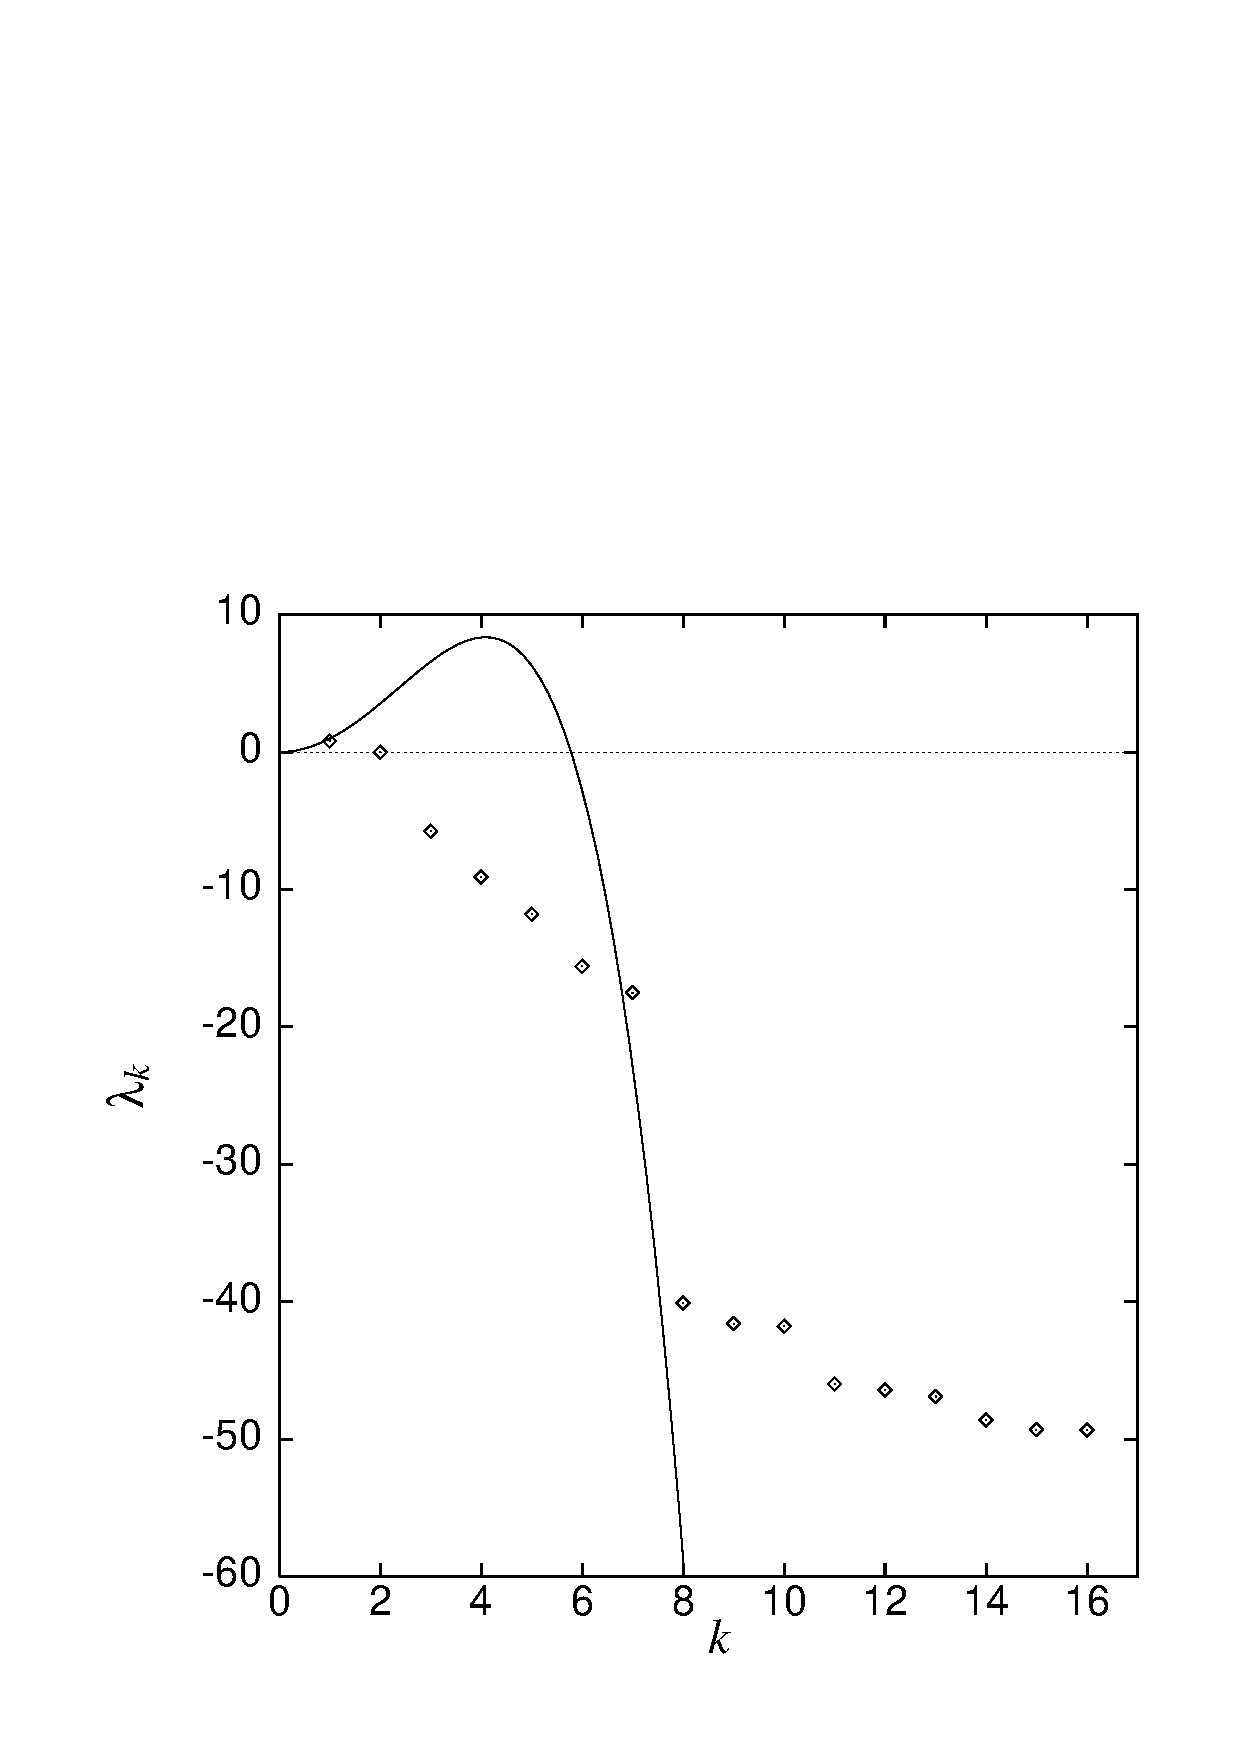
\includegraphics[width=0.40\textwidth]{eigenvalues}
  (b)~\includegraphics[width=0.50\textwidth]{kaz2-PhysModes-b}
  \caption{
    (a)
    Lyapunov exponents $\lambda_k$ versus $k$ for the periodic
    orbit $\overline{1}$ compared with  the stability eigenvalues
    of the $u(x,t)=0$ stationary solution $k^2- \nu k^4$ (from
    \refref{Christiansen97}). $\lambda_k$ for $k \geq 8$ fall
    below the numerical accuracy of integration and are not
    meaningful. Antisymmetric subspace,
    hence no \SOn{2}\ pairing of eigenvalues, $N=16$ real Fourier
    modes, $L=36.31$. One needs to rescale the time to compare
    this to figure (b); -60 in the Lyapunov scale of figure (a)
    corresponds to approx. -1.8 in \reffig{fig:lyapSpec}\,(a).
    (b)
    First 9 Lyapunov exponents $\lambda_j$ for the full
    \statesp, periodic b.c. KS for $L=22$, from a 124 real Fourier
    modes (blue circles) long-time simulation overlayed on
    the \po\ \PO{10.25} (green squares) [Kazz 2011-02-21].
  }
  \label{fig:lyapSpec1}
\end{figure}

% PC 2009-09-12: (a) generated by siminos/figSrc/gnu/lyapSpec.gnu
% PC 2011-03-02: (b) generated by Kazz kaz2-PhysModes-a.png
\begin{figure}
  (a)~\includegraphics[width=0.48\textwidth]{lyapSpec}
  (b)~\includegraphics[width=0.42\textwidth]{kaz2-PhysModes-a}
  \caption{
    (a)
    First 14 Lyapunov exponents $\lambda_j$ for the full
    \statesp, periodic b.c. KS for $L=22$, from a 62 real Fourier
    modes long-time simulation (from \refref{SCD07}).
    (b)
    First 24 Lyapunov exponents $\lambda_j$ for the full
    \statesp, periodic b.c. KS for $L=22$, from a 124 real Fourier
    modes (blue circles) long-time simulation overlayed on
    the \po\ \PO{10.25} (green squares) [Kazz 2011-02-21].
  }
  \label{fig:lyapSpec}
\end{figure}

\begin{description}
\item[2009-09-13 Predrag]
  Sure looks persuasive, see \reffig{fig:lyapSpec}. I have also
  added stability of a periodic orbit from
  \refref{Christiansen97}, for KS on the periodic b.c.,
  antisymmetric subspace, system size $\tilde{L} = 5.8$ close
  to the onset of chaos, 16 real Fourier modes. As (perhaps?)
  discussed in \refref{lanCvit07}, one has to be careful about
  defining the effective system size $\tilde{L}$ for the
  antisymmetric subspace, so these computations are done on
  $L=36.31$ (or $L = 18.155$ if one considers the fundamental
  $[0,L/2]$ domain only). Going from $(L,\nu) =
  (2\pi,0.029924)$ of \refref{Christiansen97} to $(L,\nu) =
  (L,1)$ convention used here requires that the time be
  rescaled as $t \to \nu t$, and the Lyapunov exponents as
  $\lambda_i \to \lambda_i/ \nu = \lambda_i/ 0.029924 $, so -60
  in the Lyapunov scale of \reffig{fig:lyapSpec}\,(a)
  corresponds to approx. -1.8 on the scale of
  \reffig{fig:lyapSpec}\,(b), which would mean that then we
  computed only the first pair of isolated eigenvalues. The
  reason is that for periodic orbits we are computing {\em
    Floquet multipliers} which underflow numerically very
  quickly, so we cannot compute many {\em Floquet exponents}.
  These {\cLv} methods are apparently
  much smarter.

  In \refref{lanCvit07} computations are done at $L = 38.5$,
  but we listed only 4 eigenvalues per periodic orbit, and
  considering hopeless organizational skills on the Lan astral
  plane, I doubt that the full spectra can be rescued from
  Lan's calculations. And, as explained above, probably we cannot
  compute them for periodic orbits.

\item[2009-09-13 Ruslan]
  Here's the expanded list of Lyapunov exponents for KS with $L = 22$:
  0.048,    0.0,    0.0,   -0.003,   -0.189,   -0.256,   -0.290,   -0.310,
  -1.963,   -1.967,   -5.605,   -5.605,  -11.923,  -11.923...
  So, there appears to be 8 `physically relevant' exponents and
  the rest are pairs of hyperbolically separated ones.

  I read
  the papers about these {\cLvs} and I'm not
  sure I understand how they are related to eigenvectors at
  periodic orbits: are they aligned?  I suspect that not quite,
  apart from the most expanding and the most contracting
  direction, the rest are sitting somewhere within the
  subspaces spanned by the $k$ most expanding, or $m$ most
  contracting eigendirections, but not quite aligned with the
  eigendirections themselves.  That's probably why they are
  more appropriately called `Lyapunov vectors'.

\item[2009-09-14 Predrag]
  The `{\cLvs}' are indeed the (right,
  non-orthogonal) eigenvectors of the \jacobianM\ \jMps, as
  defined in ChaosBook, and coincide with Floquet eigenvectors
  for a periodic orbit.

\item[Ruslan] I use 32 complex Fourier modes, so the
  truncated system has 62 degrees of freedom.  The Lyapunov
  exponent calculation is standard (using Gram-Schmidt).  The
  exponents are the same, independent of the method of
  calculation.  I have not attempted to calculate the {\cLvs}. I'm pretty sure that
  orthogonality between {\entangled} and isolated eigenvectors
  applies, but have not checked.

\item[Ruslan]
  It's OK to I email Hong-liu Yang\rf{YaTaGiChRa08}, ask him to rerun his
  {\cLv} spectrum for $L=22$, to see whether he agrees with us.

\item[2009-09-12 Ruslan]
  I have the 62 eigenvalues/eigenvectors for all the RPO/PPO
  I've detected, but for the highly contracting eigenvalues
  the straightforward calculation
  suffers from the numerical noise. We need a
  better method to compute Floquet multipliers. I have now
  checked:   Looks like {Kurt Lust} has proposed one, but I
  cannot get his paper on ``Improved Numerical Floquet
  Multipliers''\rf{Lust01}. If you could
  get it for me, it would be great.
  \phantomsection\label{2013-11-18XD}

\item[2009-09-13 Ruslan]
  ``Structure of characteristic Lyapunov
  vectors in spatiotemporal chaos''\rf{PaSzLoRo09} states
  that characteristic Lyapunov vectors ``reduce to the Floquet
  eigenvectors for a periodic orbit'' and references Trevisan
  and Pancotti\rf{TrePan98}, which I cannot get electronically.

\item[2009-09-14 Predrag]
  I added abstracts of these papers to the reading list above.
  The `{\cLvs}' are indeed the (right,
  non-orthogonal) eigenvectors of the \jacobianM\ \jMps, as
  defined in ChaosBook, and coincide with Floquet eigenvectors
  for a periodic orbit. For a flow they are defined at a given
  \statesp\ point by going back and forward a finite, but
  `sufficiently long' time $t$, and coincide with the Floquet
  eigenvectors if the point is (relative) periodic. I believed
  that for a PDE we cannot go backward, but was wrong; the do
  it by using the segment of forward trajectory stored in
  memory. The reason why one can get the Floquet {\em exponent}
  for arbitrarily long orbit is that the multiplier for eigenvector
  evolved in time is just a number, so taking its logarithm over
  short time segments and
  storing it is trivial, no underflow problems one would get if
  one worked with the Floquet {\em multiplier}. So we should be able
  to keep track of all 62 eigenvectors, redo it for 126 eigenvectors,
  and compare with plots in \refref{YaTaGiChRa08}.
  Ginelli \etal\rf{ginelli-2007-99} are the main
  reference on the `{\cLvs}.' They describe
  the QR algorithm for computing Gram-Schmidt vectors (GSV) and
  recovering the {\cLvs} (CLV) from them.
  What confuses me is that so far all papers refer to $\Lyap_j
  = \eigRe_j + i \, \eigIm_j$ as purely real, and list only
  $\eigRe_j$, but I guess that will be explained somewhere.

\item[2009-09-14 Predrag]
  My initial \reffig{fig:lyapSpec} was not optimal; I have now
  replotted it as in Fig.~4 of
  Yang \etal\rf{YaTaGiChRa08},
  agrees with their 'extensivity' plot for $L=96$ and $192$.

  I prefer $x$-axis to be $j/\tildeL = 2 \pi j/L$, as in
  \reffig{fig:lyapSpecRscld}.

  I do not like the way they count eigenvalues:  due to the $\On{2}$
  2-dimensional irreducible representations
  one should group their $j,j+1$ pairs,
  plot them as a single, two-valued $j$, as in
  \reffig{fig:lyapSpecRscld}. What one chooses to pair for low
  $j$ might be ambiguous, as the nonlinear interactions mix up
  the $\On{2}$ 2-dimensional linearly irreducible representations.
  Reploted as in our much ignored 1997 paper\rf{Christiansen97},
  eigenvalues fall onto $ (2 \pi j/L)^2 - (2 \pi j/L)^4 $
  \eqv\ $\EQV{0}$  stability curve.
  The isolated `{\cLvs}'
  are damped by $-(2 \pi j/L)^4$. I worry that we will not have such
  amicable divorce for plane Couette and pipe flows...

  % PC 2009-09-14: (b) generated by siminos/figSrc/gnu/lyapSpec.gnu
  \begin{figure}
    (a)~\includegraphics[width=0.50\textwidth]{YaTaGiChRa08fig4}
    (b)~\includegraphics[width=0.40\textwidth]{lyapSpecRscld}
    \caption{
      (a)
      Fig.~4 of
      Yang \etal\rf{YaTaGiChRa08}:
      Extensivity of the Lyapunov spectrum for the KS equation with
      periodic b.c.. Inset: number of non-negative exponents (circles),
      Kaplan-Yorke dimension (squares), metric entropy (diamonds,
      multiplied by $50$), and number of {\entangled} Lyapunov vectors (triangles).
      In perfect agreement with
      \reffig{fig:lyapSpec}\,(b) here, plotted the same
      (incorrect) way.
      (b)
      First 14 Lyapunov exponents $\lambda_j$ for the full
      \statesp, periodic b.c. KS for $L=22$, from a 62 real Fourier
      modes long-time simulation (from \refref{SCD07}).
      The same as in part (a) and in \reffig{fig:lyapSpec}\,(b), but
      abscissa is $j/\tildeL = 2 \pi j/L$, and each $j$ labels
      the $\On{2}$ 2-dimensional irreducible representation
      Lyapunov exponents pair.  Full line corresponds to
      the stability eigenvalues
      of the $u(x,t)=0$ stationary solution
      $(j/\tildeL)^2- (j/\tildeL)^4$, for arbitrary system size $L$.
    }
    \label{fig:lyapSpecRscld}
  \end{figure}


  We also see
  that the `{\entangled}' Lyapunov vectors are split into a less contracting 1/2
  and more contracting 1/2 (different slopes in the
  \reffig{fig:lyapSpecRscld}\,(a)). We
  used to think the first 1/2 is the physically important one,
  and say so in the arXiv version 2 of the article.
  We stand corrected.

  The Floquet eigenvectors of our (relative) periodic orbits are
  what they call 'covariant,' so they should fit into their finite back/forth
  time vectors like into a glove, whenever the respective state space
  points are sufficiently close.

  The main point of exploring the ergodic states space hierarchically
  by periodic orbits is to tessellate it systematically, in the most
  uniform way, by neighborhoods (linearized stable/unstable manifolds)
  of periodic points. A periodic solution computed on a small system
  size $L$, periodic b.c. is a solution on any multiple of $L$, and it comes
  together with a smooth family of corresponding solutions for nearby
  $L$'s.

  I see prospects of a long and happy marriage here.

\item[2011-02-04 ES] Talked to Hugues Chat\'{e} and Kazumasa Takeuchi.
  I was at CEA/Saclay for a thesis presentation today, bumped into Chat\'{e}
  and
  \HREF{http://daisy.phys.s.u-tokyo.ac.jp/student/kazumasa/}{Kazz}
  (actually, it was more like invading their offices). Kazz updated me on
  their latest work on Lyapunov vectors. We finally all agreed that we would give
  the periodic orbit - Lyapunov vectors project a second try and arrange to meet
  in Paris. I'll keep you posted.


\item[2011-02-07 ES] Sent Kazz an initial condition for a KS, $L=22$ \po\
  \PO{10.25}.


\item[2011-02-09 Kazz] I tried your initial condition and it works perfectly!
  I also tried to calculate the Lyapunov exponents associated to this {\po}.
  The largest is about 0.03328, right? I'm not yet really sure about this value,
  so it would be nice if you let me know the Lyapunov exponents you know for this {\po}.

\item[2011-02-11 ES] The Lyapunov exponent I have is 0.033163, so you
  are pretty close. In fact this exponent has multiplicity two, and
  there is no other positive exponent for this orbit.

\item[2011-02-11 Kazz] Great! All you are saying (multiplicity, only two positive
  exponents) are exactly what I confirmed with that {\po}. I will soon have all
  the necessary information regarding the {\entangled}/{\transient} Lyapunov vectors for that {\po}.

\item[2011-02-11 Kazz] Which quantities / properties do you have
  analytically / numerically for these \po s in your methods? For instance,
  if we know the time evolution  for a {\po}, we can compute both
  Lyapunov exponents and {\cLvs} as eigenvalues and
  eigenvectors of that operator. Do you have them? Or, the exponent values
  you have are just computed by Bennetin's standard algorithm?

  \renewcommand{\ssp}{x}

\item[2011-02-11 ES] We do not use Bennetin's method, but rather
  something similar to what you just described. However, I am not sure how
  you exactly define the time evolution, so I will describe with
  details what we do (see \refrem{rem:Lyapunov} on \refpage{rem:Lyapunov} above).

  Given an initial condition $\xInit$ and period $\period{p}$ of the prime
  \po\ $p$, we integrate
  the differential equations for the nonlinear flow
  $d\ssp/dt=v(\ssp)$, and a differential equation for the \jacobianM\
  from $t=0$ to $\period{p}$,:
  \beq
  \deltaX(t) = \jMps^t(\xInit) \deltaX_0
  \,, \qquad
  \jMps^t_{ij}(\xInit)
  =  \left. {\pde \ssp_i(t) \over \pde \ssp_j} \right|_{\ssp=\xInit}
  \, .
  \label{hOdes1}
  \eeq
  \beq
  {d\over dt}\jMps^t(\xInit)
  = {\Mvar}(\ssp) \, \jMps^t(\xInit)
  \,, \quad
  \mbox{initial condition~~} \jMps^0(\xInit) = \matId
  \,.
  \ee{Bew_Miaw}
  The {\stabmat} (\velgradmat)
  \beq
  {\Mvar}_{ij}(\ssp) ={\pde \vel_i(\ssp)\over \pde \ssp_j  }
  \ee{DerMatrix1}
  describes the instantaneous rate of shearing of the infinitesimal
  neighborhood of $\ssp=\ssp(t)$
  by the flow.
  We write for its
  eigen\-vectors $\jEigvec[j]$
  (sometimes referred to as `{\cLvs},'
  or, for \po s, as `Floquet vectors')
  \beq
  \jMps_{p}(\ssp)\, \jEigvec[j](\ssp)
  = \ExpaEig_{p,j} \,\jEigvec[j] (\ssp)
  \,,\qquad
  \ExpaEig_{p,j}
  = \sign{p}^{(j)} e^{\eigExp[j]_p \period{p} }
  \,.
  \ee{cplxExpaEig2}
  where $\eigExp[j]_p = \eigRe[j]_p \pm i\eigIm[j]_p$
  and $\sign{p}^{(j)}$ are independent of
  $\ssp$.
  The time-dependent
  $\period{}$-periodic vector fields, such
  as the flow linearized around a \po, are
  described by Floquet theory. Hence
  we refer to a \jacobianM\
  evaluated on a periodic orbit either as
  a {\em \FloquetM} or a {\em monodromy matrix}, to its
  eigenvalues
  $\ExpaEig_{p,j}$ as Floquet multipliers,
  % \refeq{cplxExpaEig2},
  and to $\eigExp[j]_p = \eigRe[j]_p+i\eigIm[j]_p$ as Floquet or
  characteristic exponents.



  The eigenvalues $\ExpaEig_i$ of $\jMps^t(\xInit)$ are
  the Floquet multipliers and its eigenvectors the Floquet eigenvectors
  (the {\cLvs} for \po s).

  Then the $i$th `Lyapunov' exponent is the real part
  $\eigRe[i] = \ln(|\ExpaEig_i|)/ T$ of the Floquet exponent..
  Although we only have the eigenvalues in file, I could easily compute
  the eigenvectors for comparison.

  The problem with this approach is that, while we believe the leading
  eigenvalues to be accurate, the highly contracting ones suffer from
  numerical noise. So it would be hard for us to separate {\entangled} from
  isolated eigenvectors based on this computation alone.


\item[2011-02-11 Kazz] Thank you for the explanation. That is exactly what
  I meant by eigenvalues of the time evolution operator.

  I compute the Lyapunov exponents (and the {\cLvs})
  by Benettin's method (and by Ginelli's one). The only trick is that, each time
  the trajectory $\ssp(t)$ returns to its original position $\ssp(0)$, \ie, at every cycle
  of the orbit, I replace $\ssp(t)$ by its initial value $\ssp(0)$. This is to kill
  numerical noise that would grow and eventually kick the trajectory
  out of the periodic orbit. This method is accurate even for very small
  exponent values.

  \renewcommand{\ssp}{a}

\item[2011-03-10 Predrag] That's OK for the shortest orbits, but
  for longer orbits it will have to be replaced by either section $\to$
  section traversals (see multi-shooting in
  \HREF{http://chaosbook.org/paper.shtml\#cycles}{ChaosBook.org}) or variational methods (see
  \refref{CvitLanCrete02} and
  \HREF{http://chaosbook.org/paper.shtml\#relax}{ChaosBook.org}).

\item[2011-02-18 Kazz]

  \BFIG{1.0}   % width=#1\textwidth
  {kaz-evolution}   % f_name.pdf
  {}   % short caption text
  {    % full caption text
    (a) The \po\ \PO{10.25} [kaz-evolution]
    persists when integrated over 10 prime periods (label $\lambda$
    indicates the leading Floquet exponent). (b) A more unstable
    \po\ is lost after 2 prime periods. (c) A longer
    period \po\ is also lost after a few prime periods.
  }
  {kaz-evolution}   % f-figure-label


  Meantime I show you how my code integrates your {\po}
  (the first three in your
  list), \reffig{kaz-evolution}. Indeed, I cannot integrate
  it even during one period for the second one, which has a large
  Floquet multiplier.

  By the way, the prime period indicated in the file is half the
  full \statesp\ period?
  The space-time plot indicates that...

\item[2011-02-18 ES]
  Yes, this is the convention we follow in our paper\rf{SCD07}, sorry for not
  bringing this to your attention. We define the period $T_p$ to be the
  smallest time such that $u(x+T_p)=\gamma u(x,0)$, where $\gamma$ a
  discrete symmetry transformation (here reflection $R$), see eq. (2.22) in
  our paper and the discussion that follows it. All periodic orbits we
  have found are thus pre-periodic, or \rpo s.
  \PC{really all are \rpo s? I thought about 1/2 of this 40,000 -
    60,000 were not?}
  The evolution
  $T_p$ to $2T_p$ is a repeat of the pre-periodic orbit which
  is periodic in this case, as $R^2=1$ (and thus we can take the period to be $T_p$
  rather than $2T_p$). You should take advantage of this
  when computing Lyapunov exponents, integrating only from $0$ to $T_p$ and
  then applying $R$ to $u(x,0)$ to get a new initial condition, before
  integrating from $T_p$ to $2T_p$ and so on. I should have mentioned this
  convention, but it is by now second nature to me.

  By the way, what method do you use for integration? For the third
  orbit, could you please compute $||u(x,2T_p)-u(x,0)||$ (or
  $||u(x,T_p)-Ru(x,0)||$ where $R$ is reflection)? The choice of norm should
  not be crucial. I ask because I think this is the best indicator of
  reproducibility of the periodic orbits. For the second orbit, if you
  could compute $||u(x,T_p)-Ru(x,0)||$, it might tell us that the
  difference is not as large as the figure suggests.

\item[2011-02-21 Kazz]

  \BFIG{1.0}   % width=#1\textwidth
  {kaz-evolution2}   % f_name.pdf
  {}   % short caption text
  {    % full caption text
    {\po} \PO{10.25} [kaz-evolution2]
  }
  {kaz-evolution2}   % f-figure-label


  Thanks for the kind explanation. I should have read your
  paper more carefully... I shall do this very soon.

  Here I attach a figure, \reffig{kaz-evolution2}, showing
  how a measure of the distance between a
  trajectory and an orbit grows in time. The same trajectories and the orbits
  as in the figure I send you last Friday are used. The dashed lines are the
  growth rate expected from their Floquet multipliers and agree well with the
  actual growth of the distance. Indeed, even for the second orbit the trajectory
  stays close to it up to time $~2T_p$.

\item[2011-02-22 ES] In the last set of figures (evolution2.pdf), is $u(x,t)$
  an orbit resulting from perturbing the initial condition of the periodic orbit?

\item[2011-02-23 Kazz] Concerning your question, the initial condition for u(x,t)
  is exactly the one you sent to us. Just I integrated it and measured how
  it deviates from the orbit because of the numerical noise.


\item[2011-02-20 Predrag] to Kazz:
  I'm very glad that you and Evangelos are looking at the KS periodic solutions.
  Attached is \refsect{sect:LyapKS} from out blog
  (you probably have this already, but
  I am not quite sure) - if you plot all cycle Floquet multipliers, can you try to
  also plot them in the way suggested in my notes (it differs a bit from how you
  had plotted them in Yang \etal\ paper\rf{YaTaGiChRa08})?
  I was pleasantly surprised how well one
  could see the {\entangled}/isolated boundary already for $L=22$.


  \BFIG{1.0}   % width=#1\textwidth
  {kaz2-PhysModes-cd}   % f_name.pdf
  {}   % short caption text
  {    % full caption text
    Compare with frames (d) and (e) in \reffig{fig:lyapSpecCLG}.
    {\po} \PO{10.25} [kaz2-PhysModes-cd]
  }
  {kaz2-PhysModes-cd}   % f-figure-label

  \BFIG{1.0}   % width=#1\textwidth
  {kaz4-VectCompar}   % f_name.pdf
  {}   % short caption text
  {    % full caption text
    {\po} \PO{10.25} [kaz4-VectCompar]
  }
  {kaz4-VectCompar}   % f-figure-label

  \BFIG{1.0}   % width=#1\textwidth
  {kaz5-AngleTimeSeries}   % f_name.pdf
  {}   % short caption text
  {    % full caption text
    {\po} \PO{10.25} [kaz5-AngleTimeSeries]
  }
  {kaz5-AngleTimeSeries}   % f-figure-label

  \SFIG{kazUPOa}   % width=#1\textwidth
  {}   % short caption text
  {    % full caption text
    {\po} \PO{10.25} [kazUPOa]
  }
  {kazUPOa}   % f-figure-label

\item[2011-02-21 Kazz]
  I (with spirits of Hugues Chat\'e and Francesco Ginelli hovering above me)
  have integrated some of
  them and computed a number of quantities to elucidate the
  {\entangled}/isolated separation of Lyapunov vectors. Here I show a
  summary of preliminary results. I also have some questions to ask you
  (see the end of the mail for them).


  \textbf{Results}

  Here we concentrate on (1) a chaotic trajectory generated from a random
  initial condition, and (2) the first periodic orbit \PO{10.25},
  $\period{p}=10.25336729174627$ in the list
  Evangelos sent to me (called "{\po}a" in the attached
  figures). The numerical integration of the {unstable \po} is done by replacing the
  trajectory on each period by the initial condition of the {unstable \po}.
  \PC{to Evangelos - do we have a naming convention in \refref{SCD09b}
    and/or \refref{SiminosThesis} that we could follow here,
    instead of renaming every \po? {\bf ES:} No. We use
    $(T_p,\ell_p)=(.,.)$ to refer to a \rpo.}

  % PC 2011-03-02: (b) generated by Kazz kaz2-PhysModes-b.png
  \refFig{fig:lyapSpec1}\,(b)
  and
  % PC 2011-03-02: (b) generated by Kazz kaz2-PhysModes-a.png
  \reffig{fig:lyapSpec}\,(b)
  show the Lyapunov spectrum for
  the trajectory and the {unstable \po}.

  For the {unstable \po} the exponents are
  given by the Floquet multipliers, as indeed confirmed quantitatively,
  while for the chaotic trajectory they are different from but close to
  those of the {unstable \po}, \refFig{fig:lyapSpec1}\,(b).
  % (top right figure).
  Increasing the index, we
  see the appearance of the step-wise structure (top left figure) like in
  our Yang \etal\rf{YaTaGiChRa08} PRL.

  \refFig{kaz2-PhysModes-cd} shows the hyperbolic isolation of the {\entangled} and
  isolated Lyapunov vectors (similar to frames (d) and (e) in \reffig{fig:lyapSpecCLG}
  from our PRL); they
  CANNOT be defined solely from the Lyapunov exponents.). The quality of
  the data is not satisfactory because of the present length of the
  simulation, but we can see that there are at most 11 {\entangled} Lyapunov vectors.


  \refFig{kaz4-VectCompar} compares the {\cLvs} on the
  chaotic trajectory with the Floquet vectors of the {unstable \po}. I monitored the
  chaotic trajectory and used the instant when it gets closest to the {unstable \po}
  during the simulation. The inset of the top left figure shows the
  snapshot of the trajectory (blue) and the {unstable \po} (red) at that instant.

  The other three subpanels compare the vector structure at the same
  instant. Here the spatial shift between blue and red is already taken
  into account, so that you can directly compare the two profiles. The
  bottom two figures show the 6th and 9th Lyapunov vectors, which correspond to
  real-valued Floquet multipliers of the {unstable \po} (thus Oseledec subspace is
  not degenerated). We can see that the vectors of the chaotic trajectory
  become quite close to the {unstable \po} counterparts (but not exactly; some are
  better, others are not as good). For the Lyapunov vectors that correspond
  to complex conjugate pairs of the Floquet multipliers, e.g. 1st and 2nd
  ones, we have to compare a vector of the trajectory with arbitrary
  linear combinations of the 1st and 2nd {unstable \po} vectors. Indeed, we can find
  a combination that gives a structure similar to the vector of the
  trajectory.

  In short, as a chaotic trajectory wanders among {unstable \po}s, the vectors of the
  trajectory change their shape incessantly to follow the vectors of the
  closest {unstable \po} at each instant.


  Now, the question is whether we can unambiguously define the {\entangled}
  and isolated Lyapunov vectors for each periodic orbit, or not. We don't know how to
  do this, because the angle between any Lyapunov vectors
  of {unstable \po} varies periodically and thus does not reach 0 or
  $\pi$ forever.

  Moreover, we find that the hyperbolicity properties crucially depend on
  the quality of the periodic orbit. See
  \reffig{kaz5-AngleTimeSeries}, which shows
  time-series of angles between given pairs of the Lyapunov vectors of the
  {unstable \po}. Although the angle between Lyapunov vectors of index $\geq 11$ (correspond
  to isolated Lyapunov vectors for the chaotic trajectory) stays close to $\pi/2$ with a
  seemingly trivial time-evolution, the numerically computed angle is not
  strictly $\pi/2$ and is subject to a very slow convergence (see the middle
  panel). To test, I added a noise to the initial condition of the {unstable \po} and
  computed the same quantities. While the angles for index $\leq 10$ do not
  show significant changes, those for index $\geq 11$ show {\transient}
  oscillations with long periods.

  This is why we think that the quality of the periodic orbit is crucial.
  It could be that, if we had an initial condition with infinite
  precision, the angle for index $\geq 11$ are strictly orthogonal, and thus we
  could define the isolated Lyapunov vectors from this strict orthogonality.


  \textbf{Questions}

  1) We wonder if we may define the {\entangled} and isolated Lyapunov vectors for
  periodic orbits. Do you have any ideas, in particular from the viewpoint
  of the Floquet multipliers and eigenvectors?

  2) As shown above, the quality of the {unstable \po} initial conditions turns out
  to be crucial. Do you have data with better resolutions? Or, is it
  numerically difficult to compute {unstable \po}s with very high resolutions?

  That's all for now. Any comments / questions are of course welcome!


  \textbf{Kazz to Predrag} I made a plot of the Lyapunov spectrum of
  the {unstable \po} (the same one as above) in the same way as you did. See \reffig{kaz{\po}a}
  and {\po}a-lyap.dat (below). I hope this is the one you wanted.

  \begin{table}[h!]
    \caption{The Floquet exponents of periodic orbit \PO{10.25}.
      [computed by Kazz 2011-02-18].
    }\label{tab:ks22po10.25FloqExp}
    \begin{center}
      \begin{tabular}{c}
        3.3274529258200000e-2    \\
        3.3273022876699997e-2    \\
        1.2294744377000001e-5    \\
        -1.3236540275600000e-5    \\
        -7.2634814842399998e-5    \\
        -2.1629227416399999e-1    \\
        -2.6517234146000002e-1    \\
        -2.6516527982799998e-1    \\
        -3.3072168309500000e-1    \\
        -1.9602739059100001    \\
        -1.9673554279600001    \\
        -5.6025023421000002    \\
        -5.6042396292200003    \\
        -1.1925106699200001e+1    \\
        -1.1925523679299999e+1    \\
        -2.2011597078699999e+1    \\
        -2.2011657848500001e+1    \\
        -3.7116197744200001e+1    \\
        -3.7116202659300001e+1    \\
        -5.8760926784699997e+1    \\
        -5.8760926787599999e+1    \\
        -8.8935807811399997e+1    \\
        -8.8935807884699997e+1    \\
      \end{tabular}
    \end{center}
  \end{table}


\item[2011-03-05 Predrag to Kazz] I do not understand your \po\ calculations.
  For this short orbit I expect everything - all Floquet multipliers and
  Floquet vectors to be good to a machine precision, or at least to - let's say -
  $10^{-6}$?

\item[2011-03-05 Predrag]
  I find
  \reffig{fig:lyapSpec1}\,(b) amazing. The {\po} \PO{10.25} is
  only exploring the $\infty$-dimensional \statesp\ as the
  shortest 1-dimensional loop, while the chaotic trajectory is
  wondering over the whole 11-dimensional (say Parisians) strange attractor
  (inertial manifold) and still the entangled eigenvalues are so close.

\item[2011-03-07 Hugues]
  That's because the {\po} \PO{10.25} is the least unstable of all
  \po s.

\item[2011-03-07 Predrag] Easy to say, but in \refref{SCD07} we have
  not noticed any concentration of the natural measure in the neighborhood of
  this \po. That is perhaps because we have not quotiented
  $\pS \to \pSRed = \pS/\SOn{2}$, and $\SOn{2}$ drifts can easily
  mask a much simpler strange attractor\rf{SiCvi10,FrCv11}.


\item[2011-03-04 Evangelos]
  I really can't follow this tessellation idea. My motivation to be
  involved with this project at this point developed while reading Roweis
  and Saul\rf{RoSa00}. I believe what we ought to do should be very close
  to their way of thinking: construct linear local charts (bases) and then
  bring them together to construct a global curvilinear embedding. In
  contrast to their pattern recognition, empirical way to construct the
  local charts, we can use information from the {\cLvs}.

\item[2011-03-05 Predrag]
  I agree in principle.
  See also {\bf [2010-12-06 PC]} in \texttt{siminos/blog/atlas.tex}

\item[2011-03-04 Evangelos]
  I would prefer to work with \KS\ in the antisymmetric subspace, so that we do not
  have to worry about the translational symmetry (remember that the periodic
  orbits for $L=22$ are in the full space, rather that in the antisymmetric
  subspace).

\item[2011-03-07 Hugues]
  I agree, shifts are killing us.

\item[2011-03-05 Predrag]
  I agree.
  \PCedit{
    [revised 2011-03-10: I disagree, see comment below]
  }


\item[2011-03-04 Evangelos]
  The local charts can be provided by the {\entangled} {\cLvs} computed on a set of the most important \po s. Then we only need
  to implement the final step in the procedure of Roweis and
  Saul\rf{RoSa00}, which involves solving a minimization problem for the
  global coordinates and should be computationally tractable if a truly
  low-dimensional embedding exists.

\item[2011-03-05 Predrag]
  We cannot tessellate with \po s; we can only work with \emph{periodic
    points}, hence we need to understand what Floquet vectors (AKA `covariant
  Lyapunov' vectors evaluated on \po s) tell us about the `physical
  dimension' of the local {\PoincSec}.

\item[2011-03-04 Evangelos]
  How could a trajectory be confined to a {\PoincSec}? You seem
  to talk about local charts in \refsect{sec:chart}, rather than {\PoincSec s}.

\item[2011-03-05 Predrag]
  Ant is not following a \emph{trajectory}, ant is moving \emph{transversely}
  to the time flow, for example: if the continuous time trajectory has one
  unstable eigen-direction, it sweeps out a 2-dimensional unstable manifold,
  whose {\PoincSec} is 1-dimensional curve that the ant could follow.

\item[2011-03-04 Evangelos]
  If we manage to use local {\PoincSec s} to reduce the flow to a
  discrete map (or maps) before applying this procedure, we would then only
  need one (or a few) representative point(s) per periodic orbit for our
  local charts, rather than points along the full orbit. However, we know
  this is tricky to do in a high-dimensional space, before an embedding is
  available.

\item[2011-03-05 Predrag]
  \HREF{http://en.wikipedia.org/wiki/String_Quartet_No._16_(Beethoven)}
  {Es muss sein!} No sense can be made out of a collection of \po s unless
  they and their Floquet vectors are reduced onto  {\PoincSec s}.

\item[2011-03-04 Evangelos]
  In any case, while I can see many local {\PoincSec s} working
  together, either before or after the global coordinates are found, I
  cannot see how a tessellation as you describe it here would work.
  {\PoincSec s} are designed to pierce the flow (so the ant we follow
  would leave the section immediately) and good sections should be
  transverse, not tangent to the attractor.

\item[2011-03-05 Predrag] Grave misunderstanding. The continuous group
  that is being reduced by {\PoincSec s} is the evolution in time.
  After the reduction of continuous time to discrete time, what remains are
  the affine hyperplanes (local {\PoincSec s}) which are
  \emph{tangent} to the strange attractor; the ant is not crawling in the
  time direction, she is crawling (for example) along the unstable manifold
  heteroclinic section as it is seen within the {\PoincSec s}, not the
  time trajectory traced out in the full \statesp.

\item[2011-03-02 Evangelos] First meeting's wisdom:
  \begin{itemize}
  \item[2011-03-02 Parisians] We
    \HREF{http://en.wikisource.org/wiki/Gargantua/Chapter_XVI}{Parisians}
    all agree that it's best to work on antisymmetric subspace KS.

  \item[2011-03-10 Predrag]
    \PCedit{
      I'm very worried about this development. We have settled in
      \refref{lanCvit07} on $L=22$ as the smallest system size for which the
      translationally invariant KS is empirically `shmurbulent.' We cannot work
      with \KS\ in the antisymmetric subspace at $L=22$, because there is no
      chaos there - that's why Lan and I worked\rf{lanCvit07} at  $L = 38.5$.
      We cannot work with \KS\ with the fixed $u(0)=u(L)=0$ boundary conditions
      at $L=22$, because there will be no shmurbulence there either - when the
      ends are pinned down, one needs a larger cell to approach the onset of
      shmurbulence, that's why the antisymmetric subspace required going up to
      $L = 38.5$. Besides, for small $L$ the boundary effects will dominate the
      dynamics, the \statesp\ geometry will be very different, and what we
      learn there will not scale to larger $L$. What was so elegant about
      analysis\rf{SCD07} of  $L=22$ system is that the geometry of the
      \statesp\ was so much more beautiful than what it is for the $L = 38.5$
      antisymmetric subspace. Since then we have lost fear of continuous
      symmetries\rf{SiCvi10,FrCv11}. And continuous symmetries are the
      physically interesting case. In summary, going to fixed b.c. is ugly,
      unphysical, and to add insult to injury, it would necessitate a whole new
      fishing expedition, abandoning all the wisdom we already have in the
      $L=22$ case.
    } %end \PCedit{


  \end{itemize}



\item[2011-03-02 Evangelos] First meeting's numerics:
  \begin{itemize}
  \item Evangelos will do the shooting for periodic orbits
    (we need to decide on system size). He hopes he will find the time \ldots
  \item Kazz uses an implicit second order Adams(-Moulton) method (see post of
    2011-03-09), with pseudospectral space discretization.
    He uses some prescription for anti-aliasing, in order to keep the large wavenumbers
    and corresponding isolated Lyapunov vectors uncontaminated. Uses numerical
    recipes for FFT. (ES suggests switching to FFTW as numerical recipes FFT is
    known to be unreliable in double precision.)
  \item Evangelos uses explicit fourth order Runge-Kutta with exponential
    time differencing (see \refref{ks05com}) and pseudospectral space
    discretization. He uses brute force anti-aliasing (increases resolution
    to the point that only Lyapunov vectors already at round-off are affected by
    aliasing). He uses FFTW.
    \PC{can you identify this pesky reference 'ks05com'?}
  \item We agreed that a good strategy would be that Kazz implements a simple
    Newton routine, so that he can refine the orbits I give him. I've
    pointed him to Chaosbook chapters, my own first year report on Newton's
    method for periodic orbits and my thesis.
  \item I've also agreed to give Kazz the backbone of my integrator routines
    (and also pointed him to \refref{ks05com}). Kazz is suspicious towards
    Trefethen's algorithm, he thinks that the integrating factor trick might
    lead to under-resolved large wavenumbers and problematic isolated
    Lyapunov vectors (and that the implicit method performs better in this
    respect). I can't argue in favor of one or the other integrator.
  \item I am also thinking to try to implement anti-aliasing and see
    if agreement improves.
  \end{itemize}

\item[2011-03-09 Kazz] to Evangelos:
  Before your mail I made a code to improve the quality of the periodic orbits
  and it works very well. Now, with my integrator, the norm of distance
  (with square root) after one cycle is on the order of $10^{-13}$ for the orbit
  I focus on, and the trajectory stays nearby over $40$ periods, to be compared
  with $10$ for the original orbit data. I restarted all the calculations
  with this improved orbit.

  To answer your question, my code uses the splitting method with the
  2nd-order implicit method
  \HREF{http://en.wikipedia.org/wiki/Linear_multistep_method}{(Adams-Moulton)}
  for the linear terms and the 2nd-order Runge-Kutta
  \HREF{http://en.wikipedia.org/wiki/Heun\%27s_method}{(Heun method)}
  for the nonlinear term.

  For the aliasing, I use at least $(3N+1)$ spatial points when computing
  the nonlinear term, where $N$ is the wavenumber cutoff of the Fourier modes.
  Under this condition the pseudospectral method is exact
  (equivalent with the spectral method apart from the computational cost).

  \BFIG{1.0}   % width=#1\textwidth
  {kaz-fig-temp}   % f_name.pdf
  {}   % short caption text
  {    % full caption text
    {\po} \PO{10.25} [kaz-fig-temp]
  }
  {kaz-fig-temp}   % f-figure-label

\item[2011-03-10 Kazz] To refine the orbits I use Newton's method,
  but I adapted it to apply to half a period, playing with the reflection
  symmetry. That is to say, instead of considering
  \[
    (I-J(u))(u'-u) - vt = -(u-f(u))\,
  \]
  I use
  \beq
  (R-J(u))(u'-u) - vt = -(Ru-f(u))\,
  \ee{eq:preper-newt} where $R$ is the operator
  for the reflection, i.e., $Ru(x) = -u(-x)$.
  It is better, not only because the integration time is half, but also because
  the reference coordinate $x_0$ for the reflection $u(x,t)=-u(x_0-x,t+T_p)$
  is automatically set to be 0.

  That said, I looked at the results from the refined orbit, and found
  that the results do not change. The angle between {\transient} Lyapunov vectors oscillates
  always with a finite amplitude.

\item[2011-03-10 ES] My bad here, I forgot to mention to Kazz that we
  use \refeq{eq:preper-newt} for pre-periodic orbits \ldots

\item[2011-03-10 Ruslan] {\em Comment on the numerical approximation of the KS flow}\\
  I would suggest not to worry too much about the accuracy of the numerical
  approximation of the KS flow.  Instead, it is better, in my opinion, to
  adopt the viewpoint that one investigates the properties not of the KS
  flow, but of the map defined by the numerical integrator of the \KSe,
  which approximates the solutions of the \KSe.  As long as the orbits of
  the map resemble the solutions of the flow (think of it in terms of
  shadowing), the results of our investigation of the map will faithfully
  represent those for the KS flow.  So, it doesn't matter whether one
  investigates the Kassam-Trefethen map or the Adam-Moulton-RK map: the
  qualitative picture will be the same.

  The neat thing about Kassam-Trefethen map is that it solves the linear
  part of the KS flow exactly, thus eliminating the problem of the
  stiffness of the linear part, and thus allowing to use a much larger time
  step.  Implicit Adams-Moulton also deals with the stiffness, but it
  solves the linear part only approximately, so it is likely to be less
  accurate if used with the same time step.

  From the same viewpoint, there is also no need, in my opinion, to use
  anti-aliasing.  If a better approximation of the KS flow is needed, just
  include more modes into the map and decrease the time step.  Of course,
  if Kazz already implemented anti-aliasing, then there is no harm in using
  it, provided it doesn't increase the flops count too much.

\item[2011-02-21 Kazz]
  If the isolated Lyapunov vectors of
  {unstable \po}s are strictly orthogonal, it means that the \jacobianM\ for a
  cycle can be decomposed to two parts, one of which would be an
  orthogonal submatrix. Does that seem likely to you?

\item[2011-03-10 Ruslan]
  I don't see why we should expect higher Lyapunov vectors to be {\em
    exactly} orthogonal.  Since all Lyapunov vectors in the \KSe\ are coupled
  though the nonlinear term, the deviation from orthogonality should be
  proportional to the strength of this coupling.  Of course this coupling
  is very weak for higher Lyapunov vectors and decreases exponentially with
  increasing mode number.  But if we measure with sufficient resolution,
  which is what Kazz does, we'll observe the deviation from orthogonality
  for any higher mode, whether anti-aliased or not.  Or am I wrong?

\item[2011-03-10 Predrag] My belief too. There is no reason to require
  \transient\ Floquet vectors to be pure, orthogonal Fourier modes: all we
  need is that perturbations along these directions are pushed back into
  the attractor without being entangled along it...

\item[2011-03-11 Ruslan] It seems to me that the behavior of the isolated
  Lyapunov vectors in the \KSe\ is rather easy to understand.  Since they
  are essentially generated by the linear part of the \KSe, they will be
  nothing else but the Fourier modes living in mutually orthogonal planes.
  That is, they are the eigenvectors of the \jacobianM\ of the trivial
  equilibrium $u = 0$, just slightly perturbed by the nonlinear coupling.
  But since, as I already said, this perturbation decays exponentially with
  the mode number, it is negligible for high enough modes.  So, to answer
  Kazz's question, the strongly contracting eigenvectors of the \jacobianM\
  of a cycle should be essentially orthogonal to one another as well as to
  the subspace spanned by the expanding and weakly contracting eigenvectors
  (i.e. the subspace where the {\entangled} Lyapunov vectors live).

\item[2011-06-28 Evangelos]
  Met with Kazz at \HREF{http://cct11.cpt.univ-mrs.fr/}{CCT11 conference}
  at Marseilles and discussed about their progress with Lyapunov vectors
  for periodic orbits. To my understanding, the main points are: Kazz
  \etal, identify generic orbits that come close to a periodic orbit. They
  use the vector defined by the points of minimal distance along these two
  trajectories as a local approximation to the ``inertial manifold.''
  However, some of the Lyapunov vectors computed along the periodic orbit
  and the generic trajectory are not identical or even similar (at the
  points of minimal distance). Kazz argues that it is not possible to
  define {\entangled} and isolated modes for periodic orbits (in his numerics
  the number of physical dimensions inferred from a periodic orbit would
  be, in general, different from the number of physical dimensions inferred
  from a generic orbit).

\item[2011-06-28 Predrag] I will deal with this in bits:
  First, not being in frequent contact is not working for me - I
  do not know what is being computed or why. Are we in the \KS\
  antisymmetric subspace at\rf{lanCvit07} $L = 38.5$, or the
  full space at $L=22$? As I wrote above in the {\bf 2011-03-10}
  entry, I believe we cannot work in the \KS\ antisymmetric
  subspace at $L=22$, as there is no shmurbulence there. If Kazz
  is integrating trajectories in the full space at $L=22$, he
  \emph{must} quotient the translational $\SOn{2}$, otherwise
  there is no way to define the (locally minimal) Euclidean
  distance(s) between a \po\ and a generic long-time trajectory\rf{FrCv11}.

\item[2011-07-22 Evangelos] Spatial shift in eq. (2) of 2011-07-21 draft seems
  to take care of that, although this approach seems to be somewhat inefficient.
  A question: Is the spatial shift a multiple of the spatial discretization step?
  If yes, then this means that you probably overestimate the distance of minimum
  approach based on eq. (2). You should then refine the comparison by introducing
  a local slice as in \refrefs{SiCvi10,FrCv11}.


\item[2011-06-28 Predrag]
  Using ``the vector defined by the points of minimal distance along these two
  trajectories as a local approximation to the inertial manifold'' makes no sense to me.
  The local approximation to the inertial manifold is spanned by the transverse
  \po\ Floquet eigenvectors at that periodic point (simplest to take a local {\PoincSec}
  normal to $\vel(\ssp)$ at $\ssp$).

\item[2011-06-28 Predrag]
  If the generic trajectory is close the periodic point in a direction
  along its unstable manifold, it is close. If it belongs to a different fold of the
  unstable manifold, than it is far away and can have quite different local
  tangent space.

  If the two points are close, the periodic point tangent space
  eigen-directions should be close to the {\cLvs} at the nearby generic
  point, as they are probing the same stable / unstable manifolds structure in the
  linear neighborhood that includes them both.

\item[2011-07-22 Evangelos]
  I've actually raised the objection about the generic trajectory belonging to a
  different fold of the unstable manifold of the periodic orbit to Kazz in our
  discussion at Marseilles. His
  counter-argument is, I think, based on figure 5(c) of 2011-07-21 draft. His
  claim is that since the angle tends to zero as the generic trajectory approaches
  the periodic orbit the approach has to be along the unstable manifold.
  However, I am not convinced that we can numerically tell the difference
  if the minimum distance along the local unstable
  eigen-direction is much larger than the separation of folds of the unstable
  manifold. Kazz, could you please clarify and give as more insight?

\item[2011-06-26 Kazz] It is not possible to
  define {\entangled} and isolated modes for periodic orbits (in my numerics
  the number of physical dimensions inferred from a periodic orbit would
  be, in general, different from the number of physical dimensions inferred
  from a generic orbit)

\item[2011-06-28 Predrag]
  A short \po\ might be quite hyperbolic, \ie\ never get close to any
  tangencies (small angles between leading Floquet eigenvectors). The longer ones
  should probe heteroclinic tangencies a bit better...

\item[2011-08-09 Predrag] For comments to Takeuchi and Chat\'e\rf{TaCh11}
  \emph{Can the inertial manifold be captured by unstable periodic
    orbits?}, see {\bf [2011-07-21]} entry, \refsect{sec:TaCh11}.

\item[2011-08-17 Evangelos]
  I've just arrived to Dresden and found out that Hugues will
  spend a year in the Institute heading a study group and Kazz will come
  here for a workshop. So I'll get a chance to talk discuss with them.

\item[2011-08-17 Evangelos]
  Kazz works in full space but studies
  periodic orbits. You and me know that relative periodic orbits are the
  relevant objects that are expected to capture the dynamics in presence
  of translational symmetry, so why not try them instead?

\item[2011-08-17 Predrag]
  Here is my proposal to you and Ruslan. You have some 40,000 \rpo s. Why
  not take a point on the Kazz favorite cycle
  \PO{10.25} as the template $\slicep$, and pick from
  the 40,000 \rpo s the set of the closest ones to it in its slice. As they
  are cycles in {\pSRed} you need to also make a local {\PoincSec}
  through template point $\slicep$ (within the slice), normal to the
  velocity vector $\velRed(\slicep)$, to find the closest passage. Some are
  probably as close as the Kazz chaotic trajectory closest passage. For
  each of the close ones you have the 9-12 leading eigenvectors, their
  orientations information on where you are on stable/unstable manifolds,
  and their relative separation vectors. Those Kazz will need to check,
  show they are in the `physical' 9 dimensions.

\item[2011-08-25 Hugues, Predrag]
  Evangelos is here sitting with me, and we tried to figure out what you
  meant exactly. We have a proposal for something (hopefully) close to your
  idea:
  \begin{enumerate}
  \item Take Kazz `favorite orbit' \PO{10.25} (or a few of them). For
    this one, we know the vectors pretty well, all along the cycle.
    {\bf [2011-08-25 Predrag]} Pick a \emph{specific point}
    $\ssp_{\PO{10.25}}$ on the Kazz favorite cycle \PO{10.25} as the
    \template\ $\slicep = \ssp_{\PO{10.25}}$. As you will use $\slicep$
    to fix both the slice and the {\PoincSec}, some choices might
    be better than others: I am not sure how to pick this starting point.
    The local {\PoincSec} through template point $\slicep$ (within
    the slice) is picked normal to the velocity vector
    $\velRed(\slicep)$. The Floquet vectors are computed \emph{within}
    both the slice and the {\PoincSec}; the computation is
    described in the ChaosBook Section 5.3
    \HREF{http://chaosbook.org/chapters/invariants.pdf} {Stability of
      \Poincare map cycles}.


  \item Take the 40000 or so \po s available; for each near one,
    determine the closest point to the \template\ point \PO{10.25} (by
    "slicing" or more pedestrian methods).
    {\bf [2011-08-25 Predrag]} Slicing + Poincar\'e is, \emph{by
      definition}, the closest distance between the \emph{\template\
      point} $\ssp_{\PO{10.25}}$ and the \po\ (or \rpo) $p$. There are
    \emph{no} more pedestrian methods that work. If they exist, please
    enlighten me; what Kazz does is unecessarily laborious and
    inaccurate. Nothing can be said about the topology of inertial
    manifold unless symmetry reduction is implemented first. We have
    implemented slicing on 3D Navier-Stokes full resolution pipe flow
    ($10^5$ dimensions), so what do you fear about slicing $10^2$
    dimensions but the fear itself?


  \item At this closest point $\ssp_p$ on {\po} $p$, we have a minimal
    distance $\|u_p\|$ to the \emph{\template\ point} $\ssp_{\PO{10.25}}$,
    and the corresponding difference vector $u_p$. We can then compute the
    angle between vector $u$ and the subspace spanned by the $n$~first
    Floquet vectors of the \template\ point  \PO{10.25} (at the point of
    closest distance of course).

  \item Plot this angle (or its mean), as a function of $\|u\|$ for the
    nearest 10-100 out of the 40000 (relative) \po s. This could give the
    same result as our Fig.5c: if you take fewer vectors than the
    `physical' number, then the angle is bounded away from zero, but if you
    take the `right' number (or more), then the angle goes linearly to zero
    with $\|u\|$. Throw away `near' \po s which are near in Euclidean
    metric, but are isolated and off the local tangent space to the
    `{\entangled}' manifold.

  \item This set of periodic \emph{points} covers a linearized tile
    around the \template\ point \PO{10.25}. Now take one of them toward the
    edge of the tile as the new \template\ point, and repeat. If that one
    has a small physical dimension for a finite neighborhood, we have a
    chance of tiling the entire inertial manifold as in
    \reffig{fig:Tesselate}.
  \end{enumerate}
  If, indeed, similar behavior is observed from just looking at \po s, then
  the dimension of the ``physical manifold'' has been indeed calculated
  using strictly only \po s.....  ah ah!

\item[2011-08-17 Evangelos]
  By the way, do you understand how Kazz handles spatial shifts? After a
  long exchange of emails it seems that I don't.

\item[2011-08-17 Predrag]
  I believe he does it what was the standard way before the invention of
  slicing. Following ChaosBook:

  {\SOn{2} irreducible representations:}
  Expand a smooth periodic function $u(\gSpace + 2\pi) =
  u(\gSpace)$ as a Fourier series
  \beq
  u(\gSpace) = a_0 + \sum_{m=1}^\infty \left(
    a_m \cos m \gSpace + b_m \sin m \gSpace
  \right)
  \,.
  \ee{FourierExp}
  The matrix representation of the \SOn{2}\ action
  on the $m$th Fourier coefficient pair
  $(a_m,b_m)$ is
  \beq
  \LieEl^{(m)}(\gSpace') \,=\,  \left(\barr{cc}
    ~\cos m \gSpace'  & \sin m \gSpace' \\
    -\sin m \gSpace'  & \cos m \gSpace'
    \earr\right)
  \,,
  \ee{SO2irrepAlg-m}
  For each chaotic trajectory point he runs $\theta$ in some interval and
  finds the minimal distance to the periodic point (their paper says that).
  Though I am not sure that this is what he really does.

  Sorry, getting too late - need to go to bed.

\item[2011-09-12 Evangelos] Talked with Kazz, Hugues and Francesco (2011-09-12).
  The main points are:
  \begin{itemize}
  \item No one wants to discuss slice fixing details, so I did not insist.
  \item I explained [2011-06-28 Predrag] comment on the discrepancy of some of the
    Lyapunov vectors as computed on a chaotic trajectory and a periodic
    orbit in Fig 3 of \rf{TaCh11}. Francesco says a math paper shows
    continuity of Lyapunov vectors but he will check the assumptions
    (and will send me the reference).
  \item We agreed to follow Predrag's suggestion and check the
    role of non-hyper\-bolic periodic orbits. Kazz will try to identify
    regions in state space where hyper\-bolicity seems to
    be violated and will give me some guesses for periodic orbits.
  \end{itemize}

\item[2011-09-12 Predrag] This aversion to slicing is a pain. None of the
  problems with continuous symmetries can be done without it, but so far I
  have only gotten Willis converted\rf{ACHKW11}
  \HREF{http://www.cns.gatech.edu/~predrag/papers/ACHKW11.pdf}
  {(a rough draft is here)}, and that is because in pipes the streamwise
  continuous symmetry is $\SOn{2}$ (no discrete reflections) so
  \emph{nothing} can be done without slicing. Not slicing in KS, CLGe, and
  \pCf\ is simply wrong - one cannot organize the \statesp\ without it. My
  impression from the {\bf [2011-07-27 Kazz 2 Evangelos]} comments in
  \refsect{sec:TaCh11} is that Kazz is confused about what slicing
  is, but believes he understands it. Can you get EVO running in an MPI-KS
  conference room? Maybe I can get them to listen, through a webinar on
  slicing.

\item[2011-09-12 Predrag] It probably suffices that Kazz identifies 	
  regions in state space where hyper\-bolicity seems to 	be violated. Once
  you have it, you can get a guess from a long time recurrence plot for the
  nearest periodic orbits.

\item[2011-09-12 Predrag] I do not like that in their way of thinking,
  physical dimension is a consequence of non-hyperbolicity. Strange
  attractors are not structurally stable, and minute changes in dynamics
  totally change long-time non-hyperbolicities - infinitely many long \po s
  are born and destroyed for every system parameter change; does that mean
  that physical dimension changes? I guess it does, because if a stable
  orbit is created, their physical dimension goes to zero or one within
  that basin of attraction...

\item[2011-09-12 Evangelos 2 Predrag] Here non-hyperbolic periodic orbit follows
  the convention of ChaosBook.org, right? It seems that Kazz and Hugues follow a
  different convention. I will have to talk with Hugues.

\item[2011-09-12 Predrag]                           \toCB
  A precise definition would be a \po\ or \rpo\ with an exact (dynamical,
  not symmetry induced) marginal eigenvalue, $\eigExp[j] = 0$, as in
  ChaosBook Chapter ``Intermittency''. But in this context we are looking
  for (relative, I hope the light will go on for Kazz at some point) \po s
  with one or several positive Floquet exponents whose value is much below
  the Lyapunov exponents values. I expect it could be any of the '{\entangled}'
  eigen-directions exponents, meaning that different directions get
  entangled pairwise, at different regions of the \statesp.

\item[2011-08-25 Predrag]
  Until we do some {\PoincSec s} and have a symbolic dynamics
  labeling, let's call \PO{10.25} the \po\ with
  $\period{p}=10.25336729174627$, by specifying the period to 4 significant
  digits, and \RPO{16.3?} for \rpo\ with
  $(\period{p},\shift_p)=(16.3,2.86)$ - here I do not have the numbers
  handy, sorry. In principle we need both the period and the shift
  $(\period{p},\shift_p)=(.,.)$ to refer to a \rpo, but let's hope for
  purposes at hand time is enough to distinguish any two \rpo s explicitly
  cited.

  %%%%%%%%%%%%%%%%%%%%%%%%%%%%%%%%%%%%%%%%%%%%%%%%%%%%%%% 
  \begin{figure}
    % ES: Generated by siminos/chao/matlab/ruslan/ks22ppo_angl.m
    % and siminos/chao/matlab/ruslan/ks22ppo_angl_plot.m
    (a)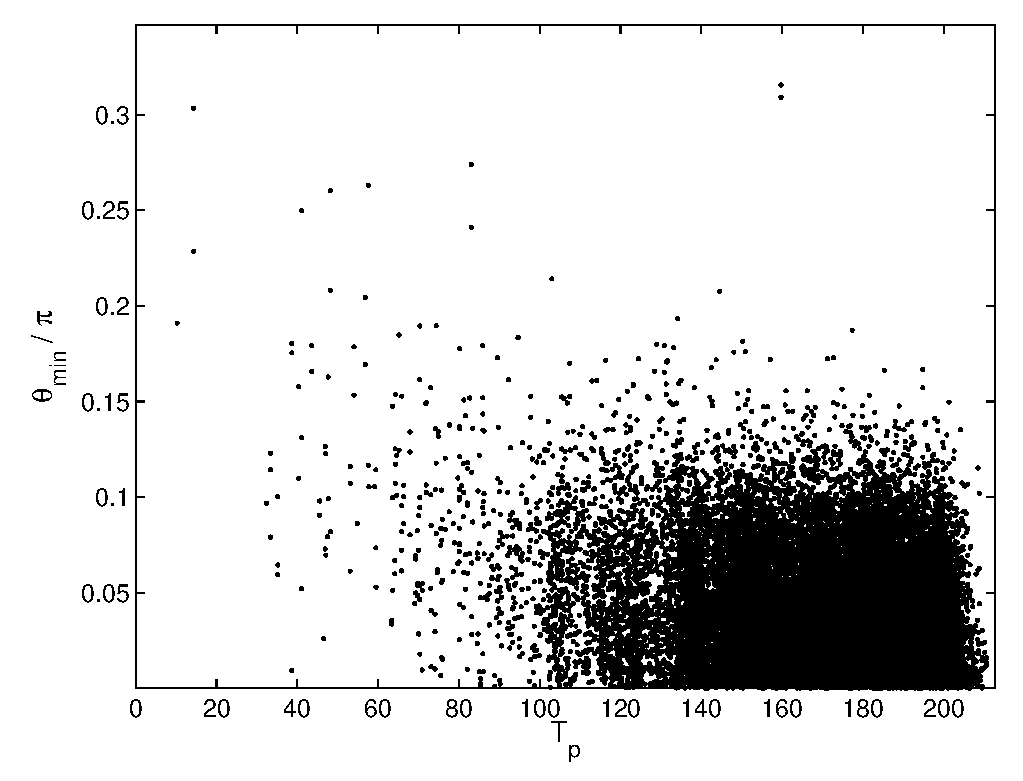
\includegraphics[width=0.44\textwidth]{ks22ppo_min_angle}
    ~(b)\includegraphics[width=0.44\textwidth]{ks22ppo_min_angle_floq}\\
    (c)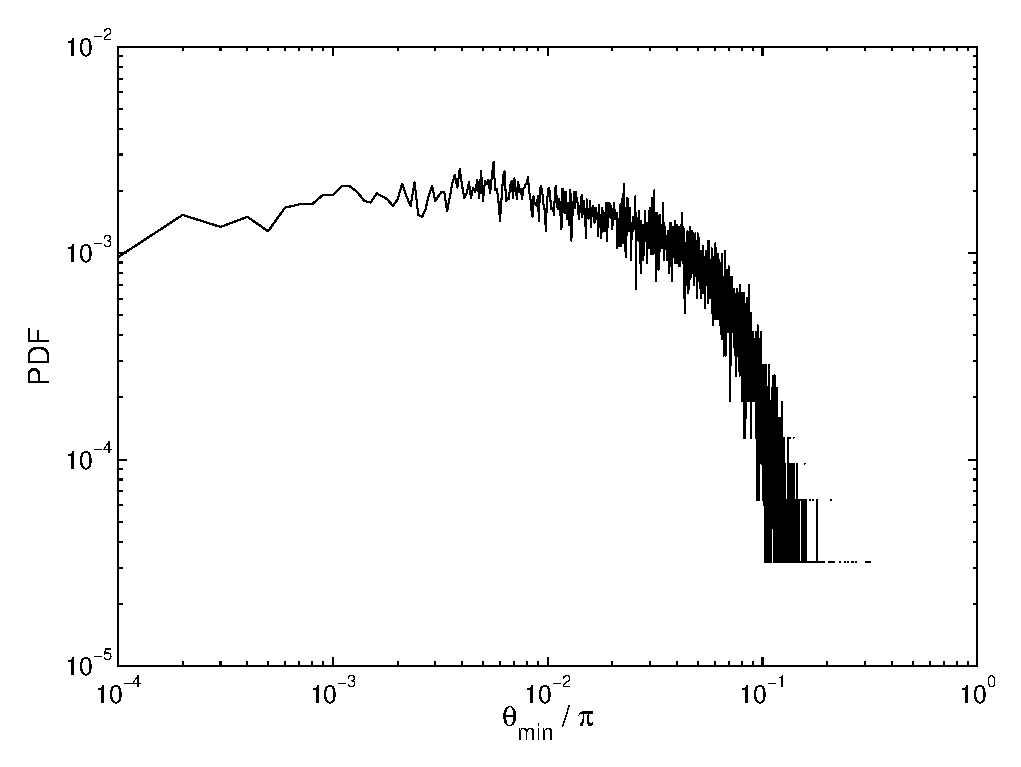
\includegraphics[width=0.47\textwidth]{ks22ppo_min_angle_pdf}
    \caption{
      Approximate minimum angle of pairs of Floquet eigenvectors
      $\jEigvec[i],\, \jEigvec[j]$, $i,j=1,\ldots 5,\, i\neq j$ (angle was not
      computed for marginal directions) along numerically computed points of
      periodic orbits, (a) versus the period of the orbit $T_p$. Red solid line
      shows the average minimum angle over bins of $\Delta T_p=15$. (b)
      Minimum angle versus the largest Floquet exponent $\eigRe[1]_p$.
      (c) Probability density function of the minimum angles shown in panel
      (a). KS system size $L=22$, 16 Fourier modes truncation.
    }
    \label{fig:ks22ppo_min_angle}
  \end{figure}
  %%%%%%%%%%%%%%%%%%%%%%%%%%%%%%%%%%%%%%%%%%%%%%%%%%%%%%% 


\item[2011-10-26 Evangelos]
  I've looked at the minimum angles of pairs of leading Floquet vectors
  across all periodic orbits (not relative periodic) in Ruslan's data. I
  could reliably get the first five Floquet vectors for about $10,000$
  orbits with periods $T\in[10.25, 210.61]$ out of approximately $30,000$
  orbits in the set. Results are shown in \reffig{fig:ks22ppo_min_angle}.
  Largest (minimum) angle detected was $0.3155\pi$, smallest one was
  $3\times10^{-7}\pi$.

\item[2011-10-26 Predrag] \refFig{fig:ks22ppo_min_angle} is really
  interesting. Plotting the angle {\em vs} the leading Floquet exponent $\eigRe[1]_p$
  rather than time \period{p} is probably more informative.


  The \po s are not really \po s (there are none in the
  antisymmetric subspace for $L=22$, right?), but these pre-periodic
  things that drift in the group tangent direction and then return? [{\bf ES}: yes]
  You are using right (expanding forward in time) Floquet eigenvectors
  $\jEigvec[i]$? [{\bf ES}: yes] Maybe for contracting directions one has to switch to the
  left Floquet eigenvectors $\jEigvecT[i]$. Hugues will know.
  [{\bf ES 2011-10-27}: Just to be clear about what I do compute: I use the Jacobian
  calculated over a complete period ($2T_p$) to compute Floquet eigenvectors.
  Any objection? {\bf PC 2011-10-27}: dunno...]

  You are right to ignore the marginal directions, but it might be that
  when you do it correctly (\Poincare\ in time direction, \slice\ in \SOn{2}
  direction) you will get much larger angles, as $\jEigvec[i]$ might form
  very non-normal narrow pencils of eigenvectors, stretched out along the
  flow direction.

  I only have H\'enon intuition, not sure how it will play out for higher
  dimensions. If my hunch is right, I think for starters you should select
  only the \po s for which the leading pair $\jEigvec[1] \cdot \jEigvec[2]$
  has a small smallest angle, and then plot the point on the cycle where
  the angle is smallest, projected on $3D$ a physical coordinate
  frame\rf{GHCW07,SCD07} (no Fourier mode projections, please). It really
  should be plotted in a \Poincare\ in time direction, \slice in \SOn{2}
  direction, but we have not gotten that far. Note also that this $\cdot$
  product has no invariant meaning, the eigenframe is not orthogonal.

  If we are lucky these points
  will align, telling us where the primary folds (in the sense of H\'enon
  pruning front theory, \refchap{c-Henon}). But probably that will happen
  only in a {\PoincSec}, in the full flow the folds in unstable
  manifold have an extra, longitudinal dimension, which makes them a hell
  to visualize. Ditto the \SOn{2} tangent AKA drift direction.

  Once we see where these folds are in the \statesp\ we'll think of less
  painful ways of nailing them down then by the close \po\ passages.

  Small angles in $\jEigvec[2] \cdot \jEigvec[3]$, \etc, have to do with
  `non-leading' folds in the less expanding unstable manifold directions,
  so they will be trickier to visualize. Guys who generalize baker maps to
  volumes call that 'hyperchaos'. I have not been able to visualize these
  higher-dimensional folds. Again, just my pruning front hunch, might play
  out differently when there are 8 physical dimensions.

\item[2011-10-26 Predrag] Note that the leading Lyapunov exponent is
  $\Lyap = 0.048$ (see {\bf [2009-09-13 Ruslan]} above), and all
  $\eigRe[1]_p \geq 0.024$ in \reffig{fig:ks22ppo_min_angle}\,(b), so there
  could be a square-root non-hyperbolicity, indicated by families of cycles
  $\eigRe[1]_p \to \Lyap/2$, as in Fig 2  of \refref{AACII}, click
  \HREF{http://www.cns.gatech.edu/~predrag/papers/AAC-II.pdf}{here}.

\item[2011-11-01 Evangelos] Hugues was in Chemnitz, talked with Yang and Radons.
  Yang claims he can determine the dimension of the ``inertial manifold'' for
  KSe $L=38.5$ in antisymmetric subspace (as in Lan and Cvitanovi\'c\rf{lanCvit07})
  simply by counting the number and dimensions of hetero- and homoclinic connections of
  equilibria in the system. However, he failed to explain to Hugues how he does it.

\item[2011-11-01 Evangelos and Hugues 2 Predrag] We think this might not be a totally
  crazy idea, but we are unsure whether it could be applied to larger systems (or in the
  full space).

  If we assume dynamics live on a finite dimensional space of (unknown)
  dimension $D$, then a robust connection will occur if the dimension
  $d_u^{(1)}$ of the unstable manifold of the ``donor'' \EQV{1} and the
  dimension $d_s^{(2)}$ of the stable manifold of the ``receiver''  \EQV{2}
  obey $d_u^{(1)}+d_s^{(2)} \geq D+1$ (this is just the condition for
  transversal intersection of $d_u^{(1)}$- and $d_s^{(2)}$-dimensional
  manifolds in $D$-dimensional space). % Since $d_s^{(2)}=D-d_u^{(2)}$ %
  (where $d_u^{(2)}$ the dimension of the stable manifold of the receiver)
  we get $d_u^{(1)}-d_u^{(2)}\geq1$. We know $d_u^{(1)}$ and % we can
  estimate $d_s^{(2)}=\sum_i d_u^{(i)}$ where $i$ runs over all known %
  ``donors'' from which a connection to \EQV{2} exists? we need an estimate
  for  $d_s^{(2)}$ in order to bound D from above. Presumably this is what
  Yang computes by taking into account the dimensions of all incoming
  unstable manifolds into \EQV{2}, but we do not know any details.

\item[2011-11-03 Predrag] I always have to think this argument through -
  not quite sure it is right. Maybe this helps -
  clippings from \refref{GHCV08}: ``
  Our computations rely on the simple principle that an object of dimension
  $k$ is likely to intersect in a stable way an object whose codimension in
  {\statesp} is less than or equal to $k$. At the bottom, this is nothing
  more than the fact that two submanifolds in general position can
  intersect if the sum of their dimensions is greater than or equal to the
  dimension of the {\statesp} (whether they actually intersect is a subtle
  question that is central to the ``structural stability'' of chaotic
  dynamical systems\rf{smale}). For an illustration in the nonlinear
  setting, see \refref{AbSh92}. Kevrekidis \etal\rf{KNSks90} (see Section 5
  of their paper) make elegant use of this principle and of invariant
  subspaces implied by discrete symmetries of the underlying PDE to
  numerically deduce the existence of a heteroclinic connection in the
  Kuramoto-Sivashinsky equation. Indeed, they comment that their work may
  have implications for shear flows. With regard to the heteroclinic
  connections presented here, it is significant to note from Table~1 that
  the codimension of the stable manifold in the $S$-invariant space (which
  is equal to $d(W^u_S)$) of $\tLB$ is less than the value of $d(W^u_S)$
  for $\EQV{i}$ with $i=3,4,5$. Thus it is not surprising that the unstable
  manifolds of $\EQV{i}$ with $i=3,4,5$ intersect the stable manifold of
  {$\tLB$} in a stable way (\ie, robustly with respect to small changes of
  system parameters).
  ''

  Are you guys saying ``two submanifolds can intersect if the sum of their
  dimensions is greater than or equal to the dimension of the {\statesp}'',
  \ie,
  \beq
  d(W^u_{(1)})+d(W^s_{(2)}) \geq d\,,\quad \mbox{or }
  d(W^u_{(1)}) \geq d-d(W^s_{(2)})
  \,?
  \ee{hecsRobust}
  That argument does not require invoking the 'physical' dimension $D$, all
  unphysical dimensions are subtracted equally from $ d$ and $d(W^s_{(2)})$.

\item[2008-04-10 Predrag]
  This received wisdom that heteroclinic connections are due to
  continuous symmetries is nonsense. You have a heteroclinic connection
  in Lorentz, right? They can be robust if dimension of unstable
  manifold A + codimension of the stable manifold B add to or exceed
  the dimension of the \statesp, as explained in \refref{GHCV08}.

\item[2011-11-03 Predrag] By the way, it is not obvious to me that each local
  chart of a good atlas of the inertial manifold has the same physical dimension?
  Maybe there is some transitivity argument that it has to be so for all
  charts belonging to the same ergodic set. I do not know.

\item[2011-11-01 Evangelos and Hugues]
  We would also consider natural to take into account hetero- and
  homoclinic connections of (relative) periodic orbits, eventually building
  a network of interconnected invariant objects. Could we tell the
  dimension of the ``inertial manifold'' simply by counting vertices in
  this network? It would be natural to weight nodes in this network by
  their relative importance [as estimated by either their stability or by
  the number of times they are found in Ruslan's random search (these are
  known)], so that we preferentially examine connections of the most
  important nodes.

  How does this sound?

\item[2011-11-01 Ruslan] I suggest to weigh by stability, rather than
  the number of times found, since, even though the two are correlated, the
  latter also reflects the properties of the search algorithm, which you
  don't need in your analysis.

\item[2011-11-04 Predrag] I fully agree with Ruslan - I do not know of
  any argument that would identify a basin of attraction of the search
  method (small for Newton, large for variational methods described in
  ChaosBook.org ``Relaxation for cyclists'') with the natural measure of
  the same, given by its `geometrical' cycle stability and period weight.
  In our \pCf\ papers Gibson has used the frequency of how often a cycle
  shows up in searches that take initial point as a coarse measure of its
  weight, but that is because we have nothing better - we have no
  systematic symbolic dynamics and no systematic way of uniformly
  populating the strange attractor with cycle points in that case.

\item[2011-11-01 Evangelos and Hugues 2 Ruslan] We thought that if the
  trajectory Ruslan used to fish for relative periodic orbits is still
  available, and if the association of each located orbit to the point on
  the trajectory used as an initial guess is still known, we might have a
  quick and dirty way to figure out which connections of relative periodic
  orbits might be present and preferentially visited (follow how the
  chaotic trajectory hops from the neighborhood of one orbit to another).
  Are any data of this kind still available?

\item[2011-11-01 Ruslan] No, because I didn't use a single trajectory,
  but rather random initial conditions within a rectangular region of
  Fourier space containing the attractor, as described on p. 30 of
  \refref{SCD07}. If you want to find such a network of RPOs/PPOs, then I would
  suggest to generate a 'typical' long chaotic orbit and run a 'proximity'
  search on it.  I have attempted it some time ago and briefly described
  the results in my Snowbird 2007 presentation (see
  siminos/rpo\_ks/davidchack/DS07.ppt slides 28-31).  I believe this is
  something similar to what Kazz is doing (in terms of minimizing the
  distance along time a phase).  By the way, the same proximity search can
  be carried out among the RPOs/PPOs themselves. I'm sure this will allow
  us to organize them into 'happy families'.

\item[2011-11-02 Evangelos] A ``proximity'' search among RPOs/PPOs is
  what I am running right now with the goal of simply finding orbits close
  to the shortest periodic orbit. However, organizing the orbits into
  families this way really seems possible now. Stay tuned...

\item[2011-11-04 Ruslan] Just to point out that there is a caveat when
  looking at the proximity between RPOs/PPOs.  The proximity of a chaotic
  orbit to RPOs/PPOs gives the true picture of the influence of the latter
  on the orbit. But proximity between RPOs/PPOs (in the way we define it)
  is only an approximation to such influence, because it might happen that
  the phases of the two nearby RPOs/PPOs are not linked dynamically (i.e.
  they are not on the same slice).  But I suspect that RPOs/PPOs in very
  close proximity will have phases from nearby slices, hence I call it an
  'approximation'.

\item[2011-11-02 Evangelos] Asked by Hugues to plot the average minimum
  angle over some bins in $T_p$ in \reffig{fig:ks22ppo_min_angle}(a). I
  think it shows a tendency towards smaller angles for larger periods, but
  I wouldn't be able to say for sure whether it saturates towards some
  finite value or tends to zero. However, given the fact that we sample
  over a finite set of points along each orbit, so a tendency of the
  minimum angle towards a finite value should be expected.

\item[2011-11-04  Hong-Liu Yang]
  
  How is your reading of our preprint? Comments and suggestions are indeed welcome.

  Now I come back to your question posed at Paris that giving the \po s, as
  many as one wants, could one get the dimension of inertial manifold (IM)
  from those \po s?

  I got an idea to address this issue and think the answer should be yes.
  For the case of 1D KSe with L=22, one can already get the IM dimension 9
  from the information provided in your SIAM 2010 paper.

  It is known that \po s have different numbers of unstable directions,
  normally less than the IM dimension. From our previous {\cLv} analysis of
  IMs, we know that some stable directions should also take part in the
  dynamics on IMs. For \po s the number of stable directions are infinite,
  then the essential point is which stable directions should be included.
  The decision can not be made from the local stability information of \po
  s, like the Floquet exponents or vectors as you know already. We do need
  some global information, the heteroclinic connections. Heteroclinic
  connections go from the unstable directions of one \po  to the stable
  directions of another \po. A network can thus be formed with \po s as the
  nodes and heteroclinic connections as the links. Each node has both
  outcoming links (unstable directions) and incoming links (stable
  directions). For a given \po  the stable directions (incoming links) are
  historically unstable as the trajectory is close to the \po  at the other
  end of the heteroclinic connections. These stable directions should thus
  take part in the IM dynamics. Then one can simply count the number of
  total links of a give node to get the local estimate of the IM dimension.
  For a complete network, the ideal case, one can get the IM dimension from
  any representative nodes/\po s. Since the number of \po s is infinite, in
  general we can only start from "important" \po s to form a partial
  network and get the maximal value of the node-wise estimates. As we
  increase the number of nodes gradually the maximal estimate is expected
  to saturate to the (unknown) IM dimension when the network becomes
  sufficiently representative.

  Actually I would say the proposed network picture of chaos is the general
  organization rule of \po s for systems with or without IM.

  We should also say that this is not the only way of the organization of
  stable and unstable directions in a chaotic attractor, see for instance
  the Smale horseshoe picture. Possibly, hyperbolic and nonhyperbolic
  system have the different ways of organization.

  One possible concern could be the genericity of the occurrence of
  heteroclinic connections. My guess is that \po s are inter-connected as
  they are created via bifurcations. These inter-connections persist even
  when the system is away from the bifurcations. The existing connection
  can also be changed or destroyed when a new bifurcation occurs.

  Another issue, raised by Guenter, will be whether a partial network
  formed by only the equilibria can already give us the correct IM
  dimension, like the case of KSe with $L=22$. If so, the task can be greatly
  simplified.

\item[2011-11-07 Kazz] Can I have your raw data for \reffig{fig:ks22ppo_min_angle}.
  Comparing the orbits in the figure and those I studied in the PRL-style draft,
  Hugues and I agreed that the orbits we studied are actually not so typical;
  their period is too short and they are among the most hyperbolic ones.
  We should therefore look also at more typical orbits.
  For this purpose, I'd like to have your list of orbits with their period,
  degree of hyperbolicity, and the value of the first Floquet multiplier, i.e.,
  the raw data for \reffig{fig:ks22ppo_min_angle}.

  I'm also curious how things go on your side, in the attempt to measure
  the relation between the difference vector and the physical subspace
  for the collection of orbits.

\item[2011-11-07 Evangelos] Apart from the reasons you mention above,
  I also think you should look at other periodic orbits because I've
  had difficulties identifying relatively short periodic orbits that visit
  the neighborhood of \PO{10.25}.

  I've been looking at close encounters of periodic (and relative periodic) orbits
  in order to study the angle of the difference vector and the subspace spanned
  by the $n$ first Floquet eigenvectors.

  Some interesting examples are given in \reffig{fig:ks22shad} (see caption).
  In particular \PO{32.36} appears to shadow quite a few longer orbits.

  \begin{figure}% [ht]
    \begin{center}
      (a)\includegraphics[width=0.45\textwidth]{ks22ppoT10235shad.png}~
      (b)\includegraphics[width=0.45\textwidth]{ks22ppoT7035shad.png}\\
      (c)\includegraphics[width=0.45\textwidth]{ks22ppoT10235angl_dist.png}~
      (d)\includegraphics[width=0.45\textwidth]{ks22ppoT7035angl_dist.png}
    \end{center}
    \caption{Shadowing of periodic orbits. (a) Hyperbolic pre-periodic orbits
      \PO{32.36} and \PO{40.35} shadow \PO{102.4} which appears to be close
      to non-hyperbolicity. Note that \PO{102.4} traces \PO{32.36} twice.
      (b) \PO{70.35}, is shadowed by \RPO{34.64} and \RPO{39.77}.
      (c) Angle of first two Floquet eigenvectors along \PO{102.4} (red, solid line) and
      closest distance from \PO{102.4} of points on \PO{32.36} (blue triangles) and \PO{40.35}
      (green crosses). (d) Angle of first two Floquet eigenvectors along \PO{70.45} (red, solid line) and
      closest distance from \RPO{70.45} of points on \PO{34.64} (blue triangles) and \RPO{39.77}
      (green crosses).
    }
    \label{fig:ks22shad}
  \end{figure}

  \begin{table}[h!]
    \caption{ Period $T_p$, shift $\shift_p$, leading (non marginal) Floquer multipliers $\ExpaEig_{p,i}$,
      corresponding exponents $\eigRe[p, i]$ and minimum angle of first two (non marginal) Floquet
      eigenvectors for each orbit.	
    }\label{tab:ks22shad}
    \begin{center}
      \begin{tabular}{ccccrrc}
        $T_p$  & $\shift_p$  & $\ExpaEig_{p,1}$ & $\ExpaEig_{p,2}$ & \eigRe[p, 1] & \eigRe[p, 2] & $\theta_{1,2}/\pi$  \\\hline
        32.36 &-- &  $-45.4\pm 47.9i$ & $1.19\times 10^{-5}$  &  0.0647 &  -0.1751 & 0.1 \\
        40.35 &-- &  $1.12\times 10^8$ & $2.34\times 10^{-3}$ &  0.2297 &  -0.0750 &  0.1\\
        102.4 &-- &  $1.29\times 10^9$ & $6.10\times 10^4$  &  0.1025 &   0.0538 & 0.005\\\hline
        34.64 & 9.600 & 35.8 & 31.6  &   0.0516  &  0.0498  & -- \\
        39.77 & 1.611 & $2.73\times 10^4$ & 0.441 & 0.128 &  -0.0103 & --\\
        70.35 & -- & $2.61\times 10^4$ & $3.51\times 10^2$ & 0.0742 &   0.0417 & 0.02\\\hline
        38.66 &-- & $2.36\times 10^3$ & $4.96$ & & & 0.01
      \end{tabular}
    \end{center}
  \end{table}

  In order to find such close encounters efficiently I first tried some
  rudimentary slicing but encountered problems with jumps as described
  elsewhere\rf{SiCvi10,FrCv11}. So I've settled with using $\On{2}$-invariant
  variables similar in spirit to the ones in my thesis\rf{SiminosThesis}
  but given in a compact form without the use of computer algebra. I've noted
  down the expressions in siminos/ksReduced, in case you would like to know what
  is plotted in \reffig{fig:ks22shad}. I also suggest using these transformations
  when looking for close encounters of chaotic trajectories with periodic orbits.

  I now intent to turn to the actual computation of the angle of the difference
  vector and the subspace spanned by the $n$ first Floquet eigenvectors. However,
  I think I cannot get more than 6 (including marginal) eigenvectors accurately
  enough to draw safe conclusions. If I am correct, then the only option would be
  to send to Kazz some initial conditions for periodic orbits which come close
  to a reference orbit, so that he can get the vectors with better accuracy.

  Kazz, I'd also like to send you initial condition for \PO{38.66} anyway, to
  see if you can verify the angle between Floquet eigenvectors being small.

  % \item[2011-11-07 Kazz] Regarding svn, I have the updated source files,
  %   but I cannot compile the tex. It seems that many latex style files are missing.
  %   I found them by myself, but it doesn't work probably because of the version mismatch...
  %   
  % \item[2011-11-07 Evangelos] No can help... sorry. I haven't used Windows for
  %   anything serious for too many years. Maybe Predrag knows?
  %   
  %   Predrag helped fixed this, OK now.

\item[2011-11-9 Evangelos] Note updated \reffig{fig:ks22shad} and \reftab{tab:ks22shad}.

\item[2011-11-9 Evangelos] There seems to be an unstable manifold variability argument
  emerging from \reffig{fig:ks22shad} and \reftab{tab:ks22shad}. Periodic orbits
  \PO{32.36} and \PO{40.35} are hyperbolic with unstable manifolds of dimension $1$ and $2$
  respectively. They appear to shadow \PO{102.4} which has a $2-$dimensional unstable manifold
  and small minimum angle of the two unstable eigenvectors, \ie\ it would appear
  to be non-hyperbolic. In the same manner, \RPO{34.64} and \RPO{39.77} with unstable manifolds
  of dimension $1$ and $2$, respectively, shadow \PO{70.35}, which has $2$-dimensional
  unstable manifold and is non-hyperbolic (I haven't computed minimum angle of eigenvectors
  for \rpo s yet).

  Note that \PO{38.66}(not plotted) shadows \RPO{34.64}. It would be interesting to look
  at this from a (dynamical) symmetry breaking bifurcation perspective.

\item[2011-11-9 Evangelos]  In all cases shown here,
  the periods of the shorter cycles (multiplied by the number of times a cycle is revisited)
  (approximately) add up to the period of the longer cycle shadowed by the short ones.
  I don't know whether we should read too much into \rpo\ shifts adding up to zero (or $L/2$)
  when two \rpo s shadow a \po.

\item[2011-11-07 Hugues] The data of \reffig{fig:ks22shad} would be nice,
  but what we would need also are the full coordinates of some selected orbits with:
  \begin{itemize}
  \item not-so-large period
  \item very small minimum angle
  \item preferably first Floquet exponent near the first stability exponent
  \end{itemize}

  From \reffig{fig:ks22shad}, we can see that there are certainly some like
  that with a period near 80, and probably some not so bad with period around 40...


\item[2011-11-9 Evangelos] I think the two longer orbits in
  \reftab{tab:ks22shad} are good candidates (although Floquet exponent is
  not very close to the first Lyapunov exponent) for Kazz to repeat the
  calculations in his draft. I will study them in more detail anyway, to
  see where the angle of eigenvectors becomes minimal, \etc.

\item[2011-11-15 Evangelos] Updated \reffig{fig:ks22shad}. For each of
  the numerically computed points along each of the shorter cycles we plot
  the minimum distance from any of the numerically computed points along
  the longer cycle to which they come close. We also plot the angle
  $\theta_{1,2}$ of the unstable Floquet eigenvectors along the points of
  the longer cycle. For both cases shown in \reffig{fig:ks22shad}, we
  observe that (local) minima of $\theta_{1,2}$ are associated with passage
  from the neighborhood of one of the shorter cycles to the neighborhood of
  the other. For instance, in \reffig{fig:ks22shad}(d) we can see that
  points on \PO{70.45} which are close to \RPO{34.64} are separated by
  points close to \RPO{39.77} by the global minimum of $\theta_{1,2}$ at
  $t\simeq37$, while a local minimum at $t\simeq70$ is associated to
  passage from the neighborhood of \RPO{39.77} to that of \RPO{34.64}.

\item[2011-11-15 Predrag] (a very minor suggestion) - I guess your angle
  is always positive, so why not plot $(t,\ln \theta_{1,2}(t))$ - it will
  emphasize the close passages, which is what you care about.
  {\bf 2011-11-16 Evangelos} Both distances and angles are already plotted
  in logarithmic scale to emphasize close passages.
  {\bf 2011-11-16 Predrag}
  Sorry, I see that the right edge of \reffig{fig:ks22shad}\,(c) is logarithmic
  but I guess I do not understand the left edge - shouldn't 0.1, 0.01 and 0.001
  be equally spaced? {\bf 2012-05-21 Evangelos} Sorry, it is fixed now.
  (It ways very quirky to do it correctly. It seems matlab refuses to
  plot both axes in log scale in a straitforward manner,
  or it's just that I've learned it after 30.)

\item[2012-02-06 Evangelos] Talked with Hugues at MPIPKS, created a to-do list:
  \begin{itemize}
  \item Compute ``IM'' dimension from periodic orbits only:
    \begin{itemize}
    \item
      Compute difference vector of points of closest approach of two
      nearby periodic orbits. Compute Floquet vectors of periodic
      orbits. Proceed as in Takeuchi and Chat\'e draft to infer
      dimension of ``IM''.
    \item
      Find bits of trajectory shadowing two short periodic orbits (and
      possibly a third longer one which shadows the two short orbits),
      compute dimension of ``IM'' as in Takeuchi and Chat'e draft.
      Compare with dimension we get from periodic orbits alone.
    \end{itemize}
  \item Tangencies of trajectory and proximity of ``non-hyperbolic'' \po s.
    \begin{itemize}
    \item
      Choose a collection of typical periodic orbits (\ie\ with leading
      Floquet exponent close to the leading stability exponent of the flow)
      with small minimum angle of Floquet eigenvectors. Calculate
      systematically distance of chaotic trajectory to all of these.
    \item
      Is there a correlation between tangencies and proximity to one of
      these \po s?
    \end{itemize}
  \end{itemize}

\item[2012-02-14 PC]                        \toCB
  As almost no \po s are stable, I call unstable \po s simply '\po s,' and
  the stable ones 'limit cycles'. `UPOs' is a Maryland abomination,
  aesthetically. But we have a more important nomenclature decision to
  make: for dynamical systems with $\SOn{n}$ symmetry there are generically
  no \po s, only \rpo s. In presence of discrete symmetries there are \po s
  in the invariant subspaces fixed by discrete symmetry subgroups, but they
  have no relation to the chaotic / turbulent dynamics (compare
  Christiansen\rf{Christiansen97} with Cvitanovi{\'c}, Davidchack, and
  Siminos\rf{SCD07}). In the above you keep talking about \po s, but the
  chaotic dynamics is supported by \rpo s and pre-periodic \rpo s, 50-50\%,
  no \po s at all. From \refref{SCD07}:

  ``Due to invariance under reflections, KS equation can also have
  \rpo s {\em with reflection}, which are
  characterized by a profile $u_p(x)$ and
  period $\period{p}$
  \beq
  \Refl u(x+\shift,\period{p}) =
  -u(-x-\shift,\period{p}) = u(x+\shift,0) = u_p(x)
  \,,
  \label{KSpos}
  \eeq
  giving the family of equivalent solutions
  parameterized by $\shift$
  (as the choice of the reflection point is arbitrary,
  the shift can take any value in $-L/2 < \shift \leq L/2$).

  Case {\bf (b)}: The \po\ satisfies
  \beq
  u(x,t+\period{p})=\gamma u(x,t)\,,
  \label{eq:POspattemp}
  \eeq
  for some group element $\gamma\in \On{2}$ such that $\gamma^m=e$ for some
  integer $m$ so that the orbit repeats after time $m \period{p}$ (see
  \refref{golubitsky2002sp} for a general discussion of conditions on the
  symmetry of \po s). If an orbit is of reflection type \refeq{KSpos},
  $\Refl\Shift_{\shift/L} u(x,\period{p}) = -u(-x-\shift,\period{p}) =
  u(x,0)$, then it is pre-periodic to a \po\ with period $2\period{p}$.
  Indeed, since $(\Refl\Shift_{\shift/L})^2 = \Refl^2 = 1$, and the KS
  solutions are time translation invariant, it follows from \refeq{KSpos}
  that
  \[
    u(x,2\period{p}) = \Refl\Shift_{\shift/L} u(x,\period{p}) =
    (\Refl\Shift_{\shift/L})^2 u(x,0) = u(x,0)\;.
  \]
  Thus any shift acquired during time $0$ to $\period{p}$ is compensated by
  the opposite shift during evolution from $\period{p}$ to $2 \period{p}$.
  All periodic orbits we have found for $L=22$ are of type
  \refeq{eq:POspattemp} with $\gamma=R$. Pre-periodic orbits with
  $\gamma\in C_n$ have been found by Brown and Kevrekidis\rf{BrKevr96} for
  KS system sizes larger than ours, but we have not found any for $L=22$.
  ''

  In the rest of the paper we call \po s of type \refeq{eq:POspattemp} with
  $\gamma=R$ `pre-periodic.' We should give them their own name (or find
  one in the literature?), reserve `pre-periodic' for the $\gamma\in C_n$:
  those are truly periodic on the fundamental domain that is $1/n$ of the
  full \statesp, see ChaosBook.org chapter
  ``\HREF{http://chaosbook.org/paper.shtml\#discrete}{World in a mirror},''
  where \Rot{1/2} case is worked out in detail for the one-eared Van Gogh
  attractor.

\item[2011-12-06, 2012-02-14 PC]
  I tried out the word ``inertial manifold'' [IM] (invariant and exponentially
  attracting) on a few mathematicians, and they get very worked up - it is
  not defined, it has been shown that it cannot be defined in 3 dimensions
  (million dollar question) \etc. In particular, we have to work on
  convincing Constantin that this is new - he sees nothing new in the
  {\cLvs} approach, believes they did it all much earlier in their
  proof of the finite dimension of the KS ``global attractor'' (I believe
  that is what they call it, not ``inertial manifold''. It is a million
  dollar question. We should recheck the literature -
  \refref{constantin_integral_1989,Constantin97} and a number of other
  papers (read {\bf [2011-07-25 PC: Inertial manifold literature]} in
  \refchap{s:LyapunovVec}). He is smart and highly regarded in the
  mathematics community, so we definitely do not want to have him dismiss
  this work.

  Tentative suggestion: perhaps safer to say ``global attractor'' or
  ``{\nws}''. Though neither is what we have in mind (it has to be a
  connected, transitive attractor).

\item[2012-02-14 PC] I still do not know whether partially hyperbolic
  invariant tori (such as computed in \refref{LCC06}, provided they really exist)
  are more important than \rpo s in supporting shmurbulence on attractors whose
  physical dimension is of order 10-1000...

\item[2012-02-06 Evangelos]
  It also seems I will eventually need to implement the {\cLv}
  calculation algorithm of Ginelli \etal\rf{ginelli-2007-99}. I will
  ``officially'' have more time in March, but I am a
  \HREF{http://www.structuredprocrastination.com/}{structured
    procrastinator} so I might actually turn to this right now.
  {\bf [2012-02-14 PC]} Sara ordered me to read this months ago, but
  I'm procrastinating.

\item[2012-03-15 Kazz]
  Maybe I should add here some words in relation to Constantin's understanding.
  First, showing the finite dimensionality of the inertial manifold
  or the global attractor, which was indeed proved mathematically
  for systems like KS,
  is not the central point of our {\cLv} approach.
  Instead, we gave an \textit{exact} number for this dimension,
  albeit not rigorously, whereas the mathematicians could provide
  only its upper bound which does not look ``physical'' at all;
  for example, the best upper bound for the KS inertial manifold dimension
  so far is $\text{const.} \times L^{2.46}$, while we naturally expect it
  to be proportional to $L$ for the extensivity.
  I completely agree that we should try to convince him of this point,
  all the more because we need help of mathematicians like him to establish
  the bridge between our {\cLv} approach and the inertial manifold
  on firm grounds.

  Concerning the inertial manifold vs global attractor, as far as I
  understand, the former is a smooth invariant manifold of integer
  dimension that attracts outside trajectories exponentially, while the
  latter is a manifold of finite Hausdorff (thus noninteger) dimension in
  which trajectories are confined after infinitely long time.
  We believe that what we see by {\cLvs} is the former,
  because of the integer dimension and the exponential attraction.

\item[2012-03-15 Predrag] I agree, Constantin bounds ``the global
  attractor of the dissipative system.'' This is a fragile object, and
  can easily change non-smoothly as you vary things like $L$. If
  `inertial manifold' is what you say, we also need some statement that
  the integers they get are the best possible and agree with your (sharp)
  physical dimension.

  In my humble opinion Hausdorff and other `fractal' dimensions are
  useless, while your 'physical' integer dimension is the best thing since
  invention of Swiss cheese. Convergence of Fourier series for KS makes
  more physical sense to me. We have written this in \refref{SCD07}:

  ``
  In the Fourier basis the conservation of energy on average takes form
  \beq
  0 = \sum_{k=-\infty}^{\infty} ( q_k^2 - q_k^4 )\,
  \timeAver{E}_k
  \,,\qquad
  E_k(t) =  {\textstyle\frac{1}{2}} |a_k(t)|^2
  \,.
  \ee{EFourier1}
  The large $k$ convergence of this series is insensitive to the system
  size $L$; $\timeAver{E_k}$ have to decrease much faster than $q_k^{-4}$.
  Deviation of $E_k$ from this bound for small $k$ determines the active
  modes. For \eqva\ the $L$-independent bound on $E$ is given by
  Michaelson\rf{Mks86}. The best current bound\rf{GiacoOtto05,bronski2005}
  on the long-time limit of $E$ as a function of the system size $L$ scales
  as $E \propto L^{2}$.
  ''

  Forever it is worth, here are my notes (June 2008) cribbed from
  Bronski\rf{bronski2005} and/or talking to people:

  ``
  Nicolaenko, Scheurer and Temam\rf{NSTks85} gave the first long-time
  boundedness result for the Kuramoto-Sivashinsky equation, showing that
  $\limsup_{t \rightarrow \infty} |\!|u|\!|_2 \le C L^{\frac{5}{2}}$ for
  odd initial data, as well as showing that bounds on the $L_2$ norm imply
  bounds on the dimension of the attractor.

  The $L_2$ estimate was improved by Collet, Eckmann, Epstein and
  Stubbe\rf{CEEksgl93} who  extended it to any mean-zero initial data and
  improved the exponent from $\frac{5}{2}$ to $\frac{8}{5}$, and by
  Goodman\rf{Good94}, who extended it to any mean-zero initial data with the
  same exponent.

  In these papers the function $|\!|u-\phi|\!|_2^2$ is a Lyapunov function
  for an appropriately chosen $\phi$ and $|\!|u|\!|_2$ sufficiently large.

  Bounds which do not fit into Lyapunov function framework:
  Ilyashenko\rf{Ilyash92}, Otto  and Giacomelli\rf{GiacoOtto05}. The
  latter, which treats the KS equation as a perturbation of the Burger's
  equation, is currently the best estimate, establishing that
  \[
    \limsup_{t \rightarrow \infty} |\!|u|\!|_2 = o(L^{\frac{3}{2}}).
  \]
  Bronski and Gambill\rf{bronski2005} give an argument of the Lyapunov
  function type which establishes the slightly weaker result
  \[
    \limsup_{t \rightarrow \infty} |\!|u|\!|_2 = O(L^{\frac{3}{2}}).
  \]
  Their proof applies equally to the destabilized \KSe
  \[
    u_t = -u_{xxxx} - u_{xx} + \gamma  u + u u_x
    ~~~~~~\gamma > 0 ~~~~~ \int u(x,0)dx = 0.
  \]
  It was shown by Wittenberg\rf{Witte02} that this equation
  has stationary solutions which satisfy $|\!|u|\!| \propto L^{\frac{3}{2}}.$
  Since a Lyapunov function argument for the KS equation also applies
  to the dKS equation (for sufficiently small $\gamma$) Wittenberg
  argued that $\frac{3}{2}$ is the best exponent that one can expect
  from the Lyapunov function approach.

  Similar ideas of greater generality have been used by Constantin and
  Doering\rf{CoDoe92,CoDoe95} to establish bounds on energy dissipation in
  fluids, and generally go by the name `background flow method.'

  % 
  {\bf PC}:
  % Past: Michael Loss has not taught us how to bound $E$ by
  % Sobolev bounds. Neither has Spiegel. Next: But
  Constantin says that the answer is in \refrefs{NSTks85}. Eckmann says:
  the  best bound is by Otto\rf{GiacoOtto05}; the only bound close to $k=0$,
  better in essential way. Eckmann had
  $L^{8/5}$, but conceptually Otto is the best. Recheck whether it is $|u|$
  or $E \propto L^{3/2}$. When the solution is big, how long can it stay
  big? They found it cannot stay big for long.

  Predrag: From bounds on energy, we might be able to bound the number of \eqva\ as
  function of systems size $L$, and thus be sure we have them all.

  Next for you guys: read Lieb and Ruelle to learn how to bound $E$  by
  Sobolev bounds.

  The basic strategy is to choose a periodic function $\phi_x$ of zero mean
  such that the following quadratic form is coercive,
  \[
    <\!\!u, K u\!\!>= \int u_{xx}^2 - u_x^2 + \phi_x u^2 \ge \delta |\!|u|\!|^2,
  \]
  for $u$ satisfying Dirichlet boundary conditions and some positive
  $\delta$ independent of $L$.

  This calculation is, in a sense, complementary to Lieb-Thirring type
  inequalities. In Lieb-Thirring inequalities one attempts to maximize some
  measure of the negative part of the spectrum of an operator over all
  potentials with a fixed norm.
  ''

\item[2012-03-15 Kazz]
  The bounds given in terms of $\limsup_{t \rightarrow \infty} |\!|u|\!|_2$
  (or with any other norms) should be those for the global attractor.
  For the inertial manifold,
  Giacomelli and Otto \rf{GiacoOtto05} seem to have obtained a new bound,
  $o(L^{12/5})$, which is slightly better than the one I knew, $O(L^{2.46})$,
  by Robinson \rf{Robinson-PLA1994}.

\item[2017-02-17 Xiong]
  Some new paper on the estimation: \rf{Otto09, GoJoOt15}.
  

  \begin{itemize}
  \item
    In 1985, Nicolaenko, Scheurer and Temam\rf{NSTks85} gave the first asymptotic 
    boundedness 
    of the $L^2$ norm of $u(x,t)$ in the asymmetric subspace,
    showing the existence of  an absorbing ball 
    $S = \{u\,:\, \norm{u}_{L^2} \le C L^{5/2}\}$
    for antisymmetric solutions. They also show that the Hausdorff dimension of the 
    global attractor is bounded above by $O(L^{13/8})$.
    This antisymmetric assumption was later removed by
    Goodman\rf{Good94} in 1994.
    The $L^2$ estimate was improved by P. Collet \etal\rf{CEEksgl93}
    who extended it to the whole state space and improved the 
    exponent from $5/2$ to $8/5$. Later on, When studying the inertial
    manifold of \KSe, M. S. Jolly \etal\rf{jolly_evaluating_2000} 
    reduce the constant coefficient by half.

    $L^2$ norm : $\norm{u}_{L^2} = (\int_{0}^L u^2 dx)^{1/2}$.
  \item
    In 2005, Giacomelli and Otto\rf{GiacoOtto05} gave 
    \[
      \limsup_{t\to\infty}|\!|u|\!|_2 = o(L^{\frac{3}{2}})
    \]
    which currently is the best estimate. Based on this result, they
    gave an upper bound of the dimension of the inertial manifold
    $\dim(\mathcal{M}) = o(L^{12/5})$.

    The big-O notation: 
    $f(x) = O(g(x))$ if and only if there exists a positive real number $M$ and 
    a real number $x_0$ such that $|f(x)| \le M |g(x)|$ for all $x \ge x_0$.
    
    The little-O notation :
    $f(x) = o(g(x))$ if and only if there exists a  
    a real number $x_0$ such that $|f(x)| \le M |g(x)|$ for all $x \ge x_0$ and 
    all positive real number $M$.

  \item  
    In 2006, Bronski and Gammbill\rf{bronski2005} gave a weaker estimate 
    \[
      \limsup_{t\to\infty}|\!|u|\!|_2 = O(L^{\frac{3}{2}})
    \]
    which is claimed to be 
    the best result one can get through the Lyapunov function approach. 
    
  \item 
    In 1988, Foias, Nicolaenko, Sell and Temam\rf{FNSTks88} gave an upper bound 
    $O(L^{7/2})$ for the dimension of the inertial manifold of \KSe.
  \item 
    Both \rf{FNSTks85} and \rf{jolly_evaluating_2000} gave the upper bound of the
    inertial manifold to be $O(L^{2.46})$.
    
  \item Otto\rf{Otto09} in 2009 proves that 
    \[
      \limsup_{t\to\infty} \frac{1}{T}\int_0^T dt \norm{|\partial_x|^\alpha u}^2 
      = O(L\cdot\ln^{10/3} L)
      \,,\qquad 1/3 < \alpha \le 2 
      \,.
    \]
    The $L^2$ norm of the 
    time-averaged fractional derivatives of $u(x,t)$ is almost 
    proportional to $L^{1/2}$. Bronski and Gammbill\rf{bronski2005}
    also claim that $1/2$ is believed to be the best possible exponent.

  \end{itemize}


\end{description}


\section{To do list}
\label{sect:ToDo}

\begin{description}
\item[2013-10-18 Kazumasa]
  This is a list of things to do, made by Kazz, Hugues, and Evangelos,
  and discussed in the webEX pow-pow (with \XD, Daniel, Ruslan
  and predrag, on October 15.
\end{description}

\begin{enumerate}
\item Comparison of Floquet (stability) exponents and {\cLvs} between trajectory and orbits.

  Our earlier observations showed that the Floquet (stability) exponents and {\cLvs}
  of a chaotic trajectory may not necessarily be similar to
  those of a nearby orbit.
  Part of these observations is presented in section~\ref{sec:KS-CompLyapVec}.
  First we should investigate it more systematically,
  using more approaching events, other periodic orbits
  (with varying periods, hyperbolicity,
  and/or the number of positive exponents, etc.),
  or triplets of orbits
  (two short orbits and a longer orbit shadowing them;
  see \refFig{fig:ks22shad}).
  The goal here is to understand in which conditions {\cLvs}
  of the chaotic trajectory are given by Floquet vectors of nearby orbits.


\item Determination of the physical dimension from information of periodic orbits.

  The {\entangled} modes refer to the {\cLvs}
  that have tangencies between them along the chaotic trajectory
  and are thereby distinguished from the rest of the {\cLvs},
  the {\transient} modes,
  which are hyperbolically decoupled from the {\entangled} modes.
  On the basis of numerical observations,
  we conjecture that the set of the {\entangled} modes (`{\entangled} manifold')
  constitutes a linear approximation of the inertial manifold, so that
  the inertial manifold dimension is given by the number of the {\entangled} modes,
  $N_{\rm ph}$ \cite{YaTaGiChRa08,TaGiCh11}.
  Now the question is whether this {\entangled} manifold and/or its dimension
  can be reconstructed from properties of periodic orbits.
  We are happiest if we can do so only from the properties of periodic orbits,
  but as a first attempt we are combining information
  from both chaotic trajectories and nearby periodic orbits.
  In our unpublished manuscript \cite{TaCh11}, we took the orbit \PO{10.25},
  denoted by $u_p(x,t)$,
  and focused on moments at which $u_p(x,t)$ is approached
  by a chaotic trajectory $u(x,t)$.
  We measured the angle between the difference vector, $u(x,t) - u_p(x,t)$
  \footnote{
    The difference {\cLv} is defined with respect to $u_p(x,t)$
    appropriately shifted in space and time;
    see descriptions below \refeq{eq:MetricDistance}.
  }, and the subspace spanned by the first $n$ {\cLvs}.
  Then we found that the angle tends to zero as the distance goes to zero,
  iff $n \geq N_{\rm ph}$, i.e., if the subspace contains
  all the {\entangled} modes.

  Now what we suggest is to construct the subspace
  by the first $n$ Floquet vectors of the orbit,
  instead of the {\cLvs} of the trajectory,
  and play the same game.
  Then, can we define the ``physical dimension'' for this orbit?
  (can we find similar threshold in $n$?)
  If yes, is it the same as the true physical dimension?
  Do different periodic orbits have different physical dimensions,
  and if yes, how they are related to the true physical dimension?
  Is it related to hyperbolicity? and so on.

\item Recurrence of chaotic trajectories.

  Although we don't use periodic orbits here, it is directly linked
  to the questions raised above...
  Yang and Radons \cite{YaRa11} reported a result very similar
  to the above-mentioned unpublished one \cite{TaCh11},
  except that they used recurrent points of a chaotic trajectory
  instead of a periodic orbit (measuring their ``projection error''
  is equivalent to measuring the angle, asymptotically).
  Here, they randomly picked up 200 reference points
  and accumulated $10^4$ recurrent points to each of them,
  but they didn't take into account hyperbolicity of the chosen points
  (in other words, hyperbolic, less hyperbolic, and almost non-hyperbolic points
  are mixed up).
  On the other hand, if the ``local'' physical dimension
  (as measured by periodic orbits) depends
  on the hyperbolicity of the corresponding point,
  we need to take it into account when choosing reference/recurrent points.
  What happens if one only uses almost non-hyperbolic points (as defined below)
  as reference/recurrent points?

\item Constructing network of the {\entangled} manifold.

  As stated above, the {\entangled} manifold is defined by the {\entangled} modes.
  Pairs of {\entangled} modes become tangent at some points along the trajectory.
  Therefore, we can construct network of {\entangled} modes
  by identifying such points of tangency
  and recording which {\entangled} modes become tangent at each point.
  We can categorize these non-hyperbolic points
  by the signs of the Floquet (stability) exponents of the tangent modes
  (2 positive, 1 positive and 1 negative, 1 neutral and 1 negative, etc.).
  How is it related to the hyperbolic properties of nearby orbits?

\item Other remarks.

  Since the system we're currently working on
  (KS equation, periodic boundary, $L=22$)
  has only one positive Floquet (stability) exponent and a nearly null exponent
  (the 5th exponent is -0.003, following the three null exponents
  (without symmetry reduction)), it may not be the optimal choice.
  We may try larger system sizes to have more than one positive exponents.
  It is also worthwhile to try the rigid boundary condition
  (such as $u(0,t) = u(L,t) = 0$), with which we do not need to consider
  the symmetry reduction.
  Relative periodic orbits are also suppressed in this way.

\end{enumerate}

\begin{description}
\item[2013-12-16 Evangelos]
  Following todays WebEX conversation, I have a comment
  regarding item 2 in the above ``To do list''. I still think it might be worth trying
  to use only periodic orbits (no chaotic trajectory) to infer the dimension of
  the {\entangled} manifold. If I understand it correctly Kazumasa's objection is
  that one cannot produce enough points for good statistics
  from a single pair of orbits. How about using multiple pairs of orbits for this?
  What I suggest is the following: Identify multiple pairs of (relative)
  periodic orbits that approach each other (in some suitable metric),
  and record the minimum distance and angle between floquet subspace
  and difference vector for each pair. The minimum distance of approach is well
  defined for a pair of orbits, so we might be able to get acceptable statistics
  with relatively few points. What do you think?

\item[2013-12-18 Kazumasa]
  Here is my summary on the things to do (addressed to Xiong),
  based on the WebEX discussions on Monday.\\
  (1) Adapt the initial condition of each orbit to your code.
  You can use the current initial condition data
  as the first guess for the Newton method.
  I also did such an adaptation for my code and it works very well.
  Then you will not have a disconnection of cycles
  as in \reffig{fig:ppo9vectorfield123}.\\
  (2) With this improved initial condition,
  compute Floquet multipliers and eigenvectors for multiple points
  along a cycle (e.g., $\cycle{ppo1} = \PO{10.25}$).
  Compare these eigenvectors with the vectors evolved by the Jacobian matrix
  (i.e., the vectors used in \reffig{fig:ppo1rate}).
  By computing eigenvectors for multiple points,
  instead of evolving them by the Jacobian, you will not have a problem
  like in \reffig{fig:ppo1rate} right bottom panel.\\
  (3) Tackle the problem 2 in the to do list.
  Read through the manuscript \cite{TaCh11}
  (don't take seriously our previous conclusion
  that orbits cannot capture the physical dimension),
  try to make a plot like Fig.5(c)
  by using the subspace spanned by the first $n$ Floquet eigenvectors
  of the orbit,
  instead of the first $n$ Lyapunov vectors of the chaotic trajectory
  as in the manuscript.
  Report if you find the same physical dimension (=9) or not.\\
  (4) The orbit $\cycle{ppo1} = \PO{10.25}$ is strongly hyperbolic
  (i.e., angles between eigenvectors stay far from zero all the time).
  Take another orbit that is less hyperbolic
  (i.e., angles between some eigenvectors approach zero
  at some point along the orbit)
  and play the same game as (3).
  Do you find the same physical dimension?
  I think these are enough for now.

\item[2013-12-18 Kazumasa to Evangelos]
  I completely agree.
  What I wanted to tell on the WebEX discussions is that
  we cannot infer the physical dimension only from a ``single'' orbit,
  because then the distribution of angles
  measured along the finite-length orbit is necessarily bounded,
  for all pairs of Lyapunov modes.
  We don't have such a problem if we use multiple orbits instead,
  so what you suggest (this is also what we had discussed with Hugues, right?)
  is absolutely interesting and something that we have to try.

\item[2014-04-28 Predrag]                               \toCB
  \refFig{f:antmn1} is an illustration of the difference the quotienting of
  discrete $\Dn{1}$ symmetry makes for \KS, in the anti-symmetric
  flow-invariant subspace (\refRef{lanCvit07}).

  %%%%%%%%%%%%%%%%%%%%%%%%%%%%%%%%%%%%%%%%%%%%%%%%%%%%%%%%%%%% 
  \begin{figure}[tbp] %[h]
    \centering
    \hspace{-0.22\textwidth}
    \includegraphics[width=0.42\textwidth]{ant5mmpf}
    \hspace{-0.22\textwidth} (a)~~ \hspace{0.22\textwidth}
    \includegraphics[width=0.42\textwidth]{ant5mmppf}
    \hspace{-0.22\textwidth} (b)~~
    \\
    \hspace{0.22\textwidth}
    \includegraphics[width=0.42\textwidth]{antmp1}
    \hspace{-0.22\textwidth} (c)~~
    \caption[]{
      The {\Poincare} return map on $\mathcal{P}_C$,
      the intrinsic coordinate:
      (a) The bimodal return map in the fundamental domain,
      with the symbolic dynamics given by three symbols $\{0\,,1\,,2\}$.
      $\times$ marks the position of $C_1$ and $\circ$ mark
      the ``turn-back points''.
      (b)
      The periodic points in the fundamental domain,
      overlayed over the return map (a)
      (from \refref{lanCvit07}).
      (c)
      The return map for $p_C$ \emph{without} discrete $\Dn{1}$
      symmetry reduction. The return map time is doubled, and the
      return map is much harder to use. It has 9 intervals
      $\{
      00\,,10\,,20\,,
      01\,,11\,,21\,,
      02\,,12\,,22
      \}$
      (from \refref{LanThesis}).
      In other words, you would be a fool not to quotient the discrete symmetry.
    }
    \label{f:antmn1}
  \end{figure}
  %%%%%%%%%%%%%%%%%%%%%%%%%%%%%%%%%%%%%%%%%%%%%%%%%%%%%%%%%%%% 


\end{description}


\section{Comparison of Floquet (stability) exponents
  and {\cLvs} between trajectories and \po s}
\label{sec:KS-CompLyapVec}

\begin{description}
\item[2013-10-18 Kazz and Hugues]
\end{description}


We have computed Lyapunov exponents (LEs)
and the Floquet (covariant / stability) exponents (CLVs)
in the KS equation with $L=22$,
for chaotic trajectories as well as for some \po s.
\PC{2013-10-18 You are in the invariant subspace, with \SOn{2}\
  eliminated by the antisymmetry around $x=0$, right?}
We had expected that, when a trajectory and a \po\ get close enough,
their sets of LEs $\lambda^{(i)}$ and CLVs $v^{(i)}$
become also practically the same
($i$ is the index of the Lyapunov mode).
Although this was roughly confirmed in \reffig{kaz4-VectCompar}
with the \po\ \PO{10.25} and at a particular approaching event,
later we found with other events and orbits that
only some {\cLvs} coincide between a trajectory and an \po,
while other modes do not.
This section aims at explaining this issue:
In which conditions do LEs and CLVs agree between a trajectory and an orbit?
What is the relation to the hyperbolicity of the orbits,
distance from the trajectory, etc?

We present here what we have found by now.
The orbits we use here are \PO{10.25}, \PO{33.38}, \PO{46.51},
and the triplets in \refFig{fig:ks22shad}(b,d)
(\RPO{34.64} and \RPO{39.77} shadowing \PO{70.35})
\footnote{
  This section is not yet finished.
  Although I have raw data for these orbits, I don't analyze them yet...
  So for the moment the section only shows results for \PO{10.25}.
}
% The values of their Floquet multipliers provided by Evangelos
% and the corresponding Lyapunov exponents
% are listed in \refTbl{tbl:ks22pofl}.
% The simulations were performed after adapting the orbits
% to the numerical scheme employed here
% (so that they form closed loops after a period).
% Because of the different choice of the scheme,
% the actual values of the period and the Lyapunov exponents
% are slightly different from those in \figTbl{tbl:ks22pofl}
% obtained by Evangelos.
Note that the orbits provided by Evangelos
were adapted to our numerical scheme
(so that they form closed loops after a period),
which slightly changed the period and the LEs
(hence the Floquet multipliers) of the orbits.
The exponent values obtained by our simulations
are listed in \reftab{tab:ks22pofl}.

\begin{table}[h!]
  \caption{First 10 Lyapunov exponents $\lambda_i$ of a chaotic trajectory
    and the orbits. Chaotic trajectories have 9 {\entangled} modes.
    The ``*'' indicates degeneracy to the preceding modes
    (either marginal modes or pairs from the complex conjugate Floquet vectors).
    Note that the second mode of the chaotic trajectory is most probably marginal,
    but somehow numeric data constantly give values about $10^{-4}$,
    perhaps due to dimension variability.}
  \label{tab:ks22pofl}
  \catcode`?=\active \def?{\phantom{-}}
  \begin{center}
    \begin{tabular}{rlllllll}
      \multicolumn{1}{c}{index} & \multicolumn{1}{c}{trajectory} & \multicolumn{1}{c}{\PO{10.25}} & \multicolumn{1}{c}{\PO{33.38}} & \multicolumn{1}{c}{\PO{46.51}} & \multicolumn{1}{c}{\RPO{34.64}} & \multicolumn{1}{c}{\RPO{39.77}} & \multicolumn{1}{c}{\PO{70.35}} \\ \hline
      1 & ?0.049   & ?0.033  & ?0.045 & ?0.100  & -- & -- & ?0.072 \\
      2 & ?0.0002  & ?0.033* & ?0.038 & ?0      & -- & -- & ?0.042 \\
      3 & ?0*      & ?0      & ?0     & ?0*     & -- & -- & ?0     \\
      4 & ?0*      & ?0*     & ?0*    & ?0*     & -- & -- & ?0*    \\
      5 & -0.0030  & ?0*     & ?0*    & -0.118  & -- & -- & ?0*    \\
      6 & -0.188   & -0.216  & -0.241 & -0.118* & -- & -- & -0.233 \\
      7 & -0.256   & -0.265  & -0.258 & -0.283  & -- & -- & -0.304 \\
      8 & -0.290   & -0.265* & -0.329 & -0.283* & -- & -- & -0.343 \\
      9 & -0.310   & -0.331  & -0.352 & -0.319  & -- & -- & -0.363 \\
      10 & -1.96    & -1.96   & -1.95  & -1.96   & -- & -- & -1.93  \\ \hline
    \end{tabular}
  \end{center}
\end{table}

Figures \ref{fig:UPOa2} and \ref{fig:UPOa}
show two approaching events with respect to \PO{10.25}
\footnote{
  Technical note:
  these approaching events are recorded from different trajectories,
  produced by slightly different codes.
  The 0th Fourier coefficient,
  or the spatial average of the dynamical variable $\int_0^L u(x) dx$,
  is randomly given for the trajectory used in \refFig{fig:UPOa2},
  while it is set to be 0 for the one used in \refFig{fig:UPOa}.
  Because the values of this conserved quantity can be arbitrarily changed
  by transformation $u'(x,t) \equiv u(x-ct,t)+c$,
  these two trajectories are merely two independent realizations
  of chaotic trajectories.
}.
The metric distance $d(t)$ between the chaotic trajectory $u(x,t)$
and the orbit $u_p(x,t)$ is defined by
\begin{equation}
  d(t)^2 \equiv \frac{1}{L}\int_0^L |u(x,t) - u_p(x+x_0, t+t_0)|^2 dx
  \label{eq:MetricDistance}
\end{equation}
with the values of $x_0$ and $t_0$ that minimize this distance
\footnote{
  In practice, the value of $t_0$ is chosen
  among multiples of the recording interval (about 0.2)
  used for the computation of the orbit.
  To determine $x_0$, we compare the complex coefficients
  of the Fourier mode of wave number $k$ closest to $1/\sqrt{2}$
  (which has the largest amplitude on average),
  $\tilde{u}(k,t)$ and $\tilde{u}_p(k,t)$,
  and choose such a value of $x_0$ that satisfies
  $\tilde{u}(k,t) = \tilde{u}_p(k,t) e^{ikx_0}$
  (hence the choice of $x_0$ is not discrete).
}.
Figures \ref{fig:UPOa2}(a) and \ref{fig:UPOa}(a) show
that the distance undergoes a local minimum within these time windows
and then increases at the rate of the largest Lyapunov exponent
of the orbit \PO{10.25}.
\begin{figure}[p]
  \centering
  \includegraphics[width=\hsize,clip]{fig1-UPOa2-summary.pdf}
  \caption{Approaching event 1 to \PO{10.25}. (b) Colored solid lines show FTLEs $\lambda_t^{(i)}$ of the trajectory, while black dashed lines indicate the exponents of the orbit. (c-f) Snapshots of the trajectory (blue) and the orbit (red) at the moment of the shortest distance. (g) ``p'' is $\pi$.}
  \label{fig:UPOa2}
\end{figure}%
\begin{figure}[p]
  \centering
  \includegraphics[width=\hsize,clip]{fig1-UPOa-summary.pdf}
  \caption{Approaching event 2 to \PO{10.25}. (b) Colored solid lines show FTLEs $\lambda_t^{(i)}$ of the trajectory, while black dashed lines indicate the exponents of the orbit. (c-f) Snapshots of the trajectory (blue) and the orbit (red) at the moment of the shortest distance. (g) ``p'' is $\pi$.}
  \label{fig:UPOa}
\end{figure}%
At the moment of the shortest distance,
the snapshots of the trajectory $u(x,t)$
and the orbit $u_p(x+x_0,t+t_0)$
are indeed indistinguishable
[Figures \ref{fig:UPOa2}(c) and \ref{fig:UPOa}(c);
blue for the trajectory, red for the orbit].
To compare the CLVs $v^{(i)}(x,t)$ and $v_p^{(i)}(x+x_0,t+t_0)$,
while the comparison of the Floquet vectors associated with
real-valued Floquet multipliers is straightforward
[\reffig{fig:UPOa2}\,(e,f) and \reffig{fig:UPOa}\,(e,f)],
for the modes linked to complex conjugate Floquet multipliers,
we have to consider an arbitrary linear combination
of the two degenerate modes.
For example, since the first two modes of \PO{10.25}
correspond to a pair of complex conjugate Floquet multipliers,
we compare $v^{(1)}$ with $av_p^{(1)} + bv_p^{(2)}$
and choose the optimal choice of $a$ and $b$ that maximizes
the dot product $(v^{(1)}, av_p^{(1)} + bv_p^{(2)})$
[Figures \ref{fig:UPOa2}(c) and \ref{fig:UPOa}(c)].
The obtained results are somewhat perplexing:
for the event 1 shown in \refFig{fig:UPOa2},
all {\cLvs} from the trajectory
become more or less similar to the Floquet vectors from the orbit
[\reffig{fig:UPOa2}(d-f)]
regardless of the sign and multiplicity of LE,
but for the other event in \refFig{fig:UPOa},
some vectors are similar but others are not.
The situation can be seen at a glance
by plotting a matrix of the angle for arbitrary pairs of the vectors,
$\theta_{ij} \equiv \cos^{-1}|(v^{(i)}, v_p^{(j)})|$
[\reffig{fig:UPOa2}(g) and \reffig{fig:UPOa}(g);
note that the multiplicity is not taken into account here].
In this plot, we see which pairs of CLVs resemble each other
(dark blue = similar, red = different)
and find that some diagonal pairs (of the same Lyapunov index)
do not show good similarity, whereas similarity can sometimes be found
for off-diagonal pairs
(e.g., in \refFig{fig:UPOa}, the second mode of the trajectory becomes
rather similar to the sixth mode of the orbit).
Such correspondence can also be studied
by measuring finite-time Lyapunov exponents (FTLEs) $\lambda_t^{(i)}$,
which are average of the instantaneous growth rate within a finite time window
around time $t$ (here the averaging period is set to be $2T_p$).
Figures \ref{fig:UPOa2}(b) and \ref{fig:UPOa}(b) compare
the FTLEs of the trajectory (color)
with the LEs of the orbit (horizontal lines).
We find that some FTLEs of the trajectory do not fluctuate much
and stay near one of the LEs of the orbit for a while.
For example, the second to fifth FTLEs stay near zero
during $0 < t' < 50$ [especially in \refFig{fig:UPOa}(b)],
though there are only three marginal modes in the KS system considered here.
Similarly, in \refFig{fig:UPOa}(b),
the ninth FTLE (magenda) stays near the nineth LE of the orbit
(lowest horizontal line) and the sixth to eighth FTLEs (yellow, black, brown)
stay near the sixth LE of the orbit (third horizontal line).
The first FTLE (blue) fluctuates around the first and second LE of the orbit
(conjugate pair).
The seventh and eighth LEs of the orbit (conjugate pair)
seem to have no partner among the FTLEs of the trajectory
in \refFig{fig:UPOa}(b),
but in \refFig{fig:UPOa2}(b) these LEs are approached
first by the eighth FTLE (brown), then by the seventh (black),
the ninth (magenta), and finally by the sixth and seventh (yellow and black),
though the correspondence is not always clear.
One may argue that some pairs of the vectors do not correspond well
because the distance between the trajectory and the orbit
is not sufficiently short: this may be true, but investigating
another event with much shorter distance
($d = 3 \times 10^{-3}$, which is shortest
during a trajectory of length $10^8$)
did not seem to improve the correspondence.

(the rest is to be updated)

\ifsvnmulti
 \svnkwsave{$RepoFile: lyapunov/Henon.tex $}
 \svnidlong {$HeadURL: svn://zero.physics.gatech.edu/siminos/lyapunov/Henon.tex $}
 {$LastChangedDate: 2017-01-18 23:47:27 -0500 (Wed, 18 Jan 2017) $}
 {$LastChangedRevision: 5504 $} {$LastChangedBy: predrag $}
 \svnid{$Id: Henon.tex 5504 2017-01-19 04:47:27Z predrag $}
\fi

\chapter{H\'enon  attractor}
\label{c-Henon}

This chapter of the blog deals specifically with the
H\'enon attractor nonhyperbolicities.

%%-----   Qualitative dynamics, for cylists
\section{ChaosBook chapter: Stretch, fold, prune}
\label{c-smale}



\noindent
This section on the loan from ChaosBook.org,
dasbuch/book/chapter/smale.tex, to be edited here and eventually
returned. I have to write up pruning fronts anyway, if we can do it by
talking to each other it will be much more fun...

\Remarks

\remark{Pruning fronts / partition lines.}{\label{s_Henon_pruning}
                                                            \toCB
    \index{Henon@H\'enon map!pruning front}
% Predrag 2011-10-08: incorporated Dullin \etal\rf{HamSteDuMei04} remarks
A dynamical system is said to be \emph{hyperbolic} if its \statesp\ has
no homoclinic tangencies, \ie, the stable and unstable manifolds are
everywhere transversal to each other. The kneading theory\rf{MilThu88}
solves the problem of fully specifying the symbolic dynamics for
non-hyperbolic multimodal maps on a unit interval. The H\'enon mapping is
the springboard for generalization of the 1-\dmn\ theory to
higher-dimensional, nonhyperbolic systems.
        \PC{some useful bibTeX items can be found here:
    thesis.library.caltech.edu/2253/1/haha.bib,
    www.nahee.com/spanky/pub/fractals/docs/fractal.bib}

A \statesp\ partition that is too coarse assigns the same itinerary to
distinct dynamical trajectories. To avoid that, one works with partitions
finer than can be realized by the particular dynamical system. The
dynamics in the refined partition assigns a unique infinite itinerary $
\biinf{\Ssym{-2}\Ssym{-1}\Ssym{0}}{\Ssym{1}\Ssym{2} \Ssym{3}}$ to each
distinct orbit, but there might exist full shift symbol sequences
    \ifdasbuch
\refeq{FullSh}
    \else
    \fi
which are not realized as orbits; such sequences are called {\em
\inadmissible}. In \refref{AACI} the process of ferreting out the
{\em \inadmissible} sequences has given name {\em pruning}, descriptive of
pruning of branches corresponding to forbidden sequences for symbolic
dynamics, organized hierarchically into a tree structure\ifdasbuch,
as explained in \refchap{c-Markov}\else.
    \fi
\index{inadmissible symbol sequence}\index{symbol!sequence!inadmissible}
\index{pruning!symbolic dynamics}\index{symbolic dynamics!pruned}
    \PC{use this: `Pruning was introduced by Cvitanovi\'c to describe the
    topological dynamics of the H\'enon and Lozi families as partially
    formed horseshoes'}

In 1985 Grassberger and Kantz\rf{GK85} formulated the `partition conjecture'
    \ifdasbuch
    \PublicPrivate{}{
of \refsect{s-prunfront}
        }% end \PublicPrivate
    \else
    \fi
to describe the grammar of admissible binary itineraries for the H\'enon
map. Independently and concurrently, the equivalent concept of a `pruning
front' in the symbol plane and the `pruning-front conjecture' on its
monotonicity was formulated by Cvitanovi\'c \etal\rf{pre88top} in spring
1985. The idea behind these approaches is that the stable / unstable
manifolds foliation locks admissible itineraries in a rigid cage, and
that is suffices to specify the orbits of `primary' folds of the unstable
manifold in order to fully specify the symbolic dynamics of H\'enon and
Lozi type maps. For the logistic map admissible sequences are specified
by the itinerary of the critical point orbit, and the H\'enon map the are
determined by partitioning the symbol plane using the stable and unstable
foliation and their `primary homoclinic tangencies'.

The pruning front theory was applied by K.T.~Hansen to a number of
dynamical systems\rf{Hansen92b,Hansen92-1,Hansen92-2}. The `multimodal
map approximation' is described in the K.T.~Hansen thesis\rf{hansen}.
Hansen's Ph.D. thesis\rf{hansen} remains the most accessible exposition
of the pruning theory and its applications for a physicist. Symbol
sequences defined this way can morph into other sequences under
continuous changes of parameters\rf{hansen92}, and primary folds may
exhibit discontinuities\rf{GiPo92}.
    \PC{drop this: `This method
        has been applied to the cubic H\'enon map\rf{Fang94}?'}
Detailed studies of pruning fronts are carried out in
\refrefs{AlIsPo91,GiPo92,grass89}; \refref{AGIP90} is the most detailed
study carried out so far the H\'enon attractor, and Weibert
\etal\rf{WeiMaWu02} for a billiard.
    \PC{Is  \refref{AGIP90} the right one? Or should it be???}
The rigorous theory of pruning fronts has been developed by Y.
Ishii\rf{Ish97,Ishii97a} for the Lozi map, and A. de~Carvalho and
T.~Hall\rf{Carvalho99,CaHa01a,CaHa02} in a general and deep setting,
where it turns out be related to {Thurston}'s classification of surface
homeomorphisms\rf{CaHa01a}.

Several other methods have also been deployed to obtain H\'enon symbolic
dynamics. Hansen and Cvitanovi\'c\rf{hansen1d} approximate the
two-dimensional map by nested one-dimensional unimodal maps, but
the orbit code can change if it crosses the critical point of one of the
approximating maps. Biham and Wenzel\rf{afind} defined the codes as the
signature of a fictitious time descent gradient method for finding
periodic orbits\ifdasbuch
(see \refchap{c-relax})
    \else
    \fi,
and Sterling and Meiss\rf{StMeiss98} have shown that the method works
sufficiently close to an anti-integrable limit. Unfortunately, it does
not always converge to fixed points, and sometimes gives two codes for
the same orbit\rf{grass89}.

Beyond the orbit pruning and its infinity of \admissible\ unstable
orbits, an attractor of H\'enon type may also own an infinity of
attractive orbits coexisting with the strange
attractor\rf{nhouse74,nhouse79}. We offer heuristic arguments  and
numerical evidence that the coexistence of attractive orbits does not
destroy the strange attractor/repeller, which is also in this case
described by the 2\dmn\ danish pastry plot.

Pruning front technique have also been applied to the area-preserving
standard map by Dullin \etal(where is rf{HamSteDuMei04}?), among others. For large
$k$ parameter values where elliptic islands are small, Christiansen and
Politi\rf{chr95gen} have shown that a primary set of homoclinic
tangencies can be identified by their proximity to the dominant fold
lines in the map. Most impressively, the gaps between these points can be
connected with the reversibility symmetry lines to form a partition
line\rf{ChPo97} that partitions the elliptic islands\rf{ChPo96,ChPo97} as
well.
    \PC{refine references, emphasize Carvalho Nonlinearity review}
    \PC{
    Benedicks and Carleson\rf{BC89} have proven that
    in the vicinity of $(a,b)=(2,0)$ strange attractors exist for a
    Lebesgue measure in the parameter space.~PC: {recheck the phrasing!}
       }
    \PC{replace {CGP} $to$ pre88top,
    hansen\_thesis $\to$ hansen,
    Biham89 $\to$ afind,
    GKM $\to$ grass89,
     in all refs*tex}
} % end \remark{Pruning fronts.}{


\RemarksEnd

\begin{description}

\item[2010-10-07 Predrag]
                                                            \toCB
Mention anti-integrability and cite Aubry and Abramovici\rf{AuAb90}
and perhaps other Aubry papers\rf{AuDae83} when
discussing the chaotic trajectories in the standard map.

\item[2011-07-19 CS]
About Example 12.3 H\'enon repeller complete horseshoe:
First, in figure 12.4, why after one step's evolution, point B occupies
point D's original spot and also point C and point D are in the stable
manifold? I do not think this is just a coincidence but still haven't
figure out the reason.

\item[2011-07-22 CS] I read the Smale Horseshoe part in Kai's thesis. Now
I understand why the binary sequence has to be assigned this way. Only in
this way can the symbol represent the actual map. It's hard to describe
it but this picture found from wiki helped me a lot.

%%%%%%%%%%%%%%%%%%%%%%%%%%%%%%%%%%%%%%%%%%%%%%%%%%%%%%%%%%%%%%%%%%
\SFIG{SmaleHorseshoe} %{HMV}
{}{
This is a Smale horseshoe that I snitched from an unnamed wiki
without attribution. Cute, no?
    }{Fig:SmaleHorseshoe}
%%%%%%%%%%%%%%%%%%%%%%%%%%%%%%%%%%%%%%%%%%%%%%%%%%%%%%%%%%%%%%%%%

In Kai's thesis, he mentioned ``since the horseshoe is a diffeomorphism
we need to know both the future and the past.'' With the help of this
picture I kind of understand this.

Also I found something interesting that animates the procedure of H\'enon
map horseshoe:
\HREF{http://www.ibiblio.org/e-notes/Chaos/henon.htm}
{www.ibiblio.org/e-notes/Chaos/henon.htm}

\item[2011-07-23 PC]                                        \inCB
I had noticed Demidov's website before - you are right, these simulations
are very instructive, I have now added a remark about them to ChaosBook.
He uses a different definition for parameters $a$ and $b$ from H\'enon,
but unfortunately uses the same letters. His definition is natural if one
is interested in Julia sets, but unfortunately not the one H\'enon used,
and I always try to follow the foundational papers, rather than confusing
everybody with sly parameter redefinitions.


\item[2011-07-20 PC]                                        \toCB
Concerning the H\'enon attractor \underline{not} being symmetric across
the diagonal in general: check my
\HREF{http://chaosbook.org/version13/Maribor11.shtml}{Maribor lectures}.
In \HREF{http://chaosbook.org/overheads/dimension/dimension.pdf}{piece
\#5}: ``Dynamics in infinitely many dimensions'' slide 10 shows the
stable / unstable manifolds for the canonical H\'enon attractor - clearly
very asymmetric.

%%%%%%%%%%%%%%%%%%%%%%%%%%%%%%%%%%%%%%%%%%%%%%%%%%%%%%%%%%%%%%%%%%
\SFIG{Demidov_a-6_b-1}
{}{
PC: The Smale backward-forward horseshoe generated by the
Demidov\rf{DemChaos} java applets for the H\'enon parameter values
$(a,b) = (6,-1)$.
    }{Fig:Demidov}
%%%%%%%%%%%%%%%%%%%%%%%%%%%%%%%%%%%%%%%%%%%%%%%%%%%%%%%%%%%%%%%%%

\item[2011-07-24 PC]                                        \toCB
H\'enon's parametrization\rf{henon}:
\index{Henon@H\'enon map}
\index{map!H\'enon}
\bea
    x_{n+1}&=&1-ax^2_n+b y_n
        \continue
    y_{n+1}&=& x_n
\,.
\label{eq2.1a}
\eea
Demidov's parametrization\rf{DemChaos} of the H\'enon map is:
\bea
    x_{n+1}' &=& a'+ {x'}{}^2_n + b' y_n'
        \continue
    y_{n+1}' &=& x_n'
\,.
\label{DemidHen}
\eea
Dividing through by $a'$ we get
\(
\frac{x_{n+1}'}{a'} = 1 + a'\left(\frac{x_n'}{a'}\right)^2 + b'\frac{y_n'}{a'}
\,,
\)
so the two parametrizations are related by:
    \CS{my guess was
\[ %beq
x={x'}/{a'}
\,,\qquad
a=-{1}/{a'}
\,,\qquad b= {b'}/{a'}
\] %ee{DemidHenChao}
    }
\beq
x={x'}/{a'}
\,,\quad
y={y'}/{a'}
\,;\qquad
a=-{a'}
\,,\quad b= {b'}
\,.
\ee{DemidHenPar}
You need the transformation between two definitions, if you are
going to use Demidov's simulations to test your ideas, and it helps greatly
if the transformation formula is the correct one. If
I am right, if you chose
\(
a'=-6
\,,\quad
b'= -1
\)
Demidov's java applets reproduce the figures in ChaosBook?

\item[2012-07-23 PC]                                        \toCB
Refer to Mitchell\rf{Mitchell12}
{\em Partitioning two-dimensional mixed phase spaces}.

\item[2012-07-24 PC]                                        \toCB
Read Emilia Petrisor {\em Twist number and order properties of periodic orbits}
\arXiv{1105.4404}.

\item[2013-02-22 PC]                                        \toCB
J. Starrett and C. Nicholas\rf{StaNich12},
``A suspension of the {H\'enon} map by periodic orbits,''
does not cite our {H\'enon} articles. They have a list of
periodic points for \po s up to $\cl{}=7$. Crosscheck them.

\item[2013-06-19 PC]                                        \toCB
Check Mendoza\rf{Mendoza13} {\em Proof of the {Pruning Front Conjecture}
             for certain {H\'enon} parameters} for an up-to-date
status of the {Pruning Front Conjecture}.
He also cites Davis \etal\rf{DaMacKaSa1991}




\end{description}



\section{H\'enon blog}

\begin{description}

\item[2010-02-26 Predrag]
%
%%%%%%%%%%%%%%%%%%%%%%%%%%%%%%%%%%%%%%%%%%%%%%%%%%
\begin{figure}
\begin{center}
\includegraphics[width=0.85\textwidth]{gin99angle}
\end{center}
\caption{
(a) Probability distribution of the angle between stable and
unstable manifold for the H\'enon map $x_{n+1} = 1 -1.4\,
x_n^2 + 0.3 x_{n-1}$, and the Lozi map $x_{n+1} = 1
-1.4\,|x_n| + 0.3 x_{n-1}$ (black line, rescaled by a factor
10). (b) Ignore this frame.
}
\label{fig:gin99angle} %{Hyp}
\end{figure}
%%%%%%%%%%%%%%%%%%%%%%%%%%%%%%%%%%%%%%%%%%%%%%%%%%
%

A dynamical system is said to be \emph{hyperbolic} if its
\statesp\ has no homoclinic tangencies, \ie, the stable and
unstable manifolds are everywhere transversal to each other.
Since {\cLvs} correspond to the local
expanding/contracting directions, one can compute their
relative transversality and quantify the degree of hyperbolicity.
The knowledge of the {\cLvs} allows testing hyperbolicity by
determining the angle between each pair $(j,k)$ of expanding
($j$) and contracting ($k$) directions
\[
\phi_n^{j,k} = \cos^{-1}(|{\bf v}_n^{(j)} \cdot{\bf v}_n^k|) \in [0,\pi/2]
\,.
\]
As a test, Ginelli \etal\rf{ginelli-2007-99} compute the
probability distribution $P(\phi)$ of $\phi_n^{1,2}$ for the
H\'enon and Lozi two-dimensional maps. Arbitrarily small
angles are found for the H\'enon map, while the distribution
is bounded away from zero in the Lozi map \reffig{fig:gin99angle},
consistent with the Lozi map being hyperbolic\rf{CoLe84}.

\item[2011-02-26 Predrag]
{\em Covariant Lyapunov vectors for rigid disk systems}
by Hadrien Bosetti, Harald A. Posch\rf{BoPo10}. They say:

``We study the Lyapunov instability of a two-dimensional hard disk system
in a rectangular box with periodic boundary conditions. The system is
large enough to allow the formation of Lyapunov modes parallel to the $x$
axis of the box. The Oseledec splitting into covariant subspaces of the
tangent space is considered by computing the full set of covariant
perturbation vectors co-moving with the flow in tangent-space. These
vectors are shown to be transversal, but generally not orthogonal to each
other. Only the angle between {\cLvs} associated with immediate
adjacent Lyapunov exponents in the Lyapunov spectrum may become small,
but the probability of this angle to vanish approaches zero. The stable
and unstable manifolds are transverse to each other and the system is
hyperbolic.''

%
%%%%%%%%%%%%%%%%%%%%%%%%%%%%%%%%%%%%%%%%%%%%%%%%%%
\SFIG{BoPo10-Fig1small} {}{
The H\'enon attractor (black line) and a finite-length approximation of
its stable manifold (dotted line) are shown. The red vectors are the
{\cLvs} at the phase point 0 as explained in the main text. The
blue vectors are Gram-Schmidt vectors.
}{BoPo10-Fig1}
%%%%%%%%%%%%%%%%%%%%%%%%%%%%%%%%%%%%%%%%%%%%%%%%%%
%
I particularly like their H\'enon attractor illustration,
\reffig{BoPo10-Fig1}. [Might use their BoPo10-Fig1.eps in ChaosBook.org;
if so, ask for permission.]

\item[2011-07-08 Predrag]
Hiroki Takahasi, Miki U. Kobayashi, Kazuyuki Aihara,
\emph{How horseshoes are destroyed and what comes afterwards}:

``
We investigate the dynamics of strongly dissipative H\'enon maps at the
first bifurcation parameter at which the uniform hyperbolicity is
destroyed by the formation of tangencies inside the limit set. In a
parameter interval of transition from horseshoes to chaotic attractors,
we prove that the relative frequency of chaotic transient tends to one as
the Jacobian tends to zero. We also present numerical results which
support the conjecture of Lai Y-C, Grebogi C, Yorke J.A., Kan I (1993
Nonlinearity 6 779-797) on the frequency of non-hyperbolic chaotic
transient.
''

\item[2011-07-08 Predrag]
A mathematical paper, perhaps not directly relevant to the Lyapunov
project.
Hiroki Takahasi,
\emph{Prevalent dynamics at the first bifurcation of the H\'enon map},
\arXiv{1011.4200}:

``
We study the dynamics of strongly dissipative H\'enon maps, around the
first bifurcation parameter a* at which the uniform hyperbolicity is
destroyed by the formation of tangencies inside the limit set. We prove
that a* is a full Lebesgue density point of the set of parameters for
which Lebesgue almost every initial point diverges to infinity under
positive iteration. A key ingredient is that a* corresponds to
``non-recurrence of every critical point,'' reminiscent of Misiurewicz
parameters in one-dimensional dynamics. Adapting on the one hand
Benedicks-Carleson's parameter exclusion argument, we construct a set
of ``good parameters'' having a* as a full density point. Adapting
Benedicks-Viana's volume control argument on the other, we analyze
Lebesgue typical dynamics corresponding to these good parameters.
''

\item[2011-06-30 Predrag] \arXiv{1106.4929},
\emph{Simulating rare events in dynamical processes},
by Cristian Giardina, Jorge Kurchan, Vivien Lecomte,
and Julien Tailleur\rf{GiKuLeTa11}. They say:

``
Untypical, rare trajectories of dynamical systems are important: they are
often the paths for chemical reactions, the haven of (relative) stability
of planetary systems, the rogue waves that are detected in oil platforms,
the structures that are responsible for intermittency in a turbulent
liquid, the active regions that allow a supercooled liquid to flow...
Simulating them in an efficient, accelerated way, is in fact quite
simple.
''

This method is of interest to us because I suspect that the
`nonhyperbolicities' that Ginelli\etal\rf{YaTaGiChRa08} find are
localized to a few tangencies in the \statesp. They do not see this,
because they just compute without looking at the attractor, but for
example I expect this will be very clear if one takes a look at the
H\'enon attractor. The flat distribution in stable/unstable angles arise
presumably {\em only} from close passage to the 13-cycle nearly tangent
periodic point discussed in Artuso and Aurell and
Cvitanovi{\'{c}}\rf{AACII} and in ChaosBook version 13 (see exercise
17.1. ``How unstable is the H\'enon attractor?''; sect. 29.1 ``Fictitious
time relaxation''; Table 29.1).

\item[2011-08-25 Hugues]
Kazz and I have decided to try a number of things, including looking at
H\'enon and the famous period-13 orbit. We will first calculate the CLV
along the orbit, to see how "non-hyperbolic" it is, and then extract from
the chaotic trajectory near-tangencies, and compare their location to the
period-13 orbit. {\bf 2011-10-02 Predrag} This discussion is continued on
\refpage{fig:HenonNonHypPoints}.

\item[2011-06-30 Predrag 2 Kazz]
I suspect that the  non-hyperbolicities that
Ginelli\etal\rf{YaTaGiChRa08} find are localized to a few tangencies in
the \statesp. They do not see this, because they just compute without
looking at the attractor, but for example I expect this will be very
clear if one takes a look at the H\'enon attractor. The flat distribution
in stable/unstable angles arise presumably {\em only} from close passage
to the 13-cycle nearly tangent periodic point discussed in Artuso and
Aurell and Cvitanovi{\'{c}}\rf{AACII} and in ChaosBook version 13 (see
exercise 17.1. ``How unstable is the H\'enon attractor?''; sect. 29.1
``Fictitious time relaxation''; Table 29.1).

Kazz, can you color code the small angles while running your code on the
H\'enon attractor? Maybe the 13-cycle will just jump out...

\item[2011-10-02 Kazz]
Here is the first data on the H\'enon map.
\refFig{fig:HenonNonHypPoints}\,(a) shows the angle between the two
Floquet eigenvectors (computed as CLVs) of three \po s, one is hyperbolic
and the others are (almost) non-hyperbolic. Specifically, the former is
the third $\cl{}=10$ orbit $p_{10c} = \cycle{0011111101}$, and the latter
the two $\cl{}=13$ orbits $p_{13a} = \cycle{1110011101000}$ and $p_{13b}
= \cycle{1110011101001}$ in Table 29.1 in
\HREF{http://chaosbook.org/version13/paper.shtml\#relax}{Chaosbook.org},
p.~564, here reproduced as \reftab{t-biham2}. For notation, see
\refappe{s-SymbDynDefs}.

The angle is shown as a function of time over one period. As you
see, while the angle for the hyperbolic orbit is at least 0.4 (i.e.,
indeed hyperbolic), the angle for the $p_{13a}$, $p_{13b}$ orbits reaches 0.04
at $t=11$ (indeed almost non-hyperbolic).

% PC 2011-10-02: generated by Kazz
\begin{figure}
 (a)~\includegraphics[width=0.45\textwidth]{fig1-hyperbolicity}
 (b)~\includegraphics[width=0.45\textwidth]{fig2-nonhyp_points}
\caption{
(a)
(b)
[Kazz 2011-10-02].
}
\label{fig:HenonNonHypPoints}
\end{figure}

Here I use improved initial conditions for the \po s and the results did
not change.

\refFig{fig:HenonNonHypPoints}\,(b) shows, on the top of the H\'enon attractor,
all the points of the above three \po s (filled symbols, not the same ones
as \reffig{fig:HenonNonHypPoints}\,(a)) as well as the 50 most non-hyperbolic
points along a chaotic trajectory of length $10^6$ (plus symbols; most
non-hyperbolic means smallest angle here). We see that some of these
non-hyperbolic points are found very close to the non-hyperbolic \po s
(see inside the light blue rectangles), while none of the non-hyperbolic
points are close to the hyperbolic \po. However, we see that many
non-hyperbolic points are actually far enough from the two non-hyperbolic
\po s, suggesting that there are other non-hyperbolic \po s in this system.

\item[2011-10-03 Predrag] I do not remember other cycles being as
non-hyperbolic as these 13-cycles, but I should have a database of
thousands (?) of  H\'enon cycles somewhere, if you want to have a look...

\item[2011-10-06 Predrag]
Have a look at {\bf 2011-07-01 Predrag} post on Greene and Kim\rf{GreeKim87}
in \refchap{s:LyapunovVec}.

\begin{figure}
(a)
\includegraphics[width=0.45\textwidth]{fig3-angle}{}
(b)
\includegraphics[width=0.45\textwidth]{henon_su_angle}{}
\caption{
(a)
The relation between the non-hyperbolicity of the chaotic trajectory and
\po s. The color code indicates the angle between the stable and unstable
manifolds, and the symbols are the positions of \po s (black circles =
$p_{13a}$, non-hyperbolic; red squares = $p_{13b}$, non-hyperbolic; green
diamonds = $p_{10c}$, hyperbolic). It shows that the degree of the
non-hyperbolicity is a smooth function along the attractor, and around
the most non-hyperbolic point of  $p_{13a}$, $p_{13b}$ (near (0.8,0)) the
chaotic trajectory is also non-hyperbolic. The figure also shows that
there are other non-hyperbolic \po s that are not found, because there
are blue regions close to none of the cycle points of $p_{13a}$,
$p_{13b}$ \po s. (click
\HREF{https://www.sugarsync.com/pf/D6368502_0823551_99453}{here} for the
humongous original.)
(b)
Homoclinic tangencies are places where the angle changes from $0$ to
$\pi$.
    }
\label{fig3-angle}
\end{figure}


% PC 2011-10-06: generated by Kazz
\begin{figure}
\includegraphics[width=0.95\textwidth]{fig4-VectorSimilarity}
\caption{
The similarity between the first (second) Lyapunov vectors of the
chaotic trajectory and an \po\ ($p_{13a}$ or $p_{10c}$). Specifically, the color
code indicates the absolute value of the dot product of the two vectors
to compare. Here, I choose one point of the \po s (most non-hyperbolic
point for $p_{13a}$ and most hyperbolic point for $p_{10c}$; shown by filled
symbols) and compare a \po\ vector of that point with the vector of the
chaotic trajectory at all the points along the trajectory. You see that
the two vectors are quite similar if the chaotic trajectory is close to
the reference point (filled symbol), regardless of the index and the
hyperbolicity of the \po s.
(click \HREF{https://www.sugarsync.com/pf/D6368502_0823551_99467}{here} for
the humongous original)
}
\label{fig4-VectorSimilarity}
\end{figure}


\item[2011-10-06 Kazz]
New, improved \reffig{fig3-angle}\,(a) and \reffig{fig4-VectorSimilarity}.

\item[2011-10-06 Hugues]
It seems pretty clear to me that there exists (infinitely) many "almost
non-hyperbolic" \po s and all the more so than they have longer periods
(remember the plots "minimum angle vs period" of Kobayashi and Saiki).
But, now, how to find them? Would starting points given by points at
which the CLVs of the chaotic trajectory are almost tangent be useful?

\item[2011-10-06 Kazz]
There should be many \po s flowing like the chaotic trajectory. They
therefore have long periods and are non-hyperbolic (almost, always). But,
in my view, it would be interesting to decompose properties of the
chaotic trajectory into those of only a few number of \po s, whose period
is rather short and thus each of which covers only a local region of the
attractor. For the H\'enon map, we are still lacking such a minimal \po,
which accounts for the remaining non-hyperbolic points of the chaotic
trajectory.

\item[2011-10-06 Predrag]
Wow! This comment makes no sense, but it does smack of the famous
Japanese Heresy that Evangelos can explain. There is NO such thing -
instead of this there is perfectly well developed theory that says how
you use \po s and how many do you need to capture the hyperbolic parts of
the {\nws}. It's as elegant and systematic as Stat Mech and Quantum Field
Theory. Read \HREF{http://chaosbook.org/}{The Book}. But who reads books
nowadays? BTW, there is no need to attach prefix U to \po s; there are a
few or no stable orbits in chaotic dynamics, and exponentially many
unstable ones, it's some dumb Soviet style abbreviation that must have
come from Maryland or somewhere.

\item[2011-10-06 Predrag]
Yes, we used to call forward images of the primary H\'enon tangencies
`turnbacks' and such. My theory of
\HREF{http://www.cns.gatech.edu/~predrag/papers/preprints.html\#GeomChaos}{pruning
fronts} says that you only have to identify non-hyperbolicities on the
pruning front, the rest are just forward/backward images of it, and I
like to do it best by sequences of periodic orbits. Grassberger likes to
do it it by stable/unstable manifolds, but I hope that by now you agree
with me that the cycles are the way to go. The brilliant thing about the
pruning front is that you search for non-hyperbolicities systematically,
on a (fractal) line, rather than in the whole plane. This way you
systematically obtain the grammar of admissible itineraries for the
H\'enon-type maps. There are infinitely many nearly non-hyperbolic
cycles, but in practice at most one pair for each time step in the
period. The moment you find \emph{one} cycle that is stable, you have
proven that the H\'enon attractor is not a strange attractor, but rather
a strange repeller: there is roughly 50-50 chance that it is strange /
not strange for \emph{the} H\'enon parameter values. The moment
Grassberger heard my seminar he was able to compute all cycles up to
length 32 or so. Procaccia misunderstood what it was about and just
published it\rf{pre88top}, using partially my notes and adding 1/2
Procaccian gibberish to it, so that pretty much killed the joy of writing
it up for me, it has never been written up well. An attempt is in
\HREF{http://chaosbook.org/paper.shtml\#smale}{ChaosBook.org} chapter
{\em Stretch, fold, prune}.

\item[2011-10-07 Ruslan] Maybe this is not very relevant to your
discussion, but the angle between stable and unstable manifolds in 2-D
maps varies between $0$ and $\pi$.  The pictures should look something
like \reffig{fig3-angle}\,(b).

Anyway, some time ago I have been looking at H\'enon and Ikeda
maps trying to identify 'primary' tangencies, but couldn't do it
for the latter based on the manifolds (a la Grassberger). Predrag,
are you saying that non-hyperbolicities on the pruning front
uniquely define primary tangencies?  If yes, then I better go read
this chapter...

\item[2011-10-06 Hugues]
About the apparent smoothness of the angle between stable and unstable
manifolds: can't this information already be seen using (finite-length)
approximations of the stable manifold, as in Posch et al, Fig~3.4 of the
Blog? It seems to me that one can infer from such data how the angle
varies all along the attractor (following a sheet) and in particular one
should be able to locate the main (near-)tangencies with good accuracy.

\item[2011-10-07 Ruslan] In fact, a good approximation to the angle can
be found not just on the attractor, but extended across the whole plane
by looking at the most contracting directions of the Jacobian matrix of
the iterated forward and inverse maps.  This was done by Jaeger and Kantz
algorithm\rf{jaeger_kantz}, see \reffig{fig:henon_su_angle_plane}.

\begin{figure}
\includegraphics[width=0.95\textwidth]{henon_su_angle_plane}
\caption{
A finite time, color coded approximation to the most contracting
direction of the Jacobian matrix, iterated forward and inverse
maps, here seven iterates each way.
}
\label{fig:henon_su_angle_plane}
\end{figure}

\begin{figure}
(a)\includegraphics[width=0.47\textwidth]{fig1-AGIP90}
(b)\includegraphics[width=0.47\textwidth]{fig2-AGIP90}
\caption{
(a)
The binary partition of the H\'enon attractor. The circles represent
altogether 500 primary homoclinic tangencies. The entire H\'enon
attractor is shown in the inset.
(b)
The symbol $(\tau,\delta)$ plane of the H\'enon map for $(a, b) = (1.4,
0.3)$. The pruning front is drawn as a full line. The broken line
represents the rectangle cut out by the tangency point '$A$' in (a).
(From \refref{AGIP90})
}
\label{fig1-2-AGIP90}
\end{figure}

\item[2011-10-08 Predrag 2 Ruslan] Thanks for arising from the dead, with
beautiful artwork, as always. Maybe I can keep you focused this time, as
it does deal with the sins of your youth. It has been Maryland religion
not to cite my work, which is bit inconsiderate, considering that their
zillion \po\ (or ``UPO'') papers started the moment Grebogi returned from
a conference in Israel in 1985? 1987? where he heard me explain how the
pruning front and zeta functions work in terms of \po s. On the other
hand, I just assumed (probably correctly - I know it first hand from
collaborating with Ott) that they did not understand it. Grassberger and
Kantz\rf{GK85}, however is a key contribution, and Peter understood
what it was about the moment I explained why I use Manhattan map of the
H\'enon, rather than its $(\ssp_n,\ssp_{n+1})$ embedding. Grassberger's
construction is equivalent to my theory of the H\'enon map symbolic
dynamics, the difference being only the long term goal of where are you
going with this thing. They visualize the `partition line' in
$(\ssp_n,\ssp_{n+1})$ coordinates, \reffig{fig1-2-AGIP90}\,(a), as they
think about the problem like you do, in terms of homoclinic tangencies,
\reffig{fig:henon_su_angle_plane}.

Click
\HREF{http://chaosbook.org/library/AGIP90.pdf}{here} for \refref{AGIP90}.
Some nice figures, very well written, worth a look.
They write: ``
Our final conclusion is that both the Grassberger and Kantz\rf{GK85}
generating partition, and the Cvitanovi\'c \etal\rf{pre88top} pruning
front have passed extremely precise numerical tests. Also the ideas put
forward in \refref{DAlesPol90} were verified substantially. The most
precise understanding of the topological dynamics was not through
\po s, but by directly studying the homoclinic tangency points
defining the pruning front. Once this is understood, the transition to a
description in terms of \po s is possible and interesting.''

\item[2011-10-09 Predrag]
I want to take the construction to arbitrarily high dimension, where
there is no way to plot \reffig{fig:henon_su_angle_plane}, or the
homoclinic tangencies, and therefore I pin down the non-hyperbolicities
(primary folds of the attractor) by bracketing them between pairs of \po
s whose symbolic dynamics we understand better and better the longer our
cycles are (and variational methods enable us to compute cycles of
arbitrary length: 1\,000, 10\,000, whatever we need, as long as it is
only one cycle of fixed itinerary rather than all $2^{10\,000}/10\,000$
prime cycles. The beauty of the partition line is that you immediately
grasp that there are \emph{very few} non-hyperbolic \po s - a small
fractal dimension (the dimension of the attractor in the stable manifold
direction) more than just one pair per each cycle length. The beauty of
the pruning front, \reffig{fig1-2-AGIP90}\,(b), is that it predicts the
symbolic sequence for the next pair of cycle points on each fold, so you
can go far. While the partition line would require figuring out the
embedding of \KS\ 10-20\dmn\ stable / unstable physical manifolds in
1\,000\dmn\ \statesp, the pruning front is constructed by computing
systematically sequences of \po s.

Our first triumph was killing\rf{DR_prl} what until then was one of the
few physical potentials believed to be fully ergodic, the $x^{2}y^{2}$
potential: the elliptic island's area is -let's say- $\approx 10^{-13}$, so you
would never find it by starting random trajectories, you can only do it
by  resolving systematically the pruning front. It has not been seriously
attempted for the H\'enon attractor - that is a big gamble, as unless you
find a stable cycle you have not disproved ergodicity, and it is a
50-50\%\ crap shoot whether it is ergodic or not for precise
parameters values H\'enon used. However, Lan\rf{lanCvit07} was able to find a
very long attractive (but looking chaotic) cycle in \KS\ by a very crude
version of such search, which also would be unthinkable if you were
scanning the \statesp\ (the orbit is at least 60 times longer than the
shortest cycle, and its immediate basin of attraction is very small).

\item[2011-10-06 Kazz]
Given that the CLVs are local linear approximations for the unstable and
stable manifolds and assuming that these manifolds do not depend on the
position on the chaotic attractor, this should provide the same
information as the angle between the CLVs. Then I think it's easier to
compute the CLV angle directly.

\item[2011-10-06 Predrag]
Bit more subtle than that - turnbacks on long cycles are very sharp and
very small, so things that look smooth are not smooth; they are dense,
and everyplace on the strange attractor. Turnbacks are visible as
singularities in natural measure (that's always a signature of
non-hyperbolicity, see Figure~16.6 in
\HREF{http://chaosbook.org/paper.shtml\#measure}{ChaosBook.org} chapter
{\em Transporting densities}. The good news is the pruning front theory:
you need to only identify (near-)tangencies on the smooth primary folds,
all the sick stuff then comes for free, by iterating the cycles that
bracket the tangency.

\item[2011-10-06 Kazz]
I have no experience of finding \po s, but I'm sure starting from
non-hyperbolic points is useful. The most primitive way for discrete-time
systems like H\'enon would be simply trying the Newton method for
arbitrarily chosen periods. If it converges to a point near-by, we get
it!

\item[2011-10-06 Predrag]
It's a solved problem - you read chapter
\HREF{http://chaosbook.org/paper.shtml\#cycles}{Fixed points, and how to
get them} first, implement it to get short cycles (or ask Evangelos to
hand you the code), and then you read chapter
\HREF{http://chaosbook.org/paper.shtml\#relax}{Relaxation for cyclists}
to learn how to find ALL cycles up to a given topological length, (or ask
Lan to hand you the code). Hyperbolic cycles are easy - the pain are the
non-hyperbolic ones, that's explained in chapter
\HREF{http://chaosbook.org/paper.shtml\#inter}{Intermittency}, but I do
not think this is useful to us at this point.

\item[2011-10-06 Kazz]
by the way I noticed that the definition of the H\'enon map in ChaosBook
\bea
    x_{n+1}&=&1-ax^2_n+b y_n
        \continue
    y_{n+1}&=& x_n
\label{eq2.1c}
\eea
is different from the ``standard'' one
\bea
    x_{n+1}&=&a - x_n^2 + b y_n
        \continue
    y_{n+1}&=& x_n
\label{eq2.1b}
\eea
but the used parameter values are the same ($a=1.4$, $b=0.3$). I didn't
realize it when I made my code and used ChaosBook's definition. I'd like
to know if you really used the former definition to obtain \po s, for
example, and if the nature of chaos does not change for both definitions.

This is why the shape and the position of the attractor is different
(compare the coordinates of the attractor in my figure and that of
Posch).

\item[2011-10-06 Predrag]
The standard definition is surely H\'enon\rf{henon} own \refeq{eq2.1a}.
Some people chose to rewrite it as \refeq{eq2.1b}, as that is closer to
Fateau' quadratic polynomial, but there is no persuasive reason to mess
with H\'enon's definition, and I find it disrespectful. I even had a bad
experience with that kind of nonsense myself. Some mathematicians
experienced discomfort when period doubling universality was discovered.
When they finally worked it out, did exaaactly what Feigenbaum and I did
to solve the equation and the light went on, convergence of our Newton
iteration became a ``theorem'', they permuted several Greek letters and
signs on my period-doubling universal equation, and since then they
attach names of random mathematicians to it. Not nice.

\item[2011-07-24 Predrag]
                                    \toCB
You might find Demidov's website\rf{DemChaos} helpful, his simulations
are instructive. He uses a different definition for parameters $a$ and
$b$ from H\'enon, but unfortunately uses the same letters. Now, that's in
a really bad taste. His definition is natural if one is interested in
Julia sets, but unfortunately is not the one H\'enon used, and I always
try to follow the foundational papers, rather than confusing everybody
with unnecessary parameter redefinitions. Demidov\rf{DemChaos}
non-H\'enon  parametrization is
\bea
    x_{n+1}' &=& a'+ {x'}{}^2_n + b' y_n'
        \continue
    y_{n+1}' &=& x_n'
\,.
\label{DemidHen1}
\eea
(Note yet another screwy sign difference from the H\'enon convention)
Dividing through by $a'$ we get
\(
\frac{x_{n+1}'}{a'} = 1 + a'\left(\frac{x_n'}{a'}\right)^2 + b'\frac{y_n'}{a'}
\,,
\)
so the two parametrizations are related by:
\beq
x={x'}/{a'}
\,,\quad
y={y'}/{a'}
\,;\qquad
a=-{a'}
\,,\quad b= {b'}
\,.
\ee{DemidHenPar1}
After a while the light goes on, and you realize that H\'enon was
thinking: in his convention unit square remains unit square, with $a$
telling you how stretched the horseshoe is, and $b$ how compressed it is.
In some other random convention the frame of the map scales with $a$,
which is stupid. Please do me a favor, and do it as in ChaosBook. I've
worked on H\'enon-type maps for years, and there is no reason not to use
the consistent, established notation.

%%%%%%%%%%%%%%%%%%%%%%%%%%%%%%%%%%%%%%%%%%%%%%%%%%%%%%%%%%%%%%%%%%
\SFIG{Demidov_a-6_b-1}
{}{
PC: The Smale backward-forward horseshoe generated by the
Demidov\rf{DemChaos} java applets for the H\'enon parameter values
$(a,b) = (6,-1)$.
    }{Fig:Demidov1}
%%%%%%%%%%%%%%%%%%%%%%%%%%%%%%%%%%%%%%%%%%%%%%%%%%%%%%%%%%%%%%%%%

  	
\item[2011-10-07 Predrag] Scary - just checked recent H\'enon literature.
There is a flood - I would have to read
\refrefs{DeNi79,Guck79,IshSa98,Qin03,HaShu04b,HaShu04a,Asami06,
ArMi06,Arai07a,Arai07b,BaCseGaHa08,WilZgl09,Mummert08,Xu10,Yildiz11}
to catch up. Where is the time for that? All I was looking for was
Franceschini and Russo\rf{FrRu81}, in case Kazz wants to compute
the stable and unstable manifolds of the {H\'enon} mapping, as in
\reffig{BoPo10-Fig1}.


\item[2011-10-06 Predrag]
%I can see where this is heading - it will be the same as the CNS kitchen,
%grad students and me. I break down first, and then I do their dishes,
%because I cannot stand the mess. The rational thing for us would be to
%behave like this is 2011, and we just have a brief EVO meeting every few
%days, instead of me transcribing your emails. This second I have 6419
%emails I'm supposed to deal with (90\% of emails I deal with immediately;
%these are emails that require 10 mmin or more of work). As this project
%is dear to me, I'm cleaning up after you, but you are not using me in a
%good way - you could get more mileage out of my experience than typing.
%
I never had a touch typing course, but I had some theoretical physics
courses.

\item[2011-10-08 Predrag 2 Kazz] Please read my exchanges with Ruslan on
\refpage{fig:henon_su_angle_plane}, and then the general wisdom on
H\'enon symbolic dynamics, start of this chapter. Do not forget to
turn off the computer.


\end{description}

\ifsvnmulti
 \svnkwsave{$RepoFile: lyapunov/sensitive.tex $}
 \svnidlong {$HeadURL: svn://zero.physics.gatech.edu/siminos/lyapunov/sensitive.tex $}
 {$LastChangedDate: 2015-04-05 09:53:25 -0400 (Sun, 05 Apr 2015) $}
 {$LastChangedRevision: 4018 $} {$LastChangedBy: predrag $}
 \svnid{$Id: sensitive.tex 4018 2015-04-05 13:53:25Z predrag $}
\fi

\chapter{Sensitivity}
\label{c-sensitive}

\begin{description}

\item[2013-06-15 Nick Trefethen to Divakar] % <trefethen@maths.ox.ac.uk>
We had a visit from Qiqi Wang of MIT.  [...] His problem is (modulo
details) to compute the average of a quantity driven by a chaotic
system.  For example, what's the average $<z(t)>$ of the $z$
component of a Lorenz equation solution, averaged over infinite time?
[...] If anybody has a slick algorithm for this, it's probably you.
Any pointers?


\item[2013-06-17 Divakar to Nick Trefethen]
Computing averages of chaotic sets is the focus of periodic orbit
theory as developed by Predrag Cvitanovi\'c and others\rf{DasBuch}.
The formulas of periodic orbit theory are a sophisticated form of
extrapolation. For a few examples, they give an amazing level of
accuracy.

In one of my Lorenz papers\rf{DV04}, I applied periodic orbit theory
to the Lorenz system. The average quantities I looked at were the
Hausdorff dimension and the Lyapunov exponent. Periodic orbit theory
showed good convergence but not the super-exponential convergence it
gives for some other examples. In my paper the treatment of these
formulas is very brief, but Predrag's webbook \wwwcb{} has all the
details. It is not difficult to apply the formulas to computation of the
average of $z(t)$.

The reason for the somewhat slower convergence for Lorenz is the
fixed point at the origin which belongs to the closure of the Lorenz
attractor. Predrag and others have worked on accelerating convergence
in the presence of such intermittency.

\item[2013-06-23 Predrag] The short answer to Nick is the usual: I
did it first (see a draft of \emph{Periodic orbit formulation of
linear response}
\HREF{http://www.cns.gatech.edu/~predrag/papers/unfinished.html}
{here}), and it is wrong anyway.

The student got away, and no other student was interested in
completing the project, but I believe that for the Lorenz model \po\
theory would have convergence that Divakar\rf{DV04} obtains (and a
theory of convergence of those numbers), rather than Qiqi
Wang\rf{Wang13} 2-3 digits.

Qiqi Wang\rf{Wang13,BloWan13} takes the '{\cLvs}' path of
Ginelli \etal\rf{ginelli-2007-99}. While I like that work, it is
purely numerical, and we have had a project for several years of
incorporating their algorithm into \po\ theory. Again, all students I
started on this got away, so far, so cannot make strong claims...

The reason why it is ``wrong'' is that I am no fan of
Ruelle Linear Response Theory\rf{Ruelle96,Ruelle09}. As chaotic sets
are in generally \emph{not} structurally stable, the expectation
values of averages computed on them are fractal curves, in general
not smooth and not differentiable with respect to small system
parameter variations.
A very persuasive example is graph of the deterministic diffusion
constant as a function of a system parameter, see ChaosBook
Figure 25.5. (Eq. nos. refer here to
\HREF{http://chaosbook.org/version14/pdf.shtml} {version 14} of Dec
31 2012).

\item[2013-06-22 Predrag]
However, as my plumber colleagues are all enamored of adjoint
\evOper s, and I am notoriously insensitive,
in what follows I'll
read Qiqi Wang\rf{Wang13} in some detail (his blog is
\HREF{http://engineer-chaos.blogspot.com/} {here}), in hope of understanding
what this sensitivity is, and
getting infatuated myself... My problem is that adjoint is defined
only if we define a norm, and that in computing dynamical averages
usually a norm is not needed, and often not natural. (I rant about that
in the preliminary chapter on
\HREF{http://chaosbook.org/paper.shtml\#Lyapunov} {Lyapunov exponents},
Remark 6.1.)

                                        \toCB
P. Moin \etal\ seem to refer to chaotic trajectories as `unsteady'?
Or are limit cycles also `unsteady'? Also, while this literature has
a flavor of `Koopman modes', `Dynamic mode decomposition', Santa
Barbara and Stockholm groups are never cited.

The problem: Compute sensitivity of a chaotic
model with respect to parameter changes
\begin{equation}
\mbox{Given } \frac{du}{dt} = \vel(u, \xi), \quad
\timeAver{\obser} = \lim_{T\rightarrow\infty} \frac1T \int_0^T \obser(u,\xi)
dt,\quad
\mbox{Compute } \frac{\partial \timeAver{\obser}}{\partial \xi}
\label{e:gen_problem}
\end{equation}
``sensitivity of long-time averaged quantities is not equal to the long-time average sensitivities of chaotic systems\rf{LeAllHa00} (to me \refref{LeAllHa00}
seems naive, if not downright wrong).''


``This paper outlines a computational method for efficiently
estimating the sensitivity derivative of time averaged statistical
quantities, relying on a single trajectory over a small time interval.''
\\
{\bf 2013-06-22 Predrag} Depend how small is ``small.'' If it is
shorter than the shortest recurrent time of the flow, it
\emph{cannot} probe enough of the \statesp\ to give a reliable
expectation value for an observable. He writes ``Considering that the
oscillation period of the Lorenz attractor is around $1$, the
combined trajectory length of $20$ is a reasonable time integration
length for most simulations of chaotic dynamical systems,'' so
numerics should be reasonable.

``In simulations of chaotic dynamical systems, such as turbulent flows and
the climate system, many output quantities of interest are
                                \toCB
`statistical
averages'.  Denote the state of the dynamical system as $x(t)$;
for a function of the state $\obser(x)$,
the corresponding statistical quantity $\timeAver{\obser}$ is defined
as an average of $\obser(x(t))$ over an infinitely long time interval:''
\begin{equation} \label{Wang13:stats}
\timeAver{\obser} = \lim_{T\rightarrow\infty}
\frac1T \int_0^T \obser(x(t))\,dt\;,
\end{equation}
\\
{\bf 2013-06-22 Predrag} cool, the same as ChaosBook 'time average of
the observable' eq.~(17.4).

``The differentiability of these statistical averages to parameters
of interest as been established through the recent developments in
the Linear Response Theory for dissipative
chaos\rf{Ruelle96,Ruelle09}. A class of chaotic dynamical systems,
known as `quasi-hyperbolic' systems, has been proven to have
statistical quantities that are differentiable with respect to small
perturbations.  These systems include the Lorenz attractor, and
possibly many systems of engineering interest, such as turbulent
flows.''

``The key idea of our method, inversion of the `shadow' operator, is
already used as a tool for proving structural stability of strange
attractors\rf{Ruelle96}. The key strategy of our method, divide and
conquer of the shadow operator, is inspired by recent advances in
numerical computation of the Lyapunov {\cLvs}\rf{ginelli-2007-99,WoSa07}.''
\\
{\bf 2013-06-22 Predrag} That's cool, I am fan of `{\cLvs}'.

Might have to read Krakos\etal\
\emph{Sensitivity analysis of limit cycle oscillations},
and similar \refref{KrWaHaDa12,EyHaLe04}.

                                    \toCB
``For a trajectory $x(t)$ satisfying $\frac{dx}{dt} = f(x)$ and a
scalar or vector field $a(x)$ in the state space, we often use
$\frac{da}{dt}$ to denote $\frac{da(x(t))}{dt}$.  The chain rule
$\frac{da}{dt} = \frac{da}{dx}\cdot \frac{dx}{dt} =
\frac{da}{dx}\cdot f$ is often used without explanation.''

``Now consider a trajectory $x(t)$ satisfying an ordinary differential
equation''
\begin{equation}\label{Wang13:ode}
\dot{x} = \vel(x) \;,
\end{equation}
``with a smooth vector field $\vel(x)$ as a function of $x$.''

A small change in parameters of the system will result in a slightly
different vector field; the equation for a `shadow' trajectory $x'(t)$
\begin{equation} \label{Wang13:wrap0}
x'(x) = x + \epsilon\, \delta x(x) \;,
\end{equation}
$\epsilon$ a small real number,
is
\begin{equation}\label{Wang13:dfode}
\dot{x'} = \vel(x') + \epsilon\, \delta \vel(x') + O(\epsilon^2)
\end{equation}
where the perturbation $\delta \vel$ is
\begin{equation}\label{Wang13:Sf}
\begin{split}
\delta \vel(x) &= -\frac{\partial \vel}{\partial x} \cdot \delta x(x)
             + \frac{\partial \delta x}{\partial x} \cdot \vel(x)  \\
            &= -\frac{\partial \vel}{\partial x} \cdot \delta x(x)
             + \frac{d \delta x}{dt}\\
           :&= (S_\vel \delta x)(x)
\end{split}
\end{equation}
He calls $S_\vel$ the ``{\em Shadow Operator}'' of $\vel$. ${\partial
\vel}/{\partial x}$ is the usual matrix of velocity gradients; the
new part is the $x(t)$ dependence of $\delta x(x)$ that presumably
accounts for the flow being perturbed. Integral of an initial
perturbation $\epsilon\,\delta x$ alone would yield the \JacobianM\
$\jMps$, but now we also integrate over deformation of $\vel$ due to
system parameter changes.

``Given an ergodic dynamical system $\dot{x} = \vel(x)$, and a pair
$(\delta x, \delta \vel)$ that satisfies $\delta \vel =
S_\vel \delta x$, $\delta x$ determines the {\em sensitivity of
statistical quantities} of the dynamical system to an infinitesimal
perturbation $\epsilon\delta \vel$.''

The notation is not fortunate. Here $\delta x$ is not a small vector
(that is taken care of by taking $\epsilon$ small), it is a
generalization of the tangent space of the orbit to the case where
flow is linearized on the deformed vector space.

Qiqi Wang next derives:
\begin{equation} \label{Wang13:sens}
\frac{d \timeAver{\obser}}{d\epsilon}
= \lim_{T\rightarrow\infty}
\frac1T \int_0^T \frac{\partial \obser}{\partial x} \cdot \delta x\:dt
= \timeAver{
\frac{\partial \obser}{\partial x} \cdot \delta x } \;.
\end{equation}
``Equation (\ref{Wang13:sens}) is the \emph{sensitivity derivative} of
a statistical quantity $\timeAver{\obser}$ to the size of a
perturbation $\epsilon\delta \vel$.''

At this juncture I abandon the paper (if someone wants me to, I'll chew
through the rest) - I think we can understand  the essence of the
paper at this point already.

As we are usually given the deformation of dynamics $\delta
\vel(x)$ in terms of the system parameters, we need to compute from
it $\delta x$; that requires the inversion of the  shadow operator in
\refeq{Wang13:Sf}. That is what the paper is about. Natural thing is to
evaluate 'sensitivity' in the covariant frame, spanned by
the eigenvectors of the \JacobianM.
If one does
it on an ergodic trajectory, it is a non-trivial
Ginelli \etal\rf{ginelli-2007-99} kind of undertaking, no wander Nick
is looking for an easier method. I think \po s fit the bill - there
is no problem in computing Floquet vectors for short \po s,
especially for low-dimensional flows such as Lorenz (in real life,
for Navier-Stokes we are computing these in 100.000 dimensions).

\item[2013-06-17 Divakar to Nick Trefethen]
Zai-Qiao Bai (Beijing Normal University) has adapted periodic orbit
theory to random recurrences\rf{Bai07,Bai09,Bai11}. I believe he has
computed the random Fibonacci constant with about 20 digits of
accuracy.

\item[2013-06-22 Predrag]
Zai-Qiao Bai\rf{Bai07} is a continuation of Ronnie
Mainieri's work\rf{Mainieri92a,Mainieri92b}. Our ambition at that
time was that we could transfer the results on super-exponential
convergence of our dynamical \Fd s back to stat mech - did not
get much traction on that project.

McLellan\rf{McLellan12} writes ``Viswanath\rf{DV00} has shown that almost all
random Fibonacci sequences grow exponentially at the rate
1.13198824.... He was only able to find 8 decimal places of this
constant through the use of random matrix theory and a fractal
measure, although Bai\rf{Bai07} has extended the Viswanath's constant by 5
decimal places.'' I have also learned about the Vibonacci numbers :)

Doing literature searches these days is scary - it's impossible to keep up,
no matter how specialized the problem is... Should probably check these:
Lan\rf{Lan11,ZhaLan13},
Forrester\rf{Forrester13}.



\end{description}

  % % siminos/blog/ChaosBook.tex
% $Author: predrag $ $Date: 2019-05-14 19:37:57 -0400 (Tue, 14 May 2019) $

\chapter{ChaosBook.org blog}
\label{chap:ChaosBook}

\renewcommand{\ssp}{x}

\begin{description}

\item[2011-10-24 PC]
I have added this chapter to collect our ChaosBook.org edits /
comments. If you svn co dasbuch, you have the dasbuch/book/chapter/*.tex
source code and can clip and paste formulas to here. I never refer to a
chapter by its current number, as chapter numbers change from edition to
edition - latter on (years hence) trying to figure out what ``Chapter
17'' is can be quite confusing. Internally, each chapter is kept track
off by its file name, for example, in this blog ``continuous'' refers to
\refchap{c-continuous} {\em Relativity for cyclists}.

\item[2011-12-08 PC] Of possible interest from
\HREF{http://chaos.aip.org/?track=CHAOSDEC11}{chaos.aip.org Dec. 11 2011}:

\HREF{http://www.mathjax.org/}{MathJax} is an open-source JavaScript
display engine that produces high-quality math in all modern browsers. In
addition to higher-quality, cross-platform, browser-agnostic equation
rendering, readers of AIP online journals can now copy equations from
journal articles and paste them directly into text editors like Word,
LaTeX, MathType, and research wikis, as well as into calculation software
like Maple, Mathematica, and others.

To see MathJax in action, visit
\HREF{http://chaos.aip.org/resource/1/chaoeh/v21/i4/p043126_s1}{your
favorite Chaos article} and select the Read Online option. Once in the
HTML view, go to the navigation bar and turn on MathJax. From there you
can copy and paste any equation into your favorite MathML-enabled editor.
\HREF{http://www.mathjax.org/demos/copy-and-paste/}{Watch the video}.

And here is a Springer search engine for LaTeX snippets:
\HREF{http://www.latexsearch.com/}{www.latexsearch.com}.


\item[2013-10-04 PC to Wet \&\ Wild]                      \toCB
I find the material in the linear stability \emph{chapters 4 and 5}
very important for anything we do in CNS research projects, and I
have rewritten these chapters radically several times, following
readers' suggestion - please be critical and suggest how to clarify /
reorganize the material.

\emph{Lyapunov exponents (Chapter 6)} are an abomination, but you should
know what they are and what they are not, as almost  all literature
uses them uncritically - Xiong Ding can explain the difference
between the ``Lyapunov (singular) vectors" and the ``covariant
(Lyapunov!? again)" vectors.

I myself find working through examples very helpful, and several of
the problems really help a lot the digestive process.

In CNS research only Jeffrey uses ``singular vectors" - they appear
naturally when one adds weak stochastic noise to deterministic flows
(Langevin dynamics). But before Jeffrey  can discuss Fokker-Planck
operators in the study group, you have to study \emph{Chapter 16
Transporting densities} and \emph{Chapter 17 Averaging}.

Unless there are Prof. Uzer's and/or Prof. Tan's students in the
group (anybody talks to Norman?), you can skip \emph{Chapter 7 Hamiltonian
dynamics} and \emph{Chapter 8 Billiards}, but I do not see anything else that
can be skipped before \emph{chapter 16}.

as always, it might be wise to ignore professorial opining, but that's my 5 cents.

BTW, ain't the eBook version deadly cute? We can add to it video simulations, dynamics gifs, audio, whatever it takes to make it a SOOC (small open online course)

\end{description}

\section{ChaosBook.org broken links}
\label{c-brokenLinks}

Predrag should fix these (mark when fixed):
\begin{itemize}
  \item[[~]] 2011-09-27
\HREF{http://www.cns.gatech.edu/~predrag/papers/preprints.html\#KS}
{Vachtang's term paper} link to
\\
www.cns.gatech.edu/$\sim$predrag/papers/vachtang.ps.gz
  \item[[~]] 2011-09-27
\HREF{http://www.cns.gatech.edu/~predrag/papers/preprints.html\#KS}
{Vachtang Putkaradze PhD thesis} link to
\\
www.nbi.dk/$\sim$putkarad
  \item[[~]] 2011-12-10
mark here when done with transferring things worth saving from
\texttt{siminos/chao/blog.tex}
  \item[[~]]
\end{itemize}


%%-------------------------------------------------------
%%-----   Overture
%\section{Chapter: Overture}
%\label{c-intro}\noindent dasbuch/book/chapter/intro.tex
%\begin{description}
%\end{description}

%%-----   Flows
%\section{Chapter: Go with the flow}
%\label{c-flows}\noindent dasbuch/book/chapter/flows.tex
%\begin{description}
%\end{description}

%%-----   Maps
%\section{Chapter: Discrete time dynamics}
%\label{c-maps}\noindent dasbuch/book/chapter/maps.tex
%\begin{description}
%
%\item[2012-01-02 CS to PC]
%
%\end{description}

%%-----   Stability
%\section{Chapter: Local stability}
%\label{c-stability}\noindent dasbuch/book/chapter/stability.tex
%\begin{description}
%
%\end{description}

%%-----   Cycle stability
%\section{Chapter: Cycle stability}
%\label{c-invariants}\noindent dasbuch/book/chapter/invariants.tex
%\begin{description}
%\end{description}

%%-----   Smooth conjugacies
%\section{Chapter: Go straight}
%\label{c-conjug}\noindent dasbuch/book/chapter/conjug.tex
%\begin{description}
%
%\end{description}

%%-----   Newton
%\section{Chapter: Hamiltonian dynamics}
%\label{c-newton}\noindent dasbuch/book/chapter/newton.tex
%\begin{description}
%
%\end{description}

%%-----   Billiards
%\section{Chapter: Billiards}
%\label{c-billiards}\noindent dasbuch/book/chapter/billiards.tex
%\begin{description}
%\end{description}

%%-----   Discrete symmetries
%\section{Chapter: World in a mirror}
%\label{c-discrete}\noindent dasbuch/book/chapter/discrete.tex
%\begin{description}
%\end{description}

% siminos/blog/LorenzD1.tex
% $Author: predrag $ $Date: 2016-04-27 17:14:34 -0400 (Wed, 27 Apr 2016) $


\section{Desymmetrization of Lorenz flow}
\label{sect:LorenzD1}
% Predrag 2016-04-11

                        \toCB

%%%%%%%%%%%%%%%%%%%%%%%%%%%%%%%%%%%%%%%%%%%%%%%%%%%%%%%%%%%%%%%%%%%%%%%
% extracted from ChaosBook
% \example{Equivariance of the Lorenz flow.}{\label{exam:3dinvDscr}
\index{Lorenz flow!symmetry}            \toCB
%(continued from \refexam{exam:3dCoordDscr})~~
The Lorenz equations\rf{lorenz}
\beq
    \left[
        \begin{array}{c}
\dot{x} \\ \dot{y} \\ \dot{z}
    \end{array}
    \right]
    =
    \left[
        \begin{array}{c}
\sigma (y-x) \\
\rho x - y -xz \\
xy -bz
    \end{array}
    \right]
    =
  \left(\barr{ccc}
    -\sigma  & \sigma &  0 \\
    \rho     &   -1   &  0 \\
       0     &    0   & -b
    \earr\right)
    \left[
        \begin{array}{c}
{x} \\ {y} \\ {z}
    \end{array}
    \right]
+
    \left[
        \begin{array}{c}
{0} \\ {-xz} \\ {xy}
    \end{array}
    \right]
\ee{LorenzA}
are equivariant under the action of the
order-2 group cyclic group $\Ztwo =
\{e,\Rot{1/2}\}$,
where $\Rot{1/2}$ is
$[x,y]$-plane, half-cycle rotation by $\pi$ about the $z$-axis,
%
%       } %end \example{Equivariance of the Lorenz flow
%%%%%%%%%%%%%%%%%%%%%%%%%%%%%%%%%%%%%%%%%%%%%%%%%%%%%%%%%%%%%%%%%%
% extracted from ChaosBook
% \example{Desymmetrization of Lorenz flow:}{ \label{exam:LorenzD1}
% Predrag                           04apr2008
% Predrag                           19jan2008
% moved to here from halcrow/blog/TEX/lorenz.tex
% \index{Lorenz flow}
%\PC{ChaosBook: start the discrete.tex example here, link to the intro example in
%    the flow.tex chapter}
%(continuation of  \refexam{exam:3dinvDscr})~~
%
\beq
(x,y,z) \to \Rot{1/2}(x,y,z) = (-x,-y,z) \,.
\ee{LorenzR}
$(\Rot{1/2})^2=1$ condition decomposes the \statesp\ into two linearly
irreducible subspaces $\pS = \pS^+ \oplus \pS^-$,
% the $z$-axis $\pS^+$ and the $[x,y]$ plane $\pS^-$,
with projection operators
\(
\PP^+ = \frac{1}{2}(1 + \Rot{1/2})\,,
\)
\(
 \PP^- = \frac{1}{2}(1 - \Rot{1/2})
 \,,
\)
onto the two subspaces given by
%(see \refsect{s:ProjOper})
 \beq
 \PP^+ % = \frac{1}{2}(1 + \Rot{1/2})
 =   \left(\barr{ccc}
    0  &  0 & 0  \\
    0  &  0 & 0 \\
    0  &  0 & 1
    \earr\right)
     ,\quad
 \PP^- % = \frac{1}{2}(1 - \Rot{1/2})
  =   \left(\barr{ccc}
    1  &  0 & 0  \\
    0  &  1 & 0 \\
    0  &  0 & 0
    \earr\right)
\,.
 \label{projOp:sig}
 \eeq
%
%\bea
%    \left(
%        \begin{array}{c}
%0 \\ 0 \\ \dot{z}
%    \end{array}
%    \right)
%&=&
%  \left(\barr{ccc}
%       0     &    0   &  0 \\
%       0     &    0   &  0 \\
%       0     &    0   & -b
%    \earr\right)
%    \left(
%        \begin{array}{c}
%{0} \\ {0} \\ {z}
%    \end{array}
%    \right)
%+
%    \left(
%        \begin{array}{c}
%{0} \\ {0} \\ \frac{1}{4}(x_+ + x_-)(y_+ + y_-)
%    \end{array}
%    \right)
%\continue
%    \left(
%        \begin{array}{c}
%\dot{x}_- \\ \dot{y}_- \\ 0
%    \end{array}
%    \right)
%&=&
%  \left(\barr{ccc}
%    -\sigma  & \sigma &  0 \\
%    \rho     &   -1   &  0 \\
%       0     &    0   &  0
%    \earr\right)
%    \left(
%        \begin{array}{c}
%{x_-} \\ {y_-} \\ 0
%    \end{array}
%    \right)
%+
%    \left(
%        \begin{array}{c}
%{0} \\ {-z\,x_- } \\ 0
%    \end{array}
%    \right)
%\label{Lorenz-+}
%\eea
%or
%
In the symmetry-reduced coordinates, the coupled ODEs \refeq{LorenzA}
decompose into a 2\dmn\ antisymmetric irrep and a 1\dmn\ symmetric
irrep.
\bea
    \left(
        \begin{array}{c}
\dot{x}_- \\ \dot{y}_-
    \end{array}
    \right)
&=&
  \left(\barr{cc}
    -\sigma  & \sigma \\
    \rho     &   -1
    \earr\right)
    \left(
        \begin{array}{c}
{x_-} \\ {y_-}
    \end{array}
    \right)
+
    \left(
        \begin{array}{c}
{0} \\ {-z\,x_- }
    \end{array}
    \right)
\continue
\dot{z}_+ \quad &=& -b\, {z}_+ + \frac{1}{4}x_-y_-
\,,
\label{LorenzDesym}
\eea
where $z_+ = z$ and $z_- = 0$.
As $(x,y)$ are odd under rotation by $\pi$, $({x}_+, {y}_+)=(0,0)$.
This example is too trivial to be instructive, all I have done is add
subscripts to the variables, but they are unchanged.
Oh, well.

We define the fundamental domain by the (arbitrary) condition $\hat{x}_-
\geq 0$, and whenever the trajectory $\ssp(\zeit)$ exits the domain, we
replace its functional dependence by the corresponding fundamental domain
coordinates,
\[(x_-, y_-) = \Rot{1/2}(\hat{x}_-, \hat{y}_-) = (-\hat{x}_-, -\hat{y}_-)
\quad \mbox{if} \quad {x_-}< 0
\,,
\]
and record that we have applied $\Rot{1/2}$ (that is the `reconstruction
equation' in the case of a discrete symmetry). When we integrate
\refeq{LorenzDesym}, the trajectory coordinates
$(\hat{x}_-(\zeit), \hat{y}_-(\zeit))$
are discontinuous whenever the trajectory crosses the fundamental domain
border. That, however, we do not care about - the only thing we need are
the \PoincSec\ points and the \Poincare\ return map in the fundamental
domain.


There are two kinds of compact (finite-time) orbits. \Po s
$\ssp(\period{p})=\ssp(0)$ are either self dual under rotation \Rot{1/2}
(a repeat of a \rpo), or appear in pairs related by \Rot{1/2}; in the
fundamental domain there is only one copy
$\sspRed(\period{p})=\sspRed(0)$. \Rpo s (or `\ppo s')
$\sspRed(\period{p})=\Rot{1/2}\sspRed(0)$ are \po s in the fundamental
domain.


\subsection{\PoincSec s}

\PoincSec\ hypersurface can be specified implicitly
by a single condition, through a function $\PoincC(\ssp)$ that is zero
whenever a point $\ssp$ is on the \PoincSec,
  \beq
\sspRed \in \PoincS \quad \mbox{iff}
\quad \PoincC(\sspRed) = 0 \,.
  \ee{PoincULor}
In order that there is only one copy of the section in the fundamental
domain, this condition has to be invariant,
$\PoincC(\LieEl\sspRed) = \PoincC(\sspRed)$
for $\LieEl \in \Group$, or, equivalently, the normal to it has to be
equivariant
\beq
\pde_j \PoincC( \LieEl \sspRed) =  \LieEl \pde_j \PoincC(\sspRed)
\quad \mbox{for} \quad \LieEl \in \Group
\,.
\ee{PoincSctEqvLor}

In case at hand, a choice of \PoincSec\  is rather easy.
By taking as a \PoincSec\ any  $\Rot{1/2}$-equivariant,
non-self-inter\-sect\-ing surface that contains the $z$ axis, the
\statesp\ is divided into a half-space fundamental domain
$\tilde{\pS}=\pS/\Ztwo$ and its $180^o$ rotation $\Rot{1/2}\tilde{\pS}$.
An example is afforded by the $\PoincS$ plane section of the Lorenz flow
given in ChaosBook.
% in \reffig{fig:LorenzSect}.
Take the  fundamental domain $\tilde{\pS}$ to
be the half-space between the viewer and $\PoincS$. Then the full Lorenz
flow is captured by re-injecting back into $\tilde{\pS}$ any trajectory
that exits it, by a rotation of $\pi$ around the $z$ axis.

As any such $\Rot{1/2}$-invariant section does the job, a choice of a
`fundamental domain' is here largely mater of taste. For purposes of
visualization it is convenient to make the double-cover nature of the
full \statesp\ by $\tilde{\pS}$ explicit, through any \statesp\
redefinition that maps a pair of points related by symmetry into a single
point.

\subsection{Invariant subspace}

As the flow is $\Ztwo$-invariant, so is its linearization $\dot{\ssp} =
\Mvar \ssp$. Evaluated at $\EQV{0}$, $\Mvar$ commutes with  $\Rot{1/2}$,
and
%, as we have already seen in  \refexam{exam:LorenzStab},
the $\EQV{0}$ {\stabmat} $\Mvar $ decomposes into $[x,y]$ and $z$ blocks.
    \PC{create ChaosBook example in  refsect{s:StabRpo} from the last
    sentence}

The 1\dmn\ $\pS^+$ subspace contains the fixed-point subspace, with the
$z$-axis points left \emph{point-wise invariant} under the group action
\beq
\Fix{\Ztwo} =
   \{ \ssp \in \pS \mid \LieEl  \, \ssp = \ssp \mbox{ for } g \in \{e,\Rot{1/2}\} \}
%\,.
\ee{dscr:LorFPsubsp}
(here $\ssp = (x,y,z)$ is a 3\dmn\ vector, not the coordinate $x$). A
\Ztwo-fixed point $\ssp(t)$ in $\Fix{\Ztwo}$ moves with time, but
% according to \refeq{flowInv}
remains within it, $\ssp(t) \in \Fix{\Ztwo}$, for
all times; the  subspace $\Fix{\Ztwo}$ is {\em flow invariant}.
In the case at hand, for $(x,y,z)=(0,0,z)$ the Lorenz equation
\refeq{LorenzDesym} is reduced to the exponential contraction to the
$\EQV{0}$ \eqv,
% \PC{pointer to turbulence chapter here}
\beq
\dot{z} = -b \, z
\,.
\ee{LorenzZaxis}
For higher-dim\-ens\-ion\-al flows the flow-invariant subspaces
can be high-dim\-ens\-ion\-al, with interesting dynamics of their own.
Even in this simple case this subspace plays an important role as a
topological obstruction: the orbits can neither enter it nor exit it, so
the number of windings of a trajectory around it provides a natural,
topological symbolic dynamics.

The $\pS^-/\EQV{0}$ subspace is, however, {\em not} flow-invariant, as the
nonlinear terms $\dot{z}=xy - bz$ in the Lorenz equation \refeq{LorenzA}
send all initial conditions within $\pS^-=(x_-(0),y_-(0),0)$ into the full
% , $z(t) \neq 0$
\statesp\  $\pS^+\cup\pS^-$.

\bigskip

The exercises that follow are about the basic
ideas of how one goes from finite groups to the continuous ones.
The main idea comes from discrete groups, the discrete Fourier transform
interpreted as the
{\em projection operators for cyclic group \Zn{N}}. The cyclic group
$C_N$ is generated by the powers of the rotation by $2\pi/N$, and in
general, in the $N\to\infty$ limit one only needs to understand the
algebra of $T_\ell$, generators of infinitesimal transformations,
$D(\theta) = 1+i \sum_\ell \theta_\ell T_\ell$. They turn out to be
derivatives.

The $N\to\infty$ limit of \Zn{N} gets you to the continuous Fourier
transform as a representation of $\Un{1}\simeq\SOn{2}$, but from then on
this way of thinking about continuous symmetries gets to be increasingly
awkward. So we need a fresh restart; that is afforded by matrix groups,
and in particular the unitary group $\Un{n}=\Un{1}\otimes\SUn{n}$, which
contains all other compact groups, finite or continuous, as subgroups.

    Reading: Chen, Ping and Wang\rf{ChPiWa89}
    {\em Group Representation Theory for Physicists},
    \HREF{http://chaosbook.org/library/Chen5-2.pdf}
    {Sect 5.2} {\em Definition of a Lie group, with examples}.

    Reading:
\HREF{http://ckw.phys.ncku.edu.tw/} {C. K. Wong} {\em Group Theory} notes,
\HREF{http://ckw.phys.ncku.edu.tw/public/pub/Notes/Mathematics/GroupTheory/Tung/Powerpoint/6._1DContinuousGroups.ppt}
{Chap 6 {\em 1D continuous groups}}, % (power point notes)
Sects. 6.1-6.3 {Irreps of $\SOn{2}$}. In particular, note that while
geometrically intuitive representation is the set of rotation $[2\!\times\!2]$
matrices, they split into pairs of 1\dmn\ irreps.
Also, not covered in the lectures, but worth a read: Sect. 6.6 completes
    discussion of Fourier analysis as continuum limit of cyclic groups
    $C_n$, compares $\SOn{2}$, % $\On{2}$,
    discrete translations group, and continuous translations group.


Going through these exercises might be helpful:

%%%%%%%%%%%%%%%%%%%%%%%%%%%%%%%%%%%%%%%%%%%%%%%%%%%%%%%%%%%%%%%%%
%\Problems{\On{2} reduction}{2016-04-12}
    \begin{exercises}
    \begin{enumerate}

\item

%%%%%%%%%%%%%%%%%%%%%%%%%%%%%%%%%%%%%%%%%%%%%%%%%%%%%%%%%%%%%%%%%
\exercise{Irreps of \SOn{2}.}{  \label{exer:SO2irrep}
Matrix
\beq
\Lg = \MatrixII{0}{-i}{i}{0}
\ee{SO2gen}
is the generator of rotations in a plane.
\begin{enumerate}
  \item Use the method of projection operators to show that for rotations
in the $k$th Fourier mode plane, the
irreducible $1D$ subspaces orthonormal basis vectors are
\[
\jEigvec[\pm k] = \frac{1}{\sqrt{2}}
            \left(\pm {\bf e}_1^{(k)} -i\,{\bf e}_2^{(k)}\right)
\,.
\]
How does $\Lg$ act on $\jEigvec[\pm k]$?
  \item
What is the action of the $[2\!\times\!2]$ rotation matrix
\[
 D^{(k)}(\theta)= \begin{pmatrix}
                \cos k\theta & -\sin k\theta\\
                \sin k\theta   & \cos k\theta
                  \end{pmatrix}
\,,\qquad k =1,2,\cdots
\]
on the $(\pm k)$th subspace \jEigvec[\pm k]?
  \item
What are the irreducible representations characters of \SOn{2}?
\end{enumerate}
} %end \label{exer:SO2irrep}
%%%%%%%%%%%%%%%%%%%%%%%%%%%%%%%%%%%%%%%%%%%%%%%%%%%%%%%%%%%%%%%%%

%%%%%%%%%%%%%%%%%%%%%%%%%%%%%%%%%%%%%%%%%%%%%%%%%%%%%%%%%%%%%%%%%
\exercise{Reduction of a product of two \SOn{2} irreps.}{ \label{exer:SO2Clebsch}
%    \item[Vvedensky exer. PS10.7]
%% http://www.cmth.ph.ic.ac.uk/people/d.vvedensky/groups/PS10.pdf
Determine the Clebsch-Gordan series for \SOn{2}. Hint: Abelian
group has 1\dmn\ characters. Or, you are just multiplying terms in
Fourier series.
      } %end \exercise{.}{ \label{exer:XXX}
%%%%%%%%%%%%%%%%%%%%%%%%%%%%%%%%%%%%%%%%%%%%%%%%%%%%%%%%%%%%%%%%%

%%%%%%%%%%%%%%%%%%%%%%%%%%%%%%%%%%%%%%%%%%%%%%%%%%%%%%%%%%%%%%%%%
\exercise{Irreps of \On{2}.}{  \label{exer:O2irrep}
\On{2} is a group, but not a Lie group, as in addition to continuous
transformations generated by \refeq{SO2gen} it has, as a group element, a
parity operation
\[
\sigma = \MatrixII{1}{0}{0}{-1}
\]
which cannot be reached by continuous transformations.
\begin{enumerate}
  \item Is this group Abelian, \ie, does  $\Lg$ commute with $R(k\theta)$?
Hint: evaluate first the
 $[\Lg,\sigma]$ commutator and/or show that
 \(
 \sigma D^{(k)}(\theta) \sigma^{-1} = D^{(k)}(-\theta) \,.
 \)
  \item
What are the equivalence classes of this group?
  \item
What are irreps of \On{2}? What are their dimensions?

Hint: \On{2} is the $n\to\infty$ limit of $D_n$, worked out in
\refexer{exer:irrepDn}
{\em Irreducible representations of dihedral group $\Dn{n}$}.
Parity $\sigma$ maps an \SOn{2} eigenvector into another eigenvector,
rendering eigenvalues of any $\On{2}$ commuting operator degenerate.
Or, if you really want to do it right, apply Schur's first lemma to
improper rotations
\[
 R^{'}(\theta)= \begin{pmatrix}
                \cos k\theta & -\sin k\theta\\
                \sin k\theta &  \cos k\theta
                  \end{pmatrix}
                \sigma
              = \begin{pmatrix}
                \cos k\theta &  \sin k\theta\\
                \sin k\theta & -\cos k\theta
                  \end{pmatrix}
\]
to prove irreducibility for $k\neq 0$.
  \item
What are irreducible characters of \On{2}?
  \item
Sketch a fundamental domain for \On{2}.
\end{enumerate}
} %end \label{exer:SO2irrep}
%%%%%%%%%%%%%%%%%%%%%%%%%%%%%%%%%%%%%%%%%%%%%%%%%%%%%%%%%%%%%%%%%

%%%%%%%%%%%%%%%%%%%%%%%%%%%%%%%%%%%%%%%%%%%%%%%%%%%%%%%%%%%%%%%%%
\exercise{Reduction of a product of two \On{2} irreps.}{ \label{exer:O2Clebsch}
%    \item[Vvedensky exer. PS10.7]
%% http://www.cmth.ph.ic.ac.uk/people/d.vvedensky/groups/PS10.pdf
Determine the Clebsch-Gordan series for \On{2}, \ie,
reduce the Kronecker product
\(
D^{(k)} \bigotimes D^{(\ell)}
\,.
\)
      } %end \exercise{.}{ \label{exer:XXX}
%%%%%%%%%%%%%%%%%%%%%%%%%%%%%%%%%%%%%%%%%%%%%%%%%%%%%%%%%%%%%%%%%

%%%%%%%%%%%%%%%%%%%%%%%%%%%%%%%%%%%%%%%%%%%%%%%%%%%%%%%%%%%%%%%%%
\exercise{A fluttering flame front.}{  \label{exer:O2KS}
\begin{enumerate}
  \item
Consider a linear partial differential equation for a real-valued field
$u=u(x,t)$ defined on a periodic domain $u(x,t) = u(x+L,t)$:
\beq
  u_t + u_{xx} + \nu u_{xxxx}=0
    \,,\qquad   x \in [0,L]
    \,.
\ee{ksLin}
In this equation $t \geq 0$ is the time and
$x$ is the spatial coordinate.
The subscripts $x$ and $t$ denote partial derivatives with respect to
$x$ and $t$:
$u_t = \partial u/d\partial $, $u_{xxxx}$ stands for the 4th spatial
derivative of
$u=u(x,t)$ at position $x$ and time $t$.
Consider the form of equations under coordinate shifts $x \to  x+\ell$
and reflection $x \to -x$. What is the symmetry group of \refeq{ksLin}?
  \item
Expand $u(x,t)$ in terms of its \SOn{2} irreducible components
(hint: Fourier expansion) and rewrite \refeq{ksLin} as
a set of linear ODEs for the expansion coefficients.
What are the eigenvalues of the time evolution operator? What is
their degeneracy?
  \item
Expand $u(x,t)$ in terms of its \On{2} irreducible components
(hint: Fourier expansion) and rewrite \refeq{ksLin} as
a set of linear ODEs.
What are the eigenvalues of the time evolution operator? What is
their degeneracy?
  \item
Interpret $u=u(x,t)$ as a `flame front velocity' and add a quadratic
nonlinearity to \refeq{ksLin},
\beq
  u_t + {\textstyle\frac{1}{2}}(u^2)_x + u_{xx} + \nu u_{xxxx}=0
    \,,\qquad   x \in [0,L]
    \,.
\ee{ks}
This nonlinear equation is known as the \KSe, a baby cousin of \NS.
What is the symmetry group of \refeq{ks}?
  \item
Expand $u(x,t)$ in terms of its \On{2} irreducible components
(see \refexer{exer:O2irrep}) and rewrite \refeq{ks} as
an infinite tower of coupled nonlinear ODEs.
  \item What are the degeneracies of the spectrum
of the eigenvalues of the time evolution operator?
\end{enumerate}

} %end {.}{  \label{exer:XXX}
%%%%%%%%%%%%%%%%%%%%%%%%%%%%%%%%%%%%%%%%%%%%%%%%%%%%%%%%%%%%%%%%%

%%%%%%%%%%%%%%%%%%%%%%%%%%%%%%%%%%%%%%%%%%%%%%%%%%%%%%%%%%%%%%%%%
\exercise{\On{2} fundamental domain.}{ \label{exer:O2fund}
You have $\mathrm{C}_{2}$ discrete symmetry generated by flip $\sigma$,
which tiles the space by two tiles.
\begin{itemize}
  \item Is there a subspace invariant under this $\mathrm{C}_{2}$? What
form does the tower of ODEs take in this subspace?
  \item How would you restrict the flow (the integration of the tower of
coupled ODEs) to a fundamental domain?
\end{itemize}
      } %end \exercise{.}{ \label{exer:XXX}
%%%%%%%%%%%%%%%%%%%%%%%%%%%%%%%%%%%%%%%%%%%%%%%%%%%%%%%%%%%%%%%%%

%\ProblemsEnd
\end{enumerate}
    \end{exercises}


%%-----   Continuous symmetries
%\section{Chapter: Relativity for cyclists}
%\label{c-continuous}
%\noindent dasbuch/book/chapter/continuous.tex
%\begin{description}
%\end{description}

%%-----   Qualitative dynamics, pedestrian
%\section{Chapter: Charting the state space}
%\label{c-knead}\noindent dasbuch/book/chapter/knead.tex
%\begin{description}\item[2012-01-?? PC]
%
%\end{description}

%%-----   Qualitative dynamics, for cylists
%\section{Chapter: Stretch, fold, prune}
%\label{c-smale}\noindent dasbuch/book/chapter/smale.tex
%\begin{description}
%
%\end{description}


%%-----   Finding fixed points
%\section{Chapter: Fixed points, and how to get them}
%\label{c-cycles}\noindent dasbuch/book/chapter/cycles.tex
%\begin{description}\item[2012-01-?? PC]
%
%\end{description}


%%-----   Walk about: Markov graphs
%\section{Chapter: Walkabout: Transition graphs}
%\label{c-Markov}\noindent dasbuch/book/chapter/Markov.tex
%\begin{description}
%\end{description}

%%%-----   Counting
%\section{Chapter: Counting}
%\label{c-count}\noindent dasbuch/book/chapter/count.tex
%\begin{description}\item[2012-01-?? PC]
%
%\end{description}

%%-----   Transporting densities
%\section{Chapter: Transporting densities}
%\label{c-measure}\noindent dasbuch/book/chapter/measure.tex
%\begin{description}
%\end{description}

%%-----   Averaging
%\section{Chapter: Averaging}
%\label{c-average}\noindent dasbuch/book/chapter/average.tex
%
%\begin{description}
%\item[2012-01-?? PC]
%
%\end{description}

%%%-----   Trace formulas
%\section{Chapter: Trace formulas}
%\label{c-trace}\noindent dasbuch/book/chapter/trace.tex
%\begin{description}
%\end{description}

%%-----   Spectral determinants
%\section{Chapter: Spectral determinants}
%\label{c-det}\noindent dasbuch/book/chapter/det.tex
%\begin{description}
%\end{description}

%%%-----   Cycle expansions
%\section{Chapter: Cycle expansions}
%\label{c-recycle}\noindent dasbuch/book/chapter/recycle.tex
%\begin{description}
%\end{description}

%%%-----   Discrete symmetries
%\section{Chapter: Discrete factorization}
%\label{c-symm}\noindent dasbuch/book/chapter/symm.tex
%\begin{description}\item[2012-01-?? PC]
%
%\end{description}

%%%-----   Why cycle?
%\section{Chapter: Why cycle}
%\label{c-getused}\noindent dasbuch/book/chapter/getused.tex
%\begin{description}
%\end{description}


%%%-----   Why does it work?
%\section{Chapter: }\label{c-converg}\noindent dasbuch/book/chapter/converg.tex
%
%
%%%-----   Intermittency
%\section{Chapter: }\label{c-inter}\noindent dasbuch/book/chapter/inter.tex
%
%
%%%-----   Relativity for cyclists
%\section{Chapter: Relativity for cyclists II}
%\label{c-rpo}\noindent dasbuch/book/chapter/rpo.tex
%\begin{description}
%\end{description}

%%%-----   Diffusion confusion
%\section{Chapter: Deterministic diffusion}
%\label{c-diffusion}\noindent dasbuch/book/chapter/diffusion.tex
%\begin{description}
%\end{description}

%%-----   PDEs
%\section{Chapter: Turbulence?}
%\label{c-PDEs}\noindent dasbuch/book/chapter/PDEs.tex 30aug2011
%\begin{description}
%\end{description}


%-----   Dimension of turbulence
%\section{Chapter: Dimension of turbulence}
%\label{c-dimension}\noindent dasbuch/book/chapter/dimension.tex
%\begin{description}
%\end{description}


%%-----   Feigenbaum for cyclists
%\section{Chapter: Universality in transitions to chaos}
%\label{c-UFO}\noindent dasbuch/book/chapter/UFO.tex

%%-----   Complex universality
%\section{Chapter: Complex universality}
%\label{c-complex}\noindent dasbuch/book/chapter/complex.tex
%\begin{description}\item[2012-01-?? PC]
%\end{description}

%%-----  "Semiclassics" for noise
%\section{Chapter: Noise}
%\label{c-noise}\noindent dasbuch/book/chapter/noise.tex
%\begin{description}
%\end{description}

%%-----   Finding cycles variationally
%\section{Chapter: Relaxation for cyclists}
%\label{c-relax}\noindent dasbuch/book/chapter/relax.tex
%\begin{description}\item[2012-01-?? PC]
%
%\end{description}

%%-----   Semiclassical quantization
\section{Chapter: Semiclassical quantization}
\label{c-traceSemicl}\noindent dasbuch/book/chapter/traceSemicl.tex

\begin{description}
\item[2012-07-22 PC]
Vergini\rf{Vergini12} writes in {\em Semiclassical approach to long time
propagation in quantum chaos: predicting scars}:

``
We present two powerful semiclassical formulas for quantum systems with
classically chaotic dynamics, one of them being the Fourier transform of
the other. The first formula evaluates the autocorrelation function of a
state constructed in the neighborhood of a short periodic orbit, where
the propagation for times greater than the Ehrenfest time is computed
through the contribution of homoclinic orbits. The second formula
evaluates the square of the overlap of the proposed state with the
eigenstates of the system, providing valuable information about the
scarring phenomenon.
''

\item[2013-04-04 PC] Rivas\rf{Rivas13}
{\em Semiclassical matrix elements for a chaotic propagator in
         the scar function basis} looks interesting.

\end{description}

%%%-----   Appendices
%%\appendix
%
%
%%%-----   A brief history of chaos
%\section{Appendix: }\label{c-appendHist}\noindent dasbuch/book/chapter/appendHist.tex
%
%
%%%-----   Maps and billiards
%\section{Appendix: }\label{c-appendB}\noindent dasbuch/book/chapter/appendB.tex
%
%
%%%-----   Linear algebra, Hamiltonian Jacobians
%\section{Appendix: }\label{c-appendStability}\noindent dasbuch/book/chapter/appendStability.tex
%
%
%%%-----   Cycles
%\section{Appendix: }\label{c-flows}\noindent dasbuch/book/chapter/appendCycle.tex
%
%%%-----   Symbolic dynamics techniques
%\section{Appendix: }\label{c-flows}\noindent dasbuch/book/chapter/appendSymb.tex
%
%
%%%-----   Counting
%\section{Appendix: }\label{c-flows}\noindent dasbuch/book/chapter/appendCount.tex
%
%
%%%-----

%\section{Appendix: Implementing evolution}
%\label{c-appendMeasure}\noindent dasbuch/book/chapter/appendMeasure.tex
%\begin{description}
%\end{description}

%%%-----   Applications
%\section{Appendix: }\label{c-flows}\noindent dasbuch/book/chapter/appendApplic.tex
%
%
%%%-----   Discrete symmetries
%\section{Appendix: }\label{c-flows}\noindent dasbuch/book/chapter/appendSymm.tex
%
%
%%%-----   Coveregence of spectral determinants
%\section{Appendix: }\label{c-flows}\noindent dasbuch/book/chapter/appendConverg.tex
%
%%%-----   Stat mech
%\section{Appendix: }\label{c-flows}\noindent dasbuch/book/chapter/appendStatM.tex
%
%
%%%-----   Infinite dimensional operators
%\section{Appendix: }\label{c-flows}\noindent dasbuch/book/chapter/appendWirzba.tex
%
%
%%%-----   Statistical Mechanics
%\section{Appendix: }\label{c-flows}\noindent dasbuch/book/chapter/statmech.tex
  % reinstate if transferring thing to ChaosBook
  %         \ifdasbuch
        \else
        \fi

        \ifdasbuch
\Chapter{Lyapunov}{12aug2013}{Lyapunov exponents}
\listofsections{0}
% $Author: predrag $ $Date: 2016-02-05 16:57:28 -0500 (Fri, 05 Feb 2016) $
        \else
\chapter{Lyapunov exponents}
\label{c-Lyapunov}
% merge into ChaosBook after editing
% diff - lots of refernces need {Lyap:...} or {stab:...} reinstated
        \fi

\index{Lyapunov!exponent|(}

        \ifdasbuch
        \else
\begin{description}

\item[2013-03-21, 2014-01-21 PC]
I have copied this chapter from ChaosBook.org to here in order to get advice
from Kazamusa and Xiong Ding what I should incorporate as essential write up
of the Lyapunov vector computations; the text is already formatted so it
can be simply moved from here back to the ChaosBook.

To Xiong Ding: Please edit freely - you need to clearly define and
distinguish `Lyapunov' quantities from `dynamical' ones in your paper(s)
and the thesis, and for me this is the only chance this spring to bring
the Lyapunov chapter in ChaosBook up to date. I will not lecture on this
this year. Here is how to \Xiongedit{mark your edits}, and how to insert
footnotes\Xiong{2014-01-2}{A sample Xiong Ding footnote}.

\item[2014-03-03 PC] Nobody want to look critically at this, so I have
removed this chapter - the original is in  ChaosBook.org and easily fetched,
if there is a suden surge of interest...

\end{description}
        \fi


\noindent
        \ifdasbuch
\lettrine[lines=3,lraise=0.1,lhang=0.2]{L}{et us apply}
        \else
Let us apply
        \fi
our newly acquired tools to the fundamental diagnostics in
dynamics: Is a given system `chaotic'? And if so, how chaotic?
[blah, blah, blah]

%
%        \ifdasbuch
%  \input{Problems/exerLyapunov}
%  \input{chapter/refsLyapunov}
%        \else
%        \fi

\ChapterEnd
 % ChaosBook chapter, to revise eventually
\ifsvnmulti
 \svnkwsave{$RepoFile: lyapunov/XiongDing.tex $}
 \svnidlong {$HeadURL: svn://zero.physics.gatech.edu/siminos/lyapunov/XiongDing.tex $}
 {$LastChangedDate: 2017-03-29 23:38:45 -0400 (Wed, 29 Mar 2017) $}
 {$LastChangedRevision: 5740 $} {$LastChangedBy: xiong $}
 \svnid{$Id: XiongDing.tex 5740 2017-03-30 03:38:45Z xiong $}
\fi

\chapter{Xiong Ding's project}
\label{sect:introXD}

\begin{bartlett}{
Sometimes a scream is better than a thesis.
                }
\bauthor{
Ralph Waldo Emerson
        }
\end{bartlett}

\bigskip

The goal of the summer/fall 2013 project is that \XD\ adopts the Ginelli
\etal\rf{GiChLiPo12} method for computation of {\cLvs} to
computation of \po\ Floquet vectors,  and implement it for the \po s and
\rpo s in our \KS\ database.


\begin{description}

\item[2013-06-27 Predrag] Our first goal is to learn
how to compute \emph{all} eigenvectors (CLVs) and Floquet multipliers
(in literature mistakenly often called `Lyapunov exponents') of
\JacobianMs\ for \po s computed in \refref{SCD07}.
Please study this reference in depth. For \KS\
calculations of \refchap{sect:LyapKS}, system size $L=22$, this is 62
eigenvectors. We have at least 40,000 \rpo s.

%fine tuned 2013-08-02
You will first check whether your numerical code for \jacobianM\
integration
\beq
 \frac{d}{dt}J^t=A J^t \quad J^0=I
\ee{XD-JacobianEq}
reproduces the analytic eigenvalue and eigenvector
linear stability spectrum for the simplest \eqv\ solution $u(x)=0$. Next
you will check how well do you compute the stability exponents for the
three numerical \eqva\ and the two \rpo s of section {\em 2.2.
Equilibria and relative equilibria}
 of \refrefs{SCD07}.

Then you will check
whether you agree with Kazumasa's results for his
favorite \po\ \PO{10.3} with $\period{p} = 10.253$.
\PO{10.3} is the prime orbit period of a pre-\po,
the full period is twice that, see Fig. 6.1\,(i) \emph{Selected
relative periodic and pre-\po s} in \refref{SCD07}.


%fine tuned 2013-08-02
Now the new work starts. What is clearly dumb about the numerical
method described in Francesco
    \etal\ review paper\rf{GiChLiPo12} is that one mindlessly
    integrates the \jacobianM\  $\jMps^\zeit$
for arbitrarily long times, but for the invariant solutions \emph{no}
time integration is needed (\eqva), or \emph{only one time period}
\period{} integration is needed (\po s).
\\(Kazz) This is true, but as you know, Ginelil's algorithm was
invented to study chaotic systems. Therefore, application of Ginelli's
method to fixed points or periodic orbits (if they do) should only be
meant to compare with Floquet eigenexponents and eigenvectors. They
(including me in the same group) are not so dumb...

Your project is to rethink the linear algebra of \refref{GiChLiPo12}
so that you can compute all stability eigenexponents and eigenvectors
of $\jMps^\zeit$ for a numerically given \eqv\ solution,
\emph{without} the mindless time integrations.
It should not be too hard :). The reasons why it has not been done
because all the people involved so far are happiest running long-time
mindless simulations.
\PCedit{ %fine tuned 2013-08-05
But I might be too flippant here:
    }
fluid dynamicists (see for example
Appendices \HREF{http://www.cns.gatech.edu/~predrag/papers/steady.pdf}
{A.2 and A.3} in \refref{GHCW07}) do compute stability of \eqva\ using
time integration and Krylov spaces...

Save your code in a \texttt{siminos/xiong/} subfolder. You want to
confirm the result in \refref{SCD07}, see
\HREF{http://www.cns.gatech.edu/~predrag/papers/SCD07.pdf}{sect. 4} in
that paper:
    \PC{the source file is in \texttt{siminos/rpo\_ks/}}

\begin{quote}
``[...] Indeed, numerically the {\cLvs}\rf{ginelli-2007-99} of the $L=22$ chaotic attractor separate
into 8 ``physical'' vectors with small Lyapunov exponents
$(\Lyap_j) = (0.048,$ 0, 0, $-0.003$, $-0.189$, $-0.256$,
$-0.290$, $-0.310$),
and the remaining 54 ``hyperbolically isolated'' vectors with rapidly
decreasing exponents
$(\Lyap_j)
= (-1.963$,   $-1.967$,   $-5.605$,   $-5.605$,  $-11.923$,  $-11.923$,
 $\cdots) \approx -(j/\tildeL)^4$,
in full agreement with the Yang \etal\rf{YaTaGiChRa08} investigations
of KS for large systems sizes.
 [...]''
\end{quote}

\item[2013-06-27 Predrag]
This section up to \refsect{sect:dailyBlXD} are an evolving draft of
\XD\'s project report; daily progress is reported in
\refsect{sect:dailyBlXD}~{\em Daily blog}.

Please {\color{red} write down here}, in your project's
log, the equations you are integrating (you can clip and paste
equations from elsewhere in this repository to save time).
This will be a continuously evolving draft of the project report.
When you
write up the project report it will all be needed, so you might just
as well do it now.

If we know where are you in the project, we can help you.
Write up full fledged
derivations and explanations of what you are learning - clear enough
that some of that text can be later used in your project report, or a
publication, if we get that far. Clear exposition is 1/3 of research.

My vision of the project is sketched in \refchap{c-draft}. Studying
\refchap{s:LyapunovVec} is also a good idea. \refChap{sect:LyapKS}
deals specifically with the \KS\ calculations.
Search for\\
``2012-02-06 Evangelos Talked with Hugues at MPIPKS, created a to-do list:''
\\
to see Evangelos and Hugues work plan.

\item[2013-06-27 Predrag]
Setting up \XD\ for the svn (subversion) repository access

\texttt{svn://zero.physics.gatech.edu/siminos}

you will
need this userID, password, so save it in your secret stash of magic
words:
\\
user: xiong  password: Lyapunov

to access repositories read about subversion/svn and VPN access on
\HREF{http://cns.gatech.edu/CNS-only} {cns.gatech.edu/CNS-only} - to
access any of the internal CNS pages you will need

cnsuser           cnsweb

\HREF{http://ChaosBook.org/library}{Click here} for internal reprints and
books collection. You will need

student           Lautrup

I do not have the patience to enter every paper in the listing on this
internal home page, so many papers are there but not listed. Their PDF
file name is the same as their bibTeX name for the publication. For
example, a book by Wassim M. Haddad\rf{HaCh08} has BibTeX name
\texttt{HaCh08}, so I put a copy of their book into the
ChaosBook.org/library as

\HREF{http://ChaosBook.org/library/HaCh08.pdf}
{ChaosBook.org/library/HaCh08.pdf}.

If you download some publications that would be nice to save for other
people, let me know, and I'll show you how to do it.

To compile the blog,
\begin{verbatim}
 cd siminos/lyapunov/
 pdflatex blog; bibtex blog; pdflatex blog
\end{verbatim}

To help a bit with starting writing, I will
edit your text (you can see edits by using diff in Tortoise).

Here is how you can
\Xiongedit{highlight your edits}, and here is how you can add a dated
footnote\Xiong{2013-03-03}{This is a footnote. Always enter the date, so
we know how old it is.}.

In the first draft, do not worry about
English, just focus on the formulas. Write
down what a starting graduate student would need to know to be able
to set up the calculation.

If you want source files for ChaosBook.org to clip and past from, you can
\begin{verbatim}
  svn checkout svn:\\zero.physics.gatech.edu\dasbuch
\end{verbatim}

Always trim the figures, avoid lots of white
space around the edges.

If you look into directory
siminos/chaos/ and pdflatex blog.tex, you can see an example of what
a student work log looks like (after a semester of so of work).
For examples of
what final reports look like, see \wwwcb{/projects}.

Come to me or Skype me if there is something you
cannot figure out.

\item[2014-10-27 Predrag]
to Xiong Ding: in the future, please diff my edits of your siminos.bib
entries, so not to make same errors again and again. We use
\begin{itemize}
  \item abbreviations, not full journal names
  \item initials, not full person names
  \item page numbers, volume numbers
  \item doi without \texttt{http://}
  \item chapter in a collection is not cited as an article with the title of
         the book cited as `journal'
\end{itemize}
If the bibliography is messy, the reader will assume that the article
itself is not proofread either, and thus not trustworthy.
\end{description}

    \newpage
\ifsvnmulti
 \svnkwsave{$RepoFile: lyapunov/xiong/blog/CovVecs.tex $}
 \svnidlong {$HeadURL: svn://zero.physics.gatech.edu/siminos/xiong/blog/CovVecs.tex $}
 {$LastChangedDate: 2016-03-01 08:25:36 -0500 (Tue, 01 Mar 2016) $}
 {$LastChangedRevision: 4663 $} {$LastChangedBy: predrag $}
 \svnid{$Id: CovVecs.tex 4663 2016-03-01 13:25:36Z predrag $}
\fi

\section{\CLvs}
\label{sect:CovVecs}

\begin{description}

\item[2013-06-27 Predrag]
I rewrote ChaosBook.org chapters
\HREF{http://chaosbook.org/paper.shtml\#stability} {``Linear stability''},
\HREF{http://chaosbook.org/paper.shtml\#invariants} {``Cycle
stability''}, and
\HREF{http://chaosbook.org/paper.shtml\#Lyapunov} {``Lyapunov
exponents''}, to help graduate students. Any suggestion for improving
these chapters is greatly appreciated.

                              \inCB
{Finite-time} {Lyapunov} or \emph{characteristic} exponents and
associated \emph{principal axes} in the theory of dynamical systems
are discussed in chapter
\HREF{http://chaosbook.org/paper.shtml\#Lyapunov} {``Lyapunov
exponents''}. Oseledec \emph{Lyapunov exponents}\rf{lyaos} are the
$\zeit\to\infty$ limit of these. \emph{Floquet multipliers} and
\emph{eigen-vectors} are property of finite-time, compact invariant
solutions, such as \po s and \rpo s; they are explained in chapter
\HREF{http://chaosbook.org/paper.shtml\#invariants} {``Cycle
stability''}. \emph{Stability exponents}\rf{GoSuOr87} are the
corresponding long-time limit, and --in one of those frustrating
historical accidents-- the corresponding
\emph{stability} eigenvectors are misnamed in recent papers
\emph{Lyapunov vectors}, even though \emph{they are not} the
eigenvectors that correspond to the Lyapunov exponents. Sorry, not my
fault. The prefix `covariant' is meant to distinguish the two kinds of
eigenvectors. That's just confusing, for no good reason - Lyapunov
has nothing to do with linear stability described by the \jacobianM\
$\jMps$, as far as I know his paper\rf{Lyap1892}
is about $(\transp{\jMps}\!\jMps)$ and the associated principal axes.

Oseledec proofs are important in mathematics, but not
sensible for computational work in dynamical systems. For me the
Goldhirsch, Sulem and Orszag\rf{GoSuOr87} exposition is the clearest
(read it \HREF{http://chaosbook.org/library/GoSuOr87.pdf}{here}).
They correctly distinguish \emph{Lyapunov} eigenvalues and eigenvectors
from the \emph{stability} eigenvalues and eigenvectors.

At that time Goldhirsch \etal\ had no proof that the long-time Lyapunov
exponents converge to the stability exponents (Kazumasa, do you have
some more recent paper that you prefer to Goldhirsch \etal?).

Trevisan and Pancotti\rf{TrePan98} \emph{Periodic orbits, Lyapunov
vectors, and singular vectors in the Lorenz system} (see above, read it
\HREF{http://chaosbook.org/library/TrePan98.pdf}{here})) apparently need
to be cited for the observation that {\cLvs} reduce to Floquet
eigenvectors in the particular case of a {\po}. Seems so obvious it is in
ChaosBook without attribution, and Ruelle and
Eckmann\rf{EckmannRuelle1985} surely say the same (though I have not
checked). Most importantly for our project, they say:

``The leading Lyapunov vectors, as defined here, as well as the
asymptotic final singular vectors, are tangent to the attractor,
while the leading initial singular vectors, in general, point away
from it. Perturbations that are on the attractor can be found in the
subspace of the leading Lyapunov vectors.''

They have very nice pictures for Lorenz unstable orbits illustrating that.

\item[2013-06-27 Predrag]
Graduate students are brave people who immediately jump into the deep
end of the pool, without any testing. Here are two 2\dmn\ maps, the
Lozi map (for $a=1.85, b=0.3$)
% \PC{need figure of Lozi strange attractor}
\bea
   x_{n+1} &=& 1-a |x_{n}|+ b y_n  \continue
   y_{n+1} &=& x_{n}
\,,
\label{e_lozi_def}
\eea
and the H\'enon map (for $a=1.4, b=0.3$; described at length in
\refchap{c-Henon})
\bea
    x_{n+1}&=&1-ax^2_n+b y_n
        \continue
    y_{n+1}&=& x_n
\,,
\label{eq2.1d}
\eea
for which fixed points are available analytically\rf{DasBuch} (for
the Lozi map all periodic points are available analytically). So see
what Floquet exponents
your program returns for \po s of these humble maps, and then for
ergodic trajectories, before running the programs on ergodic
trajectories in zillion dimensions.

If your programs only apply to continuous time flows (ODEs rather
than maps), ChaosBook\rf{DasBuch} has \eqva\ and \po s for 2\dmn\
Lorenz and R\"ossler flows, and Evangelos has lots of \rpo s for the
\cLe; make sure your programs work on small systems first.

\end{description}

    \newpage
\ifsvnmulti
 \svnkwsave{$RepoFile: xiong/blog/CLVs.tex $}
 \svnidlong {$HeadURL: svn://zero.physics.gatech.edu/siminos/xiong/blog/CLVs.tex $}
 {$LastChangedDate: 2014-10-01 10:41:30 -0400 (Wed, 01 Oct 2014) $}
 {$LastChangedRevision: 3707 $} {$LastChangedBy: xiong $}
 \svnid{$Id: CLVs.tex 3707 2014-10-01 14:41:30Z xiong $}
\fi

% --------------------------------------------------------
\subsection{Oseledec splitting}
\label{sect:CLVs}

\begin{description}
  
\item[2013-09-04 \XD] Notes on the Ginelli \etal\
  method\rf{GiChLiPo12}, \arXiv{1212.3961}.

\item[2013-09-18 \XD]
  I didn't read Oseledec\rf{lyaos}. I try to summarize the basic ideas
  of \refref{GiChLiPo12}, which are also abstract to me.

\item[2014-09-30 \XD]
  I tried to study the Oseledec splitting again, and find that my 
  previous understanding is wrong, but the notes here may be helpful
  for me in future. I will rewrite my understanding in the next 
  subsection.

\end{description}


 Let $f^{k}(x) : \pS \mapsto \pS$ be a measure preserving map in \statesp\ \pS. Every point
 in this $\pS$ is a vector $x_{t}=(x_{t}^{(1)},x_{t}^{(2)},\dots,x_{t}^{(N)})\in \mathbb{R}^N$,
 where the subscript $t$ denotes instant time. If time is discretized
 $t=k\Delta t,\quad k=0,1,2...$ , then we can define Jacobina
 matrix of this system as
 $M_{k,n}=M^{k\Delta t}(x_n)=\frac{\partial{f(x_{(n+k)\Delta t})}}{\partial{x_{n\Delta t}}}$.
 Therefore, $M_{k,n}$ evolves the tangent space forward $k$ time steps from a point in tangent
 space $\delta x_n$.

    \PC{2013-09-15 Define dimension of \statesp\ \pS, you use it later.\\
    Xiong-2013-09-18: You are
    right. I define the space to be N-dimensional.}
    \PC{2013-09-15 What measure? Why measure preserving?\\
    Xiong-2013-09-18: For this one, I don't
    know the answer. I will update my opinion later.}
    \PC{2013-09-15 Index $n$ in $M_{k,n}$ means what? A pair of matrix indices,
    action on a vector $\ssp \in \pS$? To me it looks like the initial time is $n$,
    the \jacobianM\ is evaluated $k$ time steps later. Otherwise it would be stupid
    to have that index ${}_n$ on everything that follows.\\
    Xiong-2013-09-18: Yes, you are
    right. It is my mistake.}


 If the mapping is invertible, then we have several statements.

 \begin{itemize}
  \item forward/backward Oseledec matrix:
    \[
     \Xi^{\pm}= \lim_{k\to \pm \infty} \frac{1}{2k} \ln [M_{k,n}^{\dagger}M_{k,n}]
    \]
     exits.

  \item $\Xi^{\pm}$ share the same eigenvalues
  $\lambda_{n}^{(1)}> \lambda_{n}^{(2)}> \dots \lambda_{n}^{(m)}$.
      \PC{2013-09-15 If I reverse dynamics, and go $k\to - \infty$, shouldn't all these
      exponents change sign?\\
      Xiong-2013-09-18: Yes. If you reverse dynamics, the exponents of Jacobian
      matrix will change sign. But
      the definition of forward Oseledec matrix is the
      product of two Jacobian matrices. $M_{k,n}^{\dagger}$ evolves the system backward
      and $M_{k,n}$ evolves system forward, so forward Oseledec matrix will evolve system
      forward first and then backward, which consists two processes. Similarly, backward Oseledec
      martrix evolves the system backward first and then forward. For me, the definition
      of forward/backward Oseledec matrix is time invertible. I am not sure about this point since
      I don't know
      how mathmaticians proved this theorem.}

  The corresponding eigenspaces are
  $(U_{n}^{(1)})^{\pm}, (U_{n}^{(2)})^{\pm}, \dots (U_{n}^{(m)})^{\pm} $,
  with degeneracies
  $m_{n}^{(i)}=dim (U_{n}^{(i)})^{\pm}$. Also, we define Oseledec subspaces as
    \PC{2013-09-15 Are you saying there are $i$ positive $\lambda_{n}^{(\ell)}$,
    rest are negative? Have you assumed $\lambda_{n}^{(\ell)}\neq 0$?
    Why is $(U_{n}^{(i)})^{+}$ shared? Why is in $(T_{n}^{(i)})^{-}$?\\
    Xiong-2013-09-18: I am not assuming that there are $i$ positive exponents, nor
    they cannot be zero. I just want to construct a subspace $(T_{n}^{(i)})^{+}$
    which is spaned by the last $m-i+1$ eigenspaces of the forward Oseledec matrix, and
    a subspace $(T_{n}^{(i)})^{-} $ which is spaned by the first $i$ eigenspaces of the
    backward Oseledec matrix. So
    for each vector $u\in (T_{n}^{(i)})^{\pm}\backslash (T_{n}^{(i\pm 1)})^{\pm}$:
    \[
     \lim_{k\to \pm \infty} \frac{1}{k} \ln \frac{\| M_{k,n}u \|}{\| u \|} =\lambda_{n}^{(i)}
    \]
     by the way,
     \[
     \lim_{k\to \pm \infty} \frac{1}{|k|} \ln \frac{\| M_{k,n}u \|}{\| u \|} =\pm \lambda_{n}^{(i)}
    \]
    $(U_{n}^{(i)})^{+}$ is not included in the definition of $(T_{n}^{(i)})^{-}$. Sorry for my typo.
    }
  \begin{align}
   (T_{n}^{(i)})^{+} &= (U_{n}^{(i)})^{+} \oplus \dots \oplus (U_{n}^{(m)})^{+}\\
   (T_{n}^{(i)})^{-} &= (U_{n}^{(1)})^{-} \oplus \dots \oplus (U_{n}^{(i)})^{-}
   \label{eq::xiong_back}
  \end{align}
  The forward Oseledec subspace covers the space
  spanned by the eigenvectors corresponding
  to \PCedit{negative} eigenvalues; while, the backward Oseledec subspace
  covers the space spanned by the eigenvectors corresponding to
  \PCedit{positive} eigenvalues.

  Then, we have the following identity:
  \begin{align}
   &\lim_{k\to \pm \infty} \frac{1}{k} \ln \frac{\| M_{k,n}u \|}{\| u \|}  \\
   &=\lim_{k\to \pm \infty} \frac{1}{2k} \ln \frac{u^{\dagger}[M_{k,n}^{\dagger}M_{k,n}]u}{u^{\dagger} u}\\
   &=\frac{u^{\dagger}\Xi^{\pm}u}{u^{\dagger} u}\\
   &=\lambda_{n}^{(i)}
  \end{align}
  for $u\in (T_{n}^{(i)})^{\pm} \backslash (T_{n}^{(i\pm 1)})^{\pm}$

  This is the definition of Covariant Lyapunov Exponents. For
  ergodic system, these exponents are flow invariant,
  % which means that they don't depend on there positions.
  \PCedit{\ie, they almost always do not depend on the initial point $\ssp$
  at time $n$}.
    \PC{2013-09-15 not true if $\ssp$ is a fixed or periodic point.}
  \item Oseledec splitting is defined as

  \begin{equation}
   \Omega_{n}^{(i)}=(T_{n}^{(i)})^{+}\cup (T_{n}^{(i)})^{-}
   \label{equa::xiong_splitting}
  \end{equation}
   It is the overlap of the \texttt{ith} forward Oseledec subspace
   and the \texttt{i}th backward Oseledec subspace, so
   $M_{k,n}\Omega_{n}^{(i)}=\Omega_{n+k}^{(i)}$ for both $k>0$ and
   $k<0$ (invariant under time reversal). The vectors spanning
   ${\Omega_{n}^{(i)}}$ are called Covariant Lyapunov Vectors (CLV),
   and they are obtained by overlapping of forward Oseledec
   subspaces and backward Oseledec subspaces. Therefore, for a CLV
   $V_{n}^{(i)} \in \Omega_{n}^{(i)}$, we have
   $M_{k,n}V_{n}^{(i)}=d_{n,k}^{(i)}V_{n+k}^{(i)}$. That is
   \begin{equation}
    M_{k,n}V_{n}=V_{n+k}D_{k,n}
    \,,
    \label{eq::xiong_clv_evolve}
   \end{equation}
   where, $D_{k,n}$ is a diagonal matrix. In this sense, the CLVs are
   just eigenvectors of Jacobian matrix.

  \end{itemize}


% --------------------------------------------------------------------
\subsection{The Multiplicative Ergodic Theorem}

\subsubsection{Mathematical preparation}


% --------------------------------------------------------------------
\subsection{Gram-Schmidt vectors}

   We evolve the vectors in the tangent space as
   \begin{equation}
    \tilde{G}_{k+n}=M_{k,n}G_{n}
   \end{equation}
   where, $G_{n}=(g^{1}_{n},g^{2}_{n},\dots ,g^{N}_{n})$ is a orthogonal matrix
   whose columns are vectors in tangent space. In order to keep the
   columns of $\tilde{G}_{k+n}$ from expanding or contracting desperately,
   we conduct QR decomposition,
    \begin{equation}
    M_{k,n}G_{n}=\tilde{G}_{k+n}=G_{k+n}R_{k,n}
    \,,
    \label{eq::xiong_qr}
   \end{equation}
where, $G_{k+n}$ is a unitary matrix and $R_{k,n}$ is an upper-triangular matrix, whose diagonal
    elements represent the local expanding rate of CLVs.
    So, for an initial condition $G_{0}$, we have
    \begin{align*}
     G_{mk} &=M_{mk,0}G_{0} \\
     & =M_{k,(m-1)k}M_{k,(m-2)k}\dots (M_{k,0}G_{0}) \\
     & =M_{k,(m-1)k}M_{(k,(m-2)k}\dots (M_{k,k}G_{k})R_{0,k} \\
     & \dots  \\
     & =G_{mk}R_{(m-1)k,k}R_{(m-2)k,k}\dots R_{0,k} \\
    \end{align*}

    It provides us a way to calculate the Jacobian matrix. The benefit of QR decomposition is manifest:
    the product of two upper-triangular matrices is still an upper-triangular matrix, and the diagonal
    elements of the new matrix are just the product of diagonal elements of old matrices.

    \begin{itemize}
     \item GS vectors are not invariant under time-reversal.
     Let $\delta x_{k+n}=M_{k,n} \delta x_{n}$; then
     $\delta x_{n}^{\dagger}[M_{k,n}]^{\dagger}\delta x_{k+n}=\delta x_{k+n}^{\dagger} \delta x_{k+n}$
     the right side of this equation is just a number and set it be $C_{k+n}$, so we get
     $[M_{k,n}]^{\dagger}\delta x_{k+n}=(C_{k+n}/\delta x_{n}^{(i)},
     \dots C_{k+n}/ \delta x_{n}^{(i)}))^{\dagger}$, so the backward evolution can not take $\delta x_{k+n}$ back to
     $\delta x_{n}$.

     \item GS vectors are norm-dependent because the process to conduct QR decomposition will use the norm of
     vectors.

     \item The GS vectors will converge to the eigenvectors of the backward Oseledec matrix.
      \begin{equation}
       \lim_{k\to \infty} \| g^{(i)}_{n+k}-(d_{n+k}^{(i)})^{-} \| =0
      \end{equation}

      This information is very important for us to write the algorithm of calculating CLVs. The \texttt{ith}
      CLV belongs to the  \texttt{ith} Oseledec splitting space $\Omega_{n}^{(i)}$, and from
      \eqref{equa::xiong_splitting} and \eqref{eq::xiong_back}, it can seen that the \texttt{ith}
      CLV is in the space spanned by the first \texttt{i} eigenvectors of the backward Oseledec matrix.
      Therefore, if we evolve the system long enough to make sure that the GS vectors ${g^{(i)}_{n}}$ converge to
      the eigenvectors of the backward Oseledec matrix, then we can express the  \texttt{ith}
      CLV as $v_{n}^{(i)}=\sum_{j=1}^{i}g^{(j)}_{n}c_{n}^{j,i}$, which is just
      \begin{equation}
       V_{n}=G_{n}C_{n}
       \label{eq::xiong_clv}
      \end{equation}

      The coefficient matrix $C_n$ is an upper-triangular matrix.

      From \eqref{eq::xiong_clv_evolve}, \eqref{eq::xiong_qr} and \eqref{eq::xiong_clv}, we get
      \begin{equation}
       G_{n+k}C_{n+k}D_{k,n}=M_{k,n}G_{n}C_{n}=G_{n+k}R_{k,n}C_{n}
      \end{equation}
      So
      \begin{equation}
       C_{n}=R_{k,n}^{-1}C_{n+k}D_{k,n}
       \label{eq::xiong_coef}
      \end{equation}

      This is the backward evolution equation for coefficient matrix $C_n$. Ginelli \etal\
      have demonstrated that
      any non-singular upper triangular matrix will converge to the coefficient matrix $C_n$ under
      backward evolution \eqref{eq::xiong_coef} for sufficient long time.

    \end{itemize}


\subsection{Algorithm to calculate CLVs for \po s}

    \begin{itemize}
     \item \texttt{Forward transient ($ t:0\to T \cdot N_{temp}$):}
     Evolve the system for $N_{temp}$ periods. Choose $N_{temp}$ large enough to make
     sure the GS vectors converge to the eigenvectors of
     the backward Oseledec matrix, so equation
     \eqref{eq::xiong_clv} holds. The trajectory will repeat the orbit for $N_{temp}$
     times.

     If we evolve the {\statesp} for long time, the trajectory will depart from the
     orbit due to the amplification of noise.
     In order to keep the trajectory trapped in the orbit, every time the state point
     comes back to the initial point, it is reset to the initial point. Or, you can
     just evolve the system in {\statesp} for just one period, and record the state
     for each point. Reuse these states for $N_{temp}$ times when you evolve the system
     in tangent space.

     In this stage, we only store the last GS vectors $G_{T \cdot N_{temp}}$.

     \item \texttt{Forward dynamics ($t:T \cdot N_{temp}\to T \cdot (N_{temp}+1)$):}
     After the \texttt{forward transient} step, the GS vectors are converged to the
     eigenvectors of the
     backward Oseledec matrix. Now we continue to evolve the {\statesp} and tangent
     space for just one period. The reason is that if you choose to evolve GS vectors
     for several periods,
     you can only get a replica of GS vectors and upper triangular matrix $R_{n}$ for
     very orbit since GS vectors are already converged to the eigenvectors of the
     backward Oseledec matrix. But we should be aware that the upper triangular matrix
     $R_{n}$ will be reused for several times when you conduct \texttt{backward transient}.

     In this stage, we store GS vectors and upper triangular matrix
     $R_{n}$ for one period.

      \item \texttt{Backward transient ($t:T \cdot (N_{temp}+1)\to T \cdot (N_{temp}+1-N_{temp2})$):}
      We need use backward evolution equation for coefficient matrix $C_{n}$ by equation
      \eqref{eq::xiong_coef} in this step.  Since any none-singular upper
      triangular matrix will converge to the coefficient matrix $C_n$ under
      backward evolution, an identity matrix can be selected as this initial
      matrix. In \eqref{eq::xiong_coef}, $R_{k,n}$ is the upper triangular
      matrix we stored in step \texttt{Forward dynamics}, and $D_{k,n}$ is a diagonal
      matrix, which will only change the norm of each columns of $C_{n}$ in
      \eqref{eq::xiong_coef}. Therefore we don't need to care about this diagonal matrix
      if we normalize every column of $C_{n}$ every step.

       \begin{align}
       C_{n} & =R_{k,n}^{-1}C_{n+k} \label{eq::xiong_coef_new2}\\
       C_{n}^{(i)} &=\frac{C_{n}^{(i)}}{\| C_{n}^{(i)} \|}\quad \text{for every column}
       \label{eq::xiong_coef_new}
      \end{align}

      \Xiongedit{So I don't understand why Daniel calculates the
      matrix $D_{k,n}$ in this step.}

      Backward evolve tangent space according to method \eqref{eq::xiong_coef_new} and
      \eqref{eq::xiong_coef_new2} for
      $N_{temp2}$ periods, and the upper triangular
      matrix $R_{k,n}$ from step \texttt{Forward dynamics} will be reused for $N_{temp}2$
      times. Now, the initial arbitrary none-singular upper
      triangular matrix converges to the coefficient matrix $C_n$.

      In this step, only the final $C_n$ is stored.

      \item \texttt{Backward dynamics ($t:T \cdot (N_{temp}+1-N_{temp}2)\to T \cdot (N_{temp}-N_{temp}2)$):}
      We continue backward the tangent space by method \eqref{eq::xiong_coef_new} and
      \eqref{eq::xiong_coef_new2} for one period,
      but this time we need to store $C_n$ for each step, so we get the CLVs
      in each point in the orbit by:

      \begin{equation}
       V_{n}=G_{n}C_{n}
      \end{equation}

      Where, the GS matrix $G_{n}$ comes from step \texttt{Forward dynamics}.


    \end{itemize}

    \newpage
\ifsvnmulti
 \svnkwsave{$RepoFile: xiong/blog/DiffMat.tex $}
 \svnidlong {$HeadURL: svn://zero.physics.gatech.edu/siminos/xiong/blog/DiffMat.tex $}
 {$LastChangedDate: 2016-06-25 12:05:51 -0400 (Sat, 25 Jun 2016) $}
 {$LastChangedRevision: 4981 $} {$LastChangedBy: xiong $}
 \svnid{$Id: DiffMat.tex 4981 2016-06-25 16:05:51Z xiong $}
\fi

%%%%%%%%%%%%%%%%%%%%% Differential matrix and Fast Fourier Transform%%%%%%%%%%%%%%%%%%%%%%%%%%%%%%%%%%%

\section{Differential matrix and FFT}
\label{sect:DiffMat}


\begin{description}

\item[2013-09-09 Xiong]
I am reading N.~Trefethen's book \texttt{Spectral Methods in Matlab}, and
the following is what I learnt.
\end{description}



\subsection{Differential matrix}
The basic idea of \textit{differential matrix} is to use inverse discrete Fourier
transform to interpolate a set of points, and then get the derivative at those
points.

First, let's focus on the Semidiscrete Fourier transform. When discretizing a
continuous equation, we choose a point set
${x_{j}:j=h*n,n=..., -1,0,1,...}$ which is equally spaced in x-axis and there
is a field at those points $v_j$. Right now
we assume there is no boundary in the x-axis. The Semidiscrete Fourier transform
is defined as:

\begin{equation}
 \hat{v}(k)=h\sum_{j=-\infty}^{\infty}e^{-ikx_{j}}v_{j} \quad k\in  [-\pi/h,\pi/h]
\end{equation}

Note that the wavenumber $k$ is restricted in $[-\pi/h,\pi/h]$, which comes from the
consideration of \texttt{aliasing}, since $k$ and $k+2\pi/h$ give the same mode.

The Inverse Discrete Fourier transform is defined as:
\begin{equation}
 v_{j}=\frac{1}{2\pi}\int_{-\pi/h}^{\pi/h}e^{ikx_{j}}\hat{v}(k)dk \quad j\in \mathbb{Z}
\end{equation}

From this description, it is clear that discretization of coordinate
domain will lead to the Fourier domain to be bounded.

So, what if the coordinate space is discretized and bounded at the same time? Let's
consider a periodic function $v(x)$ with period $2\pi$, and the number of gird points in
the interval $[0,2\pi]$ is $N$:

\begin{equation}
 \frac{\pi}{h}=\frac{N}{2}
\end{equation}

Now we define the Discrete Fourier transform of $v_{j}$:
\begin{equation}
\label{eq:xiong_dft}
 \hat{v}_{k}=h\sum_{j=1}^{N}e^{-ikx_{j}}v_{j} \quad k=-\frac{N}{2}+1,\dots ,\frac{N}{2}
\end{equation}

Here, wavenumber $k$ is not only bounded but also discretized, because we want to make
sure that very term in the right side of \eqref{eq:xiong_dft} has a period $2\pi$.
The corresponding Inverse Discrete Fourier transform is:
\begin{equation}
\label{eq:xiong_idft}
 v_{j}=\frac{1}{2\pi}\sum_{k=-N/2+1}^{N/2}e^{ikx_{j}}\hat{v}_{k} \quad j=1,\dots ,N
\end{equation}

Our ultimate goal is to find an interpolant of points ${v_{j}:j=1,\dots ,N}$, and
\eqref{eq:xiong_idft} is just what we desire. The interpolant is given as:
\begin{equation}
\label{eq:xiong_interp_tm}
 P(x)=\frac{1}{2\pi}\sum_{k=-N/2+1}^{N/2}e^{ikx}\hat{v}_{k} \quad
 x\in [0,2\pi]=[0,hN]
\end{equation}
This function will return $P(x_{j})=v_{j}$. Equipped with such an interpolant, we can
write down the formula to approximate the derivatives at points ${x_{j}}$. But before
we that, interpolant \eqref{eq:xiong_interp_tm} should be modified slightly
to make it physically valid.

The derivative of mode $e^{iN/2*x}$ in \eqref{eq:xiong_interp_tm} is $iN/2*e^{iN/2*x}$,
which is $iN/2*e^{iN/2*x_{j}}=iN/2*(-1)^{j}$ at grid point $x_{j}$; however, this is
unphysical. The $k=N/2$ mode has maximal or minimal values at
the grid points, so it should have vanish derivative at grid points. This discrepancy
results from the asymmetrical summation limit in \eqref{eq:xiong_interp_tm}:
We use $k=N/2$ mode but discard $k=-N/2$ mode. To rescue formula
\eqref{eq:xiong_interp_tm}, we define $v_{-N/2}=v_{N/2}$ and extend the summation in
\eqref{eq:xiong_interp_tm} to mode $k=-N/2$ :

\begin{align}
\label{eq:xiong_interp}
 P(x)&=\frac{1}{2\pi}\sideset{}{'}\sum_{k=-N/2}^{N/2}e^{ikx}\hat{v}_{k} \quad
 x\in [0,2\pi]=[0,hN]  \\
 &=\frac{1}{2\pi}\sum_{k=-N/2+1}^{N/2-1}e^{ikx}\hat{v}_{k}+\frac{1}{2}
 (e^{i\frac{N}{2}x}+e^{-i\frac{N}{2}x})v_{\frac{N}{2}} \nonumber\\
 &=\frac{1}{2\pi}\sum_{k=-N/2+1}^{N/2-1}e^{ikx}\hat{v}_{k}+
 \cos(\frac{N}{2}x)v_{\frac{N}{2}} \nonumber
\end{align}

Where, the prime on the summation means only half of the modes
$k=N/2$ and $k=-N/2$ are taken into consideration.

Now we turn to Differential matrix. For every periodic function $v(x)$
with period $2\pi$, it satisfies
$v_{j}=v(x_{j})=\sum_{m=1}^{N}v_{m}\delta_{jm}$ at
 grid point $x_{j}=jh$, where the circular delta function is:
 \[
 \delta_{0j} =
  \begin{cases}
   1 & j\equiv 0 \pmod N \\
   0 & j\not\equiv 0 \pmod N
  \end{cases}
\]

The interpolant of delta function $\delta (j)$is

\begin{equation}
\label{eq:xiong_sn}
 S_{N}(x)=\frac{\sin (\frac{\pi x}{h})}{\frac{2\pi}{h}\tan (\frac{x}{2})}
\end{equation}

Thus, the interpolant of $v(x)$ at grid points ${x=jh,j=1,\dots ,N}$ is
\begin{equation}
\label{eq:xiong_px}
 P(x)=\sum_{m=1}^{N}v_{m}S_{N}(x-x_{m})
\end{equation}

The Spectral Differential matrix is defined:
$P^{'}(x)|_{x_{i}}=D_{i,j}v_{j}$ .
We can easily derive the form of Spectral Differential matrix from
\eqref{eq:xiong_sn} and \eqref{eq:xiong_px}:
\[
 D_{i,j}=
	 \begin{cases}
          \frac{1}{2}(-1)^{i-j}\cot \frac{(i-j)h}{2} & i\not\equiv j \pmod N  \\
          0 & i\equiv j \pmod N
         \end{cases}
\]


In the same way, we can define higher order spectral differential matrix.

By the way, if function $f(x)$ is periodic in range $[0,L]$, let $y=\frac{2\pi}{L}x$.
Then we can get the Spectral Differential matrix for $f(x)$: $\frac{2\pi}{L}D_{N}$,
where $D_{N}$ is the Spectral Differential matrix for a function with period $2\pi$,
which only depend on the number of discrete points.

\subsection{FFT}

\begin{description}
\item[2013-09-15 Xiong]
\end{description}



Suppose $v(x)$ is a periodic function in $[0,2\pi]$, now we have to numerical
methods to calcualate partial derivative $v_{x}(x_i)$, where $i=1,2,\dots , N$.

\begin{itemize}
 \item Toeplitz matrix.

 Toeplitz matrix refers to the Spectral Differential matrix in the the last section.

 Given $v(x_i)$, compute its Discrete Fourier Transform $\hat{v}_{k}$.

 Use Inverse Discrete Fourier Transform to interpolate $v(x)$:
 \[
 P(x)=\sum_{m=1}^{N}v_{m}S_{N}(x-x_{m})
\]

 Take the derivative of $P(x)$ at $x_{j}$,  $j=1,2,\dots , N$ to get the Spectral
 Differential matrix: $P^{'}(x)|_{x_{j}}=D_{i,j}v_{j}$. Then,
 $\mathbf{\partial v}=\mathbf{D_{n}}\mathbf{v}$. Here, $\mathbf{\partial v}$ is a vector
 whose components are the derivative of $v(x)$ at points $x_{j}, j=1,2,\dots , N$.

 \item FFT

 Let $\hat{v}$ and $\hat{\omega}$ be
 the Discrete Fourier Transform mode of $v$ and $\partial v$ respectively
 : $\hat{v}=\mathbf{fft}(v)$, $\hat{\omega}=\mathbf{fft}(\partial v)$.
 From equation \eqref{eq:xiong_interp}, we have
 relation $\hat{\omega}_{k}=ik\hat{v}_{k}$ for $k=-N/2+1,\dots , N/2-1$
 and $\hat{\omega}_{N/2}=0$.

 Therefore, the derivative of $v(x)$ at discrete points $x_{j} j=1,2,\dots , N$ is
 \begin{equation}
 \label{eq:xiong_fft}
  \mathbf{\partial v}=\mathbf{ifft}(i\cdot K\cdot \mathbf{fft(v)})
 \end{equation}

 where, $K=diag(-N/2+1,-N/2+2,\dots, N/2-1, 0)$. In formula \eqref{eq:xiong_fft},
 $\mathbf{fft(v)}$ and $\mathbf{ifft(v)}$ represent Fast Fourier Transform and
 Inverse Fast Fourier Transform respectively. In practice, we usually turn to
 well-matained Fast Fourier Transform packages, eg, \texttt{fft()} function in Matlab.
 However, the \texttt{fft()} function in Matlab has different wavenumbers order:
  \begin{equation}
  \label{eq:xiong_wavenumber_fft}
  k=0,1,2,\dots , N-1
 \end{equation}

 So, after aliasing \eqref{eq:xiong_wavenumber_fft} into interval $[-N/2+1,\dots,N/2]$,
 it becomes $k=0,1,\dots , N/2-1, N/2, -N/2+1,\dots, -1$. Also taking into accout
 $\hat{\omega}_{N/2}=0$, the diagonal matrix in \eqref{eq:xiong_fft} becomes
   \begin{equation}
  \label{eq:xiong_wavenumber_fft_matlab}
  K=diag(0,1,\dots, N/2-1, 0, -N/2+1,\dots, -1)
 \end{equation}

 I think this is the reason why Ruslan sets the wavenumber \texttt{k=[0:N/2-1 0 -N/2:-1:-1]'}
 in his matlab code in \texttt{siminos/matlab/ruslan}.

 \end{itemize}

 I tried these two methods to
 evolve \KS\ equation for periodic orbit $T10.25$. \refFig{fig:xiong_sdmfft_dif} shows that
 the numerical difference of these two methods is less than $10^{-10}$ for one period.

 \begin{figure}[h]
 \centering
 \includegraphics[angle=-90,width=0.5\textwidth]{diff-eps-converted-to.pdf}
 \caption{the maximal difference of the fourier modes for one period along the periodic orbit
  $T10.25$.}
 \label{fig:xiong_sdmfft_dif}
\end{figure}

\clearpage

%%%----------------------------------------------------------------------------
\subsection{Chebyshev Differential Matrix }
\begin{description}
\item[2013-09-25 Xiong]
\end{description}

We know that the Discrete Fourier transform is a good tool to interpolate a periodic function,
 but what if the function is not periodic? Suppose there is a function $f(x)$ defined in $[-1,1]$.
 We make $f(x)$ to be periodic in
 $(-\infty, \infty)$ with period $2$ just by extending its value in $[-1,1]$ in two directions, and
 then use Fourier Differential Matrix to calculate its derivative in $[-1,1]$. However,
 this is a bad idea
 because extended function is not smooth now at points $x=\dots, -3,-1,1,3,\dots,$, which will result
 in the lose of accuracy of Fourier Differential Matrix.

 Another choice is to use polynomials $p(x)=a_{0}+a_{1}x+\dots+a_{N}x^{N}$ to interpolate $f(x)$
 in $[-1,1]$. Suppose there are $N+1$ sample points $x_{j},\quad j=0,1,2 \dots ,N$, then
 the error associated with polynomial interpolation is:
 \[
  err(x)=f(x)-p(x)=\frac{f^{N+1}(\varepsilon)}{(N+1)!}\Pi_{i=0}^{N}(x-x_{i})
 \]
 So a good interpolant will try to minimize $\Pi_{i=0}^{N}(x-x_{i})$.
 Now we turn to the question of how to choose sample points.

 \begin{enumerate}
  \item Equispaced interpolant: $x_{i}=\frac{2j}{N}-1,\quad j=0,1,\dots, N $. This is the choice
  emergeing in my mind the first time I think of interpolant, but it is not a good candidate for
  sample points, because the oscillations near the boundery will get worse
  when $N$ increases, which is called Runge phenomenon. At the same time, this method is less accurate
  than Chebyshev interpolant.
  For example, choosing $x=(N-1)/N$ and $N=30$ we have
  \[
   |\Pi_{i=0}^{N}(x-x_{i})|= \frac{(2N-1)!!}{N^{N+1}}\approx 4.7\times 10^{-6}
  \]


  \item Chebyshev interpolant: $x_{j}=\cos(\frac{j\pi}{N}), \quad j=0,1,2,\dots N$.
  These points are the maximal or minimal points of $N_{th}$ order Chebyshev polynomial:
  $T_{N}(x)=\cos(N\cos^{-1}(x))$, so they are (except $x_0$ and $x_N$)
  the zeros of $\frac{dT_{N}(x)}{dx}=NU_{N-1}=N\sin N\theta/\sin\theta$, where $U_{N-1}$
  is the second type Chebyshev polynomial and $x=\cos\theta$.
  \begin{align*}
   \prod_{i=0}^{N}(x-x_{i}) &=(x-x_0)(x-x_N)\prod_{i=1}^{N-1}(x-x_{i})\\
   &=\frac{1}{2^{N-1}}\frac{\sin N\theta}{\sin\theta}(x-1)(x+1)\\
   &=\frac{-1}{2^{N-1}}\sin N\theta \sin\theta
  \end{align*}

  The coefficient $1/2^{N-1}$ comes from the following fact: the highest order
  in $T_{N}(x)$ is $2^{N-1}x^{N}$ because of the recursive relation
  $T_{N}(x)=2xT_{N-1}(x)-T_{N-2}(x)$ and initial conditions $T_{0}=0,\quad T_{1}=x$;
  meanwhile, from $\frac{dT_{N}(x)}{dx}=N\sin N\theta/\sin\theta$ we know the highest order
  coefficient in  $\sin N\theta/\sin\theta$ is also $2^{N-1}$. Therefore, coefficient
  $1/2^{N-1}$ is required to rewirte $\prod_{i=0}^{N}(x-x_{i})$.

  \[
   |\prod_{i=0}^{N}(x-x_{i})|=\frac{1}{2^{N}} |\sin N\theta \sin\theta| \leq \frac{1}{2^{N}}
  \]

  When $N=30$,  $\frac{1}{2^{N-1}}\approx 1.8\times 10^{-9}$. Now we can see that Chebyshev interpolant
  is superior to equispaced interpolant. If larger $N$ is choosen, the accuracy of Chebyshev interpolant
  is far better than that of equispaced interpolant. More importantly,
  Chebyshev interpolant circumvents the
  Runge phenomenon.


\end{enumerate}

  We now need to write down the specific form of polynomial that interpolate the discrete set
  $u_{j}=u(x_j),j=0,1,\dots,N$ at points $x_{j}=\cos(\frac{j\pi}{N})$, which is trivial:
  \begin{equation}
   P(x)=\sum_{j=0}^{N}p_{j}(x)u_{j}=\sum_{j=0}^{N}u_{j}\frac{\prod_{k\neq j}(x-x_{k})}{\prod_{k\neq j}(x_{j}-x_{k})}
  \end{equation}

  Obviously, $p_{j}(x_{i})=\delta_{ij}$. Define $a_{j}=\prod_{k\neq j}(x_{j}-x_{k})$; thus we have:
  \[
   \frac{p_{i}(x)}{x-x_{j}}=\frac{a_j}{a_i} \frac{p_{j}(x)}{x-x_{i}}
  \]

  In order to calculate $dP(x)/dx$, we can use
  identity $\frac{d(\ln p_{j}(x))}{dx}=\sum_{k\neq j}(x-x_{k})^{-1}$. Therefore,
  \begin{align*}
   \frac{dP(x)}{dx} &= \sum_{j=0}^{N}p_{j}(x)\sum_{k\neq j}\frac{1}{x-x_{k}}u_{j}\\
   &=  \sum_{j=0,j\neq i}^{N}p_{j}(x)\sum_{k\neq j}\frac{1}{x-x_{k}}u_{j}+
   p_{i}(x)\sum_{k\neq i}\frac{1}{x-x_{k}}u_{i}\\
   &=  \sum_{j=0,j\neq i}^{N}[p_{j}(x)\sum_{k\neq j,k\neq i}\frac{1}{x-x_{k}}u_{j}+
   p_{j}(x)\frac{1}{x-x_{i}}u_{j}]+p_{i}(x)\sum_{k\neq i}\frac{1}{x-x_{k}}u_{i}\\
  \end{align*}

  Evaluated at point $x_{i}$, it becomes
  \begin{align*}
   & \frac{dP(x_{i})}{dx}\\
   & =\sum_{j=0,j\neq i}^{N} p_{j}(x_{i})\frac{1}{x-x_{i}}u_{j}
   +p_{i}(x_{i})\sum_{k\neq i}\frac{1}{x_{i}-x_{k}}u_{i}\\
   & =\sum_{j=0,j\neq i}^{N}\frac{a_i}{a_j}\frac{p_{i}(x_{i})}{x_{i}-x_{k}}u_{j}
   +p_{i}(x_{i})\sum_{k\neq i}\frac{1}{x_{i}-x_{k}}u_{i}\\
   & =\sum_{j=0,j\neq i}^{N}\frac{a_i}{a_j}\frac{1}{x_{i}-x_{k}}u_{j}
   +\sum_{k\neq i}\frac{1}{x_{i}-x_{k}}u_{i}\\
  \end{align*}

  Therefore, we can write down the Chebyshev Differential matrix:
  \[
   D_{i,j}=
   \begin{cases}
    \frac{a_{i}}{a_{j}(x_{i}-x_{j})} & (i\neq j)\\
    \sum_{k\neq i}\frac{1}{x_{i}-x_{k}} & (i=j)
   \end{cases}
  \]

  The next step is to determine $a_{i}/a_{j}$ and $\sum_{k\neq i}\frac{1}{x_{i}-x_{k}}$. Define
  \[A(x)=\prod_{i=0}^{N}(x-x_{i})
  \,.
  \] From previous discussion, we know
  \[
   A(x)=\frac{-1}{2^{N-1}}\sin N\theta\sin\theta
  \]
  where $\theta=\cos^{-1}(x)$.

  \textbf{Claim 1}: $$A^{'}(x_{j})=a_{j}=\prod_{k\neq j}(x_{j}-x_{k})$$
  proof: $$A^{'}(x)=\sum_{j=0}^{N}\prod_{k\neq j}(x-x_{k})\Rightarrow
  A^{'}(x_{j})=\prod_{k\neq j}(x_{j}-x_{k}) $$

 \textbf{Claim 2}: $$\frac{A^{''}(x_{j})}{2A^{'}(x_{j})}=\sum_{k\neq i}\frac{1}{x_{i}-x_{k}}$$
 proof:
 \begin{align*}
 & A^{''}(x)=\sum_{i=0}^{N}\sum_{j\neq i}\prod_{k\neq i, k\neq j}2(x-x_{k})\\
 \Rightarrow & A^{''}(x_{j})=2\sum_{i\neq j}\prod_{k\neq i, k\neq j}(x_{j}-x_{k})\\
 \Rightarrow & \frac{A^{''}(x_{j})}{2A^{'}(x_{j})}=
 \frac{2\sum_{i\neq j}\prod_{k\neq i, k\neq j}(x_{j}-x_{k})}{2\prod_{k\neq j}(x_{j}-x_{k})}
 =\sum_{k\neq i}\frac{1}{x_{i}-x_{k}}
  \end{align*}

 The next step is easy: just evaluate $A^{'}(x_j)$ and $A^{''}(x_j)$. You can turn to chain rule
 to make life easier: $dA(x)/dx=dA(\theta)/d\theta \cdot d\theta/dx$. Meanwhile,
 $A^{'}(x)$ and $A^{''}(x)$ are singular at points $x=\pm 1$, so you can take
 $\lim_{x\to \pm 1}$ to get the values.

 In summary,
  \[
   -2^{N-1}A^{'}(x_j)=
   \begin{cases}
    2N & (j=0)\\
    2(-1)^{N}N & (j=N)\\
    (-1)^{j}N & (j\neq 0,N)
   \end{cases}
  \]

  \[
   -2^{N-1}A^{''}(x_j)=
   \begin{cases}
    \frac{4N^3+2N}{3} & (j=0)\\
    (-1)^{N}\frac{4N^3+2N}{3}  & (j=N)\\
    \frac{(-1)^{N+1}Nx_{j}}{1-x_{j}^{2}} & (j\neq 0,N)
   \end{cases}
  \]

  Eventually, we can write down the explicit formula for Chebyshev Differential matrix:
  \[
   D_{ij}=\frac{c_i}{c_j}\frac{(-1)^(i+j)}{x_{i}-x_{j}} \quad i\neq j
  \]
  \[
   D_{jj}=\frac{-x_{j}}{2(1-x^{2}_{j})} \quad j\neq 0,N
  \]
  \[
   D_{00}= \frac{2N^2+1}{6} ,\quad D_{NN}= -\frac{2N^2+1}{6}
  \]


\section{Exponential time-differencing with embedded
          Runge–Kutta adaptive step control}
\label{sect:RKadapt}

Exponential time-differencing (ETD) scheme has been widely used to solve semilinear
problem of type
\begin{equation}
  \label{eq:sl}
  y'(t) = f(t, u) = \mathcal{L} y + \mathcal{N}(t, y)
\end{equation}
Often the nonlinear part is non-stiff compared with the linear part.
ETD method integrates the linear part explicitly and approximates the nonlinear part
by expansion series. More specifically,
ETD Runge-Kutta methods (ETDRK)\rf{cox02jcomp} and
Integrating factor (IF)\rf{Lawson67} are the most two
popular methods used to solve \refeq{eq:sl}. Recently, exponential Rosenbrock
method\rf{Luan2014}
is raised to solve systems with both stiff linear and stiff nonlinear part.
Here we focus on ETDRK method. Coefficients of Butcher table
in ETDRK are exponential matrix
functions like $e^{h\mathcal{L}}$, which need to be recalculated whenever
the time step is varied. Therefore, time adaptive scheme is not performance
advantageous especially for large full $\mathcal{L}$, and thus literature
on time adaptive scheme is sparse. However, for certain physical systems like
\cGLe, which exhibit intermittent burst, time adaptive scheme is
preferable compared with constant time step scheme for its ability slow down
the integration for the burst part. Recently, P. Whalen \etal\rf{Whalen2015} formed
two time-adaptive ETDRK methods (ETD34 and ETD35) and numerical tests clearly shows
that time adaptive scheme is superior to constant time stepping for integrating the
nonlinear schr\"{o}dinger equation.

\paragraph{Background}
Exact integration of \refeq{eq:sl} can be performed
using matrix exponentials
\begin{equation}
  \label{eq:SLexact}
  y(t_{n+1}) = e^{h\mathcal{L}}y(t_n) + \int_0^h e^{(h-\tau)\mathcal{L}}
  \mathcal{N}(t_n+\tau, y(t_n+\tau)) d\tau
\end{equation}
Here $h = t_{n+1} - t_n$ is the time step.
Inspired by this formula, we let $z=e^{-t\mathcal{L}}y$, and get velocity of $z$
\begin{equation}
  \label{eq:slz}
  z'(t) = e^{-t\mathcal{L}}\mathcal{N}(t, e^{t\mathcal{L}}z)
\end{equation}
So you can see linear part is integrated explicitly and only nonlinear part is left.
Substitute \refeq{eq:slz} into a general s-stage explicit RK scheme
\begin{align*}
  Y_i & = u_n + h\sum_{j=1}^{i-1} a_{ij}f(t_n + c_jh, Y_j) \\
  y_{n+1} & = y_n + h\sum_{i=1}^{s} b_i f(t_n + c_ih, Y_i)
\end{align*}
then we obtain
\begin{align*}
  Y_i & = e^{hc_i\mathcal{L}}u_n + h\sum_{j=1}^{i-1} a_{ij}e^{h\alpha_{ij}\mathcal{L}}
        \mathcal{N}(t_n + c_jh, Y_j) \\
  y_{n+1} & = e^{h\mathcal{L}}y_n + h\sum_{i=1}^{s} b_i e^{h\beta_i\mathcal{L}}
            \mathcal{N}(t_n + c_ih, Y_i)
\end{align*}
where $\beta_i=1-c_i$ and $\alpha_{ij}=c_i-c_j$. We can see that the Butcher table
has changed from $(a_{ij}, b_i)$ to
$(a_{ij}e^{h\alpha_{ij}\mathcal{L}}, b_i e^{h\beta_i\mathcal{L}})$. More generally, these
coefficients can be functions of $h\mathcal{L}$:
\begin{align}
  Y_i & = e^{hc_i\mathcal{L}}u_n + h\sum_{j=1}^{i-1} a_{ij}(h\mathcal{L})
        \mathcal{N}(t_n + c_jh, Y_j) \label{eq:ETDRKa}\\
  y_{n+1} & = e^{h\mathcal{L}}y_n + h\sum_{i=1}^{s} b_i(h\mathcal{L})
            \mathcal{N}(t_n + c_ih, Y_i) \label{eq:ETDRKb}
\end{align}
Our goal is to find suitable functions for $a_{ij}(h\mathcal{L})$,
$b_i(h\mathcal{L})$ to obtain desired order of local truncation error.
Such functions could have arbitrary form, and usually we need to expand
them in series
\[
a_{ij}(h\mathcal{L}) = \sum_{k} a_{ijk}\varphi_{k}(h\mathcal{L})\,,\quad
b_{i}(h\mathcal{L}) = \sum_{k} b_{ik}\varphi_{k}(h\mathcal{L})
\]
and truncate at certain order. The choice or expansion
bases $\varphi_k$ directly determines the quality of such truncation.
To see how to choose $\varphi_k$, we turn to \refeq{eq:SLexact} and
take Taylor expansion of nonlinear part with
$\mathcal{N}(t_n+\tau, y(t_n+\tau))$ approximated by $\mathcal{N}(t_n+\tau, y(t_n))$.
\begin{align*}
  \label{eq:nlTaylor}
  y(t_{n+1}) & = e^{h\mathcal{L}}y(t_n) + \int_0^h e^{(h-\tau)\mathcal{L}}
               \mathcal{N}(t_n+\tau, y(t_n+\tau)) d\tau \\
             & \simeq e^{h\mathcal{L}}y(t_n) + \int_0^1 e^{(1-\theta)h\mathcal{L}}
               \mathcal{N}(t_n+ \theta h, y(t_n)) d\theta \\
             & = e^{h\mathcal{L}}y(t_n) + \sum_{r=0}^{\infty} h^r \mathcal{N}^{(r)}
               \int_0^1 \frac{e^{(1-\theta)h\mathcal{L}}\theta^r}{r!} d\theta \\
             & = e^{h\mathcal{L}}y(t_n) + \sum_{r=0}^{\infty} h^r \mathcal{N}^{(r)}
               \varphi_{r+1}(h\mathcal{L})\\
\end{align*}
with
\begin{equation}
  \label{eq:nlphi}
  \varphi_j(z) =  \int_0^1 e^{(1-\theta)z}\frac{\theta^{j-1}}{(j-1)!} d\theta
\end{equation}
We set $\varphi_0(z)=e^{z}$, and there is a recursion relation
$\varphi_{k+1}(z) = \frac{\varphi_{k}(z)-1/k!}{z}$. The first few bases are
\[
  \varphi_1(z)= \frac{e^z-1}{z}\,,\quad
  \varphi_2(z)= \frac{e^z-z-1}{z^2}\,,\quad
  \varphi_3(z)= \frac{e^z-z^2/2-z-1}{z^3}
\]
ETDRK methods documented in literature almost at most reach the 3rd base, since
higher order base are expensive to evaluate numerically.

\paragraph{Nonstiff order condition} Same as the Rouge Kutta scheme, Taylor series
of \refeq{eq:SLexact} is compared with that of \refeq{eq:ETDRKb} truncated at
a certain order to get the corresponding order condition.
This is a tedious work when trying to derive high order differentials of
$\mathcal{N}(t, u(t))$.
Analogous to B-series and rooted trees\rf{Lambert1991},
H. Berland \etal\rf{Berland05} use a bicolored tree to take account of both
linear and nonlinear parts in higher order derivatives.
Order condition derived in this approach
is called \emph{nonstiff order condition} because
such conditions are not aware of stiffness of the problem.
See Theorem 2.1 and table 2 in\rf{Berland05} for the exact formulae.

\paragraph{Stiff order condition} The nonstiff order condition has a problem when
Linear part $\mathcal{L}$ is very stiff since truncation of series
$e^{h\mathcal{L}} = I + h\mathcal{L} + \frac{1}{2}(h\mathcal{L})^2 + \cdots $ to a
certain order does not make any sense if $\mathcal{L}$ has a large norm.
Based on the exact local truncation analysis, V. T. Luan \etal\rf{LuOs13} recover
the set of order equation which include the nonstiff order condition a set
of additional order conditions, called \emph{stiff order condition}. See table 5.1
in\rf{LuOs13}. For a numerical scheme which only satisfies a lower stiff order
condition than the nonstiff order condition, it may suffer order reduction
for stiff equations. Therefore, a good numerical scheme should try to reach
the same nonstiff and stiff order conditions.

\paragraph{ETDRK4 and Krogstad scheme}
ETDRK4 was organically developed by Cox and Matthews\rf{cox02jcomp} and later was
improved by Kassam and Trefethen\rf{ks05com} to cope with integration of
bases \refeq{eq:nlphi} by contour integral. Krogstad\rf{Krogstad2005}
is credited with
improving Cox and Matthews’ method by slightly changing its Butcher table
resulting in slightly better convergence and stability. He called it ETDRK4-B
in\rf{Krogstad2005}. \refTab{eq:etdrk4} and \reftab{eq:krogstad}
are the Butcher table for these two schemes respectivly.
\begin{equation}
  \label{eq:etdrk4}
  \begin{tabular}{c | c c c c}
    0 & & & & \\
    $\frac{1}{2}$  & $\frac{1}{2}\varphi_{1, 2}$ &&&\\
    $\frac{1}{2}$ & 0 & $\frac{1}{2}\varphi_{1, 3}$ &&\\
    1 & $\frac{1}{2}\varphi_{1,3}(\varphi_{0,3}-1)$ & 0 & $\varphi_{1,3}$ & \\
    \hline
      & $\varphi_{1}-3\varphi_{2}+4\varphi_{3}$ & $2\varphi_{2}-4\varphi_{3}$
          & $2\varphi_{2}-4\varphi_{3}$ & $4\varphi_{3}-\varphi_{2}$ \\
  \end{tabular}
\end{equation}
\begin{equation}
  \label{eq:krogstad}
  \begin{tabular}{c | c c c c}
    0 & & & & \\
    $\frac{1}{2}$  & $\frac{1}{2}\varphi_{1, 2}$ &&&\\
    $\frac{1}{2}$ & $\frac{1}{2}\varphi_{1, 3} -\varphi_{2, 3}$ & $\varphi_{2, 3}$ &&\\
    1 & $\varphi_{1,4}-2\varphi_{2,4}$ & 0 & $2\varphi_{2,4}$ & \\
    \hline
      & $\varphi_{1}-3\varphi_{2}+4\varphi_{3}$ & $2\varphi_{2}-4\varphi_{3}$
          & $2\varphi_{2}-4\varphi_{3}$ & $4\varphi_{3}-\varphi_{2}$ \\
  \end{tabular}
\end{equation}
Here, $\varphi_i = \varphi_i(h\mathcal{L})$ is the base functions \refeq{eq:nlphi}
and
$\varphi_{i,j}=\varphi_i(c_jh\mathcal{L})$. The notation used here follows that
in\rf{Hochbruck05}. You can check both the nonstiff and stiff order conditions for
these two schemes, and it turns out that both have nonstiff order 4. ETDRK4 has
stiff order 2 and Krogstad scheme has stiff order 3. So This explains why
Krogstad scheme has better performance than ETDRK4 for stiff problems.

\paragraph{Embedded Rouge Kutta for adaptive step control}
Dormand Prince method\rf{Dormand86} and Runge Kutta Fehlberg method
are
both frequently used Runge Kutta method with adaptive step control.
They use an embedded scheme to estimate the local truncation error, on which
time step changes are based. Here we follow\rf{Whalen2015} to formulate two
adaptive time step method based on ETDRK4 and Krogstad scheme.
\begin{equation}
  \label{eq:etdrk4Adapt}
  \begin{tabular}{c | c c c c c}
    0 & & & & &\\
    $\frac{1}{2}$  & $\frac{1}{2}\varphi_{1, 2}$ &&&&\\
    $\frac{1}{2}$ & 0 & $\frac{1}{2}\varphi_{1, 3}$ &&&\\
    1 & $\frac{1}{2}\varphi_{1,3}(\varphi_{0,3}-1)$ & 0 & $\varphi_{1,3}$ & &\\
    1 & $\varphi_{1}-3\varphi_{2}+4\varphi_{3}$ & $2\varphi_{2}-4\varphi_{3}$
          & $2\varphi_{2}-4\varphi_{3}$ & $4\varphi_{3}-\varphi_{2}$ & \\
    \hline
    $b_i$  & $\varphi_{1}-3\varphi_{2}+4\varphi_{3}$ & $2\varphi_{2}-4\varphi_{3}$
          & $2\varphi_{2}-4\varphi_{3}$ & $4\varphi_{3}-\varphi_{2}$  & 0\\
   $\bar{b}_i$  & $\varphi_{1}-3\varphi_{2}+4\varphi_{3}$ & $2\varphi_{2}-4\varphi_{3}$
          & $2\varphi_{2}-4\varphi_{3}$ & 0 & $4\varphi_{3}-\varphi_{2}$ \\
  \end{tabular}
\end{equation}
\begin{equation}
  \label{eq:krogstadAdapt}
  \begin{tabular}{c | c c c c c}
    0 & & & & & \\
    $\frac{1}{2}$  & $\frac{1}{2}\varphi_{1, 2}$ &&&&\\
    $\frac{1}{2}$ & $\frac{1}{2}\varphi_{1, 3} -\varphi_{2, 3}$ & $\varphi_{2, 3}$ &&&\\
    1 & $\varphi_{1,4}-2\varphi_{2,4}$ & 0 & $2\varphi_{2,4}$ & & \\
    1 & $\varphi_{1}-3\varphi_{2}+4\varphi_{3}$ & $2\varphi_{2}-4\varphi_{3}$
          & $2\varphi_{2}-4\varphi_{3}$ & $4\varphi_{3}-\varphi_{2}$ & \\
    \hline
    $b_i$ & $\varphi_{1}-3\varphi_{2}+4\varphi_{3}$ & $2\varphi_{2}-4\varphi_{3}$
          & $2\varphi_{2}-4\varphi_{3}$ & $4\varphi_{3}-\varphi_{2}$ & 0 \\
    $\bar{b}_i$  & $\varphi_{1}-3\varphi_{2}+4\varphi_{3}$ & $2\varphi_{2}-4\varphi_{3}$
          & $2\varphi_{2}-4\varphi_{3}$ & 0 & $4\varphi_{3}-\varphi_{2}$ \\
  \end{tabular}
\end{equation}

In both \reftab{eq:etdrk4Adapt} and \reftab{eq:krogstadAdapt},
a nonstiff 3th order and stiff 2nd order method is
embeded. The estimated local truncation error is
\begin{equation}
  \label{eq:LTE}
  R_{n+1} = \bar{y}_{n+1} - y_{n+1} = b_4\left[\mathcal{N}(t_n+h, Y_5)-
    \mathcal{N}(t_n+h, Y_4)\right]
\end{equation}
These two adaptive schemes only introduce one additional evaluation of function
$\mathcal{N}(t, y)$.

Let the local error tolerance is $\epsilon ||y_{n}||_2$, then the time step
adaption rule is
\[
  h_{new} = vh\left(\frac{\epsilon ||y_{n}||_2}{||R_{n+1}||_2} \right)^{1/4}
\]
Here $v=0.9$ is a safe factor. For performance consideration, only the difference
between $h_{new}$ and $h$ is large enough, we update time step and refill the
Butcher table. See\rf{Whalen2015} for more detailed treatment on adapting time
step.

\paragraph{Numerical experiments in \cqcGLe}

\begin{figure}[h]
  \centering
  \begin{minipage}{.25\textwidth}
    \centering \small{\texttt{(a)}}
    \includegraphics[width=\textwidth]{cglETDphase1}
  \end{minipage}
  \begin{minipage}{.25\textwidth}
    \centering \small{\texttt{(b)}}
    \includegraphics[width=\textwidth]{cglETDphase2}
  \end{minipage}%
  \begin{minipage}{.25\textwidth}
    \centering \small{\texttt{(c)}}
    \includegraphics[width=\textwidth]{cglETDphase3}
  \end{minipage}
  \caption{ Soliton explosion profiles by Krogstad scheme :
    (a) Constant time step  $h=10^{-3}$.
    (b) Adaptive time step in static frame.
    (c) Adaptive time step in traveling frame.
  }
  \label{fig:cglETDphase}
\end{figure}

\begin{figure}[h]
  \centering
  \begin{minipage}{.32\textwidth}
    \centering \small{\texttt{(a)}}
    \includegraphics[width=\textwidth]{cglETDLTE1}
  \end{minipage}
  \begin{minipage}{.32\textwidth}
    \centering \small{\texttt{(b)}}
    \includegraphics[width=\textwidth]{cglETDLTE2}
  \end{minipage}%
  \begin{minipage}{.32\textwidth}
    \centering \small{\texttt{(c)}}
    \includegraphics[width=\textwidth]{cglETDLTE3}
  \end{minipage}
  \caption{ Estimated local truncation error by Krogstad scheme :
    (a) Constant time step $h=10^{-3}$.
    (b) Adaptive time step in static frame.
    (c) Adaptive time step in traveling frame.
  }
  \label{fig:cglETDLTE}
\end{figure}

\begin{figure}[h]
  \centering
  \begin{minipage}{.4\textwidth}
    \centering \small{\texttt{(a)}}
    \includegraphics[width=\textwidth]{cglETDh2}
  \end{minipage}
  \begin{minipage}{.4\textwidth}
    \centering \small{\texttt{(b)}}
    \includegraphics[width=\textwidth]{cglETDh3}
  \end{minipage}%
  \caption{ Time step used during integration by Krogstad scheme :
    (a) Adaptive time step in static frame.
    (b) Adaptive time step in traveling frame.
  }
  \label{fig:cglETDh}
\end{figure}

\begin{table}[h]
  \centering
  \begin{tabular}{c  c c  c c}
    & \multicolumn{2}{c}{ETDRK4} & \multicolumn{2}{c}{Krogstad} \\
    \hline
    &  TA & TATF & TA & TATF \\
    NReject &  51 & 86 & 51 & 108 \\
    NevaCoe &  87 & 141 & 87 & 178 \\
    Ns & 12532 & 4653 & 12581 &  4544 \\
    \hline
  \end{tabular}
  \begin{tabular}{l l }
    & \\
    TA  &  Time adaptive scheme \\
    TATF &  Time adaptive in traveling \\
         & frame scheme \\
    NRject &  number of time the calculated \\
           &  new state is rejected due to large \\
           &  estimated local truncation error  \\
    NevaCoe &  number of time to recalculate Butcher table \\
    Ns & number of integration steps \\
  \end{tabular}
  \caption{
    Compassion between ETDRK4 and Krogstad.
  }
  \label{tab:ETDKrog}
\end{table}

As an experiment, we test the performance of the time step adaptive ETDRK4 and
Krogstad in one dimensional \cqcGLe.
In a certain range of parameters, this system exhibits intermittent
explosion. So the dynamics of this system has two different time scales :
every slow movement around a relative equilibrium  and
every fast burst when the soliton explodes. We anticipate the time step adaptive
ETDRK4 and Krogstad can slow down at the explosion part and accelerate at the
slow part.

In the experiments, we set the integration time period to be $[0, 3]$ and the
relative error tolerance $\epsilon=10^{-6}$. The constant time step schemes use
time step $h=10^{-3}$. All tests use the same initial condition.

\refFig{fig:cglETDphase} (a)(b) show the evolution of $|A|$ using
constant time step and adaptive time step Krogstad method respectively.
During the integration period, three explosion instances are observed. The
explosion parts in (b) are stretched a little bit compared with (a) because the
time adaptive scheme slows down during explosion parts.
\refFig{fig:cglETDLTE} (a)(b) are the corresponding estimated local truncation
error during the same period. Without local error control, the constant time step
Krogstad has bad performance for the explosion part, during which local truncation
error reaches as large as $6\times 10^{-3}$. While local truncation
error is controlled under $10^{-6}$ for time step adaptive scheme.

However, as shown in \reffig{fig:cglETDh}(a) the time step adaptive Krogstad
method still uses every small time step ($\sim 3\times 10^{-4}$)
even for the slow motion part. In fact, the stiffness actually comes from fast phase
rotation of complex field $A$. Until now, we are only interested in the magnitude
of field $A$ and turn a blind eye to its phase. However, orbits of this system in
the state space is circulating around a relative equilibrium of the form
\[
  A_0(t, x) = A_0(x)e^{i\omega_0 t}
  \,
\]
with phase rotating velocity $\omega_0 =176.675049$ a very large number. Thus dynamics
close to this relative equilibrium will have similar large phase rotation.
Therefore, we integrate the system in a traveling frame by setting
\[
  A(x, t) = \tilde{A}(x, t)e^{i\omega_0 t}
\]
The dynamics of $\tilde{A}(x, t)$ is shown in \reffig{fig:cglETDphase}(c). The
corresponding local truncation error and time steps are shown in
\reffig{fig:cglETDLTE} and \reffig{fig:cglETDh} respectively. We can see that
time step used in this traveling frame is almost one order larger that that in the
static frame for the slow motion part. But for the explosion part, both use time
step $\sim 10^{-4}$.

Time step adaptive ETDRK4 is also tested and the result is compared with
Krogstad method in \reftab{tab:ETDKrog}. The difference between these two
methods are minimal. Since ETDRK4 has more empty locations in its Butcher
table, evaluation of Butcher table is more efficient in ETDRK4 than Krogstad.
So, in practice, we prefer to use adaptive ETDRK4 to integrate \cqcGLe.
\refTab{tab:ETDKrog} also shows that integration in the traveling frame is
much more efficient than in the static frame.

\paragraph{Some notes}
For record purpose, I list the coefficients of Butcher table in
ETDRK4 and Krogstad for easy implementation.
\begin{itemize}
\item ETDRK4
  \[
    E = e^{hL}\,,\quad 
    E_2 = e^{hL/2}\,,\quad
    a_{21} = \frac{e^{hL/2}-1}{L}
  \]
  \begin{align*}
    b_1 & = h^{-2}L^{-3}[-4-hL+e^{hL}(4-3hL+(hL)^2)] \\
    b_2 = b_3 & = 2h^{-2}L^{-3}[2+hL+e^{hL}(-2+hL)] \\
    b_4 & = h^{-2}L^{-3}[-4-3hL-(hL)^2+e^{hL}(4-hL)] \\
  \end{align*}
  \begin{align*}
    U_1 & = u_n \\
    U_2 & = E_2 u_n + a_{21} \mathcal{N}(t_n, u_n) \\
    U_3 & = E_2 u_n + a_{21} \mathcal{N}(t_n+\frac{h}{2}, U_2) \\
    U_4 & = E_2 U_2 + a_{21} (2\mathcal{N}(t_n+\frac{h}{2}, U_3)-
          \mathcal{N}(t_n, u_n) )\\
    U_5 & = E u_n + b_{1} \mathcal{N}(t_n, u_n)
          +b_2[\mathcal{N}(t_n+\frac{h}{2}, U_2) + 
          \mathcal{N}(t_n+\frac{h}{2}, U_3)]
          +b_4 \mathcal{N}(t_n+h, U_4) )\\
    u_{n+1} & = U_5
  \end{align*}
  A trick is used in $U_4$.

\item Krogstad scheme.
  $E$, $E_2$, $a_{21}$, $b_1$, $b_2$ $b_3$ and $b_4$ are the same as 
  ETDRK4.
  Other coefficients are 
  \[
    a_{31} =  h^{-1}L^{-2}[4+hL+e^{hL/2}(hL-4)]\,,\quad 
    a_{32} =  2h^{-1}L^{-2}[-2-hL+2e^{hL/2}]
  \]
  \[
    a_{41} =  h^{-1}L^{-2}[2+hL+e^{hL}(hL-2)]\,,\quad 
    a_{43} =  2h^{-1}L^{-2}[-1-hL+e^{hL}]
  \]
  \begin{align*}
    U_1 & = u_n \\
    U_2 & = E_2 u_n + a_{21} \mathcal{N}(t_n, u_n) \\
    U_3 & = E_2 u_n + a_{31} \mathcal{N}(t_n, u_n) +
          a_{32} \mathcal{N}(t_n+\frac{h}{2}, U_2) \\
    U_4 & = E_2 u_n + a_{41}\mathcal{N}(t_n, u_n) 
          + a_{43}\mathcal{N}(t_n+\frac{h}{2}, U_3) \\
    U_5 & = E u_n + b_{1} \mathcal{N}(t_n, u_n)
          +b_2[\mathcal{N}(t_n+\frac{h}{2}, U_2) + 
          \mathcal{N}(t_n+\frac{h}{2}, U_3)]
          +b_4 \mathcal{N}(t_n+h, U_4) )\\
    u_{n+1} & = U_5
  \end{align*}
\end{itemize}

%%%%%%%%%%    end of the differential matrix part     %%%%%%%%%%%%%%%%%%%%%%%%%%%%

    \newpage
\section{Study notes of (periodic) Krylov-Schur algorithm}
\label{sect:KrylovSchur}

For a large eigenvalue problem or Floquet analysis in a high dimensional dynamical system,
only a subset of its eigenvalues is of interest. To achieve this goal, Sorensen 
\etc\rf{Sorensen1992} proposed
implicit restarted Arnoldi method with polynomial filter. This method restricts the dimension
of Krylov subspace and substantially saves the storage space; at the same time, 
this algorithm is implemented in ARPACK and is free to use. 
However, its deflating strategy is complicated\rf{Lehoucq1996}. Later on,
G. W. Stewart\rf{Stewart02} relaxed the Hessenberg form of Arnoldi iteration, and proposed the 
Krylov decomposition. Moreover, he proved that this new algorithm is equivalent to
Sorensen's algorithm but much easier to understand and implement. It requires
Schur decomposition, so it is named Krylov-Schur algorithm.

Later, D. Kressner\rf{Kressner2006} 
extends Krylov-Schur algorithm to solve product eigenvalue 
problem\rf{Wat2005, Wat07}, which
is called periodic Krylov-schur algorithm.  

A few remarks about the implementation:
\begin{itemize}
\item The case that the initial vector is within an invariant subspace of the 
  matrix concerned. Suppose the dimension of this subspace is $k$, then the 
  usual Arnoldi process terminates after $k$ iterations because the $k$-th
  diagonal element of Hessenberg matrix is very small. However, for our 
  purpose, I think it is fine to continue no matter how small this element 
  is because our goal is to obtain a set of orthonormal vectors. The double
  orthonormalizaiton trick guarantees that the $(k+1)$-th vector is perpendicular
  to the first $k$ vectors.
\end{itemize}

    \newpage
\ifsvnmulti
 \svnkwsave{$RepoFile: xiong/blog/KSe.tex $}
 \svnidlong {$HeadURL: svn://zero.physics.gatech.edu/siminos/xiong/blog/KSe.tex $}
 {$LastChangedDate: 2017-02-15 00:24:45 -0500 (Wed, 15 Feb 2017) $}
 {$LastChangedRevision: 5559 $} {$LastChangedBy: xiong $}
 \svnid{$Id: KSe.tex 5559 2017-02-15 05:24:45Z xiong $}
\fi

\section{\KSe}
\label{sect:KSe}

\PC{2013-03-19 Predrag copied this from \refref{SCD07}, to set up
the conventions for the \KSe\ calculations.}
%
In the formulation
adopted here, the time evolution of the `flame front velocity'
$u=u(x,t)$ on a periodic domain $u(x,t) = u(x+L,t)$ is given by
\beq
  u_t = F(u) = -{\textstyle\frac{1}{2}}(u^2)_x-u_{xx}-u_{xxxx}
    \,,\qquad   x \in [-L/2,L/2]
    \,.
\ee{ks}
Here $t \geq 0$ is the time, and $x$ is the spatial coordinate.
The subscripts $x$ and $t$ denote partial derivatives with respect to
$x$ and $t$. In what follows
we shall state results of all calculations either in units of the
`dimensionless system size' $\tildeL$, or the system size $L = 2 \pi
\tildeL$. All numerical results presented in this report
are for $\tildeL=22/2\pi \simeq 3.5014$.
Spatial periodicity $u(x,t)=u(x+L,t)$
makes it convenient to work in the Fourier space,
\beq
  u(x,t)=\sum_{k=-\infty}^{+\infty} a_k (t) e^{ i k x /\tildeL }
\,,
\ee{eq:ksexp}
with the $1$-dimensional PDE \refeq{ks}
replaced by an infinite set of
ODEs for the complex Fourier coefficients $a_k(t)$:
\beq
\dot{a}_k= \pVeloc_k(a)
     = ( q_k^2 - q_k^4 )\, a_k
    - i \frac{q_k}{2} \sum_{m=-\infty}^{+\infty} a_m a_{k-m}
\,,
\ee{expan}
where $q_k = k/\tildeL$.
Since $u(x,t)$ is real, $a_k=a_{-k}^\ast$, and we can replace the
sum by a $k > 0$ sum.


\begin{description}

\item[2013-06-27 Predrag to \XD] Read the other chapters in this blog,
    study the relevant \KS\ papers\rf{SCD07,Christiansen97}.

\item[2013-07-03 \XD] Here is my first blog post: A question about the
    \KS\ equation. It seems that there are many versions of KS
    equation, and some of them are totally different. The one you used
    in \refref{SCD07}, ``On the {\statesp} geometry of the KS flow in a
    periodic domain'' is \beq
 u_t=-\frac{1}{2}(u^2)_x-u_{xx}-u_{xxxx}
\ee{XD-KSeSCD07}
However, the
equation in \refref{KNSks90}, ``Back in the saddle again: a computer
assisted study of the KS equation'' is:
\beq
 u_t+4\bigtriangleup^2 u
    +\alpha (\bigtriangleup u +\frac{1}{2}(\bigtriangledown u)^2)=0
\ee{XD-KSeSCD07a}
The first order term is different.

\item[2013-07-04 Predrag] That is always annoying when one reads
KS literature - I asked that Evangelos include various transformations
in his thesis, but I cannot find that text, only this:
``The parameter $\alpha$ of \refrefs{KNSks90,ksgreene88} is
related to the system size by $\tildeL=\sqrt{\alpha/4}$.''

In Evangelos
\HREF{../blog/blog.pdf} {blog} we write

``
The {1\dmn} \KSe\ as given in \refrefs{KurTsu75,siv} is (up to overall scaling
factors):
\beq
    y_t=-y_x^2/2-y_{xxxx}-y_{xx}
\,,\qquad       x \in [0,L]
\,,
    \label{eq:KSeOR}
\eeq
with periodic boundary conditions in the $[0,L]$ interval. The form used
here
\beq
    u_t=uu_x-u_{xxxx}-u_{xx}
\,.
    \label{eq:KSeAP}
\eeq
is obtained from \refeq{eq:KSeOR} by differentiating with respect to $x$
and setting \PCedit{$u=-y_x$}.
In study of {1\dmn} \KS\ \eqva\ $x$ in \refrefs{LanThesis,ksgreene88}
is interpreted as ``time", so $y$ is a height of a front,
and $y_x$ its ``velocity".
In the literature  both forms of the equation are
referred to as the \KSe.
''

In Evangelos blog I rescued the text that he did not use in his thesis,
copied below.
Let us know whether this resolves your quandary,
and please do remember to include this in your project
report, so it is available to future students (I should really
include it into an appendix to ChaosBook...)            \toCB

\item[2007-01-20 Evangelos]
Notes on Greene and Kim\rf{ksgreene88}. A copy is in ChaosBook.org/library,
\HREF{http://chaosbook.org/library/index.html}{click here}.

\noindent\textbf{\Eqva\ according to Greene and Kim:}
%
The form of \KSe\ studied by Greene and Kim\rf{ksgreene88} is
\beq
    y_t=-4y_{xxxx}-\alpha\left(y_{xx}+\frac{1}{2}y_x^2
            -\frac{1}{4\pi}\int_0^{2\pi}y_x^2\ dx\right)
\,,\qquad       x \in [0,2\pi]
\,,
    \label{eq:KSeGreeneKim}
\eeq
with  periodic boundary condition on the interval $[0,2\pi]$.
Mean elastic energy density of a spatial profile $y(x,t)$ is defined by
\beq
    E=\frac{1}{2\pi}\int_0^{2\pi}y_x^2\, dx\,.
    \label{KSenergy}
\eeq
% \ES{This definition does not only apply to equilibria. Greene and
% Kim also study the transfer of energy between modes
% in non-stationary trajectories.}.
Taking the derivative of \refeq{eq:KSeGreeneKim}
with respect to $x$ and substituting $y_x=-u$ leads to
\[
    u_t=4u_{xxxx}+\alpha\left(u_{xx}-uu_x\right)
\,.
\]
Rescaling
\beq
    \tilde{x}=\frac{\sqrt{\alpha}}{2} x
\,,\qquad
    \tilde{t}=\frac{\alpha^2}{4} t
\,,\qquad
    \tilde{u}=\frac{2}{\sqrt{\alpha}} u
    \label{eq:GKscale}
\eeq
brings the Greene-Kim equation to the form \refeq{eq:KSeAP} used here.
The dimensionless system size $\tildeL=L/2\pi$ is related to
the Greene-Kim parameter
through $\tildeL=\sqrt{\alpha}/2$.
The system size $L=22$ studied here corresponds to $\alpha=49.0395$.

The ``kinetic energy'' reads in our units:
\PC{shouldn't there be a prefactor $\frac{1}{2}$?}
\beq
    \tilde{E}=\frac{1}{L}\int_0^{L}\tilde{u}^2\, d\tilde{x}\,.
\eeq
Integrating \refeq{ks} in $[0,L]$ we get $c=\tilde{E}$,
since the terms involving $u_x$ and $u_{xxx}$ vanish due to periodicity.
From the scalings \refeq{eq:GKscale} we have $\tilde{E}=\frac{4}{\alpha}E$.


\item[2013-07-03 \XD] In \refref{SCD07} you point out KS equation is
    Galilean invariant: if $u(x,t)$ is a solution, then $u(x-ct)-c$ is
    also a solution. but I am confused, because when I substitute it
    into the equation I get a minus sign. If I change the form to be
    $u(x-ct)+c$, then it is OK.

\item[2013-07-04 Predrag] Thanks for noticing this - you are correct, see
2nd paragraph of Section ChaosBook {\em 26.1.1 Scaling and symmetries.}
(all ChaosBook section and eq.~numbers refer to the stable
\HREF{http://chaosbook.org/version14/pdf.shtml} {version 14} of Dec.
31 2012). The error has propagated from Evangelos
\HREF{http://chaosbook.org/projects/theses.html} {thesis},
{\em section 5.1.2 Symmetries of Kuramoto-Sivashinsky system} to the article.

Embarrassing, but too small an error to change the arXiv version of \refref{SCD07}
(though Evangelos could fix it in his thesis)...

Now I note that the ChaosBook {\em Exercise
26.1.
Galilean invariance of the Kuramoto-Sivashinsky equation} is also in error.
As you are checking the KS papers anyhow, you would help me a lot if you also
checked {\em Chapter 27 Turbulence?} as you went along - that chapter is still
only a draft, has been very hard to write up concisely...
Please correct \refexer{exer-GalInv}, write up the solution
(I'll transfer it back to ChaosBook).                   \toCB
\\{\bf [2013-07-12 \XD] done.}

\item[2013-07-11 \XD] Yesterday I talked with Prof. Predrag and I was
    sceptical about the $1/2$ coefficient in the Fourier transform
    \refeq{expan} of the \KS\ equation \refeq{XD-KSeSCD07}.
\[
 u_t=-\frac{1}{2}(u^2)_x-u_{xx}-u_{xxxx}
 \,.
\]
We perform Fourier transform:
\[
 u(x,t)=\sum_{k=-\infty}^{+\infty} a_{k}(t)e^{ikx/\tilde{L}}
\]
For the nonlinear term $-\frac{1}{2}(u^2)_x$, we get
$-i\frac{q_k}{2}\sum_{m=-\infty}^{+\infty} a_{m}a_{k-m}$,
where $q_k=k/\tilde{L}$. It has the form of
convolution, which comes from one property of Fourier transform.
Now I try to write it down in detail:
\begin{align*}
 -\frac{1}{2}(u^2)_x &=-uu_x \\
 &=-\sum_{m=-\infty}^{+\infty} a_{m}(t)e^{imx/\tilde{L}}
 \sum_{n=-\infty}^{+\infty} \frac{in}{\tilde{L}} a_{n}(t)e^{inx/\tilde{L}}\\
 &=-\sum_{m=-\infty}^{+\infty}\sum_{n=-\infty}^{+\infty} iq_{n} a_{m}(t)e^{iq_{m}x}a_{n}(t)e^{iq_{n}x}\\
 &=-\frac{i}{2}\sum_{m=-\infty}^{+\infty}\sum_{n=-\infty}^{+\infty}
 (q_{n}+q_m) a_{m}(t)e^{iq_{m}x}a_{n}(t)e^{iq_{n}x}\\
 &=-\frac{i}{2}\sum_{m=-\infty}^{+\infty}\sum_{n=-\infty}^{+\infty} q_{n+m} a_{m}(t)a_{n}(t)e^{i(q_{n}+q_m)x}
\end{align*}
If we take out the coefficient of term $e^{iq_{k}x}$, it will give
$-i\frac{q_k}{2}\sum_{m=-\infty}^{+\infty} a_{m}a_{k-m}$, thus the
Fourier transform \refeq{expan} is correct.

\item[2013-07-12 \XD] Wrote up solution to \refexer{exer-GalInv}, {\em
    Galilean invariance of the \KSe.}

\item[2013-07-12 Predrag] Created the research level \refexer{exer-locGalInv},
{\em Local Galilean invariance of \KS.}

\item[2013-06-27 Predrag  to \XD] A discussion of stiffness in
    integrating PDEs can be found
    \HREF{http://www.pvv.ntnu.no/~berland/talks/berland05expintro.pdf}
    {here}. \HREF{http://www.math.ntnu.no/num/expint/} {Here} is Matlab
    package for testing 47 (!) schemes.

Study the methods described in
\HREF{http://www.cns.gatech.edu/~predrag/papers/SCD07.pdf}
{Appendix A} of \refref{SCD07}.
%The authors have lots of experience and they went to the
%    trouble of explaining the best methods they know, so why not read
%    them and implement them?

The plot of what you get for $L=22$
Lyapunov spectrum should confirm the published results (see
{\bf [2009-09-13 Ruslan]} on \refpage{sect:LyapKS},
\reffig{fig:lyapSpecCLG}, \reffig{fig:lyapSpec1},
\reffig{fig:lyapSpec}, and \reftab{tab:ks22shad}) and the
figure\PC{which one? Always state the number} in Kazumasa \etal\
paper\rf{TaGiCh11} (read it
\HREF{http://chaosbook.org/library/KoSa11.pdf} {here}).

\item[2013-06-27 Ruslan]
You can use the method developed by Cox and
Matthews\rf{cox02jcomp} and improved by Kassam and
Trefethen\rf{ks05com}, where the linear part is integrated exactly.
My Matlab code {\tt ksfmetd2.m} is based on this method and it is
stable and reasonably accurate with time step as large as 0.25.  It
also solves variational problem, so can be used to calculate Lyapunov
exponents.  See {\tt ksfmlyap.m} in {\tt siminos/matlab/ruslan/},
read {\tt 00ReadMe.txt}.  If you want to compute Lyapunov exponents
using the standard GS procedure, the relevant code is in {\tt
ksdupo.m} in the same folder (look for the cell "\%\% Compute
Lyapunov exponents of KS (using ksfmlyap and GS)").

\item[2013-06-27 Predrag]
Ruslan uses the same \KSe\ convention as Kassam and
Trefethen\refrefs{ks05com}. I have saved the Trefethen Matlab code
\HREF{http://chaosbook.org/extras/Trefethen/kursiv.m} {here}. Perhaps
you want to c++ it, see how it runs for you, or run it in Matlab and
compare with your code. There might be something else useful on
\HREF{http://chaosbook.org/extras/}{ChaosBook.org/extras} homepage,
for example the simulations by the spring 2007 GaTech chaos class.
You can search the blog for 'Trefethen' for other discussions
(Kazumasa has reservations about the Trefethen\rf{ks05com} algorithm,
but Ruslan is OK with it).
Siminos has other codes, if needed, on a different repository.

\item[2013-01-21 Evangelos] The \KS\ data you need is in \\
\texttt{siminos/matlab/ruslan/kse22orbits.mat},
\\
in a structure called \texttt{eq}.
Eigenvalues are in the field eq.eig and right
eigenvectors are in the field eq.evec. [e.g. eq(k).evec(:,1) is the
eigenvector which corresponds to the first eigenvalue eq(k).eig(1) of
the k'th equilibrium]. However, I have not used the data for a long
time so, it would be better if Ruslan verifies how the Fourier modes
are stored (I think that the numbers in a column vector correspond to
real and imaginary part of the Fourier modes
\[
 (a_1,\, b_1,\, a_2,\, b_2,\, \ldots a_N,\, b_N)
\]
and thus here there are $31+1$ complex Fourier modes (the zero'th mode
is not included)).

In order to get the left eigenvectors you will need to compute the
{\stabmat}.

If you run into problems or have questions please email me so that we
can arrange to talk through Skype.


\item[2013-06-27 Ruslan] To compute {\stabmat} in Matlab, use
\\
\texttt{siminos/matlab/ruslan/ksfm.m}:
\\ {\tt [f, df] = ksfm(0,eq(1).a,22.0)},
\\where {\tt df} will be the {\stabmat} of $EQ_1$.

The idea of the method is described in \refref{SCD07} Appendix A and
B.  The Jacobian matrix is calculated from (B.1) which uses solutions
of (A.4) and (A.6).  Matlab code {\tt ksfmetd2.m} solves (A.4) and
(A.6) simultaneously.  The Jacobian matrix is output in {\tt da}.
You don't need anything else.


\item[2013-07-23 \XD] I don't understand one point of Appendix A in
    paper \rf{SCD07}. After Fourier transform,
\[
 u(x,t)=\sum_{k=0}^{N} a_{k}(t)e^{ikx/\tilde{L}}
\]
we have relation $a_{N-k}^{~}=a_{k}^{*}$ and set $a_0=0$ due to Galilean
invariance, but why can we also set $a_{N/2}=0$ ?
\\
{\bf [2013-07-24 Predrag]} The first relation is due to the reality of
\( u(x,t) \). I suspect that the second one is due to the periodicity
\( u(x,t) = u(x+L,t) \). Let me know if I am wrong?

\item[2013-07-24  \XD] Why both $a_{N/2}=0$ and $a_0=0$? I think
    $a_{N/2}=0$ comes from Galilean invariance of \KS\ equation; while
    we set $a_0=0$ just for the convenience to perform the discrete
    Fourier transform. It is not one component of the Fourier spectrum
    because we are using discrete Fourier transform to truncate the
    nonlinear term in continuous Fourier transform. Am I right?

\item[2013-07-30 Evangelos to \XD] $\dot{a}_0=0$ by Galilean invariance
    and thus $a_0$ is constant. We \emph{choose} this constant to be
    zero so that the mean value of our solutions is zero. Otherwise you
    would get ``drifting solutions.'' $a_{N/2}=0$ is the DFT analog of
    $a_k=a^*_{-k}$, which holds in general for Fourier series of real
    data. (This is discussed in my thesis.)

\item[2013-07-24  \XD] the initial condition of $T_{10.25}$ in
\\*
\texttt{siminos/matlab/ruslan/ks22f90h25t100.mat}
was used in my code. Hoping to get a
periodic graph, I failed. After scrutinizing my code carefully,
I could not find an error, so I suspected that maybe some variables
defined in Ruslan's code were differently
from mine.

I compared my code with \texttt{siminos/matlab/ruslan/ksfmetd2.m},
there is a major difference at the form of the coefficient before the nonlinear term.
Ruslan used \texttt{g = 0.5i*k*N}, but I prefer to \texttt{g=-0.5i*k}.
Such a difference results from the slightly different use of discrete Fourier transform
and the conjugacy of $a_k$, which is \PCedit{$a_{N-k}=a^{*}_k$}.

If we prefer the discrete Fourier transform defined in the Appendix A of
\refref{SCD07},
\[
 u(x,t)=F_N^{-1}[a]_n=\frac{1}{N}\sum_{k=0}^{N-1} a_{k}(t)e^{iq_{k}x_{n}}
\,,
\]
\KS\ equation will be transformed to
\[
 \dot{a_k}=(q_{k}^2-q_k^4)a_k-i\frac{q_k}{2}F_{n}[(F_N^{-1}[a])^2]_k
\,.
\]

Note that the nonlinear term is
\[
-i\frac{q_k}{2}F_{n}[(F_N^{-1}[a])^2]_k=-i\frac{q_k}{2}\frac{1}{N}\sum_{m=-\infty}^{+\infty}a_{m}a_{k-m}
\,.
\]
I think maybe Ruslan hopes the transformed equation is consistent with the form
\[
 \dot{a_k}=(q_{k}^2-q_k^4)a_k-i\frac{q_k}{2}\sum_{m=-\infty}^{+\infty}a_{m}a_{k-m}
\,,
\]
so he keeps the coefficient before the nonlinear term by $N$ times larger.

The sign of the coefficient is defined by whether you treat $\mathbf{a}(t_0)$ as inital condition or
$\mathbf{a}^{*}(t_0)$.


In conclusion, if I insist on my style, I should transform the initial condition $\mathbf{a}(t_0)$
for $T_{10.25}$  to $N\mathbf{a}*(t_0)$, but I think it is better to follow predecessors' style.

\item[2013-07-30 Evangelos to Xiong]
It seems everyone of us uses a different normalization of FFT and sometimes this leads to
confusion. I would suggest that you follow Ruslan's conventions so that you do not need to transform
his data. Also, if you write C++ or Fortran code, I recommend using the excellent FFTW library.




\end{description}

% 2013-11-20 Predrag removed this: \input{../xiong/doc/blog/xcomm.tex}

\subsection{The dimension of \KSe }

\KSe is usually transformed into Fourier space for its benefit of
transforming higher derivatives in the {\statesp} into polynomial terms
in Fourier space. In numerical implementation, we turn to  \xDft  with
truncation number $N$ :  $u_{0}, u_{1}, \cdots, u_{N-1}$.

\[
	\begin{bmatrix}
	a_{0} \\
	a_{1} \\
	\vdots \\
	a_{N-1}
	\end{bmatrix}
	=
	\begin{bmatrix}
	\omega^{0*0} & \omega^{0*1} & \cdots & \omega^{0*(N-1)}\\
	\omega^{1*0} & \omega^{1*1} & \cdots & \omega^{1*(N-1)}\\
	\vdots & \vdots &\ddots & \vdots \\
	\omega^{(N-1)*0} & \omega^{(N-1)*1} & \cdots & \omega^{(N-1)*(N-1)}
	\end{bmatrix}	
	\begin{bmatrix}
	u_{0} \\
	u_{1} \\
	\vdots \\
	u_{N-1}
	\end{bmatrix}
\]

These Fourier modes satisfy $a^{*}_k=a_{N-k} (\mod N)$, which means that
$a_{N/2}$ and $a_{0}$ are both real. This linear transform conserves the freedom
of this system
\[
v_{0},	v_{1},\cdots , v_{N-1} \Rightarrow a_{0}, a_{R,1}, a_{I,1}, \cdots ,
a_{R,N/2-1}, a_{I,N/2-1}, a_{N/2}
\]

Since Floquet multipliers are metric invariant, we can turn to the
Fourier space to calculate the Flouqet multipliers of periodic orbits. At
the same time, the {\cLvs} in the {\statesp} $e^{(i)}_{u}$  and those in
the Fourier space $e^{(i)}_{a}$  satisfy
\[
	e^{(i)}_{a}=M_{i,j}e^{(j)}_{u}
\]

where $M$ is the transforming matrix from $v_{0},	v_{1},\cdots , v_{N-1}$ to \\
$a_{0}, a_{R,1}, a_{I,1}, \cdots , a_{R,N/2-1}, a_{I,N/2-1}, a_{N/2} $.


The flow in the Fourier space is governed by
\begin{equation}
 \dot{a_k}=(q_{k}^2-q_k^4)a_k-i\frac{q_k}{2}F_{N}[(F_N^{-1}[a])^2]_k
 \,.
\end{equation}

In \KS\ system, we set $a_{0}=0$ due to Galilean invariance  and also set  $a_{N/2}=0$ because
$a_{N/2}$ is decoupled from other modes ($q_{N/2} = 0$ for symmetry of the definition of
discrete Fourier Transform), so it decreases rapidly to zero. Therefore, the freedom
of this system is now $N-2$. The flow equation in the tangent space is governed by
\begin{equation}
 \dot{b_k}=(q_{k}^2-q_k^4)b_k-iq_{k} F_{N}[(F_N^{-1}[a])\otimes (F_N^{-1}[b])]_k
 \label{eq:xkstang}
\end{equation}

The initial jacobian matrix in the  \\
$[a_{0}, a_{R,1}, a_{I,1}, \cdots , a_{R,N/2-1}, a_{I,N/2-1}, a_{N/2} ]$ space is  Identity matrix,
which is mapped to $B(0)$ as the initial condition
for equation \ref{eq:xkstang}.
\[B(0)=
\begin{bmatrix}
	0 & 0 & 0 & 0 & \cdots  \\
	1 & 1i & 0 & 0 & \cdots  \\
	0 & 0 & 1 & 1i & \cdots  \\
	\vdots & \vdots  & \vdots &\vdots &\ddots{} \\
	0 & 0 & 1 & -1i & \cdots  \\
	1 & -1i & 0 & 0 & \cdots
\end{bmatrix}
\]

%=======================================================%
\paragraph{Equilibria of \KS\ system at L=22}

I used damped Newton-Raphson method described in \rf{Crofts07thesis} to locate equilibria of
\KSe\ at L=22 and truncation number $N=32$, and I find three equilibria and
calculate their stability exponents. The result is
consistent with that in \refref{SCD07}.

 \begin{figure}[h]
 \centering
 \includegraphics[width=0.3\textwidth]{ksEq1}
 \includegraphics[width=0.3\textwidth]{ksEq2}
 \includegraphics[width=0.3\textwidth]{ksEq3}
 \caption{\Eqva\ solutions in the configuration space.}
 \label{fig:xequi1}
\end{figure}

\begin{figure}[h]
 \centering
 \includegraphics[width=0.8\textwidth]{equi2.pdf}
 \caption{Evolution starting from these \eqva.}
 \label{fig:xequi2}
\end{figure}

\refFig{fig:xequi1} is not as smooth as that in \rf{SCD07} and the magnitude of the waves has different
scales and phases. The underlining reason for the difference is that
 we have slightly different definitions of \xDft and  these equilibria exhibit  translational invariance.

 \refFig{fig:xequi2} is the evolution of these equilibria. Since they are unstable, the states turn to be
 chaotic after about 100 time units for the first two equilibria, while the third one stays about 300 time units
 before collapse.



 For equilibria, the {\stabmat} is constant $A(x_{eq})$; so is the jacobian matrix
 $J^{t}(x_{eq})=\exp(A(x_{eq})t)$.
 Therefore, the stability exponents are just the eigenvalues of $A(x_{eq})$ and the {\cLvs}
 are just the eigenvectors of $A(x_{eq})$.  The stability exponents  are exactly the same with those documented in
 \rf{SCD07} , here I only post my result for $E_{3}$ equilibrium.
 \\
   0.09335 + 0.00000i \\
   0.09334 + 0.00000i \\
  -0.00000 + 0.00000i  \\
  -0.41277 + 0.00000i\\
  -0.61075 + 0.37587i\\
  -0.61075 - 0.37587i \\
  -0.61075 + 0.37588i \\
  -0.61075 - 0.37588i \\
  -1.66413 + 0.00000i \\
  -1.66413 + 0.00000i \\

The other two sets of exponents are saved in \\
\texttt{/siminos/xiong/matlab/equilibria}.


\paragraph{Relative equilibria}
Relative equilibrium is defined as $u(x,t) = u(x-ct)$,
which means $f_{k}(a) = v_{k}(a) +icq_{k}a_{k}$. The second term  $cq_{1}t(a)$
is a vector in group tangent direction
in $\mathbb{U}(1)$ space. In order to implement Newton's method, we need to get the
explicit form of $f'_{k}$:
\begin{equation}
  \begin{bmatrix}
    A + cq_{1}\mathbf{T} & q_1  t(a) \\
    t(a) & 0
  \end{bmatrix}
  \cdot
  \begin{bmatrix}
    \Delta b_1 \\
    \Delta c_1 \\
    \vdots \\
    \Delta c_{N/2-1}
  \end{bmatrix}
  =
  \begin{bmatrix}
    f_{1,R} \\
    f_{1,I} \\
    \vdots \\
    f_{N/2-1,I}\\
  \end{bmatrix}
  \,.
  \label{eq:relativeeq}
\end{equation}
$\mathbf{T}$ is the generator of SO(2), and $A$ is the {\stabmat}
in the full state space. The last row in \ref{eq:relativeeq} comes from the
constraint $t(a)\cdot \Delta a = 0$. For \KS\ system with $L=22$, only two
relative equilibria
are found. Note that equation \ref{eq:relativeeq} is also capable
detecting equilibria ($c = 0$). Relative equilibrium is moving on the
group orbit $x(t)=g(-ctq_1)x(0)$, and the relation of {\stabmat}
at different points on this group orbit is simple.
$A(x)\delta x = \delta v(x)$ and $A(gx)\delta(gx)=\delta v(gx)$ infer
$A(gx)g\delta x = g\delta v(x)$, which is $A(gx)g=gA(x)$, so the
eigenvectors of $A$
at point $x$ and $g(-ctq_1)x$ are related by group transformation
$g(-ctq_1)$; however, this vector is not covariant along the group
trajectory. since $J^{\delta t}v=(1+A\delta t)v = (1+\lambda\delta t) v$,
which is not in the same direction as
$g(\delta \theta)v = v+\delta\theta \mathbf{T}v$. According to
Chaosbook, The correct {\stabmat} in this case is
$A+cq_1\mathbf{T}$.

The reasoning behind is every simple. Let's consider a general case:
$x(t)=g(ct)x(0)$. The Jacobian is decomposed as
\[
J^{\zeit} = J^{\Delta t} (x_n) J^{\Delta t} (x_{n-1})\cdots  J^{\Delta t} (x_1)
\,,
\]
where $\Delta t = t/n$ and $x_{k}=g[c(k-1)\Delta t] x_1$. Since
$J(gx)=gJ(x)g^{-1}$, we have
\begin{align*}
J^{\zeit} & = g[c(n-1)\Delta t]J^{\Delta t} (x_1)g^{-1}[c(k-1)\Delta t]
\cdots J^{\Delta t} (x_1) \\
& = [g(-c\Delta t)J^{\Delta t} (x_1)]^{n} \\
& \approx [1 - c\Delta t \mathbf{T} + \Delta t A]^n \\
& \to e^{(-c\mathbf{T}+A)\zeit}
\end{align*}
Here, $\zeit$ denotes the period of the \reqv. Therefore,
$A-c\mathbf{T}$ is the {\stabmat} for relative equilibria.

 %==========================================================%
\subsection{Symmetry of \KSe }
\label{subsect: symkse}

One-dimensional \KSe\  $u_t=-\frac{1}{2}(u^2)_x-u_{xx}-u_{xxxx}\,,x\in [0,L]$ on a
periodic domain ($L=22$) has three different
symmetry:
\begin{itemize}
\item Galilean invariance. if $u(x,t)$ is a solution, then
  $u(x-ct,t)+c$ is also a solution, where c is a constant
  number. These two solutions have different mean velocity
  $\int dx\, u$.
\item Reflection symmetry.  $Ru(x,t)=-u(-x,t)$ is also a solution
  if $u(x,t)$ is a solution.
\item transitional invariance. $\tau_{l/L}u(x,t)=u(x+l,t)$.
\end{itemize}

Numerically, \KSe\
could be transformed into
Fourier space by discrete Fourier transform with truncation
to $N=32$ or $N=64$.
\[
a_{k}(t)=\sum_{n=0}^{N-1}u(x_{n},t)e^{iq_{k}x_{n}},\quad
u(x_{n},t)=\sum_{k=0}^{N-1}a_{k}(t)e^{iq_{k}x_{n}}
\,.
\]
In this way, dynamics in Fourier space is governed by
\[
\dot{a_k}=(q_{k}^2-q_k^4)a_k-i\frac{q_k}{2}F_{N}[(F_N^{-1}[a])^2]_k
\,,
\]
where $q_k = 2\pi k/L$, and the coefficients are complex
$a_{k}=b_{k}+ic_{k}$.


Since $u(x,t)$ is real, $a_{k}(t)=a^{*}_{N-k}(t)$; thus only half of the
Fourier modes are independent. The zero mode $a_{0}$ denotes the
mean velocity of a solution and $\dot{a}_{0}=0$
 enables eliminating Galilean invariance by
setting $a_{0}=0$.
Also after setting $a_{N/2}=0$ \cite{SCD07}, the number of independent variables is $N-2$,
\begin{equation}
\label{eq:fourierspace}
[b_{1},c_{1},b_{2},c_{2},\cdots,b_{N/2-1},c_{N/2-1}]
\,,
\end{equation}
which is the Fourier state space in the discussion that follows.
On the other hand, reflection and translation invariance in
configuration space corresponds to  equivariance of
 \eqref{eq:fourierspace} under group operation
 $R=diag(-1,1,-1,1,\cdots)$ and  $g(l)=diag(r_{1},r_{2},\cdots,r_{N/2-1})$,
where
\[
r_{k}=
\begin{pmatrix}
  \cos(q_{k}l) & \sin(q_{k}l) \\
  -\sin(q_{k}l) & \cos(q_{k}l)
\end{pmatrix}
,\quad k=1,2,\cdots,N/2-1
\,.
\]

 Since periodic orbits of \KS\ system
are time invariant and equivariant under \SOn{2}\ group transformation
 $g(l)$, there should be two marginal exponents which corresponds
to the velocity field $v(x)$ and group tangent $t(x)=\mathbf{T}x$
respectively, where
$\mathbf{T}$ is the generator of \SOn{2}\ rotation:
\[
\mathbf{T}=diag(t_{1},t_{2},\cdots,t_{N/2-1}),\quad
t_{k}=
\begin{pmatrix}
  0 & q_{k} \\
  -q_{k} & 0
\end{pmatrix}
\,.
\]

Especially, for covariant vectors of pre-periodic orbits.
The Jacobian is defined as $J_{p}=RJ^{T_{p}}$, where $T_{p}$ is the prime
period. The two marginal Floquet vectors $v(x)$ and $t(x)$ have
opposite  Floquet multipliers, namely 1 and -1, that is why \ped\ could tell
them and their corresponding Floquet vectors apart. The prof is very
straightforwards.
\begin{align*}
  J_{p}v(x(0))& = RJ^{T_{p}}v(x(0)) \\
  & = Rv(x(t_{p})) =Rv(Rx(0)) \\
  & =R\cdot R v(x(0)) \\
  & =v(x(0))
\end{align*}

\begin{align*}
  J_{p}t(x(0))&= RJ^{T_{p}}t(x(0)) \\
  & = Rt(x(T_{p})) =Rt(Rx(0)) \\
  & = R\mathbf{T}Rx(0) \\
  & = -\mathbf{T}x(0)=t(x(0))\\
\end{align*}

In the last step, we have use the anti-commutation relation
$R\mathbf{T}=-\mathbf{T}R$ which can be verified easily. Therefore,
the velocity field has positive Floquet multiplier 1 and group
tangent has negative Floquet multiplier -1. In table
\ref{tab:FloqExpPPO1}, we can see the third Floquet vector is
the velocity field while the fourth Floquet vector is the group tangent.

%%%%%%%%%%%%%%%%%%%%%%%%%%%%%%%%%%%%%%%%%%%%
\subsection{\On{2}\ factorization of {\Fd} for \KSe }

\KSe\ is invariant under \On{2}\ symmetry, which joins \SOn{2}\ rotations
with $\Dn{1}=\{e,R\}$ reflections. The expected way of writing down the
symmetry reduced trace formula in this case is referring to
the character table of \On{2}, but could we first quotient out
\SOn{2}\ symmetry in the trace formula and then further discuss the
behavior under reflection $R$, like the one-dimensional map
example
invariant under reflection in the Chaosbook ?

The first problem arising in this procedure is the convergence
of \SOn{2}\ reduced trace formula. According to the argument in
Chaosbook,
\begin{align*}
  \sum_{\beta=0,m=0}^{\infty}\frac{1}{s-s_{m,\beta}}
  = & \sum_{m=-\infty}^{\infty}d_{m} \sum_p T_{p}\sum_{r=1}^{\infty}
    \chi_{m}( g_p^r)
{
 e^{r (\beta A_{p}-sT_{p})}
  \over
 {\left|\det\!\left(1-\tilde{M}_{p}^r\right)\right|}
} \\
    = & \sum_{m=-\infty}^{\infty} \sum_p T_{p}\sum_{r=1}^{\infty} e^{-imr\theta_{p}}
{
 e^{r (\beta A_{p}-sT_{p})}
  \over
 {\left|\det\!\left(1-\tilde{M}_{p}^r\right)\right|}
}
\,,
\end{align*}
where $\theta_{p}$ is the group parameter of $g_{p}$ and $m$ is the
index of non-equivalent irreducible representations.
The second identity rises from the fact that the non-equivalent
irreducible representations of \SOn{2}\ are all one-dimensional:
$e^{-im\phi}$. Here,
\[
\sum_{m=-\infty}^{\infty}e^{-imr\theta_{p}}=
\int dx \sum_{m=-\infty}^{\infty}\delta(x-mr)e^{-i\theta_{p} x}
\]
the Fourier transform of a Dirac Comb. I
don't know how to evaluate this formula. On the other hand,
the trace of {\evOper} is defined as
$\mathcal{L}^{t}(y,x)=\int dx \delta(x-f^{t}(x))$, I don't know
why relative periodic orbits will contribute because they
never close.

\begin{description}

\item[2014-04-24 Xiong Ding]
I found the frequently referred to \refref{Creagh91}, ``Semiclassical
trace formulas in the presence of continuous symmetries'' which is
focused one the trace formula for quantum systems. I don't know whether
it deserves reading because it will take me some time to understand it.
Any opinion?

\item[2014-04-27 Predrag] If I credit a paper, you should try to read it
at some point - it is important to read the literature yourself, and blog
your notes here, I might have missed something important when I read it.
You know this from the periodic Schur decomposition. I try to only credit
papers that are actually relevant to our work. Creagh papers are good.
But you are already doing the right stuff to derive the classical trace
formula, so you do not need to read it urgently.

I will not answer your questions above, because from our conversation
today it looks like you have figured out the derivation.

\item[2014-05-02 Xiong Ding] I had a hard time going through the
argument about
\[
{\cal L}_{ba} (y,x) = D(h)_{ba} {\cal L} (y,x)
\]\noindent
as the starting point to understand discrete factorization. For me,
the projection approach is easier to grasp. Projection
operator is defined as
\[
P_\alpha = \frac{d_\alpha}{|G|} \sum_{h\LieEl\in\Group} \chi_\alpha (h) {\bf h}^{-1}
\]
for a discrete symmetry group
$G=\{{ e},{ g}_2,\ldots,{ g}_{|G|}\}$. The orthogonality and completeness
of projection operator
can be easily verified by the orthogonality relation among characters of
irreducible representation. Define $ \cal L_\alpha=P_\alpha \cal L$, then
the trace of {\evOper} $\cal L$ can be decomposed into a sum of
$ \sum_\alpha \tr {\cal L}_\alpha$ because of the completeness of projection
operators.
\Xiong{2014-05-03}{Here the decomposition of trace just relies on the
completeness of projection operators, we haven't used the commutation
relation between {\evOper} and group transform. Am I right?}
So we only need to investigate the projected trace formula:
\begin{align*}
\tr {\cal L}_\alpha & = \frac{d_\alpha}{|G|}\sum_{h \LieEl\in\Group} \chi_\alpha (h)
{\bf h}^{-1} \int_\pS dx \, {\cal L} ( x,x) \\
& =\frac{d_\alpha}{|G|}\sum_{h \LieEl\in\Group} \chi_\alpha (h) {\bf h}^{-1}
\sum_{a \LieEl\in\Group}\int_{\tilde{\pS}} d(a\tilde{x}) \,{\cal L} (a\tilde{x},a\tilde{x})
\\
& =\frac{d_\alpha}{|G|}\sum_{h \LieEl\in\Group} \chi_\alpha (h) {\bf h}^{-1}\,\cdot
|G|\int_{\tilde{\pS}} d(\tilde{x}) \,{\cal L} (\tilde{x},\tilde{x}) \\
& = d_\alpha \sum_{h \LieEl\in\Group} \chi_\alpha (h) \int_{\tilde{\pS}} d\tilde{x} \,
{\cal L} ({\bf h}^{-1} \tilde{x},\tilde{x})
\end{align*}
In the above derivation, we have used the invariance of {\evOper}
under group transform. For a periodic orbit in the fundamental domain
$\tilde{p}$, we follow the standard argument in Chaosbook and get
\[
\int_{\tilde{\pS}} d\tilde{x} \, {\cal L} ({\bf h}^{-1} \tilde{x},\tilde{x}) =
\cl{\tilde{p}} \sum_{r=1}^\infty { e^{r \beta \cdot \Obser_{\tilde{p}}}
\over  | \det \left( {\bf 1}- {\tilde\monodromy}_{\tilde{p}}^{r} \right)
| } \delta_{n,\cl{\tilde{p}} r}\delta_{h,h_{\tilde{p}}^r}
    \,;
\]
so, the {\Fd} is
\bea
F(z) &=& \prod_\alpha F_\alpha (z)^{d_\alpha}
    \continue   %\,\, , \quad \quad
F_\alpha (z) &=&
{\rm exp}  \left( - {
         \sum_{\tilde{p}} \sum_{r=1}^\infty {1 \over r}
 {\chi_\alpha (h_{\tilde{p}}^r)  z^{\cl{\tilde{p}} r}
e^{r \beta \cdot \Obser_{\tilde{p}}}
 % {\phi_p^r}
 \over  | \det \left( {\bf 1}- {\tilde\monodromy}_{\tilde{p}}^{r} \right) | }
         } \right)
\,\,  ,
\eea
which is discrete factorization for maps. The same method can be applied to
flows with discrete symmetry:
\[
F_\alpha (z) =
{\rm exp}  \left( - {
         \sum_{\tilde{p}} \sum_{r=1}^\infty {1 \over r}
 {\chi_\alpha (h_{\tilde{p}}^r) e^{r (\beta \cdot \Obser_{\tilde{p}}-sT_{\tilde{p}})}
 % {\phi_p^r}
 \over  | \det \left( {\bf 1}- {\tilde\monodromy}_{\tilde{p}}^{r} \right) | }
         } \right)
\]

Making an approximation
$| \det \left( {\bf 1}- {\tilde\monodromy}_{\tilde{p}}^{r} \right) | \approx
|\Lambda_{\tilde{p}}|$ where $\Lambda_{\tilde{p}}$ is the product of all
expanding multipliers, we get the factorized zeta function:
\begin{equation}
F_\alpha (z) =
{\rm exp}  \left( -
         \sum_{\tilde{p}} \sum_{r=1}^\infty {1 \over r}
 \chi_\alpha (h_{\tilde{p}}^r) t_{\tilde{p}}^{r} \right)
\label{eq:redzeta}
\end{equation}

Formula \eqref{eq:redzeta} is the ultimate goal of Discrete Factorization,
which basically tells us that,
equipped with character table of the group in question, we can write down
all the factorized zeta function for all classes of this group. On the
other hand, in order to verify our result,
let's calculate the zeta
function in the full state space.
\begin{align*}
  F(z) &= \prod_\alpha F_\alpha (z)^{d_\alpha} \\
  &= {\rm exp}  \left( -
    \sum_{\tilde{p}} \sum_{r=1}^\infty {1 \over r}\sum_{\alpha}
    \left(d_{\alpha}\chi_\alpha (h_{\tilde{p}}^r)\right) t_{\tilde{p}}^{r} \right) \\
  &= {\rm exp}  \left( -
    \sum_{\tilde{p}} \sum_{r=1}^\infty {1 \over r}
    |G|\delta_{h_{\tilde{p}}^{r},e}  t_{\tilde{p}}^{r} \right) \\
  &= {\rm exp}  \left( -
    \sum_{\tilde{p}} \sum_{k=1}^\infty {|G| \over mk}
     t_{\tilde{p}}^{mk} \right)
     \,,
\end{align*}
that is
\begin{equation}
  \label{eq:fullzeta}
  F(z)= \left(1-t_{\tilde{p}}^{\frac{|G|}{m}}\right)^{m} \,,
\end{equation}
where $m$ is the smallest positive number such that $h_{\tilde{p}}^{m}=e$, namely
the multiplicity of the periodic orbit in the full state space.
Formula \eqref{eq:fullzeta} is just the left side of
\beq
(1-t_{\tilde{p}}^{h_p})^{g/h_p}
=\det \left(1- D(h_{\tilde p}) t_{\tilde p} \right)
=
\prod_{\alpha} \det(1-D_{\alpha}(h_{\tilde{p}}) t_{\tilde{p}} )^{d_\alpha}
\eeq
in Chaosbook and actually formula \eqref{eq:redzeta} is the right side of
it. For completeness, I derive their equivalence here. By the
definition of character and representation of a group,
$\chi_\alpha (h_{\tilde{p}}^r)= \tr D_{\alpha}(h_{\tilde{p}}^r)
=\tr (D_{\alpha}(h_{\tilde{p}}))^{r}$ where $D$ is the regular representation
of this group, so \eqref{eq:redzeta} can be rewritten as follows,
\begin{align*}
F_\alpha (z) & =
{\rm exp}  \left( -
  \tr \sum_{\tilde{p}} \sum_{r=1}^\infty {1 \over r}
 (D_{\alpha}(h_{\tilde{p}}))^{r} t_{\tilde{p}}^{r} \right) \\
& ={\rm exp}  \left(
  \tr \sum_{\tilde{p}} \ln (1-D_{\alpha}(h_{\tilde{p}}))
  \right) \\
& = \prod_{\tilde{p}} \det(1-D_{\alpha}(h_{\tilde{p}}))
\end{align*}
Here, we have used relation $\tr \ln= \ln \det$. All calculation of
factorized zeta function in Chaosbook is conducted by
$\det(1-D_{\alpha}(h_{\tilde{p}}))$, but I are apt to use \eqref{eq:redzeta}
because it doesn't contain information about any specific representation.
\Xiong{2014-05-05}{I am not sure whether I understand it correctly here.}
All the following examples are analyzed by \eqref{eq:redzeta}.

{\bf [2015-06-20 Predrag]} moved the $C_{n}$ character table to
siminos/xiong/thesis/chapters/symm.tex .

\paragraph{$C_{n}$} case

When $h_{\tilde p}=e$,
\[
F_{A}=F_{\Gamma_j}={\rm exp} (-\sum_{r=1}^\infty {1 \over r}t_{\tilde{p}}^{r} )
=1-t_{\tilde p}
\,,
\]
Where we only investigate the contribution from one specific periodic
orbit and ignore the summation $ \sum_{\tilde{p}}$.

When $h_{\tilde p}=C_n^k$, Similarly,
\[
F_{A}=1-t_{\tilde p}
\]
\[
F_{\Gamma_j}={\rm exp} (-\sum_{r=1}^\infty {1 \over r}e^{\frac{i2\pi kjr}{n}}
t_{\tilde{p}}^{r} )
=1-e^{\frac{i2\pi kj}{n}} t_{\tilde p}
\,,
\]
In sum,
\vskip 12pt
\begin{tabular}{rlccc}

$h_{\tilde p}$ &  & &  $A$  &  $\Gamma_{j}$ \\
$e$:
& $(1-t_{\tilde p} )^n$  &=&$(1-t_{\tilde p})$ & $(1-t_{\tilde p})$  \\
$C_n^{k}$:
& $(1-t_{\tilde p}^m )^{\frac{n}{n}}$ &=&  $(1-t_{\tilde p})$ & $(1-\exp(\frac{i2\pi kj}{n})t_{\tilde p})$ \\
\end{tabular}
\vskip 12pt
\noindent

{\bf [2015-06-20 Predrag]} moved the $D_{n}$ character tables to
siminos/xiong/thesis/chapters/symm.tex .

\paragraph{$C_{nv}$ ($n$ odd)} case:
When $h_{\tilde p}=e$,
\[
F_{A_1}=F_{A_2}={\rm exp} (-\sum_{r=1}^\infty {1 \over r}t_{\tilde{p}}^{r} )
=1-t_{\tilde p}
\]
\[
F_{E_j}={\rm exp} (-\sum_{r=1}^\infty {2 \over r}t_{\tilde{p}}^{r} )
=(1-t_{\tilde p})^2
\]
When $h_{\tilde p}=C_n^k$, the same goes for $A_1$ and $A_2$:
$F_{A_1}=F_{A_2}=1-t_{\tilde p}$, but for $E_j$, it requires a little
special treatment.
\begin{align*}
F_{E_j}= & {\rm exp} (-\sum_{r=1}^\infty {1 \over r}2\cos\frac{2\pi kjr}{n}
t_{\tilde{p}}^{r} ) \\
= & {\rm exp} \left(-\sum_{r=1}^\infty {1 \over r}(\exp(\frac{i2\pi
kjr}{n})+\exp(-\frac{i2\pi kjr}{n}))t_{\tilde{p}}^{r} \right) \\
= & \left(1-\exp(\frac{i2\pi kj}{n})t_{\tilde p} \right)
\left(1-\exp(-\frac{i2\pi kj}{n})t_{\tilde p} \right) \\
= & 1-2\cos\frac{2\pi kj}{n}t_{\tilde p}+t_{\tilde p}^2
\end{align*}
When $h_{\tilde p}\in \{\sigma,C_n^1\sigma,\cdots,C_n^{n-1}\sigma\}$,
$h_{\tilde p}^2=e$.
\begin{align*}
F_{A_1}= &1-t_{\tilde p} \\
F_{A_2}= &{\rm exp} (-\sum_{r=even}^\infty {1 \over r}t_{\tilde{p}}^{r}
+\sum_{r=odd}^\infty {1 \over r}t_{\tilde{p}}^{r} )
=(1+t_{\tilde p}) \\
F_{E_j}= &{\rm exp} (-\sum_{r=even}^\infty {1 \over r}2t_{\tilde{p}}^{r})
=(1-t_{\tilde p}^2)
\end{align*}

In sum,

\vskip 12pt
\begin{tabular}{rlcccc}

$h_{\tilde p}$ &  & &  $A_1$  &  $A_2$  &  $E_j$  \\
$e$:
& $(1-t_{\tilde p} )^{2n}$  &=&$(1-t_{\tilde p})$ & $(1-t_{\tilde p})$ &
$ (1-t_{\tilde p})^4 $ \\
$C_n^k,C_n^{n-k} $:
& $(1-t_{\tilde p}^m )^{\frac{2n}{m}}$ &=&  $(1-t_{\tilde p})$ & $(1-t_{\tilde p})$ &
$ (1-2\cos(\frac{2\pi kj}{n})t_{\tilde p}+t^{2}_{\tilde p})^2 $ \\
$\sigma,C_n^1\sigma,\cdots,C_n^{n-1}\sigma$:
& $(1-t_{\tilde p}^2 )^{n}$ &=&  $(1-t_{\tilde p})$ &                      $(1+t_{\tilde p})$ &$ (1-t_{\tilde p}^2)^2 $ \\
\end{tabular}
\vskip 12pt
\noindent

{\bf [2015-06-20 Predrag]} moved the $D_{n}$ character tables to
siminos/xiong/thesis/chapters/symm.tex .

\paragraph{$C_{nv}$ ($n$ even)} case:
%When $h_{\tilde p}=e$, we have $F_{A_1}= %F_{A_2}=F_{B_1}=F_{B_2}=1-t_{\tilde p}$
%and $F_{E_j}=(1-t_{\tilde p})^2$
%
%When $h_{\tilde p}=C_2$, similarly, $F_{A_1}= F_{A_2}=1-t_{\tilde p}$,
%$F_{B_1}=F_{B_2}=1-(-1)^{n/2}t_{\tilde p}$ and
%$F_{E_j}=(1-(-1)^jt_{\tilde p})^2$.

Similar calculation gives us the following
factorized zeta function table.

\vskip 12pt
\begin{center}
\begin{tabular}{b{1cm}lcccccl}

$h_{\tilde p}$ &  & &  $A_1$  &  $A_2$  &  $B_1$  &  $B_2$  &  $E_{j}$  \\
$e$:
& $(1-t_{\tilde p} )^{2n}$  &=&$(1-t_{\tilde p})$ & $(1-t_{\tilde p})$ &
                        $(1-t_{\tilde p})$ &$(1-t_{\tilde p})$&$ (1-t_{\tilde
 p})^4 $ \\
$C_2$:
& $(1-t_{\tilde p}^2 )^n$ &=&  $(1-t_{\tilde p})$ & $(1-t_{\tilde p})$ &
$(1-(-1)^{\frac{n}{2}}t_{\tilde p})$ &$(1-(-1)^{\frac{n}{2}}t_{\tilde p})$ &
$(1-(-1)^jt_{\tilde p})^4 $ \\
$C_n^{k}$ (odd):
& $(1-t_{\tilde p}^m )^{\frac{2n}{m}}$ &=&  $(1-t_{\tilde p})$ & $(1-t_{\tilde p})$ &
$(1+t_{\tilde p})$ &$(1+t_{\tilde p})$ &
$ (1-2\cos(\frac{2\pi kj}{n})t_{\tilde p}+t^{2}_{\tilde p})^2 $ \\
$C_n^{k}$ (even):
& $(1-t_{\tilde p}^m )^{\frac{2n}{m}}$ &=&  $(1-t_{\tilde p})$ & $(1-t_{\tilde p})$ &
$(1-t_{\tilde p})$ &$(1-t_{\tilde p})$ &
$ (1-2\cos(\frac{2\pi kj}{n})t_{\tilde p}+t^{2}_{\tilde p})^2 $ \\
$\sigma$:
& $(1-t_{\tilde p}^2 )^n$&=& $(1-t_{\tilde p})$ & $(1+t_{\tilde p})$ &
$(1-t_{\tilde p})$ &$(1+t_{\tilde p})$& $ (1-t_{\tilde p}^2)^2 $ \\
$C_n^1\sigma$:
& $(1-t_{\tilde p}^2 )^n$&=& $(1-t_{\tilde p})$ & $(1+t_{\tilde p})$ &
$(1+t_{\tilde p})$ &$(1-t_{\tilde p})$& $ (1-t_{\tilde p}^2)^2 $ \\
\end{tabular}
\end{center}
\vskip 12pt
\noindent

When it comes to continuous symmetry, projection operator is
\beq
 {P}_\eigenvG
 = d_\eigenvG \int_{G} dg\,
   \, \chi_\eigenvG(g^{-1})  O_g
\,.
\eeq
The corresponding trace formula in the irreducible subspace is
\beq
    \sum_{\beta=0}^\infty
    {1 \over \eigenvL -\eigenvL_{\eigenvG,\beta} }
    =
     d_\eigenvG \sum_p
 \period{p}
    \sum_{r=1}^\infty
 \chi_\eigenvG( g_p^r)
{
 e^{r (\beta \Obser_p -\eigenvL\period{p})}
  \over
 {\left|\det\!\left(\matId-
\tilde{\monodromy}_{\eigenvG,p}^r\right)\right|}
}
\,.
\eeq
Therefore the spectral determinant is factorized as

\bea
 \det(\eigenvL - \Aop) &=& \prod_\alpha F_\alpha (z)^{d_\alpha}
    \continue   %\,\, , \quad \quad
F_\alpha (z) &=&
{\rm exp}  \left( - {
         \sum_{\tilde{p}} \sum_{r=1}^\infty {1 \over r}
 {\chi_\alpha (g_{\tilde{p}}^r)  z^{\cl{\tilde{p}} r}
e^{r \beta \cdot \Obser_{\tilde{p}}}
 % {\phi_p^r}
 \over  | \det \left( {\bf 1}- {\tilde\monodromy}_{\tilde{p}}^{r} \right) | }
         } \right)
\,\,
\eea
It differs from the discrete case on that now the group operator
$g_{\tilde{p}}$ is continuous and the factorization may have infinite terms.

\paragraph{SO(2)} As the limit of $C_n$ when $n$ goes to infinity,
the irreducible representation of SO(2) is also one dimensional, but now
it has infinite number of representations labeled by $j$ in the following
character table.
\vskip .3cm
\begin{center}
\begin{tabular}{c|cr}
$SO(2)$       & $A$& $\Gamma_{j}$ \\
\hline
$  e  $        &   1  &   1   \\
$C(\phi)$      &   1  &  $\exp(ij\phi)$  \\
\end{tabular}
\end{center}
\vskip .3cm
\noindent
Here $\phi\in[-\pi,\pi)$ is the parameter of this group and
$j=\cdots,-2,-1,1,2,\cdots$. The corresponding
factorized zeta functions are obtained in the same way as $C_n$.
However, I don't what to put in the $?$ positions in the table follows.

\vskip 12pt
\begin{tabular}{rlccc}

$h_{\tilde p}$ &  & &  $A$  &  $\Gamma_{j}$   \\
$e$:
& ?  &=&$(1-t_{\tilde p})$ & $(1-t_{\tilde p})$  \\
$C(\phi_{p})$:
& ? &=&  $(1-t_{\tilde p})$ & $(1-\exp(ij\phi_{p})t_{\tilde p})$  \\
\end{tabular}
\vskip 12pt
\noindent
In this case,
\[
\det(\eigenvL - \Aop)=
{\rm exp}  \left( - {
         \sum_{\tilde{p}} \sum_{r=1}^\infty {1 \over r}
         \sum_{j=-\infty}^{\infty}e^{ijr\phi_{\tilde{p}}}
 {  z^{\cl{\tilde{p}} r}
e^{r \beta \cdot \Obser_{\tilde{p}}}
 % {\phi_p^r}
 \over  | \det \left( {\bf 1}- {\tilde\monodromy}_{\tilde{p}}^{r} \right) | }
         } \right)
\]
Since $\sum_{j=-\infty}^{\infty}e^{ijr\phi_{\tilde{p}}}=2\pi\delta(r\phi_{\tilde{p}})$,
and $\phi_{\tilde{p}}$ can not divide $2\pi$,
it seems that relative periodic orbits do not contribute to
{\Fd} in this case. That is what I am confused on.
\Xiong{2014-05-05}{ Prof. Predrag suggested me reading materials about
regularization. I tried, but cannot understand the math.}

\paragraph{O(2)} As the limit of $C_{nv}$ when $n$ goes to infinity,
$O(2)=\{e,C(\phi),\sigma,C(\phi)\sigma\}$ with $\phi\in (0,2\pi)$.
It has two one dimensional irreducible representations ($A_1$ and $A_2$)
and infinite two dimensional irreducible representations.
The character table and factorized zeta functions can be computed in
the same way as follows.

\vskip .3cm
\begin{center}
\begin{tabular}{c|crr}
$O(2)$       & $A_1$& $A_2$&  $E_{j}$ \\
\hline
$  e  $        &   1  &   1   &  2  \\
$C(\phi)  $        &   1  &   1  & $2\cos(j\phi)$  \\
$\sigma,C(\phi)\sigma$ &   1  &  -1  &  0
\end{tabular}
\end{center}
\vskip .3cm
\noindent

\vskip 12pt
\begin{tabular}{rlcccl}

$h_{\tilde p}$ &  & &  $A_1$  &  $A_2$  &  $E_j$  \\
$e$:
& ?  &=&$(1-t_{\tilde p})$ & $(1-t_{\tilde p})$ &
$ (1-t_{\tilde p})^4 $ \\
$C(\theta_{p})$:
& ? &=&  $(1-t_{\tilde p})$ & $(1-t_{\tilde p})$ &
$ (1-2\cos(j\theta_{p})t_{\tilde p}+t^{2}_{\tilde p})^2 $ \\
$\sigma$:
& ? &=& $(1-t_{\tilde p})$ & $(1+t_{\tilde p})$ &
$ (1-t_{\tilde p}^2)^2 $ \\
\end{tabular}
\vskip 12pt
\noindent

I don't know how to deal with the infinite summation in this case either.


\item[2014-05-05 Xiong Ding] Here I list several formulas used in the
above post.

\begin{equation}
\frac{1}{2\pi}\sum_{n=-\infty}^{\infty}e^{inx} = \delta(x)
\end{equation}
This identity comes from one definition of delta function
$\delta(x)=\lim_{N\to \infty}
\frac{1}{2\pi}\frac{\sin(N+1/2)x}{\sin(\frac{1}{2}x)}$ and simple
calculation gives
$\sum_{n=-N}^{N}e^{inx}=\frac{\sin(N+1/2)x}{\sin(\frac{1}{2}x)}$.

\begin{equation}
\sum_{R}\chi_\alpha(R) \chi_\beta(SR^{-1})=\frac{|G|}{d_\alpha}\,
\delta _{\alpha,\beta} \chi_\alpha(S)
\end{equation}
This is the orthogonality between characters of irreducible
representations. If we set $S=e$, then it reduces to
$\sum_{R}\chi_\alpha(R) \chi_\beta(R^{-1})=|G|\delta _{\alpha,\beta}$.
The orthogonality of projection operators can be checked:
\begin{align*}
  P_\alpha P_\beta = & \frac{d_\alpha}{|G|}\, \frac{d_\beta}{|G|}
  \sum_{h,s\LieEl\in\Group} \chi_\alpha (h) \chi_\alpha (s) {\bf h}^{-1} {\bf s}^{-1} \\
  = & \frac{d_\alpha}{|G|}\, \frac{d_\beta}{|G|} \sum_{s\LieEl\in\Group}
  \frac{|G|}{d_\alpha}\,\delta _{\alpha,\beta} \chi_\alpha(sh)(\bf{sh})^{-1} \\
  = &\delta _{\alpha,\beta} \frac{d_\alpha}{|G|}\,\sum_{s\LieEl\in\Group}
  \chi_\alpha(s){\bf s}^{-1} \\
  = & \delta _{\alpha,\beta}\, P_\alpha
\end{align*}

The last formula is
\begin{equation}
\sum_\alpha d_\alpha \chi_\alpha (R) = |G|\, \delta_{e,R}
\label{eq:groupcomplete}
\end{equation}
which comes from orthogonality relation above. For regular representation,
the trace of $R$ in terms of irreducible representations is
$\chi (R)=\sum_\alpha a_\alpha \chi_\alpha (R)$, so the summation of all group
elements gives
\[
\sum_{R}\chi (R)\chi_\alpha (R^{-1})=\sum_\alpha a_\alpha \sum_{R}
\chi_\alpha (R) \chi_\alpha (R^{-1}) =|G|\, a_\alpha
\]
On the other hand, $\chi (R)=|G|\, \delta_{e,R}$ for regular representation,
then the left side of the above expression is just $|G|\,\chi_\alpha (e)$,
so $a_\alpha =\chi_\alpha (e) =d_\alpha $ the dimension of $\alpha_{th}$
irreducible representation. In this way, we obtain \refeq{eq:groupcomplete}.
Now the completeness of projection operator can be checked:
\[
\sum_\alpha P_\alpha = \sum_\alpha \frac{d_\alpha}{|G|} \sum_{h\LieEl\in\Group}
  \chi_\alpha (h)  {\bf h}^{-1}
 =\frac{1}{|G|} \sum_{h\LieEl\in\Group} \left(\sum_\alpha d_\alpha \chi_\alpha (h)
   \right){\bf h}^{-1}
=e
\]


\end{description}

    \newpage
\section{Floquet exponents and {\cLvs} by Periodic Schur Decomposition }
\subsection{Introduction to Periodic Schur Decomposition}

	\paragraph{Real Schur Decomposition}
		For an arbitrary real $N\times N$ matrix $A$, the information about its eigenvalues and eigenvectors
		are stored in its \textit{real Schur decomposition}:
		\[
			A=Q^{T}TQ
		\]
		where $Q$ is a real orthogonal matrix and $T$ is a quasi-upper triangular matrix with real
		eigenvalues on the diagonal and complex eigenvalue pairs in the $2\times 2$ blocks on the
		diagonal. The Schur decomposition represents the rotation of matrix $A$ in $N$ dimensions,
		so $A$ and $T$ have the same set of eigenvalues and the relation between their eigenvectors
		is simple:
		\begin{center}
		if $Tx=\lambda x$, then $A(Q^{T}x)=\lambda (Q^{T}x)$.
		\end{center}
		Therefore, the problem of
		calculating eigenvalues and eigenvectors of matrix $A$ is transformed to the same problem of
		a much simpler matrix $T$.

		Matrix $T$ has quasi-upper triangular form, so the eigenvalues are just the diagonal elements or
		the complex eigenvalues of the $2\times 2$ matrix on the diagonal. At the same time, if we align
		its eigenvectors into a $N\times N$ matrix $V=[v_{1}, v_{2},\cdots,v_{N}]$, then the eigenvector
		matrix $V$ is quasi-upper triangular too! This idea is obvious if you use Gaussian Elimination
		method to find the eigenvectors of quasi-upper triangular matrix $T$. I cannot address the
		importance of this observation more because it is the basis of calculating {\cLvs}
		by Periodic Schur Decomposition.

	\paragraph{How about a product of matrices: $M=M_{2}M_{1}$ }

		For \KSe, we already have a large number of \rpo s, which are
useful for us 		to analyze the dimension of the attractor. For this
purpose, the eigenvalues (Floquet multipliers) 		and the eigenvectors
(Floquet vectors) of the Jacobian matrix for a relative periodic orbit 		
are needed.

		However, the usual way is not suitable to the problem here because the Floquet multipliers spectrum has
		a large span which is beyond the domain of double precision number. There is also a danger that
		the elements of Jacobian matrix will overflow or underflow when you evolve the system for
		a relative long time. In this sense, the Jacobin matrix should not be explicitly expressed, but the
		question is how we can get the eigenvalues and eigenvectors of a matrix which is not written down.
		To bypass this problem, we can use the factorization property of Jacobian matrix:
		\begin{equation}
			J^{t-t_{0}}(x_{0},t_{0})=J^{t-t_{1}}(x(t_{1}),t_{1})J^{t_{1}-t_{0}}(x(t_{0}),t_{0})
		\label{eq:xjacobian}
		\end{equation}
		where $x(t_{1})=f(x(t_{0}), t_{1}-t_{0})$ is the orbit point after evolving the system from point
		$x(t_{0})$ for a period $t_{1}-t_{0}$. \refeq{eq:xjacobian} basically states that the Jacobian
		matrix associated with a long orbit can be factorized as the product of Jacobian matrices which
		are associated with short segments of this orbit. In this way, we can express the Jacobian matrix
		as a product of many matrices with the same dimension. It depends on the dynamics of the system
		to determine how many matrices we need to factorize it to, and the least criteria is that the elements
		of these matrices should spread in a relatively small range.

		Now we come to the core problem: how to get the eigenvalues and eigenvectors of a product of matrices?
		\begin{per_schur}
			\textbf{Periodic Schur Decomposition : }
			Let $M_{j}\in \mathbb{R}^{N\times N}$, $j=1,2,\cdots,m$. Then there exits orthogonal matrices
			$Q_{j}\in \mathbb{R}^{N\times N}$ such that
			\begin{center}
				$R_{1}=Q^{T}_{1}M_{1}Q_{m}$\\
				$R_{2}=Q^{T}_{2}M_{2}Q_{1}$\\
				$R_{3}=Q^{T}_{3}M_{3}Q_{2}$\\
				$\cdots$\\
				$R_{m}=Q^{T}_{m}M_{m}Q_{m-1}$\\
			\end{center}
			where, $R_{1},R_{2},\cdots, R_{m-1}$ are upper-triangular matrices, and $R_{m}$ is a quasi-upper
			triangular matrix with real eigenvalues on the diagonal and complex eigenvalue pairs in
			the $2\times 2$ blocks on the diagonal.

		\end{per_schur}
		The proof of this theorem is given in paper \rf{Bojanczyk92theperiodic,Lust01}.
		Let $M=M_{m}\cdots M_{2}M_{1}$ and $R=R_{m}\cdots R_{2}R_{1}$, and then $R=Q^{T}_{m}MQ_{m}$, which is
		the real Schur decomposition of matrix $M$, so the problem of calculating eigenvalues and eigenvectors
		of matrix product $M$ is transformed to the same problem of matrix product $R$. Since matrix $R$ is a product
		of $m-1$ upper-triangular matrices and 1 quasi-upper triangular matrix, $R$ is quasi-upper triangular too.
		Its diagonal element (or $2\times 2$ block) is just the product of the diagonal elements (or $2\times 2$ blocks) of
		$R_{m},\cdots, R_{2},R_{1}$ at the same position.

		In application, we choose to add the logarithm of the diagonal elements to avoid data overflow or downflow; in the
		meantime, the eigenvectors of matrix $M$ are obtained from  eigenvectors of $R$ rotated by the orthogonal matrix
		$Q_{m}$.
		
\subsection{An implementation of Periodic Schur Decomposition }
\label{sect:PSDimpl1}
	The process of conducting \psd\ is described in paper \rf{Bojanczyk92theperiodic,Lust01}, and the pseudo code is provided
	in this \HREF{https://perswww.kuleuven.be/~u0006235/ACADEMIC/r_psSchur.html}{website}, which also gives the Fortran
	implementation. I implement the algorithm in Matlab and the code is saved in the folder
	\texttt{siminos/xiong/matlab/periodic\_schur}, which is not the ultimate version.
	
	\subsubsection{Algorithm}
		\begin{figure}[h]
			\centering
			
\includegraphics[width=0.8\textwidth]{per_schur_algorithm.pdf}
			\caption{demonstration of the process of conducting \psd\ .}
			\label{fig:per_schur_algorithm}
		\end{figure}
		There are two stages in conducting \psd\ .
		\begin{itemize}
			\item stage 1: transformation to  Hessenberg-triangular from
			\item stage 2: transformation to  quasi-upper triangular form
		\end{itemize}
		These two stages are demonstrated in Fig \ref{fig:per_schur_algorithm}. In this example, the number of matrices
		is set to 3 : $M=M_{3}M_{2}M_{1}$. The first row shows these three square matrices $M_{3},M_{2},M_{1}$ and
		red color means the elements there are nonzero numbers; while white places are all zeros. Initially, these
		three matrices are all dense.
		
		\paragraph{Stage 1}
		The transition from first row to the second row in \ref{fig:per_schur_algorithm} is the first stage.
		\begin{itemize}
			\item input: dense matrices $M_{3},M_{2},M_{1}$.
			\item output: upper-triangular matrices  $H_{2},H_{1}$ and upper-hessenberg matrix $H_{3}$.\\
					orthogonal matrices $Q_{3},Q_{2},Q_{1}$, such that $Q^{T}_{i}M_{i}Q_{i-1}=H_{i}$,
					$Q_{0}=Q_{3}$.
		\end{itemize}
		This transition is realized by a set of consecutive Householder reflections, whose details are described in
		\textit{siminos/xiong/matlab/periodic\_schur/algorithms.pdf}. The required number of Householder reflections
		is $O(mN)$, where $m$ is the number of matrices ($m=3$ in this example) and $N$ is the matrix dimension,
		therefore the number of total operations is $O(mN^{3})$, which is every cheap.

		The relative error associated with the first stage is small by the result of my testing. The above figure in
		Fig \ref{fig:err_hess_trian} showed that the absolute error is around $10^{-14}$ for 3000 matrices of
		dimension $30\times 30$.
		\begin{figure}[h]
			\centering
			\includegraphics[width=0.7\textwidth]{err_hess_trian.pdf}
			\caption{absolute error associated with two stages, which are tested on 3000 random matrices of
			dimension $30\times 30$. The y-axis is the norm of columns of error matrices
			$E_{i}=Q^{T}_{i}M_{i}Q_{i-1}-H_{i}$ for stage 1 and $E_{i}=\hat{Q}^{T}_{i}H_{i}\hat{Q}_{i-1}=R_{i}$
			for stage 2, so there are total $3000*30=90000$ points. The x-axis is the indices
			of these columns.
			}
			\label{fig:err_hess_trian}
		\end{figure}

		\paragraph{Stage 2}
		The transition from second row to the third row in \ref{fig:per_schur_algorithm} is the second stage.
		\begin{itemize}
			\item input: upper-triangular matrices $H_{2},H_{1}$ and upper-hessenberg matrix $H_{3}$.
			\item output: upper-triangular matrices $R_{2}, R_{1}$ and quasi-upper triangular matrix $R_{3}$.\\
					orthogonal matrices $\hat{Q}_{3},\hat{Q}_{2},\hat{Q}_{1}$, such that
					$\hat{Q}^{T}_{i}H_{i}\hat{Q}_{i-1}=R_{i}$,
					$\hat{Q}_{0}=\hat{Q}_{3}$.
		\end{itemize}
		Stage 2 is called ``periodic QR'' step in paper \rf{Bojanczyk92theperiodic} because the basic process
		in this stage is conducting QR iteration periodically, which is an extension of ``Francis's Algorithm''
		in the singe matrix case. The convergence of this stage is guaranteed by
		\HREF{http://people.inf.ethz.ch/arbenz/ewp/Lnotes/chapter3.pdf}{``Implicit Q theorem''}.
		For each iteration, the number of each Givens rotation is $O(mN)$, and the cost of Givens rotation
		is roughly $O(N)$, so the cost of each iteration is $O(mN^{2})$, which seems very cheap at the first
		glance. However,
		the converging rate of this stage is a not that optimistic, at least for \KS\ system.

		Paper \rf{Bojanczyk92theperiodic} introduces two different shift methods in this stage so as to get a
		better converging rates: \textit{single-shift step} and \textit{double-shift step}. But for me,
		choosing the appropriate shift is just like black magic and all my trials just backfire, so I choose
		not to use shift at all in my code. Maybe I should have put enough effort in this stage.
		If someone can find a reliable method to select the shift, hope you can tell me.
			
		Again, the numerical error associated with stage 2 is small as shown in Fig \ref{fig:err_hess_trian},
		which is the result of a test on a product of 3000 matrices.

		\paragraph{Note} The original algorithm consists of 4 stages, but I only introduce 2 of them because these
		2 stages are enough for \KS\ system. The other two stages are \textit{Deflation} and \textit{Eigenvalues
		reodering}. When the matrix product is singular, we need to get rid of zero elements on the diagonal of these
		upper-triangular matrices, where \textit{Deflation} is used. In this sense, \psd\ can be used for singular
		matrix too, but I don't think Jacobian matrix of \KSe\ is singular. At the same time, the Floquet multipliers
	 	are ordered by themselves for \KS\ system, so there is no need to reorder the eigenvalues.

	\subsubsection{Eigenvalues}
		Assume that stage 2 is accomplished and we have $m$ matrices: $M_{1},M_{2},\cdots,M_{m}$,
		the first $m-1$ of which are upper-triangular matrices and the last one is quasi-upper triangular matrix.
		It is time to calculate the eigenvalues right now.

		The process is quite simple. If the $i_{th}$ eigenvalue is real, then it is just the product of all the $i_{th}$
		diagonal elements of matrices $M_{1},M_{2},\cdots,M_{m}$. In practice, the logarithm of these numbers is added
		to overcome overflow or downflow. If the $i_{th}$ and $(i+1)_{th}>$ eigenvalues are complex conjugate pairs,
		we just need to multiply all the $2\times 2$ matrices at position $(i,i+1)$ on the diagonal, and the two
		eigenvalues of this product are what we need. There is no danger of overflow because all these $2\times 2$
		matrices are in the same position and their elements should have similar order of magnitude, which is at least
		true for \KS\ system.

	\subsubsection{Eigenvectors}
		My method to calculate eigenvectors is based on power iteration and the prerequisite is that all the eigenvalues
		are ordered in ascending or descending order by their magnitude. This method cannot deal with degenerate case, but
		it is capable to get the complex eigenvector pair.

		Suppose the \psd\ of $J=M_{m}\cdots M_{2}M_{1}$ is $Q^{T}_{m}JQ_{m}=R_{m}\cdots R_{2}R_{1}$, where $Q_{m}$ is an
		orthogonal matrix, $R_{m-1},\cdots, R_{2},R_{1}$ are upper-triangular matrices and $R_{m}$ is quasi-upper triangular.
		We only need to calculate eigenvectors $v_{i}, i=1,2\cdots, N$ of matrix $R=R_{m}\cdots R_{2}R_{1}$
		because eigenvectors of $J$ are related to $v_{i}$ by $Q_{m}$. The basic idea is that \textbf{the eigenvector matrix
		[$v_{1}$,$v_{2}$,$\cdots$,$v_{N}$] of a quasi-uppper triangular matrix is quasi-upper triangular too}.
		
		\paragraph{Real eigenvectors}
			If the $i_{th}$ eigenvector is real, then it has the form
			\begin{center}
				$v_{i}=(a_{1},a_{2},\cdots,a_{i},0,\cdots, 0)^{T}$.
			\end{center}
			First, Let's assume that all the eigenvalues are ordered ascend:
			$|\ExpaEig_{1}|<|\ExpaEig_{2}|<\cdots<|\ExpaEig_{N}|$.
			An arbitrary vector whose first $i$ elements are nonzero $x=(b_{1},b_{2},\cdots,b_{i},0,\cdots, 0)^{T}$
			is a linear combination of the first $i$ eigenvectors.
			\begin{center}
				$x=\alpha_{1}v_{1}+\alpha_{2}v_{2}+\cdots+\alpha_{i}v_{i}$.
			\end{center}
			Use it as the initial guess for the power iteration and after $k$ iterations:	
			\[
			R^{k}x=\ExpaEig_{i}^{k}(\alpha_{1}\frac{\ExpaEig_{1}^{k}}{\ExpaEig_{i}^{k}}v_{1}
					+\alpha_{2}\frac{\ExpaEig_{2}^{k}}{\ExpaEig_{i}^{k}}v_{2}
					+\cdots
					+\alpha_{i}v_{i})
			\]
			It is clear to see that if this vector is normalized after each iteration, then it will converge to the
			$i_{th}$ eigenvector of $R$:
			\[
			\lim_{k\to \infty} \frac{R^{k}x}{|R^{k}x|}=v_{i}
			\]

			Second, Let's assume that all the eigenvalues are ordered descend:
			$|\ExpaEig_{1}|>|\ExpaEig_{2}|>\cdots>|\ExpaEig_{N}|$.
			Since $Rv_{i}=\ExpaEig_{i}v_{i}$, then $R^{-1}v_{i}=\ExpaEig_{i}^{-1}v_{i}$. $R$ and $R^{-1}$ have the
			same set of eigenvectors with reciprocal eigenvalues, so the eigenvalues of
			$R^{-1}=R_{1}^{-1}R_{2}^{-1}\cdots R_{N}^{-1}$ are ordered ascend. We go back to the first case!
			I use this method to get {\cLvs} for \KS\ system. Note that this process is numerically
			practicable because each $R_{i}$ is well conditioned if the time step is small enough.

			What if the eigenvalues are not ordered ascend or descend ? I just omit this situation because the
			eigenvalues for \KS\ system are ordered descend, but I think you need to reorder eigenvalues in the
			\psd\ .

		\paragraph{Complex eigenvector pair}
			The eigenvectors corresponding to the complex eigenvalues are complex and they appear as pairs.
			Power iteration will fail in this case because now two eigenvalues have the same magnitude:
			$\ExpaEig_{i}$ and $\ExpaEig_{i}^{*}$. If you start the power iteration with a real vector, then
			you will find that it is stretching or contracting in an oscillating style.
			
			We can introduce complex shift to resolve this problem. Let the $i_{th}$ eigenvalue to be
			$\ExpaEig_{i}=a+ib$, where $b>0$, then the $(i+1)_{th}$ eigenvalue is $\ExpaEig_{i+1}=a-ib$. It is obvious
			that $R+is\mathbf{I}$ and $R$ have the same eigenvectors, where $s$ is an arbitrary real number.
			\begin{align*}	
			(R+is\mathbf{I})v_{i} & =[a+i(b+s)]v_{i}\\
			(R+is\mathbf{I})v_{i+1} & =[a+i(-b+s)]v_{i+1}
			\end{align*}	
			So $R+is\mathbf{I}$ can be used in the power iteration instead of $R$. If $s>0$, it will converge to $v_{i}$
			since $b>0$. If $s<0$, it will converge to $v_{i+1}$.

			One point should be stressed. If $v_{i}$ is the eigenvector corresponding to $\ExpaEig_{i}=a+ib$, then
			$e^{i\theta}v_{i}$ is also an eigenvector corresponding to the same eigenvalue, where $\theta$ is an
			arbitrary real number. In this sense, complex eigenvector is not defined uniquely. In my code, I just force
			the first element of complex eigenvector to be real, and then this vector is determined precisely.
			
			The choice of shift $s$ is based on the criteria that it should split the magnitudes of these two eigenvalues
			as large as possible so that the converging process is fast.

		



\subsection{Floquet exponents and {\cLvs}}

	Now we apply \psd\ to \KS\ system. In this part, I will exhibit the Floquet
	exponents and  the {\cLvs} for two pre-\po s of
	\KSe: \cycle{ppo1} and \cycle{ppo9} in Ruslan's data file:
\\
	\texttt{siminos/matlab/ruslan/ks22f90h25t100.mat}. $\cycle{ppo1}$ has a prime
	period $\period{ppo1}=10.25\cdots$ and $\cycle{ppo9}$ has a prime period $\period{p9}=41.55\cdots$.
	\refFig{fig:ppo19_phase123} shows the configuration of these two orbits evolved
	for their prime periods respectively, and it shows that the  full period is twice
	the prime period in both cases.

	The group operation that transforms $x(0)$ to
	$x(t_{p})$ is reflection: $Ru(x)=-u(-x)$, which is
	\begin{align*}	
	R \, \Re a_{i} & =-\Re a_{i} \qquad i \mbox{odd}\\
	R \, \Im a_{i} & =\Im a_{i}  \qquad i \mbox{even}
	\end{align*}
	in Fourier coefficient space. Therefore, the group representation in both cases is
	\[
	g_{p}=diag(-1,1,-1,1,\cdots)
	\]
	\begin{figure}%[h]
	\centering
		\includegraphics[width=0.8\textwidth]{ppo19_phase123.pdf}
		\caption{Demonstration of the evolution of the first
		three Fourier coefficients for pre-\po s \cycle{ppo1} and \cycle{ppo9}.
		}
		\label{fig:ppo19_phase123}
	\end{figure}
	
	\paragraph{Relation between $g_{p}J^{\period{p}}$ and $J^{2\period{p}}$}
		I will give my result for Floquet exponents and
		{\cLvs} by two different matrices: $g_{p}J^{\period{p}}$ and
		$J^{2\period{p}}$. The former one is the definition of Jacobian matrix for
		relative periodic orbits, while the latter is just the Jacobian matrix for
		the full period, so we need to know their relation first.
		
		The orbits $\cycle{ppo1}$ and $\cycle{ppo9}$ are equivariant under group operation
		$g_{p}$:
		\[
		g_{p}f^{\period{p}}(x(0))=f^{\period{p}}(g_{p}x(0))
		\]
		where $f^{t}(x)$ is the flow equation of \KS\ system. Take the derivative of $x(0)$
		at both side and use the definition of Jacobian matrix
		$J^{t}(x)=\frac{\partial f^{t}(x)}{\partial x}$ , we have
		\[
		g_{p}J^{\period{p}}(x(0))=J^{\period{p}}(g_{p}x(0))g_{p}
		\]
		Therefore,
		\begin{align*}
			 J^{2\period{p}}(x(0)) & =J^{\period{p}}(x(\period{p}))J^{\period{p}}(x(0))	\\	
			& =J^{\period{p}}(g_{p}x(0))J^{\period{p}}(x(0))\\
			& =J^{\period{p}}(g_{p}x(0))g_{p}g_{p}J^{\period{p}}(x(0))\\
			& =g_{p}J^{\period{p}}(x(0))g_{p}J^{\period{p}}(x(0))
			  =(g_{p}J^{\period{p}}(x(0)))^{2}\,.
		\end{align*}
		During the process, I used the identity $g_{p}^{2}=\mathbb{I}$
        for reflection symmetry group $\Dn{2}$. Define
		\begin{equation}
		J_{p}=g_{p}J^{\period{p}}
		\label{eq:relative_jacobian}
		\end{equation}
		so we have relation:
		\begin{equation}
			J^{2\period{p}}=(J_{p})^{2}
		\label{eq:relationofjpj2t}
		\end{equation}
		Therefore, these two matrices have the same eigenvectors and the
eigenvalues of $J^{2\period{p}}$ are just square of the
corresponding ones of $J_{p}$, which means all the real eigenvalues of
$J^{2\period{p}}$ are positive. I will check this relation in the
following sections.
            \PC{Eventually, you want to make this argument totally
            general and simpler: I think you only need to know that the symmetry
            group actions commute with the dynamics, and for pre-periodic
            prime orbits (in case of discrete symmetries) the identity
            $g_{p}^{m}=\mathbb{I}$. How about reading
            \HREF{http://www.streamsound.dk/book1/chaos/chaos.html\#184/z}
            {ChaosBook} :)
                }
		
	\subsubsection{Floquet exponents}
		Floquet multipliers $\ExpaEig_{i}$ are defined as the eigenvalues of Jacobian matrix for periodic
		orbit. For relative periodic orbits, Jacobian is defined in \eqref{eq:relative_jacobian}.
		Floquet exponents $\lambda_{i}$ are defined as
        $\ExpaEig_{i}=\exp\left(\period{p}\Lyap_{i}\right)$. If Floquet exponent
        is complex, then it is written as
        $\Lyap_{i}=\eigRe[i]+i\eigIm[i]$.
		\refTab{tab:FloqExpPPO1} contains the Floquet exponents I got for the orbit $\cycle{ppo1}$ with
		respect to two different methods: one evolves the system for $\period{p1}$ and conducts group transformation;
		the other just evolves the system for $2\period{p1}$.
            \PC{
            Why plot $e^{i\period{p}\eigIm[i]}$? The $\pm$ sign is the
            character of $g_{p}$, and you want to show that the two
            $\eigIm[i]$ are the same, not compare $\cos \eigRe[i]$ with
            $\cos 2\eigRe[i]$? That serves no purpose. \eigRe[i] and \eigIm[i]
            are \emph{rates per unit time}, they are the same for any repeat of the
            the prime orbit.
                }
		
\input ../xiong/tables/FloqExpPPO1
		
\refTab{tab:FloqExpPPO1} shows that there are two complex eigen-pairs:
$(1,2)$ and $(6,7)$. All the other exponents are real. There are several
points needed to be stressed.

		\paragraph{Error analysis of the result}
		From previous analysis and \eqref{eq:relationofjpj2t}, we know that the first column should be the same
		with the third column in \reftab{tab:FloqExpPPO1}, and the square of second column should
		coincide with the fourth column. The observation is that these two relation is confirmed in a certain
		degree, but the accuracy is only about $10^{-4}$. It looks pessimistic
		to get such a large error, but we should locate the sources of this error before casting some doubt on
		\psd\ .
		
		The error has two sources:
		the \KSe\ solver and the \psd\ algorithm described here.
		Theoretically, the orbit transformed by $g_{p}$ after evolving for $\period{p}$ should coincide with the orbit
		after evolving for $2\period{p}$. But I find that
		\[
		|g_{p}f^{\period{p}}(x(0))- f^{2\period{p}}(x(0))|=2.627440335452566e-04		
        \,,
        \]
which has just the same magnitude of the total error. Therefore, there is
a great likelihood that the total error mainly comes from \KSe\ solver.

		On the other hand, we can check the error associated with \psd\ separately.
		\begin{figure}[h]
			\centering
			\includegraphics[width=0.8\textwidth]{err_psd.pdf}
			\caption{Difference of Floquet exponents. Red line: the prime orbit is partitioned into 500 and
			1000 segments respectively. Evolve the system for $\period{p}$
			and calculate the corresponding Floquet exponents. The red line shows the difference of
			their magnitudes pair wisely. Green line: the full orbit is partitioned into 1000 and 2000
			segments respectively and evolve the system for $2\period{p}$.}
			\label{fig:err_psd}
		\end{figure}
		Fig \ref{fig:err_psd} clearly shows that the error originated from \psd\ is around $10^{-13}$.We
		are relieved now!

		\paragraph{Observations}

		\begin{figure}[h]
			\centering
			\includegraphics[width=0.8\textwidth]{floquet_spectrum19.pdf}
			\caption{ Floquet exponent spectrum for prime orbit $\cycle{ppo1}$ and $\cycle{ppo9}$.
			The inner graph is the magnification of the first 8 exponents. For these complex exponents,
			just take $\mu_{i}$ as defined before.
			}
			\label{fig:floquet_spectrum19}
		\end{figure}
		
			Table \ref{tab:FloqExpPPO1} tells us that Floquet exponent could be negative, which
			means the corresponding eigenvector reverses its direction after one prime period. Also it
			could be complex pair, which means that any vector in its eigenspace  will rotate inside this
			subspace.

			\refFig{fig:floquet_spectrum19} shows $\mu_{i}$ (the first column in table
			\ref{tab:FloqExpPPO1}) for prime orbit $\cycle{ppo1}$ and $\cycle{ppo9}$. $9_{th}$ to
			$30_{th}$ floquet exponents are almost the same for both orbits (proportional to the
			forth order of Fourier mode index). $(1,2)$ and $(6,7)$ are two pairs of complex
			Floquet exponents for $\cycle{ppo1}$; while orbit $\cycle{ppo9}$ has only one complex pair: $(7,8)$.





	\subsubsection{\cLvs}
	
	\paragraph{Configuration}
		\refFig{fig:ppo1ev_low} and \ref{fig:ppo1ev_high} show the configuration of some {\cLvs} for \KS\ system,
		which clearly shows that the {\cLvs} corresponding to high Fourier modes are just localized around
		its mode index; while the first few {\cLvs} spread among first few indices.
		\begin{figure}[h]
		\centering
			\includegraphics[width=0.9\textwidth]{ppo1ev_low.pdf}
			\caption{The $1_{st}$ and $8_{th}$ \cLvs for the \cycle{ppo1} orbit ($\period{P}=10.25\cdots$).
			X-axis is the index of the elements of a vector.
			}
			\label{fig:ppo1ev_low}
		\end{figure}

		\begin{figure}[h]
		\centering
			\includegraphics[width=0.9\textwidth]{ppo1ev_high.pdf}
			\caption{The $20_{th}$, $25_{th}$ and $30_{th}$ \cLvs for the \cycle{ppo1} orbit ($\period{P}=10.25\cdots$).
			X-axis is the index of the elements of a vector.
			}
			\label{fig:ppo1ev_high}
		\end{figure}

	\paragraph{Expansion/contraction rate of \cLvs}
		When {\cLvs} evolve along the orbit, their expansion/contraction rate is recorded. \refFig{fig:ppo1rate}
		shows that the $8_{th}$ vector behaves well along the orbit, and the contraction rate is obviously periodic.
		While, vector $v_{10}$ is contaminated by other more expanding vectors after a short time. \Xiongedit{Kazz: This means that your choice of the time step and/or the interval between two Gram-Schmidt orthonormalization is not short enough. You have to set them to be, at the longest, $\mathcal{O}(|\lambda|_{\rm max}^{-1})$, where $|\lambda|_{\rm max}$ is the largest absolute value of the Lyapunov exponent you are interested in (here it is set by the most negative Lyapunov exponent).}
		\begin{figure}[h]
		\centering
			\includegraphics[width=1.0\textwidth]{ppo1rate.pdf}
			\caption{ The expansion/contraction rate of several {\cLvs} for orbit \cycle{ppo1}. The x-axis is time and
			time step is $\period{p}/1000$. Y-axis is logarithm the expansion rate of these vectors along the orbit. The total
			time is $2\period{p}$.
			}
			\label{fig:ppo1rate}
		\end{figure}
	
	\paragraph{Vector field }
		For periodic orbit, the velocity coincides with the \cLv\ that corresponds to
		a marginal Floquet multiplier. \refTab{tab:FloqExpPPO1} shows there are two
		marginal Floquet multipliers for orbit \cycle{ppo1}: $3_{rd}$ and $4_{th}$. The evolution of the third covariant
		vector is shown in \refFig{fig:ppo1vectorfield123}, from which we can conclude this
		{\cLv} is just the local velocity along the orbit.
		
		The same goes for orbit \cycle{ppo9}. In this case, the second \cLv\ represents the local
		velocity along the orbit, which is demonstrated in \refFig{fig:ppo9vectorfield123}.
		\begin{figure}[h]
		\centering
			\includegraphics[width=1.0\textwidth]{ppo1vectorfield123.pdf}
			\caption{The orbit \cycle{ppo1} and the evolution of the third \cLv. X, Y and Z axis
			are the first, second and third element of the state vector.
			}
			\label{fig:ppo1vectorfield123}
		\end{figure}

		\begin{figure}[h]
		\centering
			\includegraphics[width=1.0\textwidth]{ppo9vectorfield_mlab.png}
			\caption{The orbit \cycle{ppo9} and the evolution of the second \cLv\. X, Y and Z axis
			are the first, second and third element of the state vector.
			}
			\label{fig:ppo9vectorfield123}
		\end{figure}

\begin{figure}[h]
  \centering
  \includegraphics[width=1.0\textwidth]{ppo1FloquetVector}
  \caption{The 1st, 2nd, 25th and 26th Floquet vectors of
    preperiodic orbit \cycle{ppo1} with truncation number
    $N=32$. The x-axis is the Fourier mode
    indices. Note Matlab \texttt{fft()} orders wave numbers as
    $k=0,1,2,\cdots,N-1$ which is mapped to
    $k=0,1,\cdots,N/2-1,N/2,-N/2+1,\cdots,-1$ here. Also,
    mode $a_0$ and $a_{N/2}$ are ignored here because they are set to
    zero at the very beginning.
    Each Fourier mode
    has a real and imaginary part: $a_k=b_k+ic_k$. Floquet vectors
    are calculated in space $[b_1, c_1,\cdots,b_{N/2-1},c_{N/2-1}]$
    first and then their modulus at each mode is obtained:
    $|a_{k}|=|b_k+ic_k|$. Also note only half of them are needed since
    $a_{-k}=b_{k}-ic_{k}$. If Floquet vector is real ($v_{25}$, $v_{26}$),
    then $|a_{k}|=|a_{-k}|$, that is, they are self-dual under reflection
    along $x=0$.
    If Floquet vectors form complex conjugate pair ($v_1$, $v_2$), then
    there are relations
    $b^{(1)}_{k}=(b^{(2)}_{k})^{*}$ and $c^{(1)}_{k}=(c^{(2)}_{k})^{*}$,
    so
    $
    |a_{k}^{(1)}|=|b_k^{(1)}+ic_{k}^{(1)}|=|(b_{k}^{(1)})^{*}-i(c_{k}^{(1)})^{*}|
    =|b_k^{(2)}-ic_{k}^{(2)}|
    =|a_{-k}^{(2)}|
    \,.
    $
    Therefore, $v_1$ is dual to $v_2$ under reflection in this figure.
    In summary, actually, only half of the this figure is enough.
    This figure is different from \reffig{fig:ppo1ev_low} and
    \ref{fig:ppo1ev_high}, which are just
    $N-2$ components ($b_1, c_1,\cdots,b_{N/2-1},c_{N/2-1}$)
    of Floquet vectors.
  }
  \label{fig:ppo1FloquetVector}
\end{figure}

\clearpage
\subsection{Floquet Vectors by Reordering}

The iteration algorithms used before (Ginelli's algorithm
\rf{GiChLiPo12} or my first algorithm described above)
 all suffer two drawbacks (I am sorry I am trying to use
an appropriate word here, so you can choose another
 one if it is better ).

\begin{itemize}
\item Convergence depends on how large the gaps between eigenvalues
  of Jacobian matrix are. For
  Jacobian associated with periodic orbits in \KS\ system, multipliers
  appear in pairs, so iteration algorithm converges slowly in order to
  distinguish these pairs. We can use shift iterations to accelerate
  the convergence process when dealing with periodic orbits
  ( shift iterations has not been documented
  in Genelli's paper because he is talking about ergodic orbits. Maybe I
  should write it down in the blog \Xiongedit{(Kazz: yes, please!)}, but convergence requires
  the combination of ``shift power iteration'' and  ordinary power
  iteration, which is also a little expensive for some cases such
  as the two marginal eigenvectors.

\item We cannot get all the Floquet vectors along the orbit by
  just evolving
  Floquet vectors because of the noise introduced to the unstable
  Floquet vectors under time evolution. Therefore, iteration is
  needed at each point along
  the orbit. Even though we can use the Floquet vectors at present
  point as a good initial condition for the iteration at the next point,
  the iteration process cannot be omitted. Think about a orbit which
  consists of 8000 points, the iteration method is expensive.
\end{itemize}

Additionally, Genelli's algorithm has another defect(?): it cannot
distinguish degenerate multipliers or complex multiplier pairs.

Now I introduce a direct algorithm to get all the Floquet vectors
along a periodic orbit at once without iteration, which is based on
\psd .

After \psd , we rewrite Jacobian matrix as
\begin{equation}
  \label{eq:xdpsd}
  J=QRQ^{T}
\end{equation}
where $Q$
is an orthogonal matrix and $R$ is a quasi-upper-triangular matrix,
so eigenvectors $e_{i}$ of $J$ is related to eigenvectors $\hat{e}_{i}$
 of $R$ by $e_{i}=Q\hat{e}_{i}$.  Now it suffices to consider $R$
only. I want to share with you a very simple observation:
\textbf{The eigenvector corresponding to the first diagonal element
of an upper-triangular matrix is $e_{1}=(1,0,\cdots,0)^{T}$}, so
if we can reorder the diagonal elements (or 2x2 blocks) of $R$, then
we can find any eigenvector by just positioning the corresponding
eigenvalue in the first diagonal position.

paper \rf{GranatK06} talks about the general case: reordering of two
blocks of an upper-triangular matrix. For our purpose, we only
consider two simpler specific cases: reordering of 1x1 and 2x2
blocks. Now I introduce the basic idea of this algorithm.

\subsubsection{Periodic Sylvester equation}
After conducting \psd , we rewrite Jacobian matrix as form
 \eqref{eq:xdpsd}. Usually, $R$ is not a single matrix but
a product of upper-triangular or quasi-upper-triangular
matrices
\begin{equation}
R=R_{m}R_{m-1}\cdots R_{1}
\label{eq:xduppertriangular}
\end{equation}
where $R_{m}$ is quasi-upper-triangular while $R_{1,2,\cdots,m-1}$ is
upper-triangular.

denote $R_{i}$ as
\[
R_{i}=
\left[
\begin{array}{c|cc|c}
  R^{00}_{i} & * & *& * \\ \hline
  0 & R^{11}_{i} & R^{12}_{i} & * \\
  0 & 0 & R^{22}_{i} & * \\ \hline
  0 & 0 & 0 & R^{33}_{i}
\end{array}
\right]
\]
Where $R^{00}_{i}, R^{11}_{i},R^{22}_{i},R^{33}_{i}$ have size
$p0\times p0,p1\times p1,p2\times p2,p3\times p3$ respectively,
 and $p0+p1+p2+p3=m$.

In order to exchange the middle two blocks ($R^{11}_{i}$
and $R^{22}_{i}$), we construct a non-singular matrix sequence:
$\hat{S_{i}}\quad i=0,1,2,\cdots,m$ with $\hat{S_{0}}=\hat{S_{m}}$.
\[
\hat{S_{i}}=
\left[
\begin{array}{c|c|c}
  I_{p0} & 0 & 0  \\ \hline
  0 & S_{i} & 0 \\ \hline
  0 & 0 & I_{p3}
\end{array}
\right]
\]

such that $\hat{S}_{i}$ transforms $R_{i}$ like:
\begin{equation}
\label{eq:xdtransform}
\hat{S}_{i}^{-1}R_{i}\hat{S}_{i-1}=\tilde{R}_{i}=
\left[
\begin{array}{c|cc|c}
  R^{00}_{i} & * & *& * \\ \hline
  0 & R^{22}_{i} & 0 & * \\
  0 & 0 & R^{11}_{i} & * \\ \hline
  0 & 0 & 0 & R^{33}_{i}
\end{array}
\right]
\end{equation}

which is
\[
S^{-1}_{i}
\left[
\begin{array}{c c}
  R^{11}_{i} & R^{12}_{i} \\
  0 & R^{22}_{i}
\end{array}
\right]
S_{i-1}=
\left[
\begin{array}{c c}
  R^{22}_{i} & 0 \\
  0 & R^{11}_{i}
\end{array}
\right]
\]

The problem turns to be finding appropriate matrix $S_{i}$ which satisfies
the above equation. Assume $S_{i}$ has form
\[
S_{i}=
\left[
\begin{array}{c c}
  X_{i} & I_{p1} \\
  I_{p2} & 0
\end{array}
\right]
\]
where matrix $X_{i}$ has dimension $p1\times p2$, then we get equation
\begin{equation}
  \label{eq:xdpse}
  R^{11}_{i}X_{i-1}-X_{i}R^{22}_{i}=-R^{12}_{i} \quad i=0,1,2,\cdots,m
\end{equation}

Equation \eqref{eq:xdpse} is called \textbf{Periodic Sylvester Equation}.

The algorithm to find eigenvectors is based on \eqref{eq:xdpse}. If the
$i_{th}$ eigenvalue of $R$ is real, we only need to exchange the first
$(i-1)\times (i-1)$ block of $R$ with its $i_{th}$ diagonal element.
If the $i_{th}$ and $(i+1)_{th}$ eigenvalues are complex pair, then
the first $(i-1)\times (i-1)$ block and the following $2\times 2$
block should be exchanged. Therefore $X_{i}$ in \eqref{eq:xdpse}
has dimension $p1\times 1$ or $p1\times 2$.

\subsubsection{Real eigenvector}
In this case, matrix $X_{i}$ is just a column vector, so
\eqref{eq:xdpse} is equivalent to
\begin{equation}
  \label{eq:xdpsereal}
  \begin{bmatrix}
    R^{11}_{1} & -R^{22}_{1}I_{p1} &  & \\[1em]
    & R^{11}_{2} & -R^{22}_{2}I_{p1} &  &\\[1em]
    &  & R^{11}_{3} & -R^{22}_{3}I_{p1} &  &\\[1em]
    & & & \ddots &\cdots & \\[1em]
    -R^{22}_{m}I_{p1} & & & & R^{11}_{m}
  \end{bmatrix}
  \begin{bmatrix}
    X_{m} \\[1em]
    X_{1}  \\[1em]
    X_{2}  \\[1em]
    \cdots \\[1em]
    X_{m-1}
  \end{bmatrix}
  =
  \begin{bmatrix}
    -R^{12}_{1} \\[1em]
    -R^{12}_{2} \\[1em]
    -R^{12}_{3} \\[1em]
    \cdots \\[1em]
    -R^{12}_{m}
  \end{bmatrix}
\end{equation}
Where, $R^{22}_{i}$ is just the $(p1+1)_{th}$ diagonal element of $R_{i}$.
This is a bordered almost block diagonal (BABD) matrix, which has
dimension $(p1*m)\times (p1*m)$; by the way, The multi-shooting
 matrix has the same structure\ES{You might want to look at Numerical
 Recipies for Woodbury's formula. I've used it to solve similar systems
 of equations arising in ``Newton's descend''\rf{lanVar1} efficiently.
 It is an exact, not an iterative method.}.

I chose to use Gaussian  elimination with partial pivoting (GEPP)
to solve \eqref{eq:xdpsereal}. a few people \rf{NLA:NLA198} argue
that GEPP is not
stable for some matrices, and other methods have been proposed
\rf{aabdls,GranatRBA}. As far as I'm concerned, GEPP is stable for
\eqref{eq:xdpsereal} if the time step in \KS\ integrator is
not too large, because GEPP only uses addition and subtraction
operations.

Now we get all vectors $X_{i}$ by solving \pse\ , but how are they
related to the eigenvectors ?

Define $\tilde{R}=\tilde{R}_{m}\tilde{R}_{m-1}\cdots\tilde{R}_{1}$,
we get
$\hat{S}_{m}^{-1}R\hat{S}_{m}=\tilde{R}$ by \eqref{eq:xdtransform}.
Since $p0=0$ and $p2=1$ in \eqref{eq:xdtransform}, the first
eigenvector of $\tilde{R}$, the one corresponding
 to eigenvalue $R^{22}$, is
$\tilde{e}=(1,0,\cdots , 0)^{T}$. Therefore, the corresponding
eigenvector of $R$ is
\[
e=\hat{S}_{m}\tilde{e}
 = \left[
   \begin{array}{c}
   X_{m} \\
   1    \\
   0 \\
   0\\
   \vdots\\
   0
   \end{array}
 \right]
\]
This is the eigenvector of matrix $R=R_{m}R_{m-1}\cdots R_{1}$ at the
initial point of the orbit. Now I explain why \pse\ gives all
the eigenvectors along the orbit. For the next point along the orbit,
$R=R_{1}R_{m}\cdots R_{2}$, therefore the \pse\ will be rotated one row up,
which means $X_{1}$ will be shifted to the first place in the column
vector in \eqref{eq:xdpsereal}; in this way, the corresponding
eigenvector of $R$ is $e=(X_{1},1,0,\cdots,0)^{T}$. The same
argument goes for all the following points along the orbit. In conclusion,
solution of \eqref{eq:xdpsereal} contains all the eigenvectors along the
orbit.

\subsubsection{Complex Eigenvector Pair}
The complex eigenvector case is more twisted than the real one. Again
we have $p0=0$, but now $p2=2$, so the matrix $X_{i}$  has dimension
$p1\times 2$. Let $v(X_{i})$ denote the vector representation of $X_{i}$
with the columns of $X_{i}$ stacked on top of each other, and let
$A\otimes B$ denote the Kronecker product of two matrices, with the
 $(i,j)$-block element be $a_{ij}B$.

Now, the \pse \eqref{eq:xdpse} is equivalent to
\begin{equation}
  \label{eq:xdpsdcomplex}
  \resizebox{\linewidth}{!}{%
  $
  \setlength{\arraycolsep}{3pt}
  \begin{bmatrix}
    I_{2}\otimes R^{11}_{1} & -(R^{22}_{1})^{T}\otimes I_{p1} &  & \\[1em]
    & I_{2}\otimes R^{11}_{2} & -(R^{22}_{2})^{T} \otimes I_{p1} &  &\\[1em]
    &  & I_{2}\otimes R^{11}_{3} & -(R^{22}_{3})^{T}\otimes I_{p1} &  &\\[1em]
    & & & \ddots &\cdots & \\[1em]
    -(R^{22}_{m})^{T}\otimes I_{p1} & & & & I_{2}\otimes R^{11}_{m}
  \end{bmatrix}
  \begin{bmatrix}
    v(X_{m}) \\[1em]
    v(X_{1})  \\[1em]
    v(X_{2})  \\[1em]
    \cdots \\[1em]
    v(X_{m-1})
  \end{bmatrix}
  =
  \begin{bmatrix}
    -v(R^{12}_{1}) \\[1em]
    -v(R^{12}_{2}) \\[1em]
    -v(R^{12}_{3}) \\[1em]
    \cdots \\[1em]
    -v(R^{12}_{m})
  \end{bmatrix} $%
}
\end{equation}

After switching $R^{11}_{i}$ and $R^{22}_{i}$, we can get the first two
eigenvectors of $\tilde{R}$ by multiplying the first 2x2 diagonal blocks
of $\tilde{R_{i}}$: $R^{22}=R^{22}_{m}R^{22}_{m-1}\cdots R^{22}_{1}$.
Let the eigenvectors of $R^{22}$ are $v$ and $v^{*}$, then the
corresponding eigenvector of $\tilde{R}$ are
$\tilde{e}_{1}=(v,0,0,\cdots,0)$ and
$\tilde{e}_{2}=(\tilde{e}_{1})^{*}$.
Therefore, the corresponding eigenvector of $R$ is
\[
[e_{1},e_{2}]=\hat{S}_{m}[\tilde{e}_{1},\tilde{e}_{2}]
 = \left[
   \begin{array}{c}
   X_{m} \\
   I_{2}    \\
   0 \quad 0\\
   0 \quad 0\\
   \vdots\\
   0 \quad 0
   \end{array}
 \right]
 [v,v^{*}]
\]

For other points along the orbit, the same argument in the real case applies
here too, so we obtain all the complex eigenvector pairs along the orbit.

\subsubsection{Summary}
Solving \pse\ enables us to get all the Floquet vectors (whatever real
or complex) along the periodic
orbits without iteration, which is the most valuable
 benefit of this algorithm.

 However, some potential problems should be
stressed. On one hand, the dimension of \psm\ can be as large as
$2mn\times 2mn$ and almost $4mn^{2}$ elements are non-zero, so it will
take up a lot of memory to load this matrix especially when the period of
the orbit is very large; on the other hand, the complexity of GEPP method
is $O(mn^2)$ flops, so when the orbit is long enough, this method may use
more time than other iteration algorithms, which only conduct matrix-vector
multiplication.

\subsection{Relation among these three Algorithms}
Until now, we have three different algorithms to calculate Floquet vectors
for periodic orbits.
\begin{itemize}
\item Ginelli's Algorithm \rf{GiChLiPo12}
\item my first algorithm based on iteration
\item My second algorithm based on \pse\
\end{itemize}

The first two are iteration methods, but the last one is a direct
algorithm. The last two are both based on \psd\ , but the first
one is based on Oseledec Splitting Theorem; therefore, the
 first one is a general
algorithm to calculate Covariant Lyapunov vectors, which can be used
for ergodic orbits; while, the last two can only be used to calculate
Floquet vectors for periodic orbits.

Now I just want to demonstrate that
all these three methods produce almost the same result with their own
strong and weak points when dealing with periodic orbits.

\vspace{2em}
\subsubsection{Ginelli's algorithm is equivalent to \psd\ }

Basically, Ginelli's algorithm has 4 stages:
\begin{itemize}
\item \textbf{Forward transient}: evolve the system for many periods and
  conduct QR decomposition at the same time
  until it converges to the \textit{forward Gram-Schmidt} vectors
  \rf{GiChLiPo12} (which are also called \textit{forward Lyapunov} vectors
  in \rf{KuPa12}. \Xiongedit{Kazz: This latter name is really bad, simply because they are not Lyapunov vectors.}
\item \textbf{Forward dynamics}: evolve the system for one period and
  record matrices Q and R along the orbit.
\item \textbf{backward transient}: use $R^{-1}$ to evolve an initial
  arbitrary upper-triangular matrix $C$ until it converges.
\item \textbf{backward dynamics}: use $R^{-1}$ to evolve $C$ for one
  more period and record $C$ along the orbit, after
  which the Covariant Lyapunov vectors are give by
  $V=QC$.
\end{itemize}

First, I will show you that the first stage will converge to Schur
decomposition of Jacobian matrix $J$ if all the Floquet multipliers are
real. Also I will propose a simple remedy for complex pairs.

Now just assume all the Floquet multipliers are real. Order
multipliers by their magnitude:
$|\Lambda_{1}|>|\Lambda_{2}|>\cdots >|\Lambda_{n}|$, and the
corresponding Floquet vectors are $e_{1},e_{2},\cdots ,e_{n}$.
It is known that power iteration of Jacobian will converge to
the first Floquet vector.
\[
 \lim_{n\to \infty }J^{n}v\to e_{1}
\]
We start with an orthonormal matrix $Q=[q_{1},q_{2},\cdots ,q_{n}]$
the first column
$q_{1}$ will converge to $e_{1}$. Let's study how the second column evolves
after $Q$ converges to $[e_{1},q_{2},\cdots , q_{n}]$.

QR decomposition is conducted as the system evolves, so $q_{2}$ is
orthogonal to $e_{1}$, which implies
\begin{align*}
q_{2}= & \sum_{i=2}^{n}\alpha_{i}[e_{i}-(e_{1}^{T}e_{i})e_{1}] \\
    = & \alpha_{2}[e_{2}-(e_{1}^{T}e_{2})e_{1}]+
    \alpha_{3}[e_{3}-(e_{1}^{T}e_{3})e_{1}]+ \cdots
\end{align*}
So,
\begin{align*}
  Jq_{2}= &\sum_{i=2}^{n}\alpha_{i}[\Lambda_{i}e_{i}-
  \Lambda_{1}(e_{1}^{T}e_{i})e_{1}] \\
  = & \sum_{i=2}^{n}\alpha_{i}\Lambda_{i}[e_{i}-
  (e_{1}^{T}e_{i})e_{1}]+\sum_{i=2}^{n}\alpha_{i}
  (\Lambda_{i}-\Lambda_{1})(e_{1}^{T}e_{i})e_{1} \\
\end{align*}
The second term in the above equation will be discarded because QR
decomposition entails the second column is orthogonal to the first
column $e_{1}$. Also the first term will converge to
 $e_{2}-(e_{1}^{T}e_{2})e_{1}$ after sufficient times of iteration.

The same argument works for the remaining columns in Q. Therefore,
after sufficient times of iteration, we get
\[
\lim_{n\to \infty}J^{n}Q\to [g_{1},g_{2}\cdots, g_{n}]
\]
where
\[
\left\{
\begin{aligned}
  g_{1} & = e_{1} \\
  g_{2} & = \frac{e_{2}-(e_{3}^{T}g_{1})g_{1}}{||\cdot ||}\\
  g_{3} & = \frac{e_{3}-(e_{3}^{T}g_{1})g_{1}-
    (e_{3}^{T}g_{2})g_{2}}{||\cdot ||}\\
  \cdots \\
  g_{n} & = \frac{e_{n}-\sum_{i=1}^{n-1}(e_{n}^{T}g_{i})g_{i}}{||\cdot ||}
\end{aligned}
\right.
\]
Matrix $G=[g1,g2,\cdots ,g_{n}]$ is made of the
 \textit{forward Gram-Schmidt} vectors in the first stage, so
$JG=GR$ holds, which is just $J=GRG^{T}$ ( the \textbf{\psd\ }
 of Jacobian matrix).

Until now, I have proved the first stage in Ginelli's algorithm will
converge to the \psd\ of Jacobian matrix if all multipliers are
real. What if the multipliers have complex pairs? When there is
complex multipliers pair, the first stage still converges in the
sense that the subspace spanned by two complex
Floquet vectors converges and all other real Floquet vectors converge.
So, we have
\[
JG=\tilde{G}R=GDR
\]
where D is a quasi-diagonal matrix with diagonal elements to be 1 or 2x2
blocks.

In conclusion, we have the \psd\ of $J=GRG^{T}$ for both cases, where R
is a quasi-diagonal matrix.

The second stage in Ginelli's algorithm is the process of recording
matrix G and R.

The third stage is the same with that in my first algorithm
\ref{sect:PSDimpl1} : power
iteration by  $R^{-1}$ on an arbitrary initial upper-triangular matrix.
By the way, Ginelli's algorithm utilizes the general power iteration,
whose convergence rate depends on the gap among multipliers, so it
converges slowly for \KS\ system because the strongly contracting
multipliers appear in pairs. Therefore, it is better to combine
the general power iteration with shifted power iteration to accelerate
the iteration process.

The last stage is just the transformation of eigenvectors of matrix R to
eigenvectors of Jacobian J by the relation $J=GRG^{T}$.

\subsubsection{Discussion}
I demonstrated that Ginelli's algorithm is equivalent to
\psd\ . If you don't agree with me, please leave footnote in previous
part. I will rethink it.

I compared my result of Ginelli's algorithm and those of the other two
algorithms. These results are consistent with each other, which
demonstrate their ability to calculate Floquet Multipliers and Floquet
vectors. However, for Ginelli's algorithm, I didn't get all
the correct Floquet vectors because it takes a long time to converge for
some Floquet vectors, and then I lose patience.

\subsection{How to obtain only a part of the Floquet spectrum
  and corresponding \Fv s}
In high dimensional dynamical systems, we usually encounter
situation that we can not form the Jacobian explicitly, and
are only interested in the first 20 or 30 leading covariant
directions. However, the normal procedural of \ped\ requires the
explicit form of short-period Jacobian, then how could we
get the a few leading \Fe s and \Fv s ?

As mentioned before, the \ped\ calculates \Fv s in 2 steps. The first
step is to obtain \prsf, and the second step is calculating
eigenvectors given \prsf. Now we modify the first step a little bit
to obtain only a part of Floquet spectrum.

In the first stage,
we have 2 choices: \psd\ or power iteration. \psd\ is not suitable
in this case because it requires the explicit form of Jacobian.
So we turn to power iteration. Suppose $M$ leading exponents are wanted,
we take $M$ orthonormal vectors $v_1, \cdots, v_M$ and
do power iteration by Jacobian $\jMps_p$:
$\jMps_p v_1, \cdots, \jMps_p v_M$.
Note, here we do not need to form $\jMps_p$ explicitly
given the dynamics in the tangent space. So, the QR decomposition
followed
can produces a sequence of $M\times M$ (quasi-)upper triangular
matrices. Because power iteration guarantees to send vectors into
most expanding directions, then after the 1st step converges,
we proceed to the second step and obtain $M$ most
expanding \Fv s.

\section{Feedback, periodic eigendecomposition manuscript\rf{DingCvit14}}
\begin{description}

\item[Roger M. Samelson, rsamelson@coas.oregonstate.edu, 2014-06-27]

Hi Xiong,
\\
Thanks for the manuscript.  I haven't read it in detail but it looks like
a promising advance for treating the linearized periodic (Floquet theory)
problem for large systems.  We too have found the Floquet theory approach
- getting the eigenvalues and eigenvectors for linearization about
unstable periodic solutions - useful in the baroclinic wave
context\rf{samelson08,samelson06,samelson03,samelson01,same01}, but
no doubt would have gotten nicer and more extensive results using your
method.  I'd be interested to learn how the results compare if you were
to do such comparisons.

\item[Richard Lehoucq, sinum@siam.org, 2014-09-23]
Dear Xiong Ding,
\\
The review of your manuscript, ``Periodic eigendecomposition and its
application to Kuramoto-Sivashinsky system," has been completed. I regret
to inform you that the paper is not acceptable for publication in the
SIAM Journal on Numerical Analysis for the following reasons.

I have read your manuscript several times. My conclusion
is that the manuscript is inappropriate for SINUM. In short, there is no
numerical analysis, the presentation is formal and the emphasis is
algorithmic. The justification for the proposed approach is via one
example problem. The example demonstrates that the proposed idea works
but not much more. My opinion is that the manuscript is suitable for a
journal that has an interest in numerical methods for problems in
dynamical systems.

Nonetheless, your interest in SINUM is much appreciated. I hope you will
consider the journal for future submissions.

Richard Lehoucq\\
Associate Editor,
SIAM Journal on Numerical Analysis

\item[Xiong to Richard, 2014-09-23]
Thank you for reviewing this manuscript and the useful information. I am
physics student and have little background in serious numerical analysis, so it
is true that I need to consult more people before choosing a right journal. I
appreciate your help if you have more suggestions.

\item[Richard Lehoucq, sinum@siam.org, 2014-09-23]
The math department at GTI has several folks you might consult with.
Professor \HREF{http://www.math.gatech.edu/users/dieci} {Luca Dieci}
might be a good person to start with.

\item[Luca Dieci 2014-10-17] feedback, after Xiong Ding's presentation:
The statement is that there is nothing new in the manuscript. People are
always reinventing the existing methods.
\begin{itemize}
\item Instead of
  direct reordering method, he introduced a further decomposition method,
  that is, transform the upper triangular form to block diagonal form. He
  suggested that I study a paper by Stewart. Xiong Ding suspects it is
  this 1977 paper\rf{Stewart77}.
\item He said another thing I can do is to check whether this algorithm
  keep the symmetries of the system. If it is, then give the proof.
\item The winding number may be obtained by reducing further to the
  complex Schur form, but it will take 4 times larger space to store
  those matrices.
\end{itemize}


\item[Xiong Ding 2014-10-10]
seminar 2-3pm in Skiles 269:
{\em Periodic Eigendecomposition and its application in nonlinear dynamics}.


\item[Evangelos Siminos 2014-09-25]
If you submit to SIADS, you might want to change the first
sentence in the abstract, to make clear that you compute Floquet
vectors of periodic orbits of dynamical systems. I also think
the journal has the right scope for your paper.

\item[Xiong 2015-12-02]
For the periodic Krylov method see the 2006 article by
Kressner\rf{Kressner2006}.

\item[Xiong 2015-12-04]
I need to study  is `product eigenvalue problems' in chapter 8 of
Watkins\rf{Wat07} {\em The Matrix Eigenvalue Problem: GR and Krylov
Subspace Methods}.

\item[Xiong 2015-12-08]
I started a matlab code of Krylov Schur algorithm which uses implicit
restart method to compute eigenvalues \& eignvectors. Not completed yet,
but my test shows that it can get a few leading eigenvalues effectively.
I think it is better than just using a large Hessenberg matrix to
approximate the eigenvalues. The code is
\HREF{https://github.com/dingxiong/KrylovSchur} {here}. The paper I use
is Stewart\rf{Stewart02} {\em A {Krylov--Schur} algorithm for large
eigenproblems} (see also the addendum\rf{Stewart02add}).

\item[Predrag 2015-12-09]
Perhaps of interest:

S\'anchez and Net\rf{SanNet10}
{\em On the multiple shooting continuation
         of periodic orbits by {Newton-Krylov} methods},
and even S\'anchez and M. Net\rf{SanNet13}
{\em A parallel algorithm for the computation of invariant tori
         in large-scale dissipative systems}.
And of course, we have to keep on writing\rf{sand-jensen2007}:)




\end{description}

    \clearpage
\ifsvnmulti
 \svnkwsave{$RepoFile: lyapunov/xiong/blog/UPOs.tex $}
 \svnidlong {$HeadURL: svn://zero.physics.gatech.edu/siminos/xiong/blog/UPOs.tex $}
 {$LastChangedDate: 2016-04-13 08:13:32 -0400 (Wed, 13 Apr 2016) $}
 {$LastChangedRevision: 4760 $} {$LastChangedBy: predrag $}
 \svnid{$Id: UPOs.tex 4760 2016-04-13 12:13:32Z predrag $}
\fi



\section{Shadowing}
\label{sect:Shadowing}

\Po s that shadow each other are expected to have similar properties. I
found in Ruslan's file \texttt{ks22f90h25t100.mat} two pre-\po s
\cycle{ppo34} and \cycle{ppo191} that are very close to each other in
\reffig{fig:ppo34ppo191} (click on
\YTlink{chaosbook.org/videos/XiongShadowing1/XiongShadowing1.html}).
Plots suggest that there is another \po\ lying close
to the purple segment.

First, \LMa\ is used to refine the initial conditions of Ruslan's pre-\po
s \cycle{ppo34} and \cycle{ppo191} for smaller time steps, and then, a
new \po, see \ \reffig{fig:xdpo1ppo191}, is found using \LMa.

The new orbit \cycle{xdpo1} is not self-dual under reflection and it is not documented in
\texttt{{ks22f90h25t100.mat}} (it may be documented in other places which I don't know).
However,
we can find the partner \po\ by reflecting \cycle{xdpo1}, see
the purple \po\ in \reffig{fig:ppo34ppo191} and it's dotted green twin.
    \begin{figure}[h]
    \centering
	    \includegraphics[width=1.0\textwidth]{ppo34ppo191.png}
	    \caption{
The orbit \cycle{ppo34} and \cycle{ppo191}. The purple part is a part of
\cycle{ppo191}, which I suspect has a \po\ close to it. The figure in
plane $a_{2}=0.8$ is  	a projection of the 3D figure.
	    }
	    \label{fig:ppo34ppo191}
    \end{figure}

    \begin{figure}[h]
    \centering
	    \includegraphics[width=1.0\textwidth]{xdpo1ppo191.png}
	    \caption{
The new \po\ \cycle{xdpo1} found by \LMa\ and its projection onto three
Fourier mode $[\ssp_i,\ssp_j]$ planes. The blue curve is a part of orbit
\cycle{ppo191}, which is used here to show the shadowing of these two
orbit.
	    }
	    \label{fig:xdpo1ppo191}
    \end{figure}


The initial condition for \cycle{xdpo1} is recorded in file \\
\texttt{siminos/xiong/matlab/data/xdks22ppo\_ve.mat},
which also contains the Floquet exponents and {\cLvs} for these orbits.
I have posted three videos to show the dynamics of these three orbits:
the 1st and 2nd Floquet vectors of
the pre-periodic orbit \cycle{ppo34}
\YTlink{www.youtube.com/watch?v=_7GYSWUhjU0}
\Xiong{2014-01-30}{Kazz: just to comment, I cannot play these Youtube videos... it just says "error".}
the pre-periodic orbit \cycle{ppo191}
\YTlink{www.youtube.com/watch?v=HSwF4FHcKP8},
and of
my first new \KS\ \po\
\cycle{xdpo1}
\YTlink{www.youtube.com/watch?v=KsKJlqanhzI}.
Click on the little gear, lower edge of the video, and increase
the resolution.

	\begin{table}[h]\small
	        \centering
                \rowcolors{1}{green}{pink}
                \begin{tabular}{ | c | c| c| c |}
		\hline
		   &  \large{\cycle{ppo34}}  	   &\large{\cycle{ppo191}} 	      & \large{\cycle{xdpo1}}       \\
		$\period{p}$ &  65.168     & 95.622		      &  28.661			 \\
		1  &  0.0906415303143404   & 0.163519387385378        &  0.310946570410124    \\
		2  &  7.6807244834054e-13  & -8.87742735450937e-10    &  1.82695233692736e-08 \\
		3  &  -3.96234572385144e-08& -2.92395682922365e-08    &  -1.00208509640834e-08      \\
		4  &  -0.0310548938604484  & -0.0880662661179373      &  -0.121543448733821         \\
		5  &  -0.179258937912979   & -0.153663430732254       &  -0.201501379498644         \\
		6  &  -0.256774704335013   & -0.288439007830585       &  -0.292650836258473   \\
		7  &  -0.27734427136977    & -0.297070591590133       &  -1.343131346286978   \\
                8  &  -0.32029818451026    & -0.324769085942675       &  -0.343131346286978  \\
              \end{tabular}
	      \caption{
Real parts of Floquet exponents for pre-\po s \cycle{ppo34},
\cycle{ppo191} and the \po\ \cycle{xdpo1}. For \cycle{ppo34} and
\cycle{ppo191}, period refers to the prime period. As \cycle{xdpo1} is
not self-dual under reflection, its prime period is the the whole period.	
	      }
	      \label{tab:floquet_exponents_ppo34ppo191xdpo1}
	\end{table}

\refTab{tab:floquet_exponents_ppo34ppo191xdpo1} gives the periods of
these three orbits and their Floquet exponents. The marginal exponents
are much more accurate than my in previous calculations because the
initial conditions for these orbits are refined by \LMa. As the two
shorter orbits shadow the longer one, the leading Floquet multiplier of
the long orbit is approximately a product of the Floquet multipliers of
the two shorter ones, so we expect:
	\begin{equation}
		\period{l}\,\eigRe[l]
         \approx \period{s1}\,\eigRe[s1]+\period{s2}\,\eigRe[s2]
    \,,
	\label{eq:relationorbits}
	\end{equation}
where $\eigRe[i]$ are the real parts of Floquet exponents. I checked this
relation for the first exponent, and I find the relative error is just
around 5\% ; therefore, we can predict the largest Floquet exponent of a
\po\ if we can find two or more shorter \po s to shadow it, which is
practically useful because calculating Floquet exponents is expensive
for long orbits.

However, relation \refeq{eq:relationorbits} is not satisfied by
other Floquet exponents
\Xiong{2014-01-30}{Kazz: I found it a sound and interesting observation.}.


\subsection{Very short time Lyapunov exponents}

Pre-\po s \cycle{ppo34} and \cycle{ppo191} are self-dual under reflection
symmetry, while orbit \cycle{xdpo1} maps into its twin.
\refTab{tab:floquet_exponents_ppo34ppo191xdpo1} shows that \cycle{xdpo1}
has two marginal exponents, one for perturbations along the orbit, and
the other for the \SOn{2} perturbations in the group tangent direction;
the continuous symmetry sweeps out a torus of \po s (not \rpo s).

\begin{description}

\item[2014-01-10 Xiong Ding]
{Video} \YTlink{www.youtube.com/watch?v=KsKJlqanhzI}
shows
that the local Floquet exponents for the 1st and 2nd {\cLvs}
repeat twice in one period. Therefore it should have some ``reflection''
symmetry. Am I right?

\item[2014-01-12 Predrag] Not if this is a pair of \po s related by
the reflection.
But I remember from \refref{Christiansen97} that the remanent of the $\SOn{2}$
circular group orbit restricted to the anti-symmetric subspace are two
points related by $\Zn{2}$. This might be the source of this reflection
symmetry. Presumably once you learn how
to slice and also quotient the discrete symmetry $\mathbf{Z}_2$, these will
be half period and much less wiggly.

\item[2014-01-12 Predrag]  What `local Floquet exponent' might be?
Eigen-exponent of a finite time Jacobian multiplier? That has no
meaning...

\item[2014-01-13 Xiong to Predrag] I am sorry the misleading term I created.
 I got the eigenvectors of Jacobian
matrix ({\cLvs}) and evolved them along the orbit. The logarithm of
expansion rates of {\cLvs} are recorded:

\begin{equation}
  \label{eq:locallyapunov}
  \lambda^{(i)}(t)=\frac{1}{h}\ln \frac{|v^{(i)}(t+h)|}{|v^{(i)}(t)|}
\,,
\end{equation}
where $h$ is the time step and index $i$ refers to the $i_{th}$ {\cLv}.
So, it should be the `local Lyapunov exponent'. Right?

\item[2014-01-13 Predrag] It looks like you are computing an arbitrary,
\emph{very} short time finite time Lyapunov exponent. Why would one do
that? This has no invariant meaning. It makes no sense at all to me. You
might just as well plot the eigenvalues of $\Mvar + \transp{\Mvar}$ as
function of $\ssp(\zeit)$, which is s symmetrized generalization of the
1\dmn\ derivative $\partial_x \vel(x)$ to higher dimensions. Would be
more useful to plot something like the angles $\cos(\theta_{ij}(\zeit))$
between Floquet eigenvectors $\{\jEigvec[i], \jEigvec[j]\}$.

Write up the definition of the finite time Lyapunov exponents, if you
have not done it yet someplace earlier in your blog notes. You can clip
\&\ paste the definition from
\\
\texttt{dasbuch/book/chapter/Lyapunov.tex}:
If the
unit vector $\unitVec$, $\norm{\unitVec} =1$ at the initial time
is aligned along the $i$th {principal stretch},
\(
\unitVec = {u}^{(i)}
\,,
\)
then the corresponding finite-time
Lyapunov exponent (rate of stretching) is given by
\beq
\Lyap_j(\xInit;\zeit) =
%\max_{\|\unitVec\|=1}
    \Lyap(\xInit,{u}^{(j)};\zeit)
    = \frac{1}{\zeit}\ln\sigma_j(\xInit;\zeit)
\,.
\ee{e:ftLyapStretch}
You would do me a great favor if you reread critically the Lyapunov
chapter in \textbf{ChaosBook.org}, edit/suggest improvements that would
make it easier to read :)

\item[2014-01-30 Kazz] Though I cannot say right now how such finite-time Lyapunov exponents can be used, I wouldn't say this is meaningless... This obviously gives local stretching rate of each Floquet vector. Therefore, I actually think that Xiong's speculation is correct... non? By the way, Xiong, you can directly check it simply by looking at the vector at time 0 and at a half of the period.


\end{description}

\subsection{Hyperbolicity of Floquet vectors}

According to Kazumasa~\etal\ previous work, hyperbolicity properties of
{\cLvs} have been used to
distinguish between the subspace of `{\entangled} Lyapunov modes' and
the subspace of contracting `{\transient} Lyapunov modes'. Their crucial observation
is that the {\transient} Lyapunov modes are nearly perpendicular to {\entangled} modes
and nearly perpendicular among themselves; however, the {\entangled} modes can be
tangential among themselves at some points. This observation indicates that
perturbations in the contracting {\transient} subspace  die out
 without any effect on
other modes.
But, since we can calculate the eigenvectors of Jacobian matrix, do Floquet
vectors have the similar properties as Lyapunov modes%
    \PC{I feel intense headache coming on - we talked about it on Friday
    and I thought we agreed. `Lyapunov modes' as used by Kazumasa and
    Hugues (I cite their definition in ChaosBook) is the set of both
    {\cLvs} and associated Lyapunov exponents of a given infinite time
    orbit, taken together. You have shown me that you have checked that
    for a \po\ the infinite time Lyapunov exponents do converge to
    $\eigRe[j]$, the real parts of Floquet exponents (evaluated on a
    single period), and you said were going to write that up (including
    the explanation that for complex pairs only the sum converges to
    $\eigRe[j]$, while each one singly oscillates with $\eigIm[j]$).  The
    only difference is that `Lyapunov' calculation converges only in an awkward and
    unnatural limit, convenient only for Oseledec rigorous mathematics, while
    Floquet is the natural object in dynamics.

    So what ``similar properties?'' For a \po\ `Lyapunov mode'
    \underline{is} identically the Floquet vector + the real part of the
    Floquet exponent, $[\jEigvec[j],\eigRe[j]]$.
    }
when applied to periodic orbits?

\begin{figure}[h]
  \centering
  \includegraphics[width=1.0\textwidth]{ang789.png}
  \caption{The angle between the difference vector
  \refeq{eq:differencevector} and the subspace spanned by the first few
  Floquet vectors as a function of the Euclidean length $\norm{\Delta
  u(\zeit)}$ of the difference vector. (a) In the intervals where the
  pre-periodic orbit \cycle{ppo191} approaches \cycle{ppo34}, the first 7
  Floquet vectors are insufficient, but the first 8 Floquet vectors
  span the space that contains Delta $u(\zeit)$ to a good accuracy. (b)
  Pre-periodic orbit \cycle{ppo191} approaches \cycle{xdpo1}.
  }
  \label{fig:ang789}
\end{figure}

I take the re-periodic orbit \cycle{ppo191} together with \cycle{ppo34} and \cycle{xdpo1}
which shadow it. The difference vector is defined
as
\begin{equation}
  \label{eq:differencevector}
  \Delta u(\zeit)=u_{p_1}(t)-u_{p_2}(t-\tau)
\end{equation}
where, $u_{p_1}(t)$ and $u_{p_2}(t-\tau)$ are \statesp\ locations  of
 \cycle{ppo191} and \cycle{ppo34}( or \cycle{xdpo1}) respectively, and
parameter $\tau$ is chosen to minimize the Euclidean norm $\norm{\Delta u(t)}$.

If subspace spanned by `{\transient} Floquet modes' is disentangled from the
subspace spanned by `{\entangled} Floquet modes', then any perturbation along
the {\transient} Floquet modes will die out soon because its large negative
Floquet exponents; therefore, the difference vector should be within the
subspace of `{\entangled} Floquet modes'.

\begin{figure}%[h]
  \centering
  \includegraphics[width=1.0\textwidth]{angle_subspace.png}
  \caption{
  Smallest principal angles between subspaces spanned by Floquet vectors.
  (a) Pre-periodic orbit \cycle{ppo34}. (b) \po\ \cycle{xdpo1}
  }
  \label{fig:angle_subspace}
\end{figure}

\refFig{fig:ang789} shows the angle between the difference vector and
the hyperplane spanned by the first $N$ Floquet vectors for two pairs
of orbits.
    \PC{angle in what units? Degrees? Radians? If you plot $\sin$ of the
    angle instead, you do not have to say. Do you define this angle
    anywhere? Floquet vectors of which \po? Is the result similar for either?}
When $N=7$, the angle grows when the difference vector becomes shorter,
which indicates that the first 7 Floquet vectors cannot span the
{\entangled} subspace. However, when $N=8$ or $N=9$, the angle decreases
exponentially
\Xiong{2014-01-30}{Kazz: not exponential, but linear (slope = 1), as expected for the angle here.} as the two pre-periodic orbits get closer, and the
difference between the $N=8$ and case with $N=9$ cases is small. So,
could we say the first 8 Floquet vectors span the {\entangled} subspace?
At least for these three particular orbits?
    \PC{I do not get the oscillations in the solid color regions, and I
    do not get  \reffig{fig:ang789} at all - what do these blobs mean?
    Isn't there a unique $\tau$ for each value of $t$, \ie, each point
    $u_{p_1}(t)$ on the \po\ $p_1$?}
    \Xiong{2014-01-30}{Kazz: excellent! I agree about your conclusion here (and this number 8 is what we would expect from the physical dimension for ergodic trajectories!), though it's true that the blobs Predrag pointed out are worrying and we have to figure out what they are (and whether the result here is reliable). The definition of the \entangled subspace is not clear. Shall we \textit{define} the entangled subspace for a given pair of periodic orbits by the way you did here? I'd also like to see the fraction of time at which the two orbits are separated at each distance $|\delta v|$ in this figure. The averaged angle for small $|\delta v|$ must be obtained only from a few number of data (time steps), right?}

As we are interested in the intervals of small separations between nearby
orbits, perhaps the {\entangled} dimension can be detected by
investigating the neighborhood of a single periodic orbit. That is what
one does in the long time simulations of a single ergodic orbits; one
studies angles between its {\cLvs}, not its distances to other orbits or
it recurrences. \refFig{fig:angle_subspace} shows the angles between
different subspaces spanned by Floquet vectors for two of the shortest
periodic orbits of $L=22$ \KS.
        \PC{OK, angle is in radians. Do give a clear definition of the
        `principal angles'. Maybe plot $\sin$ on the logarithmic plot?}
While two \po s are insufficient to make a statistical analysis of small
angles, presumably what we care about are the minima along a given orbit,
as these are the instants where perturbation along one of the {\cLvs} is
most entangled. In these examples the leading {\cLvs} are most entangled,
while {\cLvs} beyond the 8th one are always quite orthogonal to the rest,
in agreement with the long-time simulations.

\begin{description}

\item[2014-01-30 Kazz] Excellent!! This is really what we wanted to see! However, it's too early to conclude that the physical dimension of ergodic trajectories can be estimated from a pair of periodic orbits: it may be just a coincidence! What we really have to do is to elucidate in what conditions the entangled subspace dimension of a given pair of periodic orbits gets equal to the phydical dimension. We (Hugues and I) speculate that hyperbolicity of periodic orbits matters. How hyperbolic are the two orbits you used here? In other words, what is the minimum angle between two entangled {\cLvs} (i.e. two of the first eight {\cLvs}) ? If these orbits are rather hyperbolic, try to find a pair of nearly non-hyperbolic orbits (or a pair of a hyperbolic orbit and a nearly non-hyperbolic one) and measure the same thing. What do you get?



\item[Xiong Ding 2014-04-15]

  \begin{figure}[h]
    \centering
    \includegraphics[width=0.8\textwidth]{state69_13_2_SO2fm1}
    \caption{State space onfiguration of (a) \cycle{ppo69}, (b)
      \cycle{ppo13} and (c)
      \cycle{ppo2} after quotienting out \SOn{2}\ symmetry by the first
      Fourier mode slicing. All of them are evolved for $2T_{p}$ with $T_{p}$
      the prime period respectively.
    }
    \label{fig:state69_13_2_SO2fm1}
  \end{figure}

I repeated the same procedure as above on another pair of shadowing orbits: \cycle{ppo13} and \cycle{ppo69}. Two cases are considered here depended
on the different definitions of difference vector, one of which does not
consider \SOn{2}\ symmetry while the other does.

\paragraph{The first case}
In this case, difference vector is defined as
$\Delta u(t_1)= u_{p_1}(t_1)-u_{p_2}(t_2)$ with $t_2$ minimizes the
Euclidean norm of $\Delta u(t_1)$.

\begin{figure}[h]
  \centering
  \includegraphics[width=1.0\textwidth]{dis_69_13}
  \caption{Euclidean norm of the difference vector along \cycle{ppo13}.
    Red and blue lines represent the part when the two
    orbits(\cycle{ppo13} and \cycle{ppo69}) shadow each other,
    and green curve represents the part at which these two orbits diverge
    from each other. The red part is chosen as the incidence window.
    In this plot \SOn{2}\ symmetry has not been considered.
  }
  \label{fig:dis_69_13}
\end{figure}

\begin{figure}[h]
  \centering
  \includegraphics[width=1.0\textwidth]{dis_ang_69_13}
  \caption{
    Angle between difference vector and the subspace spanned by
    the first few Floquet vectors. Orbit $p_2$ approaches orbit
    $p_1$. First few Floquet vectors
    of orbit $p_1$ are used to span the subspace. In this
    case, $p_2$ is \cycle{ppo69} and $p_1$ is \cycle{ppo13}.
    (a) (b) (c) and (d) use 5,7,8 and 9 first Floquet vectors
    respectively to span the subspace. Red, green and blue dots
    correspond to the same part of incidence in \reffig{fig:dis_69_13}. In this plot \SOn{2}\ symmetry has not been
    considered.
    The discontinuity in the plot does not come from
    code error. When trying to
    find difference vectors, the distance is minimized, so the
    direction of difference vector may changed a little abruptly
    at some moment, especially when the distance is really small.
  }
  \label{fig:dis_ang_69_13}
\end{figure}

\paragraph{The second case} \SOn{2}\ symmetry is taken into account.
The definition of difference vector is
\beq
\Delta u(t_1)= u_{p_1}(t_1)-g(\theta)u_{p_2}(t_2)
\,,
\ee{eq:difvec_SO2}
where $\theta$ and $t_2$ are chosen to minimize the Euclidean
length of $\Delta u(t_1)$. Here $g(\theta)$ is an \SOn{2}\ group transformation
and $p_1,p_2$ are two periodic orbits. In our case, $p_1$ is \cycle{ppo13}
and $p_2$ is \cycle{ppo69}.

I have read \refsect{sect:DraftBlog}, about the debate
between Evangelos and Kazz on the issue of determining
optimal shift when defining the difference vector.
It seems that Kazz tried to align the second Fourier
modes of a ergodic trajectory and a periodic orbit, so
he thought his route is approximate. As pointed out by him
(2011-08-11 Kazz 2 Evangelos), the reason he did not use the definition
\eqref{eq:difvec_SO2} is a pure computational issue: this definition
is very expensive numerically. I sincerely sympathize with him because
I encountered the same problem at the beginning.  Everyone including me
believes that if the optimal shift is determined between two points, then
Newton method will easily generate all the optimal shifts between other
points because the flow is continuous and the only variable is the group
angle $\theta$ , but actually the situation is
more complicated than we thought because we cannot predict which local
minimal point the Newton method will converge to. For example,
at point $x(t)$, take $\theta_1(t)$ and $\theta_2(t)$ as the two local
optimal shifts and $\theta_1(t)$
is also the global minimal. The Newton method converges
to $\theta_1(t)$, which is good. We now use $\theta_1(t)$ as the initial
condition to computer the optimal shift at next step $x(t+dt)$, and
Newton method probably converges to $\theta_{1}(t+dt)$; however, we could
not claim that $\theta_{1}(t+dt)$ is the global optimal shift because
$\theta_{2}(t+dt)$ may generate smaller Euclidean distance between the
two new points. What's more, I cannot find a way to predict when this
situation will happen. Initially, I wrote a Matlab script to implement
\eqref{eq:difvec_SO2}, but gave up soon because I lost my patience.
Finally, I turned to C with optimization and parallelization. Now it
is tolerable at least for short orbits (trajectories).

I hope I understand the \refsect{sect:DraftBlog} discussion correctly.

\begin{figure}[h]
  \centering
  \includegraphics[width=1.0\textwidth]{dis_69_13_SO2}
  \caption{Norm of the difference vector along \cycle{ppo13}.
    Red and blue lines represent the part when the two
    orbits(\cycle{ppo13} and \cycle{69}) shadow each other,
    and green curve represents the part at which these two orbits diverge
    from each other. The red part is chosen as the incidence window.
    In this plot \SOn{2}\ symmetry has been considered.
  }
  \label{fig:dis_69_13_SO2}
\end{figure}

\begin{figure}[h]
  \centering
  \includegraphics[width=1.0\textwidth]{dis_ang_69_13_SO2}
  \caption{
    Angle between difference vector and the subspace spanned by
    the first few Floquet vectors. Orbit $p_2$ approaches orbit
    $p_1$. First few Floquet vectors
    of orbit $p_1$ are used to span the subspace. In this
    case, $p_2$ is \cycle{ppo69} and $p_1$ is \cycle{ppo13}.
    (a) (b) (c) and (d) use 5,7,8 and 9 first Floquet vectors
    respectively to span the subspace. Red, green and blue dots
    correspond to the same part of incidence in
    \reffig{fig:dis_69_13_SO2}. In this plot \SOn{2}\ symmetry has been
    considered.
  }
  \label{fig:dis_ang_69_13_SO2}
\end{figure}

\clearpage
\subsection{Statistical results}

For two subspaces $\mathcal{F}\in\pS$, $\mathcal{G}\in\pS$ of a space
$\pS$ equipped with an inner product, the principal angles (canonical
angles) $\theta_k$ between vectors $u\in \mathcal{F}\,, v\in \mathcal{G}$,
\[
\cos(\theta_k) = \max
u^\top v = u_k^\top v_k
\,,
\]
subject to restriction
\[
||u|| = ||v||=1\,, u^\top u_i = 0\,, v^\top v_i = 0\,, i = 1,\cdots,k-1
\,,
\]
provide information about the relative position of $\mathcal{F}$ and
$\mathcal{G}$ inside the full space\rf{Knyazev02}.
The number of principal angles is
$q = \min(\dim\mathcal{F}, \dim\mathcal{G})$,
and the smallest one is the smallest angle that can be spanned by two
arbitrary vectors, one from each subspace. For example, for two perpendicular
planes inside a 3d space, the two principal angles are $0$ and
$\pi/2$.  On the other hand, if one subspace is one-dimensional, then
the unique principal angle refers to the projection angle of a vector
to a subspace. Knyazev and Argentati\rf{Knyazev02} give a simple algorithm
to calculate
principal angles,
\[
\theta_k = \arccos(\sigma_k)\;, k = 1,2,\cdots, q
\,,
\]
with
\[
svd(Q_F^\top Q_G) = diag(\sigma_1, \cdots, \sigma_q)
\,,
\]
where $svd$ refers to singular value decomposition. $Q_{F}$ and $Q_G$ are
orthonormal basis inside each subspace. Numerically, the algorithm can
be implemented as a singular value decomposition after two QR
decompositions.

In order to distinguish the disentangled and entangled subspace in \KSe,
the general idea is to determine the likelihood of random
small perturbation in one subspace evolving into the other
subspace as time goes on. \refRef{YaTaGiChRa08} uses CLVs to investigate
the embedding dimension of the global attractor of KS system; here,
on the other hand, we turn to Floquet vectors associated
with periodic orbits since they govern the dynamics inside the
tangent space, so for our purpose, the obvious way is to study the smallest
principal angle between subspaces spanned by different combinations
of Floquet vectors along these orbits.

\cycle{ppo} and \cycle{rpo}, with periods $\period{p} < 100$, are used as samples in
 \reffig{fig:statistic_angle_rpoppo}. We put threshold index at $7, 8, 9$
and record the smallest principal angles along each orbit. When the 7th and
8th Floquet vectors form a complex conjugate pair, then the indices are
changed to $6, 8, 9$. The same goes for other indices.

We first observe
that 8th and 9th never form a conjugate pair, but other possibilities
occurs for some orbits. Also from (a) and (c) in
 \reffig{fig:statistic_angle_rpoppo}, we can see that
the angle mostly stays near zero when the 8th is separated
from the first seven Floquet vectors, but immediately exclude 8th from the
remaining subspace, the distribution shift to large angles, which means
that the first 8 dimensions are closely related to each other but are
quantitatively separated from the remaining dimensions. Also there is
a peak accumulation at larger angle for index equal to 8 and 9.
The angles between vectors are plotted in (b) and (d). The
angles for vectors inside the entangled zone have fairly flat distribution
from 0 to $\pi/2$, but angle between vectors from entangled and
disentangled space or both from disentangled space mainly accumulate
near $\pi/2$.

\begin{figure}[h]
  \centering
  \includegraphics[width=1.0\textwidth]{statistic_angle_rpoppo}
  \caption{
    (a)(b) Smallest principal angle distribution for the first
    240 pre-periodic
    orbits ($T_p < 100$). Number in the parentheses donate the indices
    of Floquet vectors that span the corresponding subspace. $y$-axis
    is the normalized distribution, and $x$-axis is the span of angles.
    (c)(d) The same graph for the first 239 \rpo s with
    $T_p < 100$.
  }
  \label{fig:statistic_angle_rpoppo}
\end{figure}


Another way to investigate the local dimension of \KS\ system is to
find how good enough the first few Floquet vectors can expand the
difference vector which is defined as
\[
\Delta x = \hat{x}(t_p) -\hat{x}_0
\,,
\]
where the hat means the vector is defined in \SOn{2}\ reduced space
(for simplicity, we choose the first Fourier mode slice), and $t_p$
denotes the time to evolve the state onto the {\PoincSec} defined by
template point $\hat{x}_0$ and the velocity field at $\hat{x}_0$.

The definition used here eliminates the importance of the two marginal
vectors in the full spectrum of Floquet vectors associated with each
orbit. In order to find how many dimensions are needed to fairly expand
the difference vector, Floquet vectors are first projected onto the 1st
mode slice and then projected onto the {\PoincSec}. A detailed
description abofout this technique is given in \refsect{sect:symm}.
Ergodic trajectories are obtained in the full state space and then
reduced in the 1st mode slice, after which, {\PoincSec} points are
collected.

\begin{figure}[h]
  \centering
  \includegraphics[width=1.0\textwidth]{poincare_intersection_rpo1}
  \caption{(a) \cycle{rpo1}(red) with the two sets of {\PoincSec s}
    (blue and cyan)
    points near the border and far away from the slice border. The points
    are generated from an arbitrary initial point on the attractor, and
    velocity field at the template point is used to define the {\PoincSec}. Only intersection points close enough to the template points
    are recorded. (b) the magnified version of the template point far away
    from the slice border (black point) and the intersection point around
    it (blue).
  }
  \label{fig:poincare_intersection_rpo1}
\end{figure}

\begin{figure}[h]
  \centering
  \includegraphics[width=1.0\textwidth]{manifold_rpo1}
  \caption{Unstable manifold of \cycle{rpo1} on the 1st mode slice. The
  axes $v_1$, $v_2$, $v_3$ are Floquet vectors $e_1$, $Im(e_5)$ and
  $Re(e_5)$. (b) is the same as (a) with a different angle of view.
}
  \label{fig:manifold_rpo1}
\end{figure}

We choose the farthest and closest point on an orbit as template point
to construct {\PoincSec} to demonstrated that \SOn{2} reduction will
not change the local structure in the full state space. On the other
hand, the velocity field at the two location are most likely parallel
to the slice border and thus the resulting {\PoincSec} is perpendicular
to the slice border. Our experience tells us that ergodic trajectories
tend to move around the slice border from time to time, so in this way,
we are more likely to get a lot of intersection points.

 \refFig{fig:poincare_intersection_rpo1} shows that when only 5 Floquet
vectors are used to span the subspace, the principal angle will not
diminish as we get closer to the template point, which means 5
dimensions are not enough to construct the local structure around the
template point. However, when one more Floquet vector is added, the
scenario changes immediately. As the distance decreases, the
corresponding principal angle decrease accordingly. Also, if more
dimensions are added, the scenario does not change qualitatively.
Therefore, we reach the conclusion that local dimension at these
template points is $6$ on the {\PoincSec} and 8 in the full state
space. Note that there is a distinct structure on the data collected.
It seems that the relation is linear, and the slope may indicate the
properties of the local structure, which are unknown to me. On the
other hand, the length of difference vectors ranges from 0.01 to 0.1
because of the extremely low probability to obtain intersection points
much closer to the template point along an ergodic trajectory. Maybe we
can get more convincing result if longer evolution time is employed.

\begin{figure}[h]
  \centering
  \includegraphics[width=1.0\textwidth]{ergodic_angle_rpo1}
  \caption{
    Principal angle between difference vector and subspace spanned by the
    first few Floquet vectors versus the Euclidean length of the difference
    vector. Difference vector is defined on the {\PoincSec} constructed
    from farthest/closet point on \cycle{rpo1} to slice border.
    The right side
    is the same figure as the left side with y-axis changed to log scale.
    The legend specifies how many Floquet vectors are used to construct
    the local subspace. Note the 7th and 8th Floquet vectors form a
    complex conjugate pair.
    (a) (b) Farthest point is chosen as the template point of {\PoincSec}. 885 points are collected.
    (c) (d) Nearest point is chosen as the template point of {\PoincSec}.  397 points are collected.
  }
  \label{fig:ergodic_dis_angle_rpo1}
\end{figure}

This experiment is conducted for other orbits.
\refFig{fig:ergodic_dis_angle2} shows similar results for several
other cycles. It clearly shows that the local dimension
is 8 for most state points. However, when I tried to do
the same experiment for \cycle{ppo4}, the result is different
from all the others as shown in figure. Although there is distinction
between the first 7 and 8 dimensions when expanding the difference
vector, the tendency of the movement of these intersecting
points is not along a
declining line when distance is getting smaller. I guess this
observation should indicate
a different local structure as was shown in
 \reffig{fig:ergodic_dis_angle2}.

\begin{figure}[h]
  \centering
  \includegraphics[width=1.0\textwidth]{ergodic_dis_angle2}
  \caption{
    The same experiment as \reffig{fig:ergodic_dis_angle_rpo1}.
    (a) (b) \cycle{rpo3} with {\Poincare} template point far away
    from slice border (left graph) and near the slice border
    (right graph).
    (c) (d) For \cycle{ppo2}.
    (e) (f) For \cycle{ppo9}
  }
  \label{fig:ergodic_dis_angle2}
\end{figure}

\begin{figure}[h]
  \centering
  \includegraphics[width=1.0\textwidth]{ergodic_dis_angle_ppo4}
  \caption{
    The same experiment on \cycle{ppo4} as \reffig{fig:ergodic_dis_angle_rpo1} at the far side of slice border.
    (a) and (b) are the same
    experimental data with different schemes of y-axis scale.
   }
  \label{fig:ergodic_dis_angle_ppo4}
\end{figure}


\item[Predrag 2014-09-05]

Started taking notes from the WebEx meeting, cannot finish - someone
please take over with writing up the summary:

Hugues: do you get different plots if you separate statistics into
one real expanding eigenvector and the set of complex pair?

XD: there are very few orbits which are complex expanding pairs.
Expect similar statistics

Hugues: what is statistics of set of long orbits
(remove those shorter than - let's say 20)?

XD: will have a look

XD: blue and green curves are strictly bounded away from zero.

XD: we do not know why there are sharp peaks at larger angles?

PC: why is the green curve so different between \po s and \rpo s?

HC/KT: Has the peak in the blue curve physical meaning?

ES: is the peak in the blue (and red) curve at the same location for rpos and pos?

XD: Yes, almost the same location.

XD: I am worried about the results of \reffig{fig:ergodic_dis_angle_ppo4}.

HC: This ppo might be isolated from the attractor.

XD: However, the ergodic trajectory comes close to it.

ES: This has to do with how we measure distance. We always use Euclidean distance
but this cannot tell us if the orbit is on the attractor or not. We would neeed to
understand topology in order to answer this question, but this might be very hard.

ES: Maybe you could plot the intersection of the unstable manifold of
the orbit in \reffig{fig:ergodic_dis_angle_ppo4} with a {\PoincSec} and
the same for an ergodic orbit, and see if there is transverse distance
between them.

ES 2014-09-07: Also, at the points of closest approach of the trajectory and the ppo,
the velocities should not be misaligned if the latter is part of the attractor.

ES: (for next paper?) You could try to understand if the local dimension changes
along a long orbit that shadows two short orbits with different number of expanding
directions, \ie, produce a more sensible version of \reffig{fig:ks22shad} using
the smallest principal angle approach.

ES: {\PoincSec} is a bit confusing in 3D. Could you plot a 2D
projection, including points of intersection on the unstable manifold
of the rpo, rather than trajectories?

Everyone: We think there is now enough for a nice, short (max 4 pages) publication.
Kazz will produce the skeleton.

\item[Evangelos 2014-09-07] In order to understand what is going
on in \reffig{fig:ergodic_dis_angle_ppo4},
it might help to plot the data for the smallest principal angle for this orbit
and compare it to the data for a non-problematic orbit. There should be a difference
in how close the red curve comes to zero.

\item[Evangelos 2014-09-07] Actually \reffig{fig:ergodic_dis_angle_ppo4} might be
a way to tell if an orbit is part of the attractor or not.

\item[Xiong 2014-09-07] I tried to answer some of these questions.

\textbf{Blue and green curves are strictly bounded away from zero.}
this can be demonstrated by the y-log scale
\reffig{fig:statistic_angle_rpoppo_log}. Distribution $\rho(1/\theta)$
is not used here to show the boundedness because I did not get a good
exponential relation as
Kazumasa did in \refref{TaGiCh11}. One problem is panel (B):
the red line does not end on the y-axis. There is very small
gap. could we just account for it the shortage of data points?

\begin{figure}[h]
  \centering
  \includegraphics[width=1.0\textwidth]{statistic_angle_rpoppo_log}
  \caption{
  The same as in \reffig{fig:statistic_angle_rpoppo} but with log scale.}
  \label{fig:statistic_angle_rpoppo_log}
\end{figure}


\textbf{Do you get different plots if you separate statistics into
one real expanding eigenvector and the set of complex pair?} I presumed that
the orbits with two expanding directions (two real or complex conjugate)
are
far fewer than those with only one expanding direction; however it turns
out that I was wrong. Of the 240 pre-periodic orbits ($T<100$) and
239 relative periodic orbits, 167, respectively 159, have only
one expanding directions. So orbits with two expanding directions are about
one thirds of the total orbits with periods less than 100.
But the statistics
of these two types of orbits exhibit no striking difference as shown in
\reffig{fig:statistic_angle_rpoppo_AB}. Note that log scale is not used
because for curves oscillate strongly at the tails. Also number of bins in the
histogram \reffig{fig:statistic_angle_rpoppo_AB} is 400. For other figures,
1000 is used.
\begin{figure}[h]
  \centering
  \includegraphics[width=1.0\textwidth]{statistic_angle_rpoppo_AB}
  \caption{Statistical result as in \reffig{fig:statistic_angle_rpoppo}
    with two types of orbits counted separately. Type A, B stand for the
    orbits with only one expanding directions and those with two expanding
    directions respectively. Each curve is normalized that the area under it
    is one.}
  \label{fig:statistic_angle_rpoppo_AB}
\end{figure}

\textbf{What is statistics of set of long orbits
(remove those shorter than - let's say 85)?}
Periodic orbits with $ 85 < T_p < 100$ are collected to give the
statistical result in \reffig{fig:statistic_angle_rpoppo_log_85}.
Again, there is no striking difference if only long orbits are taken
into consideration.
\begin{figure}[h]
  \centering
  \includegraphics[width=1.0\textwidth]{statistic_angle_rpoppo_log_85}
  \caption{Similar to \reffig{fig:statistic_angle_rpoppo_log} but only count
  orbits whose period is larger than 85, that is, 131 out of 240 \cycle{ppo}s
  and 128 out of 239 \cycle{rpos}.
}
  \label{fig:statistic_angle_rpoppo_log_85}
\end{figure}

\textbf{why is the green curve so different between periodic orbits and relative periodic orbits?}
I am not sure, but I guess the reason lies on how we defined the subspace
spanned by the first 9 Floquet vectors. As I mentioned on the meeting,
if the 9th and 10th vectors form a complex conjugate pair, then both the
real part and the imaginary part will be counted to span the subspace.
For relative periodic orbits, the percentage of such orbits is 130/239, while
0\% for pre-periodic orbits; also, Floquet vectors with larger
index are more hyperbolicly disentangled from the physical mode. That is why
the angle between subspace (1-9) and (10-30) have a shift to large angle for
relative periodic orbits. On the contrary, for both \cycle{ppo} and \cycle{rpo},
the 8th Floquet vector never forms complex pair with the 9th one, so they
have similar distribution for angle between subspaces (1-8) and (9-30).

By the way, \cycle{rpo} is more prone to have complex conjugate Floquet vectors
than \cycle{ppo}. I think it is because the different definitions of Jacobian.
For \cycle{rpo}, $J_p = g_p J^{T_p}$. For \cycle{ppo}, $J_P = RJ^{T_p}$.
Here $g_p$ is a rotation, while $R$ denotes reflection.

\textbf{We do not know why there are sharp peaks at larger angles?}
From \reffig{fig:statistic_angle_rpoppo_AB}, we can see the peaks mainly
come from the orbits which have two expanding directions, but I still do not
know
why it should be like this. Also is this information very important?

\textbf{Maybe you could plot the intersection of the unstable manifold
of the orbit in \reffig{fig:ergodic_dis_angle_ppo4} with a {\PoincSec}
and the same for an ergodic orbit, and see if there is transverse
distance between them.} Pre-periodic orbit \cycle{ppo4} have two
expanding real directions with Floquet exponent 0.04 and 0.03
respectively. \refFig{fig:manifold_ppo4} gives its two dimensional
unstable manifold. following Chat\'{e}'s suggestion to look at the
local dimension at other points on this orbits, I found that I got
figure like \reffig{fig:ergodic_dis_angle_ppo4} on some points (black
dots in \reffig{fig:manifold_ppo4}); while some points on the orbit
(yellow dots in \reffig{fig:manifold_ppo4}) are capable to get the
local dimension. Does it mean that only part of \cycle{ppo4} is on the
attractor?

\refFig{fig:manifold_ppo4_m2} and \ref{fig:manifold_ppo4_m3} show how ergodic
trajectories intersect with {\PoincSec}. At least, we can identify two
different types of points I collected. I think that is why there are
two different structures
in \reffig{fig:ergodic_dis_angle_ppo4}. If \cycle{ppo4} has more than
one unstable bundle passing by the cluster, then we can say that the I am using
distance in a wrong way, but there is one unstable bundle penetrating the cluster,
so I still do not know why this template point fail to deduct information about
dimension. On the other hand, the 3d figures are just projections onto Fourier modes,
useful information may be lost.

\begin{figure}[h]
  \centering
  \includegraphics[width=1.0\textwidth]{manifold_ppo4}
  \caption{Unstatble manifold of \cycle{ppo4}. Red curve is the trajectory of
    \cycle{ppo4} for time $T_p = 33.38$. Black dots are the template points where I
    did not succeed to deduct information about local dimension; on the contrary,
    I did at yellow dots. The cluster of blue dots are the intersecting points between
    an ergodic trajectory and {\PoincSec} whose template point is the same as
    in \reffig{fig:ergodic_dis_angle_ppo4}. This figure is a projection onto the
    subspace of Fourier modes. x, y and z axes are $b_2$, $c_2$ and $b_3$ respectively.
  }
  \label{fig:manifold_ppo4}
\end{figure}

\begin{figure}[h]
  \centering
  \includegraphics[width=1.0\textwidth]{manifold_ppo4_m2}
  \caption{The same as \reffig{fig:manifold_ppo4}. The part containing the cluster points
    are magnified. Red dot is the template point.
  }
  \label{fig:manifold_ppo4_m2}
\end{figure}

\begin{figure}[h]
  \centering
  \includegraphics[width=1.0\textwidth]{manifold_ppo4_m3}
  \caption{The same with \reffig{fig:manifold_ppo4_m2} with a different angle.
  }
  \label{fig:manifold_ppo4_m3}
\end{figure}


\textbf{{\PoincSec} is a bit confusing in 3D. Could you plot a 2D projection?}
I am not sure whether 2d projection is better than 3d, and I tried 2d projection, It
does not seem more informative.

\item[2014-09-20 Evangelos] A brief summary of brainstorming session with Hugues and Xiong:

We think that \reffig{fig:ergodic_dis_angle_ppo4} is not as problematic as we initially thought.
The data points having small distance and large angle, presumably come from points that come close to
the ppo, but do not really shadow it. We suggested to Xiong to try to look only for points where the distance
is small and the ergodic trajectory stays close to the ppo for a while. Alternatively, he could test the
degree of alignment of the flow velocity at the close encounters. Basically apart from the condition
of distance being smaller than certain threshold, it might help to also impose the condition that the angle between
flow velocities is smaller than a threshold.

Regarding the data points with small distance and small angle for the red curve, we think that this is not
problematic. We understand this to mean that at certain points, tangent space can be spanned with fewer dimensions
than the 'attractor dimension.' We do not see a contradiction.

What worries us is that in some of the figures, e.g. \reffig{fig:ergodic_dis_angle_rpo1}, we see that as more
dimensions are taken into account the angle keeps getting smaller for what we think is the same point on the
trajectory. We believe that if the dimension of the attractor can be captured by the rpos, we should see an accumulation
towards a lower bound in angle. We suggest that Xiong adds more subspaces to these plots, to see if this happens.

If I understand this correctly, another way to state this, is that for a given point on the ergodic trajectory,
adding unphysical dimensions would lead to exponentially decreasing correction to the angle. Therefore it might help to
plot the correction in angle when you add an extra subspace, as a function of the number of included subspaces for a given point on a trajectory (a given difference vector).

Finally we think it might be worth looking at the variation of the smallest principal angle parametrized by time along a
rpo, for some rpos, both problematic and non-problematic.

\item[Xiong 2014-09-21] Some comments. \\
I updated \reffig{fig:ergodic_dis_angle_rpo1}. The original one is produced by
using the integrator in the 1st mode space; while all other figures are produced by
post-processing method. In order to keep the unitarity across all figures, I recollected
the intersection points for \cycle{rpo1} and found that \reffig{fig:ergodic_dis_angle_rpo1} only changes slightly. The original one is kept in the
svn repository.

\begin{figure}[h]
  \centering
  \includegraphics[width=1.0\textwidth]{ergodic_angle_rpo1_v2}
  \caption{The same as (b) (d) in \reffig{fig:ergodic_dis_angle_rpo1}
    except replacing $1-8$ by $1-27$.}
  \label{fig:ergodic_angle_rpo1_v2}
\end{figure}

\begin{figure}[h]
  \centering
  \includegraphics[width=1.0\textwidth]{ergodic_angle_collection}
  \caption{The same as \reffig{fig:ergodic_dis_angle2} except replacing case ($1-8$)
    by ($1-27$) or ($1-26$) .}
  \label{fig:ergodic_angle_collection}
\end{figure}

Dimensions are added to span the subspace when expanding the difference
vector. As shown in \reffig{fig:ergodic_angle_rpo1_v2}, angle tendency
for case ($1-27$) actually saturates with that for ($1-6$) when
difference vector decreases. The cases for other orbits are shown in
\reffig{fig:ergodic_angle_collection}. Note the dimension of this
system after slicing and {\PoincSec} is 28, so ($1-27$) refers to the
subspace spanned by all the Floquet vectors except the last one. As is
shown in these figures, the angle scattering points will indeed shift
down for large $||\Delta x||_2$ ($\gtrsim 0.04$), but they converges to
the case $(1-6)$ when these points get closer to the template point.
Looking at these figures makes me feel better about
\reffig{fig:ergodic_dis_angle_ppo4}. At the same time, we should be
aware of panel (b) (d) in \reffig{fig:ergodic_angle_collection}. It
seems that ($1-26$) saturate to ($1-6$) but not for ($1-27$) at these
two template points.

To investigate the velocity alignment between {\Poincare} intersecting points and
the template
points, \reffig{fig:velAngDistributionCollection} shows the angle distribution
for each template point in different orbits. Although \cycle{ppo4} has relatively large
portion in large angles $0.25$, it looks normal since \cycle{rpo3} also
behaves similarly. The other three cases have maximal angle around $0.16$. Also I tried
to exclude the intersecting points which are misaligned (velocity angle $\theta > 0.16$),
the result is similar to \reffig{fig:ergodic_dis_angle_ppo4}. Another way I tried to get rid
of the velocity misalignment is just recording even closer recurrence points. For all the
above experiments, the threshold of accepting a {\Poincare} intersecting point is that
the difference vector should have Euclidean length less than 0.1, but now I tried a
smaller threshold 0.02. The result is shown in \reffig{fig:ergodic_angle_ppo4_002}.
In this case, the velocities at {\Poincare} intersecting points are well aligned with
the velocity at the template points ($\theta < 0.07$). It is clear that 5 Floquet vectors
at this point are not enough to span the local space, and $(1-4)$, $(1-27)$ produce the
similar result.  But the figure is not sharp enough. It seems that smaller threshold is
required to see the tendency.

\begin{figure}[h]
  \centering
  \includegraphics[width=1.0\textwidth]{velAngDistributionCollection}
  \caption{ Distribution of the angle between the velocities at the {\Poincare} intersecting
    points and the template point for different orbits. The template point is the farthest
    away from the slice border. 20 bins are used in this histogram plot and the area under
    each line is normalized. Sorry about the previous histogram plots, they are normalized
    incorrectly, and I will update them in future. But they will not change too much.
    }
  \label{fig:velAngDistributionCollection}
\end{figure}

\begin{figure}[h]
  \centering
  \includegraphics[width=0.7\textwidth]{ergodic_angle_ppo4_002}
  \caption{The same as \reffig{fig:ergodic_dis_angle_ppo4} but with closer
    intersecting points. 588 points were collected in a whole day. Note, here
    (1-3) (1-4) are used.
    }
  \label{fig:ergodic_angle_ppo4_002}
\end{figure}

\refFig{fig:hyperbolicitySample} shows how angle changes along the
three different orbits.

\begin{figure}[h]
  \centering
  \includegraphics[width=1.0\textwidth]{hyperbolicitySample}
  \caption{The smallest principal angle between the subspace
    spanned by the Floquet vectors indicated by the legend and the one spanned
    by the remaining Floquet vectors. Three different orbits are used here.
    Yellow dots donate the non-problematic points;  black dots donate the
    problematic points.
    }
  \label{fig:hyperbolicitySample}
\end{figure}

\item[2014-09-23 Kazz to Xiong and everyone]
I enjoyed the updates. Here are my comments, suggestions, and questions.
A skeleton of the paper follows.

\textbf{Distribution of principal angles.}
The results in \reffig{fig:statistic_angle_rpoppo_log}
(log-scale plot of \reffig{fig:statistic_angle_rpoppo}) are nice,
 but not enough to claim that the blue and turquoise distributions are bounded
 away from zero.
It's true you don't have data for $\theta$ close to zero,
 but if you extrapolate, I would say the distributions decrease exponentially
 with $\theta$ (look straight in \reffig{fig:statistic_angle_rpoppo_log})
 and reach non-zero densities at $\theta = 0$,
 so the physical and unphysical subspaces are not strictly split.
To claim that these distributions are bounded, data must be fitted with
 a function that is bounded or has an essential singularity at $\theta =0$
 (e.g., $\rho(\theta) \sim \exp(-\text{const.}/\theta)$).
You say ``Distribution $\rho(1/\theta)$ is not used here
to show the boundedness because I did not get a good exponential relation'',
 but how bad was it?
How difficult is it to accumulate more statistics
 so that the tail of the pdfs extends by, say, one more digit?
As these will be the central results of the paper,
 I am most concerned with this problem.

\textbf{Angle vs distance plots.}
As I mentioned in the web discussion,
 if a given subspace covers the physical subspace,
 one would expect a linear relationship between the angle and the distance,
 as shown in \refref{TaCh11}.
This is because, in this case,
 the only reason the difference vector is not in the subspace
 is that the physical manifold deviates from its linear approximation
 as the distance increases.
If we assume that the manifold is smooth
 (as should be if it corresponds to the inertial manifold),
 the deviation from the linear approximation is
 in the order of $||\Delta r||_2^2$ in distance,
 so, in angle, $||\Delta r||_2^2 / ||\Delta r||_2 = ||\Delta r||_2$.
Therefore, I suggest to plot \reffig{fig:ergodic_dis_angle_rpo1}
 and similar figures in loglog scales, and compare the slope with -1.

\textbf{Concerning \reffig{fig:ergodic_dis_angle_ppo4}.}
I agree with what is written in the brief survey of the brainstorming session.
It is particularly important to understand why the blue and purple dots
 do not approach zero as the distance decreases.
It would be perfect if this is caused by ergodic trajectories that come nearby
 but not shadow the orbit (I found this very interesting), but the result
 in \reffig{fig:velAngDistributionCollection} doesn't seem to be convincing.
I have an alternative suggestion:
 you can decompose the difference vector
 using the bases given by the Floquet vectors,
 and see how each component grows/shrinks with time.
If the trajectory is topologically close to the orbit,
 each component should grow or shrink at the corresponding Floquet exponent.
One may use it as a criterion
 to distinguish topologically close orbits and others.
Of course, to check this idea,
 one should compare problematic and non-problematic orbits along this line
 and see if the above speculation is correct.

\textbf{rpo vs ppo?}
It seems that the ensemble of rpos and that of ppos
 produce essentially the same result (\reffig{fig:statistic_angle_rpoppo_log}),
 which is very nice.
But then, what do you think is the role of rpos?


\textbf{Provisional structure of the paper.}
Assuming that all above pending problems will be resolved,
 here is what I propose for the structure of the paper.

\begin{enumerate}

\item Introduction
\begin{itemize}
\item Introduce the periodic orbit expansion of chaos.
Describe how powerful it is (e.g., to compute dynamical averages),
 and more importantly, how conceptually important it is
 (orbits form the skeleton of chaos).
Stress however that it is unclear to what extent this picture is valid
 for spatially extended systems
 (briefly mention what is known and what is missing).
\item Explain main results in \refref{YaTaGiChRa08,TaGiCh11}
 (decoupling of the physical/spurious subspaces).
This approach seems to be well suited for the periodic orbit description,
 because all the necessary quantities (Lyapunov exponents/vectors)
 can be defined for the orbits as well,
 in terms of the Floquet exponents and vectors.
However, applying the same method to an orbit makes no sense,
 because the length of an orbit is finite,
 so the angle distribution of any pair of vectors is bounded.
One should look at an ensemble of orbits!
\end{itemize}

\item Methods
\begin{itemize}
\item system, numerical integration, algorithm to find orbits,
 algorithm to compute Floquet exponents/vectors and their precision
 (precision is important because usually it's difficult to obtain
 strongly contracting Floquet modes).
\end{itemize}

\item Main results
\begin{itemize}

\item Figure 1: Visualize how an ergodic trajectory approaches an orbit.
Figure like \reffig{fig:xdpo1ppo191} between an ergodic trajectory and an orbit
 is good enough. Showing how the Euclidean distance evolves is even better
 (like Fig.2b in \refref{TaCh11}).

\item Figure 2: Display a figure like \reffig{fig:statistic_angle_rpoppo_log}.
We need a clear figure (so clear data and/or analysis) to show that
the distribution becomes bounded as soon as the subspace includes
 a certain number of Floquet vectors.
Compare this number with the physical dimension
 estimated from the ergodic trajectories
 (which is nine, including three neutral modes; see Fig.4a in \refref{TaCh11}).

\item Figure 3: Display a figure like \reffig{fig:ergodic_dis_angle_rpo1}
 or \reffig{fig:ergodic_dis_angle2}, which shows that each orbit carries
 information of the physical dimension
 (we however need to use ergodic trajectories here;
 to construct the physical dimension purely from orbits,
 one needs an ensemble).
However, we first need to understand \reffig{fig:ergodic_dis_angle_ppo4}.

\item It would be wonderful
 if we find an orbit indicating a smaller physical dimension
 (as the brainstorming session discussed
 about \reffig{fig:ergodic_dis_angle_ppo4}, but without strange behavior
 of the blue/purple dots).
Try to find such an orbit, and if you do so, look for anything particular
 about this orbit (in particular, hyperbolicity).
If we succeed in doing this, we can discuss relation
 to the dimension variability (see, e.g., \refref{KaGrPrLaSi02}).
This will significantly increase the impact of the paper,
 because this is something that we cannot do solely with ergodic trajectories
 (at least at present).
\end{itemize}

\item Conclusion.
\end{enumerate}

Any comments and suggestions are welcome, of course!
\begin{figure}[h]
  \centering
  \includegraphics[width=1.0\textwidth]{ergodic_angle_ppo1}
  \caption{The same experiment as in
  \reffig{fig:ergodic_angle_ppo4_002} conducted on \cycle{ppo1}. The
  blue, red and green points refers to subspace (1-5), (1-6)
  and (1-27) respectively. 2864 points are recorded.
}
  \label{fig:ergodic_angle_ppo1}
\end{figure}

\item[Xiong 2014-10-10]
  I am not sure what I understand about angle distributions is
  correct or not.

  \textbf{dominated splitting} was invented as a relaxed version of
  hyperbolicity since the latter is a very strong property or restriction.
  According to\rf{Enrique03}, an f-invariant set
  $\Lambda$ is said to have dominated splitting if the tangent bundle can
  be decomposed into two continuous invariant subbundles
  $T_\Lambda M = E \oplus F$, such that:
  \[
  ||Df^{n}_{/E(x)}||\cdot||Df^{-n}_{/F(f^n(x))}|| \le C\lambda^n \,,\quad
  \text{for all} \quad x\in\Lambda\,, n\ge 0
  \]
  with $C>0$ and $0<\lambda<1$. In my view, it is
  $||J^n(u)||/||J^n(v)||\le C\lambda^n$ for $u\in E$ and $v\in F$.
  Basically, it means that the expanding rate in subspace $F$ is larger
  than the expanding rate in the subspace $E$ at every instant point along
  the trajectory. This definition leads to the boundedness of angle
  between these two subspaces $\angle (E, F)$. Let $\lambda'=C\lambda$, then
  \[
  ||Ju|| \le \lambda' ||Jv|| = \lambda'(||J(v-u)||+||Ju||)
  \]
  so
  \[
  ||v-u|| \ge \frac{1-\lambda}{\lambda}\frac{||Ju||}{||J||}
  \]
  Here, you can regard the matrix norm as the vector induced Euclidean
  norm $||A||=\max(||Ax||_2/||x||_2)$, therefore the angle between these
  two subspaces is bounded away from zero.

  Jairo points out (proposition 3.1 in\rf{Bochi05} or proposition 2.3
  in\rf{Bochi04}) that if the dominated splitting is not satisfied at
  point $y$, then there exists an $(\epsilon_0,\kappa)$-realizable sequence
  ${L_0, \cdots, L_{m-1}}$ at y such that
  \[
  L_{m-1}\cdots\L_0(v) = \omega
  \,,
  \]
  where $v\in E$ and $\omega\in J^{m}(F)$. I am sorry I could not fully
  understand this proposition, but it seems that if the dominated
  spitting is not satisfied, then there is possibility that vectors in
  one subspace can evolve into another subspace at sometime, which means
  these two subspaces may get entangled at some point along the trajectory.

  What confused me is the physical picture of tangency (angle be zero).
  If tangency happens, it means that the set of covariant vectors are not
  linearly independent, so they does not span the whole tangent space.
  The only possibility I could get up with is that Jacobian matrix $J_p$
  does not have a whole set of Floquet vectors. Just like matrix
  $\bigl(\begin{smallmatrix}
    1&1\\ 0&1
  \end{smallmatrix} \bigr)$
  has only one eigenvector:
  $\bigl(\begin{smallmatrix}
    1\\ 0
  \end{smallmatrix} \bigr)$.
  The periodic eigendecomposition will give you two same eigenvectors then.
  However, numerically, these two eigenvectors can not be exactly same.
  What do you think ?

  Pavel V.Kuptsov uses principle angles to investigate the hyperbolicity
  of a chaotic system. In \refref{Kuptsov12}, Fig.1 is very similar to our
  result \reffig{fig:statistic_angle_rpoppo_log}. Since \KS\ system is not
  hyperbolic, we are actually testing dominated splitting, but the idea is the
  same. Also if we QR and LQ decompose the eigenvector matrix $v=Q_1R=LQ_2$ and
  define $P=Q_1^\top Q_2$, then, as Pavel points out,
  submatrix $P(1:k,1:k)$ is singular, which is in accordance with my picture.

  I think I will try to investigate the dominated splitting of these \cycle{rpo}
  and \cycle{ppo}.
%Also I am still working on the problems left from last meeting. but the
%progress is very slow. I am sorry about it.

  \begin{table}[h]
    \centering
    \begin{tabular}{c  c | c c}
      E & $\rho$ & E & $\rho$  \\ \hline
      1-1  &     0.487   &   1-9  &           0 \\
      1-2  &     0.336   &   1-10  &          0 \\
      1-3  &     0.178   &   1-11  &          0 \\
      1-4  &     0.059   &   1-12  &          0 \\
      1-5  &     0.029   &   $\cdots$ & 0       \\
      1-6  &     0.017   &   1-28  &          0 \\
      1-7  &     0.008   &   1-29  &          0 \\
      1-8  &     0       &         &            \\
       \\
       \\
       \\
       \\
         \\
       \\
       \\
    \end{tabular}
    \caption{Percentage of violence of dominated splitting for
      \cycle{rpo} and \cycle{ppo} whose period is less than 100.
      The zeros in the table are exact. $E$ is the subspace spanned
      by the indexed Floquet vectors.
    }
    \label{tab:dominated_splitting}
  \end{table}

\item[2014-11-26 Xiong Ding]

I conducted a series of new experiments in order to resolve the
problems proposed by the last meeting. First, I use part of periodic
orbits with $ 100 < T < 120$ to collect the angle distribution as
previous did in \reffig{fig:statistic_angle_rpoppo}. I find that the
distribution is rather stable. Second, I give up {\PoincSec} and turn
to use human labor to inspect each approaching incidence in
\reffig{fig:ergodic_angle_rpo1_v2} to locate the true shadowing part
approximately. In this way, I obtained a better angle-distance
scattering plot \reffig{fig:disAngScatter_ppo4}.
\begin{figure}[h]
  \centering
  \includegraphics[width=0.48\textwidth]{angle120ppoSpace1} \hfill
  \includegraphics[width=0.48\textwidth]{angle120ppoSpace2}
  \caption{Angle distribution $\rho(\theta)$ versus $\theta$
    for \cycle{ppo} which has $ T < 120$.
    Left: angle distribution for subspace indexed up to 22.
    Right: angle distribution for subspace from 23 to 29.
  }
  \label{fig:angDist_ppo}
\end{figure}
\begin{figure}[h]
  \centering
  \includegraphics[width=0.48\textwidth]{angle120rpoSpace1} \hfill
  \includegraphics[width=0.48\textwidth]{angle120rpoSpace2}
  \caption{The same as \reffig{fig:angDist_ppo}, but for \cycle{rpo}s.
  Note that subspace cut at 11, 13, 15, 17, 19, 21 are not plotted
  because the sample points are very few. For example, the 16th, 17th
  Floquet vectors form a complex pair
  for all \cycle{rpo}s, so the collected
  data for (1-16,17-30) is zero.}
  \label{fig:angDist_rpo}
\end{figure}
\begin{figure}[h]
  \centering
  \includegraphics[width=0.48\textwidth]{angle120ppoVector1} \hfill
  \includegraphics[width=0.48\textwidth]{angle120ppoVector2}
  \caption{ Angle distribution for Floquet vectors with adjacent
    indices for \cycle{ppo}.
  }
  \label{fig:angDistVec_ppo}
\end{figure}
\begin{figure}[h]
  \centering
  \includegraphics[width=0.48\textwidth]{angle120rpoVector1} \hfill
  \includegraphics[width=0.48\textwidth]{angle120rpoVector2}
  \caption{The same as \reffig{fig:angDistVec_ppo} but for \cycle{rpo}.
  Note a lot of cases are omitted because either Floquet vector is
  complex.
}
  \label{fig:angDistVec_rpo}
\end{figure}

In \reffig{fig:angDist_ppo}
, angles between subspaces spanned by
Floquet vectors are collected for \cycle{ppo}, \cycle{rpo} with
period $ 100 < T < 120$, in contrast to the previous experiments
with $T < 100$.
\Xiong
{2014-11-27}
{Not all of the orbits with $100 < T < 120$ are used. For some
of them, my multishooting routine fails to refined them because some
of the long orbits converge to short orbits. Only 85 percent of them
are used to do the statistical experiments. Even though, the number
of orbits considered here is much more than the orbits with $T < 100$.}
Several points need to be mentioned.
First, we observe that the angle distribution is
rather stable. Data collected from $T < 100$ with that
collected with $100 < T < 120$ has similar shape. For instance,
\reffig{fig:angDist_ppo} is very close to
\reffig{fig:statistic_angle_rpoppo_log_85}. This means that this
distribution is a result of the geometrical structure of the
inertial manifold of this system (although the relation is unknown
until we find the symbolic dynamics).
It demonstrates that  short periodic orbits consist
of the skeleton of an ergodic system, and, in future,
studying only the fundamental POs is enough  to get the physical dimension of
a system. Second, \cycle{ppo}s and \cycle{rpo}s are still treated
separately because I find that the angle distribution for 8th and 9th Floquet
vectors is zero for \cycle{ppo} but not for \cycle{rpo}
\reffig{fig:angDistVec_ppo} and \reffig{fig:angDistVec_rpo}.
I guess the difference is related to the different definition of Jacobian
for \cycle{ppo} and \cycle{rpo}. For rpo, a rotation matrix is multiplied
to Jacobian, and it mix the real and complex component of Fourier modes.
So in \reffig{fig:angDist_rpo}, angle distribution of (1-10) vs (11-30) is
plotted other than (1-9) vs (11-30). On the other hand, no matter whether
there is tangency between 9 and 10, these two directions are both
contracting, their tangency would not change the local dimension.

\begin{figure}[h]
  \centering
  \includegraphics[width=0.8\textwidth]{disAngScatter_ppo4}
  \caption{Angle distribution versus length of difference vector for
    \cycle{ppo4}. Each point
    is an experimental incidence. Since we are on the slice, (1-6) corresponds
    (1-7) in the full state space. There are total 22592 shadowing points in
    this graph coming from collecting 700 ``V'' shapes.
  }
  \label{fig:disAngScatter_ppo4}
\end{figure}

\begin{figure}[h]
  \centering
  \includegraphics[width=0.48\textwidth]{disStructure_ppo4}
  \includegraphics[width=0.48\textwidth]{disStructure_ppo4_2}
  \caption{Two shadowing examples. Y axis is Euclidean length of
    difference vector. X axis is time.}
  \label{fig:disStructure}
\end{figure}

\begin{figure}[h]
  \centering
  \includegraphics[width=0.8\textwidth]{disAngAverage_ppo4}
  \caption{Averaged version of \reffig{fig:disAngScatter_ppo4}.}
  \label{fig:disAngAverage_ppo4}
\end{figure}

Also, I gave up the idea of {\PoincSec} when testing the relation
between angle distribution and length of difference vector. So only
slice is used to reduce the dimension by one, and Floquet vectors are
projected to the slice. Previously, we have a lot of substructures in
the $\sin(\theta)$ versus $||\Delta x||_2$ plot, but now, as shown in
\reffig{fig:disAngScatter_ppo4}, the substructures are gone. Also, the
concern that the angle-distance plot may  saturate for small difference
vector is not a problem, because data for distance as small as
$10^{-2.6}$ does not show any flatting tendency.

Figure \ref{fig:disAngScatter_ppo4} also shows that \cycle{ppo4}
is not problem any more, as contrast to used to be.
The problem is that when collecting data, we should make sure
that the ergodic orbit is indeed shadowing the PO, not just passing around.
This is difficult in numerical simulation since the unstable manifold of POs
are folding around the orbit.
Small Euclidean distance does not suffice to indicate
shadowing because small Euclidean ball around
one point along the Po may contain several
layers of unstable manifold. To resolve this problem, I take the procedure
as follows. First, we define a threshold trapping time $\tau_0$
and only collect approaching incidences which are trapped by the Po
for at least $\tau_0$. This will
substantially reduce the fake shadowing incidences. Second, although, the
ergodic segment found in the first step is trapped for a long time, it does
not mean that the whole segment is really shadowing the Po. It is highly
possible that only a part of the segment is, but the other part has crossed
the  unstable manifold and land on another layer of it.  So, in this step, we
need to observe the distance - time plot \reffig{fig:disStructure}
to find the real shadowing part. This is done by a graduate student's nude
eyes.

The V shape in \reffig{fig:disStructure} enclosed by two arrows
is the true shadowing incidence. An ergodic trajectories is attracted
by Po in the first part, and is pushed away by the Po in the second part.
There is a slight oscillation in the middle
valley because the ergodic point switches between stable manifold and unstable
manifold there. At the same time, it is hard for an ergodic orbit
to follow the stable manifold for a long time, as opposed to following
unstable manifold. As a consequence, there is a large percentage
of broken ``V'' shape (\reffig{fig:disStructure}(b)) in approaching incidence
profile, and in this case, we only record the points on the right segment.
Those V shapes with no oscillating valley are not recorded because I doubt
they are not switching between stable/unstable manifolds, but at the ridge
of a stable/unstable manifold witch has a shape curvature.

When choosing threshold trapping time $\tau_0$, smaller one will give us
more shadowing incidences; while, larger one will result in closer
approach. I tried a few different $\tau_0$s, I can only get approach as close
as $10^{-3}$.

Figure \ref{fig:disAngAverage_ppo4} gives the averaged angle distributions.
For (1-i) with $i < 7$, the angle density blows up or gets flattened as
$||\Delta x||$ decreases. (1-7) is almost a straight line with slope 1, but
the left most part has a small fluctuation. for (1-i) with $i>7$, they first
decrease as distance decreases, but at some point, they all saturate to
(1-7). This is reasonable, because when distance is large, omitting the last
few Floquet vectors does not have a large influence on angle. Note that, the
power spectrum of difference vectors almost concentrate on the first few
modes; while, when distance is large, the first 7 Floquet vectors are good
enough to expand the difference vector, so they saturate to (1-7).

\item[2014-12-08 Evangelos] I just had a look at the data for RPO$_4$. Period is
$T=33.4$, there two unstable directions with multipliers $\Lambda_1=4.4$, $\Lambda_2=-3.5$
and all other multipliers are real (I hope Xiong could verify this). Now I am a bit
confused as to where the oscillations in \reffig{fig:disStructure} come from,
since there are no complex multiplier pairs.

\item[2014-12-10 Hugues] In \reffig{fig:angDist_ppo} and \reffig{fig:angDist_rpo}:
these figures should be redone with all orbits (both "short" and "long").
importantly for each orbit, one should pay attention to "degeneracies" intheir
Floquet spectrum. I.e.: if the dimension of the manifold we want to consider falls
"in between" a degenerate subspace formed by a pair of Floquet eigenvalues, then
this orbit should not be included for that dimension. Also, we would like to see
this figure with more subspace dimensions than those currently shown, in particular
larger dimensions than the largest shown, in order to see whether the distribution
of angles goes away from zero as the dimension is increased. Also info about smaller
dimensions than the smallest shown could be intersting. All this for our internal
use, not necessarily to include in a paper.

\item[2014-12-10 Hugues] In \reffig{fig:disAngScatter_ppo4}:
How does it split if one considers only the down-going part of the Vs (and the
up-going parts)? What deos it look like if one only uses the local minima of the
time series of the distance, irrespective of that distance. This has the advantage
of exploring much smaller distances than those probed by the manual selection
method, and, very importantly, it does not require any manual intervention.

If plotting local minima gives some "satisfactory" answer, then similar figures
should be built using other orbits, including the short ppo1 orbit used by Kazz
before.

Then again, how would such a figure look like for an orbit which is "almost
non-hyperbolic", i.e. those orbits participating to the small-angle tail in fig.42?
could we see that the magic dimension is changed?


\item[2014-12-10 Hugues]
How about generating upo for a case with fixed boundary conditions, large enough to
be of significantly different dimension than the one treated so far? and then re-do
the whole thing... this is just to annoy Predrag...!


\item[2014-12-10 Xiong to Evangelos, Hugues]
I use \cycle{ppo4} because the previous results about this
orbit is terrible \ref{fig:ergodic_dis_angle_ppo4}. The
largest two Floquet multipliers are indeed 4.4 and -3.5,
but I find that the slops of `V' shapes vary and do not
follow these two numbers. I assume that this is because
we are measuring Euclidean norm not the distance along the
(un)stable manifold. For the oscillation, initially, I
just attribute it to the switching process between stable and unstable
manifolds, and presume that this process is accomplished
not immediately but in a few steps, so oscillation happens.
Now it is clear  that this explanation is not satisfactory,
I will look closer at this approaching incidence. By the way,
\cycle{ppo1} and \cycle{rpo1} also have such oscillation when
distance gets smaller than $10^{-2}$.

I will rerun my code to generate data following Hugues' advice.
It may take two or three days (I am preparing for a final exam these
two days:)). Thanks very much for writing down these requirements.
But when dealing with different boundary conditions,
this task may take more than a few days.
I do not know whether there is existing repository
documenting these \po s for this new setting.
In my side, it almost requires me to rewrite
the code of integrator and try to find a few hundred \po s
before conducting any experiments.

I will work tomorrow. Thanks.

\item[2014-12-12 Evangelos to Xiong] There are two things that I could think
these oscillations might tell us: 1) We are not in the linear
neighborhood of the PO (otherwise everything would be controlled by
{\stabmat} eigenvalues), 2) Below some distance between orbits, you reach
the limits of spatial resolution, so you cannot really distinguish
between the PO and neighborhing orbits.

I can see from Ruslan's database that this particular orbit was very
frequently detected, so I would guess that it must leave in the attractor
and we should be able to reach its linear neighborhood. Option (2) is more
likely since we know that refining the orbits by doubling the number of
modes changes the period to third significant digit. So you might want to
try the same computation with twice as many modes.

\item[2014-12-12 Xiong to Envangelos]
  If the modes are doubled, the initial condition has changed by 3 digits,
  but does it means that they are just slightly
  different points in the same orbit but not that more modes increase
  resolution dramatically?

\item[2014-12-12 Xiong]
  Figure \ref{fig:angDist_ppo} \ref{fig:angDistVec_ppo},
  \ref{fig:angDistVec_rpo} and \ref{fig:angDist_rpo} are updated with
  more subspace cases. Also $T<100$ and $100<T<120$ are combined.
  At right panels, angle extended to zero for subspace cut at
  odd indices. I guess it is because the time step I am using (h=0.02) is
  too large to separate the two modes which correspond to two nearly
  degenerate Floquet exponents for large indices.
  I remember once Kaza told me he used much
  smaller time step in his simulation. Anyway, the left panels are
  pretty convincing. Need I decrease the time step and
  redo all computation? That means a lot of coding.

\item[2014-12-15 Xiong]
  \refFig{fig:disAngScatter_ppo4} is updated in
  \refFig{fig:disAngScatter_localMin} with only points with minimal
  distance. The distribution diverges as distance decreases.
  \begin{figure}[h]
    \centering
    \includegraphics[width=0.48\textwidth]{disAngScatter_ppo4_localMin}\hfill
    \includegraphics[width=0.48\textwidth]{disAngScatter_rpo1_localMin}
    \caption{Left: for \cycle{ppo4}.
      The same with \reffig{fig:disAngScatter_ppo4} but only
      the local minimal point in each shadowing incidence is recorded. Right:
      for \cycle{rpo1}.}
    \label{fig:disAngScatter_localMin}
  \end{figure}


\item[2014-2-11 Xiong]
I tried to double the number of Fourier modes to integrate the system and
for Floquet vectors calculation.The new plots are generated in
\reffig{fig:disAngScatterN32_1} and \reffig{fig:disAngScatterN32_2}.

 \begin{figure}[h]
    \centering
    (a)\includegraphics[width=0.45\textwidth]{disAngScatter_ppo1x10}\hfill
    (b)\includegraphics[width=0.45\textwidth]{disAngScatter_ppo2x10sT30}
    (c)\includegraphics[width=0.45\textwidth]{disAngScatter_ppo3x10sT30}
    (d)\includegraphics[width=0.45\textwidth]{disAngScatter_ppo4x10}
    (e)\includegraphics[width=0.45\textwidth]{disAngScatter_rpo1x10sT20}
    (f)\includegraphics[width=0.45\textwidth]{disAngScatter_rpo3x10sT20}
    (g)\includegraphics[width=0.45\textwidth]{disAngScatter_rpo4x10sT30}
    (h)\includegraphics[width=0.45\textwidth]{disAngScatter_rpo6x10sT30}
    \caption{}
    \label{fig:disAngScatterN32_1}
  \end{figure}

 \begin{figure}[h]
   \centering
   (i)\includegraphics[width=0.45\textwidth]{disAngScatter_rpo8x10sT40}
   \caption{Combined with \reffig{fig:disAngScatterN32_1}.
     The blue dots are the raw data. The read dots are the shadowing
     points which satisfy relation :
     $||\Delta x_i||_2 > 4 \cdot S_i$. Where $S_i$ is the spacing between
     adjacent points in the PPO/RPO at location $i$.
     In the following,
     $T_p$ is the prime period of the orbit.
     $sT$ refers to the threshold shadowing time. $NI$ is the shadowing
     instances number. \\
     (a) \cycle{ppo1}, $T_p = 10.25$, $sT=20$, $NI=217$. \\
     (b) \cycle{ppo2}, $T_p = 14.33$, $sT=30$, $NI=1$.   \\
     (c) \cycle{ppo3}, $T_p = 32.36$, $sT=30$, $NI=198$. \\
     (d) \cycle{ppo4}, $T_p = 33.39$, $sT=30$, $NI=230$. \\
     (e) \cycle{rpo1}, $T_p = 16.31$, $sT=20$, $NI=66$.  \\
     (f) \cycle{rpo3}, $T_p = 33.50$, $sT=20$, $NI=560$. \\
     (g) \cycle{rpo4}, $T_p = 34.64$, $sT=30$, $NI=230$. \\
     (h) \cycle{rpo6}, $T_p = 36.22$, $sT=30$, $NI=751$. \\
     (i) \cycle{rpo8}, $T_p = 41.14$, $sT=40$, $NI=4$.   \\
   }
   \label{fig:disAngScatterN32_2}
  \end{figure}


\item[2015-2-27 Xiong Ding]
I updated figures  \reffig{fig:disAngScatterN32_1}
 \reffig{fig:disAngScatterN32_2}.
This time I add a constraint that the length of the difference vector
, which shadows point $x_i$ on the PPO/RPO, should be at least 4 times
larger than the spacing between adjacent points on the orbit at the
position $i$. Here, number 4 is chosen randomly.

I made this change because I think
the following scenario may be destructive
to the outcome: an ergodic trajectory is shadowing a part of PPO/RPO.
$x$ is a point in the ergodic trajectory and it is very close to
point $p_i$ on the PPO/RPO, but $p_i$ is far away from adjacent
points $p_{i+1}$ and $p_{i-1}$ on this
PPO/RPO, so actually, it is quite possible that $p_{i}$ is not the closest
point to $x$, but some other point between $p_i$ and $p_{i+1}$
(or $p_{i-1}$). Basically, it means that this PPO/RPO is not fine-grained.

The result shown in \reffig{fig:disAngScatterN32_1}
 \reffig{fig:disAngScatterN32_2} looks much better than the previous
ones. But this is just a crude filtering method, and it is prone to cut
away data at small distance. The next step, as suggested by Prof.
Predrag, is to use interpolation or local {\PoincSec} to rule out the
concern mentioned above.


\item[2015-2-28 Xiong]
  The spacing between adjacent points for \cycle{ppo4} and
  \cycle{rpo6} are shown in \reffig{fig:spacing_ppo4} and
  \reffig{fig:spacing_rpo6}. For both of them, the norm of the difference
  vector for two shadowing incidences
  are shown, and the oscillation parts are marked with letters.
  We retrieve the corresponding spacing along the RPO/PPO to see whether
  the oscillation is a consequence of large spacing in the orbit.
  The result basically confirms my assumption.

  For example, oscillation A in \reffig{fig:spacing_ppo4} corresponds
  to small spacing hill around index 4500-5000. And B, C and E
  correspond to the spike around 5900-6100.
  We also notice that if the ergodic trajectory is very close to
  the RPO/PPO, namely, $||\Delta x||_2$ is very small, slightly
  large spacing can result in oscillation; while when
  $||\Delta x||_2$ is relatively large, then only substantially large
  spacing, like the spikes in \reffig{fig:spacing_ppo4} and
  \reffig{fig:spacing_rpo6} is able to give birth to oscillation.

  \refFig{fig:spacing_ppo1rpo3} shows the spacing along two orbits,
  which have 'good' results in previous experiments. Panel (a) shows
  that the spacing is below $10^{-2}$, so that is why $\cycle{ppo1}$
  behaves well in the experiment. On the other hand, panel (b) shows
  that there is a large spike spacing along \cycle{rpo3}, so it
  should lead to bad experimental result. But \cycle{rpo3} behaves
  well from panel (f) of \reffig{fig:disAngScatterN32_1}. This
  confused me. I am not sure whether the reason is just luck.
  I check the percentage of shadowing points which satisfy
  relation $||\Delta x_i||_2 < 4 \cdot S_i$ and $||\Delta x_i||_2 < 5e-3$.
  \cycle{ppo4} has 3.85\%, while \cycle{rpo3} has less than 0.2\%.
  But certainly, there are ergodic trajectories which shadows \cycle{rpo3}
  for more than one period.

  \begin{figure}[h]
    \centering
    \includegraphics[width=\textwidth]{spacing_ppo4}
    \caption{
      spacing between adjacent points along orbit $\cycle{ppo4}$.
      It shows the spacing for $2T_p$ since we need to retrieve the part
      that is been shadowed by ergodic trajectories. (reflection symmetry
      is not reduced).
    }
    \label{fig:spacing_ppo4}
  \end{figure}

  \begin{figure}[h]
    \centering
    \begin{subfigure}[b]{0.48\linewidth}
      \centering
      \includegraphics[width=\textwidth]{oscillation_ppo4_1}
      \caption{}
      \label{fig:oscillation_ppo4_1}
    \end{subfigure}
    \hfill
    \begin{subfigure}[b]{0.48\linewidth}
      \centering
      \includegraphics[width=\textwidth]{oscillation_ppo4_2}
      \caption{}
      \label{fig:oscillation_ppo4_2}
    \end{subfigure}

    \caption{
      Two shadowing incidence for \cycle{ppo4} with
      shadowing time  $T\simeq 43$ and  $T\simeq 80$ respectively.
      Note, prime period is $T_p = 33.39$.
      Oscillation occurs at points $A$, $B$, $C$, $D$ and $E$, at
      which, the spacing in $\cycle{ppo4}$ approximately corresponds to
      index range 4575-4867, 5888-5998, 2570-2752, 4575-4848 and
      5888-6015 respectively in \reffig{fig:spacing_ppo4}.
    }
    \label{fig:oscillation_ppo4}
  \end{figure}

  \begin{figure}[h]
    \centering
    \includegraphics[width=\textwidth]{spacing_rpo6}
    \caption{
      spacing between adjacent points along orbit $\cycle{rpo6}$.
    }
    \label{fig:spacing_rpo6}
  \end{figure}

  \begin{figure}[h]
    \centering
    \begin{subfigure}[b]{0.48\linewidth}
      \centering
      \includegraphics[width=\textwidth]{oscillation_rpo6_1}
      \caption{}
      \label{fig:oscillation_rpo6_1}
    \end{subfigure}
    \hfill
    \begin{subfigure}[b]{0.48\linewidth}
      \centering
      \includegraphics[width=\textwidth]{oscillation_rpo6_2}
      \caption{}
      \label{fig:oscillation_rpo6_2}
    \end{subfigure}

    \caption{
      Two shadowing incidence for \cycle{rpo6} with
      shadowing time  $T\simeq 30$.
      Note, prime period is $T_p = 36.22$.
      Oscillation occurs at points $A$, $B$ and $C$, at
      which, the spacing in $\cycle{rpo6}$ approximately corresponds to
      index range 1280-1405, 416-520 and 1302-1395
      respectively in \reffig{fig:spacing_rpo6}.
    }
    \label{fig:oscillation_ppo4}
  \end{figure}

  \begin{figure}[h]
    \centering
    \begin{subfigure}[b]{0.48\linewidth}
      \centering
      \includegraphics[width=\textwidth]{spacing_ppo1}
      \caption{}
      \label{fig:spacing_ppo1}
    \end{subfigure}
    \hfill
    \begin{subfigure}[b]{0.48\linewidth}
      \centering
      \includegraphics[width=\textwidth]{spacing_rpo3}
      \caption{}
      \label{fig:spacing_rpo3}
    \end{subfigure}

    \caption{
      Spacing along \cycle{ppo1} and \cycle{rpo3}
    }
    \label{fig:spacing_ppo1rpo3}
  \end{figure}

\item[2015-2-28 Xiong] I just have a quick check of Prof. Predrag's
    suggestion that We need to integrate the ergodic trajectory to the
    {\PoincSec} determined by the velocity at points on PPO/RPO. This
    is reasonable, since {\PoincSec} determined by velocity is not
    enough to guarantee that the difference vector is fairly well
    extracted. You can easily formulate a curve to demonstrate my
    point. The problem is still the coarse-grained PPO/RPO itself. We
    still need to interpolate the orbit in order to eliminate large
    spacing along the orbit.


\begin{figure}[h]
  \centering
  \begin{subfigure}[b]{0.48\linewidth}
    \centering
    \includegraphics[width=\textwidth]{shadowing_ppo4_1}
    \caption{}
    \label{fig:shadowing_ppo4_1}
  \end{subfigure}
  \hfill
  \begin{subfigure}[b]{0.48\linewidth}
    \centering
    \includegraphics[width=\textwidth]{shadowing_ppo4_2}
    \caption{}
    \label{fig:shadowing_ppo4_1}
  \end{subfigure}

  \caption{
    Two segments of the same shadowing incidence for \cycle{ppo4}.
    (a) corresponds to the oscillating part A in \reffig{fig:oscillation_ppo4_1}.
    (b) corresponds to the immediate following part after A in \reffig{fig:oscillation_ppo4_1}.
    Blue dots belongs to ergodic trajectory. Dashed curve belongs to \cycle{ppo4}.
    Green dots are the corresponding shadowing points on \cycle{ppo4} by the blue dots.
    x, y axes are the real part of 1st and 2nd Fourier modes respectively.
    Be careful about the scale of x, y axis in order to determine the correct shadowing
    pair.
  }
  \label{fig:spacing_ppo1rpo3}
\end{figure}

\item[2015-3-17 Evangelos] As an alternative to interpolation you might want to try
the following: as soon as the distance falls bellow a prescribed threshold reduce time resolution for the integration
of the PPO/RPO to some small value integrating until the next point at the (coarser resolution) PPO/RPO.
Then take the next point on the (coarser resolution) PPO/RPO and integrate again with smaller stepsize etc.
I think that the error that you introduce this way will be very small for small segments of the orbit and this will allow you to
have a finelly resolved orbit in time for the relevant segments (without the need to refine the whole orbit). For the ergodic
trajectory do you already use some small time-step than you do for the RPO/PPO?

\item[2015-3-24 Xiong to Evangelos]
I am sorry I did not notice your reply. Your suggestion
is one way to resolve this problem, but I have not tried.
For the ergodic trajectory,
I use a large integration time step for efficiency. I think as long
as one orbit (periodic or ergodic) has small spacing, then
this problem will disappear.

Sorry to you guys that I did little on it for about one month.

\item[2015-5-3 Xiong]
Sorry for not working on this project for a long time. Today I tried
to use smaller integration time step to eliminate the blow-up
problem in our previous trial. The result is promising even though
I only tried one point on one shadowing incidence, but I will go
forward to apply it to our original data. The result is
in \href{matlab/angDist\_html/AngDist.html}{/lyapunov/matlab/angDist\_html/AngDist.html}.
(see the last figure)
\end{description}

    \clearpage
% siminos/xiong/thesis/chapters/dimensions.tex
% $Author: predrag $ $Date: 2017-03-09 17:25:05 -0500 (Thu, 09 Mar 2017) $

% this file is not called by Xiong's thesis
\section{Dimensions}

                                            \toCB
{\bf [2017-03-08 Predrag]} Included parts not in the thesis.

\begin{description}

    \item[2015-10-12 Predrag]
Barreira\rf{Barreira15} {\em Dimension theory of flows: {A} survey}
might be of scholarly interest - mathematical literature on the notion
of dimension. Or other articles in the same issue of the journal, see
\HREF{http://aimsciences.org/journals/contentsListnew.jsp?pubID=808}
{here}. Three of them are meant to be reviews.

\item[2015-10-12 Xiong to Predrag] Thanks for pointing these review paper
    to me. They are difficult. I need to read the books in their
    reference first.

    \end{description}


%\subsection{A short survey of various dimensions}
%\label{sect:varDims}

%    \PC{2014-09-22 please merge \texttt{fractDim.tex} into this file,
%        then remove fractDim.tex from \texttt{thesis/chapters}, and
%        link to the thesis draft.}
    \subsection{Kaplan-Yorke}
      \label{s-KapYorke}

                                            \toCB
{\bf [2017-03-08 Predrag]} merge with the thesis befor moving to ChaosBook.

%        \item[2014-07-21 Predrag]
In a brief glance at the Kaplan and Yorke\rf{KapYor79}
\HREF{http://chaosbook.org/library/KapYor79.pdf} {paper}
I do not recognize the formula for the Kaplan-Yorke dimension
\beq
    D_{KY}= k + \frac{1}{|\Lyap^{(k+1)}|} \sum_{i=1}^k \Lyap^{(i)}
\,,
\ee{KapYorDim}
where $k$ is the largest integer such that the Lyapunov exponents sum
$\sum_{i=1}^k \Lyap^{(i)}>0$, \ie\ such that the volume of the parallelepiped
subtended by the leading $k$ covariant vectors (for us, the leading
Floquet vectors $\jEigvec[j]$) is expanding.
I see it in \refref{FKYY83} where Yorke calls it `Liapunov
dimension' (careful, here the symbol for multipliers are $\lambda_i$).

I think we want to
list this dimension for \rpo s and \reqva\ in terms of Floquet /
stability exponents \eigRe[i],
\beq
    D_{KY}= k + \frac{1}{|\eigRe[k+1]|} \sum_{i=1}^k \eigRe[i]
\,.
\ee{KapYorFloq}


Let $\lambda_1 \ge \lambda_2, \ge \cdots, \ge \lambda_n$
are the Lyapunov spectral
of a n dimensional chaotic system($\lambda_1 > 0$), now we try to
determine how many cubes needed to cover the neighborhood of a template
point $x(0)$ as system evolves. Suppose the neighborhood is a
n\dmn\ parallelogram with each side oriented in the covariant
direction at $x(0)$ initially, and the number of $\epsilon$-cubes needed
to cover this parallelogram is $N(\epsilon)$; then after an infinitesimal
time $\delta t$, the neighborhood moves to $x(\delta t)$ the parallelogram
gets stretched/contracted along each side. For some $j+1$ which
$\lambda_{j+1} < 0$, we use a smaller cube with length
$e^{\lambda_{j+1} \delta t}\epsilon$ to cover the new neighborhood, then
\begin{equation}
N(e^{\lambda_{j+1} \delta t}\epsilon) =
\left\{ \prod_{i=1}^{j} e^{(\lambda_i - \lambda_{j+1})\delta t}\right\}
N(\epsilon)
\label{eq:ky_relation}
\end{equation}
Let's explain the coefficient above.
For side number $i<j+1$, it has been stretched $e^{\lambda_i \delta t}$, and the
new cube side length is $e^{\lambda_{j+1} \delta t}\epsilon$, so it needs
$\exp((\lambda_i - \lambda_{j+1})\delta t)$ more cubes along this direction.
For $i > j+1$, the original number of cubes along this side is enough to
cover it, which means the above formula is actually
over-counting in this direction. Now suppose the exponential law is valid
when $\epsilon \ll 1$ as the box-counting dimension
$N(\epsilon) \propto \epsilon^{-d}$. Then \eqref{eq:ky_relation} reduces to
$(e^{\lambda_{j+1} \delta t}\epsilon)^{-d}  =
\prod_{i=1}^{j} e^{(\lambda_i - \lambda_{j+1})\delta t} \epsilon^{-d}$. We get
\[
d_j = j - \frac{\sum_{i=1}^{j} \lambda_i}{\lambda_{j+1}}
\,.
\]
Just as stated above, this is just an uper bound of the dimension,
$D_{KY} = \min\{d_j | \lambda_{j+1} < 0\}$.
\begin{align*}
  d_{j+1} - d_j &= 1 -\frac{\sum_{i=1}^{j+1} \lambda_i}{\lambda_{j+2}}
  + \frac{\sum_{i=1}^{j} \lambda_i}{\lambda_{j+1}} \\
  & = \frac{(\lambda_{j+2} - \lambda_{j+1})(\lambda_1 + \cdots + \lambda_{j+1})}
  {\lambda_{j+2}\lambda_{j+1}}
\end{align*}
Let $\lambda_1 + \cdots + \lambda_k \ge 0$ and
$\lambda_1 + \cdots + \lambda_{k+1} < 0$, then $d_{k+1} > d_{k}$ and
$d_k < d_{k-1}$, therefore
\begin{equation}
  D_{KY} = k + \frac{\sum_{i=1}^{k} \lambda_i}{|\lambda_{k+1}|}
\end{equation}
with $k$ the largest number making $\lambda_1 + \cdots + \lambda_k$
non-negative.

\paragraph{Summary}
                                            \toCB
The fractal dimension is important in a geometric point of view; however,
when dealing with system average, dimension which takes the probability
distribution into account is more informative. On the other hand, these
dimensions are in general difficult to calculate numerically for high
dimensional systems (except the KY dimension), so that is why cycle
expansion is more powerful when dealing with ergodic averages.

    \clearpage
\ifsvnmulti
 \svnkwsave{$RepoFile: lyapunov/XiongDing.tex $}
 \svnidlong {$HeadURL: svn://zero.physics.gatech.edu/siminos/xiong/blog/Sym.tex $}
 {$LastChangedDate: 2015-05-13 17:26:17 -0400 (Wed, 13 May 2015) $}
 {$LastChangedRevision: 4085 $} {$LastChangedBy: predrag $}
 \svnid{$Id: Sym.tex 4085 2015-05-13 21:26:17Z predrag $}
\fi

\section{Symmetry related}
\label{sect:symm}
\subsection{Bringing infinitesimal variations into the \slice}


% Just like a {\PoincSec},
If the system is invariant under a 1-parameter continuous symmetry,
a \slice\ reduces the dimension of a
system by one. In
order to relate the the full {\statesp}
{\cLvs} to {\cLvs} in the \slice, we need
to relate the \jacobianM\ in full {\statesp}
$\jMps^{t}(x)$ to $\hat{\jMps}^{t}(\sspRed)$ in the \slice. Assume the
group transformation is $\ssp=g(\theta)\sspRed$ (the same with Chaosbook).
    \PC{2014-03-03 you guessed it - we do not like it. It took many deliberations to
    settle on the form in ChaosBook, so why mess with it?}
\Xiong{2014-03-18}{I changed it and a lot of negative sign appears, maybe
there is better way write the blog. {\bf  2014-03-19 Predrag}
I think if you use the transpose, there are no minus signs? And the argument should
also work for \Un{1}\ if you use Hermitian conjugate.
}

\begin{figure}[h]
  \centering
  \includegraphics[width=0.7\linewidth]{jacobian_full_slice}
  \caption{The relation between perturbations in
    the full {\statesp} and in the \slice.}
  \label{fig:jacobian_full_slice}
\end{figure}
    \PC{2014-03-19
    please save the source code for \reffig{fig:jacobian_full_slice}
    (and all such figures) in
    \texttt{siminos/figSrc/}
    }
We start from the \slice\ condition
\begin{equation}
\braket{\sspRed}{\sliceTan{}}=0
\label{eq:slicecondition}
\end{equation}
Infinitesimal variation $\delta \sspRed$ at $\sspRed$ in the \slice\
should be confined to the \slice\ too, so we have a constraint
\begin{equation}
\braket{\delta \sspRed}{\sliceTan{}}=0
\,.
\label{eq:constraint_dx}
\end{equation}
(I use Dirac bra-ket notation to avoid the usage of matrix transform
and the repeated indices for dot product, which makes it easier to read);
 On the other hand, from $\ssp=g(\theta)\sspRed$, we have
\[
\delta \sspRed=-\mathbf{T}\sspRed\delta \theta+g(-\theta)\delta\ssp
\,,
\]
where $\mathbf{T}$ is the generator of $g(\theta)$:
$g(\theta)=e^{\mathbf{T}\theta}$. Substitute it into \refeq{eq:constraint_dx},
for \SOn{2}\
we have $\braket{-\mathbf{T}\sspRed\delta \theta+g(-\theta)\delta\ssp}{t'}=0$
 which is
    \PC{2014-03-03 I think it would look prettier if you used bra|ket
    notation $\braket{\cdots}{\cdots}$ throughout. 2014-03-17  edited.}
\begin{equation}
  \label{eq:delta_theta}
  \delta \theta=
      \frac{\braket{\sliceTan{}}{g(-\theta)\delta\ssp}}
            {\braket{\groupTan(\sspRed)}{\sliceTan{}}}
\,.
\end{equation}
Now  $\delta \sspRed$, the infinitesimal variation in the \slice, can be
expressed by  $\delta\ssp$, the variation in the full {\statesp}:
\begin{align*}
  \ket{\delta \sspRed} &=
\frac{\braket{\sliceTan{}}{g(-\theta)\delta\ssp}}
            {\braket{\groupTan(\sspRed)}{\sliceTan{}}}
     \ket{\groupTan(\sspRed)}
    +g(-\theta)\ket{\delta \ssp}\\
\end{align*}
that is,
\beq
\label{eq:variation_full_slice}
\ket{\delta \sspRed} =
    \left(\matId-\frac{\ket{\groupTan(\sspRed)}\bra{\sliceTan{}}}
    {\braket{\groupTan(\sspRed)}{\sliceTan{}}} \right)
    \ket{g(-\theta)\delta \ssp}
    =h(\sspRed)g(-\theta)\ket{\delta \ssp}
\eeq
The physical interpretation of \refeq{eq:variation_full_slice} is manifest:
infinitesimal variation $\delta \ssp$ at $x$ in the full {\statesp} is
 first group transformed to point $\sspRed$ by $g(-\theta)$ and then
projected into the {\slice} by $h(\sspRed)$.
The matrix
\beq
h(\sspRed)=
    \matId-\frac{\ket{\groupTan(\sspRed)}\bra{\sliceTan{}}}
    {\braket{\groupTan(\sspRed)}{\sliceTan{}}}
%\,.
\ee{projFullToSlice}
projects infinitesimal variation in the full {\statesp} into the {\slice}
and it is singular (not full rank) as we can see in a second, so the projection reduces the dimension of the system by one.
Just pointing it out is not enough.  In practice,
we are desired to work in a lower dimensional system after quotienting out
the continuous symmetry and also the
{\slice} condition \refeq{eq:slicecondition}
clearly shows that the components of $\sspRed$ are linear dependent;
however, the left side of \refeq{projFullToSlice} is still expressed in
the full {\statesp}, so decreasing the dimension of all the matrices and
vectors in the {\slice} by one is desired. Before we proceed,
Let's sketch the properties of matrix $h(\sspRed)$ first.
\begin{itemize}
\item $h(\ssp)\ket{t(x)}=0$ : any infinitesimal change along the tangent group
 at $x$
in the full {\statesp} will disappear after projection.
\item $\bra{t'}h(\ssp)=0$ : any vector projected onto the {\slice} will be
perpendicular to the group tangent of the template point as expected. This
property and the above one both prove that matrix $h(\ssp)$ is not full rank.
\item
$
\velRed(\sspRed)=\vel(\sspRed)
-\frac{\braket{\vel(\sspRed)}{\sliceTan{}}}{\braket{\groupTan(\sspRed)}{\sliceTan{}}}
\groupTan(\sspRed)=h(\sspRed)\vel(\sspRed)
\,:
$
\\
The velocity field is transformed by matrix $h(\ssp)$.
\end{itemize}

Now let's reduce the dimension by one. Denote
\[
h(\ssp)=
\begin{bmatrix}
  h_{1} \\
  h_{2} \\
  \vdots \\
  h_{d} \\
\end{bmatrix}
\]
each $h_{i}$ is a row vector and $d$ is the dimension of full {\statesp}.
From the second property of $h(\ssp)$ we know that $h_{i}$ are linear
dependent: $t'_{1}h_{1}+t'_{2}h_{2}+\cdots +t'_{d}h_{d}=0$ here $t'_{i}$ are
components of vector $t'$. Assume $t'_{\xi}\neq 0$ (In Burak's first Fourier mode
{\slice} of \KSe, $\xi=2$ and all other component of $t'$ is zero), then
\[
h_{\xi}=\sum_{i=1,i\neq \xi}^{d}-\frac{t'_{i}}{t'_{\xi}}h_{i}
\]
so $h_{\xi}$ can be eliminated from $h(\ssp)$:
\[
h(\ssp)=
\underbrace{
\begin{bmatrix}
 1 & & & & \\
 & 1 & & & \\
 & & \ddots & & \\
 -\frac{t'_{1}}{t'_{\xi}} & -\frac{t'_{2}}{t'_{\xi}} & & \cdots & -\frac{t'_{d}}{t'_{\xi}} \\
 & & & \ddots  & \\
 & & & & 1 \\
\end{bmatrix}
}_{d\times (d-1)}
\underbrace{
\begin{bmatrix}
  h_{1} \\
  \vdots \\
  h_{\xi-1} \\
  h_{\xi+1} \\
  \vdots \\
  h_{d} \\
\end{bmatrix}
}_{(d-1)\times d}
=P'\hat{h}(x)
\]
The above is the
 \HREF{http://en.wikipedia.org/wiki/Rank_factorization}{rank factorization}
of $h(\ssp)$. Similarly, from the {\slice} condition $\braket{\sspRed}{\sliceTan{}}=0$, we can reduce the dimension of a
point on the {\slice} by one: $\sspRed=P'\sspRed_{p}$, and also an infinitesimal
variation $\delta \sspRed=P'\delta \sspRed_{p}$. Here, $\sspRed_{p}$ and
$\delta \sspRed_{p}$ are both $d-1$ dimensional vectors.
Now relation \refeq{projFullToSlice} can be rewritten as:
\begin{equation}
  \label{eq:projectionReduced}
  \ket{\delta \sspRed_{p}}=\hat{h}(\sspRed)g(-\theta)\ket{\delta \ssp}
\end{equation}
Note that the left side of the above equation $\ket{\delta \sspRed_{p}}$
is a $d-1$ dimensional vector while the right side $\ket{\delta \ssp}$
is a $d$ dimensional vector and the $(d-1)\times d$ matrix $\hat{h}(x)$
is the ``projection'' operator (I give it the name, if you don't like,
just change it. I also suggest replacing the velocity field in the {\slice}
in Chaosbook by $\hat{v}_{p}(\sspRed)=\hat{h}(\sspRed)v(x)$, so
the dimension is one less at the first glance).

Now let's turn to the transformation of {\cLvs}.
For a trajectory from $\ssp(\zeit_1)$ to $\ssp(\zeit_2)$ in the full {\statesp}, the
corresponding transformed trajectory in the \slice\ is from $\sspRed(\zeit_1)$
to $\sspRed(\zeit_2)$.
Infinitesimal variation in the full {\statesp} and in the
{\slice}  will be evolved by
\jacobianM\ in the full {\statesp} and in the {\slice} respectively.
\begin{align*}
 &\hat{\jMps}\delta \sspRed_{p}(t_1)=\delta \sspRed_{p}(t_2) \\
\Rightarrow & \hat{\jMps}\hat{h}(\sspRed(t_1))g(-\theta_1)\delta\ssp(t_1)=
\hat{h}(\sspRed(t_2))g(-\theta_2)\jMps\delta\ssp(t_1)
\end{align*}
so we obtain
\begin{equation}
  \label{eq:relation_jacobian1}
  \hat{\jMps}(\sspRed(\zeit_2),\sspRed(\zeit_1))\hat{h}
(\sspRed(\zeit_1))g(-\theta_{1})=
\hat{h}(\sspRed(\zeit_2))g(-\theta_{2})\jMps(\ssp(\zeit_2),\ssp(\zeit_1))
\,.
\end{equation}
here the $\hat{\jMps}$ is a $(d-1)\times (d-1)$ matrix as we can easily see.
The geometrical meaning of relation \refeq{eq:relation_jacobian1} is obvious
in \reffig{fig:jacobian_full_slice}. On the left side the
infinitesimal variation $\delta \ssp(\zeit_1)$ at $\ssp(\zeit_1)$ is rotated into
$\sspRed(\zeit_1)$, and then projected into the \slice, after which it is
evolved by $\hat{\jMps}$ to $\sspRed(\zeit_2)$. On the right side the
infinitesimal variation $\delta \ssp(\zeit_1)$ at $\ssp(\zeit_1)$ is evolved
first to $\ssp(\zeit_2)$
by $\jMps$, then rotated to $\sspRed(\zeit_2)$, and finally projected
into the \slice.
(I will redraw the illustration \reffig{fig:jacobian_full_slice} after
we get a final version of the argument.)

As  $\hat{h}(\sspRed)$ is an $(d-1)\times d$ matrix, there does not exist
a unique inverse of $\hat{h}(\sspRed(\zeit_1))$ when we tried to get the
\jacobianM\ in the {\slice} from \refeq{eq:relation_jacobian1}.
I am really confused here because we can definitely get the \jacobianM\
from the reduced system in the {\slice}, so the \jacobianM\ should be uniquely
defined, but here \refeq{eq:relation_jacobian1} is not invertible. It means
that we can transform infinitesimal variation in the full {\statesp} into
the {\slice}, but we cannot do the reverse only relying on the information of
$\delta \sspRed$ since the variance in the direction of group tangent
cannot be determined by the variation in the {\slice} $\delta \sspRed$.
Information is lost ? no, $\delta \theta$ contains the information for back
transformation, but I don't know how to use it.

However, for physically interesting invariant orbits (\eqva, \reqva, \po s and \rpo s) , we can
get the relation between
{\cLvs} in the full {\statesp} and in the {\slice}.
For periodic orbits, because $x(0)=x(T_{p})$, we have
$\sspRed(\zeit_1)=\sspRed(\zeit_2)$ and $\theta_{1}=\theta_{2}$, namely
$\hat{h}(\sspRed(\zeit_1))g(-\theta_{1})=
\hat{h}(\sspRed(\zeit_2))g(-\theta_{2})$ in \refeq{eq:relation_jacobian1}.
So, the {\cLvs} are transformed by matrix
$\hat{h}(\sspRed(\zeit))g(-\theta)$. For relative periodic orbits,
$x_{p}(0)=g_{p}x_{p}(T_{p})$, also we have
$\sspRed(\zeit_1)=\sspRed(\zeit_2)$ and $g(-\theta_{1})g_{p}=g(-\theta_{2})$.
Relation in \eqref{eq:relation_jacobian1} becomes
$\hat{\jMps}(\sspRed(\zeit_2),\sspRed(\zeit_1))\hat{h}
(\sspRed(\zeit_1))g(-\theta_{1})
=\hat{h}(\sspRed(\zeit_2))g(-\theta_{1})J_{p}(\ssp(\zeit_2),\ssp(\zeit_1))$,
so covariant vectors are also transformed by
$\hat{h}(\sspRed(\zeit))g(-\theta)$. To sum up, if $e_{i}(x(t))$ is a
covariant vector associated with a (relative) periodic orbit at
point $x(t)$ in the full
state space, then $\hat{h}(\sspRed(\zeit))g(-\theta)e_{i}(x(t))$ is
the corresponding covariant vector at position $\sspRed(\zeit)$ on the
slice, here $x(t)=g(\theta)\sspRed(\zeit)$.

\paragraph{Example: two modes system.}
We follow Chaosbook for the set up of the two modes system and its choice of
parameters. In this example, we only focus on one relative periodic orbit
whose initial condition is $\cycle{1}: (0.4525719, 0.0, 0.0509257,
0.0335428)$. $x'=(1,0,0,0)$ is chosen as the template point the same in
Chaosbook. The multipliers associated with this orbit are
$(-1.481177, -1.066888\cdot 10^{-09}, 0.999414, 0.999913)$. The
neighborhood of this orbit has a week expanding direction and a strong
contracting direction with two marginal directions.

\begin{figure}[h]
  \centering
  \includegraphics[width=0.8\textwidth]{twomodes_configuration}
  \caption{Configuration of $\cycle{1}$ in the full state space projected
    on to subspace $[x_{1},x_{2},y_{2}]$ (the full one) and on the slice (
    the red one)
  }
  \label{fig:twomodes_configuration}
\end{figure}

\begin{figure}[h]
  \centering
  \includegraphics[width=1.0\textwidth]{twomodes_full}
  \caption{The plane spanned by the two marginal eigenvectors of Jacobian
    matrix,
    velocity vector (pink arrow) and group tangent (green arrow)
    in the full state space projected on
    to subspace $[x_{1},x_{2},y_{2}]$.}
  \label{fig:twomodes_full}
\end{figure}

\begin{figure}[h]
  \centering
  \includegraphics[width=1.0\textwidth]{twomodes_reduced}
  \caption{Covariant vectors in the full state space are projected
    onto the slice. (a) marginal covariant vector (red). (b) expanding
    (blue) and contracting covariant vectors (green) on the slice.
  }
  \label{fig:twomodes_reduced}
\end{figure}

\begin{figure}[h]
  \centering
  \includegraphics[width=1.0\textwidth]{twomodes_poincare}
  \caption{A vertical poincare section is constructed from fixed point
    (black point) and relative equilibrium
    (blue point) on
    the slice. Covariant vectors on the slice are projected onto the
    Poincare section. The red vector is the expanding one and the blue
    vector is the contracting one. The marginal covariant vector along
    the orbit disappears on the Poincare section.
  }
  \label{fig:twomodes_poincare}
\end{figure}

\begin{figure}[h]
  \centering
  \includegraphics[width=1.0\textwidth]{twomodes_poincare_return}
  \caption{A circularly (radis=0.1) distributed small variances around the intersection
    point of {\PoincSec} and the relative periodic orbit
    \cycle{1} (red dots) are evolved and the first return intersection
    points are recorded (green dots). Red and blue arrows are the expanding
    and contracting
    covariant vectors projected onto the {\PoincSec} respectively.
    Here $r=(\hat{x}_{1}^2+\hat{x}_{2}^2)^{1/2}$
  }
  \label{fig:twomodes_poincare_return}
\end{figure}

\refFig{fig:twomodes_configuration} depicts relative periodic orbit
$\cycle{1}$ in the full state space and on the slice. since both
velocity field $v(x)$ and group tangent $t(x)$ are
marginal covariant vectors along the orbit, these two vectors cannot
be told apart when solving the eigen-function of Jacobian matrix. However,
we can check whether $v(x)$ and $t(x)$ reside on the subspace spanned by
these two eigenvectors of Jacobian matrix. This is the idea of
\reffig{fig:twomodes_full}, and, as we can see, the plane covers $v(x)$ and
$t(x)$ very well. By the way, the two marginal covariant vectors for
pre-periodic orbits in \KS\ system could be told apart. the details are
documented in section \ref{subsect: symkse}.

Now the task is to project these covariant vectors onto the slice, where
the orbit becomes periodic. $t'=(0,-1,0,0)$ and
$t(\sspRed)=(0,-\hat{x}_{1},2\hat{y}_{2},-2\hat{x}_{2})$, so
\[h(x)=
\begin{pmatrix}
  1 & 0 & 0 & 0 \\
  0 & 0 & 0 & 0 \\
  0 & 2y_{1}/x_{1} & 1 & 0 \\
  0 & -2x_{2}/x_{1} & 0 & 1 \\
\end{pmatrix}
\,.
\]
We chose to eliminate the second coordinate $y_{1}$, then
\[ \hat{h}(\hat{x})=
\begin{pmatrix}
  1 & 0 & 0 & 0 \\
  0 & 2\hat{y}_{1}/\hat{x}_{1} & 1 & 0 \\
  0 & -2\hat{x}_{2}/\hat{x}_{1} & 0 & 1 \\
\end{pmatrix}
\,.
\]
Matrix $\hat{h}(\hat{x})$ transforms covariant vectors in the full state
space on to the slice, and the result is shown in
\reffig{fig:twomodes_reduced}. Group tangent, as one of marginal vectors,
disappears and the planes in \reffig{fig:twomodes_full} collapse to velocity
field along the orbit shown in (a). The other two projected covariant
vectors (expanding and contracting) are shown in (b).

In a similar way (chpater 4 in Chaosbook), covariant vectors on
the slice could be
projected onto a {\PoincSec}. The projection matrix is
\[
 h_{p}(x)=I-\frac{\ket{v'}\bra{\partial U'}}{\braket{v'}{\partial U'}}
 \,,
\]
where $U(x)$ is the function for {\PoincSec}. Here fixed point $(0,0,0)$
and \reqv\ $(\hat{x}_{e1}, \hat{x}_{e2},
\hat{y}_{e2})=(0.439965, -0.386267, 0.070204)$ are chosen to construct
the vertical {\PoincSec} as shown in \reffig{fig:twomodes_poincare}.
Since $\partial U=(\hat{x}_{e2},- \hat{x}_{e1}, 0)$ in this case, we have
\[
h_{p}(x)=\frac{1}{\hat{v}_{1}\hat{x}_{e2}-\hat{v}_{2}\hat{x}_{e1}}
\begin{pmatrix}
  -\hat{v}_{2}\hat{x}_{e1} & \hat{v}_{1}\hat{x}_{e1} & 0 \\
  -\hat{v}_{2}\hat{x}_{e2} & \hat{v}_{1}\hat{x}_{e2} & 0 \\
  -\hat{v}_{3}\hat{x}_{e1} & \hat{v}_{3}\hat{x}_{e1} &
  \hat{v}_{1}\hat{x}_{e2}-\hat{v}_{2}\hat{x}_{e1}\\
\end{pmatrix}
\,.
\]
\refFig{fig:twomodes_poincare} shows the two projected covariant
vectors on the {\PoincSec}. The marginal vector (velocity field)
disappears.

At last, \reffig{fig:twomodes_poincare_return} shows {\PoincSec} and the
two projected covariant vectors. A circularly distributed points around
the intersection point are evolved and their first returning points are
recorded. In the contracting direction, the magnitude of the multiplier
is very small so that the returning points are squashed heavily in the
vertical direction; however, the magnitude of expanding multiplier is
about 1.5, so the elongation in the horizontal direction is relatively
small.

\clearpage
\subsection{Integration on the 1st mode slice}

This section mainly follows Burak's argument about 1st mode slice. I
outline the procedure for completeness and also add some of my
understanding. the content may be too detailed, but it is good
for me to understand what I wrote in the code.

In the full state space $[b_1, c_1, b_2, c_2,\cdots, c_{N/2-1}]$, with
$a_k = b_k +ic_k$ the $k_{th}$ Fourier mode, the evolution of a state
vector and a vector in the linearized tangent space are governed
by, respectively
\begin{align*}
\dot{a}_k & = v(x)_k =
     ( q_k^2 - q_k^4 )\, a_k
    - i \frac{q_k}{2} \sum_{m=-\infty}^{+\infty} a_m a_{k-m} \\
\dot{y}_k & = (Ay)_k =
      ( q_k^2 - q_k^4 )\, y_k
    - i q_k \sum_{m=-\infty}^{+\infty} y_m a_{k-m} \\
\end{align*}
Choosing the template point $x'=(1,0,0,\cdots,0)$, we get
the time rescaled dynamics
in the slice,
\[
\frac{d\hat{x}}{d\tau} = \hat{a}_1 v(\hat{x}) - \mathtt{Im}[v_1(\hat{x})] t(\hat{x})
\,,
\]
where $dt=\hat{a}_1 d\tau$. Since $b_1=0$ on the slice, we define
the state vector on the slice to be
$\hat{x}=[b_1, b_2, c_2,\cdots, c_{N/2-1}]$ a $N-3$ element vector.
The {\stabmat} is also obtained,
\[
\left\{
  \begin{aligned}
    \frac{\partial \hat{v}_k}{\partial b_j} & =
    \delta_{ij}v_k + & a_1 \partial{v_k}{b_j} - ik\mathtt{Im}[
    \frac{\partial v_1}{\partial b_j}] a_k - ik\mathtt{v_1}\delta_{kj} \\
    \frac{\partial \hat{v}_k}{\partial c_j} & =
    & a_1 \partial{v_k}{c_j} - ik\mathtt{Im}[
    \frac{\partial v_1}{\partial c_j}] a_k - ik\mathtt{v_1}\delta_{kj} \\
  \end{aligned}
\right.\,.
\]
Dynamics in the tangent space is given as
\begin{align*}
\frac{dy}{d\tau}
= & \sum \frac{\partial \hat{v}_k}{\partial b_j} y_{j,Re}
+ \sum \frac{\partial \hat{v}_k}{\partial c_j} y_{j,Im} \\
= & y_1 v_k + a_1 (Ay)_k - ik\mathtt{Im}[(Ay)_1]a_k - ik\mathtt{Im}[v_1]y_k
\,.
\end{align*}
where $A=A(\hat{x})$ is the {\stabmat} in the full state space
evaluated at $\hat{x}$. Realizing that
\[
\mathtt{Im}[v_1] =  - \frac{q_k}{2} \mathtt{Re}[\sum a_m a_{k-m}]
\;,\quad
\mathtt{Im}[v_1] = -  q_k \mathtt{Re}[\sum y_m a_{k-m}]
\]
we finally get the evolution equation in the slice and the associated
tangent space evolution:
\begin{equation}
\left\{
\begin{aligned}
  \frac{d\hat{x}}{d\tau} = & \hat{b}_1 \left(( q_k^2 - q_k^4 )\, \hat{a}_k
  - i \frac{q_k}{2} \sum \hat{a}_m \hat{a}_{k-m} \right) +
  i \frac{q_k}{2} \hat{a}_k \mathtt{Re}[\sum \hat{a}_m \hat{a}_{1-m}]\\
  \\
  \frac{d\hat{y}_k}{d\tau} = &
  \hat{b}_1 \left(( q_k^2 - q_k^4 )\, \hat{y}_k
  - i q_k \sum \hat{a}_{k-j} \hat{y}_j \right)
  + i \frac{q_k}{2} \hat{y}_k \mathtt{Re}[\sum \hat{a}_m \hat{a}_{1-m} ] \\
  &
  \hat{y}_1 \left(( q_k^2 - q_k^4 )\, \hat{a}_k
  - i \frac{q_k}{2} \sum \hat{a}_{m} \hat{y}_{k-m} \right)
  + i q_k \hat{a}_k \mathtt{Re}[\sum \hat{a}_m \hat{y}_{1-m} ] \\
\end{aligned}
\right.\,.
\label{eq:ksfjacoM1}
\end{equation}
Equation \eqref{eq:ksfjacoM1} is the formula implemented in the code with
initial condition for $\hat{y}_k$:
\[
  \hat{y}(0) =
  \begin{pmatrix}
    0 & 0 & 0 & 0 & 0 & \cdots & 0 \\
    1 & 0 & 0 & 0 & 0 & \cdots & 0 \\
    0 & 1 & i & 0 & 0 & \cdots & 0 \\
    0 & 0 & 0 & 1 & i & \cdots & 0 \\
    &&& \cdots & & & \\
    0 &   &   &   & \cdots & 1 & i \\
    0 &   &   &   &   & \cdots & 0 \\
  \end{pmatrix}
\]

I follow Burak's trick to extract linear term
$( q_k^2 - q_k^4 )\hat{a}_k$ out of the velocity field and
leave the nonlinear term to be stiff as it is, then implement ETDRK4 to
integrate the trajectory and the Jabobian together. I don't know why
this trick works but I found that now smaller time step is required
to resolve all the Floquet exponent compared to the case in the unreduced
full space.

\KSe\ also has reflection symmetry, so what is the reflection rule after
quotienting out the SO(2) symmetry? Reflection and SO(2) satisfy relation
\[
Rg(\theta) = g(-\theta)R \,\quad \text{and}\quad R\mathbf{T}=-R\mathbf{T}
\,,
\]
where $\mathbf{T}$ is the generator of SO(2). Suppose two points are related by reflection
in the unreduced space $x(0)=Rx(T_p)$; after projected onto 1st mode slice, they are
$\hat{x}(0)=g(\theta)x(0)$, $\hat{x}(T_p)=g(\pi-\theta)x(T_p)$. Here the rotation angle
for the second point is $\pi-\theta$ because reflection matrix in the 1st mode subspace is
$R_1=diag(-1,1)$ which only flips the sign of $b_1$. Note, for 1st mode slice,
\[
g(\pi-\theta) = Sg(-\theta)
\]
with $S=diag(-1,-1,1,1,\cdots,-1,-1)$ the sign flip matrix. If different mode is chosen as
template point, then the explicit form $S$ will change accordingly. Now
\begin{align*}
  R\hat{x}(T_p) & = RSg(-\theta)x(T_p) \\
  & = S Rg(-\theta)x(T_p)  \\
  & = Sg(\theta)Rx(T_p) \\
  & = Sg(\theta)x(0) \\
  & = S\hat{x}(0)
  \,,
\end{align*}
which is $\hat{x}(0)=SR\hat{x}(T_p)$. This is the reformed reflection rule in the 1st mode
slice. For a preperiodic orbit, initial point $x(0)$ returns to $SRx(0)$ after one prime period;
while for a relative periodic orbit, if $\hat{x}(0)$ is the initial condition on the slice, then
$SR\hat{x}(0)$ is the initial condition for its dual orbit on the slice.

To justify that this approach faithfully recover the dynamics on the slice,
we can compare the Floquet exponents and Floquet vectors of the same
relative periodic orbit \cycle{rpo1} in the unreduced space and on the
slice.

\paragraph{Floquet exponents}
Table \ref{tab:floquetM1} compares the Floquet exponents of the relative periodic orbit
\cycle{rpo1} for SO(2) unreduced full space and the 1st mode slice. Note that after
quotient out SO(2), the number of marginal exponents decreases by one. The difference
of two groups of exponents has relative error of order $10^{-4}$.

\begin{table}[H]
  \centering
  \begin{tabular}{l l l |l l l}
    \multicolumn{3}{c}{unreduced} & \multicolumn{3}{c}{1st mode reduced}\\
    $i$ & ~~~~~$\eigRe[i]$  & $\theta_{i}$  & $i$ & ~~~~~$\eigRe[i]$ & $\theta_{i}$  \\
    \hline
    1  &     0.3279115945    &               & 1  &   0.3279115925      &                \\
    2  &     5.035248171e-09 &               & 2  &   6.260337858e-13   &                \\
    3  &    -1.239861439e-08 &               &    &                                      \\
    4  &    -0.1321427982    &  -1           & 3  &   -0.1321425658     &  -1            \\
    5,6&    -0.2859700678    &  2.772432014  & 4,5&   -0.2859702314     &  2.772428566   \\
    7  &    -0.3624170728    &               & 6  &   -0.3624170063     &                \\
    8  &    -0.3282144959    &  -1           & 7  &   -0.3282144430     &  -1            \\
    9,10&   -1.961696302     &  2.241071099  & 8,9&   -1.961695814      &  2.241069955   \\
    11,12&  -5.601557908     &  1.366329853  &10,11&  -5.601555218      &  1.366329998   \\
    13,14&  -11.92077356     &  0.5548983577 &12,13&  -11.92076874      &  0.5548953759  \\
         &   $\cdots$        &               &    &  $\cdots$           &                \\
    27,28&  -239.4071347     &  0.8815898981 & 27 &   -239.3090112      &                \\
    29   &  -313.9806680     &               & 28 &   -312.9057132      &                \\
    30   &  -323.4121827     &               & 29 &   -315.0643644      &                \\
  \end{tabular}
  \caption{comparision of Floquet exponents of \cycle{rpo1} for SO(2) unreduced space and
    the 1st mode reduced space. }
  \label{tab:floquetM1}
\end{table}

    \clearpage
% siminos/xiong/thesis/chapters/symFactor.tex
% $Author: predrag $ $Date: 2017-03-09 17:25:05 -0500 (Thu, 09 Mar 2017) $

% Xiong 2017-03-08 omitted from the thesis

\section{Discrete factorization of the dynamic zeta function}
\label{sect:fact}

When a dynamical system has a discrete symmetry, the cycle averaging
formula \refeq{eq:sd} and \refeq{eq:zeta} can be simplified substantially,
and the expansion needs
much fewer orbits to achieve the desired accuracy.
In this section, we discuss how the \dzeta\ can be factorized by a
product of contributions from each irreps of this discrete symmetry.

\subsection{Factorization of $C_3$ and $D_3$}

\begin{figure}[h]
  \centering
  \includegraphics[width=0.9\textwidth]{C3orbits}
  \caption[Orbits in a system with $C_3$ symmetry.]{
    The two different kinds of \po s in a system with
    $C_3$ symmetry.
    The green region is the chosen fundamental domain.
    The red cycles are \po s.
  }
  \label{fig:C3orbits}
\end{figure}

$C_3$ has two subgroups $\{e\}$ and $\{e, C^{1/3}, C^{2/3}\}$, so there are
two types of \po s as shown in \reffig{fig:C3orbits}. A type-(a) orbit
has symmetry
$\{e\}$, \ie, no symmetry, and it has two replicas by rotation $C^1/3$  and $C^{2/3}$
respectively, which are not shown in this figure. So the contribution from
a type-(a) orbit to the \dzeta\ \refeq{eq:zeta} is $(1-t_p)^3$.
The cubic order refers to the a fact that there are three sibling orbits together.
Also, since the entire orbit is in the fundamental domain, we have
\[
  1/\zeta_a = (1 - t_{\hat{p}})^3
  \,.
\]
The hat on $p$ means that $t_{\hat{p}}$ is evaluated only on the part of the orbit that
is in the fundamental domain.
A type-(b) orbit is invariant under $e$, $C^{1/3}$ and $C^{2/3}$.
This orbit has no siblings and only one third
of this orbit is in the fundamental domain. The other two thirds are replicas
by rotation $C^1/3$  and $C^{2/3}$ of the part in the fundamental domain. So, its
contribution to \dzeta\ is
\[
  1/\zeta_b = 1 - t_p = 1 - t_{\hat{p}}^3
  \,.
\]
Here, relation $t_p= t_{\hat{p}}^3$ is easily obtained by its definition in
\refeq{eq:zeta}.
On the other hand, by \refexam{exam:C3regularRep},
we know that the regular representations of $e$,
$C^{1/3}$, and $C^{2/3}$ are respectively
\[
  D^{reg}(e) = %&=&
  \begin{bmatrix}
    1 & & \\
    & 1 & \\
    & & 1 \\
  \end{bmatrix} \,,  \quad
  % \continue
  D^{reg}(C^{1/3}) = %&=&
  \begin{bmatrix}
    ~ & 1 & ~\\
    ~ & ~ & 1\\
    1 & ~ & ~ \\
  \end{bmatrix}\,,  \quad
  D^{reg}(C^{2/3}) =
  \begin{bmatrix}
    ~ & ~ & 1\\
    1 & ~ & ~\\
    ~ & 1 & ~ \\
  \end{bmatrix}
  \,.
\]
You can easily verify that
\[
 (1 - t_{\hat{p}})^3 = \det(1 - D^{reg}(e)t_{\hat{p}}) \,, \quad
 1 - t_{\hat{p}}^3 = \det(1 - D^{reg}(C^{1/3})t_{\hat{p}}) =
 \det(1 - D^{reg}(C^{2/3})t_{\hat{p}})\,.
\]
Therefore, you see that the contribution from \po s to the
\dzeta\ in a system with $C_3$
symmetry are related to the regular representation of $C_3$.

\begin{figure}[h]
  \centering
  \includegraphics[width=0.9\textwidth]{D3orbits}
  \caption[Orbits in a system with $D_3$ symmetry.]{
    The four different kinds of \po s in a system with
    $D_3$ symmetry.
    The green region is the chosen fundamental domain.
    The red cycles are \po s.
  }
  \label{fig:D3orbits}
\end{figure}

Let us check out another example - a system with $D_3$ symmetry.
$D_3$ has four different kinds of subgroups $\{e\}$, $\{e, \sigma\}$,
$\{e, C^{1/3}, C^{2/3}\}$, and $D_3$ itself. Here $\sigma$ can be
any one of $\sigma_{12}$, $\sigma_{23}$ or $\sigma_{31}$. Accordingly,
there are four types of \po s as shown in \reffig{fig:D3orbits}.
The fundamental domain is one sixth of the full \statesp.
Similar to the analysis of the two orbits in the $C_3$ case, we have
\[
  1/\zeta_a = (1 - t_{\hat{p}})^6
  \,,\quad
  1/\zeta_b = (1 - t_{\hat{p}}^2)^3
  \,,\quad
  1/\zeta_c = (1 - t_{\hat{p}}^3)^2
  \,,\quad
  1/\zeta_d = 1 - t_{\hat{p}}^6
  \,.
\]
\refExam{exam:D3regularRep} gives the regular representation of $D_3$.
You can also verify that
\begin{align*}
   & (1 - t_{\hat{p}})^6 = \det(1 - D^{reg}(e)t_{\hat{p}}) \,, \quad
     (1 - t_{\hat{p}}^2)^3 = \det(1 - D^{reg}(\sigma)t_{\hat{p}}) \\
   & (1 - t_{\hat{p}}^3)^2 = \det(1 - D^{reg}(C^{1/3})t_{\hat{p}})\,,\quad
     1 - t_{\hat{p}}^6 = ?
     \,.
\end{align*}
I leave a question mark above since no analogous expression exists for it.
We will come back to it after proving
the identity \refeq{eq:symfac}.

We can generalize the above observation for a system invariant under
a general discrete group
$\Group=\{e, \LieEl_2, \LieEl_3,\cdots, \LieEl_{|\Group|}\}$.
Let $h$ be an element of $\Group$
with order (period) $m$, \ie, $m$ is the smallest positive integer such
that $h^m = e$. Then we have
\begin{equation}
  \label{eq:symfac}
  (1 - t^m)^{\frac{|G|}{m}} = \det(1 - D^{reg}(h)t)
  \,.
\end{equation}
The proof starts from the matrix identity $\ln\det = \tr\ln$, by which we have
\[
  \ln \det(1 - D^{reg}(h)t) = \tr \ln (1 - D^{reg}(h)t)
  = -\sum_{k=1}^\infty \frac{\tr D^{reg}(h^k)t^k}{k}
  \,.
\]
The last identity above comes from the Taylor expansion
$\ln(1-x) = -\sum_{k=1}^\infty \frac{x^k}{k}$.
As we know, the regular representation of
a group element has nonzero trace if and only if this group element is
$e$. So we have,
\[
  \ln \det(1 - D^{reg}(h)t) =  -\sum_{k=1}^\infty \frac{|G|t^{mk}}{mk}
  =  -\frac{|G|}{m}\sum_{k=1}^\infty \frac{t^{mk}}{k}
  = \frac{|G|}{m} \ln (1 - t^m)
  \,.
\]
Therefore, we obtain \refeq{eq:symfac}. This is why we have the observation
in the $C_3$ and $D_3$ example. However, for the type-(d) orbit in
\reffig{fig:D3orbits}, the symmetry group of this orbit is
$\{e, \sigma_{12}, \sigma_{32}, \sigma_{13}, C^{1/3}, C^{2/3}\}$. The order of
$\sigma$ is 2 while the order of $C^{1/3}$ is 3. The least common multiple is
6. Therefore, the contribution to the \dzeta\ is $(1-t_{\hat{p}}^6)^{1}$ and it
cannot be written as form $\det(1 - D^{reg}(h)t_{\hat{p}})$ with some $h\in G$.

Actually, we can write
\[
  1-t_{\hat{p}}^6 = \det(1 - D^{reg}(C^{1/3})t_{\hat{p}}^2) \,,\quad
  \text{or} \quad
  1-t_{\hat{p}}^6 = \det(1 - D^{reg}(\sigma)t_{\hat{p}}^3)
\]
With $D^{reg}(C^{1/3})$ the $[3\times 3]$ representation of $C^{1/3}$ in group $C_3$
and $ D^{reg}(\sigma)$ the $[2\times 2]$ representation of $\sigma$ in
reflection group $\{e, \sigma\}$. Anyway, for the type-(d) orbit we
have no choice but to give up the regular representation of $D_3$.

\subsection{Factorization of $C_n$ and $D_n$}

for a discrete symmetry group
$G=\{{ e},{ g}_2,\ldots,{ g}_{|G|}\}$. The orthogonality and completeness
of projection operator
can be easily verified by the orthogonality relation among characters of
irreducible representation. Define $ \cal L_\alpha=P_\alpha \cal L$, then
the trace of {\evOper} $\cal L$ can be decomposed into a sum of
$ \sum_\alpha \tr {\cal L}_\alpha$ because of the completeness of projection
operators.
\Xiong{2014-05-03}{Here the decomposition of trace just relies on the
  completeness of projection operators, we haven't used the commuting
  relation between {\evOper} and group transform. Am I right?}
So we only need to investigate the projected trace formula:
\begin{align*}
  \tr {\cal L}_\alpha & = \frac{d_\alpha}{|G|}\sum_{h \LieEl\in\Group} \chi_\alpha (h)
                        {\bf h}^{-1} \int_\pS dx \, {\cal L} ( x,x) \\
                      & =\frac{d_\alpha}{|G|}\sum_{h \LieEl\in\Group} \chi_\alpha (h) {\bf h}^{-1}
                        \sum_{a \LieEl\in\Group}\int_{\tilde{\pS}} d(a\tilde{x}) \,{\cal L} (a\tilde{x},a\tilde{x})
  \\
                      & =\frac{d_\alpha}{|G|}\sum_{h \LieEl\in\Group} \chi_\alpha (h) {\bf h}^{-1}\,\cdot
                        |G|\int_{\tilde{\pS}} d(\tilde{x}) \,{\cal L} (\tilde{x},\tilde{x}) \\
                      & = d_\alpha \sum_{h \LieEl\in\Group} \chi_\alpha (h) \int_{\tilde{\pS}} d\tilde{x} \,
                        {\cal L} ({\bf h}^{-1} \tilde{x},\tilde{x})
\end{align*}
In the above derivation, we have used the invariance of {\evOper}
under group transform. For a \po\ in the fundamental domain
$\tilde{p}$, we follow the standard argument in Chaosbook and get
\[
  \int_{\tilde{\pS}} d\tilde{x} \, {\cal L} ({\bf h}^{-1} \tilde{x},\tilde{x}) =
  \cl{\tilde{p}} \sum_{r=1}^\infty { e^{r \beta \cdot \Obser_{\tilde{p}}}
    \over  | \det \left( {\bf 1}- {\tilde\monodromy}_{\tilde{p}}^{r} \right)
    | } \delta_{n,\cl{\tilde{p}} r}\delta_{h,h_{\tilde{p}}^r}
  \,;
\]
so, the {\Fd} is
\bea
F(z) &=& \prod_\alpha F_\alpha (z)^{d_\alpha}
\continue   %\,\, , \quad \quad
F_\alpha (z) &=&
{\rm exp}  \left( - {
    \sum_{\tilde{p}} \sum_{r=1}^\infty {1 \over r}
    {\chi_\alpha (h_{\tilde{p}}^r)  z^{\cl{\tilde{p}} r}
      e^{r \beta \cdot \Obser_{\tilde{p}}}
      % {\phi_p^r}
      \over  | \det \left( {\bf 1}- {\tilde\monodromy}_{\tilde{p}}^{r} \right) | }
  } \right)
\,\,  ,
\eea
which is discrete factorization for maps. The same method can be applied to
flows with discrete symmetry:
\[
  F_\alpha (z) =
  {\rm exp}  \left( - {
      \sum_{\tilde{p}} \sum_{r=1}^\infty {1 \over r}
      {\chi_\alpha (h_{\tilde{p}}^r) e^{r (\beta \cdot \Obser_{\tilde{p}}-sT_{\tilde{p}})}
        % {\phi_p^r}
        \over  | \det \left( {\bf 1}- {\tilde\monodromy}_{\tilde{p}}^{r} \right) | }
    } \right)
\]

Making an approximation
$| \det \left( {\bf 1}- {\tilde\monodromy}_{\tilde{p}}^{r} \right) | \approx
|\Lambda_{\tilde{p}}|$ where $\Lambda_{\tilde{p}}$ is the product of all
expanding multipliers, we get the factorized zeta function:
\begin{equation}
  F_\alpha (z) =
  {\rm exp}  \left( -
    \sum_{\tilde{p}} \sum_{r=1}^\infty {1 \over r}
    \chi_\alpha (h_{\tilde{p}}^r) t_{\tilde{p}}^{r} \right)
  \label{eq:redzeta}
\end{equation}

Formula \eqref{eq:redzeta} is the ultimate goal of Discrete Factorization,
which basically tells us that,
equipped with character table of the group in question, we can write down
all the factorized zeta function for all classes of this group. On the
other hand, in order to verify our result,
let's calculate the zeta
function in the full \statesp.
\begin{align*}
  F(z) &= \prod_\alpha F_\alpha (z)^{d_\alpha} \\
       &= {\rm exp}  \left( -
         \sum_{\tilde{p}} \sum_{r=1}^\infty {1 \over r}\sum_{\alpha}
         \left(d_{\alpha}\chi_\alpha (h_{\tilde{p}}^r)\right) t_{\tilde{p}}^{r} \right) \\
       &= {\rm exp}  \left( -
         \sum_{\tilde{p}} \sum_{r=1}^\infty {1 \over r}
         |G|\delta_{h_{\tilde{p}}^{r},e}  t_{\tilde{p}}^{r} \right) \\
       &= {\rm exp}  \left( -
         \sum_{\tilde{p}} \sum_{k=1}^\infty {|G| \over mk}
         t_{\tilde{p}}^{mk} \right)
         \,,
\end{align*}
that is
\begin{equation}
  \label{eq:fullzeta}
  F(z)= \left(1-t_{\tilde{p}}^{\frac{|G|}{m}}\right)^{m} \,,
\end{equation}
where $m$ is the smallest positive number such that $h_{\tilde{p}}^{m}=e$, namely
the multiplicity of the \po\ in the full \statesp.
Formula \eqref{eq:fullzeta} is just the left side of
\beq
(1-t_{\tilde{p}}^{h_p})^{g/h_p}
=\det \left(1- D(h_{\tilde p}) t_{\tilde p} \right)
=
\prod_{\alpha} \det(1-D_{\alpha}(h_{\tilde{p}}) t_{\tilde{p}} )^{d_\alpha}
\eeq
in Chaosbook and actually formula \eqref{eq:redzeta} is the right side of
it. For completeness, I derive their equivalence here. By the
definition of character and representation of a group,
$\chi_\alpha (h_{\tilde{p}}^r)= \tr D_{\alpha}(h_{\tilde{p}}^r)
=\tr (D_{\alpha}(h_{\tilde{p}}))^{r}$ where $D$ is the regular representation
of this group, so \eqref{eq:redzeta} can be rewritten as follows,
\begin{align*}
  F_\alpha (z) & =
                 {\rm exp}  \left( -
                 \tr \sum_{\tilde{p}} \sum_{r=1}^\infty {1 \over r}
                 (D_{\alpha}(h_{\tilde{p}}))^{r} t_{\tilde{p}}^{r} \right) \\
               & ={\rm exp}  \left(
                 \tr \sum_{\tilde{p}} \ln (1-D_{\alpha}(h_{\tilde{p}}))
                 \right) \\
               & = \prod_{\tilde{p}} \det(1-D_{\alpha}(h_{\tilde{p}}))
\end{align*}
Here, we have used relation $\tr \ln= \ln \det$. All calculation of
factorized zeta function in Chaosbook is conducted by
$\det(1-D_{\alpha}(h_{\tilde{p}}))$, but I are apt to use \eqref{eq:redzeta}
because it doesn't contain information about any specific representation.
\Xiong{2014-05-05}{I am not sure whether I understand it correctly here.}
All the following examples are analyzed by \eqref{eq:redzeta}.

\paragraph{$C_{n}$} case

When $h_{\tilde p}=e$,
\[
  F_{A}=F_{\Gamma_j}={\rm exp} (-\sum_{r=1}^\infty {1 \over r}t_{\tilde{p}}^{r} )
  =1-t_{\tilde p}
  \,,
\]
Where we only investigate the contribution from one specific periodic
orbit and ignore the summation $ \sum_{\tilde{p}}$.

When $h_{\tilde p}=C_n^k$, Similarly,
\[
  F_{A}=1-t_{\tilde p}
\]
\[
  F_{\Gamma_j}={\rm exp} (-\sum_{r=1}^\infty {1 \over r}e^{\frac{i2\pi kjr}{n}}
  t_{\tilde{p}}^{r} )
  =1-e^{\frac{i2\pi kj}{n}} t_{\tilde p}
  \,,
\]
In sum,
\vskip 12pt
\begin{tabular}{rlccc}

  $h_{\tilde p}$ &  & &  $A$  &  $\Gamma_{j}$ \\
  $e$:
                 & $(1-t_{\tilde p} )^n$  &=&$(1-t_{\tilde p})$ & $(1-t_{\tilde p})$  \\
  $C_n^{k}$:
                 & $(1-t_{\tilde p}^m )^{\frac{n}{n}}$ &=&  $(1-t_{\tilde p})$ & $(1-\exp(\frac{i2\pi kj}{n})t_{\tilde p})$ \\
\end{tabular}
\vskip 12pt
\noindent


\paragraph{$C_{nv}$ ($n$ odd)} case:
When $h_{\tilde p}=e$,
\[
  F_{A_1}=F_{A_2}={\rm exp} (-\sum_{r=1}^\infty {1 \over r}t_{\tilde{p}}^{r} )
  =1-t_{\tilde p}
\]
\[
  F_{E_j}={\rm exp} (-\sum_{r=1}^\infty {2 \over r}t_{\tilde{p}}^{r} )
  =(1-t_{\tilde p})^2
\]
When $h_{\tilde p}=C_n^k$, the same goes for $A_1$ and $A_2$:
$F_{A_1}=F_{A_2}=1-t_{\tilde p}$, but for $E_j$, it requires a little
special treatment.
\begin{align*}
  F_{E_j}= & {\rm exp} (-\sum_{r=1}^\infty {1 \over r}2\cos\frac{2\pi kjr}{n}
             t_{\tilde{p}}^{r} ) \\
  = & {\rm exp} \left(-\sum_{r=1}^\infty {1 \over r}(\exp(\frac{i2\pi
      kjr}{n})+\exp(-\frac{i2\pi kjr}{n}))t_{\tilde{p}}^{r} \right) \\
  = & \left(1-\exp(\frac{i2\pi kj}{n})t_{\tilde p} \right)
      \left(1-\exp(-\frac{i2\pi kj}{n})t_{\tilde p} \right) \\
  = & 1-2\cos\frac{2\pi kj}{n}t_{\tilde p}+t_{\tilde p}^2
\end{align*}
When $h_{\tilde p}\in \{\sigma,C_n^1\sigma,\cdots,C_n^{n-1}\sigma\}$,
$h_{\tilde p}^2=e$.
\begin{align*}
  F_{A_1}= &1-t_{\tilde p} \\
  F_{A_2}= &{\rm exp} (-\sum_{r=even}^\infty {1 \over r}t_{\tilde{p}}^{r}
             +\sum_{r=odd}^\infty {1 \over r}t_{\tilde{p}}^{r} )
             =(1+t_{\tilde p}) \\
  F_{E_j}= &{\rm exp} (-\sum_{r=even}^\infty {1 \over r}2t_{\tilde{p}}^{r})
             =(1-t_{\tilde p}^2)
\end{align*}

In sum,

\vskip 12pt
\begin{tabular}{rlcccc}

  $h_{\tilde p}$ &  & &  $A_1$  &  $A_2$  &  $E_j$  \\
  $e$:
                 & $(1-t_{\tilde p} )^{2n}$  &=&$(1-t_{\tilde p})$ & $(1-t_{\tilde p})$ &
                                                                                          $ (1-t_{\tilde p})^4 $ \\
  $C_n^k,C_n^{n-k} $:
                 & $(1-t_{\tilde p}^m )^{\frac{2n}{m}}$ &=&  $(1-t_{\tilde p})$ & $(1-t_{\tilde p})$ &
                                                                                                       $ (1-2\cos(\frac{2\pi kj}{n})t_{\tilde p}+t^{2}_{\tilde p})^2 $ \\
  $\sigma,C_n^1\sigma,\cdots,C_n^{n-1}\sigma$:
                 & $(1-t_{\tilde p}^2 )^{n}$ &=&  $(1-t_{\tilde p})$ &                      $(1+t_{\tilde p})$ &$ (1-t_{\tilde p}^2)^2 $ \\
\end{tabular}
\vskip 12pt
\noindent


\paragraph{$C_{nv}$ ($n$ even)} case:
% When $h_{\tilde p}=e$, we have $F_{A_1}= %F_{A_2}=F_{B_1}=F_{B_2}=1-t_{\tilde p}$
% and $F_{E_j}=(1-t_{\tilde p})^2$
%
% When $h_{\tilde p}=C_2$, similarly, $F_{A_1}= F_{A_2}=1-t_{\tilde p}$,
% $F_{B_1}=F_{B_2}=1-(-1)^{n/2}t_{\tilde p}$ and
% $F_{E_j}=(1-(-1)^jt_{\tilde p})^2$.

Similar calculation gives us the following
factorized zeta function table.

\vskip 12pt
\begin{center}
  \begin{tabular}{b{1cm}lcccccl}

    $h_{\tilde p}$ &  & &  $A_1$  &  $A_2$  &  $B_1$  &  $B_2$  &  $E_{j}$  \\
    $e$:
                   & $(1-t_{\tilde p} )^{2n}$  &=&$(1-t_{\tilde p})$ & $(1-t_{\tilde p})$ &
                                                                                            $(1-t_{\tilde p})$ &$(1-t_{\tilde p})$&$ (1-t_{\tilde
                                                                                                                                    p})^4 $ \\
    $C_2$:
                   & $(1-t_{\tilde p}^2 )^n$ &=&  $(1-t_{\tilde p})$ & $(1-t_{\tilde p})$ &
                                                                                            $(1-(-1)^{\frac{n}{2}}t_{\tilde p})$ &$(1-(-1)^{\frac{n}{2}}t_{\tilde p})$ &
                                                                                                                                                                         $(1-(-1)^jt_{\tilde p})^4 $ \\
    $C_n^{k}$ (odd):
                   & $(1-t_{\tilde p}^m )^{\frac{2n}{m}}$ &=&  $(1-t_{\tilde p})$ & $(1-t_{\tilde p})$ &
                                                                                                         $(1+t_{\tilde p})$ &$(1+t_{\tilde p})$ &
                                                                                                                                                  $ (1-2\cos(\frac{2\pi kj}{n})t_{\tilde p}+t^{2}_{\tilde p})^2 $ \\
    $C_n^{k}$ (even):
                   & $(1-t_{\tilde p}^m )^{\frac{2n}{m}}$ &=&  $(1-t_{\tilde p})$ & $(1-t_{\tilde p})$ &
                                                                                                         $(1-t_{\tilde p})$ &$(1-t_{\tilde p})$ &
                                                                                                                                                  $ (1-2\cos(\frac{2\pi kj}{n})t_{\tilde p}+t^{2}_{\tilde p})^2 $ \\
    $\sigma$:
                   & $(1-t_{\tilde p}^2 )^n$&=& $(1-t_{\tilde p})$ & $(1+t_{\tilde p})$ &
                                                                                          $(1-t_{\tilde p})$ &$(1+t_{\tilde p})$& $ (1-t_{\tilde p}^2)^2 $ \\
    $C_n^1\sigma$:
                   & $(1-t_{\tilde p}^2 )^n$&=& $(1-t_{\tilde p})$ & $(1+t_{\tilde p})$ &
                                                                                          $(1+t_{\tilde p})$ &$(1-t_{\tilde p})$& $ (1-t_{\tilde p}^2)^2 $ \\
  \end{tabular}
\end{center}
\vskip 12pt
\noindent

When it comes to continuous symmetry, projection operator is
\beq
{P}_\eigenvG
= d_\eigenvG \int_{G} dg\,
\, \chi_\eigenvG(g^{-1})  O_g
\,.
\eeq
The corresponding trace formula in the irreducible subspace is
\beq
\sum_{\beta=0}^\infty
{1 \over \eigenvL -\eigenvL_{\eigenvG,\beta} }
=
d_\eigenvG \sum_p
\period{p}
\sum_{r=1}^\infty
\chi_\eigenvG( g_p^r)
{
  e^{r (\beta \Obser_p -\eigenvL\period{p})}
  \over
  {\left|\det\!\left(\matId-
        \tilde{\monodromy}_{\eigenvG,p}^r\right)\right|}
}
\,.
\eeq
Therefore the \Fd\ is factorized as

\bea
\det(\eigenvL - \Aop) &=& \prod_\alpha F_\alpha (z)^{d_\alpha}
\continue   %\,\, , \quad \quad
F_\alpha (z) &=&
{\rm exp}  \left( - {
    \sum_{\tilde{p}} \sum_{r=1}^\infty {1 \over r}
    {\chi_\alpha (g_{\tilde{p}}^r)  z^{\cl{\tilde{p}} r}
      e^{r \beta \cdot \Obser_{\tilde{p}}}
      % {\phi_p^r}
      \over  | \det \left( {\bf 1}- {\tilde\monodromy}_{\tilde{p}}^{r} \right) | }
  } \right)
\,\,
\eea
It differs from the discrete case on that now the group operator
$g_{\tilde{p}}$ is continuous and the factorization may have infinite terms.

\paragraph{Used formulas} Here I list several formulas used in the
above post.

\begin{equation}
  \frac{1}{2\pi}\sum_{n=-\infty}^{\infty}e^{inx} = \delta(x)
\end{equation}
This identity comes from one definition of delta function
$\delta(x)=\lim_{N\to \infty}
\frac{1}{2\pi}\frac{\sin(N+1/2)x}{\sin(\frac{1}{2}x)}$ and simple
calculation gives
$\sum_{n=-N}^{N}e^{inx}=\frac{\sin(N+1/2)x}{\sin(\frac{1}{2}x)}$.

\begin{equation}
  \sum_{R}\chi_\alpha(R) \chi_\beta(SR^{-1})=\frac{|G|}{d_\alpha}\,
  \delta _{\alpha,\beta} \chi_\alpha(S)
\end{equation}
This is the orthogonality between characters of irreducible
representations. If we set $S=e$, then it reduces to
$\sum_{R}\chi_\alpha(R) \chi_\beta(R^{-1})=|G|\delta _{\alpha,\beta}$.
The orthogonality of projection operators can be checked:
\begin{align*}
  P_\alpha P_\beta = & \frac{d_\alpha}{|G|}\, \frac{d_\beta}{|G|}
                       \sum_{h,s\LieEl\in\Group} \chi_\alpha (h) \chi_\alpha (s) {\bf h}^{-1} {\bf s}^{-1} \\
  = & \frac{d_\alpha}{|G|}\, \frac{d_\beta}{|G|} \sum_{s\LieEl\in\Group}
      \frac{|G|}{d_\alpha}\,\delta _{\alpha,\beta} \chi_\alpha(sh)(\bf{sh})^{-1} \\
  = &\delta _{\alpha,\beta} \frac{d_\alpha}{|G|}\,\sum_{s\LieEl\in\Group}
      \chi_\alpha(s){\bf s}^{-1} \\
  = & \delta _{\alpha,\beta}\, P_\alpha
\end{align*}

The last formula is
\begin{equation}
  \sum_\alpha d_\alpha \chi_\alpha (R) = |G|\, \delta_{e,R}
  \label{eq:groupcomplete}
\end{equation}
which comes from orthogonality relation above. For regular representation,
the trace of $R$ in terms of irreducible representations is
$\chi (R)=\sum_\alpha a_\alpha \chi_\alpha (R)$, so the summation of all group
elements gives
\[
  \sum_{R}\chi (R)\chi_\alpha (R^{-1})=\sum_\alpha a_\alpha \sum_{R}
  \chi_\alpha (R) \chi_\alpha (R^{-1}) =|G|\, a_\alpha
\]
On the other hand, $\chi (R)=|G|\, \delta_{e,R}$ for regular representation,
then the left side of the above expression is just $|G|\,\chi_\alpha (e)$,
so $a_\alpha =\chi_\alpha (e) =d_\alpha $ the dimension of $\alpha_{th}$
irreducible representation. In this way, we obtain \refeq{eq:groupcomplete}.
Now the completeness of projection operator can be checked:
\[
  \sum_\alpha P_\alpha = \sum_\alpha \frac{d_\alpha}{|G|} \sum_{h\LieEl\in\Group}
  \chi_\alpha (h)  {\bf h}^{-1}
  =\frac{1}{|G|} \sum_{h\LieEl\in\Group} \left(\sum_\alpha d_\alpha \chi_\alpha (h)
  \right){\bf h}^{-1}
  =e
\]
 % 2017-03-08 omitted from the thesis
    \clearpage
\section{Reading List}
\label{sect:readlist}

I create a list to record the papers I have read, for the purpose of
recording what I have learned from these geniuses.
\begin{description}

\item[2014-11-01 Xiong]
  \textbf{Ergodic theory of chaos and strange attractors}\rf{EckmannRuelle1985}.\\
  This is a very comprehensive review paper which summarizes various aspects
  of ergodic systems, such as definition of attractor/strange attractor,
  information dimension, Lyapunov exponents, invariant measures, etc.
  It helps resolve my confusion about attractor and strange attractor.
  Meanwhile, at chapter V section C, the QR algorithm of calculating
  Lyapunov exponents is reviewed, and the authors also propose a method
  to calculate invariant subspaces corresponding to a subset of Lyapunov
  exponents. I am not sure whether Ginelli, etc, were inspired by this
  paper when they tried to formulate the Covariant vectors algorithm.
  Needless to say, this paper is highly recommended.

\PCpost{2016-03-01}{ that it for the reading list? :)}
\end{description}


\section{WebEx discussions \& to do list}

\subsection{2014-01-30}

Xiong explained the progress since the last WebEx meeting,
mainly about the shadowing reported in \refsect{sect:Shadowing}.
He thought that he had found a new periodic orbit \cycle{xdpo1},
but it seems it is actually already in Ruslan's list
(Kazz: but I'm not sure I correctly followed discussions about it;
please add more precise information).

The main results are those shown in \reffig{fig:ang789}
 and \reffig{fig:angle_subspace}.
About \reffig{fig:ang789}, the ``entangled'' dimension 8 obtained
 for the pair \cycle{ppo34} and \cycle{ppo191} agrees with
 that measured in \rf{TaCh11} for the pair of \PO{10.25} (periodic orbit)
 and an ergodic trajectory, 9, because in the latter the Lyapunov spectrum
 includes an extra neutral exponent corresponding to the 0th Fourier mode.
Although the result is very good, we are worried about the ``oscillations''
 apparent in the figure.
Xiong explained that it is because of the separation of the longer orbit
 \cycle{ppo191} from the shorter one \cycle{ppo34}.
To elucidate what's going on, Hugues suggested [1] plotting only data points,
 without the lines connecting consecutive points.
In this way we can know if the ``oscillatory'' part really shows oscillations
 or it actually consists of two branches.
In any case, we have to confirm that this is not due to numerical problems.
Predrag also suggested [2] using only the interval
 during which the two orbits stay close to each other
 (i.e., omitting the deviation part).

About \reffig{fig:angle_subspace}, Xiong grouped the Floquet modes
 (pairs of the Floquet exponent and vector) two by two,
 but this is not the right way in the entangled region.
Instead, he should group Floquet modes in such a way that
 each group corresponds to a real Floquet exponent
 or to a pair of complex conjugates,
 so that the grouping should be 1, 2-3, 4, 5, 6, 7, 8 $\dots$
 for \cycle{ppo34} (note that it is different for each orbit).
[3] Xiong has to remake \reffig{fig:angle_subspace} in this way.
Then, the minimal angle along the orbit provides a measure
 of hyperbolicity of the orbit.
Kazz suggested [4] measuring this hyperbolicity and the entangled dimension
 (as in \reffig{fig:ang789}) for different periodic orbits,
 to infer how the latter depends on the hyperbolicity of the orbits.

Hugues suggested [5] making ``statistics'' of the angles:
 for a collection of periodic orbits, measure the minimum angles
 between neighboring Floquet vectors
 (or subspaces in case of degeneracy / complex pairs)
 and make a histogram, for example.
It could be that, only for indices below a threshold (hopefully 8),
 the distribution of the minimum angles can reach zero.
When collecting orbits, we should use those visited (approached)
 by ergodic orbits, i.e., those living in the attractor.
Ruslan (not sure it was he, though) suggested collecting orbits
 along an ergodic trajectory: use each neighborhood of an ergodic trajectory
 to search for periodic orbits.
In a sense this can reflect a measure of the ergodic trajectory.

\paragraph{To do list:}
\begin{itemize}
\item Follow the suggestions [1-5] above ([1-3) are easy).
\end{itemize}

\subsection{2015-10-15}
\label{sect:2015-10-15}

Discussed Xiong's first draft of \refref{DCTSCD14}

\begin{enumerate}
  \item
eq.~(2) is measuring the instantaneous matrix of velocity derivatives
(\stabmat) $\Mvar$, not the \jacobianM\ ${\jMps}^\zeit$, so it makes not
much sense to call it `local Floquet experiment'. Still, it is striking
that there is such clear separation of \entangled\ and \transient\
Floquet eigen-directions.

Kaz says that he observed the same in testing Dominated Oseledec
Splitting (MS-DOS~OS); while theory demands the shortest $\zeit_0$ beyond
which the ordering of finite time Lyapunov exponents remains stable, in
his numerics he almost always sees correct ordering already at one
computational step
  \item
Fig.~1: move frames (c) and (d) to Xiong's thesis, replace here by a
sentence.
  \item
Kaz will explain DOS and the previous work with ergodic trajectories.
\end{enumerate}


\section{Daily log}
\label{sect:dailyBlXD}

This section is the daily (or at least, bi-weekly)  log of the \XD's
work.

\begin{description}

\item[2013-06-27 Predrag] Xiong Ding  <dingxiong203@gmail.com>,
1. year Georgia Tech physics graduate student, joined the
collaboration as a summer research project.
\XD\ will enter notes on his day-to-day progress into this log.

\item[2013-06-27 Evangelos] Maybe \XD\ could start with Francesco
    \etal\ review paper\rf{GiChLiPo12} instead of the blog? Francesco
    gave a talk here and made it seem very easy task to implement the
    method for a system of ODEs and also his paper seems readable.
    \\
{\bf [2013-06-27 Predrag]}
I agree, that's why the paper is referred to in the 1. line of
\refsect{sect:introXD} :) So does Kazumasa, see the next entry.

\item[2013-06-27 Kazumasa  to \XD]
Great! Please read (apart from ChaosBook.org)
%Francesco
Ginelli \etal\rf{ginelli-2007-99}
\HREF{http://prl.aps.org/abstract/PRL/v99/i13/e130601}{PRL}, and the
\HREF{http://arxiv.org/abs/1212.3961}{long follow-up paper}\rf{GiChLiPo12},
(much more detailed than the PRL).
Otherwise you will not understand anything on the codes (and the project).

\item[2013-06-27 Predrag]
I agree with Kazumasa: you want to write your own code,
but not necessarily reinvent the wheel. There is KS code various
places in this svn repository, for example in
\texttt{siminos/matlab/}, that you might want to compare performance
of your code with. Evangelos can help you with that.


\item[2013-06-14 Predrag]
Take a few days to read through this blog, and then we talk,
Skype or in person.
Enjoy :)

To start working on the {\cLvs} project,
the
\HREF{http://www.cns.gatech.edu/CNS-only/subv.html} {subversion repository}
(type   cnsuser   cnsweb) is called
\begin{verbatim}
svn checkout svn://zero.physics.gatech.edu/siminos
username, password:     xiong and Lyapunov
\end{verbatim}
Chris Marcotte <christopher.marcotte@gmail.com, can help you get
started. Daniel Borrero dborrero@gatech.edu and Qi Ge
    qge30@gatech.edu also know how to do it. Failing that, I'll help
you via Skype predragcvitanovic.

\item[2013-07-04 Predrag] I assume we are going to work on the
    {\cLvs} project, so please try to learn how to check out
    the repository (see {\bf [2013-06-14 Predrag]} above).

\item[2013-07-05 \XD] I tried to read the \emph{Appendix C - Linear
    Stability} in ChaosBook, but it was hard for me to understand the
    `Fundamental matrix' and the `Dual space'. I don't know what book
    or paper covers this material. Could you give me some suggestion?

For now we do use either for time being - `fundamental matrix' is
discussed a bit in
    \PC{the pdf file text in purple is a hyperlink - click on it to
    see the file I am referring to...}
\emph{\HREF{http://chaosbook.org/paper.shtml\#stability} {Section 4.3} A
linear diversion}, but only for completeness, and `dual spaces' we might
have to define once we start using norms other than $L2$ for \KS. For
now, ignore them. We should remember to rewrite `fundamental matrix'
discussion in
\emph{\HREF{http://chaosbook.org/paper.shtml\#appendStability} {Appendix
C} - Linear Stability} later on - I agree that it is confusing.

\item[2013-07-05 \XD]
You want me to check the material in Chapter 27. I
will try, but now I only finish reading the first eight chapters. I am
\PCedit{stuck}
    \PC{here purple indicates Predrag's edit. Nobody's perfect.}
at Chapter 9 (groups and symmetries). So I am not sure when I can
understand Chapter 27.

\item[2013-07-05 Predrag] Chapter 27? Do you mean \emph{
\HREF{http://chaosbook.org/paper.shtml\#PDEs}{Chapter 26} - Turbulence?}
ChaosBook is not sequential - to understand this chapter you only need
chapters 2-6 and 11-12. For the time being you can skip
{\em Chapter 9 - World in a mirror} and
{\em Chapter 10 - Relativity for cyclists}, jump straight from
{\em Chapter 6 - Lyapunov exponents} to {\em {Chapter 26} - Turbulence}.

\item[2013-07-07 Predrag] Our man Xiong
(\HREF{http://www.youtube.com/watch?v=0t1_usmB30s}{agent 007})
has mastered VPN and can check out / commit this repository.

\item[2013-07-10 \XD]
% I am not sure whether my system can handle VPN now.
The structure of this repository is very complicated.

\item[2013-07-07 Predrag to 007] For now you care only about
\begin{verbatim}
siminos/lyapunov/blog.tex
\end{verbatim}
 but the wisdom accrued
elsewhere in \texttt{siminos} repository might come in handy -
we'll point you to relevant files as the need arises. The
published papers are in the blog - you might find that useful
for clip \& paste, rather than typing everything from the scratch...

\item[2013-07-12 Predrag to \XD]
I have \HREF{http://www.bmp.ds.mpg.de/philip-bittihn.html} {Philip
Bittihn} PhD thesis\rf{BittihnThesis} for you. Philip has been
co-advised by Flavio, and in his thesis he carries out {\cLv} calculations based on Ginelli
\etal\rf{ginelli-2007-99} method. He applies them to the Barkley
model (I have asked Kamal Sharma to do that), and to the Fenton-Karma
model (Chris Marcotte is working on that). I suggest you study that
part of the thesis, and after you have read relevant sections, we can
ask Philip to give us informal webinar, where he can answer your
questions.

\item[2013-07-22 Predrag to \XD] Are you OK, or should I ask police to check
your apartment :) Have not seen anything in the blog since 2013-07-12. Let's
make a schedule for updates: how about no later than 5PM on Tuesdays and Thursdays?
Propose some other times if these are not optimal...

I'm in Chicago and
\HREF{http://www.cns.gatech.edu/~predrag/schedule/travel.txt} {Woods Hole}
until Aug 17, but we can meet on Skype whenever you would like to discuss
something. I have asked building manager to give you temporarily a key to
W501B (desk to the left, as you enter, is empty), until Aug 7.
Thereafter Greg Byrne, our new
postdoc arrives. If this is too much trouble for too short time, do not move.
I am away, but Chris and Adam are nearby, and they are good to talk to.

\item[2013-07-22 \XD\ to Predrag] I am writing the code these
    days. I follow the instructions in paper \refref{ks05com} to update
    the \KS\ equation in \statesp\ and the movement in tangent space. I
    record the diagonal elements of the up-triangular matrix to
    calculate the Lyapunov exponents. The code written in Matlab gave
    me inconsistent results; while the code written in C++ doesn't work
    because of overflow. I am sorry I didn't update the blog these days
    because I haven't achieved anything sensible.

\item[2013-07-22 Predrag] This is too telegraphic. People just say 'Lyapunov
exponents' without a definition, usually meaning something that is not
a 'Lyapunov exponent'. Are you computing
stability multipliers (or stability exponents, logarithms of multipliers
divided by
time) of \jacobianMs, or are computing the long time limits of
singular values of (\jacobianM$\transp{)}\times($\jacobianM)?
If you do not understand the question (and that is OK - the literature is
very confusing), reread stability and Lyapunov
chapters of ChaosBook.

\item[2013-07-22 \XD\ to Predrag] Sorry for my telegraphic report. I mean I update
the orthogonal tangent vectors for several steps and then conduct $QR$ factoring.
I record the diagonal elements of the up-triangular matrix $R$ and use the formula
in \rf{GiChLiPo12} to calculate these exponents. So it refers to the stability multipliers
of \jacobianMs.
\[
 \lambda_i=\lim_{T\to \infty} \frac{1}{T} \sum_{h=0}^{T-1}
  \ln\gamma_{k,n+hk}^{(i)}
 \,.
\]
I uploaded my C++ code to folder \texttt{xiong/c/}
and two Matlab codes to folder \texttt{\texttt{xiong/matlab/}}.
One of them, \texttt{etdrk4.m}, is just a copy from \refref{ks05com}. I tried to increase
the total time and found that the recorded data overflew. I changed the length of space period
to be 22 in other two files, but the exponents were different from those in paper \refref{SCD07}.


\begin{quote}
``[...] Indeed, numerically the {\cLvs}\rf{ginelli-2007-99} of the $L=22$ chaotic attractor separate
into 8 ``physical'' vectors with small Lyapunov exponents
$(\Lyap_j) = (0.048,$ 0, 0, $-0.003$, $-0.189$, $-0.256$,
$-0.290$, $-0.310$),
and the remaining 54 ``hyperbolically isolated'' vectors with rapidly
decreasing exponents
$(\Lyap_j)
= (-1.963$,   $-1.967$,   $-5.605$,   $-5.605$,  $-11.923$,  $-11.923$,
 $\cdots) \approx -(j/\tildeL)^4$,
in full agreement with the Yang \etal\rf{YaTaGiChRa08} investigations
of KS for large systems sizes.
 [...]''
\end{quote}

Maybe the problem lies in the my code structure, or I misunderstand the algorithm described in
\rf{GiChLiPo12}. Also, I am wondering whether it is correct to select an arbitrary inital
condition for the dynamics in phase space because it may not enter the ``inertial manifold''.

I think I should study paper \refref{SCD07} thoroughly first and then turn to coding again. I
cannot stand writing another hundreds of lines in C++ for next few days.:)

\item[2013-07-22 \XD]
Now I try to focus on those codes and locate the problems with them.
Do you have any suggestion?

\item[2013-07-22 Predrag] It's a big project, and these codes are not written
in a week. One step at the time. Before implementing them for \KS,
test them on simple things, like Lorenz and R\"ossler. Write down here,
in the blog, the
formulas your code is supposed to implement. Save programs
(but usually not data other than parameters, initial conditions and such,
especially if it takes lots of space)
and document them in your
directories under \texttt{siminos/xiong/} so Kazumasa and/or Evangelos
can test them, help you debug them. Once the problem is explained
here, ask Kazumasa for advice (I have not done serious coding in years :).

\item[2013-07-22 Predrag] For a few suggestions for simple models to
test on, see \refsect{sect:CovVecs}.

\item[2013-07-23 Kazumasa via Predrag]
I cannot read and update the blog while travelling, but has Xiong has
tried my code? My C++  code \texttt{lyap-upo.cpp} and \texttt{README.txt}
are in \texttt{siminos/kazz/code/}. You compile and run it as C++. Note
that, though I extracted a part of my long code relevant to our project,
it contains many functions which you probably will not need.

I strongly recommend that you write your own code from zero, without
reference to mine. This is the best way to learn what's going on in
the code. Don't try to write a code with full functionality from the
beginning, but start with a minimal code, which only computes, say,
Lyapunov exponents.
Confirming that this works as you expect, you can add a code to compute
the {\cLvs} from a simple forward-backward process (and
check if the exponents values computed from the {\cLvs}
agree with those from the Gram-Schmidt method). For practical use,
you have to implement the "block-by-block" computation of the
vectors, to overcome memory issues (see discussions in Sec. 4.2 in
Ginelli \etal\rf{GiChLiPo12}, \arXiv{1212.3961}). This is
the first step you should reach in this project.

For numerical integration of the KS equation, I used the
operator-splitting algorithm (Adams-Moulton method + Heun's method),
typically with time step 0.005. For more detail, read Sect.~II~A in
Takeuchi \etal\rf{TaGiCh11}. Stiffness matters, implicit methods are
common ways to overcome this problem,
 and that's why I used the Adams-Moulton method. To further improve,
it's better to split the linear and non-linear terms
 by the operator splitting method and use the implicit method only to
 the linear terms where the stiffness is.
I'm not saying that my algorithm is the best way to simulate the KS
equation, but at least it's suited to practical use.


\item[2013-07-28  \XD] I tried to calculate the Floquet exponents of the \po\ $T_{10.25}$
according to the evolution law of \JacobianMs\ \refeq{XD-JacobianEq}.
I evolve the system for 10.25 time units, and get the \jacobianMs\ which is initially an identity matrix.
The Floquet exponents are defined as $\Lyap_i=\ln \ExpaEig_i /\period{}$, where $\ExpaEig_i$ is an
eigenvalue of $J^{10.25}$. What I got is:
\\

   0.23258 - 0.00000i          \\
   0.14955 + 0.12659i          \\
   0.14955 - 0.12659i          \\
   0.03606 - 0.09769i          \\
   0.03606 + 0.09769i          \\
   0.00000 + 0.00000i\\
   0.00000 + 0.00000i\\
  -0.12645 - 0.00000i          \\
  -0.26741 + 0.00000i          \\
  -0.31008 + 0.00000i          \\
  -2.08643 + 0.00031i          \\
  -2.08643 - 0.00031i          \\
  -3.75575 - 0.12337i          \\
  -3.85635 + 0.02976i          \\
         (the rest are commented out in the printout) \\
%  -3.89556 + 0.23714i\\
%  -3.96240 - 0.16580i\\
%  -3.98168 - 0.03617i\\
%  -4.25816 - 0.24501i\\
%  -4.32998 - 0.19698i\\
%  -4.35308 + 0.16783i\\
%  -4.37326 - 0.09470i\\
%  -4.51263 + 0.18201i\\
%  -4.59075 + 0.01169i\\
%  -4.65092 + 0.22378i\\
%  -4.72197 - 0.21302i\\
%  -4.75598 - 0.14938i\\
%  -4.77917 + 0.15105i\\
%  -4.91567 - 0.28930i\\
%  -4.99471 - 0.12117i\\
%  -4.96573 + 0.12500i\\
%  -5.07246 + 0.22152i\\
%  -5.17096 - 0.17295i\\

However, when I tried to check my result against the data in
\\
\texttt{siminos/matlab/ruslan/ks22f90h25t100.mat},
\\
I find they are different. The eigenvalues there are

      -0.59458 + 1.27298i\\
      -0.59458 - 1.27298i\\
      -1.00000 + 0.00000i\\
       1.00000 + 0.00000i\\
       0.10870 + 0.00000i\\
      -0.05706 + 0.03281i\\
      -0.05706 - 0.03281i\\
      -0.03366 + 0.00000i\\
       0.00000 + 0.00000i\\
       (the rest are all zeros) \\
   %   -0.00000 + 0.00000i\\
%       0.00000 + 0.00000i\\
%      -0.00000 + 0.00000i\\
%      -0.00000 + 0.00000i\\
%      -0.00000 + 0.00000i\\
%       0.00000 + 0.00000i\\
%      -0.00000 + 0.00000i\\
%      -0.00000 + 0.00000i\\
%      -0.00000 + 0.00000i\\
%       0.00000 + 0.00000i\\
%      -0.00000 + 0.00000i\\
%       0.00000 + 0.00000i\\
%       0.00000 + 0.00000i\\
%      -0.00000 + 0.00000i\\
%       0.00000 + 0.00000i\\
%      -0.00000 + 0.00000i\\
%      -0.00000 + 0.00000i\\
%      -0.00000 + 0.00000i\\
%      -0.00000 + 0.00000i\\
%      -0.00000 - 0.00000i\\
%       0.00000 + 0.00000i\\

I don't know the meaning of eigenvalues in this file. And, why are there
so many zeros?

\item[2013-07-30 Evangelos to Xiong]
The file under question provides Floquet multipliers (eigenvalues of the Jacobian). This is documented here in this blog, I think (but it's too hard to trace it).
The lack of a symmetric partner for your largest Floquet exponent indicates something might be wrong. When you integrate the trajectory, how close does it get to
the initial value? Also, please recheck your definition of Floquet exponents.

\item[2013-07-30 Predrag to Xiong] My guess is that you have not read
    Ruslan's instructions for how to read the data sets. As long as
    your integration of a periodic point on \po\ \PO{10.25} does not
    close after one period, there is no point of computing Floquet
    exponets; everything computed on a wrong orbit is wrong, right?
    Once your code verifies the periodicity (to machine precision, not
    to 1\%), then go for the Floquet exponents. What about plotting
    your Floquet exponents in the style of \reffig{fig:lyapSpec1} and
    other figures in the blog, and seeing how they compare with your
    exponents? How do you compare to \reftab{tab:ks22po10.25FloqExp}?
    If you search for 10.25 throughout this blog, you will find much
    discussion of this \po, and its properties.

\item[2013-07-30 Predrag to Xiong] The period of \po\
    \PO{10.25} is not $\period{}=10.25$ it is
    $\period{}=10.25336729174627$, or whatever full precision number
    you are given in Evangelos and/or Ruslan data sets. You are
    computing all properties of an invariant solution to machine
    precision, not to 1\% accuracy; the whole problem with the naive
    integration of \refeq{XD-JacobianEq} is that it can compute only a
    few leading Floquet multipliers / exponents, while the method you
    are going to adopt from Ginelli \etal\rf{GiChLiPo12} is supposed to
    give you {\em all} exponents to the full precision.

\item[2013-07-30 Predrag to Xiong] Please write out here explicitly, in
    formulas, Evangelos computation that gives $a_{N/2}=0$, so we are
    sure that you and Evangelos agree.

\item[2013-08-01 \XD\ to Predrag and Evangelos] Thank you for the analysis to my
problem and useful suggestions. I really appreciate your reply. :)

First, I want to write down my understanding on code \\
\texttt{siminos/matlab/ruslan/ksfmetd2.m} \\
and give my opinion about $a_{N/2}=0$.

\KS\ equation is
\[
 u_t=-\frac{1}{2}(u^2)_x-u_{xx}-u_{xxxx}
 \,.
\]
We perform a Fourier transform,
\begin{align*}
 \hat{u}_{k} &= F[u]_{k}= \frac{1}{L}\int_{0}^{L} u(x,t)e^{-iq_{k}x}dx\\
 u(x,t) &= F^{-1}[\hat{u}] = \sum_{k=-\infty}^{+\infty} \hat{u}_{k} e^{iq_{k}x}
\end{align*}
In the Fourier space the \KS\ equation is
\begin{align}
 \dot{\hat{u}}_{k} &= (q^{2}_{k}-q^{4}_{k})\hat{u}_{k}-\frac{iq_{k}}{2}F[(F^{-1}[\hat{u}])^{2}]_{k}\nonumber\\
 &= (q^{2}_{k}-q^{4}_{k})\hat{u}_{k}-\frac{iq_{k}}{2} \sum_{m=-\infty}^{+\infty} \hat{u}_{m}\hat{u}_{k-m}\nonumber\\
 & \doteq (q^{2}_{k}-q^{4}_{k})\hat{u}_{k}-\frac{iq_{k}}{2} \sum_{m=-N}^{N} \hat{u}_{m}\hat{u}_{k-m}\label{xfft1}
\,,
\end{align}
where in \refeq{xfft1}, I make a truncation of the wave number from $-N$ to $N$, which is just a approximation, and we have
a relation $\hat{u}_{-k}=\hat{u}_{k}^{*}$ since $u(x,t)$ is a real function.

On the other hand, when implementing this equation into numerical
analysis, we turn to discrete Fourier transform:
\begin{align*}
 a_{k} &= F_{N}[u]_{k}= \sum_{n=0}^{N-1} u(x_{n})e^{-iq_{k}x_{n}}\\
 u(x_{n}) &= F_{N}^{-1}[a]_{n} = \frac{1}{N}\sum_{k=0}^{N-1} a_{k} e^{iq_{k}x_{n}}
\,.
\end{align*}
The \KS\ equation then becomes
\begin{align}
 \dot{a}_{k} &= (q^{2}_{k}-q^{4}_{k})a_{k}-\frac{iq_{k}}{2}F_{N}[(F_{N}^{-1}[a])^{2}]_{k}\nonumber\\
 &= (q^{2}_{k}-q^{4}_{k})\hat{u}_{k}-\frac{iq_{k}}{2} \frac{1}{N} \sum_{m=0}^{N-1} a_{m}a_{k-m} \label{xfft2}
\end{align}
Here, we have similar relation $a_{N-k}=a_{k}^{*}$. Therefore, we can see that $a_{N/2}$ is a real number, but I
don't understand why we can assume such a real number to be zero as the system evolves. It is clear that
$\dot{a}_{N/2}\ne 0$.

\item[2013-08-02 Predrag to Evangelos] Clear enough. Can you take
the discussion from here?

\item[2013-08-01 \XD]
Note that there are two major differences between \refeq{xfft1} and \refeq{xfft2}. First, the limit of the sum in the
last term is from $-N$ to $N$ in \refeq{xfft1}; which is from $0$ to $N-1$ in \refeq{xfft2}. Second, the coefficient of
the nonlinear term in \refeq{xfft1} is $-\frac{iq_{k}}{2}$, which is $-\frac{iq_{k}}{2} \frac{1}{N}$ in \refeq{xfft2}.
I think these differences are closely related to code\\
\texttt{siminos/matlab/ruslan/ksfmetd2.m} and the code in \rf{ks05com}.\\

The first time I read these two codes, I was curious about the manner they set the wave numbers. Both of them
set the wave numbers like this: \\
\texttt{k = (2.*pi./d).*[0:N/2-1 0 -N/2+1:-1]}\\
the index goes as $0,1,2,...N/2-1, 0, -N/2+1,-N/2+2,...-3,-2,-1$, which are equally distributed around $0$.
However, if we follow the discrete Fourier transform, the index should goes as $0,1,2,....N-1$, so I think maybe
these two codes were written to simulate equation \refeq{xfft1} not \refeq{xfft2}.
\\

Let's turn to \refeq{xfft1}, the spectrum of $\hat{u}_{k}$ is \\

\begin{tabular}{c || c | c | c | c | c | c | c | c | c }
\hline
 wave number: & -N & -N+1 & ... & -1 & 0 & 1 & ... & N-1  & N \\ \hline
 spectrum:    & $\hat{u}_{-N}$ & $\hat{u}_{-N+1}$ & ... & $\hat{u}_{-1}$
 & $\hat{u}_{0}$ & $\hat{u}_{1}$ & ... & $\hat{u}_{N-1}$ & $\hat{u}_{N}$ \\
\hline
 \end{tabular}

 We know $\dot{\hat{u}}_{0}=0$ so we can set
 $\hat{u}_{0}=0$.\\

 When implementing \refeq{xfft1}, the index of an array in Matlab can not start from $-N$,
 so we shift the index of the spectrum to be as in \reftab{xtab1}.
%
 \begin{table}[H]
 \centering
\begin{tabular}{c || c | c | c | c | c | c | c | c | c }
\hline
 wave number: & -N & -N+1 & ... & -1 & 0 & 1 & ... & N-1  & N \\ \hline
 spectrum:    & $\hat{u}_{1}$ & $\hat{u}_{2}$ & ... & $\hat{u}_{N}$ &
 $\hat{u}_{N+1}$ & $\hat{u}_{N+2}$ & ... & $\hat{u}_{2N}$ & $\hat{u}_{2N+1}$ \\
\hline
 \end{tabular}
 \caption{Shifted Spectrum}
 \label{xtab1}
 \end{table}
%
 Note that $\hat{u}_{0}$ has been shifted to $\hat{u}_{N+1}$, so $\hat{u}_{N+1}=0$ .
 Also we know that there are $2N+1$
 modes in the spectrum in table \reftab{xtab1}, which is an odd number. So maybe we can add a trivial
 term to the spectrum to make it contain even modes. Therefore, $\hat{u}_{0}$ with wave number $0$
 is added to \reftab{xtab1}. We stress that $\hat{u}_{0}=0$ is ensured only if we set the initial
 value of $\hat{u}_{0}$ to be zero because its wave number is zero. Therefore, this term indeed has
 nothing to do with the dynamics and it is introduced just for convenience of calculation.
 The new table is now:\\

\begin{tabular}{c || c | c | c | c | c | c | c | c | c | c }
\hline
 wave number:& 0 & -N & -N+1 & ... & -1 & 0 & 1 & ... & N-1  & N \\ \hline
 spectrum:   & $\hat{u}_{0}$ & $\hat{u}_{1}$ & $\hat{u}_{2}$ & ... &
 $\hat{u}_{N}$ & $\hat{u}_{N+1}$ & $\hat{u}_{N+2}$ & ... & $\hat{u}_{2N}$ & $\hat{u}_{2N+1}$ \\
\hline
 \end{tabular}

 Let $N=2N+2$, then the above table is transformed to

\begin{tabular}{c || c | c | c | c | c | c | c | c | c | c }
\hline
 wave number:& 0 & -N/2+1 & -N/2+2 & ... & -1 & 0 & 1 & ... & N/2-2  & N/2-1 \\ \hline
 spectrum:   & $\hat{u}_{0}$ & $\hat{u}_{1}$ & $\hat{u}_{2}$ & ... & $\hat{u}_{N/2-1}$ &
 $\hat{u}_{N/2}$ & $\hat{u}_{N/2+1}$ & ... & $\hat{u}_{N-2}$ & $\hat{u}_{N-1}$ \\
\hline
 \end{tabular}


So now we see that both $\hat{u}_{N/2}$ and $\hat{u}_{0}$ correspond
to wave number $0$. which is
why we can set them to be zero. Also it seems plausible now
Ruslan set the wave numbers like this: \\
\texttt{k = (2.*pi./d).*[0:N/2-1 0 -N/2+1:-1]}.\\
As conjectured by me, the fast Fourier transform is used in the code just
for the purpose of simplifying the
calculation, and Ruslan's code was written to simulate \refeq{xfft1}
(the truncated version of
continuous Fourier transform), not \refeq{xfft2}.

What I said is just a hypothesis in my head, on which I rely to continue my project. If it is
totally wrong, please give me a little hint. :)

\item[2013-08-01 \XD] Thank Evangelos for pointing out that
my Floquet spectrum has no symmetry, so I can found an error in
my code yesterday. For the \po\ $\period{10.25}$,
$\period{}=10.25336729174627$ is
only half of the period of the full \statesp\ \po, isn't it?

\item[2013-08-02 Predrag to Xiong] Yes, if orbit has a symmetry, one
always lists its \emph{prime period}, the period of the \rpo. Have you
read the 2. paragraph of your project description,
\refsect{sect:introXD}? If it is any consolation, Kazumasa made the
same error, search  above in the pdf file for {\bf [2011-02-18 Kazz]}.

Please read
{\em Chapter 9 - World in a mirror} and enter your understanding and the
relevant definitions \underline{here}. You can clip and paste from
the source files you have in the svn repository \texttt{dasbuch/}. Once the text is
finalized, you will move it to your project report, currently germinating
somewhere in \refsect{sect:introXD}.

\item[2013-08-01 \XD]
My current values for Floquet exponents are listed in \reftab{xiong_fe1025}:

\begin{table}% [H]
\caption{2013-08-01 \XD\ Floquet exponents of \po\ \PO{10.25}.}
\label{xiong_fe1025}
\begin{center}
\begin{tabular}{c}

   3.32413672481036e-02\\
   3.32413672481033e-02\\
   0.00000000000000e+00\\
   0.00000000000000e+00\\
  -8.26724618513977e-06\\
  -8.26724618489602e-06\\
  -2.16423793092645e-01\\
  -2.65327123259045e-01\\
  -2.65327123259020e-01\\
  -3.30829831748078e-01\\
  -1.66204011393299e+00\\
  -1.69740366321360e+00\\
  -1.70826901496309e+00\\
  -1.81300026797917e+00\\
  -1.85651558865934e+00\\
  -1.89664182987626e+00\\
  -1.95007591326600e+00\\
  -2.00587519517270e+00\\
  -2.04680171520099e+00\\
  -2.12558084365374e+00\\
  -2.16967619477208e+00\\
  -2.25757216993449e+00\\
  -2.26194070595541e+00\\
  -2.37115492487369e+00\\
  -2.38361926615575e+00\\
  -2.40620809750389e+00\\
  -2.46769749751231e+00\\
  -2.48775082154666e+00\\
  -2.49457229340377e+00\\
  -2.63407572757270e+00\\
  -2.61332280903346e+00\\
  -2.57797836245960e+00\\
\end{tabular}
\end{center}
\end{table}

My result is very close to  \reftab{tab:ks22po10.25FloqExp} for those numbers whose
magnitude is small; however, my large Floquet exponents are extremely different from those
in \reftab{tab:ks22po10.25FloqExp}. The reason may lie in the fact that I use 20.507 as
the period, but, actually, the exact period is slightly different from this number. So
should I learn how to find unstable \po s from now on?
At the same time, my eigenvalues are still
different from those in \\
\texttt{siminos/matlab/ruslan/ks22f90h25t100.mat}.

\item[2013-08-02 Predrag to Xiong] Yes, as I asked you to do above, in
    {\bf [2013-07-30 Predrag to Xiong]} (please diff the svn versions,
    so you read all our comments), you \emph{must use the full machine
    precision} both for the period \period{} and the initial point
    $\xInit$ on the \po. Even then, different integration routines and
    different truncations $N$ will introduce exponentially growing
    errors, so for longer \po s you will have to use a set of points on
    the orbit ('multiple shooting') to pin it down accurately.
    Typically these points sit on {\PoincSec s}, with flight times
    in-between sufficiently short that errors do not grow exponentially
    large.

\item[2013-08-02 Predrag to Xiong] When integrating \refeq{XD-JacobianEq},
you are computing \emph{Floquet multipliers} $\ExpaEig_i$,
not the \emph{Floquet exponents} $\Lyap_i=\ln \ExpaEig_i /\period{}$.
These are either exponentially large or exponentially small, and cannot
be all computed simultaneously, due to numerical over/under-flows. See
\reffig{fig:lyapSpec1}\,(a) - everything we plot above $k=8$ is numerical
noise.

Anyway, now you are developing an appreciation for what our big problem
is... Computing all Floquet exponents accurately is \emph{precisely} what
your project is, as defined in \refsect{sect:introXD}.

\item[2013-08-02 Predrag to Xiong] I moved the two
0.00000000000000e+00 to be in-between the expanding and the contracting
eigenvalues; they are important, as a \po\ has to have one zero
Floquet exponent, and the periodic boundary condition $\SOn{2}$
invariance should give you the second zero Floquet exponent: can you
check that the corresponding eigenvector is a generator of $SOn{2}$? That
is explained in ChaosBook.org {\em Chapter 10 - Relativity for cyclists}.

0.00000000000000e+00 is really zero to machine precision??? Looks unlikely...

\item[2013-08-01 \XD]
On the other hand, when I choose an arbitrary initial
condition for \KS\ equation, I find that it cannot produce a chaotic system; whereas, the
trajectory in \statesp\ just runs away and doesn't come back, so the simulation terminates
soon. What is the restriction on the initial condition to produce chaotic behaviour or at least
seem to be chaotic for a sufficient long period?

\item[2013-08-02 Predrag to Xiong]
That would be very worrisome - there is no place for a $\KS$ trajectory
to run away, it is a dissipative system. If it does, your integration
routine is very sick. The crudest way to think of
`chaos' and `ergodicity' is that no generic trajectory ever ``comes
back,'' they always wander around and come arbitrarily close (a
`recurrence') infinitely often; read \refsect{sec:TaCh11}.
 Time to reread the first few chapters of
ChaosBook.org? Start looking whether your spatial plots look right, like
those of \reffig{kaz-evolution}, and corresponding spatial / time evolution
plots in \refrefs{lanCvit07,SCD07}.




\item[2013-08-02 Predrag to Xiong] I'm doing lots of little proof-reading
edits - to see them, use svn diff of this version with yours. Also, how
about using a spell checker to catch the typos?

\item[2013-08-01 \XD] Should I delete the table of Floquet
exponents I got before because it wastes so much space?

\item[2013-08-02 Predrag] I commented some out - best not to delete
them, as might want to cross-check them sometime later.
In future, you probably want to list only the
few leading numbers here in the blog, and refer to the full data file
which you save in the appropriate subdirectory of \texttt{siminos/xiong/}
with a standard suffix, such as \texttt{*.dat}, \texttt{*.txt} or
whatever is natural, in the same format as the corresponding Ruslan or
Evangelos data file, so we can look at them easily side-by-side. For
example, see \texttt{siminos/kazz/data/UPOa-lyap.dat}. Each set of data
files has to be documented in accompanying \texttt{00ReadMe.txt},
otherwise nobody (including you) will be able to figure out what it is 6
months later. The pain you are already experiencing as you try to use
your colleagues old data sets to test your work :)

\item[2013-08-02 Predrag to Xiong] Please read your revised project
    description, \refsect{sect:introXD}.

\item[2013-08-05 Daniel Crane] Hi all, I'm the aforementioned student of
Ruslan. Ruslan suggested that I write in the blog to update you all on my
progress.

\item[2013-08-05 Predrag to Daniel] Welcome aboard! For now I've moved
you to Xiong's blog, as you are working on the same project, but if you
start writing regularly, perhaps you want your own part, within this
blog? Let me know. \\
{\bf [2013-08-06 Daniel]} I think for now it would probably be best to
keep this all contained in one place, since we're both working on the
same thing. I'll leave this down to your discretion, though.

\item[2013-08-05 Daniel]
So far I have implemented Ginelli et al.'s method for computing CLVs of
\rpo s \& pre-\po s of the \KS\ flow in MATLAB, and am able to obtain these CLVs
and their corresponding stretching rates - which agree quite well with
the Floquet multipliers obtained by calculating the eigenvalues of the
{\stabmat}. By splitting the mantissa and exponent I am able to
avoid any kind of overflows. As an example, I get
$0.678019316970120\,e-300$
as one of the Floquet multipliers for the 15th Fourier mode of $RPO_1$
(period $\period{}=16.316$).

\item[2013-08-05 Predrag to Daniel and Xiong] We have no idea \emph{how}
you do it, so both for your thesis, and for Xiong and the rest of us,
write your algorithm up here. Then we have to make a collective strategic
decision; we all believe that having independent codes is healthier than
using codes other people wrote (search for {\bf 2013-07-23 Kazumasa via
Predrag} above), but it might be more economical that Xiong either
implements your algorithm (preferable) or joins forces with you and uses
your code for what comes next...
\\
{\bf [2013-08-06 Daniel]} As it happens, I'm currently in the process of
writing up all of the work I've been doing on CLVs in my personal ``blog"
- including an in-depth description of every line of my code, drawing
comparisons to the 2013 paper of Ginelli et al.\rf{GiChLiPo12}.
When I finish writing this up (hopefully today or tomorrow),
I could create a \texttt{siminos/daniel} folder and post the relevant sections there.
Once I've finished commenting and polishing my MATLAB codes off a bit,
I can happily post them there too, if you'd like.
\\
{\bf [2013-08-06 Predrag]} That's great! I created \texttt{siminos/crane} for you,
as we have another Daniel in the collaboration :)

\item[2013-08-05 Daniel]
For the more strongly contracting directions, my stretching rates agree
quite well with the linear approximation, $e^{(q^2-q^4)\period{p}}$, at least
in terms of magnitude, which I believe to be a good indication that my
implementation is working correctly.
\\
{\bf [2013-08-05 Predrag]} Agreed. You should also check the eigenvectors - they
should be converging to pure Fourier modes.

\item[2013-08-05 Daniel]
Now that we have a working algorithm to calculate CLVs \& stretching
rates, what should we do with it?

\item[2013-08-05 Predrag] I have lots of suggestions for what to test
once the code runs in discussions above - see project description,
\refsect{sect:introXD}. Also, if you read the \refchap{sect:LyapKS} you will
see what Kazamusa and Hugues think is the way to use \po\ solutions.

\item[2013-08-05 Predrag] Can your algorithm be adopted to
\eqva\ and \reqva, without (what for me are) artificial time integrations?
\\
{\bf [2013-08-06 Daniel]} It can be, but Ruslan asks: Since we have
already calculated the Floquet multipliers \& eigenvectors for them
precisely without any overflow issues, why this would be needed?
\\
{\bf [2013-08-06 Ruslan]} Just to add: We simply use a constant matrix
$M$ (in a co-moving frame for \reqva), rather than the one that changes
along the orbit.  But why would you want to do it?  The CLVs for \eqva\
and \reqva\ are trivially related to the eigenvectors of the {\stabmat}
$\Mvar(\ssp_q)$ (in the notations of Eq. (B.2) in \refref{SCD07}), which
we can calculate with good accuracy (I have calculated and saved them
in\\ \texttt{matlab/ruslan/kse22orbits.mat}.).

Well, maybe Daniel
could do the calculation of CLVs for \eqva\ and \reqva\ in order to test
his implementation of Ginelli's et al. algorithm?
\\
{\bf [2013-08-06 Predrag]} I agree - in low dimensions you can evaluate
{\stabmat} $\Mvar(\ssp_q)$, so what you do is good enough. But you also want to
test your \po\ algorithms on \eqva\ and \reqva, where you have alternative
calculation. What I am worried about is going to $10^6$ dimensions of
fluid dynamics; there there is no computer big enough to store
$\Mvar(\ssp(\zeit))$, let alone integrate it in time. That's why one goes to
Krylov spaces. For finite period \po s we should be able to do better; go to
{\cLvs} basis, and keep only the small number (in 100's) of
local `physical' dimensions? Just speculating...

\item[2013-08-05 Predrag]
The plot of what you get for $L=22$
Lyapunov spectrum should confirm the published results (see
{\bf [2009-09-13 Ruslan]} on \refpage{sect:LyapKS},
\reffig{fig:lyapSpecCLG}, \reffig{fig:lyapSpec1},
\reffig{fig:lyapSpec}, and \reftab{tab:ks22shad}) and the
figure\PC{which one? Always state the number} in Kazumasa \etal\
paper\rf{TaGiCh11}. Please use my scaling for the eigenvalue
axis, and not theirs (mine tries to account for the $\On{2}$
near eigenvalue degeneracies).

\item[2013-08-13 \XD] I registered two courses for the coming fall
semester. The first one is your ``Quantum Field Theorem", and the second
one is ``High Performance Parallel Computing". In fact, taking two courses
may take a lot of time and delay my progress in research, so I hope to
receive your opinion.

\item[2013-08-13 Predrag]
I promise there will be not a `Theorem' in my QFT course. ``High
Performance Parallel Computing" should be useful in the long run,
especially if we are successful with computation of {\cLvs} for
Kuramoto-Sivashinsky, and ready to try the method to determine 'physical
dimension' of 3D Navier-Stokes or 2D cardiac dynamics. I've been told
that Tobias Kreilos in Marburg has parallelized Channelflow.org, but the
code is not yet on the repository - you might be able to test it as a
part of your course.

\item[2013-08-13 \XD] Would you want me to get minor on Maths or
Computer science \& Engineering? I think these two are most related to my
research.

\item[2013-08-13 Predrag]
As far as I know, our physics PhD students do not usually have minors,
but please check this first with senior students (Adam Kamor, Chris Marcotte)
and then, if unclear, with Professor Zangwill.  Either maths or computer
science might be helpful later on, but as long as you are in academia, a
good PhD in Physics is the only thing that counts in getting a postdoc. I
believe - I might be wrong :)

\item[2013-08-18 Predrag to \XD]
I have a copy of the whole Cencini and Ginelli\rf{CenGin13}
{\em Lyapunov analysis: from dynamical systems theory to applications} journal
issue for you to loan; have put it into your mailbox.

\item[2013-08-17 \XD]
Sorry for not updating the blog for so long. I am reading Evangelos's thesis\rf{SiminosThesis}
these days. I put aside the calculation of Floquet exponents for relative \po s
because I think I need to understand two things first. The first one is how to find
\po s for \KS\ system, and the second one is to understand symmetry reduction.
For the first task, I tried to read Crofts' thesis\rf{Crofts07thesis},
but I haven't tried the method in my code.
For the second task, I read ChaosBook
    \PC{In six months these chapters will be rewritten, and might have
    different numbers (but the same link), that's why I keep editing `Chapter 10', etc.}
\HREF{http://chaosbook.org/paper.shtml\#discrete} {Chapter
    9} - {\em World in a mirror}
 and
 \HREF{http://chaosbook.org/paper.shtml\#continuous}
 {Chapter 10} - {\em Relativity for cyclists},
but got lost in those definitions
and symbols, so I turned to \refrefs{SiCvi10,SiminosThesis}.
I am not sure whether it is
the right order for me conduct my research.

\item[2013-08-18 Predrag] Too telegraphic - I would like you to write down
things relevant to
your project  either here, or in \refsect{sect:introXD}, as you learn them.
And when someone asks you something, do not just leave it hanging
in limbo, as many exchanges
above currently are. Respond by saying you agree or disagree (and why), have done
what was suggested, or not and why not; close the discussion thread.


The most pressing thing now for you is to understand what Daniel Crane has done,
and get your code running and make sure you two are getting the same results.

\HREF{http://chaosbook.org/paper.shtml\#discrete} {Chapter
    9} - {\em World in a mirror}
 and
\HREF{http://chaosbook.org/paper.shtml\#continuous}
 {Chapter 10} - {\em Relativity for cyclists} are less pressing, but
do go discuss them with Burak who has already read them and is
trying to implement them on a 4\dmn\ model.

\item[2013-08-19 Predrag to Daniel] You did well not to check in the source
but just the pdf version of the
\HREF{../crane/CalculatingCLVs.pdf} {first installment} of your saga. My paper
version is all scratched with red pen, but you are spared, because I have neither
time nor inclination to add comments to temporary pdf files. I propose that
\XD, you, me (and perhaps Ruslan, if he has time) have a web video conference
as soon as \XD\ has studied your notes and has questions to ask. He is
running our ``Wet \& Wild'' study group Tuesdays at 10am (5 hours later in UK),
so one possibility is that you give a 1 hour informal seminar reasonably soon.
The group should first study stability, Floquet theory, and finite time
Lyapunov vectors (singular vectors of $\transp{\jMps}\jMps$) before they are ready for your
exposition of {\cLvs}.

Until then, please decapitalise most of your capitialised names of things -
your style is very Germanic, British tend to be more tight lipped. Also, I expect you to use
words like `presently' with natural fluidity, like `how lovely!', and correctly.
Follow the conventions of IOP journal issue {\em Lyapunov analysis: from dynamical systems theory to applications} edited by Cencini and Ginelli\rf{CenGin13}. Note, Only `Lyapunov' Is Capitalised :)

My big gripes are already in the blog, but {\em repetitio est mater studiorum}
(thanks to Google, Chinese students are no longer exempt from learning some Latin),
so here are the biggies,  repeated:

\begin{enumerate}
  \item
{\bf[2013-06-27 Predrag]} What is clearly dumb about the numerical
method described in Francesco
    \etal\ review paper\rf{GiChLiPo12} is that one mindlessly
    integrates the \jacobianM\  $\jMps^\zeit$
for arbitrarily long times, but for the invariant solutions \emph{no}
time integration is needed (\eqva), or \emph{only one time period}
\period{} integration is needed (\po s).

Your project is to rethink the linear algebra of \refref{GiChLiPo12}
so that you can compute all stability eigen-exponents and eigenvectors
of $\jMps^\zeit$ for a numerically given \eqv\ solution,
\emph{without} the mindless time integrations.
It should not be too hard :). The reasons why it has not been done
because all the people involved so far are happiest running long-time
mindless simulations.
But I might be too flippant here:
fluid dynamicists (see for example
Appendices \HREF{http://www.cns.gatech.edu/~predrag/papers/steady.pdf}
{A.2 and A.3} in \refref{GHCW07}) do compute stability of \eqva\ using
time integration and Krylov spaces...

  \item
Your GS method uses $L2$ norm. A choice of norm is totally arbitrary (most
norm choices are based on no thinking at all, and we pay a price for that),
and no matter what norm you use, you destroy
the symmetry of original problem. That's doubly dumb, because the final
product --{\cLvs} and stability exponents-- does not depend on
the choice of norm at all.

\end{enumerate}

Finally, to help \XD, can you store somewhere your machine-precision
wondrous Floquet vectors and multipliers, in a format that all of you who
compute understand and agree on? With select ones listed in a form
that makes it easy to compare with \reftab{tab:ks22po10.25FloqExp}?

\item[2013-08-21 Predrag to \XD], your CNS linux network account is
\\
xiong@zero.physics.gatech.edu,
% adduser --home /home/xiong --shell /bin/tcsh --uid 1054 --gid 502 xiong
% Xiong Ding <dingxiong203@gmail.com>
Passwd: EveryTueThu!

\item[2013-08-21 \XD]
Thank you for giving me an account. I changed my password. I don't
need a homepage in cns.gatech.edu.

\item[2013-08-21 \XD]
I use the initial condition in\\
\texttt{siminos/matlab/ruslan/ks22f90h25t100.mat}
for unstable \po\ $T_{10.25}$. The orbit is almost periodic for the
first few rounds, but it wanders away as I increase observation time to 170s.
The code I used is\\
\texttt{siminos/xiong/octave/kse\_fft\_period\_qr.m}
\\
Could some one have a look at it? it is very short.

\begin{figure}%[h]
 \centering
% \captionsetup{width=.6\textwidth}
 \includegraphics[angle=-90,width=0.6\textwidth]{upo1}
 \caption{the x,y,z axis are the real parts of modes  $a_2$,$a_3$ and $a_4$ respectly. The
 observation time is 170s.}
 \label{xiongupo1}
\end{figure}

Also, when it comes to the wave numbers, I just follow those predecessors.
$k=[0,1,2,...N/2-1,0,-N/2+1,..,-2,-1]$. I don't know why. For me, it
is just a consideration of symmetry. However, Chirs told me it comes from
\textit{Aliasing}. Is he in this blog?

\item[2013-08-23 \XD]
I tried to used the previous codes\\
\texttt{ksfmetd2.m} and \texttt{ksfmstp.m} in folder \\
\texttt{siminos/matlab/ruslan/}.
However, I got the same result with my code: the trajectory runs away as
in \ref{xiongupo1}.

You can easily check the behaviour of the system:\\
\texttt{\# cd siminos/matlab/ruslan}\\
\texttt{\# octave}\\
\texttt{> [t,y]=ksfmetd2(init,22,0.25,170,1);}\\
\texttt{> plot(t,y(3,:))}\\

where, `init' is a 30*1 vector containing the initial condition for $T_{10.25}$
orbit.

Then you will get a graph like this:
\begin{figure}[h]
 \centering
 \captionsetup{width=.6\textwidth}
 \includegraphics[angle=-90,width=0.6\textwidth]{upo1025_a3real}
 \caption{real part of $a_3$ versus time. the total time is 170s.}
 \label{xiong_upo1025_a3real}
\end{figure}

In about 160s, the real part of $a_3$ begins to run away.
By the way, could my graphs be displayed successfully?

\item[2013-08-02 Predrag to Xiong]
Maybe there is no problem - your trajectory goes somewhere, but
not off to infinity. Start looking whether your spatial plots look right, like
those of \reffig{kaz-evolution}\,(a), and corresponding spatial / time evolution
plots in \refrefs{lanCvit07,SCD07}.

\item[2013-08-23 \XD]
For the time evolution of the UPO $T_{10.25}$, I got the same figure as in
\reffig{kaz-evolution}. In \refeq{upo1025_statespace}, there are ten
prime periods, so the total time is 102.5s. If the total time is increased,
then this figure collapses. Sorry for bad adjustment of this figure, it takes
a lot of space.

\SFIG{upo1025_statespace}{}{
Xiong's time evolution of \po\ \PO{10.25} for 10 periods,
compare with Kazumasas's \reffig{kaz-evolution}\,(a).}
{upo1025_statespace}

\item[2013-08-23 Predrag]
What do you mean by 'then this figure collapses'?
It is supposed to look like generic turbulence for
$L=22$ system, \reffig{kaz-evolution}\,(c), does it?

\item[2013-08-23 Predrag]
Please, do not put into a repository 1/2\,MB files like
\\
\texttt{upo1025\_statespace.eps},
generate figures of reasonable size (5 to 30\,KB) before committing,
see for example \texttt{siminos/figSrc/00ReadMe.txt}
(add to it, if you learn some good tricks for making figs small).
I replaced it by a 13\,KB \texttt{*.png}. Also, it costs you nothing
to plot them in color, is on page 36 of
\HREF{http://chaosbook.org/overheads/PDEs/UMich07.pdf}
{these overheads}: the result is much prettier.

There is no need to generate \texttt{*.eps} files, small \texttt{*.png}'s are probably all
that is needed for the blog. Otherwise
the repository will become huge in no time. For comparison, entire Oxford publication
version of ChaosBook.pdf
is 4.3\,MB. If I used your figures, it would be 43\,GB :)

I create a new \texttt{00ReadMe.txt} by copying it from some other one,
then editing it, then (in linux, for example):
\begin{verbatim}
svn add 00ReadMe.txt
svn propset svn:keywords "Date Author" 00ReadMe.txt
\end{verbatim}

\item[2013-08-23 \XD]
Sorry for my carelessness in dealing with figures.

By saying ``then this figure collapses'', I mean the date will increase
monotonously until it reaches the
maximal value of double precision float type (approximate at t=330m),
after which it is stored as: \texttt{NaN (not a number)}.
The figure for $t<300$ is periodic.

\item[2013-08-26 \XD]
From the description of my project goal, I am supposed to calculate
the stability
( = covariant Lyapunov) exponents associated with \eqva, so I think I
should first try to reproduce Fig~2.2 in \refref{SCD07}, that is why
I am reading \refref{ksgreene88} today. Is it the right way for me?

\item[2013-08-27 Predrag] It is not a pressing issue, but it is
 a good thing to understand the bifurcations of Fig~2.2 in
\refref{SCD07}. You do not want to reproduce the entire graph, but
you certainly should understand bifurcations off the$E=0$ laminar state.
That is analytic, the rest is numerical - do not spend much time on
it.

\item[2013-08-26 \XD]
Also, last week I tried to calculate the eigenvalues of product of
two matrices: $J=QR$. I don't know how to do it, or should I know? My
method to calculate stability exponents may be awkward.

\item[2013-08-27 Predrag]
The $QR$ decomposition is a standard numerical method described in
many books, referred to in most of the articles you are reading. If
you search for QR in this blog you will find, for example Ginelli
\etal\rf{ginelli-2007-99} as a reference, as well as Dieci
\etal\rf{DJRV07} on QR method (the paper is on
\\
\HREF{http://www.math.ku.edu/~evanvleck/papers.html}
{www.math.ku.edu/$\sim$evanvleck/papers.html}), and many other
references. Does reading of
\refsect{QRdecomp} and \refsect{iscpif} help?


\item[2013-08-27 Predrag]
Have you solved your {\bf [2013-08-23 \XD]} then ``then this
figure collapses'' problem? I cannot figure out how you could
accurately integrate an unstable \po\ and get decent leading Floquet
multipliers with your code, but have it fail once you leave the that
\po? Mysterious.

Burak can give you a 4\dmn\ system to test your codes on - should be
easier than the full \KS.

\item[2013-08-27 \XD]
It seems that the problem lies in the \textit{aliasing} of Fast Fourier
Transform. The nonlinear term will produce large wave numbers which
will be aliased to the lower wave number. In this way, the numerical error
will accumulate at lower wave modes. I will try out the ``3/2''
method to solve it. But I am not sure whether it will work or not.

\item[2013-08-28 Predrag] Keeping blogging; for example explain what
is the problem that aliasing fixes? Is this problem not taken care
off in Trefethen, Davidchack, Siminos, and Takeuchi codes? How is it
possible that your code is very accurate on a \po, but fails once you
leave it? That I find very puzzling... There is also a problem of
\KS\ being `stiff'. Have you now read up on the QR decomposition and
understood what is good about it? All this merits writing up. You
have not written up anything that you are learning since {\bf
[2013-08-01 \XD]}. Two tweets a week are better than none, but
you have to write up important things as you learn them.

\item[2013-08-28 \XD]
Aliasing is not the problem. I tried to dealias \textit{fft}, but it failed.

I gave up using Octave to run codes now. I tried to use Matlab on
the computer downstairs today, and the data did not run away in Matlab.
Sorry for my embarrassing situation.

\item[2013-08-28 Predrag] Good news. It's life coding - what can you do.
But you lost a month being stuck, so now go back to writing about important
things in life. For example, read, understand (or say what you do not understand)
Daniel's notes and code, compare your Floquet multiplier to his, etc..
Deal with open questions above that you never closed. Let's
get back on the roll, start looking at different \po s / \rpo s and
connecting them with their stable / unstable manifolds. Etc.

\item[2013-08-30 Kazumasa]
Great! (though it must sound frithening to those using Octave... not me!)
Xiong, have you also computed Floquet multipliers?
(Predrag's treets suggest you did, but I can't find...)
I'm wondering how many multipliers you can compute accurately
 with the method you use.
Strongly contracting directions result in nearly zero eigenvalues (multipliers)
 of the Jacobian, which are then much more difficult
 to estimate numerically than those for expanding directions.
For comparison, you can find a list of ``Lyapunov exponents''
 [$=(1/\text{period})\log\text{(Floquet multiplier)}$] of this orbit at\\
\texttt{siminos/kazz/data/UPOa-lyap.dat} .

This problem will be more severe when you want to measure longer orbits
 (remember that \PO{10.25} is the shortest we have),
 but it is those multipliers / eigenvectors that may play an important role
 when we try to construct the dimension of the inertial manifold from orbits
 (if you don't see what I mean, have a look at \refrefs{YaTaGiChRa08,TaGiCh11}
 -- constructing the inertial manifold in terms of orbits
 is one of the (ultimate) goals of the project, at least to Hugues and me).

 \item[2013-08-30 \XD\ to Kazumasa]
 Thank you for your suggestion. I will read \refrefs{YaTaGiChRa08,TaGiCh11}.
 My Floquet multipliers are posted in \reftab{xiong_fe1025}. My result is
 very crude, and the exponents corresponding to strongly contracting directions
 are totally wrong. I just evolve the system for one period (20.50s), and then
 calculate the eigenvalues of the Jacobian matrix. Therefore, I get 32 exponents.
 Since the eigenvalues expand a huge range and I don't know how to control
 precision, my result is by no way reliable. Your smallest exponent is
 about $-90$, so the corresponding eigenvalue is about $exp(-90*20.50)$.
 What did you do to get the exponents precisely?

 I read your file \\
 \texttt{siminos/kazz/data/UPOa-lyap.dat}\\
 Why do you have 23 exponents?

\item[2013-08-30 Kazumasa to Xiong]
Thank you for referring me to your data set.
This is what I anticipated and an annoying problem
 when computing Floquet exponents from the Jacobian matrix...
In my case, I used the Gram-Schmidt algorithm
 (or equivalently the QR decomposition) to compute the exponents,
 as if to compute Lyapunov exponents of a chaotic trajectory
 (with a small trick to keep the trajectory ``trapped'' on the orbit).
This is a great advantage of the Gram-Schmidt method,
 because one can shorten the time step as much as one wishes
 so as to achieve a desired precision of the computed exponents.
The time step I chose for computing the posted exponents was 0.005,
 for which the vector associated with the exponent $-90$ shrinks
 on average by the factor $\exp(-90 \times 0.005) \approx 0.64$,
 and I performed the Gram-Schmidt orthogonalization
 at every 40 time steps, for which the shrinking factor is
 $\exp(-90 \times 0.005 \times 40) \approx 10^{-8}$,
 still sufficiently above the machine precision.

One can compute as many exponents as one wishes by increasing the number
 of Fourier modes and collocation points.
For the Gram-Schmidt method, the number of the exponents is also limited
 by the time step you choose (this is the advantage I've just mentioned).
In my case I chose the time step that gave me the first 23 exponents reliably,
 and I didn't want to shorten the time step further
 to compute more unnecessary exponents by spending longer time
 (the chaotic trajectories of the KS equation for $L=22$ has
 9 physical exponents,
 ``physical'' in the sense of \refrefs{YaTaGiChRa08,TaGiCh11},
 while the remaining exponents are all conjectured to be
 unnecessary to describe the dynamics... but we need to compute
 at least some of these unnecessary modes for our project).

Anyway, I think you/we should consider
 how to compute negative exponents reliably
 (not necessarily up to -90, but hopefully to -10),
 if you prefer using the Jacobian.
I guess you can implement the Gram-Schmidt method
 on the Trefethen algorithm when needed.

 \item[2013-09-02 \XD\ to Kazumasa]
 Thank you for all the valuable information. Now I realize the value of
 analyzing what precision I could get before running the code.

 I have tried to
 use QR decomposition before, and
 the formula of the exponents I used is:

 \[
 \lambda_i=\lim_{T\to \infty} \frac{1}{T} \sum_{h=0}^{T-1}
  \ln\gamma_{k,n+hk}^{(i)}
 \,.
\]

However, I gave up after several trials because the trajectory began to
depart from the \po\ around 400s.
The problem may lie in my implementation of
Trefethen's algorithm, but it still exits when the time
step was reduced to 0.005s. So I am curious what kind of trick you used to keep the trajectory
trapped on the orbit?

\item[2013-09-02 Ruslan to \XD] The orbit is unstable, so you cannot expect
for the numerical solution (whatever the numerical method) to stay on it forever.
The trick is to integrate it only for as long as necessary, i.e. up to its period,
and then re-use these points as necessary.
Kazumasa wrote about this somewhere else in
this blog and this is what Daniel does as well.

\item[2013-09-02 \XD\ to Ruslan]
The trick requires me to know the exact period.

\item[2013-09-02 Predrag to \XD] It's not a trick, a \po\ is a compact set
of periodic points, so staying on it is perfectly legal - and for very unstable orbits
mindless integration forward in time might be impossible even for a
single period (see complex Lorentz flow in ChaosBook, Siminos thesis, etc:
the full \statesp\ \reqv\ cannot be integrated for 1 period).
You just check every so often how far are
you from the (numerically) exact \po, and reset your point
$\ssp(\zeit)$ to it, if you have started to stray off.
You have 18 significant digits of $\period{p}$,
Floquet multiplier along of the flow is exactly 1, so it would take
a very long time to lose accuracy in time. As to exact period,
(re)read my {\bf [2013-07-30 Predrag to Xiong]} comment.
You write above:
``I just evolve the system for one period (20.50s)''. This is a
`preperiodic', or \rpo\ whose period is $\period{}=10.25336729174627$
in the time units defined by the form of \KSe\ you chose to use
(see \refeq{eq:GKscale}, for example). Seconds are used in
cardiac dynamics, if your parameters are physiological ones, but
usually one non-dimensionalizes one's equations as the first
step, to count the parameters. You traverse the orbit twice. Here
the orbit is short, so does not matter much, but later on already
twice the period might suffice to lose the orbit.

\item[2013-08-29 \XD\ to Evangelos] I have a simple question about Lyapunov exponents.
You set the truncation number $N=64$, and you get 62 Lypunov exponents.
I am confused why the number is two less than the dimension. Are the extra zero?

\item[2013-08-30 Evangelos to \XD] Do you refer to Ruslan's matlab code
in your question? The answer is probably related to the fact that there are
two Fourier modes (zero and the last one) that are set identically equal to zero.

\item[2013-08-31 \XD\ to Evangelos] Yes, I am referring to Ruslan's code.
He sets the wave number to be $[0:N/2-1, 0, -N/2+1,-1]$,
so the time derivative of  tangent vector $b_0$ and $b_{N/2}$ is zero.
These two vectors will not expand or contract.
Therefore, the corresponding exponents are zero,
but my problem is that $b_0$ and $b_{N/2}$ will be changed after
QR decomposition. I don't know whether this is a problem.

\item[2013-09-02 Evangelos to \XD] I think that you should not include
$b_0$ and $b_{N/2}$ in your calculation of the Jacobian (i.e. you should work
with a $(N-2)\times (N-2)$ matrix right from the outset. Maybe someone could
verify or dispute this point?


\item[2013-09-02 Ruslan to \XD]
I think it would be good for you, Daniel,
me and Predrag to have a discussion (over Skype or Zoom), so we can come to a common
understanding of what we are trying to do and what's the best way forward.

\item[2013-09-02 \XD\ to Ruslan] Thanks.
I will contact Prof. Predrag to arrange a webinar
between us, and hope it will be held in this week as soon as possible.
My progress is very slow!

\item[2013-09-02 Predrag] Good idea. \XD, go ahead and propose a
when to meet, try to find time good for all. Blog it, so
other collaborators can join if they want to. Skype is fine if we only talk; if we
want to show slides, formulas, etc, WebEx is better - \XD\ can learn from
Chris how to schedule a meeting. My calendar is on my home page; Wednesday
cardiac group meets at 11am, so we have to finish by then.

We are planning to have Daniel do a webinar presentation of his work
(Tue 10am New York time,
3pm in England, 4pm in Germany), but the study group is not ready for that yet.

\item[2013-09-02 Predrag to \XD]
Please study and write up here, or in \refsect{sect:introXD} \ABedit{by Thursday night}
(see {\bf [2013-08-18 Predrag]} above, etc.) your understanding of
(\HREF{../crane/CalculatingCLVs.pdf} {click here}) first installment of Daniel's saga.
Working assumption for Ruslan and me is that what ever you have not written
down, you have not studied and/or understand, and if you are not prepared,
we are not going to get much out of a meeting.

\item[2013-08-31 \XD\ to Daniel Borrero]
My code is not written in a flexible form, so I need to define the
function for the \KS\ system. One of my major problems is the control of
precision. I got a similar result as Siminos, but I don't think my result
is reliable because the exponents are reluctant to converge in my code.
Last time, I saw your post in the blog, saying that the Lyapunov
eXPONENTS you got are well fitted to $(q^2-q^4)$, so I assumed that you
are working on \KS\ system, but I was wrong.

I will try to read your code and apply it to \KS\ system.

\item[2013-09-03 Daniel B to \XD]
I don't know if I would necessarily waste my time calculating Lyapunov
exponents in the sense that is calculated in my code. That was state of
the art in 1985 but there are much smarter things to do in 2013. The
reasons why Lyapunov exponents in the sense calculated in my code are the
wrong thing to calculate is explained
\HREF{http://www.streamsound.dk/book1/chaos/chaos.html\#137/z} {here}. As
far as I know there is no direct way to compare this kind of Lyapunov
exponents with the results that you would get from {\cLvs}, so I think
the very best, you might find that you have the same number of unstable
and stable ones, but they won't be related in any way. I just did what I
did because it was an easy, dirty way to figure out whether my parameter
set was giving me chaotic dynamics but like I wrote in the blog, it
probably doesn't do much more than that. I think Predrag would be WAY
happier if we computed {\cLvs} for our 4D system, than Lyapunov exponents
for your 64D system, so I would put my efforts there.

Then again, it quick and easy, feel free to try and implement it. It
shouldn't be too hard to generate the extended ODE system automatically.
It might take a while to compute for a 64 dimensional system...


\item[2013-09-03 Predrag to \XD]
I realize thinking is extra cost, but there is no substitute for it - coding comes only \emph{after} one has understood the theory, it is an implementation of one's understanding.
We were computing \jacobianMs\ like you do in 1996\rf{Christiansen97}. Since
2007\rf{ginelli-2007-99} the community has a better method\rf{GiChLiPo12}. It's unlikely
you would reinvent it on your own, as it took more than 20 years to get to the
present state, and that is not for the lack of codes, but for the lack of critical
rethinking.

As long as you avoid to do what a scientist must do - sit down in a quiet room with the printed paper of \refref{GiChLiPo12}, a pencil and a pad, work through every line of the paper and understand it, and reemerge after you have mastered it, you cannot code anything, and getting someone's else code will only hamper your progress in the long run.
There is no short cut to understanding - every great physicist that we know of
works very hard to come up with something simple and beautiful, from the guy with
wild white hair to Feynman to Shina Tan.

Once you have mastered the current state of art, you can lean back and start dreaming. I have a concrete suggestion {\bf [2013-08-19 Predrag to Daniel]}, but maybe you will do something truly elegant instead. But if you cannot play the instrument, you cannot make beautiful music.


\item[2013-09-29 Daniel to Xiong]
I apologize for not having written in the blog for a while, I've had a
busy few weeks - and unfortunately right now I'm in the middle of writing
an end of year report to summarise my progress. Once I'm done with this
report, I'll hopefully work on finishing up the documentation of my code,
which will mostly be concentrating on how I used the CLV method of
Ginelli et al. to calculate the stretching rates (which correspond to the
Floquet Eigenvalues) of the CLVs. I'll also try to post up some examples
of the results that I get for some of the shorter \rpo s / pre-\po s, so that you
can compare results.

I noticed that you were confused about why I needed to calculate the matrix \textbf{D} in my script - which was in fact a great point, as it's completely unnecessary for us to use this diagonal matrix \textbf{D} since we're normalising the columns of \textbf{C} at each step anyway. I've updated my code to remove \textbf{D} accordingly, and will update the documentation to match. Thanks for pointing this out!

I was wondering if you have any other questions that you'd like for me to answer regarding my workings?

\item[2013-10-05 Xiong to Daniel]
Sorry to reply you so late. I uploaded my Matlab code in
\texttt{siminos/xiong/matlab} and the local Lyapunov exponents for the
orbit $T_{10.25}$. It seems that your code calculates the Floquet
exponents, but I calculated the Lyapunov exponents. What confused me is
the number of exponents. If I set truncation number $N=32$, then I will
get $32$ exponents because the flow in tangent space is 32-dimensional,
but you get $30$. I know one exponent should be zero due to symmetry
(which I haven't implemented yet), but what about the other one? Can you
recommend some paper for me to read?

\item[2013-10-07 Daniel to Xiong]
I believe that this is explained in Appendix A of \refref{SCD07}. It's because the first Fourier mode is set to 0, and stays there - meaning that $a_0 = b_0 + ic_0 = 0$.

\item[2013-10-11 Xiong to Daniel]
$a_{0}$ is just a real number.  Should ther reason be that both $a_{0}$ and$a_{N/2}$ are zero ?

\item[20313-10-22 Xiong to Daniel]
I have a problem recently with Ginelli \etal\ method.  In the forward transient stage, we evolve the state in the tagent space and
conduct $QR$ decomposition very certain time interval. The purpose of this stage is to make the orthonormal basis $g_{n}^{(i)}$
converge to eigenvectors ${(d_{n}^{(i)})_{-}}_{i=1,\cdots,N}$ of the backward Oseledets' matrix. But what I found is that
$g_{n}^{(1)}$, $g_{n}^{(2)}$, $g_{n}^{(6)}$ and $g_{n}^{(7)}$ do not converge. $g_{n}^{(1)}$ and $g_{n}^{(2)}$ are rotating
in a two-dimensional subspace and the rotated angle is different from cycle to cycle. The same is with $g_{n}^{(6)}$ and
$g_{n}^{(7)}$.

I guess the reason is that the first and second eigenvalues are degenerate, the same goes with the sixth and seventh
eigenvalues. Do you have same problem? How do you handle it?

\item[2013-10-24 Predrag] Complex eigenvalue / eigenvector pairs
is the second thing (after discussing the non-degenerate
case) that methods for
finding eigenvectors by multiplication along the trajectory
must deal with. Does this paper by
\HREF{http://journal.taiwanmathsoc.org.tw/index.php/TJM/article/view/336}
{Ruhe}\rf{Ruhe10} answer your question?

There is this secret fraternity of
nerds called `Google' that has lots of suggestions: search for `complex' in
\HREF{http://books.google.com/books?hl=en&lr=&id=wE0NrHkrqRAC&oi=fnd&pg=PR11&dq=Krylov+method+\%22complex+eigenvalues\%22&ots=t1Gb0AGWN4&sig=KVftvLx0yoczpXG7EMfAgFOWxr4\#v=onepage&q=complex\%20eigenvalues&f=false}
{here}, or
\HREF{http://www.siam.org/books/ot101/OT101Sample.pdf} {here}, or ....
If Lyapunov is your thing,
\HREF{http://www.science.gov/topicpages/l.html\#target765} {try this:)}

\item[2013-10-29 Predrag] Reading {Ruhe}\rf{Ruhe10} we learn that
the complex eigenvalue pair case is treated by `the double shift
QR or QZ algorithm'. It is probably in {\em  Numerical Recipes}\rf{nr},
in Golub and Van Loan\rf{GoVanLo96}, or any other text on QR decomposition such as \HREF{http://people.inf.ethz.ch/arbenz/ewp/Lnotes/chapter3.pdf}
{this one}, randomly spewed out by Google.

\item[2013-11-10 \XD]
Sorry for not updating the blog for long time. The Lyapunov exponents I got are documented in the figure below. For the first, second, sixth and seventh
exponents, the averaged value converges very slowly, So I use large time step $h=T/50$,
where $T$ is the prime period $10.25\cdots $, to get the first 10 Lyapunov exponents, but for the remaining
ones, I used small time step $h=T/2000$.

\begin{figure}[h]
 \centering
 \includegraphics[width=0.8\textwidth]{lyaExp.pdf}
 \caption{Lyapunov exponents for for trunction number N=32 (red) and N=64 (green).}
 \label{fig:lyaExp}
\end{figure}

When evolving the system in tangent space, I conduct QR decomposition regularly. The Gram-Schmidt vectors should
converge to the backward Oseledec vectors ( eigenvectors of backward Oseledec matrix). However, what I found is not
converging vectors but converging subspaces, which are due to the complex pair of eigenvalues of Jacobian matrix. Each such
subspace consists of two rotating vectors.  From my code, only the 5th and 8th vectors are not rotating.  I computed the convergence
of subspace in Fig \ref{fig:diff_subspace}. The residue of projecting one subspace onto another one is very small, so these
sbuspaces converge.

\begin{figure}[h]
 \centering
 \includegraphics[width=0.8\textwidth]{diff_subspace.pdf}
 \caption{
 I computed the Gram-Schmidt vectors of cycle 60 and those of cycle 70.
 The convergence is computed as following: let the index of vectors be
 $i$, which can be $1,2,3, \cdots , 30$. If $i\neq 5  $ and $i\neq 8$,
 then $v_{i}^{(70)}$ and $v_{i+1}^{(70)}$  is projected to  the subspace
 spanned by $v_{i}^{(60)}$ and  $v_{i+1}^{(60)}$,  $ i=1,3,6,9,11,\cdots
 ,29$ and then the norm of the residue is recorded. If $i=5$ or $i=8$,
 then the subspace is one-dimensional, then $v_{5}^{(70)} $ is projected
 onto $v_{5}^{(60)} $ and $v_{5}^{(70)} $ is projected onto $v_{5}^{(60)}
 $.}
 \label{fig:diff_subspace}
\end{figure}

I got the {\cLvs} and tried to verify whether they are correct or not.  I
think {\cLvs} should satisfy two conditions: First the expansion or
contraction rate of these vectors should be the corresponding Lyapunov
exponents.  The asymptotic forward Gram-Schmidt vectors also satisfy this
requirement, so we need at another criteria. Second, the {\cLvs} should
vary consistently as system evolves, that is
\begin{equation}
v(x_2, t_2)=J(t_2, t_1)v(x_1, t_1)
\label{eq:clv_consistance}
\end{equation}
without Gram Schmidt orthogonization.  $v(x_2, t_2)$ and  $v(x_1, t_1)$
are {\cLv} at position $x_2$ ,  $x_1$ and time $t_2$, $t_2$
respectively. Since the first asymptotic forward Gram-Schmidt vector is
just the first {\cLv}, it satisfies this requirement, but
others do not.  I checked whether my {\cLvs} satisfy
\ref{eq:clv_consistance}, and my result shows that the maximal norm of
$v(x_2, t_2)-J(t_2, t_1)v(x_1, t_1)$ is around $10^{-5}$. I don't know
whether it is good enough.

\item[2013-11-18 \XD]
I used the \textit{Periodic Schur decomposition}\rf{Bojanczyk92theperiodic}
to calculate the Floquet exponents and {\cLvs}. This method has been
documented before,
on page \pageref{2013-11-18XD}
% see \refchap{sect:LyapKS}, entry  {\bf 2009-09-12 Ruslan}.
Did Ruslan implement this method before?

\item[2013-11-20 Ruslan] Yes I tried it. I used routine MB03WD in the
\HREF{http://slicot.org/objects/software/shared/libindex.html}{slicot.org}
library.  But for some reason it did not work.  Some of the \rpo\ \& pre-\po\
eigenvalues appeared correct, while others did not.  I don't remember the
details now.

\item[2013-11-20 Predrag] Day before yesterday \XD\ showed up
clutching a secret, un-blogged piece of paper, which seemed to contain a
table of all Floquet exponents and eigenvectors for the second repeat of
the relative prime orbit \PO{10.25} to machine precision. That is
impressive, considering that the Floquet multipliers span hundred or so
orders of magnitude. \XD\ has not learned yet how the group factor
enters the \JacobianM\ for a \rpo, so he insist on computing 2 repeats
of relative prime orbit \PO{10.25}. That is possible in this example, as
the symmetry is $Z-2$ - a reflection, but not advisable, and will be
impossible for \rpo s with continuous phase shifts.

The calculation proceeds in two steps - a \JacobianM\ is split into a
product of short time steps. Each is $QR$-ed to upper triangular form.
That is fast. The result is a Hessenberg matrix with one subdiagonal (due
to the degenerate complex eigenvalue pairs). Then the Hessenberg matrix
is brought to upper triangular form, except for a [2$\times$2] dimple for
every complex eigenvalue pair. That is expensive, but can still be done
for \KS\ with 30 or so modes - will not be doable for very high
dimensions. For our problem at hand, this is good enough. Now that
everyone is upper triangular, each Floquet multipliers is a products of
single number from each matrix's diagonal (or [2$\times$2] matrix for a
complex pair). Instead of multiplying them, one adds up their logarithms,
so all Floquet exponents come out accurate to machine precision.

For \KS\ this seems to obviate the need for computing these things by
`{\cLvs}' methodology of
\refref{GiChLiPo12}; have precise Floquet vectors and can implement the grand
plan of the Skype Supreme Plenum of {\bf 2013-10-18}.
However, no one seems to evince a slightest interest into the {\em To do list} of
\refsect{sect:ToDo}, and \XD\ will spend next two weeks doing his
project for the parallel computation course.

\item[2013-11-20 Predrag]
Today \XD\ turns 24, so as a birthday present I have reorganized
his blog (moving stuff that might go into his thesis into
\\
\cycle{siminos/xiong/blog/}), and - most appreciated - I promise not to
ask him to blog anything for two weeks.

\item[2013-12-12 Xiong to Predrag]
I found an iteration method to calculate the eigenvectors of Jacobian
matrix for relative periodic orbits. The converging rate is at least
$e^{-1}$ for one iteration, but I need more time to test this algorithm.
Hope my idea turns to be right.

\item[2013-12-19] I have uploaded my poster for `DDaysUS14' in the folder \\
\textit{xiong/DDaysUS14/poster\_DDay}. Have a look at it.

\item[2014-01-11 Predrag] \XD\ has made a significant bit of
progress on the {\em To do list} of \refsect{sect:ToDo}, see the
new \refsect{sect:Shadowing}. I have taken his clever 3D video and turned it into
what, I hope, will be a prototype 4 min. video snippet for ChaosBook.org,
click on
\YTlink{chaosbook.org/videos/XiongShadowing1/XiongShadowing1.html}. I
recorded the accompanying narration and combined the two and edited them
in Camtasia. What is lacking is a video of the third orbit \cycle{xdpo1}
- it is plotted here \YTlink{www.youtube.com/watch?v=KsKJlqanhzI}, but as
I have used most of this Saturday to learn how to make the existing
video, I give up on incorporating it, for now.

\XD\ has posted three more videos:
the 1st and 2nd Floquet vectors of
the pre-periodic orbit \cycle{ppo34}
\YTlink{www.youtube.com/watch?v=_7GYSWUhjU0},
the pre-periodic orbit \cycle{ppo191}
\YTlink{www.youtube.com/watch?v=HSwF4FHcKP8},
and of
\XD's very first own \KS\ \po\
\cycle{xdpo1}
\YTlink{www.youtube.com/watch?v=KsKJlqanhzI}
(not in Ruslan's list of \rpo s).
Click on the little gear, lower edge of the video, and increase
the resolution.

The orbits wiggle a lot, as \XD\ is using a projection on the old
fashioned XXth century projections onto (unspecified) Fourier components
of \refref{Christiansen97}, instead of the modern projections onto
physical coordinates\rf{GibsonMovies,SCD07,SCD07}.

I have no idea what `local Floquet exponent' might be. It wiggles too much.
Eigen-exponent of
a finite time Jacobian multiplier? That has no meaning...


I believe that ``the 1st and 2nd Floquet vectors''
 illustrate the single expanding transverse eigendirection, and
the first marginal Floquet vector, the one for time (\ie,
the velocity vector $\vel{\ssp(\zeit)}$). It would be of interest
to plot a few instances of the other marginal direction Floquet vector
$\groupTan(\ssp(\zeit))$,
the one along the group tangent for \SOn{2} group orbit.

It might be of interest to also plot the
angle
between pairs of vectors, so important in \reffig{fig:lyapSpecCLG}.

One needs to discuss the symmetries of these orbits: \po\ \cycle{xdpo1}
is not self-dual, so it is presumably one a symmetry pair within the
invariant antisymmetric subspace. Existence of pre-periodic orbits is due
to \On{2} symmetry (as opposed to \SOn{2}) in a way I never fully
understood. Ruslan does understand them. Of course, the most
important are the \rpo s, but \XD\ has not started slicing as yet.
Presumably in the slice and after quotienting by $\mathbf{Z}_2$ these will
be half period and much less wiggly.

Camtasia will be installed in the Windows
virtual machine on \texttt{light.physics}, so \XD\ will be able to
edit this video, and/or create similar narrations by himself in the future.

I'm grateful for any suggestions and/or critical input on this video,
as the plan is to make hundreds of such, and sprinkle them all over
ChaosBook.org.

\item[2014-01-17 Xiong Ding] By implementing the reordering algorithm
described in \refref{GranatK06},  I get all the Floquet eigenvectors
(eigenvectors of the Floquet matrix of a \po) along the orbit,
\emph{without iteration}. This is method is superior and much faster than
the method described in \refsect{sect:PSDimpl1}. The method seems stable
for \KS\ system; however, I am undertaking further tests.

\item[2014-01-31 Xiong Ding] I checked \cycle{ppo2} and \cycle{xdpo1} and
found that \cycle{xdpo1} is just a shifted version of \cycle{ppo2} as
Ruslan and Siminos said. The two orbits have the same Floquet exponents and
sit in the same torus. I am sorry for misleading everyone. I haven't found
a new orbit.

\item[2014-02-09 Predrag]
Dear {comrade Ding}, the time has come to take the teaching of the
Little Internet Book, and fix the symmetry-ignorant
embarrassment that is plotted in
\HREF{http://www.youtube.com/watch?v=SbmIQBdvmlw} {here}.
Please write up solution (template is here already) to
\refexer{exer:fludProbsSymms} {\em Classify possible symmetries of
solutions for your research problem} well enough that it can be used as a
draft for the \KS\ symmetry section in your thesis.

The \On{2}\ \KS\ symmetry analysis now needs to be written up: The
anti-symmetric invariant subspace takes out 1/2 of Fourier modes (see
symmetry discussions of \refref{Christiansen97,SCD07,HGC08},
and probably many better papers out there that I'm not aware of).
Define it and nail it down.
That is the space of solutions self-dual under complex conjugations. All
other solutions came as pairs under the discrete `reflection'. You can
perhaps replot the shadowing orbits in `angle double' polar coordinate
as we do for the Lorenz
attractor.

It's the mandatory problem set for the denizens of 3rd and 5th floor
Howey, and that means YOU :)  Also needs to be written up as the problem/solution
pair for this, if not the next Tuesday.

\item[2014-02-18 Xiong Ding]
I uploaded my manuscript for a paper in folder: \\
\emph{siminos/xiong/paper}. To compile it, use the following command:\\
\textit{latex paper.tex \&\& dvipdf paper.dvi}. I use a template from
SIAM, so it may not support pdflatex.

There are several problems with this manuscript:

1. The are only two figures in the manuscript. I am not sure whether
they are enough, and I need to replot the Floquet
spectrum. On the other hand, plots projected in Fourier modes seem
not appropriate, but how can I show the Floquet vectors are
tangent to the orbit in a color map figure? I am lost.

2. I am really concerned that the content is too silly to be published.
I mean there is nothing new in this manuscript. Everything for the
algorithms is grasped from other established algorithms.

3. The symmetry staff. I showed in the manuscript that one marginal
vector lies in the direction of group tangent, but again I plotted
it in the Fourier subspace, is there a way to do it better?

4. Anything else in the manuscript is missing ?

\item[2014-02-25 Xiong Ding to Kazumasa]

I am a little concerned about the definition of difference vector between
two orbits: $\Delta u(\zeit)=u_{p_1}(t)-u_{p_2}(t-\tau)$. Since $u_{p_2}$ has
translation symmetry, we can transform $u_{p_2}$ to another place,
then the corresponding difference vector will change; at the same time,
the {\cLvs} along orbit $u_{p_1}$ keep unchanged. Therefore,
the angle between the difference vector and the subspace spanned by
{\cLvs} will change. This definition is not invariant
under group transformation. I am not
sure whether I understand difference vector correctly.
On the other hand, if you choose a slice in the Fourier space and
reduce the \SOn{2} symmetry, should the angle depend on the choice of
slice?

\begin{figure}[h]
  \centering
  \includegraphics[width=0.7\textwidth]{ppo2_state}
  \caption{
Pre-periodic orbit \cycle{ppo2} of prime period  $\period{ppo2} =14.33...$
in configuration space
(a) without symmetry reducing reduction;
(b) after the first Fourier mode \SOn{2} slicing the orbit
closes after two periods;
(c) after \On{2} symmetry reduction the orbit closes after one
period.
    }
  \label{fig:ppo2_states_reduced}
\end{figure}

\item[2014-05-06 Predrag] Can you write down $\period{ppo2} =??$
    wherever you define \cycle{ppo2} first?

\begin{figure}[h]
  \centering
  \includegraphics[width=0.7\textwidth]{rpo2_state}
  \caption{Configurations space evolution of
$u(x,\zeit)_{rpo2}$ for four prime periods \period{rpo2}: (a) without reducing symmetry,  (b)
\SOn{2}-symmetry reduced, in the 1. Fourier mode
\slice, and  (c) state reduced \On{2}\ symmetry.}
  \label{fig:rpo2_states_reduced}
\end{figure}


\begin{figure}[h]
  \centering
  \includegraphics[width=\textwidth]{ppo2_O2}
  \caption{State \cycle{ppo2} space after reduction of \On{2}\ symmetry projected into
  Fourier space}
  \label{fig:ppo2_O2}
\end{figure}

\item[2014-02-28 Predrag]

Presumably there is only one difference vector between
two orbits: $\Delta u(\zeit)=u_{p_1}(\zeit)-u_{p_2}(\zeit-\tau)$, such that
$\norm{\Delta u(\zeit)}$ is minimized with respect to variations in both
the time $\tau$ and shifts $l$.


Since $u_{p_2}$ has
translation symmetry, we can transform $u_{p_2}$ to another place,
then the corresponding difference vector will change; at the same time,
the {\cLvs} along orbit $u_{p_1}$ keep unchanged. Therefore,
the angle between the difference vector and the subspace spanned by
{\cLvs} will change. This definition is not invariant
under group transformation. I am not
sure whether I understand difference vector correctly.
On the other hand, if you choose a slice in the Fourier space and
reduce the \SOn{2} symmetry, should the angle depend on the choice of
slice?

\item[2014-02-28 Predrag]
Presumably there is only one difference vector between
two orbits: $\Delta u(\zeit)=u_{p_1}(\zeit)-u_{p_2}(\zeit-\tau)$, such that
$\norm{\Delta u(\zeit)}$ is minimized with respect to variations in both
the time $\tau$ and shifts $l$. Read my post in daily blog,
on page \pageref{2014-03-01PC}.

\item[2014-03-01 Predrag to Xiong Ding]
Today would have been my mother's 90th birthday, so I'm happy,
remembering what extraordinary woman she was. She never had a paid position
at any institution, and still (or because of it) she was one of the most
productive Croatian art historians. We are such woosies, compared to
the generations that preceded us.

I've started working on the draft of your paper.
    \PC{remember to add the bib entry for the paper}
It's very impressive, and a pleasure to read. Of course, it is totally
unmotivated, and fails to emphasize what is new and important, but that we
can fix in a few iterations, and testing the paper on you colleagues and friends.

Now that you have mastered linear stability and symmetry reduction,
how about revisiting your \reffig{fig:ang789}, this time including only the
short distance segments, and excluding marginal eigenmodes from these
computations?
Then call in the meeting of the elders.

Once you figure out what \statesp\ is, I'll have nothing
more to teach you.

\item[2014-03-06 Xiong Ding]
I tried to minimize distance $|u_{p_1}(t_1)-g(\theta)u_{p_2}(t_2)|$ for all
$\theta\in[0,2\pi]\,, t_{2}\in [0,2T_{p_2}]$, but could not figure it out
until now. First, I tried to use $u_{p_1}(t_1)$ as the template point
of the slice. Since each element of $u_{p_1}(t_1)$ is nonzero,
then the slice condition reduces to a polynomial equation of
$\sin \theta$ and $\cos\theta$ : $p_{d/2}(\sin\theta, \cos\theta)$, here
$d$ is the dimension.
I haven't found a good method to find the roots of this equation.
Secondly, I tried to run thorough $\theta$ in its domain $[0,2\pi]$,
which is very expensive. It is nearly numerically forbidden because there
are thousands of points on each of these two orbits.

\item[2014-03-07 Predrag]
We talked about it already, that's why I wrote my post in daily blog
on page \pageref{2014-03-01PC}. You do not solve
the slice condition
\[
\frac{\partial}{\partial \gSpace} \norm{\ssp - \LieEl(\gSpace)\,\slicep}^2
   =
2\, \braket{\sspRed}{\sliceTan{}}
   = 0
        \,,\quad
\ssp = \LieEl(\gSpace) \sspRed
\,,
\]
as a trigonometric polynomial in $\gSpace$; you solve it like you solve
for a {\PoincSec}, by Newton's method. This is presumably described in
the Thesis That Nobody Reads\rf{SiminosThesis}, in \refref{FrCv11} and
Ruslan has the code for it.

\item[2014-03-07 Xiong to Predrag]
I am not sure whether I understand the Newton's method you
are referring to correctly. For a specific point $u_{p_2}(t_2)$ on
the second orbit, $g(\theta)u_{p_2}(t_2)\,, \theta\in [0,2\pi]$
traces out a closed loop group orbit in the {\statesp}, so I will check whether
two adjacent points on this group orbit are at the opposite side of
the slice, which means that I still need go through $\theta$ in its
domain $[0,2\pi]$ and find the intersection point
which minimizes the distance. Sure, I can repeat this process for a few
points $u_{p_1}(t_1)$ on the first periodic orbit, but, as I said,
 this process is very expensive because there
are thousands of points on each of these two periodic orbits.


\item[2014-03-07 Xiong]
I plan to write a parallelized C code or CUDA code for these loops. Hope
what I learned in the CSE course last semester could help me.

\item[2014-03-07 Predrag]                                   \toCB
One does not check whether two adjacent points are on opposite sides of
the slices, one solves the slice condition (ie, determine the point
\underline{in} the slice) by Newton method. There can be a number of
points at which the group orbit pierces the slice; some of them go
through the slice in the opposite direction, and some of them are not
local minima. For the reminder (if there are still a few solutions left)
you pick the closest one. Discrete symmetry might make pairs of them
equally distant, that is why we need to quotient it out as well. In any case,
if you start your next $\ssp_1(\zeit_1)$ distance measurement in
the slice of the previous one, distance to the nearest point
on $\ssp_2(\zeit_1)$ will smoothly deform, you will have excellent
Newton guess and
you do not care about far-away intersections which are in the \slice\
hyperplane, but not in the
\slice. (If you do not understand this sentence, please provide the definition
of the slice in the appropriate place in your thesis / article notes, and
refer to it here :)

From \refref{FrCv11} - you have it in this repository, as well as
The Thesis That Nobody Reads\rf{SiminosThesis}- might be worth studying
earlier work - also Kimberly and Ashley routinely solve numerically
the problem
of intersection of a group orbit with the slice:

Consider next the general form \refeq{SO2irrepAlg-m} of action of an
$\SOn{2}$ symmetry on arbitrary Fourier coefficients of a spatially
periodic function \refeq{FourierExp}. Substituting this into the slice
condition %\refeq{PCsectQ}
and using $g^{(m)}(\gSpace)=\cos(m\gSpace)\id^{(m)} +\sin(m\gSpace)
\frac{1}{m}\Lg^{(m)}$, see \refeq{SO2irrepAlg-m}, we find that
\bea
\braket{e^{-\gSpace \Lg}\ssp}{\groupTan(\slicep)}
=\braket{\ssp}{\sum\limits_m \left(\cos(m\gSpace) \id^{(m)}
     +\sin(m\gSpace) \frac{1}{m}\Lg^{(m)}\right) \sliceTan{}}
\continue
=\sum\limits_m
    \left(
    \braket{\ssp}{\Lg^{(m)} \slicep} \cos(m\gSpace)
  - m\braket{\ssp}{\id^{(m)} \slicep} \sin(m\gSpace)
   \right)
   =0
\,.
\label{eq:so2sing}
\eea
This is a polynomial equation, with coefficients determined by
$\braket{\ssp}{\Lg^{(m)} \slicep}$ and $\braket{\ssp}{\id^{(m)}\slicep}$,
as we can see by rewriting $\cos(m\gSpace)$, $\sin(m\gSpace)$ as
polynomials of degree $m$ in $\sin(\gSpace)$ and $\cos(\gSpace)$. Each
phase $\gSpace$ that rotates $\ssp$ into any of the group-orbit
traversals of the slice hyperplane corresponds to a real root of this
polynomial.

As a generic group orbit is a smooth $N$\dmn\ manifold embedded in the
$d$\dmn\ \statesp, several values of $\gSpace$ might be local extrema of
the distance function. % \refeq{minDistance}.
Our prescription is to pick the closest \reducedsp\ point as the unique
representative of the entire group orbit. \ie, determine the global
minimum (infimum) of distance. % \refeq{minDistance}.
For example, group orbits of
\SOn{2}\ are topologically circles, and the distance function
has maxima, minima and inflection points as {critical points}:
if \gSpace\ is a solution of the slice condition % \refeq{SL:CLEsliceRot}
for \cLe,
so is $\gSpace+\pi$. We can pick the closest by noting that
the local minima have positive curvature,
\beq
\frac{\partial^2}
     {\partial \gSpace^2}
        |\sspRed - \slicep|^2
    =
\edit{- 2 \, \braket{\sspRed}{\Lg^2\slicep}}
\,.
\ee{SO2inflPoint}
For the \cLe, this determines which moving frame angle will be used since
\edit{the} distance function %\refeq{minDistance}
has only a minimum and a maximum.
It does not matter
whether the group is compact, for example $\SOn{n}$, or noncompact, for
example the Euclidean group $E_2$ that underlies the generation of spiral
patterns\rf{Barkley94}; in either case any group orbit has one or several
locally closest passages to the {\template} state, and generically only
one that is the closest one.
(Here we focus only on continuous symmetries - discrete symmetries that
flows such as the \KS\ and {\pCf} exhibit will also have to be taken into
account\rf{SCD07,HGC08,DasBuchMirror}.)

\item[2014-03-09 Evangelos] I copy from my handwritten notes of October 2011,
you should check this if you intent to use it.
In order to see why \refeq{eq:so2sing} is polynomial,
it is convenient to use the trigonometric definition of Chebishev polynomials of
the first $T_n(x)$ and second $U_n(x)$ kind, followed by the substitution
$\theta=\arccos y$
\bea
\braket{e^{-\gSpace \Lg}\ssp}{\groupTan(\slicep)}
=\sum\limits_m
    \left(
    \braket{\ssp}{\Lg^{(m)} \slicep} T_m(y)
  - m\braket{\ssp}{\id^{(m)} \slicep} \sqrt{1-y^2} U_{m-1}(y)
   \right)
   \continue
   = -\sum\limits_m m
    \left(
    (c_m'\, b_m - b_m'\, c_m) T_m(y)
  + (b_m' b_m + c_m' c_m) \sqrt{1-y^2} U_{m-1}(y)
   \right) = 0
\,.
\label{eq:so2sliceCheb}
\eea

Actually, I do not know if we can call \refeq{eq:so12sliceCheb} polynomial in y, because of
the presence of the $\sqrt{1-y^2}$ term, but this does not change anything in practice.
You should be able to solve \refeq{eq:so2sliceCheb} for $y$ iteratively by Newton's method,
and then transform back to get $\theta$. When taking derivatives, it will be convenient to use
appropriate identities involving Chebishev polynomials.

I regret to say that I have not done this myself, but instead used the internal solver of Mathematica to
postprocess trajectories. In Mathematica, NSolve, uses the same Newton method to solve the equation numerically,
given an initial guess (but works with $\theta$, I suppose).
In practice for every point on a trajectory, I've used as initial guess $\theta$
from previous point. What I find bewildering is that as dimensionality of phase space increases, we should
get more and more solutions of \refeq{eq:so2sliceCheb}, and these will probably not be well isolated.
The reason I wrote \refeq{eq:so2sliceCheb} was that I wanted to know how many solutions I should expect,
but I did not make any progress. For the \twomode\ system, Mathematica can also solve slice condition
with Solve, which seems to mean it knows how to handle the equation exactly.

For any single Fourier mode slice, \refeq{eq:so2sliceCheb} simplifies considerably. Essentially, the
moving frame angle is given by simple trigonometry on the appropriate Fourier mode plane (see my thesis
for first mode\ES{yes, Predrag, you forgot my thesis in first Fourier mode history.}). Actually, using
a single Fourier mode, make life a lot easier, because any trouble with multiple solutions only comes
from trigonometry, and is therefore easy to address after some thought.


\item[Predrag 2014-03-19] Your
\HREF{http://www.cns.gatech.edu/~xiong/} {home pages} on \texttt{zero.physics}
    are in your home directory, \texttt{public\_html/}. I used Siminos as a
    template, edit them so they are yours.

\item[Xiong Ding 2014-03-22]
Does anyone have the initial conditions for \po s
(not \rpo s) in the full {\statesp} for \cLe\ or
\twomode\ system? I want to use a low dimensional system to demonstrate
projection of {\cLvs} from full {\statesp} to slice. I could
not find such data in the repository. Please help me.

I tried to find some periodic orbits in the \twomode\ system by myself
but got nothing. As pointed out in Chaosbook, the probability of finding
periodic orbits in a system without discrete symmetry is nearly zero, so
it is not surprising that the multi-shooting algorithm refuses to
converge.

I just want to show how the covariant vectors are projected onto the
slice, and I hope some low dimensional system will serve the purpose.

\item[Predrag 2014-03-23]                               \toCB
I wish we had something like a theorem (it might be in the literature, but
we have not identified it as yet) that says that if we have only continuous
but no discrete symmetry, generically there are no non-trivial
\eqva\ and no \po s. Both \cLe\ and \twomode\ system are by design of that type,
with \SOn{2} symmetry.

As shown in Siminos thesis Sect.~4.2.5, for parameters value where \cLe\
has \On{2} symmetry, it decomposes into a family of rotated Lorenz
systems, so no interesting 4\dmn\ dynamics there; imposition of extra
$\Dn{1}$ symmetry renders dynamics 3\dmn. Note that if one starts in the
4\dmn, one still converges to a 3\dmn\ Lorenz system.

\texttt{gitHub} repo \texttt{reducesymm/cgang} has some discussion of
the \On{2}-equivariant \twomode\ system.
Read {\bf 2012-03-26 Predrag} and following pages: ``Evangelos in his
thesis and Kohler in his ChaosBook.org project got nothing of interest
out of the \On{2}-equivariant Armbruster~\etal\rf{AGHO288} system. As far
as we can tell, it exhibits no chaos.'', \etc. Unfortunately, the
\texttt{cgang/2modes.tex} is again in limbo, and Burak has not started
the discussion of the \On{2} case in the paper proper yet. Search for
{\em 2013-10-15 Burak} and beyond. In {\em 2013-11-19 Burak} argues that
the \On{2}-equivariance effectively reduces the dimension by one: if one
starts in the 3\dmn\ \slice, one still converges to a 2\dmn\ subspace.
So also in the \twomode\ case the \On{2} dynamics is trivial.

I wish we would prove the above claims, or finds proofs in the
literature: I find it amazing that imposition of a simple $\Dn{1}$
symmetry lowers the dimensionality of the system. We have not studied
other \On{2}-equivariant low-dimensional systems, so all I can suggest is
to use the reflection-invariant subspace of
\KS\rf{Christiansen97,lanVar1,lanCvit07}. We have \po s for them
someplace in \texttt{siminos} and/or \texttt{vaggelis} repositories, on
\texttt{ChaosBook/extras}, and Adam Fox has computed them recently. Is that
helpful to you?

\item[Predrag 2014-03-25]                       \toCB
Here is a cheap way of converting \rpo s to \po s:
go to the `mean' comoving frame for a given \rpo\, see fig.~10.8 in
\HREF{http://www.streamsound.dk/book1/chaos/chaos.html\#209/z} {ChaosBook}.
This is not a global symmetry reduction, it only applies to the single
\rpo, so I am not sure it applies to its Floquet vectors.

\item[Xiong to Predrag 2014-03-31]
I am confused today on pre-periodic orbits. According to \refref{SCD07}, no
periodic orbits have been found in the antisymmetric
subspace \KSe for $L=22$. {\bf Predrag:} They show up for larger $L$. I think
it is probably obvious if you look at the bifurcation diagram in
\refref{Christiansen97} - physical reason is that it is a smaller space
than


Also I checked pre-periodic orbit \cycle{ppo1}
and the result is that $u(x,T_{p})=Ru(x,0)$ holds but $u(x,0)\neq -u(-x,0)$.
so the angle for a point on a pre-periodic orbit to be group transformed
onto a slice is not the same throughout this orbit, am I right?

\item[Predrag 2014-04-04]


\item[Xiong to Predrag 2014-04-04]
When using the first few covariant vectors to span the covariant subspace and find the angle
between the difference vector and subspace, I realize that there is no need to use covariant
vectors because the orthogonal Lyapunov vectors are enough. As pointed out in my manuscript,
the first k orthogonal Lyapunov vectors span the same subspace as the first k Floquet vectors.

So for the physical dimension problem, now it seems that Floquet vectors are only needed when
we want to compute the angles between different Floquet vectors along a single periodic orbit.
Furthermore, we even don't need to calculate each Floquet vector but just a subspace spanned
by a few Floquet vectors. If this is what we only need, I can not see the necessity of periodic
Schur decomposition. On the other hand, all the experiments by Kaza, Hong-liu Yang
are conducted statistically, could we just rely on a few periodic orbits?

\item[Ruslan 2014-04-30] The data for all RPOs and PPOs which I found
with period $T \leq 200$ can be downloaded from
\HREF{https://dl.dropboxusercontent.com/u/70198652/ks22f90h25t200.mat}{here}.

\item[Ruslan 2014-04-30] To obtain RPOs and PPOs with time step smaller than $h=0.25$, do not attempt to obtain the orbit from the initial condition by integrating the KS equation with smaller time step. Instead, use time step $h=0.25$ and either a) interpolate between the points (I think {\tt pchip} in Matlab is the best for this), or b) integrate with smaller time step only up to $t = h$.


\item[2014-05-06 Predrag to Xong Ding]
Referring to
\reffig{fig:ppo2_states_reduced}
- the pre-periodic orbit \cycle{ppo2} is
the 2nd one in Ruslan's database. Can you write down in the appropriate place
 what $\period{ppo2}
=??$?
Please correct me if I am wrong:

Upon quotienting with \Dn{1}, a pre-periodic orbit \cycle{ppo} of prime period
$\period{ppo}$ becomes a \rpo\ of period $\period{ppo}$ in the \Dn{1}
fundamental domain.
Upon subsequent
\SOn{2} reduction,
this \rpo\ becomes a \po\ in the \slice Plane. If one reduces
\SOn{2}\ first, in the slice this becomes a single \po\ of period
$2\,\period{ppo}$, self-dual under \Dn{1} reflection. Under the full
$\On{2}$ reduction the orbit becomes a single \po\ in
the fundamental domain. In the antisymmetric
flow-invariant subspace, one only has \po s and \eqva, all (by
construction) self-dual under \Dn{1} reflection.

I'm mention this to help you in account for the the antisymmetric
flow-invariant subspace contributions to your \On{2} factorization of
{\Fd s}.

\item[2014-05-06 Xiong to Predrag]
For a pre-periodic orbit, it becomes a periodic orbit after quotienting
out $D_1$ in the fundamental domain.

\item[2014-05-11 Xiong to Predrag]
Could we revise the Schur manuscript section by section ? I think it is
easier for you to edit one section each time. The introduction part is
most important, hope we can set it down soon, then we can go to other
sections.

\item[2014-05-13 Xiong]
I followed Ruslan's second advice in [Ruslan 2014-04-30], but the
result is not satisfactory.
\begin{table}[h]
  \centering
  \begin{tabular}{c|c|c|}
    \hline
   1 & 0.310946583335604      &   0.310972724308594     \\
   2 & 1.88469322815085e-14   &   0.000101809742589787  \\
   3 & -3.43919763286876e-09  &   -3.83922548097721e-05 \\
   4 & -0.201501630580307     &   -0.201384000162758    \\
   5 & -0.121542996659319     &   -0.121753062427539    \\
   6 & -0.292651011576665     &   -0.292599056406584    \\
   7 & -0.343131307056955     &    -0.34311251627547    \\
   8 & -0.343131307056955     &    -0.34311251627547    \\
  \end{tabular}
  \label{tab:comp_divide}
  \caption{Real part of the Floquet exponent $\mu_{p}$ for pre-periodic
 orbit \cycle{ppo2}. The left column comes from \psd\ with refined
initial condition and $h=0.02018\cdots$. The right column is obtained
following Ruslan's
advise; namely, I integrate the system with time step $h=0.25$ and then
I divide each time unit into 13 smaller pieces, and integrate with smaller
time step ($h=1/52$) in each time unit.}
\end{table}
As we can see from table \reftab{tab:comp_divide}, the accuracy of the
right column compared with the left column is at most $10^{-4}$, which
is especially obvious for the two marginal exponents. Moreover, I don't
think the interpolation method will give me a more accurate result than
the right column, so it seems I need to refine the initial condition if
the accuracy needs to be kept.

\item[2014-05-19 Xiong]
I plotted several figures to show that \psd\ is capable of determining
the subspace spanned by the two marginal Floquet vectors of relative
periodic orbits.

Initially I tried ``matlplotlib'' package to draw these figures, but it
seemed impossible for me to figure out how to show the intersections and
shadowing of 3-D objects correctly, so I turned to \texttt{Mayavi} and
 its python
interface \texttt{mayavi.mlab} is easy to use. Small planes are plotted using
\texttt{mlab.mesh} command.

These figures are the same except the viewing angle, because I want to
choose one of them as an illustration in my manuscript.

\begin{figure}[h]
  \centering
  \includegraphics[width=1.0\textwidth]{rpo1_marginal}
  \caption{Projection of relative periodic orbit rpo(1) onto the Fourier
    subspace $[b_2,c_2,b_3]$ (red curve). The lime curve is group orbit
    connecting the initial and final points. blue and magenta arrows
    represent the velocity field and group tangent along the orbit
    respectively. Those cyan two-dimensional planes are spanned by the
    two marginal Floquet vectors at each yellow point along the orbit.
  }
  \label{fig:rpo1_marginal}
\end{figure}

\begin{figure}[h]
  \centering
  \includegraphics[width=1.0\textwidth]{rpo1_marginal2}
  \caption{ The same as Fig.~\ref{fig:rpo1_marginal}
  }
  \label{fig:rpo1_marginal2}
\end{figure}

\begin{figure}[h]
  \centering
  \includegraphics[width=1.0\textwidth]{rpo1_marginal3}
  \caption{ The same as Fig.~\ref{fig:rpo1_marginal}
  }
  \label{fig:rpo1_marginal3}
\end{figure}

\begin{figure}[h]
  \centering
  \includegraphics[width=1.0\textwidth]{rpo1_marginal4}
  \caption{ The same as Fig.~\ref{fig:rpo1_marginal}
  }
  \label{fig:rpo1_marginal4}
\end{figure}

\item[2014-05-19 Predrag] Wow, these figures are really pretty. There is no
point of using them as examples in \refref{DingCvit14}, there a single
pre-periodic orbit should suffice as an example, but we'll use them
someplace else.

\item[2014-05-19 Predrag  to Xiong Ding]                   \toCB
A question (on behalf of Kimberly and Ashley).

For cyclical processes, such as rotation, frequency is defined as a
number of cycles per unit time. Angular frequency $\omega =
2\pi/\period{*}$ is the rate of change $\dot{\theta} = \omega$ of angular
displacement $\theta$, where period $\period{*}$ is the duration of one
$2\pi$ rotation.

My definition of the imaginary part of the
Floquet exponent \eigIm[k]\ in ChaosBook.org is not good:
\beq
\jMps_p\, \jEigvec[j]
   = \ExpaEig_{p,j} \,\jEigvec[j]
\,,\qquad
j = 1,2, \cdots,d
\,,
\ee{cplxExpaEig1edited}
where $\ExpaEig_{p,j}$ denotes the $j$th
{eigen\-value} (the {Floquet multiplier}) of
[$d\!\times\!d$] {\FloquetM} $\jMps_p$
(the \jacobianM\ evaluated on one period \period{p} of the periodic
orbit $p$),  and
$\eigExp[p,j]$ denotes the $j$th {Floquet exponent},
with real part $\eigRe[p,j]$ and angular frequency $\eigIm[p,j]$:
    \PC{2014-05-20 not 'phase'}
        \index{stability!multiplier}
        \index{stability!exponent}
\beq
\ExpaEig_{p,j} = e^{\period{p} \eigExp[j]_p}
    \,\qquad
\eigExp[j]_p = \eigRe[j]_p+i\eigIm[j]_p
\,.
\ee{DBstabExpon}
In ChaosBook I say `phase' instead of `frequency' and
I might be off by factor $2\pi$:)
Let us focus on the phase of a
single repeat of $p$,
\[
 \ExpaEig_{p,j}/|\ExpaEig_{p,j}|
     =
 e^{i\,\theta_1}
\,.
\]
This formula gives us only the fractional part
\beq
\theta_1/2\pi = \theta/2\pi - \lfloor\theta/2\pi \rfloor
\ee{wrappedPhase}
so in general
$\eigIm_1 = \theta_1/\period{}$ is not the
frequency, which depends on the total winding phase $\theta$ accrued in
one prime cycle period $\period{}$. The problem becomes clear when you
look at the $r$th repeat of the prime cycle:
\begin{equation}
\eigIm_r =\frac{2\pi}{r\period{}}
    \left(
\frac{r\theta_1}{2\pi} - \lfloor\frac{r\theta_1}{2\pi}\rfloor
    \right)
\,.
\label{eq:multp}
\end{equation}
This generates a sequence of $\eigIm_r\to 0$ as $r\to\infty$, whereas we
need the single frequency $\omega=\theta/\period{}$ for any number of
repeats. I believe we need the correct $\omega=\dot{\theta}(\ssp(\zeit))$,
because if two orbits
shadow each other, their local winding rates $\eigIm[k]$ should also
locally shadow each other.

In your calculations you have complex Floquet eigenvector pairs all
along a \rpo\ or pre-periodic orbit, so I believe you can calculate the
accumulated phase $\phi$ for each such pair.

In general, I believe the phase $\theta$ can be calculated for a \po\ by
first finding it, and finding the complex eigenvector pair at the initial
point on the orbit. Then track a vector in this plane - let's say
$e^{-\zeit\eigRe[j]} \Re \jEigvec[j](\ssp(\zeit))$ - for one period, and
record the total rotation $\theta$ in this plane.

Maybe I should reread J. M. Robbins and other quantum chaos literature on
Maslov index of a \po? Usually that is a number of negative values of a
Hessian - that is specific to Hamiltonian and quantum mechanics, nothing to
do with the problem at hand...

\item[2014-05-20 Xiong to Predrag] I just try to write down my
understanding about complex Floquet vectors here. Hope I understand you
correctly. We are concerned about the wrapped 'frequency'
$\theta_1/2\pi = \theta/2\pi - \lfloor\theta/2\pi \rfloor$, and you believe
that \ped\ will give the correct
instantaneous angular velocity (local winding rates $\omega^{(k)}$),
but I think the rotated angle $\theta$ in the subspace spanned by the real
and imaginary parts of a complex Floquet vector can only be calculated at
each $nT_p\,, n=1,2,\cdots$; at other time $t\neq nT_p$, vectors initially
residing in this subspace are evolved outside this subspace.

Numerically, a Floquet matrix is decomposed into a product of matrices
$J_p=J_n\cdots J_2J_1$. Let $[e(t_k), e^*(t_k)]$ be two complex Floquet
vectors at time $t_k$, then
\[
e(t_k)=J_k\cdots J_2J_1 e(0)
\,.
\]
Split the real and imaginary part $e(t_k)=e_R(t_k)+ie_I(t_k)$, and choose
an arbitrary initial vector inside subspace $[e_R(0),e_I(0)]$,
\[
v(0)=ae_R(0)+be_I(0)
\,.
\]
At time $t_k$, it evolves to
\[
v(t_k)=J_k\cdots J_2J_1 v(0)
=ae_R(t_k)+be_I(t_k)
\,.
\]
So, $v(t_k)$ has the same coefficient at the covariant frame
$[e_R(t_k),e_I(t_k)]$. Now the problem of investigating how
an vector evolves inside this subspace turns out to be investigating
how $e_R(0)$ and $e_I(0)$ evolve.
Obviously, after one exact prime period $T_p$,
\begin{equation}
[e_R(T_p),e_I(T_p)]=J_p [e_R(0),e_I(0)]=
\begin{pmatrix}
  \cos(T_p\omega_p) & -\sin(T_p\omega_p) \\
  \sin(T_p\omega_p) & \cos(T_p\omega_p) \\
\end{pmatrix}
[e_R(0),e_I(0)]
\label{eq:accum_ang}
\,.
\end{equation}
we see that after one prime period, the two vectors are again
inside the subspace spanned by $[e_R(0),e_I(0)]$, so basically,
we can regard $\omega_p$ as the average angular velocity
without considering the aliasing effect caused by multiple
$2\pi/T_p$, but the problem arises here if we evolve the system for
multiple $T_p$ as shown in \eqref{eq:multp}. I am sorry I don't know
how to resolve this problem, but what I going to say is that at time
$t\neq nT_P$, $e_R(t)$ and $e_I(t)$ are evolved outside the subspace
 $[e_R(0),e_I(0)]$ as shown in Fig.~\ref{fig:ang_evolution}; in this
sense, it seems that the definition of an instantaneous angular velocity
describing the rotation inside this subspace is problematic.
In my opinion, rotation only holds at $nT_P$.

  \begin{figure}[h]
    \centering
    \includegraphics[width=1.0\textwidth]{ang_evolution}
    \caption{pre-periodic orbit \cycle{ppo1} in \KS\ system.
      (a) the red curve (blue curve) denotes the cosine of angle
      between $e_R(t)$ ($e_I(t)$) and subspace $[e_R(0),e_I(0)]$
      for one $T_p$.
      (b) the cosine of the principal angle between subspace
      $[e_R(t),e_I(t)]$
      and subspace $[e_R(0),e_I(0)]$ for two $T_P$.
    }
    \label{fig:ang_evolution}
  \end{figure}

\item[2014-05-21 Predrag]
I totally agree that the plane spanned by $[e_R(\zeit),e_I(\zeit)]$
moves and differs from
the initial plane $[e_R(0),e_I(0)]$ for $0<\zeit<\period{p}$. Think of it this way:
as the orbit $\ssp(\zeit)$ evolves, the tip of the vector $e_R(\zeit)$ traces
out a spiral around it. By the time it returns to the initial plane at \period{p},
it has accumulated phase $\theta$, and generically $\theta>2\pi$.

You have the eigendecomposition of cyclic rotations
${\bf J}_{k}=J_{k}J_{k-1}\cdots J_{1}J_{m}\cdots J_{k+1}$ for
$k=1,2,\dots,m\!-\!1$. As you go around a \po, doesn't that
enable you to track that spiral, and compute the accumulated phase $\theta$?

Something else:
\\
LaTeX Error: File `ppo1rpo1figure' not found. The same for rpo1\_marginal3.png.

\item[2014-05-21 Predrag] Talking to Ashley we came up with another
suggestion how to track the winding phase $\theta$ in
\refeq{wrappedPhase} accrued in one prime cycle period $\period{}$. Start
with a short vector in the the complex eigenvector plane, let's say
$\ssp'(0) = \ssp(0) + \epsilon \, \Re \jEigvec[j](\ssp(0))$ at the initial point $\ssp(0)$ on
the orbit. Then plot the trajectory of the tip of the rescaled
difference vector
\begin{equation}
\ssp''(\zeit) = \ssp(\zeit) + e^{-\zeit\eigRe[j]}(\ssp'(\zeit) - \ssp(\zeit))
\label{eq:evolve_diff}
\end{equation}
for one period, and record the total rotation
$\theta$ in this plane, and count the number of crossings of the orbits
$\ssp(\zeit)$ and $\ssp''(\zeit)$ in any 2D projection. One needs oriented
crossings, and that one can get from any 3D projection. I would test this
first on a case of real Floquet multiplier; for inverse hyperbolic case
(\po\ has a negative Floquet multiplier) the number of windings has to be
odd. For a general complex case, with generic accumulated phase
$\theta(\period{p})$, the number of crossing might depend on the
projection.

\item[2014-05-28 Xiong to Predrag] You have a good idea. Thank you
for the suggestion.
I am just a litter concerned about the stability of the evolution
of \eqref{eq:evolve_diff}. Meanwhile, these days I am trying to
project $e_R(t)$ and $e_I(t)$ onto the 2-d subspace $[e_R(0),e_I(0)]$,
\[
e_R(t)=a(t)e_R(0)+b(t)e_I(0)+\text{components outside this subspace}
\,,
\]
record coefficients $[a(t),b(t)]$ along the orbit and calculate the
cumulative angle. Only pre-periodic orbits have been tested so far.
\begin{figure}[h]
  \centering
  \includegraphics[width=1\textwidth]{alias_ppo1v1}
  \caption{the 1st and 2nd Floquet vectors of \cycle{ppo1}
  form a complex pair. (a) projection coefficients $[a(t),b(t)]$
  for $e_R(t)$ and $e_I(t)$ respectively. The black dots are the
  starting points. (b) the accumulative angle corresponding to (a).
}
  \label{fig:alias_ppo1v1}
\end{figure}
\begin{figure}[h]
  \centering
  \includegraphics[width=1\textwidth]{alias_ppo1v6}
  \caption{ The same as Fig.~\ref{fig:alias_ppo1v1} except the
    6th and 7th Floquet vectors are considered here.
  }
  \label{fig:alias_ppo1v6}
\end{figure}
Figs.~\ref{fig:alias_ppo1v1} and \ref{fig:alias_ppo1v6} show the case for
\cycle{ppo1}. According to \eqref{eq:accum_ang}, after $2T_p$,
the accumulative angle for $e_R(t)$ and $e_I(t)$ are
\[
\phi_R=-2\omega_p T_p + 2k_R\pi \,,\quad
\phi_I=-2\omega_p T_p + \pi/2 + 2k_I\pi \,
\,.
\]
The aliasing integers $(k_R, k_I)$ now could be determined. For
fig.~\ref{fig:alias_ppo1v1}, $(k_R, k_I)=(0,1)$. For
fig.~\ref{fig:alias_ppo1v6}, $(k_R, k_I)=(2,2)$. The aliasing numbers
for the real and imaginary part of a Floquet vector could be different.
I think it is just the effect of projection.


\item[2014-06-27 Xiong]

I found it is very hard to classify the shadowing orbits for a large
number of long orbits, so I turn to the {\PoincSec} and hope the
Floquet vectors projected on the {\PoincSec} can give me some hint. As
shown in figure \ref{fig:poinc_191_34_2}, the three Floquet vectors at
different locations from these three orbits respectively have similar
direction on {\PoincSec}. For me, the direction just says the
trajectories will tell apart, but nothing more special could be found.
I am not sure whether I understand the meaning correctly.
  \begin{figure}[h]
    \centering
    \includegraphics[width=0.9\textwidth]{poinc_191_34_2}
    \caption{(a) Shadowing preperiodic orbits \cycle{ppo191} (blue),
      \cycle{ppo34} (green) and \cycle{ppo2} (red)
      after reducing SO(2) symmetry projected onto $[a_2,b_2,a_3]$.
      For clarity, only part of these orbits are shown. {\PoincSec}
      is constructed by three points (the green and blue points are on the
      top. The red one is at the lower left)
      from each of these orbits. (b) The
      projected Floquet vectors at the intersection points in (a).
    }
    \label{fig:poinc_191_34_2}
  \end{figure}

\item[2014-06-29 Evangelos] The matlab scripts I've written to
detect shadowing of (relative) periodic orbits are in
\texttt{siminos/matlab/ruslan}, files  \texttt{ks22ppo\_cr\_inv.m},
\texttt{ ks22ppo\_rpo\_cr\_inv.m} and \texttt{ks22rpo\_cr\_inv.m}.
They automate the procedure of finding the minimum distance of two
rpo's or po's or an rpo and a po. Plotting the minimum distance in
log scale one can locate pairs of shadowing cycles.
The pairs I have detected are the
ones discussed earlier in this blog, but you should be able to
detect many more with these routines.  Please let me know if
you need help to make it work.

\item[2014-06-29 Evangelos] Probably we need to think a bit more
about how we detect shadowing. Currently we are limited by
time step, but we might need to interpolate between timesteps to
really detect minimum distance.

\item[2014-06-29 Xiong to Evangelos] Thank you for your codes.
I tried to read your code, but have one question. What is function
\texttt{mfinv()} doing?

\item[2014-07-02 Evangelos to Xiong] Function \texttt{mfinv()}
projects trajectories to invariant polynomials defined in
\texttt{siminos/ksReduced/obsolete/ksReduced.tex}. Eventually,
I would like to update the scripts to use slicing. However,
I think that what variables you use to detect shadowing is not
important. Once you have a pair of possible shadowed orbits you
can always check the minimum distance on any slice you choose.

\item[2014-07-15 Xiong to Predrag]
The {\Poincare} intersection points of \cycle{rpo1} in the 1st mode
slice cross the border after three returns.

\begin{figure}[h]
  \centering
  \includegraphics[width=0.8\textwidth]{rpo1poincare}
  \caption{
    Intersection points of the 3 returns of point $x(0)+10^{-6}e_1$,
    where $x(0)$ is the closest point to the slice boarder on
    \cycle{rpo1}, and $e_1$ is the only expanding direction at $x(0)$
    in the slice. After each return, the line space is linearly filled and
    are used as initial points to get another return. Black point is
    $x(0)$, and the four disconnected points are on the {\PoincSec}
    boarder. Three coordinate axes are $[\hat{b}_1, \hat{b}_2, \hat{c}_2]$.
  }
  \label{fig:rpo1poincare}
\end{figure}


\item[2017-03-29 Xiong]
I plan to give an example of calculating the escaping rate in logistic 
map in my thesis to show the amazing convergence of cycle expansion of
a spectral determinant. But now it seems too late. Apr 7 is the 
deadline!  I produced several figures that may be used in future.
\begin{figure}[!ht]
  \centering
  \includegraphics[width=0.45\textwidth]{logistic_PO001}
  \includegraphics[width=0.45\textwidth]{logistic_PO011}
  \includegraphics[width=0.45\textwidth]{logistic_PO0001}
  \includegraphics[width=0.45\textwidth]{logistic_PO0011}
  \includegraphics[width=0.45\textwidth]{logistic_PO0111}
  \caption{Logistic map $x_{n+1} = Ax_n(1-x_n)$. Here $A=5.0$. 
    for left to right: 001, 011, 0001, 0011, 0111.
  }
  \label{fig:logisticMapPOs}
\end{figure}

\end{description}

\renewcommand{\ssp}{a}

  % \input{../xiong/blog/symm} PC 2015-04-10 moved to THE thesis
  % \ifsvnmulti
 \svnkwsave{$RepoFile: lyapunov/QiGe.tex $}
 \svnidlong {$HeadURL: svn://zero.physics.gatech.edu/siminos/lyapunov/QiGe.tex $}
 {$LastChangedDate: 2013-06-12 11:27:08 -0400 (Wed, 12 Jun 2013) $}
 {$LastChangedRevision: 3043 $} {$LastChangedBy: predrag $}
 \svnid{$Id: QiGe.tex 3043 2013-06-12 15:27:08Z predrag $}
\fi

\chapter{QiGe's log}
\label{c-QiGe}

\section{Qi Ge's project}
\label{sect:introQG}
This section is an evolving draft of the introduction to Qi Ge's project.

Predrag's vision of what the project is sketched in \refchap{c-draft}. Studying
\refchap{s:LyapunovVec} is also a good idea.
Search for\\
``2012-02-06 Evangelos Talked with Hugues at MPIPKS, created a to-do list:''
\\
to see Evangelos and Hugues concrete work plan.

We hope that Qi Ge masters computation of covariant Lyapunov vectors for
the \po s and \rpo s in our \KS\ database.

\refChap{sect:LyapKS} deals specifically with the \KS\ calculations.

\subsection{\KSe}

\PC{2013-03-19 Predrag copied this from \refref{SCD07}, to set up
the conventions for which version of \KSe\ is being used}
%
In the formulation
adopted here, the time evolution of the `flame front velocity'
$u=u(x,t)$ on a periodic domain $u(x,t) = u(x+L,t)$ is given by
\beq
  u_t = F(u) = -{\textstyle\frac{1}{2}}(u^2)_x-u_{xx}-u_{xxxx}
    \,,\qquad   x \in [-L/2,L/2]
    \,.
\ee{ksQiGe}
Here $t \geq 0$ is the time, and $x$ is the spatial coordinate.
The subscripts $x$ and $t$ denote partial derivatives with respect to
$x$ and $t$. In what follows
we shall state results of all calculations either in units of the
`dimensionless system size' $\tildeL$, or the system size $L = 2 \pi
\tildeL$. All numerical results presented in this paper
are for the system size $\tildeL=22/2\pi = 3.5014\ldots$.
Spatial periodicity $u(x,t)=u(x+L,t)$
makes it convenient to work in the Fourier space,
\beq
  u(x,t)=\sum_{k=-\infty}^{+\infty} a_k (t) e^{ i k x /\tildeL }
\,,
\ee{eq:ksexpQiGe}
with the $1$-dimensional PDE \refeq{ks}
replaced by an infinite set of
ODEs for the complex Fourier coefficients $a_k(t)$:
\beq
\dot{a}_k= \pVeloc_k(a)
     = ( q_k^2 - q_k^4 )\, a_k
    - i \frac{q_k}{2} \sum_{m=-\infty}^{+\infty} a_m a_{k-m}
\,,
\ee{expanQiGe}
where $q_k = k/\tildeL$.
Since $u(x,t)$ is real, $a_k=a_{-k}^\ast$, and we can replace the
sum by a $k > 0$ sum.



\section{Daily log}

This section is the daily (or at least, bi-weekly)  log of the students'
work.

\refChap{sect:LyapKS} deals specifically with the \KS\ calculations.


\begin{description}

\item[2013-01-11 Predrag] Qi Ge  <intertwistlet@gmail.com> joined the
collaboration as a research project student (GaTech credit 3 h/week).
He will enter notes on his day-to-day progress into this log.

\item[2013-01-12 Kazumasa]
Great! Please recommend Ge Qi to read, apart from books and reviews on
chaos and orbit expansion (Chaosbook and Eckmann-Ruelle review?),
Francesco et al.'s
\HREF{http://prl.aps.org/abstract/PRL/v99/i13/e130601}{PRL}\rf{ginelli-2007-99}, and their
\HREF{http://arxiv.org/abs/1212.3961}{long follow-up paper}\rf{GiChLiPo12}.

Otherwise he wouldn't understand anything on the codes (and the project).

Hugues will stay in Japan for 2 weeks in late February. I hope that you,
the student, and Evangelos will also have time to join the discussions
during this period.

\item[2013-01-12 Qi Ge]
Great, this will be a good start point.

\item[2013-01-23 Predrag] Please ask Jeffrey M. Heninger
<jeffrey.heninger@gatech.edu> to help you get started with this
subversion repository (come to me or skype me if there is something you
cannot do):

\texttt{svn://zero.physics.gatech.edu/siminos}

user: geqi  password: Lyapunov

\item[2013-02-14 Qi Ge 2 Kazumasa]
Can you send me the code about computing the CVLs of the KS system?
So what algorithms you use in the time step simulation, this will
help me understand the code.

\item[2013-02-14 Predrag to Qi Ge] If you look into directory
siminos/chaos/ and pdflatex blog.tex, you can see an example of what
a student work log looks like (after a semester of so of work). Chao
Shi stopped with daily / weekly updates, and I ended up writing all
of Chapter 1 {\em Kuramoto-Sivashinsky equation}, so we stopped the
project.

\item[2013-02-14 Predrag to Qi Ge] Please start writing down the
ideas we talked about today into \refsect{sect:introQG}; this will
be a continuously evolving draft of the introduction to the project
report. I have entered pointers to Evangelos, Hugues and my ideas
about what the project. If we know where are you in the project, we can
help you.

\item[2013-02-14 Kazumasa to Qi Ge]
Please find my code in C++ and README at siminos/kazz/code/.
You can compile and run it as usual C++ program.
Note that, though I extracted a part of my long code relevant to our project,
 it contains many functions which are hardly used in the usual situation.

In any case, we (Hugues and myself) (Predrag: I agree, totally)
strongly recommend that you write your own code from zero, with
reference to mine. This is the best way to learn what's going on in
the code. Don't try to write a code with full functionality from the
beginning, but start with a minimal code, which only computes, say,
Lyapunov exponents.
Confirming this works as you expect, you can add a code to compute
the covariant vectors from a simple forward-backward process (and
check if the exponents values computed from the covariant vectors
agree with those from the Gram-Schmidt method). For practical use,
you have to implement the "block-by-block" computation of the
vectors, to overcome memory issues (see discussions in Sec. 4.2 in F.
Ginelli \textit{et al.}, \arXiv{1212.3961}\rf{GiChLiPo12}). This is
the first step you should reach in this project.

\item[2013-02-14 Kazumasa to Qi Ge]
For numerical integration of the KS equation, I used the
operator-splitting algorithm (Adams-Moulton method + Heun's method),
typically with time step 0.005.
For more detail, look at Sec. II A in K. A. Takeuchi \textit{et al.},
 Phys. Rev. E \textbf{84}, 046214 (2011)\rf{TaGiCh11}.

\item[2013-02-16 Qi Ge to Predrag] So our aim is to calculate the
first seven CLVs of KS system. The solution of the equation we choose
are the hyperbolic periodic orbits.

\item[2013-02-16 Predrag] Our first goal is to learn
how to compute \emph{all} eigenvectors (CLVs) and Floquet multipliers
(mistakenly often called `Lyapunov exponents' in this text) of
\JacobianM s for \po s computed in \refref{SCD07}. For \KS\
calculations of \refchap{sect:LyapKS}, system size $L=22$, this is 62
eigenvectors. We have at least 40,000 \rpo s. You will first check
whether you agree with Kazumasa's results for his favorite orbit
favorite cycle \PO{10.25}, then the new work starts.

You will have to switch from the tweets to writing up full fledged
derivations and explanations of what you are learning - clear enough
that some of that text can be later used in your term report, or a
publication, if we get that far. Clear exposition is 1/3 of research.

\item[2013-02-22 Predrag to Qi Ge] Eight weeks of the Spring semester
are gone, and I have no way of knowing whether you have done anything
at all on the project. You have not written anything substantial
following our discussion, and the request  of {\bf [2013-02-14
Predrag to Qi Ge]}. Either you work on the project, or you do not -
anything else is waste of Kazumasa's, Evangelos and my time.

If you do not write a log of what you have learned / done this week,
the next week we will discuss finding another project adviser for
you. Last warning.

\item[2013-02-22 Qi Ge] So sorry for not writing a log. I have just
finished the C++ program to calculate the Lyapunov exponents of the
\KS\ system. The code \texttt{lya\_exp.cpp} is in the
\texttt{siminos/ge/cpp/} folder. The program is running relatively
slowly. I wish to confirm the result in \refref{SCD07},
\HREF{http://www.cns.gatech.edu/~predrag/papers/SCD07.pdf}{sect. 4}:
    \PC{the source file is in \texttt{siminos/rpo\_ks/}}

\begin{quote}
``[...] Indeed, numerically the covariant Lyapunov
vectors\rf{ginelli-2007-99} of the $L=22$ chaotic attractor separate
into 8 ``physical'' vectors with small Lyapunov exponents
$(\Lyap_j) = (0.048,$ 0, 0, $-0.003$, $-0.189$, $-0.256$,
$-0.290$, $-0.310$),
and the remaining 54 ``hyperbolically isolated'' vectors with rapidly
decreasing exponents
$(\Lyap_j) = (-1.963$,   $-1.967$,   $-5.605$,   $-5.605$,  $-11.923$,  $-11.923$,
 $\cdots) \approx -(j/\tildeL)^4$,
in full agreement with the Yang \etal\rf{YaTaGiChRa08} investigations
of KS for large systems sizes.
 [...]''
\end{quote}

    Here is my choice of the parameters:
    The cutoff of k is 127 and timestep is 0.001. I plan to run the
    simulation in 1000 steps. I have not yet added any
    verification to whether this should stop there or earlier or
    later. The integration algorithm is 4th-order Runge-Kutta.

\item[2013-02-22 Predrag] To help a bit with starting writing, I have
edited your text (you can see edits by using diff in Tortoise).

You entry is way to cryptic. {\color{red} Write down here}, in your
log, the equations you are integrating (you can clip and paste
equations from elsewhere in this repository to save time). When you
write up the project report it will all be needed, so you might just
as well do it now. Let me see the real write up by this weekend
(unless you have some pressing priorities, like midterms, in your
courses).

Did you write the code from scratch, or did you get parts of it from
somewhere? I agree with Kazumasa: you want to write your own code,
but not necessarily reinvent the wheel. There is KS code various
places in this svn repository, for example in
\texttt{siminos/matlab/}, that you might want to compare performance
of your code with. Evangelos can help you with that.

\item[2013-03-02 Qi Ge] So far I have attempted to compute sets of Lyapunov
exponents for L=22 and L=96 \KS. But I am worried about the results I
get. I will first explain my algorithms below to see if it they right.

\item[2013-03-02 Qi Ge]
I integrate the \KS\ equations in Fourier representation \refeq{expan}.
    \PC{Please read any of the papers on \KS; I do not think anybody
    has $m=-N, -N-1, \cdots, -2,-1$ terms in their calculations - they
    can be eliminated by the reality of $u(x,t)$.}
\beq
\dot{a}_k=(q_{k}^2-q_{k}^4)a_k-i\frac{q_k}{2}\sum_{m=-N}^{m=N}a_{m}a_{k-m}
\ee{QGe:KS}
Here I set a the Fourier modes truncation cutoff $N$. As $k$
becomes larger, $a_k$'s converge to zero very fast. So I drop
$a_k$ terms when $k>N$. Anyway, I ignored the methods described in
\HREF{http://www.cns.gatech.edu/~predrag/papers/SCD07.pdf}
{Appendix A} of \refref{SCD07}.
    \PC{Why? The authors have lots of experience and they went to the
    trouble of explaining the best methods they know, so why not read
    them and implement them?}

Then I define a set of basis. For example: (choosing $N = 64$)
$(\varPsi_{-63},\varPsi_{-62},...\varPsi_{63})$, I can set the
initial value for the basis like $\varPsi_i=(0,...0,i,0,...,0)$.
    \PC{what is the relation of $\varPsi_i$ to ${a}_k$ of
    \refeq{expan}? Or is it the tangent space basis? Is it Fourier
    modes, is it orthogonal, does it stay orthogonal, or what?
    Describe {\color{red}in detail} the theory, definitions \etc\
    that you use - it all goes into your project report,
    \refsect{sect:introQG}, which at the moment (8 weeks into the
    semester) has {\color{red} nothing} in it.}
    %
    \PC{Why start with $\varPsi_k=(0,\cdots,0,k,0,\cdots,0)$? Should
    these be normalized, $\norm{\varPsi}=1$? Why set large, most
    unphysical components to the largest values of $k$? Probably does
    not matter for asymptotic times...}

Then I integrate numerically the ``basis set'' using the 4-th order
explicit Runge-Kutta integration routine, and the method described in
depth in the Ginelli \etal\
%\HREF{http://prl.aps.org/pdf/PRL/v99/i13/e130601}
{description of the algorithm}\rf{GiChLiPo12}
    \PC{Have you studied \refref{GiChLiPo12}? That should be
    much more detailed than the PRL\rf{ginelli-2007-99}.}
 (read it here: \arXiv{1212.3961}):
\[
    \tilde{\varPsi}_{i}(n+1)=J\varPsi_{i}(n)
\,.
\]
    QR decomposition:
\[
(\tilde{\varPsi}_{-63}(n+1),\tilde{\varPsi}_{-62}(n+1)...\tilde{\varPsi}_{63}(n+1))
    =(\varPsi_{-63}(n+1),\varPsi_{-62}(n+1)...\varPsi_{63}(n+1))R
\,.
\]
I keep adding the logarithms of the diagonal terms of $R$.
    \PC{and restarting the integration with reset $J=1$?}
At the end of the simulation I divide these sums by the total time
and get the 'Lyapunov' exponents.

Here in the simulation I set $N=64$ and time step = 0.0001, running
for 20,000 steps.  (That is 2 units of time total, maybe the
simulation is too short?)
    \PC{That is ridiculously short, check the periods of the
    \emph{shortest} \po s. Please read this entire blog, and the
    relevant \KS\ papers}
    %
    \PC{Your `Lyapunov' exponents are \emph{very} negative. They do
    not get more negative for large $k$, which they should. The plot
    makes no sense.}

\refFig{fig:1stWrongSpectrum} is the plot of what I get for $L=22$
Lyapunov spectrum. I bears not relation to the published results (see
{\bf [2009-09-13 Ruslan]} on \refpage{sect:LyapKS},
\reffig{fig:lyapSpecCLG}, \reffig{fig:lyapSpec1},
\reffig{fig:lyapSpec}, and \reftab{tab:ks22shad}) and the
figure\PC{which one? Always state the number} in Kazumasa \etal\
paper\rf{TaGiCh11} (read it
\HREF{http://chaosbook.org/library/KoSa11.pdf} {here}).
%\HREF{http://pre.aps.org/pdf/PRE/v84/i4/e046214}
%{Hyperbolic decoupling of tangent space and effective dimension of dissipative systems}.
What is wrong in this approach of mine?
    \begin{figure}[t]
        \includegraphics[width=8cm]{Lyapunovexpo_gq}
        \caption{\label{fig:1stWrongSpectrum}
        My first attempt at computing Lyapunov spectrum for $L=22$
        \KS\ system. Instead of $t\to\infty$ this is for $t\to 2$,
        much shorter than the shortest time scale of the system, so
        this is -at best- computation of the relaxation of initial
        tangent space vector mysteriously initialized as
        $\varPsi_k=(0,\cdots,0,k,0,\cdots,0)$.}
    \end{figure}

\item[2013-03-03 Predrag]
To help a bit with starting writing, I have edited your text (you can
see edits by using diff in Tortoise). Here is how you can
\QGedit{highlight your edits}, and here is how you can add a dated
footnote\QG{2013-03-03}{This is a footnote. Always enter the date, so
we know how old it is.}.

Always trim the figures: your Lyapunovexpo\_gq.png had lots of white
space around the edges.

\item[2013-03-03 Predrag]
Almost everything seems to go wrong in this approach of yours, but
now that you are writing (however tersely) we can start understanding
what the difficulties are. My guess is that you have not read this
entire blog, and have not studied the relevant \KS\
papers\rf{SCD07,Christiansen97}, so you are reinventing the wheel.
Everything that is written in these papers is there for a reason...

Graduate students are brave people who immediately jump into the deep
end of the pool, without any testing. Here are two 2\dmn\ maps, the
Lozi map (for $a=1.85, b=0.3$)
% \PC{need figure of Lozi strange attractor}
\bea
   x_{n+1} &=& 1-a |x_{n}|+ b y_n  \continue
   y_{n+1} &=& x_{n}
\,,
\label{e_lozi_defQiGe}
\eea
and the H\'enon map (for $a=1.4, b=0.3$; described at length in
\refchap{c-Henon})
\bea
    x_{n+1}&=&1-ax^2_n+b y_n
        \continue
    y_{n+1}&=& x_n
\,,
\label{eq2.1aQiGe}
\eea
for which fixed points are available analytically\rf{DasBuch} (for
the Lozi map all periodic points are available analytically). So see
what Floquet exponents (often incorrectly called `Lyapunov' exponents
) your program returns for \po s of these humble maps, and then for
ergodic trajectories, before running the programs on ergodic
trajectories in zillion dimensions.

If your programs only apply to continuous time flows (ODEs rather
than maps), ChaosBook\rf{DasBuch} has \eqva\ and \po s for 2\dmn\
Lorenz and R\"ossler flows, and Evangelos has lots of \rpo s for the
\cLe; make sure your programs work on small systems first.

\item[2013-03-14 Qi Ge]
I have found the key problem of Runge-Kutta method in simulation of
\refeq{expan}. There are linear terms with the coefficient with 4th
power of $k$. This will cause great stiffness of numerical simulation
as a multi-step simulation method. In order to switch off this
stiffness, I choose \(L = 96\) and took the cutoff number for Fourier
modes to be $N=32$, with a time step \(h = 0.000001\). I got a
relatively reasonable Lyapunov spectrum:
     \begin{figure}[H]
        \includegraphics[width=8cm]{Lyapunovexpo_gq1.png}
        \caption{\label{Lyapunovexpo_gq1}
        Lyapunov spectrum with Runge-Kutta 4th order. $L = 96$,
        Fourier modes cutoff 32, time step $h = 0.000001$.}
    \end{figure}

However, I failed to get such a spectrum with \(L = 22\) and modes
number extends to 64.(which looks apparently wrong) I am currently
changing simulation into
\HREF{http://en.wikipedia.org/wiki/Linear_multistep_method\#Adams.E2.80.93Moulton_methods}
{Adam-Moulton} method, which is an one-step
simulation method.

\item[2013-03-14 Kazumasa to Qi Ge]
Yes, stiffness matters.
Implicit methods are common ways to overcome this problem,
 and that's why I used the Adams-Moulton method.
To further improve, it's better to split the linear and non-linear terms
 by the operator splitting method
 and use the implicit method only to the linear terms where the stiffness is.
I'm not saying that my algorithm is the best way to simulate the KS equation,
 but at least it's suited to practical use.

\item[2013-03-14 Ruslan to Qi Ge]
Or you can use the method developed by Cox and
Matthews\rf{cox02jcomp} and improved by Kassam and
Trefethen\rf{ks05com}, where the linear part is integrated exactly.
My Matlab code {\tt ksfmetd2.m} is based on this method and it is
stable and reasonably accurate with time step as large as 0.25.  It
also solves variational problem, so can be used to calculate Lyapunov
exponents.  See {\tt ksfmlyap.m} in {\tt siminos/matlab/ruslan/},
read {\tt 00ReadMe.txt}.  If you want to compute Lyapunov exponents
using the standard GS procedure, the relevant code is in {\tt
ksdupo.m} in the same folder (look for the cell "\%\% Compute
Lyapunov exponents of KS (using ksfmlyap and GS)").

\item[2013-02-19 Predrag]
% So far you have tweeted to the repository on March 13, 2, Feb 22:
% this is no 'minimum two' detailed write-ups per week. For example, I
% am not really sure that the version of \KS\ equation you are solving
% is the same as what we do. For the record, it should be what
I have now entered \KSe\ in your project report
\refsect{sect:introQG}, so one can compare to \refref{SCD07}. Form of
the equation matters, as Lyapunov exponents are dimensionally
1/[time], and units of time depend on the form of \KSe.


% \item[2013-02-19 Predrag]
%Regarding \reffig{Lyapunovexpo_gq1} - reread {\bf [2013-03-03
%Predrag]} above: ``Always trim the figures: your *.png had lots of
%white space around the edges.''

\item[2013-02-19 Predrag]
Regarding \reffig{Lyapunovexpo_gq1}: time step $h = 0.000001$ looks
very small to me; the shortest \po\ for $L = 22$ we have in
\refref{SCD07} has period $\period{p} = 16.3$, so simulations have to
be run for $10^2-10^4$ time units at least.
% I do not know what you
% did, as you give no indication
How long did you run the simulation?
Some exponents should be exactly zero (discussed earlier in the
blog): how many marginal exponents do you have, with what accuracy?

% ``A relatively reasonable Lyapunov spectrum''
Comparing with
\refFig{fig:lyapSpecRscld}\,(a): Neither the $j/L$ nor the
$\Lambda^{(j)}$ axis have your units. To me too many of your exponents
seem to be positive, so presumably you have not settled on the
attractor yet.

Please read {\bf 2009-09-14 Predrag} above: try to plot  $x$-axis in
$j/\tildeL = 2 \pi j/L$ units, as in \reffig{fig:lyapSpecRscld}.
Plotting it as a function of $j$ makes different $L$ simulations not
lie on the same plot.

Ruslan uses the same \KSe\ convention as Kassam and
Trefethen\refrefs{ks05com}. I have saved the Trefethen Matlab code
\HREF{http://chaosbook.org/extras/Trefethen/kursiv.m} {here}. Perhaps
you want to c++ it, see how it runs for you, or run it in Matlab and
compare with your code. There might be something else useful on
\HREF{http://chaosbook.org/extras/}{ChaosBook.org/extras} homepage,
for example the simulations by the spring 2007 GaTech chaos class.

Siminos has other codes, if needed, on a different repository. My own
\KS\ code is probably too antiquated to be worth your time.

\begin{verbatim}
 cd siminos/lyapunov/
 pdflatex blog; bibtex blog; pdflatex blog
\end{verbatim}

You can search the blog for 'Trefethen' for other discussions
(Kazumasa has reservations about the Trefethen\rf{ks05com} algorithm,
but Ruslan is OK with it).

A discussion of stiffness in integrating PDEs can be found
\HREF{http://www.pvv.ntnu.no/~berland/talks/berland05expintro.pdf}
{here}. \HREF{http://www.math.ntnu.no/num/expint/} {Here} is Matlab
package for testing 47 (!) schemes.

\item[2013-02-22 Predrag to Qi Ge]
I have written a new chapter in ChaosBook.org and copied it to
\refchap{c-Lyapunov} here, as a start of what needs to be written up
about your computation of Lyapunov spectra. It would be great if you
continued the exposition in your project report
\refsect{sect:introQG}. In the first draft, do not worry about
English -we'll help you with that-- just focus on the formulas. Write
down what a starting graduate student would need to know to be able
to set up the calculation.

\item[2013-03-23 Qi Ge to Kazumasa]
When using the operator-splitting method, there is problem regarding the linear term and the non-linear term. If the operator of linear and nonlinear term is not commute with each other, we have to do it iteratively, just like the implicit method. As a result, the simulation cost is doubled. First at the Adam-Moulton method and also at the operator-splitting method. Both need to simulate one time step iteratively.

Also, I wonder the time-scale between each GS process you adopt. Thank you.

\item[2013-03-22 Qi Ge to Predrag]
Basic problem. I am still confused about the difference of Lyapunov
exponents and Floquet multipliers in the aspects of calculation.

\item[2013-03-23 Predrag]                               \inCB
{Finite-time} {Lyapunov} or \emph{characteristic} exponents and
associated \emph{principal axes} in the theory of dynamical systems
are defined above in eq.~\refeq{e:finTimeLyapExp}, chapter
\HREF{http://chaosbook.org/paper.shtml\#Lyapunov} {``Lyapunov
exponents''}. Oseledec \emph{Lyapunov exponents}\rf{lyaos} are the
$\zeit\to\infty$ limit of these. \emph{Floquet multipliers} and
\emph{eigen-vectors} are property of finite-time, compact invariant
solutions, such as \po s and \rpo s; they are explained in chapter
\HREF{http://chaosbook.org/paper.shtml\#invariants} {``Cycle
stability''}. \emph{Stability exponents}\rf{GoSuOr87} are the
corresponding long-time limit, and --in one of those frustrating
historical accidents-- the corresponding
\emph{stability} eigenvectors are misnamed in recent papers
\emph{Lyapunov vectors}, even though \emph{they are not} the
eigenvectors that correspond to the Lyapunov exponents. Sorry, not my
fault. The prefix `covariant' is meant to distinguish the two kinds of
eigenvectors. That's just confusing, for no good reason - Lyapunov
has nothing to do with linear stability described by the \jacobianM\
$\jMps$, as far as I know his paper\rf{Lyap1892}
is about $(\transp{\jMps}\!\jMps)$ and the associated principal axes.

Oseledec proofs are important in mathematics, but not
sensible for computational work in dynamical systems. For me the
Goldhirsch, Sulem and Orszag\rf{GoSuOr87} exposition is the clearest
(read it \HREF{http://chaosbook.org/library/GoSuOr87.pdf}{here}).
They correctly distinguish \emph{Lyapunov} eigenvalues and eigenvectors
from the \emph{stability} eigenvalues and eigenvectors.

At that time Goldhirsch \etal\ had no proof that the long-time Lyapunov
exponents converge to the stability exponents (Kazumasa, do you have
some more recent paper that you prefer to Goldhirsch \etal?).

\item[Predrag 2009-10-15]
Trevisan and Pancotti\rf{TrePan98} \emph{Periodic orbits, Lyapunov
vectors, and singular vectors in the Lorenz system} (see above, read
it \HREF{http://chaosbook.org/library/TrePan98.pdf}{here}))
apparently need to be cited for the observation that covariant
vectors reduce to Floquet eigenvectors in the particular case of a
{\po}. Seems so obvious it is in ChaosBook without attribution, and
Ruelle and Eckmann\rf{eckerg} surely say the same (though I have not
checked). Most importantly for our project, they say:

``The leading Lyapunov vectors, as defined here, as well as the
asymptotic final singular vectors, are tangent to the attractor,
while the leading initial singular vectors, in general, point away
from it. Perturbations that are on the attractor can be found in the
subspace of the leading Lyapunov vectors.''

They have very nice pictures for Lorenz unstable orbits illustrating that.

\item[2013-03-23 Qi Ge to Predrag]
The
GS method contains no information about the orbit.
\item[2013-03-23 Predrag]
Tweet too short to interpret?

\item[2013-03-25 Predrag] Qi Ge report: I think we cleared up ``GS method
contains no information about the orbit'' on whiteboard, Qi Ge is
supposed to write up the answer here. I explained that he can Skype
Evangelos any time, if confused.

More existential quandary: I rewrote chapters
\HREF{http://chaosbook.org/paper.shtml\#stability} {``Linear stability''}
and chapter \HREF{http://chaosbook.org/paper.shtml\#invariants} {``Cycle
stability''}, and started writing the new chapter
\HREF{http://chaosbook.org/paper.shtml\#Lyapunov} {``Lyapunov
exponents''}, to help a graduate student like Qi Ge. He read them but
apparently they made no impression. Any suggestion for what is wrong with
these chapters?

\item[2013-03-26 Qi Ge]
I just made a vital mistake that my basis is calculated from the evolution function. But actually this should be calculated from the stability matrix \(A_{ij}\).
For any given bases in Fourier modes, \(e_1, e_2,... e_{64}\), this should evolve by Jacobian matrix, \(e_i = J_{ij}e_j\).
To get \(J_{ij}\), one can either use \(e^{A_{ik}\Delta{t}J_{kj}}\) or\((1+A_{ik}\Delta{t})J_{kj}\), (\(\Delta{t}\)~~is very small).
To get \(A_{kj}\): \(A_{kj}=\frac{\partial{\dot{a_k}}}{\partial{a_j}}\).

So \(A_{kj}=
\begin{cases}
 & \text(q_{k}^2-q_{k}^4)-iq_ka_0~~,{if}~~ k=j \\
 & \text iq_ka_{k-j}~~,{ if }~~ k\neq j
\end{cases}\)

In order to get \(a_k(t)\) we have two ways here, either from the initial solution \(x(0)\) and by fast fourier transformation we can get \(a_k(0)\) and using the evolution equation we can solve the \(a_k(t)\) and thus get the stability matrix \(A_{ij}\), or we can directly fft the orbit solution at time t.

\item[2013-03-27 Qi Ge to Siminos]
Can you help me enter the database of the periodic orbit of KS equation and give me an instruction about how to use these datas?


\item[2013-03-27 Evangelos to Qi Ge]
Hi Qi Ge. I copy below two entries from siminos/blog which answer the same question.
If you run into problems or have questions please email me so that we can arrange to talk through skype.


\item[2013-01-21 Evangelos to Predrag and Jeffrey] Most of the data you need are
already in `siminos/matlab/ruslan/kse22orbits.mat', in a structure called eq.
Eigenvalues are in the field eq.eig and right eigenvectors are in the field eq.evec.
[e.g. eq(k).evec(:,1) is the eigenvector which corresponds to the first eigenvalue eq(k).eig(1)
of the k'th equilibrium]. However, I have not used the data for a long time so, it would
be better if Ruslan verifies how the Fourier modes are stored (I think that the numbers
in a column vector correspond to real and imaginary part of the Fourier modes
\[
 (a_1,\, b_1,\, a_2,\, b_2,\, \ldots a_N,\, b_N)
\]
and thus here there are $31+1$ complex Fourier modes (the zero'th mode is not included)).

In order to get the left eigenvectors you will need to actually compute the
stability matrix, which I have never done with Ruslan's code, but it should be
there as well and I am sure Ruslan can explain which function to call.
\item[2013-01-22 Ruslan] To compute stability matrix in Matlab, use `siminos/matlab/ruslan/ksfm.m':\\ {\tt [f, df] = ksfm(0,eq(1).a,22.0)}, where {\tt df} will be the stability matrix of $EQ_1$.

\item[2013-05-09 Qi Ge to Predrag] I have checked again and adopted other time periods to my method. Just I mentioned to you several days ago, I use both my code and the matlab code of Trefethen, found that the periods of orbit is not \(22\) but \(22\times2\pi\).

    So here \begin{equation}L = 44\times{\pi}\quad and \quad \widetilde{L} = 22 \quad but not \quad L = 22 \quad and\quad  \widetilde{L} = 22/(2\pi).\end{equation}

    Besides \(T = 10.25\), I checked \(T = 14.33 \quad and \quad T = 32.35\), and again the point will return to its initial point only if using the scheme of \(L = 44\pi\).By choosing large enough(1024) fast fourier transform number, the max error of the simulation is about \(1.1\times{10^{-4}}\) after one periods of simulation. The initial point I choose is contained in 'siminos/matlab/ruslan/ks22f90h25t100.mat'.

\item[2013-05-10 Evangelos to Qi Ge] The cycles have been checked by several people and we all agree that the system size is $L=22$.
The easiest way to find your mistake would be to compare your code with Ruslan's matlab code and make sure you use the same conventions.
Most probable error that would lead to a factor of $2\pi$ is the normalization of FFT, so you should start from there.
Another source of confusion in KSe is that people use different combinations of signs in front of each term.
Also, as far as I remember, Treffethen uses different conventions than what we do, so be careful when exporting our data to his code.
Tip: Have a look in \texttt{siminos/matlab/ruslan/ksfm2real.m} in order to understand the conventions and/or to get the physical
space representation of an initial condition.

\item[2013-05-10 Evangelos to Qi Ge] Choosing larger number of fourier modes should not affect precision of \rpo.
After solving the issue with $L$ you should make sure you understand that in the last time-step of the cycle
there is interpolation used in Ruslan's matlab code.
In practice, you would need to refine your orbits with Newton's method,
in order to get accurate returns, or use the same time-step and also
interpolate in the last time-step.

\item[2013-05-17 Qi Ge to Evangelos]I have acquired the accurate return
from the initial data of \(PO_{10.25}\). However, the period is double of
10.25(instead 20.506). And at the time of 10.25, the Fourier modes is
\(-a^{*}\) of the initial value. Like the \(a_{1} = -0.1745+0.2020i\) and
at t = 10.25, \(a_{1} = 0.1745+0.2020i\). I just use the scheme of
Fourier Transform in Ruslan's code which get the same result.

    Another question: when you calculate the Floquet multipliers,
each multiplier exponent corresponds to one complex fourier mode OR just
separates the real and imaginary parts and this can generate two relevant
exponents of each Fourier mode? Because when I need to get the Jacobian,
I have to integrate the stability matrix, which is to calculate
\(\exp(A\Delta{t})\), but the algorithms which calculate the exponential
matrix require A to be a real matrix. (Pade approximation which is used
by Matlab). Thank you:)

\item[2013-05-17 Predrag] Yes, $\period{p} = 10.253$ for \po\ \PO{10.3}
is the prime orbit period of a pre-periodic orbit, the full period is
twice that, see Fig. 6.1\,(i) \emph{Selected relative periodic and
pre-periodic orbits} in \refref{SCD07}. Please study this reference in
depth.

\item[2013-05-23 Ge Qi]About the Jacobian matrix of the orbit.

In order to calculate the Floquet multipliers and Floquet vectors of \(PO_{10.25}\), Jacobian is the essential matrix. I integrate Jacobian in the following manner:
\begin{eqnarray*}
    && Stability\ matrix: \\
    && A_{ij} = ({q_k}^2 - {q_k}^4)\delta_{ij} + {q_k}a_{i-j}i \\
    && Set\ Q_{ij} = ({q_k}^2 - {q_k}^4)\delta_{ij}\ and\ N_{ij} = {q_k}a_{i-j}i \\
    && Then\ integrate\ Jacobian\ matrix, \\
    && J_{n} = Exp(A_{ij}\Delta{t}) = Exp[Q_{ij}\Delta{t} + N_{ij}\Delta{t}] \\
    && As\ Q_{ij}\ and\ N_{ij}\ commute\ with\ each\ other, \\
    && J_{n} = Exp[Q_{ij}\Delta]Exp[N_{ij}\Delta{t}] \\
\end{eqnarray*}
    Here, as \(a_i\) is relative small \(max(a_i) < 1\), so if we choose \(\Delta{t} = 0.01, N_{ij}\Delta{t}\) will be a small term matrix. At first I wish to use the Pade approximation, the trouble is to get the inverse matrix, so I just use the Taylor expansion to ~10 terms, which I test with the matlab's method the error of the sum of whole column is \(10^{-9}\), which is acceptable I think.
    While \(Q_{ij}\Delta{t}\) is a diagonal matrix and easy to gain the exponential.


From this jacobian matrix, We can derive the Jacobian matrix for a period time \(J_{T_p}\), which is \(J_{T_p} = \prod_{n}{J_n}\). Of course, I get a infinite number of \(J_{T_p}\), But by QR decomposition method that making use of \(J_n\), I also calculate the unreasonable Floquet multipliers. I read Ruslan's code, but his method to get jacobian matrix is different from mine and I cannot understand the principle of his method.

\item[2013-05-24 Ruslan]
The idea of the method is described in \refref{SCD07} Appendix A and B.  The Jacobian matrix is calculated from (B.1) which uses solutions of (A.4) and (A.6).  Matlab code {\tt ksfmetd2.m} solves (A.4) and (A.6) simultaneously.  The Jacobian matrix is output in {\tt da}.  You don't need anything else.  The method you propose above is very inaccurate, since matrices $Q$ and $N$ are also functions of $t$.

\item[2013-5-31 Ge Qi]
A possible method to check Jacobian matrix.
As the floquet vectors spans the tangent space of a certain point in the phase space, we can simply make a small perturbation from the periodic orbit and calculate the resulting points after one period, and the ratio between the perturbation after one period and the initial period is the matrix element of the Jacobian.

To simplify analysis, I split the each fourier mode into real and imagine ones. So if we set a cutoff of Fourier mode of N, we will have a 2N-dimension state space. Each points in the state space is represented by \(a_0, a_1, a_2 ...\). Here we once again use the classical \(PO_{10.25}\) orbit.

As the largest amplitude of \(a_i\) is of \(10^{-1}\), the perturbation \(\Delta\) can be chosen the value like 0.001 ~ 0.01. I here firstly only make a perturbation to the first variable, i.e. \(a_0\). Now the problem has an initial value of \(a_0\pm\Delta, a_1, a_2 ...\). After a period of T, the resulting value becomes \(a_0+\delta_{1}, a_1+\delta_{2}, a_2+\delta_{3} ...\). The value \(\frac{\delta_{i}}{\Delta}\) is approximationly the first row of Jacobian matrix.

\begin{figure}[h]
\begin{minipage}[t]{0.45\linewidth}
    \center
    \includegraphics[width = \textwidth]{Floquet_Jacb1.eps}
\end{minipage}
\hfill
\begin{minipage}[t]{0.45\linewidth}
    \center
    \includegraphics[width = \textwidth]{Floquet_Jacb2.eps}
\end{minipage}
\caption{The orbit with \(\Delta = 0.000, \pm0.002, \pm0.004, \pm0.006, \pm0.008, \pm0.010\), the state space is \(a_0\) versus \(a_i\). }
\end{figure}

\begin{figure}
    \center
    \includegraphics[width = 2in]{StartandEnd_Jacb.eps}
    \caption{ The start and end points of the orbit in phase space of \(a_0\) versus \(a_2\). The green and red lines is the end points while the blue line is the starting points. }
\end{figure}

So I wonder if this is a possible approximation for the Jacobian matrix of the periodic orbit. What's more, I have a question about the meanings of why we study floquet vectors, is it only to prove the hyperbolicity of the orbit or something else?

\item[2013-06-05 Ge Qi]
By the method I mentioned last time, I calculate the jacobian matrix of \(PO_{10.25}\), which contained in siminos/ge/matlab/Jacobian. And the relevant Floquet multipliers and vectors can be calculated from the Jacobian matrix. The Floquet multipliers are:

-1.39043377357483 + 1.42239271458075i

-1.39043377357483 - 1.42239271458075i

1.01231090462696 + 0.173117572320498i

1.01231090462696 - 0.173117572320498i

0.124328398653607 + 0.00000000000000i

-0.0139256324591177 + 0.00000000000000i

0.0139061064165422 + 0.00000000000000i

0.00552419288424042 + 0.00000000000000i

-0.00115242362208879 + 0.00000000000000i

0.00125802102962387 + 0.00000000000000i

-0.000119476551267631 + 0.00000000000000i

7.84026406602558e-05 + 0.00000000000000i

4.37876148026138e-05 + 0.00000000000000i

2.97259200208047e-07 + 4.79799545883883e-07i

2.97259200208047e-07 - 4.79799545883883e-07i

-2.23322965325008e-06 + 0.00000000000000i

\item[2013-06-11 Predrag]
Gave up on Qi Ge's project, asked him to find another adviser.
Discussed with him the Evangelos writeup in the appendix of
\refref{SCD07}, which he believed was wrong, because the tangent
vectors have to be small, not of unit magnitude. He is not learning
fast enough, me thinks...

Asked another 1st year student, Kamal Sharma, to take over the
recycling project.

\end{description}

\renewcommand{\ssp}{a}
 % gave up on this project, for record only
% siminos/lyapunov/flotsam.tex
% $Author: predrag $ $Date: 2016-03-06 15:29:29 -0500 (Sun, 06 Mar 2016) $

\chapter{Flotsam}
\label{chap:flotsam}
    \begin{description}
    \item[2014-03-21 PC] Most of this should vanish again, we are using
        it as placeholder for some equations we might like to reuse later.
    \end{description}

% siminos/schur/DingCvit14.tex      dvips DingCvit14
% $Author: xiong $ $Date: 2016-05-11 16:15:21 -0400 (Wed, 11 May 2016) $

\documentclass[final,leqno,onefignum,onetabnum]{siamltexmm}

\input defsSchur

% SIAM Journal on Applied Dynamical Systems style
\usepackage{amsmath,amssymb}
\usepackage{amsfonts}
\usepackage{graphicx}
\usepackage{subfigure}
\usepackage{dsfont}
\usepackage{mathrsfs}
\bibliographystyle{hsiam}

\usepackage{ifthen}
\usepackage{tikz}
\usetikzlibrary{calc}
\usetikzlibrary{decorations.pathreplacing}
\graphicspath{{./figs/}}


\title{
Periodic eigendecomposition and its application to
Kuramoto-Sivashinsky system
}

\author{
  Xiong Ding\footnotemark[2]
  \and
  Predrag Cvitanovi\'{c}\footnotemark[2]
}

\begin{document}
\maketitle
\newcommand{\slugmaster}{%
\slugger{siads}{xxxx}{xx}{x}{x--x}}
%slugger should be set to mms, siap, sicomp, sicon, sidma, sima,
%                        simax, sinum, siopt, sisc, or sirev

\renewcommand{\thefootnote}{\fnsymbol{footnote}}
\footnotetext[2]{
Center for Nonlinear Science,
School of Physics,
Georgia Institute of Technology, Atlanta, GA 30332
(\href{mailto:xding@gatech.edu}{xding@gatech.edu}).
} % footnote marker begins with 2 because the first one is reserved for
  % date-received information

\begin{abstract}
\Ped, to be formulated in this paper,
is a numerical method to compute Floquet spectrum and \Fv s along
periodic orbits in a dynamical system. It is rooted in
numerical algorithm advances in computation
of {\cLvs}
of the linearized flow along an ergodic trajectory in a chaotic
system. Also, we incorporate \psd\ to the computation of
\Fv s, compare it with other
methods, and show that \ped\ can yield
{the full set of Floquet vectors}
of a periodic orbit at every point along the orbit to high accuracy.
Its power, and in particular its ability to resolve eigenvalues
differing by hundreds of orders of magnitude, is demonstrated by
applying the algorithm to computation of the full linear stability
spectrum of several periodic solutions in one dimensional
Kuramoto-Sivashinsky flow.
\end{abstract}

\begin{keywords}
\ped, \psd, periodic Sylvester equation,
{\cLvs}, Floquet
vectors, \KS, linear stability, continuous symmetry
\end{keywords}

\begin{AMS}
  15A18, 35B10, 37L20, 37M25, 65F15, 65H10, 65P20, 65P40, 76F20
\end{AMS}
\pagestyle{myheadings}
\thispagestyle{plain}
\markboth{XIONG~DING AND PREDRAG~CVITANOVI\'C}{PERIODIC EIGENDECOMPOSITION}

\section{Introduction}
\label{sect:intro}

In dissipative chaotic dynamical systems, the decomposition of the
tangent space of invariant subsets into
stable, unstable and center subspaces is important for analyzing the
geometrical structure of the solution field\rf{guckb}.
For equilibrium {states},
the task is quite simple, which is reduced to the eigen-problem of
a single stability matrix, but the scenario is much more difficult
for complex structures, such as periodic orbits and invariant {tori},
since the expansion/contraction rates in high dimensional systems usually
span a large range of {orders of} magnitude. Actually, in literature, two different
algorithms are capable of resolving this problem partially originated
from different settings. The first candidate is \cLv\
algorithm{\rf{GiChLiPo12, ginelli-2007-99, KuPa12, WoSa07}}.
It is designed to stratify the Oseledets subspaces\rf{lyaos, ruelle79}
corresponding to
the hierarchy of Lyapunov exponents along a long non-wandering orbit
on the attractor. \CLv s attract a lot of attention in the past few
years. They
turn out to be a useful tool for physicists
to investigate the dynamical properties of the system, such as
hyperbolicity degree\rf{Bosetti2010a, InKoTaYa12, Kuptsov13} and the geometry of
inertial manifold\rf{TaGiCh11, YaRa11, YaTaGiChRa08}.
For our
interest in \po s, it produces
Floquet spectrum and \Fv s. The second candidate is
\psd (PSD)\rf{Bojanczyk92theperiodic, Wat07}, which
was brought up to compute the eigenvalues of the product of a
sequence of matrices without forming the product explicitly. This is suitable
for solving the eigenvalue problem in tangent space because the
fundamental matrix in tangent space can be formed as a product of its shorter-time
pieces. However, in its original form, PSD is only capable of computing
eigenvalues but not eigenvectors. Also, PSD seems not well known to the
physics community.

In this paper, we unify these two methods for
computing Floquet spectrum and \Fv s along periodic orbits or invariant
tori, and name it after \emph{\ped}. Special attention is exerted to complex conjugate \Fv s.
There are two stages in the process of this algorithm,
each of which can be accomplished by two different methods, so
we study the performance of four different algorithms in all. Also,
it turns
out that the {\cLv} algorithm reduces to one of them when
applied to \po s.

The paper is organized as follows. \refSect{sect:dynamics} describes
briefly the nonlinear dynamics motivation for undertaking this project,
and reviews two existing algorithms related to our
work. Readers interested only in the algorithms itself can skip this part.
We describe the
computational problem in \refsect{sect:problem}. In  \refsect{sect:psd}
we deal with the first stage of \ped, and then show that both the \pqr\
and simultaneous iteration are capable of achieving \psd.
\refSect{sect:eigenvec} introduces power iteration and reordering as two
practical methods to obtain all eigenvectors. In \refsect{sect:error} we
compare the computational effort required by different methods, and
\refsect{sect:applic} applies \ped\ to \KSe,
{an example which illustrates the effectiveness of periodic eigen\-decomposition}.

\section{Dynamics background and existing algorithms}
\label{sect:dynamics}

The study of a dynamical system is trying to understand
the statistical properties of the system and the geometrical structure
of the global attractor. As we will see, periodic orbits play an important
role in answering both questions. For dissipative systems,
orbits typically land onto an invariant subset, called global attractor,
after a transient period {of evolution}, and if the system is chaotic, the attractor is
a strange attractor which contains a dense set of
periodic orbits. The chaotic deterministic flow on strange attractor can be
visualized as a walk chaperoned by a hierarchy of unstable invariant
solutions (\eqva, \po s) embedded in the attractor. An
ergodic trajectory shadows one such invariant solution for a while, is
expelled along its unstable manifold, settles into the neighborhood of
another invariant solution for a while, and {repeats this process forever}.
Together, the infinite set of these unstable invariant solutions forms
the skeleton of {the strange attractor}, and in fact spatiotemporal averages,
such as deterministic diffusion coefficients, energy dissipation rate,
Lyapunov exponents, \etc\ can be
accurately calculated as {a summation taken over contributions from
periodic orbits weighted by their stabilities}\rf{Christiansen97, DasBuch}.
This is one reason we study
the algorithm of computing Floquet spectrum in this paper.

On the other hand, {recent research on \cLvs\ provides numerical
evidence\rf{ginelli-2007-99, TaGiCh11, YaTaGiChRa08} that the
physical dimension of
the inertial manifold\rf{temam90, infdymnon} of a dissipative PDE can be
characterized by a {finite number} of `{\entangled}' modes, dynamically
isolated from the residual set of `{isolated}' modes.
Motivated by the above studies, we anticipate that \Fv s display similar
properties and can also
be used to assess the dimension of inertial manifold.
This is the second reason that we try to formulate
a {\ped} algorithm suited to accurate computation of Floquet vectors
of unstable \po s. Moreover,
these studies are based
on numerical simulations of long ergodic trajectories} and they yield no
intuition about the geometry of the attractor. That is attained by
studying the hierarchies of unstable \po s, invariant solutions which,
together with their Floquet vectors, provide an effective description  of
both the local hyperbolicity and the global geometry of an attractor
embedded in a high-dimensional \statesp.



\subsection{Linear stability}
\label{sect:LinStab}

Now, we turn to the definition of Floquet exponents and Floquet vectors.
Let the flow of an autonomous continuous system be described by
$\dot{\ssp} = \vel(\ssp) $, $\ssp \in \reals^n$
and the corresponding time-forward trajectory
starting from $\xInit$ is
$\ssp(\zeit)=f^{\zeit}(\xInit)$.  In the linear
approximation, the deformation of an infinitesimal neighborhood of
$\ssp(\zeit)$ (dynamics in tangent space) is governed by the
\JacobianM\ (fundamental matrix) {
$\delta x(\ssp,\zeit)=\jMps^\zeit(\xInit)\,\delta x(\xInit,\zeit_0)$},
where $\jMps^{\zeit}(\xInit) = \jMps^{\zeit-\zeit_{0}}(\xInit,\zeit_{0})
= {\partial f^{\zeit}(\xInit)}/{\partial\xInit}$.
\JacobianM\ satisfies the semi-group multiplicative property (chain rule)
along an orbit,
\begin{equation}
\jMps^{\zeit-\zeit_{0}}(x(\zeit_{0}) ,\zeit_{0})
=
\jMps^{\zeit-\zeit_{1}}(x(\zeit_{1}),\zeit_{1})
\jMps^{\zeit_{1}-\zeit_{0}}(x(\zeit_{0}),\zeit_{0})
\,.
\label{eq:xjacobian}
\end{equation}
For a periodic point
$\ssp$ on orbit $p$ of period \period{p},
$\jMps_p=\jMps^{\period{p}}(\ssp)$ is called the Floquet matrix
(monodromy matrix) and its
eigenvalues the Floquet multipliers $\ExpaEig_{j}$.
The $j_{th}$ {Floquet multiplier} is a dimensionless ratio of
the final/initial
perturbation along the $j_{th}$ eigen-direction. It is an intrinsic, local
property of a smooth flow, invariant under all smooth coordinate
transformations. The associated
Floquet vectors $\jEigvec[j](\ssp)$,
$\jMps_p\,\jEigvec[j]=\ExpaEig_{j}\jEigvec[j]$, define the invariant
directions of the tangent space at periodic point
$\ssp=\ssp(\zeit)\in p$. Evolving a small initial perturbation aligned with
a expanding Floquet direction will generate the corresponding
unstable manifold along
the \po. {Written in exponential form
$\ExpaEig_{j} = \exp(\period{p}\Lyap^{(j)}_p)\
= \exp(\period{p}\eigRe[j] + i\theta_j)$,
with $\Lyap^{(j)}_p$\footnote{{Here, subscript $p$ emphasizes
    that it is
    associated with a \po\ so as to distinguish it
    with Lyapunov exponents defined in
    the next section.}} the
Floquet exponents.
Floquet multipliers are either real,
$\theta_j = 0, \pi$, or form}
complex pairs, $\{\ExpaEig_{j},\ExpaEig_{j+1}\} =
\{|\ExpaEig_{j}|\exp(i\theta_j),|\ExpaEig_{j}|\exp(-i\theta_j)\}$, $0
<\theta_j <\pi$. The real parts of
Floquet exponents $\eigRe[j] = (\ln|\ExpaEig_{j}|)/\period{p}$
describe the mean contraction or
expansion rates per one period of the orbit.
The \JacobianM\ is naively obtained numerically by
integrating the {\stabmat}
\begin{equation}
  \label{eq:tangentDynamics}
  \frac{d {\jMps^{\zeit}}}{d \zeit}
  = \Mvar(\ssp) \jMps^{\zeit}
  \,,\quad\text{with}\quad \Mvar(\ssp)
  = \frac{\partial \vel(\ssp)}{\partial \ssp}
\end{equation}
along the orbit.
However, it is almost certain that this process will overflow or
underflow at an exponential rate as the system evolves, or the
resulting Jacobian is highly ill-conditioned. Thus,
accurate calculation of expansion rate
is not trivial for nonlinear systems, especially for
those that evolve in a high dimensional space. In such cases, the
expansion/contraction rates can easily range over many orders of magnitude,
which raises a challenge to formulating an effective algorithm to tackle this
problem. However, the semi-group property \refeq{eq:xjacobian} enables
us to factorize the \JacobianM\ into a
product of short-time matrices with matrix elements of
comparable orders of magnitude.
So the problem is reduced to calculating the eigenvalues of the product
of a sequence of matrices.

\subsection{\CLv s}

\emph{Multiplicative ergodic theorem}\rf{lyaos,ruelle79} says that the forward and backward
Oseledets matrices
\begin{equation}
\Lambda^{\pm}(x) :=\lim_{t\to\pm\infty}[J^t(x)^\top J^{t}(x)]^{1/2t}
\label{eq:oseledets}
\end{equation}
both exist for an invertible dynamical system equipped with an invariant measure.
Their eigenvalues are
$e^{\Lyap^{+}_1(x)}<\cdots<e^{\Lyap^{+}_s(x)}$,
{and $e^{\Lyap^{-}_1(x)}>\cdots>e^{\Lyap^{-}_s(x)}$ respectively,}
with $\Lyap^{\pm}_i(x)$ the
Lyapunov exponents (characteristic exponents) and $s$
the total number of distinct exponents ($s\le n$). For an ergodic system,
Lyapunov exponents are the same almost everywhere, and
$\Lyap^{+}_i(x)=-\Lyap^{-}_{i}(x)=\Lyap_i$.
The corresponding eigenspaces
$U^\pm_1(x), \cdots, U^\pm_s(x)$
can be used to construct the forward and backward invariant subspaces:
{
$
V^+_i(x)=U^+_1(x) \oplus \cdots \oplus U^+_i(x)\,,\,
V^-_i(x)=U^-_i(x) \oplus \cdots \oplus U^-_{s}
$.} So the intersections $W_i(x)=V^+_i(x)\cap V^-_i(x)$ are dynamically
forward and backward invariant: $J^{\pm t}(x)W_i(x) \to W_i(f^{\pm t}(x))$,
$i = 1, 2,\cdots,s$.
The expansion rate in invariant subspace $W_i(x)$ is given
by the corresponding Lyapunov exponents,
\begin{equation}
  \label{eq:lyapunov}
  \lim_{t\to\pm\infty}\frac{1}{|t|}\ln\norm{J^t(x)u}
  =\lim_{t\to\pm\infty}\frac{1}{|t|}\ln\norm{[J^t(x)^\top J^t(x)]^{1/2}u}
  = \pm\Lyap_i
  \,,\quad  u\in W_i(x)
\end{equation}
If a Lyapunov exponent has degeneracy one, the corresponding
subspace $W_i(x)$ reduces to a vector, called {\emph{\cLv}}.
For \po s, these $\Lyap_i$
(evaluated numerically as $\zeit\to\infty$ limits of many repeats of the
prime period $\period{}$) coincide with the real part of Floquet exponents
(computed in one period of the orbit). Subspace $W_i(x)$ coincides with
a Floquet vector, or, if there is degeneracy, a subspace
spanned by Floquet vectors.

The reorthonormalization procedure
formulated by Benettin {\etal}\rf{bene80a}
is
the standard way to calculate the full spectrum of Lyapunov exponents,
and it is shown\rf{ErshPot98}
that the orthogonal vectors produced at the end of
calculation converges to $U_i^{-}$, eigenvectors of $\Lambda^{-}(x)$, called
the {Gram-Schmidt (GS) vectors (or backward Lyapunov vectors).}
Based on this technique,
Wolf {\etal}\rf{WoSa07} and
Ginelli {\etal}\rf{GiChLiPo12, ginelli-2007-99}
invented independent methods to recover \cLv s
from GS vectors. Here, we should emphasize that GS vectors are
not invariant. Except the leading one, all of them are dependent on
the specific inner product imposed by the dynamics. Also, the local expansion
rates of \cLv s are not
identical to the local expansion rate of GS vectors. Specifically for
\po s, \Fv s depend on no norm, and map forward and
backward as $\jEigvec[j] \to \jMps\,\jEigvec[j]$ under time evolution.
In contrast, the linearized dynamics does not transport GS vectors into
the tangent space computed further downstream. For a detailed
comparison, please see\rf{KuPa12, YaRa10}.

\subsection{\CLv s algorithm}
\label{subsec:clvs}
\begin{figure}
  \centering
  \begin{tikzpicture}
    \node (n1) at (0,0) {};
    \node (n2) at (3,-1) {};
    \node (n3) at (7,0.8){};
    \node (n4) at (10,0) {};
    \node (n5) at (11,0){};
    \node (n6) at (12.5,0){};
    
    \draw[very thick, black] (n1) node[left=0.2pt](){$x(t_0)$}
    to[out=0, in=180] (n2) node[fill, red, circle, inner sep=1.5pt](m1){} 
    node[above=0.2pt](){$x(t_1)$}
    to[out=0, in=180] (n3) node[fill, red, circle, inner sep=1.5pt](m2){} 
    node[below=0.2pt](){$x(t_2)$}
    to[out=0, in=180] (n4) node[fill, red, circle, inner sep=1.5pt](m3){} 
    node[below=0.2pt](){$x(t_3)$}
    to[out=0, in=180] (n5);
    
    \draw[very thick, black, ->] (n4) -- (n5);
    
    \draw[very thick, green, decorate,
    decoration={brace,amplitude=5pt,mirror}] 
    ($(n1)+(0.1,-0.3)$) -- ($(n2)+(-0.2,-0.3)$)
    node[black, midway, below=10pt, align=center,rotate=-20]
    {stage 1: $J_iQ_i=Q_{i+1}R_{i}$ \\ forward transient};

    \draw[very thick, green, decorate,
    decoration={brace,amplitude=5pt,mirror}] 
    ($(n2)+(0.1,-0.3)$) -- ($(n4)+(-0.2,-0.3)$)
    node[black, midway, below=10pt, align=center,rotate=10]
    {stage 2: $J_iQ_i=Q_{i+1}R_{i}$ \\ forward, record $Q_i$};

    \draw[very thick, blue, decorate,
    decoration={brace,amplitude=5pt}] 
    ($(n3)+(0.1,0.3)$) -- ($(n4)+(-0.2,0.3)$)
    node[black, midway, above=10pt, align=center,rotate=-15]
    {stage 3: $C_i=R^{-1}_{i}C_{i+1}$ \\ backward transient};

    \draw[very thick, blue, decorate,
    decoration={brace,amplitude=5pt}] 
    ($(n2)+(-0.2,0.4)$) -- ($(n3)+(-0.4,0.4)$)
    node[black, midway, above=10pt, align=center,rotate=23]
    {stage 4: $C_i=R^{-1}_{i}C_{i+1}$ \\backward, record $C_i$};

  \end{tikzpicture}
  \caption{Four stages of {\cLv\ algorithm.}
    The black line is a part of
    a long ergodic trajectory.}
  \label{fig:CLV}
\end{figure}
Here we briefly introduce the method used by
Ginelli {\etal\rf{GiChLiPo12, ginelli-2007-99}}
to extract
\cLvs\ from GS vectors. The setup is the same as computing Lyapunov
exponents. We follow a long ergodic trajectory, and integrate
the linearized dynamics in tangent space \eqref{eq:tangentDynamics}
with periodic orthonormalization, shown as the first two stages in
\reffig{fig:CLV}.
Here, $J_i$ is the {short-time \JacobianM}, and diagonal elements
of upper-triangular
matrices $R_i$ store local
Lyapunov exponents, long time average of which gives the Lyapunov
exponents of this system. We assume $Q_i$ converges to the GS vectors after
stage 1, and start to record $R_i$ in
stage 2. Since the first $m$ GS vectors span the same subspace as the
first $m$ \cLv s, which means
$W_i = Q_i C_i$ \footnote{Here, $W_i$ refers to the matrix
{whose columns
are \cLv s at step $i$ of} the algorithm. Do not get confused with the
$i_{th}$ {\cLv.}
}
with $C_i$ an upper-triangular matrix, giving the expansion
coefficients of \cLv s in the GS basis.
So we have
$W_i = J_{i-1} Q_{i-1} R^{-1}_{i}C_i = J_{i-1}W_{i-1}C_{i-1}^{-1}R^{-1}_{i} C_i$.
Since $W_i$ is invariant in the {
tangent space, namely, $J_{i-1}W_{i-1}=W_iD_i$ with
$D_i$ a diagonal matrix concerning the normalization of \cLv s.
We then obtain the backward dynamics of
matrix $C_i$ : $C_{i-1} = R^{-1}_{i} C_iD_i$. Numerically, $D_i$ is
not formed explicitly since it is only a normalization factor. }
Ginelli {\etal\rf{GiChLiPo12, ginelli-2007-99}}  cleverly uncover
this backward dynamics and show that $C_i$ converges after a sufficient
number of iterations (stage 3 in \reffig{fig:CLV}). This process
is continued in stage 4 in \reffig{fig:CLV}, and $C_i$ are recorded
{at} this stage. Finally, we obtain the \cLv s for trajectory $x(t_1)$
to $x(t_2)$ in \reffig{fig:CLV}.

{\CLv\ algorithm} is invented to stratify the tangent spaces along
an ergodic trajectory, so it is hard to observe
degeneracy numerically. However, for periodic orbits, it is
possible that some Floquet vectors form conjugate complex pairs.
When this algorithm is applied to periodic orbits, it is reduced
to a combination of simultaneous iteration and {inverse}
power iteration;
consequently, complex conjugate pairs cannot be told apart.
This
means that we need to pay attention to the two dimensional rotation
when checking the convergence of each stage in \reffig{fig:CLV}.
As is shown in latter sections, a complex conjugate pair
of Floquet vectors can be extracted from a converged two
dimensional subspace.


\subsection{\Psd\ algorithm}
\label{subsec:psd}
\begin{figure}
  \centering
  \begin{align*}
    \small
    \setlength\arraycolsep{1pt}
    \renewcommand{\arraystretch}{0.7}
    \begin{bmatrix}
      x & x & x & x & x & x \\
      x & x & x & x & x & x \\
      x & x & x & x & x & x \\
      x & x & x & x & x & x \\
      x & x & x & x & x & x \\
      x & x & x & x & x & x \\
    \end{bmatrix}
    \begin{bmatrix}
      x & x & x & x & x & x \\
      x & x & x & x & x & x \\
      x & x & x & x & x & x \\
      x & x & x & x & x & x \\
      x & x & x & x & x & x \\
      x & x & x & x & x & x \\
    \end{bmatrix}
    \begin{bmatrix}
      x & x & x & x & x & x \\
      x & x & x & x & x & x \\
      x & x & x & x & x & x \\
      x & x & x & x & x & x \\
      x & x & x & x & x & x \\
      x & x & x & x & x & x \\
    \end{bmatrix}
        & \xrightarrow{\normalsize \text{stage 1}}
        % & \overset{\text{\normalsize stage 1}}{\large \to}
            \small
            \setlength\arraycolsep{1pt}
            \renewcommand{\arraystretch}{0.7}
            \begin{bmatrix}
              x & x & x & x & x & x \\
              x & x & x & x & x & x \\
              & x & x & x & x & x \\
              &   & x & x & x & x \\
              &   &   & x & x & x \\
              &   &   &   & x & x \\
            \end{bmatrix}
    \begin{bmatrix}
      x & x & x & x & x & x \\
      & x & x & x & x & x \\
      &   & x & x & x & x \\
      &   &   & x & x & x \\
      &   &   &   & x & x \\
      &   &   &   &   & x \\
    \end{bmatrix}
    \begin{bmatrix}
      x & x & x & x & x & x \\
      & x & x & x & x & x \\
      &   & x & x & x & x \\
      &   &   & x & x & x \\
      &   &   &   & x & x \\
      &   &   &   &   & x \\
    \end{bmatrix} \\
        & \xrightarrow{\normalsize \text{stage 2}}
          \small
          \setlength\arraycolsep{1pt}
          \renewcommand{\arraystretch}{0.7}
          \begin{bmatrix}
            x & x & x & x & x & x \\
            & x & x & x & x & x \\
            & x & x & x & x & x \\
            &   &   & x & x & x \\
            &   &   &   & x & x \\
            &   &   &   &   & x \\
          \end{bmatrix}
    \begin{bmatrix}
      x & x & x & x & x & x \\
      & x & x & x & x & x \\
      &   & x & x & x & x \\
      &   &   & x & x & x \\
      &   &   &   & x & x \\
      &   &   &   &   & x \\
    \end{bmatrix}
    \begin{bmatrix}
      x & x & x & x & x & x \\
      & x & x & x & x & x \\
      &   & x & x & x & x \\
      &   &   & x & x & x \\
      &   &   &   & x & x \\
      &   &   &   &   & x \\
    \end{bmatrix}
  \end{align*}
  \caption{Two stages of \psd\ algorithm illustrated by
    {three $[6\!\times\! 6]$ matrices. Empty locations are zeros.}}
  \label{fig:PSD}
\end{figure}
The {double}-implicit-shift QR algorithm\rf{Trefethen97,DSWatkins}
is the standard way
of solving the eigen-problem of a single matrix in many numerical packages,
such as the
\texttt{eig()} function in Matlab.
Bojanczyk {\etal}\rf{Bojanczyk92theperiodic}
extend this
idea to {obtain \psd} of the product of a sequence of matrices. Later on,
Kurt Lust\rf{Lust01} describes the implementation details and provides
the corresponding
Fortran code.
As stated before, by use of chain rule \eqref{eq:xjacobian},
\JacobianM\ can be decomposed into a product of short-time
Jacobians with the same dimension, so \psd\ is suitable for computing
Floquet exponents, and we think it is necessary to introduce this algorithm
to the physics community.

As illustrated in \reffig{fig:PSD}, \psd\ proceeds in two stages.
First, the sequence
of matrices is transformed to \emph{Hessenberg-Triangular} form,
one of which has upper-Hessenberg form while the others
are upper-triangular,
by a series of Householder {transformations}\rf{Trefethen97}.
{The second stage tries to diminish} the sub-diagonal components of
the Hessenberg matrix until it becomes quasi-upper-triangular,
{that is, there are some}
$[2\!\times\! 2]$ blocks on the diagonal corresponding to
complex eigenvalues. Then the eigenvalues {of the matrix product are
given by the products of all individual matrices' diagonal elements}.
However, \psd\ is not enough for extracting eigenvectors except the leading one.
{Kurt Lust}\rf{Lust01} claims to formulate the corresponding
 \Fv\ algorithm, but to
the best of our knowledge, such algorithm is not present in literature.
Fortunately, Granat {\etal}\rf{GranatK06} propose a method to reorder diagonal elements
after \psd. It provides an elegant way to compute \Fv s as we will see in
later sections.

\section{Description of the problem}
\label{sect:problem}

After introducing the underlying physical motivation, let us turn
to the definition of the problem. According to
\eqref{eq:xjacobian}, \JacobianM\ can be integrated piece by
piece along a state orbit:
\[
\jMps^{\zeit}(x_0) =
\jMps^{\zeit_{m}-\zeit_{m-1}}(x(\zeit_{m-1}) ,\zeit_{m-1})
\cdots
\jMps^{\zeit_{2}-\zeit_{1}}(x(\zeit_{1}) ,\zeit_{1})
\jMps^{\zeit_{1}-\zeit_{0}}(x(\zeit_{0}) ,\zeit_{0})
\]
with $\zeit_{0}=0$, $\zeit_{m}=t$ and $x_0$ the initial point. For \po s,
$x(\zeit_{m}) = x_0$.
The time sequence $t_i$, $i=1,2,\cdots, m-1$ is
chosen properly such that the elements of
\JacobianM\ associated with each small time interval have relatively
similar order of magnitude.
For simplicity, we drop all the parameters above and use a bold
letter to denote the product:
\begin{equation}
\ps{\jMps}{0}=\jMps_{m}\jMps_{m-1}\cdots \jMps_{1}\,,\quad
\jMps_{i}\in \mathbb{R}^{n\!\times\! n},\; i\!=\!1,2,\cdots,m
\,.
\label{eq:problem}
\end{equation}
This product can be diagonalized if and only if the sum of
dimensions of eigenspaces of $\ps{\jMps}{0}$ is $n$.
\begin{equation}
  \label{eq:diagonal}
  \ps{\jMps}{0}=E^{(0)}\Sigma(E^{(0)})^{-1}
  \,,
\end{equation}
where $\Sigma$ is a diagonal matrix which stores $\ps{\jMps}{0}$'s
eigenvalues (Floquet multipliers),
$\{ \ExpaEig_{1}, \ExpaEig_{2}, \cdots, \ExpaEig_{n}\}$, and
columns of matrix $E^{(0)}$ are the eigenvectors (Floquet vectors)
of $\ps{\jMps}{0}$:
$E^{(0)}=[\Jve{1}, \Jve{2}, \cdots, \Jve{n}]$. In this paper all
vectors are written in the column form, transpose of $v$ is denoted
$\transp{v}$, and Euclidean `dot' product by $(\transp{v}\,u)$. The
challenge associated with obtaining diagonalized form \eqref{eq:diagonal}
is the fact that often $\ps{\jMps}{0}$ should not be written
explicitly since the integration process \eqref{eq:tangentDynamics} may overflow
or the resulting matrix is highly ill-conditioned.
Floquet multipliers can easily vary over {hundreds of}
orders of magnitude,
depending on the system under study and the period of the orbit;
therefore, all transformations should be applied to the short-time
\JacobianMs\ $J_i$ individually, instead of working with the full-time
$\ps{\jMps}{0}$.
Also, in order to characterize
the geometry along a \po, not only the Floquet
vectors at the initial point are required, but also the
sets at each point on the orbit. Therefore, we also desire
the eigendecomposition of the cyclic rotations of $\ps{\jMps}{0}$:
$\ps{\jMps}{k}=\jMps_{k}\jMps_{k-1}\cdots \jMps_{1}\jMps_{m}\cdots
\jMps_{k+1}$ for $k=1,2,\dots,m\!-\!1$. Eigendecomposition of all
$\ps{\jMps}{k}$ is called the \emph{periodic eigendecomposition} of the
matrix sequence $\jMps_{m}, \jMps_{m-1}, \cdots ,\jMps_{1}$.

The process of implementing eigendecomposition \eqref{eq:diagonal}
proceeds in two stages. First, {\prsf} (PRSF) is
obtained by a similarity transformation for each $\jMps_i$,
\begin{equation}
  \label{eq:prsf}
  \jMps_{i}=Q_{i}R_{i}Q_{i-1}^\top
  \,,
\end{equation}
with $Q_{i}$ orthogonal matrix, and $Q_{0}=Q_{m}$.
{One of $R_i$ above is quasi-upper triangular with
$[1\!\times\! 1]$ and $[2\!\times\! 2]$ blocks on the
diagonal, and the others are all upper triangular. Since the definition
of $\ps{\jMps}{k}$ is cyclic, we can choose $R_m$ to be
quasi-upper triangular without loss of generality.}
The existence of PRSF, proved in
\refref{Bojanczyk92theperiodic}, provides the \pqr\ that implements \psd.
Defining $\ps{R}{k}=R_{k}R_{k-1}\cdots R_{1}R_{m}\cdots R_{k+1}$, we have
\begin{equation}
  \label{eq:pedrotation}
  \ps{\jMps}{k}=Q_{k}\ps{R}{k}Q_{k}^\top
  \,,
\end{equation}
with the eigenvectors of matrix $\ps{\jMps}{k}$ related to eigenvectors
of quasi-upper triangular matrix $\ps{R}{k}$ by orthogonal matrix
$Q_{k}$. $\ps{\jMps}{k}$ and $\ps{R}{k}$ have the same eigenvalues,
stored in the $[1\!\times\! 1]$ and $[2\!\times\! 2]$ blocks on the
diagonal of $\ps{R}{k}$, and their eigenvectors are transformed by
$Q_{k}$, so the second stage concerns the eigendecomposition of
$\ps{R}{k}$. Eigenvector matrix of $\ps{R}{k}$ has the same structure as
$R_{m}$. We evaluate it by two distinct algorithms. The first one is power iteration
, while the
second algorithm relies on solving a \pse\rf{GranatK06}.

As all $\ps{R}{k}$ have the same eigenvalues, and their eigenvectors are
related by similarity transformations,
\begin{equation}
  \label{eq:Rrelation}
  \ps{R}{k}=(R_{m}\cdots R_{k+1})^{-1}\ps{R}{0}(R_{m}\cdots R_{k+1})
  \,,
\end{equation}
one may be tempted to calculate the eigenvectors of $\ps{R}{0}$, and
obtain the eigenvectors of $\ps{R}{k}$ by \eqref{eq:Rrelation}. The
pitfall of this approach is that numerical errors accumulate when
multiplying a sequence of upper triangular matrices, especially for large
$k$, {such that contracting eigenvectors are contaminated by expanding
ones during this process}.

Our work illustrates the connection between different algorithms in the
two stages of implementing \ped, pays attention to the case when
eigenvectors appear as complex pairs, and demonstrates that eigenvectors
can be obtained directly from \pse\ without restoring PRSF.


\section{Stage 1 :  periodic real Schur form (PRSF)}
\label{sect:psd}
This is the first stage of implementing \ped.
Eq.~\eqref{eq:pedrotation} represents the eigenvalues of matrix
$\ps{\jMps}{k}$ as real eigenvalues on the diagonal, and complex
eigenvalue pairs as $[2\!\times\! 2]$ blocks on the diagonal of
$\ps{R}{k}$. More specifically, if the $i_{th}$
eigenvalue is real, it is given by the product of all the $i_{th}$
diagonal elements of matrices $R_{1},R_{2},\cdots,R_{m}$. In practice,
the logarithms of magnitudes of these numbers are added, in order to
overcome numerical {overflow or underflow}. If the $i_{th}$ and $(i+1)_{th}$
eigenvalues form a complex conjugate pair, all $[2\!\times\! 2]$ matrices
at position $(i,i+1)$ on the diagonal of $R_{1},R_{2},\cdots,R_{m}$ are
multiplied with normalization at each step, and the two complex
eigenvalues of the product are obtained. There is no danger of numerical
{overflow or underflow}
because all these $[2\!\times\! 2]$  matrices are in the same
position and  in our applications their elements are of similar order of
magnitude.
\refSect{subsec:psd} introduces the \psd\ to achieve PRSF. An
alternative is the first two stages of {\cLv\ algorithm} in \refsect{subsec:clvs},
which reduces to simultaneous iteration for periodic orbits.
{Actually, for a single matrix,
simultaneous iteration is equivalent to $QR$ iteration\rf{Trefethen97}.
When it comes to matrix product, simultaneous iteration and \psd\ both
achieve the PRSF, but their computational complexities differ.}

\paragraph{Simultaneous iteration}

The basic idea of simultaneous iteration is implementing QR decomposition
in the process of power iteration. Assume all Floquet multipliers
are real, without degeneracy, and order them by their
magnitude: $|\ExpaEig_{1}|>|\ExpaEig_{2}|>\cdots >|\ExpaEig_{n}|$, with
corresponding normalized Floquet vectors
$\jEigvec[1], \jEigvec[2],\cdots, \jEigvec[n]$.
For simplicity, here we have dropped the upper indices of these vectors.
An arbitrary initial vector
$\tilde{q}_{1}=\sum_{i=1}^{n}\alpha^{(1)}_{i}\jEigvec[i]$ will converge to the
first Floquet vector $\jEigvec[1]$ after normalization under power iteration of
$\ps{\jMps}{0}$,
\[
 \lim_{\ell\to \infty }\frac{(\ps{\jMps}{0})^{\ell}\tilde{q}_{1}}{||\cdot||}
 \to q_{1}=\jEigvec[1]
 \,.
\]
Here $||\cdot||$ denotes the Euclidean norm of the numerator
($||x||=\sqrt{x^\top x}$). Let $\langle a,b,\cdots,c\rangle$ represent
the space spanned by vector $a,b,\cdots,c$ in $\mathbb{R}^n$. Another
arbitrary vector $\tilde{q}_{2}$ is then chosen orthogonal to subspace
$\langle q_{1} \rangle$ by Gram-Schmidt orthonormalization,
$\tilde{q}_{2}= \sum_{i=2}^{n}\alpha^{(2)}_{i}[\jEigvec[i]-(q_{1}^\top
\jEigvec[i])q_{1}]$.
Note that the index starts from $i=2$ because $\langle q_{1}
\rangle=\langle {\jEigvec[1]} \rangle$. The strategy now is to apply power
iteration of $\ps{\jMps}{0}$ followed by orthonormalization in each
iteration.
\begin{align*}
  \ps{\jMps}{0}\tilde{q}_{2}= &\sum_{i=2}^{n}\alpha^{(2)}_{i}
  [\ExpaEig_{i}\jEigvec[i]-\ExpaEig_{1}(q_{1}^\top \jEigvec[i])q_1]
  = \sum_{i=2}^{n}\alpha^{(2)}_{i}\ExpaEig_{i}[\jEigvec[i]-
  (q_{1}^\top \jEigvec[i])q_{1}]+\sum_{i=2}^{n}\alpha^{(2)}_{i}
  (\ExpaEig_{i}-\ExpaEig_{1})(q_{1}^\top \jEigvec[i])q_{1}
  \,.
\end{align*}
The second term in the above expression will disappear after performing
Gram-Schmidt orthonormalization to $\langle q_{1} \rangle$, and the first
term will converge to
$q_{2}=\jEigvec[2]-(q_{1}^\top \jEigvec[2])q_{1}$ (not
normalized) after a sufficient number of iterations because of the
descending magnitudes of $\ExpaEig_{i}$, and we also note that $\langle
{\jEigvec[1], \jEigvec[2]} \rangle=\langle q_{1}, q_{2}\rangle$. The same argument can
be applied to $\tilde{q}_{i},\;i=3,4,\cdots,n$ as well.
In this way, after a sufficient number of iterations,
\[
\lim_{\ell\to \infty}(\ps{\jMps}{0})^{\ell}[\tilde{q}_{1},\tilde{q}_{2},\cdots,
\tilde{q}_{n}]
\to [q_{1},q_{2}\cdots, q_{n}]
\:,
\]
where
\[
\begin{aligned}
  & q_{1} = \jEigvec[1]\,,\qquad
    q_{2} = \frac{\jEigvec[2]-(\jEigvec[2]^\top q_{1})q_{1}}{||\cdot ||}\,,
    \quad \cdots\,,\quad
    q_{n} = \frac{\jEigvec[n]-\sum_{i=1}^{n-1}(\jEigvec[n]^\top
      q_{i})q_{i}}{||\cdot ||}
\,.
\end{aligned}
\]
Let matrix $Q_{0}=[q_{1},q_{2},\cdots ,q_{n}]$; then we have
$\ps{\jMps}{0}Q_{0}=Q_{0}\ps{R}{0}$ with $\ps{R}{0}$ an upper triangular
matrix because of $\langle q_{1},q_{2},\cdots,q_{i} \rangle=\langle
{\jEigvec[1], \jEigvec[2], \cdots,  \jEigvec[i]} \rangle$, which is just
$\ps{\jMps}{0}=Q_{0}\ps{R}{0}Q^\top_{0}$ (the Schur decomposition of
$\ps{\jMps}{0}$). The diagonal elements of $\ps{R}{0}$ are the
eigenvalues of $\ps{\jMps}{0}$ in decreasing order.
Numerically, the process described above can be implemented on an
arbitrary initial full rank matrix $\tilde{Q}_0$ followed by QR
decomposition at
{each step
\begin{equation}
  \label{eq:qr}
  \jMps_{s}\tilde{Q}_{s-1}=\tilde{Q}_{s}\tilde{R}_{s}
\end{equation}
with}
$s=1,2,3,\cdots$ and $\jMps_{s+m}=\jMps_{s}$. For a sufficient number of
iterations, $\tilde{Q}_{s}$ and $\tilde{R}_{s}$ converge to $Q_{s}$ and
$R_{s}$ in \eqref{eq:prsf} for $s=1,2,\cdots,{m}$, so we achieve
\eqref{eq:pedrotation} the \psd\ of $\ps{\jMps}{k}$.

We have thus demonstrated that simultaneous iteration converges to
PRSF for real non-degenerate eigenvalues.
For complex eigenvalue pairs, the algorithm converges in the sense that
the subspace spanned by a complex conjugate vector pair converges. So,
\begin{equation}
  \label{eq:simcplx}
  \ps{\jMps}{0}Q_{0}=Q^{'}_{0}\ps{R}{0}=Q_{0}D\ps{R}{0}
  \,,
\end{equation}
where $D$ is a block-diagonal matrix with diagonal elements $\pm 1$
(corresponding to real eigenvalues) or $[2\!\times\! 2]$ blocks
(corresponding to complex eigenvalue pairs). Absorb $D$ into $R_{m}$,
then $R_{m}$ becomes a quasi-upper triangular matrix, and \eqref{eq:prsf}
still holds.
{Here, we focus on $Q_0$ instead of $Q_1,\cdots,Q_{m-1}$ because we
assume $R_m$ is quasi-upper triangular in \eqref{eq:prsf}}.


\section{Stage 2 : eigenvector algorithms}
\label{sect:eigenvec}

Upon achieving PRSF,
the eigenvectors of $\ps{\jMps}{k}$ are related to eigenvectors of
$\ps{R}{k}$ by orthogonal matrix $Q_{k}$ from \eqref{eq:prsf}, and
the
eigenvector matrix of $\ps{R}{k}$ has the same quasi-upper triangular
structure as $R_m$. In addition, if we follow the
simultaneous iteration method or
implement \psd\ without shift, eigenvalues are ordered by their
magnitudes on the diagonal. Power iteration utilizing this property
could be easily implemented to generate the eigenvector
matrix. This is the basic idea of the first algorithm for generating
eigenvectors of $\ps{R}{k}$, corresponding to the 3rd and 4th stage in
{\cLv\ algorithm} in \reffig{fig:CLV}.
Alternatively,
observation that
the first eigenvector of $\ps{R}{k}$ is trivial if it is real,
$\Rve{1}=(1,0,\cdots,0)^\top $, inspires us to reorder the
eigenvalues so that the $j_{th}$ eigenvalue is in the first diagonal
place of $\ps{R}{k}$; in this way, the $j_{th}$ eigenvector is obtained.
For both methods, attention should be paid to the complex conjugate
eigenvector pairs. In this section, $\Rve{i}^{(k)}$
denotes the $i_{th}$ eigenvector of $\ps{R}{k}$, contrast to
$\jEigvec[i]^{(k)}$
the eigenvectors of $\ps{J}{k}$, and for most cases, the upper indices
are dropped if no confusion occurs.

\subsection{Iteration method}

The prerequisite for iteration method is that all the eigenvalues are
ordered in an ascending or descending way by their magnitude on the
diagonal of $\ps{R}{k}$. Assume that they are in descending order, which
is the outcome of simultaneous iteration; therefore, the diagonal elements
of $\ps{R}{k}$ are $\ExpaEig_{1},\ExpaEig_{2},\cdots,\ExpaEig_{n}$, with
magnitudes from large to small.
If the $i_{th}$ eigenvector of $\ps{R}{k}$ is real, then it has form
$\Rve{i}=(a_{1},a_{2},\allowbreak \cdots,a_{i},0,\cdots, 0)^\top $. An arbitrary
vector whose first $i$ elements are non-zero
$x=(b_{1},b_{2},\cdots,b_{i},0, \allowbreak \cdots, 0)^\top $ is a linear combination
of the first $i$ eigenvectors: $x=\sum_{j=1}^{i}\alpha_{j}\Rve{j}$.
Use it as the initial condition for the power iteration by
$(\ps{R}{k})^{-1}=R_{k+1}^{-1}\cdots R_{m}^{-1}R_{1}^{-1}R_{2}^{-1}\cdots
R_{k}^{-1}$ and after a sufficient number of iterations,
\begin{equation}
  \label{eq:invpower}
  \lim_{\ell\to \infty} \frac{(\ps{R}{k})^{-\ell}x}{||\cdot||}=\Rve{i}
  \,.
\end{equation}
The property we used here is that $(\ps{R}{k})^{-1}$ and $\ps{R}{k}$ have
the same eigenvectors but inverse eigenvalues.
{Moreover, matrix
sequence $R_{k+1}^{-1}\cdots R_{m}^{-1}R_{1}^{-1}R_{2}^{-1}\cdots R_{k}^{-1}$
is applied sequentially in \eqref{eq:invpower},
so if the $i_{th}$ eigenvector $\Rve{i}^{(k)}$
of $(\ps{R}{k})^{-1}$ converges,
then the $i_{th}$ eigenvector of $(\ps{R}{k-1})^{-1}$ is
obtained by $\Rve{i}^{(k-1)}=R^{-1}_k\Rve{i}^{(k)}$ (need to be normalized).
Therefore, the $i_{th}$ eigenvectors
of $(\ps{R}{k})$ for $k=0, 1, \cdots, m$ are obtained almost
simultaneously. Note, there is no numerical instability here as in
\eqref{eq:Rrelation} because \eqref{eq:invpower} finds the
most expanding direction in the subspace that only the first
$i$ elements are non-zero}.

For a $[2\!\times\! 2]$ block on the diagonal of $\ps{R}{k}$, the
corresponding conjugate complex eigenvectors form a two dimensional subspace.
Any real vector selected from this subspace will rotate under power
iteration. In this case, power iteration still converges in the sense
that the subspace spanned by the complex
conjugate eigenvector pair converges.
Suppose the $i_{th}$ and $(i+1)_{th}$ eigenvectors of $\ps{R}{k}$ form a
complex pair. Two arbitrary vectors $x_{1}$ and $x_{2}$ whose first $i+1$
elements are non zero can be written as the linear superposition of the
first $i+1$ eigenvectors,
$x_{1,2}=(\sum_{j=1}^{i-1}\alpha^{(1,2)}_{j}\Rve{j})+\alpha^{(1,2)}_{i}\Rve{i}+
(\alpha^{(1,2)}_{i}\Rve{i})^{*}
$,
where $(*)$ denotes the complex conjugate. As for the real case, the
first $i\!-\!1$ components will vanish after a sufficient number of
iterations. Denote the two vectors at this instance to be $X_{1, 2}$
and form matrix $X=[X_{1},X_{2}]$.
The subspace spanned by $X_{1,2}$ does not change and $X$ will be rotated
after another iteration,
\begin{equation}
(\ps{R}{k})^{-1}X=X^{'}=XC
\,,
\label{eq:similar}
\end{equation}
where $C$ is a $[2\!\times\! 2]$ matrix which has two complex conjugate
eigenvectors $\Rve{C}$ and $(\Rve{C})^{*}$. Transformation
\eqref{eq:similar} relates the eigenvectors of $\ps{R}{k}$ with those of
$C$: $[\Rve{i},(\Rve{i})^{*}]=X[\Rve{C},(\Rve{C})^{*}]$.
In practice, matrix $C$ can be computed by QR decomposition; let
$X=Q_{X}R_{X}$ be the QR decomposition of $X$, then
$C=R_{X}^{-1}Q_{X}^\top X^{'}$.
On the other hand,
complex eigenvectors are not uniquely determined in the sense that
$e^{i\theta}\Rve{i}$ is also an eigenvector with the same eigenvalue
as $\Rve{i}$ for an arbitrary {phase} $\theta$, so when comparing
results from different eigenvector algorithms, we need a constraint to
fix the phase of a complex eigenvector, such as letting the first element
be real.

We should note that performance of power iteration depends on the ratios
of magnitudes of eigenvalues, so performance is poor for systems with
clustered eigenvalues. We {anticipate that proper modifications,
such as shifted iteration or inverse iteration\rf{Trefethen97}, may help
improve the performance}.
Such techniques are beyond the scope of this paper.

\subsection{Reordering method}
\label{sect:reorder}

There exists a direct algorithm to obtain the eigenvectors of every
$\ps{R}{k}$ at once without iteration. The idea is very simple: the
eigenvector corresponding to the first diagonal element of an
upper-triangular matrix is $\Rve{1}=(1,0,\cdots,0)^\top $. By
reordering the diagonal elements (or $[2\!\times\! 2]$ blocks) of
$\ps{R}{0}$, we can find any eigenvector by positioning the corresponding
eigenvalue in the first diagonal position. Although in our application
only reordering of $[1\!\times\! 1]$ and $[2\!\times\! 2]$ blocks is
needed, we recapitulate here the general case of reordering two adjacent
blocks of a quasi-upper triangular matrix following
Granat {\etal}\rf{GranatK06}.
Partition $R_{i}$ as
\[
R_{i}=
\left[
\begin{array}{c|cc|c}
  R^{00}_{i} & * & *& * \\ \hline
  0 & R^{11}_{i} & R^{12}_{i} & * \\
  0 & 0 & R^{22}_{i} & * \\ \hline
  0 & 0 & 0 & R^{33}_{i}
\end{array}
\right]
\,,
\]
where $R^{00}_{i}, R^{11}_{i},R^{22}_{i},R^{33}_{i}$ have size
$[p_{0}\!\times\! p_{0}], [p_{1}\!\times\! p_{1}], [p_{2}\!\times\!
p_{2}]$ and $[p_{3}\!\times\! p_{3}]$ respectively, and
$p_{0}+p_{1}+p_{2}+p_{3}=n$. In order to exchange the middle two blocks
($R^{11}_{i}$ and $R^{22}_{i}$), we construct a non-singular periodic
matrix sequence: $\hat{S_{i}},\:i=0,1,2,\cdots,m$ with
$\hat{S_{0}}=\hat{S}_{m}$,
\[
\hat{S_{i}}=
\left[
\begin{array}{c|c|c}
  I_{p_{0}} & 0 & 0  \\ \hline
  0 & S_{i} & 0 \\ \hline
  0 & 0 & I_{p_{3}}
\end{array}
\right]
\,,
\]
where $S_{i}$ is a $[(p_{1}+p_{2})\!\times\! (p_{1}+p_{2})]$ matrix,
such that $\hat{S}_{i}$ transforms $R_{i}$ as follows:
\begin{equation}
\label{eq:xdtransform}
\hat{S}_{i}^{-1}R_{i}\hat{S}_{i-1}=\tilde{R}_{i}=
\left[
\begin{array}{c|cc|c}
  R^{00}_{i} & * & *& * \\ \hline
  0 & R^{22}_{i} & 0 & * \\
  0 & 0 & R^{11}_{i} & * \\ \hline
  0 & 0 & 0 & R^{33}_{i}
\end{array}
\right]
\,,
\end{equation}
which is
\[
S^{-1}_{i}
\left[
\begin{array}{c c}
  R^{11}_{i} & R^{12}_{i} \\
  0 & R^{22}_{i}
\end{array}
\right]
S_{i-1}=
\left[
\begin{array}{c c}
  R^{22}_{i} & 0 \\
  0 & R^{11}_{i}
\end{array}
\right]
\,.
\]
The problem is to find the appropriate matrices $S_{i}$ which satisfy
the above condition. Assume $S_{i}$ has form
\[
S_{i}=
\left[
\begin{array}{c c}
  X_{i} & I_{p_{1}} \\
  I_{p_{2}} & 0
\end{array}
\right]
\,,
\]
where matrix $X_{i}$ has dimension $[p_{1}\!\times\! p_{2}]$. We obtain
periodic Sylvester equation\rf{GranatK06}
\begin{equation}
  \label{eq:xdpse}
  R^{11}_{i}X_{i-1}-X_{i}R^{22}_{i}=-R^{12}_{i}
  \,,\quad i=0,1,2,\cdots,m
  \,.
\end{equation}

The algorithm to find eigenvectors is based on \eqref{eq:xdpse}. If the
$i_{th}$ eigenvalue of $\ps{R}{k}$ is real, we only need to exchange the
{leading} $[(i-1)\!\times\! (i-1)]$ block of $R_{k}\,,k=1,2,\cdots,m$ with
its $i_{th}$ diagonal element. If the $i_{th}$ and $(i+1)_{th}$
eigenvalues form a complex conjugate pair,
then the {leading} $[(i-1)\!\times\! (i-1)]$
block and the following $[2\!\times\! 2]$ block should be exchanged.
Therefore $X_{i}$ in \eqref{eq:xdpse} has dimension $[p_{1}\!\times\! 1]$
or $[p_{1}\!\times\! 2]$. In both cases, $p_{0}=0$.

\paragraph{Real eigenvectors}
In this case, matrix $X_{i}$ is just a column vector, so
\eqref{eq:xdpse} is equivalent to
\begin{equation}
  \label{eq:xdpsereal}
  \begin{bmatrix}
    R^{11}_{1} & -R^{22}_{1}I_{p_{1}} &  & \\[1em]
    & R^{11}_{2} & -R^{22}_{2}I_{p_{1}} &  &\\[1em]
    &  & R^{11}_{3} & -R^{22}_{3}I_{p_{1}} &  &\\[1em]
    & & & \ddots &\cdots & \\[1em]
    -R^{22}_{m}I_{p_{1}} & & & & R^{11}_{m}
  \end{bmatrix}
  \begin{bmatrix}
    X_{0} \\[1em]
    X_{1}  \\[1em]
    X_{2}  \\[1em]
    \cdots \\[1em]
    X_{m-1}
  \end{bmatrix}
  =
  \begin{bmatrix}
    -R^{12}_{1} \\[1em]
    -R^{12}_{2} \\[1em]
    -R^{12}_{3} \\[1em]
    \cdots \\[1em]
    -R^{12}_{m}
  \end{bmatrix}
\,,
\end{equation}
where $R^{22}_{i}$ is the $(p_{1}+1)_{th}$ diagonal element of $R_{i}$.
The accuracy of eigenvectors is determined by the accuracy of
solving sparse linear equation \eqref{eq:xdpsereal}. In our application
to periodic orbits in one dimensional \KSe,
Gaussian  elimination with partial pivoting (GEPP) is enough. For a more
technical treatment, such as cyclic reduction or preconditioned conjugate
gradients, to name a few, please see\rf{NLA:NLA198,aabdls,GranatRBA}.

Now we get all vectors $X_{i}$ by solving \pse, but how are they related
to the eigenvectors? In analogy to $\ps{R}{0}$, defining
$\mathbf{\tilde{R}}_{0}=\tilde{R}_{m}\tilde{R}_{m-1}\cdots
\tilde{R}_{1}$, we get
$\hat{S}_{m}^{-1}\ps{R}{0}\hat{S}_{m}=\mathbf{\tilde{R}}_{0}$ by
\eqref{eq:xdtransform}. Since $p_{0}=0$ and $p_{2}=1$ in
\eqref{eq:xdtransform}, the first eigenvector of
$\mathbf{\tilde{R}}_{0}$, the one corresponding to eigenvalue
$\ExpaEig_{p_1+1}$
is $\tilde{e}=(1,0,\cdots , 0)^\top $. Apart from
normalization, the corresponding eigenvector of $\ps{R}{0}$ is
\[
\Rve{p_{1}+1}^{(0)}=\hat{S}_{m}\tilde{e}
 = \left[X_{0}^\top , 1, 0, 0, \cdots, 0 \right]^\top
\,.
\]
This is the eigenvector of matrix $\ps{R}{0}=R_{m}R_{m-1}\cdots R_{1}$ in
\eqref{eq:pedrotation} for $k=0$. For $\ps{R}{1}=R_{1}R_{m}\cdots R_{2}$,
the corresponding \pse\ will be cyclically rotated one row up {in
\eqref{eq:xdpsereal}, which means $X_{1}$ will be shifted to the first
place, and thus the corresponding eigenvector of}
$\ps{R}{1}$ is $\Rve{p_{1}+1}^{(1)}=[X_{1}^\top,1,0,\cdots,0]^\top $. The
same argument goes for all the {remaining $\ps{R}{k}$.}
In conclusion, solution of \eqref{eq:xdpsereal} contains the eigenvectors
for all $\ps{R}{k}\,,k=0,1,\cdots,m-1$.
Another benefit of reordering method is that we can selectively
get the eigenvectors corresponding to some specific eigenvalues.
This merit is important in high dimensional nonlinear systems for
which only a subset of Floquet vectors suffices to characterize the
dynamics in tangent space, and thus we avoid wasting time in calculating
{the remaining unimportant subset}.

\paragraph{Complex eigenvector pairs}
As in the real eigenvalue case, we have $p_{0}=0$, but now $p_{2}=2$, so
matrix $X_{i}$  has dimension $[p_{1}\!\times\! 2]$. Using the same
notation as \refref{GranatK06}, let $v(X_{i})$ denote the vector
representation of $X_{i}$ with the columns of $X_{i}$ stacked on top of
each other, and let $A\otimes B$ denote the Kronecker product of two
matrices, with the $(i,j)$-block element be $a_{ij}B$.

Now, the \pse\ \eqref{eq:xdpse} is equivalent to
\begin{equation}
  \label{eq:xdpsdcomplex}
  \resizebox{\linewidth}{!}{%
  $
  \setlength{\arraycolsep}{3pt}
  \begin{bmatrix}
    I_{2}\otimes R^{11}_{1} & -(R^{22}_{1})^\top \otimes I_{p_{1}} &  & \\[1em]
    & I_{2}\otimes R^{11}_{2} & -(R^{22}_{2})^\top  \otimes I_{p_{1}} &  &\\[1em]
    &  & I_{2}\otimes R^{11}_{3} & -(R^{22}_{3})^\top \otimes I_{p_{1}} &  &\\[1em]
    & & & \ddots &\cdots & \\[1em]
    -(R^{22}_{m})^\top \otimes I_{p_{1}} & & & & I_{2}\otimes R^{11}_{m}
  \end{bmatrix}
  \begin{bmatrix}
    v(X_{0}) \\[1em]
    v(X_{1})  \\[1em]
    v(X_{2})  \\[1em]
    \cdots \\[1em]
    v(X_{m-1})
  \end{bmatrix}
  =
  \begin{bmatrix}
    -v(R^{12}_{1}) \\[1em]
    -v(R^{12}_{2}) \\[1em]
    -v(R^{12}_{3}) \\[1em]
    \cdots \\[1em]
    -v(R^{12}_{m})
  \end{bmatrix} $%
}
\,.
\end{equation}
After switching $R^{11}_{i}$ and $R^{22}_{i}$, we can get the first two
eigenvectors of $\mathbf{\tilde{R}}_{0}$ by multiplying the first
$[2\!\times\! 2]$ diagonal blocks of $\tilde{R_{i}}$:
$R^{22}=R^{22}_{m}R^{22}_{m-1}\cdots R^{22}_{1}$. Let the eigenvectors of
$R^{22}$ be $v$ and $v^{*}$ of size $[2\!\times\! 1]$, then the
corresponding eigenvectors of $\mathbf{\tilde{R}}_{0}$ are
$\tilde{e}_{1}=(v^\top,0,0,\cdots,0)^\top $ and
$\tilde{e}_{2}=(\tilde{e}_{1})^{*}$ (the additional zeros make the length
of the eigenvectors be $n$). Therefore, the corresponding eigenvectors
of $\ps{R}{0}$ are
\[
\left[\Rve{p_{1}+1}^{(0)},\Rve{p_{1}+2}^{(0)}\right]
 =\hat{S}_{m}[\tilde{e}_{1},\tilde{e}_{2}]
 = \left[
   \begin{array}{c}
   X_{0} \\
   I_{2}    \\
   0 \quad 0\\
   0 \quad 0\\
   \vdots\\
   0 \quad 0
   \end{array}
 \right]
 [v,v^{*}]
\,.
\]
For other $\ps{R}{k}$, the same argument in the real case applies
here too, so we obtain all the complex eigenvector pairs for
$\ps{R}{k}\,,k=1,2,\cdots,m$.


\section{Computational complexity and convergence analysis}
\label{sect:error}

In this paper we make no attempt at conducting a strict error analysis of
the algorithms presented. However, for practical applications,
it is important to understand their computational costs.
\Ped\ is conducted in two stages: (1) {PRSF},
and (2) determination of all
eigenvectors. In each stage, there are two candidate algorithms, so the
efficiency of \ped\ depends on the choice of the specific algorithm
chosen in each stage.

{
\Psd\ algorithm and simultaneous iteration are both effective to achieve
PRSF. We estimate the complexity of \psd\ algorithm in analogy
with the single matrix case.
For a single $[n\!\times\! n]$ matrix, $O(n^3)$
flops (floating-point operations) are required\rf{Trefethen97}
to reduce it to upper Hessenberg form.
Accordingly, the first stage in
\reffig{fig:PSD} takes $O(mn^3)$ flops.
Then the implicit $QR$ iteration process for a single matrix
takes $O(n^2)$ flops for
a single iteration, so each iteration of the second stage in
\reffig{fig:PSD} takes $O(mn^2)$ flops.
Usually, the number of iterations exceeds by far the
dimension of the matrix. Therefore,  the average complexity of one
iteration in \psd\ algorithm is $O(mn^2)$. For detailed discussion
see\rf{Bojanczyk92theperiodic, Trefethen97}.
On the other hand, simultaneous iteration
\eqref{eq:qr} requires
    }
$m$ QR decomposition $O(mn^{3})$ and $m$ matrix-matrix multiplication
$O(mn^{3})$ in each iteration, giving a total computational cost of
$O(mn^{3})$. {Moreover, the convergence of both algorithms} depends
linearly on the ratio of adjacent eigenvalues of $\ps{R}{0}$:
$|\ExpaEig_{i}|/|\ExpaEig_{i+1}|$  without shift\rf{Francis61}.
{Therefore,
the ratio of costs between \psd\ algorithm and simultaneous iteration
is approximately of the order $O(mn^2)/O(mn^3) = O(1/n)$,
implying that the \psd\ algorithm is much cheaper than the
simultaneous iteration if the dimension of matrices involved is large.}

The second stage of \ped\ is to find all the eigenvectors of
$\ps{\jMps}{k}$ via quasi-upper triangular matrices $\ps{R}{k}$. The
first candidate is {power iteration.
The computational cost of one iteration \eqref{eq:invpower}} for the $i_{th}$
eigenvector is $O(mi^{2})$. The second candidate, reordering method,
relies on an effective method to solve \pse\ \eqref{eq:xdpse}. For
example, GEPP is suitable
for well-conditioned matrix \eqref{eq:xdpsereal} and
\eqref{eq:xdpsdcomplex} with a computational cost of {$O(mi^{2})$
for the $i_{th}$ eigenvector. Here, we have taken account of
the sparse structure of \eqref{eq:xdpsereal} and
\eqref{eq:xdpsdcomplex}. For a detailed discussion, see \refref{GranatK06}.
So, the total complexity of reordering method is approximately the same as
that of one iteration in power iteration.}

In summary, if we {only consider the computational complexity,
the combination
of \psd\ algorithm and reordering method is preferable for \ped.}


\section{Application to \KSe}
\label{sect:applic}
\begin{figure}[h]
  \centering
  \begin{minipage}{.22\textwidth}
    \centering \small{\texttt{(a)}}
    \includegraphics[width=\textwidth]{ppo1State64}
  \end{minipage}
  \begin{minipage}{.22\textwidth}
    \centering \small{\texttt{(b)}}
    \includegraphics[width=\textwidth]{rpo1State64}
  \end{minipage}%
  \begin{minipage}{.55\textwidth}
    \centering \small{\texttt{(c)}}
    \includegraphics[width=\textwidth]{ppo1spectrum64}
  \end{minipage}
  \caption{(Color online)
    (a) Pre\po\ $\cycle{pp}_{10.25}$ and
    (b) \rpo\ $\cycle{rp}_{16.31}$ for total evolution time
    $4\,\period{pp}$ and $2\,\period{rp}$, respectively. The {spatial} shift
    for $\cycle{rp}_{16.31}$ after one prime period $\simeq-2.863$.
    (c) The real parts of Floquet exponents paired for a given $k$ as
    $(k,\eigRe[2k-1])$ and $(k,\eigRe[2k])$, for $\cycle{pp}_{10.25}$ with
    truncation number $N=64$. The dashed line (green) is
    $q_{k}^{2}-q_{k}^{4}$. The inset is a magnification of the region
    containing the 8 leading {exponents}.
  }
  \label{fig:ppo1rpo1}
\end{figure}
Our ultimate goal of implementing \ped\ is to analyze the stability
of periodic orbits and the associated stable/unstable manifolds in
dynamical systems, for the hope of getting a better understanding
of pattern formation and turbulence.
As an example, we focus on the one-dimensional \KSe\
\begin{equation}
u_t+\frac{1}{2}(u^2)_x+u_{xx}+u_{xxxx}=0\,,\; x\in [0,L]
\label{eq:ks}
\end{equation}
on a periodic spatial domain of size $L = 22$, large enough to exhibit
complex spatiotemporal chaotic dynamics{\rf{SCD07}}.
This equation is formulated
independently by Kuramoto in the context of angular phase
turbulence in reaction-diffusion systems\rf{KurTsu75}, and
by Sivashinsky in the study of hydrodynamic instability in laminar
flames\rf{michsiv77}.
Periodic
boundary condition enables us to transform this partial differential
equation into a set of ODEs in Fourier space
\begin{equation}
\dot{a}_k \;\; =
( q_k^2 - q_k^4 )\, a_k
- i \frac{q_k}{2} \sum_{m=-\infty}^{\infty}a_m a_{k-m}
\label{eq:ksfourier}
\end{equation}
where $q_k = 2\pi k/L$, and the coefficients are complex,
$a_{k}=b_{k}+ic_{k}$. In our simulations, discrete Fourier transform
is used with $N=64$ modes ($k = -N/2 + 1$ up to $N/2$ in \eqref{eq:ksfourier}).

Since $u(x,t)$ is real, $a_{k}(t)=a^{*}_{-k}(t)$; thus, only half of the
Fourier modes are independent. As $\dot{a}_{0}=0$ from
\eqref{eq:ksfourier}, we can set $a_{0}=0$ corresponding to
zero mean velocity without loss of generality.
Also the nonlinear term
of $\dot{a}_{N/2}$ in fact has coefficient
{$-i(q_{N/2} + q_{-N/2})/2 = 0$}
from symmetric consideration\rf{trefethenSpectral};
thus, $a_{N/2}$ is decoupled from other modes and it
can be set to zero as well. Thus, then the number of independent variables
is $N-2$,
\begin{equation}
\label{eq:fourierspace}
\hat{u}=(b_{1},c_{1},b_{2},c_{2},\cdots,b_{N/2-1},c_{N/2-1})^\top
\,.
\end{equation}
This is the `\statesp' in the discussion that follows. Exponential time-differencing
scheme combined with RK4\rf{cox02jcomp, ks05com}
is implemented to integrate
\eqref{eq:ksfourier}. The combination of {\psd\ algorithm and reordering
algorithm is used to obtain all exponents and eigenvectors. In addition,
GEPP is stable for solving}
\eqref{eq:xdpsereal} and \eqref{eq:xdpsdcomplex} if the
time step in \KS\ integrator is not too {large}.
\begin{table}[h]
  \footnotesize
  \centering
  \caption{
    The first 10 and last four {Floquet multipliers
    $ \ExpaEig_i= \exp(\period{}\,\eigRe[i] \pm i\theta_{i})$ for
    orbits} $\cycle{pp}_{10.25}$ and $\cycle{rp}_{16.31}$, respectively.
    $\theta_{i}$ column lists either the phase,
    if the Floquet multiplier is complex, or `-1' if the
    multiplier is real, but inverse hyperbolic. Truncation number
    $N=64$.
  }
  \label{tab:floquet_ppo1}
  \begin{tabular}{l l c | l l c}
    \multicolumn{3}{c |}{$\cycle{pp}_{10.25}$} & \multicolumn{3}{c}{$\cycle{rp}_{16.31}$}\\
    $i$ & ~~~~~$\eigRe[i]$  & $\theta_{i}$  & $i$ & ~~~~~$\eigRe[i]$ & $\theta_{i}$  \\
    \hline
    1,2 & ~0.033209  &    $\pm$2.0079  &  1 &     ~0.32791  &              \\
    3 & -4.1096e-13  &                 &  2 &   ~2.8679e-12  &              \\
    4 & -3.3524e-14  &    -1           &  3 &   ~2.3559e-13  &              \\
    5 &  -0.21637    &                 &  4 &     -0.13214  &        -1    \\
    6,7 &  -0.26524  &   $\pm$2.6205   &  5,6 &   -0.28597  & $\pm$2.7724  \\
    8 &  -0.33073    &    -1           &  7 &     -0.32821  &       -1     \\
    9 &  -1.9605    &                  &  8 &      -0.36241  &             \\
    10 & -1.9676    &    -1            &  9,10 &   -1.9617  &  $\pm$2.2411 \\
    $\cdots$ &  $\cdots$    & $\cdots$ & $\cdots$ & $\cdots$ & $\cdots$   \\
    59 &  -5313.6   &    -1           &  59 &   -5314.4 &                 \\
    60 &  -5317.6   &                 &  60 &   -5317.7 &                 \\
    61 &  -6051.8   &    -1           &  61 &   -6059.2 &                 \\
    62 &  -6080.4   &                 &  62 &   -6072.9 &                 \\
    \hline
\end{tabular}
\end{table}

\KSe\ is equivariant under reflection and space translation: $-u(-x,t)$ and
$u(x+l,t)$ are also solutions if $u(x,t)$ is a solution, which corresponds
to equivariance of \eqref{eq:fourierspace} under group operation
 $R=\diag(-1,1,-1,1,\cdots)$ and $g(l)=\diag(r_{1},r_{2},\cdots,r_{N/2-1})$,
where
\[
r_{k}=
\begin{pmatrix}
  \cos(q_{k}l) & -\sin(q_{k}l) \\
  \sin(q_{k}l) & \cos(q_{k}l)
\end{pmatrix}
,\quad k=1,2,\cdots,N/2-1
\,.
\]
Based on the consideration of these symmetries,
there are three types of invariant orbits in \KS\ system: \po s in the
$b_k=0$ invariant antisymmetric subspace, pre\po s which are self-dual
under reflection, and \rpo s with a shift along group orbit after one
period. As shown in \refref{SCD07}, the first type is absent for a domain
as small as $L=22$, and thus we focus on the last two types of orbits.
For pre\po s $\hat{u}(0)=R\hat{u}(\period{p})$ , we only need to evolve
the system for a prime period $\period{p}$ which is half of the whole
period, with the Floquet matrix given by
$\jMps_{p}(\hat{u})=R\jMps^{\period{p}}(\hat{u})$. A \rpo,
$\hat{u}(0)=g_p\hat{u}(\period{p})$, returns after one period
$\period{p}$ to the initial state upon the group transform
$g_p=g(l_p)$, so the corresponding Floquet matrix is
$\jMps_p(\hat{u})=g_p\jMps^{\period{p}}(\hat{u})$. Here we show how {\ped} works
by applying it to one representative pre\po\ $\cycle{pp}_{10.25}$
and two
\rpo s $\cycle{rp}_{16.31}$ and $\cycle{rp}_{57.60}$
(subscript indicates the period of the orbit), described in
\refref{SCD07}.

\refFig{fig:ppo1rpo1} shows the time evolution of $\cycle{pp}_{10.25}$
and $\cycle{rp}_{16.31}$ and the Floquet spectrum of $\cycle{pp}_{10.25}$.
At each repeat of the prime period, $\cycle{pp}_{10.25}$ is invariant
under reflection along $x=L/2$, \reffig{fig:ppo1rpo1}\,(a), and
$\cycle{rp}_{16.31}$ has a {fixed shift along the $x$ direction
after each period},
\reffig{fig:ppo1rpo1}\,(b). Since $\cycle{pp}_{10.25}$ and
$\cycle{rp}_{16.31}$ are both
time invariant and equivariant under SO(2) group transformation $g(l)$,
there should be two marginal Floquet exponents, corresponding to the
velocity field $v(x)$ and group tangent $t(x)=\mathbf{T}x$ respectively,
where $\mathbf{T}$ is the generator of SO(2) rotation:
\[
\mathbf{T}=\diag(t_{1},t_{2},\cdots,t_{N/2-1}),\quad
t_{k}=
\begin{pmatrix}
  0 & -q_{k} \\
  q_{k} & 0
\end{pmatrix}
\,.
\]
\refTab{tab:floquet_ppo1} shows that the $2_{nd}$ and $3_{rd}$,
respectively $3_{rd}$ and $4_{th}$ exponents of $\cycle{rp}_{16.31}$,
respectively $\cycle{pp}_{10.25}$, are marginal, with accuracy as low as
$10^{-12}$, to which the inaccuracy introduced by the error in the closure of
the orbit itself also contributes. \refTab{tab:floquet_ppo1} and
\reffig{fig:ppo1rpo1}\,(c) show that \psd\ is capable of resolving
Floquet multipliers differing by thousands of orders {of magnitude}:
when $N=64$, the smallest Floquet multiplier {magnitude }
for $\cycle{pp}_{10.25}$ is
$|\ExpaEig_{62}| \simeq e^{-6080.4\times 10.25}$.
{This cannot be achieved if we try to compute a single
\JacobianM\ } for the whole orbit.
\refFig{fig:ppo1rpo1}\,(c) and \reftab{tab:floquet_ppo1} also
show that for {large index} $k$, Floquet exponents almost lie on the
curve $(q_k^2 - q_k^4 )$. This is the consequence of
strong dissipation caused by the linear term in \eqref{eq:ksfourier} for
large Fourier mode index.
Also, Floquet exponents appear in pairs for large indices simply because
the real and complex part of high Fourier modes have a similar contraction
rate from \eqref{eq:ksfourier}.

\begin{figure}[h]
  \centering
  \begin{minipage}{.115\textwidth}
    \centering \small{\texttt{(a)}}
    \includegraphics[width=\textwidth]{ppo1Fv1_64}
  \end{minipage}
  \begin{minipage}{.115\textwidth}
    \centering \small{\texttt{(b)}}
    \includegraphics[width=\textwidth]{ppo1Fv5_64}
  \end{minipage}
  \begin{minipage}{.115\textwidth}
    \centering \small{\texttt{(c)}}
    \includegraphics[width=\textwidth]{ppo1Fv10_64}
  \end{minipage}
  \begin{minipage}{.115\textwidth}
    \centering \small{\texttt{(d)}}
    \includegraphics[width=\textwidth]{ppo1Fv30_64}
  \end{minipage}
  \begin{minipage}{.115\textwidth}
    \centering \small{\texttt{(e)}}
    \includegraphics[width=\textwidth]{rpo1Fv1_64}
  \end{minipage}
  \begin{minipage}{.115\textwidth}
    \centering \small{\texttt{(f)}}
    \includegraphics[width=\textwidth]{rpo1Fv4_64}
  \end{minipage}
  \begin{minipage}{.115\textwidth}
    \centering \small{\texttt{(g)}}
    \includegraphics[width=\textwidth]{rpo1Fv10_64}
  \end{minipage}
  \begin{minipage}{.115\textwidth}
    \centering \small{\texttt{(h)}}
    \includegraphics[width=\textwidth]{rpo1Fv30_64}
  \end{minipage}%
  \caption{(Color online)
    (a) $\sim$ (d) : the 1st (real part), 5th, 10th and 30th \Fv\ along
    $\cycle{pp}_{10.25}$ for one prime period.
    (e) $\sim$ (h) : the 1st, 4th (real part), 10th (imaginary part) 30th (imaginary part)
    \Fv\ along $\cycle{rp}_{16.31}$ for one prime period.
    Axes and color scale are the same as \reffig{fig:ppo1rpo1}.
  }
  \label{fig:Fvs}
\end{figure}
\begin{figure}[h]
  \centering
  \begin{minipage}{.47\textwidth}
    \centering \small{\texttt{(a)}}
    \includegraphics[width=\textwidth]{ppo1power64}
  \end{minipage}
  \begin{minipage}{.47\textwidth}
    \centering \small{\texttt{(b)}}
    \includegraphics[width=\textwidth]{rpo1power64}
  \end{minipage}
  \caption{(Color online)
    The power spectrum of the first 30 \Fv s for $\cycle{pp}_{10.25}$
    (left) and $\cycle{rp}_{16.31}$ (right)
    at $\zeit=0$. Red lines correspond to the leading 8 \Fv s; while
    the blue lines correspond to the left 22 \Fv s with the $i_{th}$ one
    {localized at index $\lceil \frac{i}{2} \rceil$.
    Power at index $k$ is defined to be the square of the $k_{th}$
    Fourier coefficient's magnitude
    of \Fv s}.
    The $x$-axis is
    labeled by the Fourier mode indices.
    Only the $k>0$ part is shown, and the part for
    negative $k$ follows by reflection. For complex \Fv s, the
    power spectra of the real part and imaginary part are calculated
    separately. Since almost all contracting \Fv s of $\cycle{rp}_{16.31}$
    form complex conjugate pairs, their power peaks are far less than 1,
    {as shown in panel (b)}.
  }
  \label{fig:FVpower}
\end{figure}
\refFig{fig:Fvs} shows a few selected \Fv s along $\cycle{pp}_{10.25}$
and $\cycle{rp}_{16.31}$ for one prime period respectively. We need to
remind the reader that \Fv s for a whole period is obtained by solving
\eqref{eq:xdpsereal} or \eqref{eq:xdpsdcomplex}, not by evolving
\Fv s at one time spot to the later time spots because the evolution
procedure is not stable  for \Fv s. We can see that the leading
few \Fv s have turbulent structures containing only long waves
for both $\cycle{pp}_{10.25}$ and $\cycle{rp}_{16.31}$, but for
\Fv s corresponding to strong contraction rates, the configurations
are pure sinusoidal curves. The power spectra in \refFig{fig:FVpower}
demonstrate this point too. The leading 8 \Fv s have large components in
the first 5 Fourier modes and the spectra are entangled with each other;
while the remaining \Fv s almost concentrate
on a single Fourier mode and are decoupled from each other;
more specifically, the $i_{th}$ \Fv\ with $i\ge 9$
peaks at the $\lceil \frac{i}{2} \rceil_{th}$\footnote{{
Here, $\lceil x \rceil$ denotes the smallest integer no less than $x$. }}
mode in \reffig{fig:FVpower}.
Takeuchi {\etal}\rf{TaGiCh11, YaTaGiChRa08} observe similar
features in \cLv s along ergodic
trajectories and by measuring the tangency between these two groups of
\cLv s, they reach a reasonable conclusion about the dimension of
inertial manifold of \KSe\ and \cGLe.
Therefore, we anticipate that by analyzing the tangency of \Fv s along
different \po s can also lead to the same conclusion, which is our
future research.

\begin{figure}[h]
  \centering
  \includegraphics[width=0.47\linewidth]{ppo1FEerror} \hfill
  \includegraphics[width=0.47\linewidth]{rpo22FEerror}
  \caption{(Color online) Relative error of the real part of
    Floquet exponents associated with different time steps
    with which the Floquet matrix is integrated. Two orbits $\cycle{pp}_{10.25}$
    and $\cycle{rp}_{57.60}$ are used as an example with the base
    case $h_0 \approx 0.001$. (a) The maximal relative difference of
    the whole set of Floquet exponents with increasing time step (decreasing
    the number of ingredient segments of the orbit). (b) Only consider
    the first 35 Floquet exponents.}
  \label{fig:FEerror}
\end{figure}
\begin{figure}[h]
  \centering
  \includegraphics[width=1.0\linewidth]{ppo1vectfield}
  \caption{(Color online)
    Marginal vectors and the associated errors.
    (a) $\cycle{pp}_{10.25}$ in one period projected onto
    {$[b_1, c_{1}, b_{2}]$}
    subspace (blue curve), and its counterpart (green line) generated by
    a small group transformation $g(\ell)$
    , here arbitrarily set to $\ell= \,L/(20\pi)$. Magenta and black
    arrows represent the first and the second marginal Floquet vectors
    $\jEigvec[3](x)$ and $\jEigvec[4](x)$ along the prime orbit.
    (b) The solid red curve is the {Euclidean} difference between
    $\jEigvec[3](x)$ and the velocity field $\vec{v}(x)$ along the orbit,
    and the blue dashed curve is the difference between $\jEigvec[4](x)$ and
    the group tangent $t(x)=\mathbf{T}x$.
  }
  \label{fig:ppo1vectorfield}
\end{figure}
\begin{figure}[h]
  \centering
  \includegraphics[width=0.7\linewidth]{rpo1_marginal3}
  \caption{
    (Color online) Projection of \rpo\ $\cycle{rp}_{16.31}$ onto
    the Fourier modes
    subspace $[b_2,c_2,b_3]$ (red curve). The dotted
     curve (lime) is the group orbit
    connecting the initial and final points. Blue and magenta arrows
    represent the velocity field and group tangent along the orbit,
    respectively. Two-dimensional planes (cyan) are spanned by the
    two marginal Floquet vectors at each point (yellow) along the orbit.
  }
  \label{fig:rpo1_marginal3}
\end{figure}

We have noted above that the {semi-group property of \JacobianM}
\eqref{eq:xjacobian} enables us to factorize
$\ps{\jMps}{k}$ into a product of short-time matrices with matrix
elements of comparable {order of magnitude}. In practice, caution should be
exercised when trying to determine the optimal number of time increments
that the orbit should be divided into. If the number of time increments
$m$ is too large, then, according to the estimates of
\refsect{sect:error}, the computation may be too costly. If $m$ is too
small, then the elements of \JacobianM\ corresponding to the
corresponding time increment may range over too many orders of magnitude,
causing \ped\ to fail to resolve the most contracting Floquet vector
along the orbit. One
might also vary the time step according to the velocity at a given point
on the orbit. Here we determined satisfactory $m$'s by numerical
experimentation shown in \reffig{fig:FEerror}. Since larger time step means
fewer time increments of the orbit, a very small time step ($h_0 \approx 0.001$)
is chosen as the base case, and it is increased to test whether the
corresponding Floquet exponents change substantially or not. As shown in
\reffig{fig:FEerror} (a), up to $6h_0$ the whole Floquet spectrum varies within
$10^{-12}$ for both $\cycle{pp}_{10.25}$ and $\cycle{rp}_{57.60}$. These
two orbits represent two different types of invariant solutions which have
short and long periods respectively,
so we presume that time step $6h_0$ is good enough
for other short or long orbits too. On the other hand, if only the first
few Floquet exponents are desired, the time step can be increased further
to fulfill the job. As shown in \reffig{fig:FEerror} (b), if we are only
interested in the first 35 Floquet exponents, then time step $30h_0$ is small
enough. In high dimensional nonlinear systems, often we are not interested in {very contracting
directions because dynamics in these directions are transient} and shed little
insight into the system properties. Therefore, large time step could to used to
save time.


The two marginal directions have a simple geometrical interpretation and provide
a metric for us to measure the convergence of \ped.
\refFig{fig:ppo1vectorfield}\,(a) depicts the two marginal vectors of
$\cycle{pp}_{10.25}$ projected onto the subspace spanned
by {$[b_1, c_{1}, b_{2}]$}
(the real, imaginary parts of the first mode and the real part of the
second Fourier mode). The first marginal {direction} (the $3_{rd}$
Floquet vector in  \reftab{tab:floquet_ppo1}) is aligned with the velocity
field along the orbit, and the second marginal direction (the $4_{th}$
Floquet vector) is aligned with the group tangent. The numerical
difference between the unit vectors along these two marginal directions
and the corresponding physical directions is shown in
\reffig{fig:ppo1vectorfield}\,(b). The difference is under $10^{-9}$ and
$10^{-11}$ for these two directions, which demonstrates the accuracy of
the algorithm.
As shown in \reftab{tab:floquet_ppo1}, for a pre\po, such as $\cycle{pp}_{10.25}$,
the {velocity field} and the group tangent have eigenvalue $+1$ and
$-1$ respectively, and are thus distinct. However, the two marginal
directions are degenerate for a \rpo, such as $\cycle{rp}_{16.31}$. So these two
directions are not fixed, but the
{two dimensional plane spanned by them is uniquely
determined. \refFig{fig:rpo1_marginal3} shows that} the velocity field and
group tangent along orbit $\cycle{rp}_{16.31}$ indeed lie in the subspace spanned
by these two marginal directions.


\section{Conclusion and future work}
\label{sect:concl}

{In this paper},
we use one-dimensional \KS\ system to illustrate the effectiveness
and potential wide usage of \ped\ applied to stability analysis
in dissipative nonlinear systems.
On the longer time scale, we hope to apply the method to
the study of orbits of much longer
periods, as well as to the study of high-dimensional, numerically exact
time-recurrent unstable solutions of the full Navier-Stokes equations.
Currently, up to 30 Floquet vectors for plane Couette invariant
solutions can be computed\rf{GHCW07}, but many more will be needed
and to a
higher accuracy in order to determine the physical dimension of a turbulent
Navier-Stokes flow. We are nowhere there yet; we anticipate the need for
optimizing and parallelizing such algorithms. Also, there is an opportunity
to apply \ped\ to Hamiltonian systems and we need additional tests to
show its ability to preserve symmetries of Floquet spectrum imposed by
Hamiltonian systems.


\section*{Acknowledgments}

We are grateful to L.~Dieci for introducing us to complex
\psd, K.A.~Takeuchi for providing detailed documentation of his previous work
on \cLvs, R.L.~Davidchack for his database of periodic
orbits in \KSe, which is the basis of our numerical experiments,
and to
N.B.~Budanur,  E.~Siminos,  M.M.~Farazmand and H.~Chat\'e
for many spirited exchanges,
X.D. was supported by NSF grant DMS-1028133.
P.C. thanks
G.~Robinson,~Jr.\ for support.


%%%%%%%%%%%%%%%%%%%%%%%%%%%%%%%%%%%%%%%%%%%%%%%%%%%%%%%%%%%%%%%%%%%%
\bibliography{DingCvit14}
\end{document}

% siminos/dimension/ver0/DCTSCD14.tex   pdf DCTSCD14
% $Author: predrag $ $Date: 2016-02-03 23:17:20 -0500 (Wed, 03 Feb 2016) $

%% logical setup, no need to edit %%%%%%%%%%
\newif\ifboyscout                         %%
\boyscoutfalse %% commented, WWW/boyscouts %%
\newif\ifpreparepdf                       %%
\preparepdftrue % hyperlinked pdf default %%

                        % Toggle between draft and non-draft versions
% \boyscoutfalse                 % public, hyperlinked
% \preparepdffalse               % for B&W, print version

%                    PRL resubmission: Xiong    ??? 12 2015
%                    arXiv submission: Xiong    ??? 12 2015
%                    finished editing: Predrag  ??? 11 2015
% Note: {revtex4} has been replaced by {revtex4-1} by APS
%       revert to {revtex4} if you have an old configuration
%       read also sliceDefs.tex
%                    finished rewriting: Xiong  ??? ?? 2015
%                    PRL rejection:             ??? ?? 2015
%                    PRL submission:   Xiong    ??? 2? 2015
%                    arXiv submission: Xiong    ??? 24 2015
%                    Predrag completed rewrite  ??? 30 2015
%                    Xiong 1. draft slice.tex   ???  9 2015
%                    Xiong created the template May  9 2015


%% ------------------ for arXiv-v1 submission ----------------------------
%
% Title:    TITLE?
% Authors:  Xiong Ding, Predrag Cvitanovi\'c,
%           Ruslan L. Davidchack, and Evangelos Siminos
%
% Comments: 4 pages, 4 pdf and 6 png figures, uses revtex4
% Files:    slice.tex sliceDefs.tex slice.bbl
%           dim-2mode1.pdf dim-2mode2.pdf
%           dim-kssspfull.pdf dim-kssspred.pdf
%  dim-ksconftw.png dim-ksconftwred.png dim-ksconftwredtau.png
%  dim-ksconfrpo.png dim-ksconfrpored.png dim-ksconfrporedtau.png
%
%% ------------------ cut here ----------------------------------------



\ifboyscout
\documentclass[prl,aps,preprint,showpacs]{revtex4-1} %or {revtex4}
\else
\documentclass[prl,aps,twocolumn,showpacs,superscriptaddress]{revtex4-1} %or {revtex4}
\fi
% \documentclass[aps,pre, reprint,groupedaddress]{revtex4-1}
\usepackage[dvipdfmx]{graphicx}


\input defsDim

\bibliographystyle{apsrev4-1}  %or {apsrev4}

\graphicspath{ {../../xiong/figures/} }

\begin{document}

\title{The lower bound of physical dimension
  of 1D Kuramoto-Sivashinsky system}

\author{X. Ding}
\author{P. Cvitanovi\'c}
\affiliation{
                Center for Nonlinear Science, School of Physics,
                Georgia Institute of Technology,
                Atlanta, GA 30332-0430
               }
\author{K. A. Takeuchi}
\author{H. Chat\'e}
\author{E. Siminos}
\author{R. L. Davidchack}


\date{\today}

\begin{abstract}
  We study the partial hyperbolicity of periodic orbits in
  dissipative chaotic systems via the associated Floquet vectors in
  the tangent space. And, by projecting Floquet vectors onto the
  symmetry reduced state space, we investigate shadowing events
  between ergodic and periodic orbits and find the effective
  expansion of difference vector. These two numerical experiments explain the
  topological structure of the tangent bundle along periodic orbits
  and give a lower bound on the dimension of inertial manifold
  of 1D Kuramoto-Sivashinsky system.
\end{abstract}


\pacs{}
%\keywords{}

\maketitle


Dynamics in dissipative systems usually land on an
\inm\rf{temam90, Foias1988a, Robinson1995}
after a
transient period of evolution. This forward in time exponentially attracting
invariant manifold contains the global attractor and
simplifies the study of the asymptotic dynamics since it is finite
dimensional. The existence of \inm\ has been proved for several
systems, such as \KSe, \cGLe, and reaction-diffusion equations\rf{infdymnon}.
On one hand, mathematicians are continuing to improve the
upper bounds on the dimension of \inm\ for some dynamical systems
(see \refrefs{CEEksgl93,jolly_evaluating_2000,Robinson-PLA1994}
for a series of results for one dimensional
\KSe);
at the same time,  numerical experiments conducted on
\cLv s\rf{GiChLiPo12, YaTaGiChRa08}
demonstrate that the tangent bundle of ergodic trajectories
is decomposed into two dynamically decoupled invariant sub-bundles, one
of which is strictly contracting and the other contains the whole
set of expanding directions and a subset of contracting directions. The
numerical results suggests that the dimension of \inm\
should be larger than Kaplan-Yorke dimension but much smaller than the
mathematical upper bound.

On the other hand,
as shown by P. Cvitanovi\'c and coworkers\rf{DasBuch},
the effective dynamics in chaotic
systems can be visualized as a walk chaperoned
by a hierarchy of unstable invariant solutions (equilibria, periodic orbits
and invariant tori) embedded in the attractor. Moreover,
if the symbolic dynamics coding this walk is known, then asymptotic
properties is totally determined by a subset of short periodic orbits.
From this geometrical
point of view, \Fv s associated with \po s should suffice to give
information about the dimension of \inm\ as \cLv s along ergodic
trajectories do, and this is the main purpose of this article.

In this letter, we study the geometrical and dynamical properties of
\Fv s to give a lower bound on the dimension of \inm. More specially,
we study the partial hyperbolicity\rf{Pesin2004}
of periodic orbits by the concept
of local \Fe\ and measure the angle distribution of
subspaces formed by \Fv s as did by predecessors with
\cLv s. Also, inspired by the study of projection of difference
vector onto subspace spanned by \cLv s\rf{YaRa11},
we study the shadowing events
between ergodic trajectories and periodic orbits. Note, our
numerical experiments
are novel because we take advantage of invariant set not ergodic
trajectories, and an efficient algorithm\rf{DingCvit14} for computing
\Fv s. More importantly, we reduce the continuous symmetry
of the system when hunting for shadowing events and project \Fv s
into this symmetry reduced state space.

Throughout this letter, we focus on 1D \KSe\rf{kuramoto1975, michsiv77}
\begin{equation}
  u_t+\frac{1}{2}(u^2)_x+u_{xx}+u_{xxxx}=0\,,\; x\in [0,L]
  \label{eq:ks}
\end{equation}
on a periodic domain of size $L=22$, large enough to
exhibit complex spatiotemporal chaotic dynamics\rf{SCD07}.
This system is
invariant under Galilean transformation $u(x,t)\to u(x-ct, t)+c$,
reflection $u(x,t)\to -u(-x,t)$ and spatial translation
$u(x,t) \to u(x+\ell,t)$.
The Galilean invariance is
enforced in the integrator; Consequently, we have two different
types of invariant orbit: pre-\po\  $u(x, 0) = Ru(x,T_p)$
and relative \po\ $u(x, 0) = g(\theta_p)u(x, T_p)$.
Here, $R$ is a reflection operation and $g(\theta_p)$ is the
spatial translation by amount $\frac{L}{2\pi}\theta_p$.
Our experiments are conducted with 200 pre-\po s\ and 200 relative
\po s, and make no distinction between them when doing statistics.

% \begin{figure}[h]
%   \centering
%   \begin{minipage}{.1\textwidth}
%     \centering \small{\texttt{(a)}}
%     \includegraphics[width=\textwidth]{ppo1State64}
%   \end{minipage}
%   \begin{minipage}{.08\textwidth}
%     \centering \small{\texttt{(b)}}
%     \includegraphics[width=\textwidth]{ppo1Fv1_64}
%   \end{minipage}
%   \begin{minipage}{.08\textwidth}
%     \centering \small{\texttt{(c)}}
%     \includegraphics[width=\textwidth]{ppo1Fv5_64}
%   \end{minipage}
%   \begin{minipage}{.08\textwidth}
%     \centering \small{\texttt{(d)}}
%     \includegraphics[width=\textwidth]{ppo1Fv10_64}
%   \end{minipage}
%   \begin{minipage}{.08\textwidth}
%     \centering \small{\texttt{(d)}}
%     \includegraphics[width=\textwidth]{ppo1Fv30_64}
%   \end{minipage}
%   \caption{(Color on line)
%   }
%   \label{fig:ppo1}
% \end{figure}

Let $\op = f^t(\op_0)$ be an orbit of an autonomous flow field
$\dot{\op} = v(\op)$. Linear proximately, infinitesimal
perturbation $\delta \op_0$ at point $\op_0$ is transported down the
orbit by the Jacobian of this orbit:
$J^t(\op_0) = \partial f^t(\op) / \partial \op |_{\op_0}$.
For a periodic orbit $\op(0) = \op (T_p)$, the
eigenvalues and eigenvectors of $J^{T_p}(\op_0)$ characterize the
linear stability of the tangent bundle along this \po, which
are named \Fm s $\Lambda_k$ and \Fv s $\jEigvec[k](\op)$ respectively.
$\lambda_k = \ln|\Lambda_k|/T_p$ is called the \Fe.
Most orbits in our database have one or two expanding
directions and are not hyperbolic. Instead, we investigate
partial hyperbolicity of \po s, which states that one subset of
\Fv s has a uniform larger expanding rate compared with the the
remaining set. To be specific, define the local \Fe\ as
\begin{equation}
  \label{eq:1}
  \lambda_k(\op) = \lim_{\Delta t \to 0}
  \frac{1}{\Delta t}
  \ln
  \frac{||J^{\Delta t}(\op)\jEigvec[k](\op)||}
  {||\jEigvec[k](\op)||}
\end{equation}
and decompose the tangent space at $x$ as $T_xM=E \bigoplus F$. Then
$\min_{\jEigvec[k]\in E} \lambda_k(x,t)
 > \mu > \nu > \max_{\jEigvec[k]\in F} \lambda_k(x,t)$ for some
specific $\mu$ and $\nu$ and for all points $x$ on the orbit.
\refFig{fig:fe}
shows the \Fe s, local \Fe s, and the difference between these two
along pre-\po\ $\cycle{ppo}_{10.25}$
( we use \cycle{rpo} to represent relative \po,
\cycle{ppo} for pre-\po, and subscript indicates the period).
We can see that local \Fe\ of
the first 8 \Fv s are entangled and decoupled from the remaining
set, meaning these two subsets are partial hyperbolic.
We call this number the threshold of partial hyperbolicity (TPH).
Also, as shown
in panel (c) and (d), the shapes of the local \Fe s along
$\cycle{pp}_{10.25}$ are similar and have relative small oscillations
for \Fv s with index larger than 8. Such homogeneous property suggests
that the dynamics in these direction is uniformly
simple and complex dynamics
exists in the subspace spanned by the first 8 \Fv s.
\begin{figure}[h]
  \centering
  \begin{minipage}{.23\textwidth}
    \centering \small{\texttt{(a)}}
    \includegraphics[width=\textwidth]{ppo1FEs}
  \end{minipage}
  \begin{minipage}{.23\textwidth}
    \centering \small{\texttt{(b)}}
    \includegraphics[width=\textwidth]{localFE1}
  \end{minipage}
  \begin{minipage}{.23\textwidth}
    \centering \small{\texttt{(c)}}
    \includegraphics[width=\textwidth]{localFE2}
  \end{minipage}
  \begin{minipage}{.23\textwidth}
    \centering \small{\texttt{(d)}}
    \includegraphics[width=\textwidth]{localFE3}
  \end{minipage}
  \caption{(Color online) (a) The \Fe s of $\cycle{pp}_{10.25}$ plotted
    pair wisely due to the degeneracy for high indices. Green line
    is $q_k^2-q_k^4$. (b) the leading 10 local \Fe s along.
    $\cycle{pp}_{10.25}$. \Fv s of $k = 1, 2$ and $k=6, 7$
    are complex conjugate pairs.
    (c) (d) $\lambda_k(\op) - \lambda_k$.
    In (d), $k$ goes from 13 to 27 as the black arrow indicates.
  }
  \label{fig:fe}
\end{figure}

Such partial hyperbolicity exists for all the orbits we have, and
\tph\ could be 8, 10, 12, 14, ... and so. Note, only even \tph s
are allowed because there is a degeneracy of 2 for \Fe s with
higher indices as shown in panel (a) of \reffig{fig:fe}.
However,  as suggested in panel (a) of
\reffig{fig:angle}, the minimum \tph\
is uniform for all \po s, which suggests that the global attractor
is partial hyperbolic with \tph\ 8. We believe this uniform
minimal \tph\ gives a lower bound on the dimension of \inm.
\begin{figure}[h]
  \centering
  \begin{minipage}{.18\textwidth}
    \centering \small{\texttt{(a)}}
    \includegraphics[width=\textwidth]{partialHyperb1}
  \end{minipage}
  \begin{minipage}{.28\textwidth}
    \begin{minipage}{\textwidth}
      \centering \small{\texttt{(b)}}
      \includegraphics[width=\textwidth]{tangency1}
    \end{minipage}
    \begin{minipage}{\textwidth}
      \includegraphics[width=\textwidth]{tangency2}
    \end{minipage}
  \end{minipage}
  \caption{(Color online)
    Total 400 \po s are used in the statistics.
    (a) the number of partial hyperbolic \po s versus different
    \tph s of
    (b) probability distribution of
    the minimal principal angle\rf{Knyazev02} between
    the two subspaces, one formed by the leading $k$ \Fv s and
    the other formed by the remaining set.
    Up : $k = 1, 2, 3, 4, 5, 6, 7$.
    Down : $k=8, 10, 12, \cdots, 28$ from left to right respectively.
  }
  \label{fig:angle}
\end{figure}

Moreover, one consequence of partial hyperbolicity is that
the angle between these two subspaces are bounded away from zero.
\refFig{fig:angle} (b)
shows the statistical result of angle between two subspaces
with different cutting thresholds.
We can see that if threshold is set to 8, 10, 12,... and so, the
angle distribution is bounded away from zero; while for smaller
thresholds, the angle could be arbitrary close to zero from time to
time.
Such intermittent nearly tangency suggests that numerical noise
in one invariant direction could be transferred into another invariant
direction; and thus, for practical purpose, trusted
integration should at least include min\tph\ modes.

As mentioned before, a dense set of periodic orbits consists of
the skeleton of a strange attractor, and their stable and unstable
manifolds stratify the state space. By visualizing the shadowing
events between ergodic orbits and periodic orbits, and studying
how many \Fv s are playing a substantial role during the attracting
or repulsing stages is another way to give a hint on the dimension
of \inm. This idea originates from previous work by
Hongliu Yang \etc\rf{YaRa11}, who
study close approach of an ergodic orbit with itself.
[{\color{blue} how to say this so as not to criticize Hongliu?}]
However,
we doubt close visit really indicates shadowing due to the possible
horseshoe structure in the state space, so numerically
we only collect cases that an ergodic orbit stays close to a \po\
for a sufficient long consecutive period. On the other hand, the
translational invariance $u(x,t) \to u(x+\ell,t)$ implies a rotation
$a_k(t) \to e^{iq_k \ell}a_k(t)$ in Fourier space. Here,
$q_k = 2\pi k/L$ and $a_k$ is the $k$th Fourier mode of $u(x,t)$.
So, shadowing between two orbits is actually between
two tori. We take advantage of recent advance in symmetry reduction
of dynamical system to reduce the dynamics into
the 1st mode slice\rf{BudCvi14}:
\begin{equation}
  \label{eq:slice}
  Im(a_1) = 0 \,, \quad Re(a_1) > 0
\end{equation}
by choosing specific $\theta$ such that the
transformed state
\begin{equation}
  \label{eq:reduceSym}
  \hat{u}(x,t) = g(\theta)u(x,t)
\end{equation}
is on the slice.
Note, all \po s and the corresponding \Fv s are calculated in the
full state space. Formula \refeq{eq:reduceSym} only tells how to
transform state points
onto slice, but the corresponding \Fv s are first transformed with
the state point, and then projected onto the slice, as
illustrated in \reffig{fig:slice}.
For more details, see\rf{DasBuch}.
\begin{figure}[h]
  \centering
  \includegraphics[width=0.4\textwidth]{jacobian_full_slice}
  \caption{slice}
  \label{fig:slice}
\end{figure}
The benefit of symmetry reduction is manifest.
The dimension of the symmetry reduced state space is one less than that
of the full state space. Also, the marginal \Fv\ corresponding to
the symmetry tangent direction disappears during the projection process.
Moreover, relative \po s are transformed to closed orbits in the slice.

Now, we turn to the shadowing process in the symmetry reduced state space.
we run a long integration of an ergodic trajectory,
and record the events where this orbit shadows a specific \po\ for at
least one period. For each point $\hat{u}(x, t)$
on the ergodic orbit during the shadowing period,
define its difference vector
\begin{equation}
  \label{eq:dif}
  \Delta \hat{u}(x,t) = \hat{u}(x, t) -\hat{u}_p(x_p, t_p)
  \,.
\end{equation}
Here $\hat{u}_p(x_p, t_p)$ is a point on the \po\ such that the norm
of $\Delta \hat{u}(x,t)$ is minimal when $\hat{u}_p(x_p, t_p)$
travels this \po. Basically, we can regard
$\hat{u}_p(x_p, t_p)$ as the point that attracts or repulses the ergodic
orbit at time $t$. Then $\Delta \hat{u}(x,t)$ is presumably
controlled by \Fv s at  $\hat{u}_p(x_p, t_p)$ at least when
$||\Delta \hat{u}(x,t)||$ is small enough.
If the asymptotic dynamics resides in a finite dimensional manifold,
then we expect that a subset of \Fv s could give a faithful
expansion of $\Delta \hat{u}$. More specifically,
$\Delta \hat{u}$ can be decomposed as
$\Delta \hat{u}(x, t) = v_k(x, t) + w_k(x,t)$.
Here, $v_k(x, t)$ is the part in the subspace spanned by the
leading $k$ \Fv s, and $w_k(x,t)$ is the part perpendicular to
such subspace. If the leading $k$ \Fv s generate a faithful
expansion of the \inm\ locally and assume the \inm\  has
a quadratic structure near \po s, then
$||w_k(x, t)|| \propto ||v_k(x,t)||^2$, otherwise,
$||w_k(x, t)||$ should decreases
slower than $||v_k(x,t)||^2$ as the ergodic orbit approaches the
\po. Denote the threshold of such $k$ as $k_c$.
Also denote  $\theta(x,t)$ the angle
between $v_k(x, t)$ and $\Delta \hat{u}(x, t)$. The analysis
above simply states that for $k \ge k_c$,
$\frac{\sin\theta}{||\Delta \hat{u}||} \propto \frac{1}{||w||+1}$,
which
is close to linear when $||\Delta \hat{u}||$ is small; while,
for $k \le k_c$,
$\frac{\sin\theta}{||\Delta \hat{u}||} > \frac{1}{||w||+1}$.
\begin{figure}[h]
  \centering
  \begin{minipage}{.23\textwidth}
    \centering \small{\texttt{(a)}}
    \includegraphics[width=\textwidth]{ppo4No6}
  \end{minipage}
  \begin{minipage}{.23\textwidth}
    \centering \small{\texttt{(b)}}
    \includegraphics[width=\textwidth]{rpo4No1}
  \end{minipage}
  \begin{minipage}{.23\textwidth}
    \centering \small{\texttt{(c)}}
    \includegraphics[width=\textwidth]{rpo4many}
  \end{minipage}
  \begin{minipage}{.23\textwidth}
    \centering \small{\texttt{(d)}}
    \includegraphics[width=\textwidth]{rpo4manyAverage}
  \end{minipage}
  \caption{
    (Color online) $sin(\theta)$ versus $||\Delta \hat{u}||$.
    (a) and (b) show one shadowing event of $\cycle{ppo}_{33.39}$
    and  $\cycle{rpo}_{34.64}$ respectively
    with  $k=6$ (red), $k=7$ (blue) and $k=8$ (green).
    (c) represents a total 217 shadowing events of
    $\cycle{rpo}_{34.64}$. (d) is the averaged form of (c) for
    $k=4, 5, 6, 7, 9, 11, 17, 21, 25$ from up to down.
  }
  \label{fig:shadow}
\end{figure}

\refFig{fig:shadow} shows our experimental result with
2 different orbits: $\cycle{ppo}_{33.39}$
and $\cycle{rpo}_{34.64}$. We see from panel (a) and (b) that
angles with $k=6$ departure from that with $k=7$ and is
almost one order larger; while angles with $k=7$ stay close
to that of $k=8$, which means that adding the $8$th \Fv\
only improve the expansion negligibly. This is not an accident
for this two shadowing events. As shown in panel (c), the
totality of 217 shadowing events of $\cycle{rpo}_{34.64}$
shows similar
behavior. Note the angle cloud of $k=7$ almost overlaps with that
of $k=8$. Panel (d) gives the histogram average of the angle
cloud in (c) but with a larger range of $k$ values. We see that
it is almost a straight line for $k=7$ except the twist close to
$||\Delta \hat{u}|| = 10^{-3}$, due to much fewer data points
at extremely close approach. We also notice that for larger
$k$, for example $k=17$, as the ergodic orbit approaches the \po, the
angle first decreases and then increases until saturates with that of
$k=7$. The reason is that when two orbits
are far away, the difference vector could almost be thought of as a
random vector, so larger $k$ gives better expansion. When these two
orbits gets closer, only the effective subset of \Fv s makes dominating
contribution to the expansion.

Therefore, the study of shadowing
in the symmetry reduced state space effectively tells us that
there is a minimal
subset of \Fv s which can effectively expand the \inm\ locally, and the
threshold number is 7. This confirms the result in the partial
hyperbolicity experiments since symmetry reduction reduces the dimension
of inertial manifold by one.

In conclusion, by studying the partial hyperbolic properties of the
tangent bundle via periodic
orbits and their associated \Fv s
and by investigating their shadowing events,
we obtained a lower bound on the
dimension of \inm\ in 1D \KSe. We exercise caution in our statement
since for large complex systems, several distinct strange attractors
may exist, and they probably have different topological structures.
The method we presented in this paper only gives a local
description of the geometry of \inm. Nonetheless, this lower bound
benefits people in determining how to truncate the original
infinite dimensional PDE into a finite set of ODEs for numerical
simulation. For example, as shown in\rf{foias88},
the 3-mode approximation
of the \inm\ of 1D \KSe\ fails to preserve the structure of its
bifurcation diagram.

Also, we choose to work in the symmetry reduced state space
because the dimensionality is reduced and it gives the
right picture of shadowing events between invariant tori.

The big challenge of this method is to first obtain
a set of periodic orbits and try to find shadowing
events, which is extremely hard for high dimensional systems.
Fortunately, research on this direction has made remarkable
progress in the last 20 years. We are optimistic to apply this
method to other more complicated spatiotemporal chaotic systems
in future.


\acknowledgements

We are indebted to
W. Hu,
Al Soyu
and
N. Ott Gain
for stimulating discussions,
and to
Mohammad M. Farazmand
for
a critical reading of the manuscript.
X.~D. and P.~C. were supported by
NSF~DMS-1211827.
P.~C.\ thanks the family of late G.~Robinson,~Jr.\ for continued support.

%==================================================
\bibliography{../../bibtex/siminos}

\ifboyscout
\newpage
\newcommand{\toCB}{\marginpar{\footnotesize 2CB}}  % to compare with ChaosBook
\newcommand{\inCB}{\marginpar{\footnotesize now in CB}} % entered in ChaosBook
Possible titles for this paper, \refref{DCTSCD14}:

``The physical dimension of a \KS\ flow.''

% \input ../blog/BudCvi14edits
\fi %end of internal draft switch

\section{Blog}
\label{sec:blog}

\begin{description}

\item[2015-9-20 Xiong] I am not convinced by the previous
statements that the dimension of inertial manifold for
\KSe\ at $L=22$ is exactly 8. I think this is only a lower bound.
I have a simple reasoning. The Kaplan-Yorke dimension\rf{KapYor79, FaOttYo83}
\beq
    D_{KY}= k + \frac{1}{|\Lyap^{(k+1)}|} \sum_{i=1}^k \Lyap^{(i)}
\,,
\ee{KapYorDim}
where $k$ is the largest integer such that the Lyapunov exponents sum
$\sum_{i=1}^k \Lyap^{(i)}>0$,
is formulated as the lower bound of the dimension of strange attractor.
For hyperbolic systems,  $D_{KY}$  could be larger than the number of
expanding \cLvs, so the dimension
of inertial manifold should be larger than the number of
expanding \cLvs, At the same time, since the angle
between expanding bundle and contracting bundle is bounded away from
zero, then our method will say that the dimension of the inertial
manifold is just the number of expanding directions. These two
statements are contradicting.

\item[2015-10-02 Xiong] I just find the explanation of the linear
relation in shadowing experiments is problematic.

\end{description}


\end{document}


  %\appendix
% siminos/lyapunov/append.tex
% $Author: predrag $ $Date: 2016-03-06 15:29:29 -0500 (Sun, 06 Mar 2016) $

\chapter{Appendices}
\label{chap:append}
    \begin{description}
    \item[2015-03-09 PC] Most of this remain unresolved, here to tempt you to think.
    \end{description}

\ifsvnmulti
 \svnkwsave{$RepoFile: siminos/lyapunov/QR.tex $}
 \svnidlong
 {$HeadURL: svn://zero.physics.gatech.edu/siminos/lyapunov/QR.tex $}
 {$LastChangedDate: 2015-06-27 19:25:07 -0400 (Sat, 27 Jun 2015) $}
 {$LastChangedRevision: 4154 $} {$LastChangedBy: predrag $}
 \svnid{$Id: QR.tex 4154 2015-06-27 23:25:07Z predrag $}
\fi

\renewcommand{\ssp}{x}            % state space point

\section{Co-moving frames}
\label{c:comoving}

\begin{description}

\item[Predrag 2015-06-27]
moved to  pipes/blog/QR.tex
\end{description}


\subsection{Frenet-Serret frames}
\label{sect:FrenSerr}

\section{Nambu Hamiltonians}
\label{sect:Nambu}

\section{Stability in a co-moving frame}
\label{sect:stabComoving}
% Predrag                           		2011-03-05
% moved to here halcrow/blog/TEX/QR.tex		2008-12-07

\subsection{Flow linearized about a hyperbolic equilibrium}

\ifsvnmulti
 \svnkwsave{$RepoFile: lyapunov/transport.tex $}
 \svnidlong {$HeadURL: svn://zero.physics.gatech.edu/siminos/lyapunov/transport.tex $}
 {$LastChangedDate: 2016-03-06 15:29:29 -0500 (Sun, 06 Mar 2016) $}
 {$LastChangedRevision: 4688 $} {$LastChangedBy: predrag $}
 \svnid{$Id: transport.tex 4688 2016-03-06 20:29:29Z predrag $}
\fi

\section{Transport of vector fields}
\label{sect:transport}
%
% An extract from  ChaosBook.org {appendApplic.tex}, Appendix
% PC Lyapunov vectors setting up?      	20sep2009
% \section{\EvOper\ for Lyapunov exponents}
% \label{c-vatt-det}
\renewcommand{\ssp}{x}

\begin{description}

\item[Predrag 2015-06-27]
moved to  pipes/blog/transport.tex
\end{description}


\section{Snippets}

    \PC{ this section will }
Projection operators $\mathbf{P}_{\alpha}^2 = \mathbf{P}_{\alpha}$,
$\mathbf{P}_{\shortparallel} \mathbf{P}_{\perp} = \mathbf{P}_{\perp}
\mathbf{P}_{\shortparallel} =0 $, resolve the identity $\matId =
\mathbf{P}_{\shortparallel} + \mathbf{P}_{\perp} $ into group tangent
direction and the in-slice remainder at point $\sspRed$:
    \PC{2014-03-21 will rescue explicit Jacobians that have vanished
        in the latest edit}
%\beq
%\mathbf{P}_{\perp}(\sspRed)=
%    \matId-\frac{\ket{\groupTan(\sspRed)}\bra{\sliceTan{}}}
%    {\braket{\groupTan(\sspRed)}{\sliceTan{}}}
%    \,,\qquad
%\mathbf{P}_{\shortparallel}(\sspRed)=
%    \frac{\ket{\groupTan(\sspRed)}\bra{\sliceTan{}}}
%    {\braket{\groupTan(\sspRed)}{\section{slice}Tan{}}} \,. %%????
%\ee{InOutSlice} This is a coordinate transformation centered on
$\sspRed$. Sandwich the full \statesp\ {\JacobianM} between a pair of
$\matId$'s:
\[
\left(\mathbf{P}_{\shortparallel}^T(\sspRed_2)
      + \mathbf{P}_{\perp}^T(\sspRed_2) \right)
\jMps^\zeit(\sspRed_1)
\left(\mathbf{P}_{\shortparallel}(\sspRed_1)
      + \mathbf{P}_{\perp}(\sspRed_1) \right)
\]
In general the off-diagonal terms do not vanish, so the final
perturbation will depend on initial perturbations in and transverse to
the slice. The reduction to $\hat{\jMps}_{p}$ is achieved only for \rpo
s, where the initial and final projections are evaluated at the same
point.
    \PC{2014-03-21 show that}

% copied from siminos/thesis/chapters/slice.tex
% predrag  2009-10-09
We decompose $\vel(x)$
%in \refeq{eq:difeq}
in a part $\vel_\shortparallel$ parallel to the group action and a part
$\vel_\perp$ transverse to it, \beq
	\vel(\ssp)=\vel_\shortparallel(\ssp)+\vel_\perp(\ssp)\,,
\ee{flowSplit} using the projection operators that project a
$d$-dimensional flow $v(\ssp)$ onto flow \beq
	\dot{\ssp}_\perp = \vel_\perp(\ssp)
\ee{transvFlowSlice} in a $(d\!-\!1)$-dimensional {slice} transverse to
the direction fixed by the point $\ssp$.

% Predrag edited 2009-08-18 thesis/chapters/lasersSym.tex
One can always write $\vf_\shortparallel(x_o)=c\Lg \cdot x$ where $c$ a
constant.
    \PC{probably wrong}
Then \beq
	A_{ij}=\left.\frac{\partial\vf_i}{\partial x_j}\right|_{x_o}
    =c\Lg+\left.\frac{(\partial\vf_\perp)_i}{\partial x_j}\right|_{x_o}\,.
\eeq Since hyperbolicity of a \reqv\ is determined by the dynamics on the
{\csection} (see \refref{Krupa90}) we identify \beq
	\left.\frac{\partial\vf_{\perp,i}}{\partial x_j}\right|_{x_o}
   =\left.\frac{\partial\vf_i}{\partial x_j}\right|_{x_o}-c\Lg
\eeq as the fundamental matrix which we are able to compute without
explicitly computing the dynamics on the {\csection}.

        \PC{2014-03-23 rescuing this temporarily from Rev.~3380;
        as I understand reduction to a  slice\ hyperplane as a linear coordinate
        transformation, it might be very natural to write it all in
        terms of Jacobians of coordinate transformations. If that is pretty, we'll
        rethink the |poincare\ sections as well.}
For a trajectory from $\ssp(\zeit_1)$ to $\ssp(\zeit_2)$ in the full
{\statesp}, the corresponding transformed trajectory in the  slice\ is
from $\sspRed(\zeit_1)$ to $\sspRed(\zeit_2)$. Jacobian matrix in the
slice\ is
\[\hat{\jMps}_{ij}=\frac{\partial \sspRed(\zeit_2)_{i}}{\partial \sspRed(\zeit_1)_{j}}
=\frac{\partial \sspRed(\zeit_2)_{i}}{\partial \ssp(\zeit_2)_{k}}
\,
\frac{\partial \ssp(\zeit_2)_{k}}{\partial \ssp(\zeit_1)_{\ell}}
\,
\frac{\partial \ssp(\zeit_1)_{\ell}}{\partial \sspRed(\zeit_1)_{j}}
=\frac{\partial \sspRed(\zeit_2)_{i}}{\partial \ssp(\zeit_2)_{k}}
\jMps_{k\ell}
\frac{\partial \ssp(\zeit_1)_{\ell}}{\partial \sspRed(\zeit_1)_{j}}
\]
Substituting \refeq{eq:variation_full_slice} into the above equation, we
obtain
\begin{equation}
  \label{eq:relation_jacobian2}
  \hat{\jMps}(\sspRed(\zeit_2),\sspRed(\zeit_1))h(\sspRed(\zeit_1))g(\theta_{1})=
h(\sspRed(\zeit_2))g(\theta_{2})\jMps(\ssp(\zeit_2),\ssp(\zeit_1))
\,.
\end{equation}

\ifsvnmulti
	\svnkwsave{$RepoFile: siminos/lyapunov/products.tex $}
	\svnidlong {$HeadURL: svn://zero.physics.gatech.edu/siminos/lyapunov/products.tex $}
	{$LastChangedDate: 2016-02-05 16:57:28 -0500 (Fri, 05 Feb 2016) $}
	{$LastChangedRevision: 4619 $} {$LastChangedBy: predrag $}
	\svnid{$Id: products.tex 4619 2016-02-05 21:57:28Z predrag $}
\fi

\section{Inner products}
\label{def:innerProduct}
% Predrag extracted from siminos/froehlich/symm.tex 2011-03-10

One final piece of notation must be introduced before we can discuss
the \mslices. The notion of an inner product on the {\statesp} is
necessary to define a linear slice of the {\statesp}. We will
therefore assume from now on that the {\statesp} has an inner product.

As we shall use here several inner products:
over group manifolds, over real and complex finite-dimensional
coordinates, and over function spaces, it is convenient to introduce a
compact notation that subsumes them all as special cases.
    \PC{We need to define these properly. When we get to fluids, it's not
    trivial - we will use `energy norm.' }

Here the dot product $\gSpace \cdot \Lg$ shall refer to the sum over
the Lie algebra generators of an $N$-dimensional Lie group \Group,
\beq
\gSpace \cdot \Lg = \sum_{a=1}^N \gSpace_a \Lg_a
%    \,,\qquad a = 1,2,\cdots,N
\,.
\ee{dotGroup}

The inner product of two \statesp\ vectors $x, y \in \pS$ will be denoted
by $\braket{x}{y}$. If the \statesp\ is $\mathbb{R}^d$, then by the inner
product we usually mean the Euclidian product of two vectors $x,y$,
\beq
\braket{x}{y} = \sum_i^d {x}_i y_i
    \,,\qquad \pS \subset \reals
\,.
\ee{innerR}
All norms will refer to the Euclidean norm for which we use the notation
$\|\cdot\|$ instead of  $\|\cdot\|_2$. All vectors are assumed to be
column vectors. The superscript notation $(~)^T$ will denote the
transpose of vectors/matrices.

If the \statesp\ is finite dimensional and complex,
\beq
\braket{x}{y} = \sum_i^d \dual{x}_i y_i
    \,,\qquad \pS \subset \complex
\,,
\ee{innerC}
where $\dual{x}$ is the complex conjugate transpose of vector $x$.
We found the discussion of norms in Stone and Goldbart\rf{StGo09}
illuminating.
Here we follow the notation of Trefethen and Bau\rf{Trefethen97}.
    \PC{add a paragraph on the length as integral along a
        geodesic on a curved surface with a metric tensor}

In an inner product, a matrix $M$ acts as
    \PC{This should probably be extended to non-selfadjoint
        actions, explain the adjoint {\jacobianM} $\dual{\jMps}$.
    Had: ",
or, more generally, the hermitian conjugate $\dual{M}$ of matrix $M$.
    " Should discus metrics here,
    insert kernel/weight into \refeq{innerL2},
    perhaps like Stone and Goldbart\rf{StGo09}
    }
\beq
\braket{x}{M\,y} =
  \braket{\dual{M}\,x}{y}
\,.
\ee{adjointG}
where $\dual{M}$ is the hermitian conjugate of $M$.

If the \statesp\ is a normed function space (Banach, Hilbert, Sobolev, ...),
the inner product is given by the integral
\beq
\braket{g}{f} = \int dx \, \dual{g}(x) f(x)
\,.
\ee{innerL2}
The associated $L^2$ norm is
$|\ssp|^2 = \braket{\ssp}{\ssp} \neq 0$, unless $\ssp = 0$.

In computations the functions are expressed in terms of
complete orthonormal basis sets $\{u_n\}$,
\bea
f(x) &=& \sum_{n=0}^{\infty} a_n u_n(x)
    \continue
\braket{u_n}{u_m} &=& \delta_{nm}
\,.
\label{basisL2}
\eea

Unitary and orthogonal groups (as well as their subgroups) are defined as
groups that preserve these `length' norms, $\braket{\LieEl x}{\LieEl x} =
\braket{x}{x}$, and infinitesimally their generators
% \refeq{eq:infinitesimal}
induce no change in the norm,
\(
\braket{ \Lg_a\ssp}{\ssp}
  +\braket{\ssp}{\Lg_a\ssp} =0
\,,
\)
hence the Lie algebra generators $\Lg$ are antisymmetric for orthogonal
groups, and antihermitian for unitary ones,
\beq
\dual{\Lg} = - \Lg
\,.
\ee{antiHerm}
This antisymmetry of generators implies that the action of the group on
vector $\ssp$ is locally normal to it,
\beq
\braket{\ssp}{\groupTan_{a}(\ssp)} =0
\,.
\ee{TtimesX}

A group tangent
% \refeq{PC:groupTan}
is a vector both in the group tangent space and in the \statesp.
We shall indicate by $\braket{\groupTan_{a}(x)}{\groupTan_{b}(y)}$
the sum over \statesp\ inner product only, and by
\beq
\braket{\groupTan(x)}{\groupTan(y)} =
    \sum_{a=1}^N \braket{\groupTan_{a}(x)}{\groupTan_{a}(y)} =
  \braket{x}{\dual{\Lg} \cdot {\Lg}\,y}
\ee{innerGdot}
the sum over both group and spatial dimensions.

Any representation of a compact group $\Group$ is fully reducible, and
for a Lie group the invariant tensors constructed by contractions of
$\Lg_a$ are useful for identifying irreducible representations. The
simplest such invariant is
\beq
\dual{\Lg} \cdot \Lg = \sum_\alpha C_2^{(\alpha)} \, \id^{(\alpha)}
\,,
\ee{QuadCasimir}
where $C_2^{(\alpha)}$ is the quadratic Casimir for irreducible
representation labeled $\alpha$, and $\id^{(\alpha)}$ is the identity on
the $\alpha$-irreducible subspace, 0 elsewhere. $ C_2^{(\alpha)} =0$ if
$\alpha$ is an invariant subspace. The dot product of two tangent fields
\refeq{innerGdot} is thus a sum of inner products weighted by Casimirs,
\beq
\braket{\groupTan(\sspRed)}{\groupTan(\slicep)}
   = \sum_\alpha C_2^{(\alpha)} \dual{\sspRed}_i\, \delta_{ij}^{(\alpha)} \slicep_j
\,.
\ee{braket}
An example is the Fourier series.
% \refeq{tangL2norm}.
For compact groups $C_2^{(\alpha)}$ are strictly nonnegative by
the antihermiticity \refeq{antiHerm} of Lie algebra generators.

\ifsvnmulti
 \svnkwsave{$RepoFile: siminos/lyapunov/Newton.tex $}
 \svnidlong {$HeadURL: svn://zero.physics.gatech.edu/siminos/lyapunov/Newton.tex $}
 {$LastChangedDate: 2016-11-06 14:59:33 -0500 (Sun, 06 Nov 2016) $}
 {$LastChangedRevision: 5325 $} {$LastChangedBy: predrag $}
 \svnid{$Id: Newton.tex 5325 2016-11-06 19:59:33Z predrag $}
\fi

\renewcommand{\ssp}{x}            % state space point

\section{{\PoincSec s}}
\label{s:PoincSect}
% Predrag							 5mar2011
% extracted from ChaosBook.org 		13jun2008
% \Chapter{maps}}{Discrete time dynamics}

\noindent Successive trajectory intersections with a {\em {\PoincSec}}, a
$(d-1)$-dim\-ens\-ion\-al hypersurface or a set of hypersurfaces
$\PoincS$ embedded in the $d$-dim\-ens\-ion\-al {\statesp} $\pS$, define
the {\em {\Poincare} return map} $\PoincM({\ssp})$, a
$(d-1)$-dim\-ens\-ion\-al map of form \beq \ssp' = \PoincM({\ssp})
          =  \flow{\tau(\ssp)}{\ssp}
\,,\qquad \ssp', \ssp \in \PoincS \,. \ee{PoincMap} Here the {\em first
return function} $\tau(\ssp)$--sometimes referred to as the {\em ceiling
function}--is the time of flight to the next section for a trajectory
starting at $\ssp$. The choice of the section hypersurface $\PoincS$ is
altogether arbitrary, but in practice one often needs only a local
section--a hyperplane of codimension~1 intersected by a swarm of
trajectories near to the trajectory of interest. This hyperplane can be
specified implicitly through a function $\PoincC(\ssp)$ that is zero
whenever a point $\ssp$ is on the {\PoincSec},
  \beq
\ssp \in \PoincS \quad \mbox{iff}
\quad \PoincC(\ssp) = 0 \,.
  \ee{PoincU}

First, the flow should pierce the
hypersurface $\PoincS$, rather than being tangent to it. A
nearby point $\ssp + \delta\ssp$ is in the hypersurface
$\PoincS$ if $\PoincC(\ssp+ \delta\ssp)=0$. A nearby point on
the trajectory is given by $\delta\ssp = \vel \delta t$, so a
traversal is ensured by the {\em transversality condition}
\beq
    (\vel \cdot \pde\PoincC) =
    \sum_{j=1}^{d}
    \vel_j(\ssp) \, \pde_j \PoincC(\ssp) \neq 0
\,,\quad
    \pde_j \PoincC(\ssp) =
    \frac{\partial~}{\partial \ssp_j} \PoincC(\ssp)
\,,\quad
    \ssp \in \PoincS
\,.
\ee{transvrCond}
Second, the definition of {{\Poincare} return
map} $\PoincM({\ssp})$ needs to be supplemented
with the orientation condition
\bea
\ssp_{n+1} = \PoincM({\ssp_n}) \,,\qquad &&
\PoincC(\ssp_{n+1}) = \PoincC(\ssp_{n})   = 0 \,,\quad n \in
\integers^{+} \continue
 &&
  \sum_{j=1}^{d} \vel_j(\ssp_{n}) \, \pde_j \PoincC(\ssp_{n}) \,>\, 0
\,.
\label{orientCond}
\eea
In this way the continuous time $t$ flow $
\flow{t}{\ssp}$ is reduced to a discrete time $n$ sequence
$\ssp_n$ of successive {\em oriented} trajectory traversals of
$\PoincS$.


With a sufficiently clever choice of a {\PoincSec} or a set of sections,
any orbit of interest intersects a section.

\section{Symbolic dynamics, basic notions}
\label{s-SymbDynDefs}
% extracted from ChaosBook knead.tex {Charting the state space}
%  predrag 2010-09-24 11:36:21 -0400 (Fri, 24 Sep 2010) $

This section is excerpted from ChaosBook.org
chapter
\HREF{http://ChaosBook.org/chapters/knead.pdf}
{Charting the state space}.

\noindent{\bf Shifts.}
We associate with every  initial point $\xInit \in \pS$
the {\em future itinerary},
\index{itinerary!future}
a sequence of symbols
$\Sfuture(\xInit)=\Ssym{1} \Ssym{2} \Ssym{3} \cdots$
which indicates the order in which the regions are visited.
If the trajectory $x_1,  x_2,  x_3,  \ldots$
of the initial point $\xInit$ is generated by
\beq
   x_{n+1}=f(x_n)
    % \,, \quad x_0=\xInit
\,,
\ee{e-x-iterated}
then the itinerary is given by the symbol sequence
\beq
   \Ssym{n} = \Ssym{} \qquad \mbox{if\ } \qquad  x_n \in \pS_{\Ssym{}}
 \,.
\ee{e-symbol-def}
Similarly, the {\em past itinerary}
\index{itinerary!past}
$\Spast(\xInit)=\cdots\Ssym{-2} \Ssym{-1} \Ssym{0} $
describes the history of $\xInit$, the order in which
the regions were visited before arriving to the point $\xInit$.
To each point $\xInit$ in the dynamical space we thus associate
a bi-infinite itinerary
\index{bi-infinite itinerary}
\index{itinerary!bi-infinite}
\beq
\Sbiinf(\xInit) = (\Ssym{k})_{k\in \integers}
        = \Spast.\Sfuture  =
 \biinf{\Ssym{-2}\Ssym{-1}\Ssym{0}}{\Ssym{1}\Ssym{2} \Ssym{3}}
\,.
\label{biifs}
\eeq
The itinerary will be finite for a scattering trajectory,
entering and then escaping $\pS$ after a finite time,
infinite for a trapped trajectory,
and infinitely repeating for a periodic trajectory.

The set of all bi-infinite itineraries that can be formed from the
letters of the alphabet ${\cal A}$ is called the
{\em full shift} (or {\em topological Markov chain})
\index{shift!full}
\beq
{\cal A}^\integers = \{ (\Ssym{k})_{k\in \integers}
              : \Ssym{k} \in {\cal A} \mbox{~for all k~} \in  \integers \}
\,.
\ee{FullSh}
We refer to this set of all conceivable itineraries
as the {\em covering} symbolic dynamics.
\index{symbolic dynamics!covering}
\index{covering!symbolic dynamics}
The name {\em shift}\index{shift} is descriptive of the way
the dynamics acts on these sequences.
As is clear from the definition \refeq{e-symbol-def},
a forward iteration $x\rightarrow x' = f(x)$ shifts the
entire itinerary to the left through the `decimal point.'
This operation, denoted by the shift operator $\sigma$,
\index{shift!operator}
\index{operator!shift}
\beq
   \sigma(\biinf{\Ssym{-2}\Ssym{-1}\Ssym{0}}{\Ssym{1}\Ssym{2} \Ssym{3}})
     =  \biinf{ \Ssym{-2}\Ssym{-1}\Ssym{0}\Ssym{1}}{ \Ssym{2} \Ssym{3}}
\,,
\label{e-shift-s}
\eeq
demoting the current partition label $\Ssym{1}$
from the future $\Sfuture$ to the `has been' itinerary $\Spast$.
The inverse shift $\sigma^{-1}$ shifts the entire itinerary one step
to the right.

A finite sequence $b={ \Ssym{k} \Ssym{k+1} \cdots \Ssym{k+\cl{b}-1}}$
of symbols from ${\cal A}$ is called a {\em block}
of length $\cl{b}$. If the symbols outside of the block remain
unspecified, we denote to the totality of orbits that
share this block by
$\prune{\Ssym{k} \Ssym{k+1} \cdots \Ssym{k+\cl{b}-1}}$.

A {\statesp} orbit is {\em periodic} if it returns to
its initial point after a finite time;
in the shift space the orbit is periodic if
its itinerary is an infinitely repeating block
$p^\infty$.
We shall refer to the set of periodic points $\pS_p$ that
\index{point!periodic}
\index{periodic!point}
belong to a given periodic orbit
\index{periodic!orbit}
\index{orbit!periodic}
as a {\em cycle}
%\index{cycle}
\beq
p =  \cycle{ \Ssym{1} \Ssym{2} \cdots \Ssym{\cl{p}}}
  = \{
      x_{ \Ssym{1} \Ssym{2}\cdots \Ssym{\cl{p}}},
      x_{ \Ssym{2} \cdots \Ssym{\cl{p}} \Ssym{1}},
    \cdots,
      x_{ \Ssym{\cl{p}} \Ssym{1}\cdots \Ssym{\cl{p}-1}}
     \}
\,.
\ee{PeriodCyc}
By its definition, a cycle is invariant under cyclic permutations
of the symbols in the repeating block.
A bar over a finite block of symbols denotes a periodic
itinerary with infinitely  repeating basic block;
we shall omit the bar whenever
it is clear from the context that the orbit is periodic.
Each {\em periodic point} is labeled by the first $\cl{p}$
steps of its future
itinerary. For example, the 2nd periodic point is labeled by
\[
      x_{ \Ssym{2} \cdots \Ssym{\cl{p}} \Ssym{1}}
    =
x_{ \cycle{ \Ssym{2} \cdots \Ssym{\cl{p}} \Ssym{1} }
    \cdot
    \cycle{ \Ssym{2} \cdots \Ssym{\cl{p}} \Ssym{1}} }
\,.
\]
A {\em prime} cycle
\index{prime cycle}
\index{cycle!prime}
$p$ of length ${\cl{p}}$ is a single traversal of the orbit;
its label is a block of $\cl{p}$ symbols that cannot be written as
a repeat of a shorter block (in literature such cycle is sometimes
called {\em primitive};
%\index{prime cycle; see prime cycle}
we shall refer to it
as `prime' throughout this text).

%%%%%%%%%%%%%%%%%%%%%%%%%%%%%%%%%%%%%%%%%%%%%%%%%%%%%%%%%%%%%%%%%%
\begin{table}
\caption[]{\small
All prime cycles up to period 10
for the H\'enon map, $a=1.4$ and $b=0.3$.
The columns list the period $\cl{p}$, the itinerary,
(defined in \refrem{r-HenSymbDyn}),
% \cite{biham_wenzel_89}
a periodic point $(y_p,x_p)$, and the cycle
Lyapunov exponent $\Lyap_p=\ln|\ExpaEig_p|/\cl{p}$. While
most of the cycles have $\Lyap_p \approx 0.5$, several significantly
do not. The \cycle{0} periodic point is very unstable, isolated and
transient fixed point, with no other cycles returning close to it.
At period 13 one finds
a pair of cycles with exceptionally low Lyapunov exponents.
The cycles are close for most of the trajectory, differing only
in the one symbol corresponding to two periodic points straddle
the (partition) fold of the attractor.
As the system is not hyperbolic, there is no known
lower bound on cycle Lyapunov exponents, and the H\'enon's strange
``attractor'' might some day turn out to be nothing but
a transient on the way to a periodic attractor of some long
period%
%(Work through \refexer{e_Hen_13})%
.
%The odds, however, are that it indeed is strange.
}
\renewcommand{\arraystretch}{0.7}
{\small
\begin{center}
\begin{tabular}{rlr@{~,~}lr}
\hline
 $\cl{}$~ &~~~~$p$ & $(~y_p$&$x_p~)$~~~~~~~~ & $\Lyap_p$~~~~~ \\ \hline
 1 & 0 &        (-1.13135447&-1.13135447)   &    1.18167262 \\
   & 1 &         (0.63135447&0.63135447)    &   0.65427061 \\
   %\hline
 2 & 01 &         (0.97580005&-0.47580005)    &   0.55098676 \\
   %\hline
 4 & 0111 &        (-0.70676677&0.63819399)   &    0.53908457 \\
   %\hline
 6 & 010111 &        (-0.41515894&1.07011813)   &    0.55610982 \\
  & 011111  &        (-0.80421990&0.44190995)    &   0.55245341 \\
   %\hline
 7 &  0011101 &        (-1.04667757&-0.17877958)    &   0.40998559    \\
   &  0011111 &         (-1.08728604&-0.28539206)    &   0.46539757     \\
   &  0101111 &         (-0.34267842&1.14123046)    &   0.41283650    \\
   &  0111111 &         (-0.88050537&0.26827759)    &  0.51090634    \\
   %\hline
 8 & 00011101 &        (-1.25487963&-0.82745422)   &    0.43876727     \\
   & 00011111 &        (-1.25872451&-0.83714168)   &   0.43942101      \\
   & 00111101 &        (-1.14931330&-0.48368863)   &    0.47834615     \\
   & 00111111 &        (-1.14078564&-0.44837319)   &    0.49353764     \\
   & 01010111 &        (-0.52309999&0.93830866)   &    0.54805453     \\
   & 01011111 &        (-0.38817041&1.09945313)   &    0.55972495     \\
   & 01111111 &        (-0.83680827&0.36978609)   &    0.56236493    \\
   %\hline
 9 & 000111101  &        (-1.27793296&-0.90626780)  &     0.38732115    \\
   & 000111111  &        (-1.27771933&-0.90378859)  &     0.39621864   \\
   & 001111101  &        (-1.10392601&-0.34524675)  &     0.51112950     \\
   & 001111111  &        (-1.11352304&-0.36427104)  &     0.51757012    \\
   & 010111111  &        (-0.36894919&1.11803210)  &     0.54264571    \\
   & 011111111  &        (-0.85789748&0.32147653)  &     0.56016658    \\
   %\hline
 10 & 0001111101 &       (-1.26640530&-0.86684837)   &    0.47738235     \\
    & 0001111111 &       (-1.26782752&-0.86878943)   &    0.47745508      \\
    & 0011111101 &        (-1.12796804&-0.41787432)   &    0.52544529      \\
    & 0011111111 &        (-1.12760083&-0.40742737)   &    0.53063973     \\
    & 0101010111 &        (-0.48815908&0.98458725)   &    0.54989554      \\
    & 0101011111 &        (-0.53496022&0.92336925)   &    0.54960607      \\
    & 0101110111 &        (-0.42726915&1.05695851)   &    0.54836764      \\
    & 0101111111 &        (-0.37947780&1.10801373)  &     0.56915950   \\
    & 0111011111 &        (-0.69555680&0.66088560)   &    0.54443884   \\
    & 0111111111 &        (-0.84660200&0.34750875)   &    0.57591048   \\
   %\hline
13  & 1110011101000   &  (-1.2085766485&-0.6729999948)  &  0.19882434  \\
    & 1110011101001   &  (-1.0598110494&-0.2056310390)  &  0.21072511  \\
   \hline
\end{tabular}
\end{center}
}
\renewcommand{\arraystretch}{1.0}
\label{t-biham2}
\end{table}
%%%%%%%%%%%%%%%%%%%%%%%%%%%%%%%%%%%%%%%%%%%%%%%%%%%%%%%

\remark{Relation to the Smale horseshoe symbolic dynamics.}{
\label{r-HenSymbDyn}
For a complete horseshoe H\'enon repeller ($a$ sufficiently large),
such as the one given in \reffig{FigBiham1},
the signs $\Ksym{i} \in \{1,-1\}$
are in a 1-to-1 correspondence
with the Smale horsheshoe symbolic dynamics $\Ssym{i} \in \{0,1\}$:
\beq
   \Ssym{i} = \left\{
             \begin{array}{ll}
               0  & \mbox{if\ } \Ksym{i} = -1\,, \quad x_i <0 \\
               1  & \mbox{if\ } \Ksym{i} = +1\,, \quad x_i >0
             \end{array}
               \right.
\,.
\label{SmHors}
\eeq
For arbitrary parameter values with a
finite subshift symbolic dynamics or
with arbitrarily complicated pruning, the relation of sign sequences
$\{\Ksym{1},\Ksym{2}, \cdots,\Ksym{\cl{}}\}$
to the itineraries
$\{\Ssym{1},\Ssym{2}, \cdots,\Ssym{\cl{}}\}$
can be much subtler; this is discussed in
\refref{GK85}.
} %end\remark{Relation to the Smale horsheshoe symbolic dynamics.}{



\section{Newton method for flows}
\label{s-POs-flows}
% Predrag extracted							05mar2011
% from ChaosBook.org \Chapter{cycles}{Fixed points, and ...}
% Predrag edits  							26sep2008

% \authorRPPC

{\bf Predrag 2011-03-05}
{This appendix is copied from ChaosBook.org - the edits here will
eventually be returned back to ChaosBook.org. Please keep ChaosBook
formatting throughout this chapter. Thanks!}

\noindent
For a continuous time flow the periodic orbit Floquet
multiplier
% \refeq{MargEigParall}
along the flow direction of
necessity equals unity; the separation of any two points along
a cycle remains unchanged after a completion of the cycle.
% \toSect{s:MargEigs}
More unit Floquet multipliers arise if the
flow satisfies conservation laws, such as the symplectic
invariance for Hamiltonian flows, or the dynamics is equivariant
under a continuous symmetry transformation.
% \toSect{s:StabRpo}
% \index{Newton method!flows}

Let us apply the Newton method of
% \refeq{NewtIt}
to search for
periodic orbits with unit Floquet multipliers,
starting with the case of a \emph{continuous time
flow}. Assume that the periodic orbit condition
% \refeq{e:periodic}
holds for $\ssp+\Delta\ssp$ and
$\period{}+\Delta t$, with the initial guesses $\ssp$ and
$\period{}$ close to the desired solution, \ie, with
$|\Delta\ssp|$, $\Delta t$ small. The Newton setup
% \refeq{NewtIt}
\bea
0 &=& \ssp+\Delta\ssp - f^{\period{}+\Delta t}(\ssp+\Delta\ssp)
  \continue
  &\approx&
\ssp - f^{\period{}}(\ssp) + (1 - \jMps(\ssp))\cdot\Delta\ssp
- \vel(f^{\period{}}(\ssp))\Delta t
\label{NewtonVarFlow}
\eea
suffers from two shortcomings. First, we now need to solve not
only for the periodic point $\ssp$, but for the period
$\period{}$ as well. Second, the marginal, unit Floquet
multiplier
% \refeq{MargEigParall}
along the flow direction
(arising from the time-translation invariance of a \po) renders
the factor $(1-\jMps)$ in
\refeq{NewtonVarFlow} % \refeq{NewtItMap}
non-invertible: if $\ssp$ is close to the solution,
$f^\period{}(\ssp)\approx \ssp$, then
$\jMps(\ssp)\cdot\vel(\ssp)=
\vel(f^\period{}(\ssp))\approx \vel(\ssp)$. If $\Delta\ssp$ is
parallel to the velocity vector, the derivative term
$(1-\jMps)\cdot\Delta\ssp\approx 0$, and it becomes harder to invert
$(1-\jMps)$ as the iterations approach the solution.

As a periodic orbit $p$ is a 1\dmn\ set of points invariant
under dynamics, Newton guess is not improved by picking
$\Delta\ssp$ such that the new point lies on the orbit
of the initial one, so we need to constrain the variation
$\Delta\ssp$ to directions transverse to the flow, by requiring,
for example, that
\PC{In remark explain that Davidchack inverts it anyway,
    without a constraint}
\beq
    \vel(\ssp) \cdot \Delta\ssp = 0
\,.
\ee{locTransvVar}
Combining this constraint with the variational condition
\refeq{NewtonVarFlow} we obtain a Newton setup for flows, best
displayed in the matrix form:
	\PC{bottom left corner is dimensionally wrong?
		it should be $1/[\vel]$?}
\beq
\MatrixII{1-\jMps(\ssp)}{\vel(\ssp)}{\vel(\ssp)}{0}
\left(\begin{array}{c}
    \Delta\ssp \\
    \Delta t
  \end{array}\right) =-
\left(\begin{array}{c}
    \ssp-f(\ssp)\\
    0
  \end{array}\right)
\ee{e:veq-1}
This illustrates the general strategy for determining \po s in
presence of continuous symmetries - for each symmetry, break
the invariance by a constraint, and compute the value of the
corresponding continuous parameter (here the period
$\period{}$) by iterating the enlarged set of Newton equations.
Constraining the variations to transverse ones thus fixes both
of Newton's shortcomings: it breaks the time-translation
invariance, and the period $\period{}$ can be read off once the
fixed point has been found (hence we omit the superscript
in $f{}^\period{}$ for the remainder of this discussion).

More generally, the {\Poincare} surface of section technique
% of \refsect{s:PoincSect}
turns the periodic orbit search into a
fixed point search on a suitably defined surface of section,
with a neighboring point variation $\Delta\ssp$ with respect to
a reference point  $\ssp$ constrained to \emph{stay} on the
surface manifold
%  \refeq{PoincU},
\beq
\PoincC( \ssp+\Delta\ssp) = \PoincC (\ssp) =0
\,.
\ee{e:pscond}
The price to pay are constraints imposed by the section: in
order to \emph{stay} on the surface, arbitrary variation
$\Delta\ssp$ is not allowed.

 % unresolved morsels, to tempt you to think
  \newpage
\printbibliography[
heading=bibintoc,
title={References}
				  ] %, type=online]  % if not using default "Bibliography"

\ifsvnmulti
 \svnkwsave{$RepoFile: lyapunov/dailyBlog.tex $}
 \svnidlong {$HeadURL: svn://zero.physics.gatech.edu/siminos/lyapunov/dailyBlog.tex $}
 {$LastChangedDate: 2019-05-11 10:46:34 -0400 (Sat, 11 May 2019) $}
 {$LastChangedRevision: 6862 $} {$LastChangedBy: predrag $}
 \svnid{$Id: dailyBlog.tex 6862 2019-05-11 14:46:34Z predrag $}
\fi

\chapter{Daily blog}
\label{c-DailyBlog}

\begin{bartlett}{
Je ne veux pas travailler\\
Je ne veux pas dejeuner\\
Je veux seulement oublier\\
Et puis je fume
            }
\bauthor{
\HREF{http://www.youtube.com/watch?v=MBoTRF2aK4s}
{China Forbes - Thomas M. Lauderdale (Pink Martini)}
    }
\end{bartlett}

\renewcommand{\ssp}{x}
\renewcommand{\vel}{\ensuremath{v}}   % state space velocity

% \section{Lyapunov vectors \KS}

\bigskip\bigskip

\noindent
{\color{red} The latest entry at the bottom of this blog,
the last page of the pdf file}
\bigskip\bigskip

% For a novice's guide to bloggery, see \refchap{sect:guide}.
To compile the whole thing or only chunks of it,
comment/uncomment \\
the \texttt{includeonly} line in \texttt{inclOnly.tex}

\bigskip\bigskip

This section of the blog is a general discussion.
\refChap{sect:LyapKS} deals specifically with the
\KS\ calculations.



\begin{description}

\item[2011-02-26 Predrag] Moved Lyapunov stuff to
    \refchap{s:LyapunovVec}.

\item[2011-10-05 Predrag] Moved H\'enon stuff to
    \refchap{c-Henon}.

\item[2011-02-22 Predrag]
So far the gap between us and Kazzanism way of thinking is as huge
as the distance from her to Kazzahstan.
Maybe start EVO group meetings?

\item[2011-02-23 Evangelos]
I would love to be able to use EVO but I've
    failed, both in the office and at home. I will arrange to meet
    physically with Kazz \etal, include you
    through EVO?

\item[2011-02-23 Predrag]
There is also a new multi-video service from Skype (paid service), not
sure whether it is comparable to EVO (EVO is real good for projection of
your presentation on other people's seminar screen).

Anyway, go talk to him - they'll have to learn quite a bit before the
collaboration would lead to something, but it would be great if we can
get together - potentially a serious step forward in (confined)
turbulence

\item[2011-03-02 Kazz] Let's start the discussion
 Monday 2011-03-07 at 13:30 (07:30 Atlanta time) at the Institut des
 Syst\`emes Complexes, 57-59 rue Lhomond, Paris.

\item[2011-03-02 Predrag] Kazz, please download
\HREF{http://evo.caltech.edu/evoGate/}{EVO.caltech.edu}, see whether you can
figure out how to use it - some notes are
\HREF{http://www.cns.gatech.edu/colloquia-seminars/AudioVisual.html}
{here}. Designed for scientists, it's better than skype if you want to
share presentations.

\item[2011-06-28 Evangelos]
There are many things I do not understand from my discussion with Kazz,
so I will wait for his notes with more details.

%\item[2011-06-28 Predrag] If Kazz is really going to write a paper, it
%would be very useful if he could learn subversion... Any chance you can
%check svn is installed on his laptop, then walk him through svn checkout
%(your GT account). If it works, I'll get his account processed by KGB,
%but it is really not worth my time unless I know he can use it...

\item[2011-08-09 Predrag] For comments to Takeuchi and Chat\'e\rf{TaCh11}
\emph{Can the inertial manifold be captured by unstable periodic
orbits?}, see [2011-07-21] entry, \refsect{sec:TaCh11}.

\item[2011-07-25 Kazz]
I am also a bit confused by not ordered time lines in the blog...

\item[2011-07-25 Predrag 2 Kazz]
Glad to oblige, but would be better if a question is answered pages
later, just because answer was typed at a later date? We who use subversion
always check the new edits using subversion diff, so we catch
edits anyplace in the blog...

\item[2011-12-01 PC to Jim Yorke] I agree with you - why attach any names
to equations? I like the thing referred to as ``Kaplan-Yorke dimension''.
Do you have a more descriptive name for it?
Cheers \& red socks forever

\item[2011-12-01 Jim Yorke to PC] The Kaplan Yorke Dimension is a formula
involving Lyapunov exponents. So we called the KY Dimension. No -- just
joking. We called it the Lyapunov Dimension. Logical?

\item[2011-12-01 PC to Jim Yorke] \emph{Who is the 2000th person who
invoked Lyapunov's name in vain?} Poor Lyapunov. He is a surname, not
concept, but his name gets attached to zillion things he had nothing to
do with.

There is something called ``Lyapunov equation'' which actually is in his
thesis, at least for the strictly contracting fixed point case.

Then there things like ``Lyapunov Covariant Vectors'' that he has nothing
to do with in any imaginable way which yield a ``physical dimension'' of
attractors of PDEs such as Kuramoto-Sivashinsky and Landau-Ginzburg. That
DOES NOT count Lyapunov exponents, it counts non-hyperbolically connected
``Covariant Vectors'', and seems to give a number roughly twice the KY
dimension.

So I'll stick to calling the KY dimension  ``Kaplan Yorke dimension'', and
leave poor Russian aristocrat out of this.


\item[2008-02-28 Predrag] \refRef{ginelli-2007-99} might offer an
intelligent way to evolve a `covariant' (?), co-moving, non-orthogonal
{\jacobianM} eigenvectors frame. See \refexer{exer:stabComoving} for
further references.

\item[2013-01-07 Kazumasa to Predrag and Evangelos]
It is a good opportunity for us to discuss how we continue our
project on \po s, Lyapunov vectors and effective dimension.

The problem we've faced for these years is that neither Evangelos or
myself have sufficient time to make active progress in this project.
Since the project is still at an initial stage where we are groping
for clues and answers (at least in my view), we may need at least one
person who can devote most of his/her time to it.

Given this situation, I'm wondering if you or Hugues can find a
student or a postdoc for the project (and other related topics).
Hugues found this idea reasonable. He says that he can possibly have
a student, but it depends on the result of a grant application that
he will receive this spring.

I'd like to know what you think of the idea and if you are interested
to have your present/future student/postdoc join the project.

\item[2013-01-11 Predrag]
I have asked one of our 1. year graduate students, Gu Qie, to join
our project on \po s, Lyapunov vectors and effective dimension. He is
a Beijing University undergraduate, and so far has all A's after the
first semester here, so it might work out, one never knows. He would
be totally dependent on Evangelos and Kazz codes to get started. He
is committed 3 credit hours/week (1/4 of his course load) fully to
this project.

\item[2013-02-14 Predrag to Kazumasa and Evangelos] Our student Qi Ge
has vanished for about a month until I accidentally collided with him
on the same astral plane this afternoon. We had a long discussion
about the project. He says he understands your papers but does not
understand what the project is. I have asked him to write down what
he got out of my verbal description of the project, so we can start
helping him to focus on the project. I have also explained to him
again that unless we get updates from him at least twice a week, I
will assume that he is not doing anything, we have no way to know
what to help him with, and then there is no point in doing the
project. There is no substitute for elbow grease...

Kazumasa, please do not 'send' Qi Ge programs, put them into
repository, as a subdirectory of directory siminos/kazz/

\item[2013-02-15 Kazumasa to Qi Ge and Predrag]
I put my code and README at siminos/kazz/code/.
Please find my comments on the coding in the Students Log Chapter.
As I announced, Hugues is now visiting me until 27 February.
We are discussing what is interesting to measure / think about in the project
 and plan to make an updated todo list in the blog.

\item[2013-02-16 Predrag]
Where does Kazumasa
\HREF{http://www.dynamicalsystems.org/ma/ma/display?item=455}{work}?

\item[2013-02-21 Kazumasa]
Predrag, you are the first (and so far only) person who found this
online article and gave me a sign. I am delocalized over real and
\textit{in silico} worlds..! (mainly out-of-equilibrium stat. mech.
probed by liquid-crystal convection)

\item[2013-04-16 Predrag]
This is probably useless, but I have saved in ChaosBook.org/library
Nichkawde\rf{Nichkawde13} {\em Optimal state-space reconstruction
using derivatives on projected manifold}.

\item[2013-05-31 Ruslan]
My student appears to be quite good at programming, so I can ask him to
write code for calculating CLVs at the \rpo s of \KS.

\item[2013-06-11 Predrag]
Yes, please ask him to do it - if two students do it independently it
is good for us, as the code can be then applied to different research problems,
first \KS, Navier-Stokes next.


\item[2013-06-11 Predrag]
Gave up on Qi Ge's project, asked him to find another adviser.
Discussed with him the Evangelos write-up in the appendix of
\refref{SCD07}, which he believed was wrong, because the tangent
vectors have to be small, not of unit magnitude. He is not learning
fast enough, me thinks...

\item[2013-06-27 Predrag] Asked \XD\ to consider this project.
He is reading up on it before deciding whether to join.

\item[2013-07-11 Predrag] Xiong (sung as Sean, as in
    \HREF{http://www.youtube.com/watch?v=0t1_usmB30s}{agent 007}) is on
    board, and studying the material. I'm hopeful, because his first
    two questions were like a sharp finger poked into my ribs: he found
    ChaosBook sections on
    \HREF{http://chaosbook.org/paper.shtml\#invariants} {Floquet
    theory} and \HREF{http://chaosbook.org/paper.shtml\#stability}
    {{\PoincSec} \jacobianMs} confusing. Well, I do not like them
    either - they are confusing.

\item[2013-08-19 Sara A. Solla] Last night I dreamt of traffic cops
that would stop and fine chaotic drivers. I saw them stopping someone
and I intervened - how did they establish that the driver was
chaotic? Had they computed Lyapunov exponents? Did they know whether
it was real chaos or non-normal chaos?


\item[2013-09-14 Predrag]
Last but not least: Congratulations! and enjoy the honeymoon. I'm of
course a bit worried, because the last time this happened, my
collaborator Ashley Willis went on a honeymoon, and then I did not
hear from him for over a year. But he's back and working again now :)

\item[2013-09-27 Predrag] Went to Dubrovnik which is full of Japanese
    newlyweds on honeymoon, but did not see Kazumasa anywhere.

\item[2013-09-27 Predrag] Gave up on \XD\ organizing out Skype
meeting, had Skype Summit with Ruslan Davidchack and
Daniel Crane, agreed on the battle plan for coming months. This is
the only current project for Ruslan, Daniel and \XD. A very brief
summary (very mangled, please edit):

\begin{enumerate}
  \item Daniel proceeds with computation of {\cLvs} for individual
      \rpo s; do perturbations of one \rpo\ stay in the physical
      manifold spanned by other ones?
  \item Need to reduce $\On{2}$ (slice? fundamental domain?)
  \item Daniel will help \XD\ get up to speed.
\end{enumerate}

\item[2013-10-29 Predrag] The elders have produced a lovely
{\em To do list},
\refsect{sect:ToDo}. Daniel and \XD, keep us posted at least once
a week about your progress on what we agreed to look at first :)

\item[2014-01-17 Predrag] Let me summarize Xiong Ding achievements so far.
I find calculation of {\cLvs} from long time limit of
Lyapunov vectors (computed from
the long time limits of
singular values and singular vectors
of (\jacobianM$\transp{)}\times($\jacobianM)) unnatural; {\cLvs} are eigenvectors of \jacobianM.
Xiong Ding has implemented three methods:
\\
(1) Lyapunov vectors method of Ginelli \etal\rf{ginelli-2007-99}.
\\
(2) The periodic Schur decomposition of
Bojanczyk~\etal\rf{Bojanczyk92theperiodic}.
As far as I know, the first direct calculation of {\cLvs} (Floquet,
as the orbit is periodic) directly from \jacobianM, all 30
eigenvalues and eigenvectors to the machine precision.
\\
(3) A much faster (not iterative) method of Granat and
Kagstrom\rf{GranatK06}, which gives him all Floquet eigenvectors and
Floquet exponents to the machine precision, at least for a short periodic
orbit.

If it all works out, one can toss out Ginelli \etal. Now, do
click on
\YTlink{chaosbook.org/videos/XiongShadowing1/XiongShadowing1.html}
and ponder what such orbits tell us about the physical dimension of
\KS.

\item[2014-01-26 Predrag] I realize that some of my colleagues use this
    word, but let's check what it means according to dictionaries:
    \begin{tabbing}
     spurious \=  Lacking authenticity or validity in essence or origin; not genuine; false \kill
      % \> for next tab, \\ for new line...
        \> based on false ideas or bad reasoning \\
        \> of falsified or erroneously attributed origin \\
        \> plausible but false; ``spurious inferences'' \\
    \end{tabbing}
A spurious relationship is a mathematical relationship in which two
        events or variables have no direct causal connection, yet it
        may be wrongly inferred that they do, due to a coincidence.

        No
        Floquet and/or {\cLvs} that we compute are
        `spurious',
they are exact and reproducible to the machine precision. Moreover, for
large $k$ they are sines and cosines. Saying `spurious' usually means that due to
computational difficulties one sees some eigenvalues that are not there, what one
sees is an artifact of imperfect computation.

Distinguishing between `physical' and `unphysical' eigen-directions is not much better -
`physical' is an over-abused term. I think we should give them names that reflect
what we mean. My suggestion for now is to call them
`entangled' vs. `transient' eigen-directions.

\item[2015-10-02 Predrag] More on the
\HREF{https://www.ias.edu/ias-letter/2015/mcdougall-latin}
     {meaning of ``spurious''}:
``\emph{spurius}, an ancient Latin term for a child born to illicit sex,
or to an unknown father.''
``Nor did they call him spurius, which they typically associated with
more serious kinds of illicit or illegal sex, such as the child of a nun
or priest, or the child of adultery or incest.''

\item[2014-03-01 Predrag]
\phantomsection\label{2014-03-01PC}
It is getting confusing, with all these \eqva, \po s, \rpo s, and \reqva.
Should we define {\em prime orbit?}
{\em prime cycle?} to mean the set of periodic points that is left
after the time and spatial symmetries have been quotiented out?


The idea of checking whether difference vectors
between nearby ergodic trajectories lie in the space spanned  by the
physical {\cLvs} is natural for the infinite time ergodic explorations
of \refref{ginelli-2007-99}, but too crude for the \po\ theory. The first
uncalled-for nuisance is computing {\cLvs} from Lyapunov vectors. Finite
time Lyapunov vectors require introduction of a norm, something that
dynamics does not care about or need.
Xiong Ding has shown how to compute directly the {\cLvs} (here known as the Floquet
vectors) for \po s, at least the short ones, with no Lyapunov vectors intermediate
step.
Next,
the notion of `nearby' points on a strange attractor also seems to
need a notion of distance, but what we are actually checking is that
the local neighborhood of an ergodic trajectory on the attractor
is spanned by the set of its physical {\cLvs}. We only need
to determine an integer, the dimension of the physical space, an integer
that should be intrinsic to dynamics and invariant under smooth coordinate
transformations. Breaking that invariance by imposing an arbitrary norm on
the \statesp\ only gets in the way.

We propose to densely populate the strange attractor with unstable \po s.
So what we are checking is
whether the strange set in the neighborhood of any periodic point is
spanned by its set of {\cLvs}.

Even though it seems wrong, let's define a distance between points on
a pair of trajectories embedded in the strange set, using a norm such
as the L2 norm, $\norm{\ssp}^2 = \braket{\ssp}{\ssp}$,
\[
D(\ssp(\zeit_1,\gSpace_1),\ssp(\zeit_2,\gSpace_2))^2=
\norm{\LieEl(\gSpace_1)\ssp(\zeit_1)
      -\LieEl(\gSpace_2)\ssp(\zeit_2)}^2
\]
Using $\Group$-equivariance we can always eliminate one of the group
transformations, so this distance depends on 2 times and $N$ relative
phases $\{\gSpace^{(1)},\cdots,\gSpace^{(N)}\}$. We set $N=1$ in what
follows. The `times' $\{\zeit_1,\zeit_2\}$ are not the single, dynamical
`clock' time, but parametrizations of the two finite trajectory segments
$\ssp(\zeit_1)$ and $\ssp(\zeit_2)$; they could be L2 arclengths of the
curves, or any other monotonic parametrization of the curves. We'll take
these segments to be segments of a single prime \po, or a pair of \po s.
The goal then is identify close points in the ergodic attractor (close
recurrences) and check whether their difference vectors lie in the
inertial manifold, as spanned by the Floquet vectors of either of the two points.

The minimal distance satisfies the $2+N$ extremal conditions
\[
\frac{\partial~}{\partial s}
D(\ssp(\zeit_1,1),\ssp(\zeit_2,\gSpace))^2= 0
\]
where variation with respect to phases $s=\gSpace$ yields the usual
slice condition, and variation with respect to time yields
\[
\braket{\sspRed(\zeit_1)
      -\sspRed(\zeit_2)}{\vel(\zeit_1)} = 0
\,.
\]
Do I need to do this for every point on orbit $\sspRed(\zeit_1)$? Looks
like it; you move along $\sspRed(\zeit_1)$ and for each point
check the locally shortest distances to trajectory
$\sspRed(\zeit_2)$. Then check the 2nd derivative to identify local minima, and keep
only those close passes that are closer than some small distance. Every difference
vector that is longer has to be thrown away, as it connects points on a curved
manifold and is thus necessarily traversing the full dimensionality of
the embedding space. This needs
yet another criterion for what is a `small' distance. Do not like this at all -
there should be some differential condition computable from each individual
\po, we are interested in $D\to 0$ neighborhood,
so this is a statement about the infinitesimal neighborhood.

We usually quotient time invariance by arbitrary transverse global
(sets of) {\PoincSec s}. This is different: not only is the local slice
hyperplane chosen to minimize distance, also the local {\PoincSec} has
to minimize distance. That means we are using the information along
entire \po s, not merely their periodic points in a given global
{\PoincSec}.

If we are lucky, that will go away, and a single {\PoincSec} will
suffice. The idea is this difference vectors are transported around a
\po\ by the Floquet matrix of the linearized flow; they can get stretched and
skewed, but the dimensionality of the space they span cannot change...

\item[2014-11-13 Xiong] I created a Bibtex entry\rf{DCTSCD14}
  for the manuscript we
  are going to write about the physical dimension of the inertial manifold.

\item[2014-11-16 Predrag to Xiong] Please
\begin{enumerate}
\item create a skeleton of article \refref{DCTSCD14} in folder
\texttt{dimension/} now, and start writing it, following the {\bf
[2014-09-23 Kazz to Xiong and everyone]} outline. Do not wait for any
further revolutionary developments - the senior co-authors, who have more
experience in such matters than you, have deemed the results that we have
now worthy of publishing, and that is that. Two months of not acting on
this is ... I do not know what to say. Do not even dream of postponing
the article to 2015 or 2025.
\item Change macros in \texttt{schur/} to {\em SIAM J. Appl. Dyn. Syst.}
macros, and the reorder the physics into front part of the article. Add
no new material to it - that will be for another publication. You have
let this totally completed article sit fallow since {\bf [2014-07-09]}. I
do not know what to say. Do not even dream of postponing the article to
2015 or 2025.
\end{enumerate}

Reuse some variant of this text in above articles and your thesis:

{\em Turbulent fluid flows are in principle $\infty$-dimensional
dynamical systems. For dissipative flows, including presumably (the
$\$1M$ question) the Navier-Stokes flows, after the initial transient a
turbulent flow settles into a steady-turbulence state. In the \statesp\
this strange attractor, or `inertial manifold' is of a 	relatively low
dimension. This fact has motivated many 	reduced-order models for
fluid turbulence, none of them able to describe the actual turbulence. We
take a different path, and propose to tile this highly curved, nonlinear
manifold with a collection of finite-dimensional linearized
neighborhoods, each tile centered on one of our numerically exact
solutions of Navier-Stokes equations.
}

                                                        \toCB
Recently, Yang~\etal\rf{YaTaGiChRa08} have undertaken a detailed
statistical study of the dynamics of linearized stability eigenvectors
(what they call `{\cLvs}') for $1D$ \KS\ and complex Landau-Ginzburg
systems. The eigenvectors corresponding to the leading (in)stability
exponents are highly non-normal. They find that for a fixed size system
{\cLvs} can be cleanly separated into two sets: (a) the finite, fixed
number of `entangled' or `physical' eigenmodes whose pairwise angles
can be arbitrarily small (\ie, perturbation along one can easily
propagate along the others), and (b) the rest, the approximately
orthonormal set  of (infinitely many) strongly contracting, `unphysical'
eigenmodes, along which perturbations simply fall back into the inertial
manifold. If the numerical resolution of the PDE integrator is doubled,
all extra eigenvectors fall into the `unphysical' set. Thus we have, for
the first time, an operational definition of the dimension of an inertial
manifold, in contrast to the early rigorous, but non-constructive bounds
on dimension of inertial manifolds for several such dissipative
PDEs\rf{constantin_integral_1989}. As a moral tale, we note that this
explicitly computable physical dimension is about twice of the previously
widely accepted heuristic guess, the Kaplan-Yorke
dimension\rf{KapYor79,FKYY83}.

Their work was made possible by recent algorithmic
advances\cite{ginelli-2007-99,WoSa07} which enabled them to compute
reasonably accurately large numbers of `{\cLvs}', the eigenvectors of the
linearization of flow centered on an ergodic trajectory. While effective
in predicting the dimension of the inertial manifold by evaluating statistical
averages along the trajectory, this methods yields no intuition about the
geometry of the attractor. We propose instead to determine the physical
dimension by carrying out such analysis on recurrent flow solutions. The
hierarchies of unstable \po s, together with their Floquet vectors,
provide a rigid skeleton by which both the local hyperbolicity and the
global geometry of the inertial manifold is embedded into system's
high-dimensional \statesp.

To this end, graduate student Xiong Ding and PI have
developed~\rf{DingCvit14} a new `periodic Schur decomposition' algorithm
for computation of \emph{all} Floquet vectors and exponents of (relative)
periodic orbits to machine precision.
\begin{figure}[h]
  \centering
  \text{(a)}
  %\includegraphics[width=0.10\textwidth]{KSppo1State2}%\hfill
  \text{(b)}
  %\includegraphics[width=0.41\textwidth]{vectorPPO1MarginalFrame}%\hfill
  \text{(c)}
  %\includegraphics[width=0.36\textwidth]{KSspectrum2}
  \caption{
    A pre-periodic orbit in \KS\ system with periodic boundary condition,
    $ u_t+ u_x u +u_{xx}+u_{xxxx}=0\,,\quad x\in [0,L] $.
    (a) Evolution of the orbit in 4 prime periods.
    (b) \Statesp\ evolution of the two marginal Floquet vectors along one
    period this orbit.
    (c) The real parts of Floquet exponents (`Lyapunov exponents') of
    this orbit.
            }
  \label{fig:ppo1StateVectorSpectrum}
\end{figure}
\refFig{fig:ppo1StateVectorSpectrum}\,(a) shows a typical short
pre-periodic orbit of \KS\ flow as time evolution (vertical) of the \KS\
field $u$ (color coded) defined on a spatial periodic domain (horizontal).
\refFig{fig:ppo1StateVectorSpectrum}\,(b) shows that the evolution of two
marginal directions along this orbit, computed by our algorithm,
accurately align everywhere with the velocity field and the group tangent
directions, as they should. The power of the algorithm is demonstrated by
\refFig{fig:ppo1StateVectorSpectrum}\,(c) which gives the \emph{full
spectrum} of expansion rates of stable/unstable directions of this orbit;
the inset shows the Floquet exponents of the 8 physical dimensions. We
also have the full set of eigenvectors at any point along this orbit; it
is their dynamics that establishes the separation between the physical
and unphysical dimensions. While the previous numerical methods can
compute a dozen or so eigenvectors, our algorithm is capable of computing
them all. This is a highly non-trivial step forward for our program, as
the entries in Jacobian matrices whose eigenvalues we are computing
easily range between moderately expanding (here $\sim 10^3$) to insanely
contracting (here $\sim 10^{-2642}$).

With this robust algorithm at our disposal, we intend to first chart the
entire inertial manifold for \KS\ on a small periodic
domain~\rf{DCTSCD14}. Due to the `hyper-diffusive' $\nabla^4$ term in its
linearized spectrum, \KS\ has a very stiff built-in spatial length scale.
In order to make sure that the sharp separation of the physical and
unphysical modes observed so far is not an artifact of this intrinsic
\KS\ scale, we are currently writing fast code for the $1D$ cubic-quintic
complex Landau-Ginzburg equation. This system has only Laplacian
$\nabla^2$ terms, two continuous symmetries, and much richer dynamics
(deterministically diffusing `exploding solitons'\rf{DesBra13}, \etc). If
we can show that the {\cLvs} definition of the `physical dimension' is
robust over a variety of $1D$ dissipative PDEs, we will make a brave
attempt to determine it for the full $3D$ Navier-Stokes, no modeling
assumptions. That will be much harder, as the embedding dimension is
$\sim 10^5$, and we expect the physical dimension to be in hundreds
(rather than 8, as the case in our KS on a small periodic domain,
\reffig{fig:ppo1StateVectorSpectrum}\,(c)).

If we succeed in charting out the inertial manifold by neighborhoods of
unstable \po s, and establish the physical dimensions for each, there is
potential to radically reduce the scale of fluid dynamical direct
numerical simulations: instead of integrating with $\sim 10^{6}$ global
computational elements, the integration can be done on collection of
linear neighborhood charts, each of dimension $\sim 10^{2}$.


\item[2015-05-12 Xiong] I put an example web page in
lyapunov/examples/plotFV.html
to show the Floquet vectors of \cycle{ppo_1}.

\item[2015-10-15 Predrag]
Started summary of WebEx meeting in \refsect{sect:2015-10-15}. If you have some notes,
enter them there.

\item[2015-10-25 Kazumasa]
I hope Predrag reads my emails.
{\bf [2015-10-26 Predrag]} I herby reassure you that anything sent into
my mailbox goes straight into the black hole at the center of our galaxy :)
For science, blog it.

I need to confirm the effect of the symmetry reduction on the
Floquet vectors. In the present manuscript, you wrote, below Eq.~(4),
\begin{quote}
Note, all periodic orbits and the corresponding Floquet vectors are
calculated in the full \statesp. Formula~(4) only tells how to
transform state points onto slice, but the corresponding Floquet vectors
are first transformed with the state point, and then projected onto the
slice, as illustrated in figure~3.
\end{quote}

If this is true, I would understand that the studied ``Floquet vectors"
are indeed projections, so they lose information on the components
tangent to the considered symmetry. Those components can a priori have
non-zero values, even for Floquet vectors other than the marginal one
corresponding to this symmetry. Then this projection also affects the
angle shown in Fig.~4. Is this correct?

I'd also like to know if the value of $\theta$ in Eq.~(4) is chosen globally
or locally in time. In other words, the question is whether you
transform each orbit onto the slice at each instant of time
independently, or you determine the value of $\theta$ using information at
a specific time t and transform the orbit with the same $\theta$ for the
whole period. If $\theta$ is fixed, then the condition in Eq.(3) is
satisfied only at the specific time you use for determining $\theta$ (and
then I don't understand why a relative orbit makes a closed loop). In
contrast, in order that Eq.~(3) always holds, it seems to me that you
need to adjust the value of $\theta$ at each time step.

\item[2015-10-26 Xiong]
Yes. The symmetry tangent component is gone for each Floquet vector after
projection.  Predrag prefers to use name ``coordinate transform" because
we can regard the symmetry direction as a moving coordinate so if we
record the component in this direction before projection, then we can
recover the original vector.

For the measured angle. I guess I understand what you mean. There are 2
approaches to measure the angle. First, Floquet vectors are only rotated
to the slice but not projected. In this case, we still need 8 Floquet
vectors. Second, Floquet vectors are rotated and projected. Since the
symmetry tangent components is gone, in principle, the measured angle
should be larger than that of the first approach. But I found that they
are almost the same. I prefer the second approach because they are the
true Floquet vectors in the symmetry reduced \statesp.

For $\theta$ in Eq.~(4), yes, they are state dependent. Different points
in the \statesp\ will be rotated to slice by different angle. I
calculate the orbit in the full \statesp\ first, and then for each
point on it, I calculate the corresponding $\theta$, this $\theta$ will
be used to rotate the state point onto slice and will also be used to
rotate Floquet vectors.

\item[2015-10-26 Predrag]
For me ``projection'' from $d$ dimensions to $d'$ dimensions means that
you have thrown away $d-d'$ coordinates. Symmetry reduction by \mslices\
is not a projection - for $\SOn{2}$ it is a local `moving frame'
coordinate change where one coordinate measure where the state is along
the compact phase angle direction (along the `fiber'), and the $d\!-\!1$
coordinates tell you where the state is in the ($d\!-\!1$)\dmn\ slice
hypersurface (for us, usually tiled by locally good enough hyperplanes).
No coordinate is thrown away, the phase is kept track of by the
`reconstruction equation'.

The distances between any two states are measured \emph{in the slice}. For
\rpo s nothing happens along the group tangent direction - the Floquet
multiplier is 1, so there is no contribution to distance from there, if
you study recurrences. That is \emph{the whole point}, that's why we had
to reduce symmetry, there is no sensible way known to us to measure
distance between two wursts (AKA $N$-tori) in the full \statesp. Symmetry
reduction recovers the notion of \emph{recurrence}, which is what Xiong
is measuring. It's hard to figure out what recurrence would mean if one
were to compare states with different phases along the group symmetry
coordinates.

Did Xiong and I answer your questions?

Do not look at me like that. Go bug Cartan\rf{CartanMF}.

\item[2015-10-27 Kazz]
Thanks. I understood what you did.
I perfectly understand the importance of symmetry reduction and agree that it is a coordinate transform to the state (dynamical variables), in the sense Predrag clarified: combining the information of the phase, one can indeed recover the original coordinates of the orbits. However, I still suspect that it may be NOT the case of the Floquet vectors, because they are first calculated with the full \statesp, then PROJECTED to the slice. Here the component tangent to the symmetry direction is LOST, as Xiong clearly answered above. Of course this doesn't cause a problem if the obtained Floquet vectors before projection are already decoupled, specifically, if the marginal mode corresponding to the symmetry has the Floquet vector perfectly tangent to this direction and all the other vectors are perfectly perpendicular to it (so their component in the tangent direction is zero). If this is the case, we need to clarify it in the paper. If not, we (at least I) need to think carefully about the meaning of the ``Floquet vectors'' after slicing.

If the vectors are not decoupled, I strongly suggest to use the first
method Xiong explained, in which the Floquet vectors are only rotated to
the slice but not projected. Actually I prefer this method even if the
vectors are perfectly decoupled, because I believe we should avoid the
projection anyway. In addition, in this way the number of the physical
modes can be kept the same throughout the paper.

\item[2015-10-26 Xiong 2 Kazz]
The shadowing numerical investigation is done in the symmetry
reduced \statesp. I are not measuring angles in the full
\statesp. Everything is reduced to the slice including the \Fv s
before collecting shadowing incidences.
The validity of the projection process is justified in
\eqref{eq:variation_full_slice} and \eqref{eq:relation_jacobian1}.
I think it is too long to explain the projection details, so I only
use one illustration figure in the paper.

So basically, I am trying to get the lower bound of the dimension
of the \inm\ of the symmetry reduced \statesp. And we assume that
quotienting out the continuous symmetry only decreases the dimension
by one, but keeps the essence of the system unchanged. So in this way,
we can infer the dimension of the full \statesp.

This is the logic in my mind when writing this part.
Now I understand
why you ask whether the angle changes or not after projection.
My intention is not trying to measure some angle in the full \statesp.

Reread the paper again. Yeah, I think a lot of logic is missing.
That's true. We need to make it logically sound.


\item[2015-10-26 Xiong]
I think studying the dimension of the \inm\ of the symmetry reduced
\statesp\ bears more merit than study the full \statesp.
Because usually when we take on a dynamical system, the first step
is to reduce the continuous symmetries, at least for SO(2).
The procedure mentioned in the paper is resulted from the work flow
of \KSe. I take a post processing method to reduce the symmetry only
because the symmetry reduced integrator is not well
justified, and also all relative \po s are initially found in the
full \statesp\ and \Fv s are calculated in the full \statesp.

But, that's true, the description in the paper is somewhat misleading.
Could I update some parts of it tomorrow ?

\item[2015-10-27 Kazz]
You don't understand my point. I'm saying it is not evident that your ``Floquet vectors'' in the symmetry reduced space can be regarded as the eigendirections of the corresponding Floquet multipliers, if they have non-zero component in the symmetry-tangent direction in the full-space descriptions. If they are indeed the true Floquet vectors in the reduced space, they should have vanishing component in the tangent direction even in the full space. So I asked you to check this. Also, though I perfectly agree that we should use the slicing for the state variables themselves and should rotate the Floquet vectors accordingly, I don't see any advantage in throwing away their symmetry-tangent component artificially.

\item[2015-10-27 Xiong]
Just as I said, the justification of the symmetry reduced
\Fv s is given in \eqref{eq:relation_jacobian1}, which relates the
Floquet matrix in the full \statesp\ and that in the slice. We are not
throwing away symmetry-tangent component artificially, but it is
required by the definition of the slice
\eqref{eq:slicecondition} intrinsically. As far as I'm concerned,
as long as we are working in the slice, any symmetry tangent
components vanish naturally.

\item[2015-10-27 Kazz]
In terms of \eqref{eq:relation_jacobian1}, my question is whether the vectors obtained by equation (9.82) with $|\delta x\rangle$ being the Floquet vectors of the full-\statesp\ are indeed the eigenvectors of the matrix in left-hand side of \eqref{eq:relation_jacobian1}. Do you check this with your data?

\item[2015-10-27 Xiong]
You can have a look at \reftab{tab:floquetM1}, which list the
Floquet exponents in the full \statesp\ and those
calculated directly in the slice for the same
orbit. For \Fv s, I show how well the projection works
for the two-mode system
on the next page of formula \eqref{eq:relation_jacobian1}.

I mention \eqref{eq:relation_jacobian1} twice because the relation is
manifest in it.
\begin{equation}
  \hat{\jMps}(\sspRed(\zeit_2),\sspRed(\zeit_1))\hat{h}
  (\sspRed(\zeit_1))g(-\theta_{1})=
  \hat{h}(\sspRed(\zeit_2))g(-\theta_{2})\jMps(\ssp(\zeit_2),\ssp(\zeit_1))
  \,.
\end{equation}
For relative periodic orbits,
$x_{p}(0)=g_{p}x_{p}(T_{p})$, also we have
$\sspRed(\zeit_1)=\sspRed(\zeit_2)$ and $g(-\theta_{1})g_{p}=g(-\theta_{2})$.
Relation in \eqref{eq:relation_jacobian1} becomes
$\hat{\jMps}(\sspRed(\zeit_2),\sspRed(\zeit_1))\hat{h}
(\sspRed(\zeit_1))g(-\theta_{1})
=\hat{h}(\sspRed(\zeit_2))g(-\theta_{1})J_{p}(\ssp(\zeit_2),\ssp(\zeit_1))$,
so covariant vectors are also transformed by
$\hat{h}(\sspRed(\zeit))g(-\theta)$. To sum up, if $e_{i}(x(t))$ is a
covariant vector associated with a (relative) periodic orbit at
point $x(t)$ in the full
\statesp, then $\hat{h}(\sspRed(\zeit))g(-\theta)e_{i}(x(t))$ is
the corresponding covariant vector at position $\sspRed(\zeit)$ on the
slice, here $x(t)=g(\theta)\sspRed(\zeit)$.

The above notations look cumbersome. So I want to add a
light version of \eqref{eq:relation_jacobian1} in the paper.

\item[2015-10-27 Kazz]
Ok, the result in \reftab{tab:floquetM1} indeed suggests that the
symmetry tangent component is vanishing, at least for this specific
orbit. But, then, nothing would change for the Floquet vectors by this
``projection'', right? (btw, don't use the word projection, because it
means you do lose information outside the projected plane) So I'd suggest
not to remove that vanishing component. Don't misunderstand, this doesn't
mean we don't use the symmetry reduction, since the state variables are
always sent to the slice and so are the Floquet vectors, always. I'm just
claiming the ``projection'' makes the story complicated in vain.

\item[2015-10-27 Xiong]
My concern is that if we do what you suggest, then the orbit is in
the slice, but the \Fv s are still in the full \statesp, so
this tangent bundle is not well defined, although your suggestion
is easier to accept for readers.

I will ask Predrag today for his opinion. I should make him happy.:)

Predrag is on travel. I think as long as the reader can accept the
fact the slice is a one-dimension-less hyperplane, then we are fine.
Symmetry reduced state points has dimensionality $d-1$, the vectors
should have the same dimensionality; otherwise, we choose not to use
slice at all.

\item[2015-10-28 Kazz]
Thinking the phrase ``this tangent bundle is not well defined", maybe I
see what you mean. You are concerned about the definition of the angle
between the difference vector (in $(d-1)$-dimensional slice) and Floquet
vectors, if the latter is expressed in $d$-dimensional full \statesp,
right? Indeed. Then how did you compute the angles in
\reftab{tab:floquetM1} for full-space Floquet vectors?

I think every reasonable reader can accept that "the slice is a one-dimension-less hyperplane", and this is not my point. I am pointing out a potential danger of your projection (not the slice! we must use the slice). If we can show, hopefully in a mathematical way, that all Floquet vectors (except the one corresponding to the symmetry) live in the sliced hyperplane even without that projection (in other words if their symmetry-tangent component is zero), I'm perfectly fine. Anyway, I'd first like to know how you computed the angles in \reftab{tab:floquetM1} for full-space Floquet vectors.

\item[2015-10-28 Xiong]
First, I need to say: YES, definitely they have. \Fv s in the full
\statesp\ are not perpendicular to symmetry tangent component. So what ?
so you are concerned that that if the information of of this component is
lost, the symmetry component of the difference vector is left in the air,
right ?

But let's
think it in this way. Initially we have 30 \Fv s, each of which has
30 components. Now after transformed to slice, one of them vanished so
we are left with 29 vector, each of which has 29 components. This set
of vectors span the full tangent space of the symmetry reduced \statesp.
Can the symmetry component of the difference vector be expanded
by this set of NEW \Fv s ?

\item[2015-10-28 Kazz]
I see, Floquet vectors do have the non-vanishing symmetry-tangent component. My whole concern was I was not sure about the meaning of the projected Floquet vectors. Are they eigenvectors of something? The existence of the non-vanishing symmetry-tangent component indicates that, in the full-\statesp, if you remove that component by hand, that vector wouldn't serve as the Floquet vector (i.e., it doesn't give the corresponding Floquet multiplier anymore). Then in what sense the projected Floquet vectors can be regarded as the Floquet vectors? That's the whole point that I want to clarify by these discussions.

Sorry I don't understand what you want to ask me in your last paragraph. I'm also waiting for your answer on the way to compute the angles in \reftab{tab:floquetM1} for full-space Floquet vectors.

\item[2015-10-28 Xiong]
Formula \eqref{eq:relation_jacobian1} says that the projected \Fv s
are the eigenvectors of the Floquet matrix (\jacobianM) in the symmetry reduced space.

\refTab{tab:floquetM1} does not list angles. It lists Floquet exponents
of the Floquet matrix in the full \statesp\ and the Floquet exponents
of the Floquet matrix in the slice for the same relative \po.

\item[2015-10-28 Kazz]
Sorry don't understand. If I understand correctly, the formula
\eqref{eq:relation_jacobian1} shows the matrix $\hat{J}$ that gives
evolution of the projected vector $\delta \hat{x}_p$. This doesn't
necessarily say that this $\delta \hat{x}_p$ is an eigenvector of
$\hat{J}$. Can you show this?

Sorry about my misunderstanding on \reftab{tab:floquetM1}, but what is
$\theta$ there? Anyway, then, could you explain how you computed $\mu$
for the reduced-space Floquet vectors? Your estimates there were obtained
separately from those for the full-space Floquet vectors, right?

\item[2015-10-28 Xiong]
I use a notation-light version of \eqref{eq:relation_jacobian1}.
\begin{equation}
  \hat{\jMps}^t(\sspRed_2,\sspRed_1)\hat{h}
  (\sspRed_1)g(-\theta_{1})=
  \hat{h}(\sspRed_2)g(-\theta_{2})\jMps^t(\ssp_2,\ssp_1)
\,.
\label{eq:blogex}
\end{equation}
Here $\sspRed_2 = \sspRed_2(\zeit_2)$ , $t=t_2-t_1$and
$\sspRed_1 = \sspRed_1(\zeit_1)$. $\ssp_1$ and $\ssp_2$ are in the
full \statesp, and $\sspRed_1 = g(-\theta_1) \ssp_1$,
$\sspRed_2 = g(-\theta_2) \ssp_2$ are the corresponding points in the
slice. $\theta_1$ and $\theta_2$ represent the rotation angles
that transform
them to the slice.

For a relative periodic orbit, $x(0)=g(\theta_p)x(T_{p})$, which means
after period $T_p$, the end point can be rotated to the initial point
by $g(\theta_p)$. So let us take $x(0)$ and $x(T_p)$ to be
$\ssp_1$ and $\ssp_2$ in \eqref{eq:blogex} respectively. Then we have
$\sspRed_1 = \sspRed_2$ because in this case
$ -\theta_1 + \theta_p = -\theta_2$. So relative \po\ becomes \po\
in slice. Then \eqref{eq:blogex} becomes
\begin{equation}
  \hat{\jMps}^{T_p}(\sspRed_1,\sspRed_1)\hat{h}
  (\sspRed_1)g(-\theta_{1})=
  \hat{h}(\sspRed_1)g(-\theta_{1})g(\theta_p)\jMps^t(\ssp_2,\ssp_1)
  \label{eq:blogex2}
\end{equation}
Also the Floquet matrix for relative \po\ in the full \statesp\ is given
by $g(\theta_p)\jMps^t(\ssp_2,\ssp_1)$. So if $e_i$ is an eigenvector of
$g(\theta_p)\jMps^t(\ssp_2,\ssp_1)$, then multiply $e_i$ at both
ends of \eqref{eq:blogex2}, we get
\begin{equation}
  \hat{\jMps}^{T_p}(\sspRed_1,\sspRed_1)\hat{h}
  (\sspRed_1)g(-\theta_{1}) e_i=
  \Lambda_i \hat{h}(\sspRed_1)g(-\theta_{1}) e_i
  \label{eq:blogex3}
\end{equation}
We see $\hat{h}(\sspRed_1)g(-\theta_{1}) e_i$ is the eigenvector
of $\hat{\jMps}^{T_p}(\sspRed_1,\sspRed_1)$ with the same eigenvalue
$\Lambda_i$ as $g(\theta_p)\jMps^t(\ssp_2,\ssp_1)$. Here
$\hat{\jMps}^{T_p}(\sspRed_1,\sspRed_1)$ is the Floquet matrix in the slice
of a \po\ which starts from $\sspRed_1$ and end in $\sspRed_1$.

\item[2015-10-28 Xiong]
The symbol $\theta$  in \reftab{tab:floquetM1} represents the phase of
complex Floquet exponents. I have an integrator which can directly
integrate the dynamics in the slice, so I can obtain the Floquet matrix
in the slice directly, not by ``projection''. Then I compare the Floquet
exponents in the slice with that in the full \statesp, basically, to show
\eqref{eq:blogex3} is correct.

\item[2015-10-28 Kazz]
Got it. Now everything seems clear to me, thanks!

I think the whole confusion came from the term "projection", in the way different from what I thought before. The meaning of your projection is to apply the matrix $\hat{h}(\hat{x}_1)g(-\theta_1)$ to a vector, right? This is absolutely not the projection, which usually means applying a matrix
\begin{equation}
 P = \left( \begin{array}{@{\,}ccc|c|ccc@{\,}}
 1 &        &   &   &   &        & \\
   & \ddots &   & 0 &   &    0   & \\
   &        & 1 &   &   &        & \\ \hline
   &        &   &   & 1 &        & \\
   &    0   &   & 0 &   & \ddots & \\
   &        &   &   &   &        & 1 \end{array} \right).
\end{equation}
This is completely different. Now I agree what you did is legitimate. The remaining problem is that we need to give a good name to replace your term projection. Any suggestion?

\item[2015-10-28 Xiong]
Initially I use ``projection matrix'' for  $\hat{h}$
because it is singular. It transforms a symmetry tangent vector
to zero vector. So
$\hat{h}(\hat{x}_1)g(-\theta_1)$ is rotation followed by a ``projection''.
To use another name, transformation matrix, gauge-fix matrix ?
For me, ``projection'' is the best word in my mind.
If diagonalized, it is
\begin{equation}
  \hat{h} =
  \begin{pmatrix}
    0 & 0 & 0 & \cdots \\
    0 & a & 0 & \cdots \\
    & & \cdots &  \\
    0 & 0 & \cdots & b \\
  \end{pmatrix}
\end{equation}

\item[2015-10-29 Kazz]
I disagree about using the word ``projection'', mainly because it has the
specific meaning as I explained (Fig.3 of the draft also supports this
standard definition of projection by the way), which then misleads the
readers, resulting in a serious consequence about the reliability of our
results.

A question: can you recover the full-\statesp\ Floquet vectors from the
reduced space vectors plus the phase $\theta$ used to send the orbit to
the slice? If yes (I believe so, based on my new understanding), then I'd
suggest ``coordinate transformation (matrix)'' as Predrag also suggested
before. The essential difference from ``projection'' is that the latter
word usually implies that we discard the information outside the
projected plane \textit{irreversibly}. I believe it is not the case of
our Floquet vectors.

\item[2015-10-29 Xiong]
That is true. We can recover original vectors given phase $\theta$ and
a scale $\braket{t'}{e_i}$ before ``projection'' since
\[
  \hat{h}(\hat{x}_1)e_i = e_i -
  \frac{\braket{t'}{e_i}}{\braket{t(\sspRed)}{e_i}} t(\sspRed)
\]
But I cannot see the problem with this word. Apparently,
for any kind of projection, if the
``perpendicular'' part is recorded before projection, then we
can recover the original vector.

\item[2015-10-29 Kazz]
Very good. Xiong, remember, the word ``projection'' is misleading because
it has the specific meaning as I explained, which is fundamentally
different from what you do. The word has confused me a lot, who is as an
author one of the few persons who know the work best, so why can we
expect readers to understand it correctly?

\item[2015-10-29 Xiong]
Ok. I am waiting for a better word other than ``projection''. But for me,
``transformation'' is not so true either, because it gives me a illusion
that slice has the same dimensionality as the original \statesp.

\item[2015-10-29 Kazz]
Well, including the phase $\theta$, it has the same dimensionality, but I see what you mean. Predrag may have a good idea.

\item[2015-10-27 Predrag 2 Kazz]
I think elsewhere we have used term \emph{``in-slice Floquet vectors''};
could we do that here?

Let me first say that if I sound like I am sure that one should be
measuring angles between in-slice Floquet vectors rather than the full
\statesp\ Floquet vectors: I am not sure. There might be something about
keeping marginal directions that is important for the eigendirections
entanglement, something that I am missing.

But there is no doubt that in-slice Floquet vectors retain all full
\statesp\ Floquet multipliers, with exception of the marginal eginvector
whose eigenvalue is identically zero, so there is now way to measure any
length along it. You would do me a favor if you work through \texttt{ChaosBook}
ver. 14, section
\HREF{http://www.streamsound.dk/book1/chaos/chaos.html\#104/z}
{4.6 Stability of Poincar\'e return maps}.
I do use word `projection' but agree with you that we would rather not.

\item[2015-10-29 Xiong]
I am against the idea of keeping the symmetry tangent direction in
expanding difference vector which is measured in slice. But I think the
name ``in-slice \Fv s'' is cool.

\item[2015-10-30 Kazz]
Agreed about ``in-slice \Fv s'' (and agree with Predrag that the marginal
direction may potentially play a role, but the result shown in the draft
suggests that at least for the physical dimension its role is trivially
adding one dimensionality). Now I, with Hugues, start touching the draft.

Xiong, could you give me the raw data used for the figures? (i.e.,
numerical data and/or figure files that contain data) Or, are there
somewhere in the repository?

\item[2015-10-29 Xiong]
For the raw data,I probably have 100G. I need to read my script to
figure out what
statistical manipulations I have done in order to generate the data
only for figures. Sorry. I generated the figures on the way manipulating
the raw data. Please give me a little time. I will upload the data and the
Python plotting scripts I used.
The current figs are all in folder \texttt{siminos/xiong/figures/}.

Is that OK ?

\item[2015-10-30 Kazz]
Thanks. I don't need 100G raw data, but just wanted the numerical tables
used to make the figures (in other words, arrays of x and y coordinates
of the data points in the figures).

\item[2015-12-04 Kazz]
I and Hugues are exchanging the draft and comments.

\item[2015-12-09 Kazz to Xiong]
To complete the second draft,
 we would like you to answer the following questions:

\begin{enumerate}
\item
What numerical scheme do you use for integrating the KS equation? What is the time step and the cutoff wavenumber (assuming you used the quasispectral method in space)?

Xiong : Exponential time-differencing
scheme combined with RK4\rf{cox02jcomp,ks05com} is implemented. This
method is also used by Ruslan. He has some matlab code in
\emph{siminos/matlab/ruslan} folder. But I have C++ implementation.
I set $N=64$ as truncation number.

\item
Were the PPOs and RPOs found by the method explained in Predrag's SIAM 2010 paper (Appendix C), exactly?

Xiong : I believe so. Ruslan gave me the data set. I use it as initial
guesses and find RPOs and PPOs for larger truncation number.

{\bf Ruslan:} Yes, all the essential details of the search algorithm are described in that paper.

\item
What is the bias we have in the orbits detected by the used method? If I understand correctly, we detect only orbits near the attractor (which is good) and it's harder to detect orbits that are more unstable, or less frequently visited by chaotic trajectories, right? I guess the detection rate is proportional to $\exp(-\sum_i \lambda_i T)$, where the sum runs over positive Floquet exponents $\lambda_i$ and $T$ is the period. Is this correct?

Xiong : I did not try to find \po s from recurrent states, and
basically I start from Ruslan's data set. So I do not know how
the actual performance of the multi-shooting
algorithm depends on the stability of orbits.
However, from Ruslan's database, it seems more likely that
shorter orbits are more frequently found even it is very unstable.

{\bf Ruslan:} I wouldn't be so categorical in saying that we only detect orbits near the attractor.  If orbits outside the attractor existed, then this method would also be able to find them.  As to any 'bias', it is hard to say anything definite.  The only thing I can say is that the search was really exhaustive for shorter orbits.  This is simply because there are not so many of them as the longer ones.  So, majority of the shorter orbits were 'hit' multiple times.  I have recorded the number of times (field {\tt nhit} in the data structure) each orbit was detected, and these numbers are very large for most short orbits.   Even though it is generally true that more unstable orbits are harder to detect, I believe it is too simplistic to think that the relationship with Floquet exponents will be so simple.  It would indeed be interesting to analyse the correlation between the orbit instability and the number of times it was detected.

{\bf Kazz:} Thanks! Could you explain why you don't think you only detected orbits near the attractor? If I understood correctly, you had used recurrence points of chaotic trajectories as an initial guess of orbit, then adjusted the initial condition, the period, etc. to find a true orbit; is this correct? Then I thought that the found orbit is near the attractor, in the sense that nearby chaotic trajectories shadow that orbit and (are expected to) share the same instability properties.

{\bf Ruslan:} Even though the search is seeded with a close return within the chaotic orbit, the search algorithm is not restricted to stay on the attractor (or even on the inertial manifold).   So, if such orbits outside the chaotic attractor existed, then I believe they would have been detected (at least some of them).  My belief that there is nothing else 'out there' is also based on the observation that the dynamics of the KS is strongly dissipative and the region around $u=0$ (the trivial solution) is completely surrounded by the attractor.  So, I just cannot think of any other 'far away regions' where something could be happening outside of the chaotic attractor. (There is probably also an argument that can be made in terms of a suitable Lyapunov function for this system, but I'm not clever enough to think it through.)

\item
What is the value of $\Delta t$ used for the local Floquet exponents? Numerically it cannot be the limit $\Delta t \to 0$ as described in your manuscript.

Xiong : For integration of the orbits, I use $\Delta t \sim 0.001$
slightly different for each orbit. However when calculating \Fe s,
I use $\Delta t' = 5\Delta t$, so basically, every 5 time steps I
record the short-time Jacobian.

\item
Do you know any literature about the TPH as you describe in the manuscript? I am in particular wondering if the claim "one consequence of partial hyperbolicity is that the angle between these two subspaces are bounded away from zero" is proved and/or supported by past work.

Xiong : This is a headache for me because It is hard to read pure
mathematical paper. Here, I follow Pesin's note\rf{Pesin2004} on
discussion of partial hyperbolicity. See section 2.2 in this note
and Proposition 2.1 proves
"one consequence of partial hyperbolicity is that the angle between these
two subspaces are bounded away from zero". For TPH, sorry, it is
totally fabricated by me.


\item
Hugues and I agree that perhaps we have to be more careful about the claim that ALL the orbits share the same structure of crossing of $\lambda_i(t)$. Isn't it related to the bias we have in the detection of orbits? In other words, do atypical orbits (less frequently visited by chaotic trajectories, more unstable, but still part of the skeleton of the attractor) also share the same crossing structure? Can you check this?

Xiong : The orbits used in the statistics are the first 200 shortest
PPOs and RPOs. I did not discard any of them. It is hard to say whether
the dataset is complete or at least dense because we do not have a
complete description of the geometry of the strange attractor, namely,
the symbolic dynamics. But I think Ruslan's code is effective enough
to capture all possible short \po s no matter whether the \po\ is
atypical or not.
The shortest PPO $\cycle{ppo}_{10.25}$ looks like not embedded in the
attractor, and is quite unstable.

{\bf Ruslan:} We cannot say that the data set is complete, but I believe it can be said with high confidence that, based on the exhaustive nature of the search for orbits with $T < 100$, the number of orbits which remained undetected is very small.

{\bf Kazz:} I then believe that short orbits near the attractor are most probably detected, but I'm not so sure about orbits located far away from the attractor, where the hunting was not even tried (I guess such regions/orbits exist, right?). Moreover, I feel a bit strange that the crossing structure of $\lambda_i(t)$ is shared even with orbits that have instabilities very different from those of chaotic trajectories. Xiong, could you tell me (1) the largest value of the 1st Floquet exponent among your 400 orbits, and (2) the smallest value of the 8th Floquet exponent (in other words the last physical exponent) among the same 400 orbits?

{\bf Xiong:} The largest 1st \Fe\
is $0.327911586426$ coming from shortest $\cycle{rpo}_{16.3148}$.
The smallest value of the 8th \Fe\ is $-0.527435116415$, the 19th
$\cycle{rpo}_{54.76}$.

{\bf Kazz:} Thanks! Could you give me time series data of the instantaneous Floquet exponents (as in Fig.1(b) of the draft) of $\cycle{rpo}_{16.3148}$?

{\bf Xiong:} I uploaded it in folder \texttt{dimension/Fig1/} file
\texttt{rpo1expand.dat}. It is a 30 x 3200 matrix, the same format as
FVexpand1.dat.  Row $i$ contains time-series for $k=i$.

{\bf Kazz:} Thanks. It's fun to see that the largest exponent has a crossing during a very short time window, only barely, and the partner is the 6th exponent.

\item
About your Fig. 2(b), how many points from each orbit did you use to construct the histogram? If multiple points were used, how did you choose their phase along the orbit?

Xiong: As I said, when calculating \Fe s,
$\Delta t' = 5\Delta t \sim 0.005$. For example, for
$\cycle{ppo}_{10.25}$, I measure angles at 2000 points on this orbit.
For longer orbits, there should be more points.
What does phase refer to ? Real \Fv s are unique. Complex conjugate
pairs are always counted in the same subspace.

\item
What is the time length of the chaotic trajectory used for the shadowing analysis? Did you use a single chaotic trajectory for all shadowing events for all orbits, or you used several chaotic trajectories?

Xiong : I used a single chaotic trajectory to obtain the shadowing
events for a single RPO or PPO, so it is quite long.
For different RPO/PPO, I restart the
code, so the chaotic trajectory starts from different places.

\item
About your Fig.4(c)(d), what do you get if you only use the minimum angle during each shadowing event, instead of using all points during the shadowing?

Xiong : I think I did similar calculation before, see \refFig{fig:disAngScatter_localMin}.
Although data points are fewer, the structure does not change too much
(compare  \refFig{fig:disAngScatter_localMin} with  \refFig{fig:disAngScatter_ppo4}). Note,
these two figure have not removed the ``bad'' points.

\item
Can you produce a figure like \reffig{fig:ppo34ppo191} of the blog for shadowing to ppo$_{33.39}$? This is to put as a part of Fig.4, so it would be nice if the size (especially the aspect ratio) of the figure is the same as the other panels.

Xiong : I will do it. But \reffig{fig:ppo34ppo191} is shadowing between two PPOs. What I will
do is shadowing between PPO and chaotic trajectory.

\item
How does your Fig.4(c) look like if you add data for $k=9,11,17,21,25$ to your Fig.4(c)? Do we
still see a V-shape like in \refFig{fig:disAngScatter_ppo4}
and \refFig{fig:disAngScatter_localMin} in the blog?

Xiong : If I add data for $k=9,11,17,21,25$ in Fig.4(c), then it looks like a mass,
too many points and overlapping. I will show it to you soon.

For V-shape, I guess you are referring the
slight dip in Fig.4(d), not the V-shape that in \reffig{fig:disStructure}
(``bad'' points have been removed by me).

\item
About Fig.4(c)(d), can you produce similar figures for ppo$_{33.39}$? In addition, what do you get if you use all shadowing events you have, mixing data for different orbits?

Xiong: Yes, I will show the figure for ppo$_{33.39}$ soon.
Mixing data for different orbits does not sound interesting to me because shadowing only gives
information about local structure. Mixing them may smooth out some particular geometrical
character near some specific orbit. I will do it if you insist.

\item
Give me data points used for:
(1) spectrum of Floquet/Lyapunov exponents for ppo$_{10.25}$, rpo$_{16.31}$, and chaotic trajectory, like in Fig.1(a) but WITHOUT taking into account the degeneracy. \\
(2) Fig.1(b) + similar time-series for $k=11,12,13,14$. \\
(3) Fig.2(b), Fig.4(a)-(d).

Xiong :
(1) $\cycle{ppo}_{10.25}$ is contains in \emph{dimension/Fig1/ppo1.npz}. In it, variable
`fe' is a 62x1 vector ( WITHOUT taking into account the degeneracy). See
\emph{dimension/Fig1/fig1.py} for how to load the data. Folder Fig1, Fig2 and Fig4 contains
the data for the plots in the draft.
Are you sure you also need $\cycle{rpo}_{16.31}$ ? It is not mentioned in the draft.

(2) It is contained in \emph{dimension/Fig1/FVexpand1.dat}.
This file contains a 30x2000 matrix. Row $i$ contains time-series for $k=i$.
See \emph{dimension/Fig1/fig1.py}

(3) They are contain in folder Fig2 and Fig4 already. The python script the these folder
help you load and plot the data.

\end{enumerate}
If there is anything unclear, don't hesitate to ask me, instead of trying to understand it by yourself.

\item[2015-12-09 Kazz to all coauthors]
About the order of the authors, I guess we all agree that Xiong should be the first. For the rest, how about the alphabetical order?

\item[2015-12-11 Kazz to Xiong]
Thanks Xiong for the answers, I will consider them and revise the draft.

\item[2015-12-11 Kazz to Ruslan]
Could you complement Xiong's answers to my questions 2 and 3 above? Thank you!

\item[2015-12-11 Ruslan to Kazz]
Answered above.

\item[2015-12-11 Kazz to Ruslan \& Xiong]
Thanks Ruslan! I replied to your answers 3 and 6. I also have a question to Xiong in the reply 6.

\item[2015-12-15 Kazz to Ruslan]
Ok, I didn't know that even $u=0$ is approached by chaotic trajectories. Then I intuitively agree with you that probably all orbits are ``near'' the attractor, though I also understood that we don't know how to corroborate this belief theoretically.

\item[2015-12-15] Ruslan to Kazz
Actually, the chaotic attractor stays away from $u=0$, so I think I might have misled you with my comment that the chaotic attractor surrounds the origin.  So, maybe I should not be so categorical in my assertion that there is nothing else outside the attractor.

\item[2015-12-15 Kazz to Ruslan]
Ok, thanks.

\item[2015-12-28 Kazz to Xiong]
I am waiting for some data and figures I had asked, listed below.
Please prepare the data in text format instead of Python binary
 (I'm not used to Python).
\begin{enumerate}
\item
Spectrum of Floquet/Lyapunov exponents for rpo$_{16.31}$ and chaotic trajectory, without taking into account the degeneracy (asked in the above 13). Yes, I'd like to show the spectrum of an rpo and a chaotic trajectory as well (of course they will be mentioned in the new text). Knowing that rpo$_{16.31}$ is somewhat unusual (most unstable in the database), perhaps rpo$_{34.64}$ may replace rpo$_{16.31}$ (but rpo$_{16.31}$ or any other rpo is still okay).
\item
A figure like figure 9.15 of the blog for shadowing to ppo$_{33.39}$ (asked in the above 10). Yes, what I want is also a shadowing to the chaotic trajectory.
\item
Raw data for your Fig.4(a)-(d), and figures like Fig.4(c)(d) for ppo$_{33.39}$, in text format.
\end{enumerate}
I also have a few questions and remarks:
\begin{enumerate}
\item[3]
I found that your fig2.py does NOT reproduce your figure 2(b)(c).
Specifically, the abscissa are different.
Which is the correct one?
If the data contained in ab.npz is incorrect, provide me with the correct data
 (in text format).
\item[4]
Concering Fig4.(c)(d), I agree that mixing up different orbits would not make sense. So such an analysis must be performed for each orbit. For how many orbits did you carry out this analysis (excluding false recurrence points (called ``bad'' points by you))? I guess you did so at least for ppo$_{33.39}$ and rpo$_{34.64}$, but did you also try other orbits?
\end{enumerate}

\item[2015-12-28 Xiong to Kazz]
I will send you the text data in email because it is a little large.
fig2.py and the corresponding data are updated. Fig.2 in the draft is
correct. Sorry about the mistake.

For Fig4(c)(d). I tried all orbits in \reffig{fig:disAngScatterN32_2},
but the data is massed up expect $\cycle{ppo}_{33.39}$
and $\cycle{rpo}_{34.64}$. I think \reffig{fig:disAngScatterN32_2}
is quite representative if the `bad' points are ignored.
You can try $\cycle{ppo}_{33.39}$ using data
that I will send you. The tendency does not change.

\item[2016-01-28 Kazz to Xiong]
We are finalizing our turn, but found a serious problem. About Fig.2, bottom panel, when I changed the range of the y-axis, I found some hidden noise (or signals), continuing up to the vanishing angle... see this for the leftmost two distributions:

\begin{center}
 \includegraphics[width=0.5\hsize,clip]{angleDisNoise}
\end{center}

Could you explain what it is? If you believe it's noise, explain how this kind of noise could be made.

\item[2016-01-28 Xiong to Kazumasa]
I already noticed this tiny distribution at the bottom
the first time I used my new database. The problem is
that some new calculated \Fv s does not converge for a few
orbits (probably less than 10).
I think the fraction is so small, so I just
removed it intentionally to hide this
unsatisfactory part instead of picking out the bad \Fv s.
I must made a mistake that I uploaded the
unrefined data.

\item[2016-01-29 Kazumasa to Xiong]
I see... but what makes me worried is that the noise part seems to be flat and continue up to the vanishing angle. If it is due to an imperfect convergence, shouldn't we get a distribution deformed from the true one? I'd like you to identify from which orbit and at what moment the noise comes in (for a few smallest angles of the distribution with $n=8$ and 10, for example), and check if it's really due to the bad convergence.
Since we are claiming that for $n=8$ the distribution is bounded away from zero, this check is crucial. If there is an orbit for which the angle may reach zero, we need to modify our claim.

\item[2016-01-28 Xiong to Kazumasa]
OK. I will try to check. It may take 2 or 3 days. I am confident that it
will not affect our claim.
For uploading figures in svn, you first need to add the figures and then
commit.
\begin{verbatim}
   svn add nameOfFigure.png
   svn commit
\end{verbatim}
I am not sure whether this is your problem.

\item[2016-01-29 Kazumasa to Xiong]
Thanks, I guess it works. I wouldn't bother you by trying to upload an unnecessary file, but I noted this command.
Concerning the check, I then wait for news from you.

\item[2016-01-30 Xiong to Kazumasa]
The angle distribution of rpo 33, 36, 59, 60, 79, 81, 109, 114
are wired, so I suspect their \Fv s do not converge. I use a smaller
tolerrance $rtol = 1e-12$ to recalculate \Fv s. These 8 orbits
all converge and now the angle distribution slightly changes and is
within expectation.

Data in \texttt{siminos/dimension/Figs2} is updated.

\item[2016-02-01 Kazumasa to Xiong]

OK, very good... let me confirm that you didn't truncate any data in the new file. Correct?

\item[2016-02-01 Xiong to Kazumasa]
No.
Data is replaced not truncated.

\item[2016-02-01 Kazumasa to Xiong]

Unfortunately it seems to me that the data were truncated (all pdfs were cut at the density 0.02). What I wanted to know was the reason why you had the noisy signals in the previous data set and I didn't want you to manipulate the data in this way. Just give me the new, raw data (after convergence was improved) without truncating anything. If you think you don't truncate, explain why the pdfs stop at the density 0.02, while it continued to nearly 0.001 in the old data set.

\item[2016-02-01 Xiong to Kazumasa]
Wait. Let me see what is going on there.

\item[2016-02-01 Xiong to Kazumasa]
Ok. It is my mistake. The python script needs to be updated.
I uploaded the new \texttt{ab.npz}. I will send you the raw
data by email.

Thanks for pointing it out.

\item[2016-02-01 Kazumasa \& Hugues to everyone]

Please find a new version of the paper uploaded on \verb|siminos/dimension-new|, to which we both converged. We hope you will appreciate it. We believe it now really looks like a PRL! Of course, there may be room for improvement and changes, but we feel now it's almost ready for submission.

To Predrag, we would like you to check carefully what we write about Navier-Stokes and your past papers. To be specific, we want you to check the following:\\
1. Is the Navier-Stokes equations believed to have a finite-dimensional inertial manifold? (see the first paragraph of the manuscript; perhaps it depends on in which regime of turbulence we are)\\
2. Do you know any important study on the periodic orbit expansion that does NOT come from your group (and is worth mentioning in our paper)?

To Xiong, please check that all technical details in the draft are correct.

We also prepared a coverletter and a 50-word summary, both needed for the submission to PRL. These are included in \verb|coverletter.txt|.

\item[2016-02-01 Kazumasa to everyone]

I remind you that now Evangelos has the priority for edit.
So I recommend that others don't edit the manuscript yet, but your comments
 are welcome! (especially we wait for Predrag and Xiong's answers
 to our questions/requests)

\item[2016-02-01 Xiong to Kazumasa]
Thanks for the excellent improvement. I can see a substantial change in
the content of the new draft. For me, it has a new object:
physical manifold.

I have a few questions. \\
1. X-axis of Fig1(a) is $j$, should it be $j * 2\pi/L$ because I
assume that $j$ is an integer. \\
2. Regarding ``the exponential time-differencing fourth-order Runge-Kutta
scheme [20] and the spectral method'', it looks like we have two different
numerical schemes. Is it true? \\
3. For the supplementary material, should the title be changed to
``Estimating the dimension of the inertial manifold from
unstable periodic orbits'' ? \\
4. In the supplementary material, I think it is better to add the
definition of slice $<\hat{x}(t)|x_0> = 0$ and give
$x_0 = (1, 0, 0, \cdots, 0)$ because readers then know what is really
going on in formula $(S5)$.

\item[2016-02-02 Kazumasa to Xiong]

I'm happy that you like the new version. Yes, we introduced the term
``physical manifold'' to mean the manifold constructed by the physical
Floquet/Lyapunov modes.

Here are the answers to your questions:

\begin{quote}
1. X-axis of Fig1(a) is $j$, should it be $j * 2\pi/L$ because I
assume that $j$ is an integer. \\
\end{quote}
The x-axis is meant to be the Floquet/Lyapunov index, so it is integer. Therefore, $j$ is correct. Let me know if I don't understand your point.

\begin{quote}
2. Regarding ``the exponential time-differencing fourth-order Runge-Kutta
scheme [20] and the spectral method'', it looks like we have two different
numerical schemes. Is it true? \\
\end{quote}
You know this, don't you? ``The exponential time-differencing fourth-order Runge-Kutta scheme'' is about the way to discretize the time, while the spectral method is about the space discretization.

\begin{quote}
3. For the supplementary material, should the title be changed to
``Estimating the dimension of the inertial manifold from
unstable periodic orbits'' ? \\
\end{quote}
You are right, thanks! (I forgot to change it from an old title)

\begin{quote}
4. In the supplementary material, I think it is better to add the
definition of slice $<\hat{x}(t)|x_0> = 0$ and give
$x_0 = (1, 0, 0, \cdots, 0)$ because readers then know what is really
going on in formula $(S5)$.
\end{quote}
I agree (well, I guess you meant $<\delta\hat{x}(t)|T x_0> = 0$). I revised the supplementary material accordingly.
Thank you for your quick and careful check!

\item[2016-02-02 Xiong to Kazumasa]
Thanks.
I am curious about the range of x-axis in FIG1(a)
because it stops at about 18. But I have 62
exponents in the database. So I suspect we are plotting against
$j * 2\pi/L$. For the numerical method and supplementary material,
I have no problem now.

Wait for Evangelos' and Predrag's opinions.

\item[2016-02-02 Xiong]
OK. I find that only the leading part of the exponents are plotted.

\item[2016-02-03 Kazumasa to Xiong]
Yes, that's the reason. I think showing detailed structure of the spectrum near the threshold and the difference between chaotic trajectpries and periodic orbits is more important than showing the entire spectrum, which just overlaps with previously reported Lyapunov spectrum of chaotic trajectories.

\item[2016-02-05 Evangelos]
I finished with my edits of the main manuscript but I would like to read more carefully the supplementary material during the weekend.
I think that the letter was very well written and my suggested edits are optional, Xiong you can revert them if you don't like them.
There are some comments about possible clarifications that I think are needed but I didn't try to do myself because I felt there might
be objections to them, so I have left them as questions in the text (see the boyscout version).

\item[2016-02-14 Kazumasa]
I had a look at the new draft.
I tried to edit, but I couldn't figure out implicit rules for editing
(it seems to me that I must follow the way of editing which I don't know, with commands that are defined somewhere else and that I need to know to edit),
I give my comments and questions here:

\begin{enumerate}
\item
I found that ``physical'' and ``spurious'' Floquet/Lyapunov modes are rephrased to ``entangled'' and ``transient'' ones. Why is it? Since ``physical'' and ``spurious'' were used in previous publications, to avoid unnecessary confusion it doesn't seem to me a good idea to change them unless there is a strong reason for that. In particular I'm against the use of ``transient'' here because those spurious modes are not transient, defined as the usual Lyapunov/Floquet modes.

\item
About citing Oseledec's original paper, I agree it's always a good thing to cite the original one, as well as other papers that help understand the theorem.

\item
Concerning Evangelos' remark that the description of our previous results on the physical/spurious Lyapunov modes is hard to read, I'd be happy to try improving, once I am told how to edit the manuscript.

\item
Concerning Evangelos' remark in p.4 (about whether we showed the inertial manifold is fully defined in the phase space), I agree that it should be rephrased along the line you proposed.

\item
About Predrag and Xiong's comments in p.5, my opinion is the following: (1) I feel better with $\theta_p$ than $\ell_p$ to be consistent with the notation in Burak's PRL 2015 (which will be useful to understand our supplementary). (2) About the three types of orbits, I think it's better to mention these three types and then explicitly state that no periodic orbit with reflection symmetry was found in our detection method.

\item
I think it's better to abbreviate pre-periodic orbits and relative periodic orbits as we did in the previous version, simply to save the word count, and also because we do use the abbreviations to specify the orbits.

\item \textbf{(to Predrag and Xiong)}\\
As Evangelos remarked, local Lyapunov/Floquet exponents (with the limit $\tau\to 0$) are not nonsense: it is \textit{not} the eigenvalues of the stability matrix, because we use the globally-defined Lyapunov/Floquet vectors to compute these local exponents.\\
That said, Evangelos and I realized that by using the analytical expression of the stability matrix with the numerically obtained Floquet vectors, one can actually directly evaluate the local exponents for $\tau \to 0$. I think this will be a very good improvement, because otherwise our choice of $\tau=0.005$ may look arbitrary and subjective. Xiong, I know this may be painful to you, but I believe it's worth. Could you do this?

\item \textbf{(to Xiong)}
To answer Evangelos' question about the angle distribution (in p.8), could you identify the orbit and the time that gave the smallest angle in the distribution of Fig.2, and show us a histogram of the angle of that particular orbit?

\item
The footnote ``Our Floquet/Lyapunov spectrum does not include...'' was referred to multiple times, but in the current version it is cited only at the first place. I think we should keep this reference at the places I set, otherwise readers may consider that our estimate of the physical manifold is different from the previously reported one.

\end{enumerate}

\item[2016-02-15 Xiong]
For point 7 above,
I calculate local \Fe s, and the result looks the same as that of
finite time \Fe s with $\tau = 5\Delta t$.
Assume $e_i(x)$ is normalized in the following.
\begin{align*}
  \lambda_i(x) & = \lim_{\Delta t \to 0} \frac{1}{\Delta t} \ln ||J^{\Delta t} e_i|| \\
               & = \lim_{\Delta t \to 0} \frac{1}{\Delta t} \ln ||(1+A(x)\Delta t) e_i|| \\
               & = \lim_{\Delta t \to 0} \frac{1}{2\Delta t} \ln (e^\dagger_i(1+A^\dagger\ESedit{\Delta t})(1+A\Delta t) e_i) \\
               & = e^\dagger_i \frac{A^\dagger + A}{2} e_i \\
\end{align*}
For real \Fv s, $\lambda_i(x) = e^\dagger_i  A e_i$. For complex conjugate pairs,
$\lambda_i(x) = Re(e^\dagger_i  A e_i)$. This is slightly different from covariant Lyapunov vectors,
since the latter are
always real. \refFig{fig:localFEppo1} shows the result for $\cycle{ppo}_{10.25}$. Result for
$\cycle{rpo}_{16.31}$ is also obtained.
\begin{figure}[h]
  \centering
  \includegraphics[width=0.6\textwidth]{localFEppo1}
  \caption{Local \Fe s of $\cycle{ppo}_{10.25}$. Compare it with the
    figure of finite \Fe s in the draft.
  }
  \label{fig:localFEppo1}
\end{figure}

For point 8 above, Evangelos thinks we need to rephrase
sentence ``tangency cannot be reached during a finite period
of time by any pair of Floquet subspaces''. I guess he is not
questioning the result.  Other phrases like
``tangency is not manifest... ", or ``tangency is not credible for
study only one orbit..." may be used.


For $\ell_p$ and $\theta_p$, I not saying we should use $\ell_p$
not $\theta_p$.
I find in the draft $L$ is used to substitute $\ell_p$, which is
problematic because $L$ is already reserved for domain size $22$.


\item[2016-02-17 Evangelos 2 Xiong] Thanks a lot for the figure
clarifying point 7! I think that this figure should be included
in the manuscript instead of the one that uses the arbitrary time
$t=5\Delta t$.

Regarding point 8, I do not have an objection about the result
or about the fact that using an ensemble of orbits is the best way
to make sense of the angle between subspaces.
The reason that I have a problem with the wording is that,
since we do numerics, we should anyway not expect that a quantity
defined to be $\geq 0$ take an exact zero value over a
numerical trajectory. On the other hand we make a statement that
sounds exact: ``tangency cannot be reached during a finite period
of time by any pair of Floquet subspaces'' but I cannot
see why it is true. I think that one cannot expect a tangency to
occur for \emph{each} orbit; but it seems certain to me that
for the orbits that contribute to the small angle data in Fig. 2
of the manuscript we should be able to see approximate tangencies
in their time series. I think that what would cause problems is that
we would not get the same definition of dimension from
different orbits, since some orbits only explore local
neighborhoods of the attractor.
Anyway, I understand that it is too much to
ask to digg into the data again :)

I would prefer to rephrase this as follows:

Since it is not guaranteed that individual orbits
contain complete information about possible tangencies,
the same strategy cannot be used for individual orbits.

\item[2016-02-17 Evangelos] Reading the above sentence,
there is something else that I am not sure about in
the manuscript. Is it standard to refer to periodic, relative
periodic etc orbits simply as orbits and to chaotic trajectories
as trajectories? If we introduce this language here,
then we should clarify it.

\item[2016-02-18 Kazz]

About point 7, many thanks to Xiong for the new figure. I guess you can automate the code, so that you can check the crossing of those truly local Floquet exponents for the 400 orbits you have. I think we should do it, in order to avoid the seemingly arbitrary choice of $\tau = 5\Delta t$, even if the apparent results do not change.

About point 8, I'd first like to see the result of what I asked, then discuss.

In the meanwhile, let me comment on Evangelos's remark. It's true that strictly the angle we measure can never reach zero (numerically it's so even for Lyapunov vectors of chaotic trajectories), so the presence/absence of vanishing angle should always be judged by the extrapolation of the pdf to the vanishing angle. Here arises an important difference between the single-orbit measurement and the collective measurement: while the single-orbit pdf simply indicates the fraction of time corresponding to each value of the angle, the collective pdf also reflects the distribution (population) of the orbits constrituting the attractor. That's why I believe, even if the collective pdf indicates the existence of vanishing angle (as I defined above), it doesn't necessarily result from the existence of vanishing angle from a single orbit. But it's true we haven't checked it directly, so I'd like to see the data I asked in the above point 8.

Concerning ``orbits'' vs ``trajectories'', as far as I can say from my humble English knowledge, I think the word ``orbit'' implies closed loop, while ``trajectory'' can be open. Since in the manuscript we never use ``trajectory'' for periodic orbits and ``orbit'' for chaotic trajectories (to check to make sure), personally I believe there's no risk of confusion, but this kind of thing shouldn't be judged by the writer, it's true.

Finally, thanks to the person (Evangelos?) who defined commands for my editing!

\item[2016-02-21 Xiong]
For point 8 above, \reffig{fig:smallestAngle} shows the angles along the 147th ppo.
Here, $k=1$, so the first subspace only consists the first \Fv. The smallest angle
is $1.87e-6$.

I am concerned with using 'orbits' to refer to close loops. From my understanding,
an orbit is an invariant object. Any point evolved forward and backward to infinitely
long time is an orbit.

\item[2016-02-25 Kazz]
Very nice. Could you make a histogram of the angle shown in
\reffig{fig:smallestAngle}, $\rho(\theta)$, to confirm $\rho \to 0$ for
$\theta \to 0$, as opposed to the histogram in Fig.2 in the manuscript?

Concerning the (truly) local Floquet exponents, thanks Xiong for the data, but I guess you have a code to automatically detect the crossing of local exponents. Could you check if the truly local exponents have the same crossing property as the almost-local exponents with $\tau=0.005$? (in other words, whether you find the same threshold index for all the 400 orbits). Thank you.

\item[2016-02-25 Kazz]
I checked by myself the crossing properties and confirmed that the result doesn't change. Very good..! (sorry if you started to work on this)

So I just need to replace data in Fig.1(b,c) with the local exponents. I'll do this soon. So the ppo$_{10.25}$ corresponds to the ppo no.1, right?

For the histogram of the angle, I rely on Xiong because I don't have data.

\item[2016-02-26 Xiong to Kazumasa]
\refFig{fig:tangency_ppo147} is the statistical result of
\reffig{fig:smallestAngle}. The y-axis is not normalized.
I do not understand what you refer to
``to confirm $\rho \to 0$ for $\theta \to 0$, ".
  \begin{figure}[h]
    \centering
    \includegraphics[width=0.45\textwidth]{tangency_ppo147_1}
    \includegraphics[width=0.45\textwidth]{tangency_ppo147_2}
    \caption{The histogram of angles for \reffig{fig:smallestAngle}. The
    crazy peaks are presumably due to the smooth oscillation of the angle
    along the orbit - every peak or bottom becomes a square-root singular
    cusp in the histogram}
    \label{fig:tangency_ppo147}
  \end{figure}

\item[2016-02-26 Kazz to Xiong]
Thanks.  Could you give me the data so that I can check how they behave near $\theta=0$? I'd like to see how the histogram in the left panel
 look like near $\theta=0$, say in the range $0 \leq \theta \theta 10^{-5}$.

\item[2016-02-26 Kazz to Xiong \& Evangelos]
Thanks Xiong for the data.
I made the histogram of the angle shown in \reffig{fig:smallestAngle},
 in \reffig{fig:histogram1}.
  \begin{figure}
    \centering
    \includegraphics[width=0.6\textwidth]{histogram1}
    \caption{Histogram of the angle shown in \reffig{fig:smallestAngle}}
    \label{fig:histogram1}
  \end{figure}
Although the histogram density takes very large values near $\theta=0$,
it suddenly drops to zero before reaching $\theta=0$, simply because the
minimum angle reached during the finite period of the orbit is strictly
positive, albeit very close to zero. So in this sense, the density
$\rho(\theta)$ always goes to zero as $\theta \to 0$ if $\theta$ is taken
from a single orbit, whereas it can take a non-zero value if $\theta$ is
taken from a collection of (infinitely many) orbits. That's because, as
the number of orbits used in the histogram is increased, the minimum
angle reached by those orbits decreases and can be as small as we want. I
hope this answered Evangelos' question about the angle distribution.

%\reffig{fig:histogram1}

\item[2016-02-29 Evangelos to Kazz and Xiong] Thanks a lot to both for preparing these figures.
I think that \reffig{fig:smallestAngle} illustrates why we cannot use a single orbit.
If I count the number of lines at the left panel correctly, it would lead us to think that
the dimension is $6$ instead of $7$ (but I might miscount here?). I think that in general
you would get a different value for the dimension from different orbits and this is why
you need a collection of them. This is why Kazz's initial attempt long time ago to use
a single orbit gave a result which did not agree with Lyapunov vector predictions.

Regarding \reffig{fig:histogram1}, if the orbit that you use is the one that gives you the minimal
angle, then you would not get any better result if you would plot Fig. 2 of the manuscript
in log-log scale. I don't think that this is alarming since in a numerical computation with
a finite number of steps you can get only to finite distance from zero angle.

For me the manuscript is good to submit but I would prefer the sentence that
says that tangency cannot be reached during a finite period of time to be changed.

\item[Xiong to Evangelos]
Each orbit has 2 marginal directions.
The reason that the left panel of \reffig{fig:tangency_ppo147} has
only 6 lines is that I choose not to set the index $k$ cutting
between these
2 marginal \Fv s. Since the index of marginal directions differs
for different orbits (some orbits have only 1 unstable \Fv, and
others have 2), the plot of the collection of all 400 orbits have 7
lines.

\item[2016-02-29 Kazz to Evangelos and Xiong]
Xiong is right, we do find the same threshold for any single orbit, if it is appropriately determined. The problem of the angle distribution is that we cannot set any threshold in an appropriate way for a single orbit, because strictly the angle for any pair of vectors/subspaces cannot reach zero during the finite period of the orbit. This is also the problem I and Hugues argued five years ago.

Anyway I agree that we need to rephrase some sentences in the manuscript. I'm taking charge of this work (and making a new figure showing the local exponent). After this change, I also believe the manuscript is ready to submit!

\item[2016-02-29 Kazz to Predrag]
I realized some questions asked previously to you remain unanswered:

1. Is the Navier-Stokes equations believed to have a finite-dimensional
inertial manifold?
\\ {\bf 2016-03-01 Predrag}
Be very cautious here - what
Temam\rf{temam90} writes, still applies today:

\begin{quote}
the existence of an inertial manifold is still an open problem. In
particular this is the case for the Navier-Stokes equations
\end{quote}

I have now incorporated this into the manuscript. Do not make any claim
stronger than that. I find the \HREF{http://arxiv.org/pdf/1303.4457.pdf}
{mathematical literature}\rf{Zelik14} mind-boggling impenetrable, so less
we claim about `inertial manifolds' the better.

2. Do you know any important study on the periodic orbit expansion that
does NOT come from your group (and is worth mentioning in our paper)?
\\
{\bf 2016-03-01 Predrag} Yes, I like Wintgen \etal\ work\rf{WRT92} very
much, and can dig up some other references were they needed. But it his
paper we \emph{should not} refer to any `periodic orbit expansions'
\emph{at all}, as we are in no position to apply the theory to kind
of data we have (yes, we have 60\,000 \rpo s, but they were found by
blind night fishing): we have no qualitative partition of the \KS\
attractor, no hint of symbolic dynamics, or any understanding of which
orbits shadow which orbits.

\item[2016-02-29 Kazz to everyone]
Since I get no objection about the use of ``physical'' and ``spurious''
modes, as well as about the abbreviation ppo/rpo, I'm going to bring them
back. Any problem?

\item[2016-03-01 Predrag to Kazz]
It's a big problem, and objections have been loud, for at least two years
already. These terms are macros in

\texttt{siminos/dimension/upodimDefs.tex},

easily flipped back and forth by commenting the lines in the macros, so
do not stick the words into the main text, we can experiment by changing
the macros.

Why `spurious' is not appropriate? You do not use it in the sense the
word is used in English, please reread {\bf 2014-01-26 Predrag} above. I
suggest using `transient' instead, it says what we mean it to say.

For example, Temam\rf{temam90} writes

\begin{quote}
Because the inertial manifold is approached at an exponential rate,
we see that after a certain transient period, the orbits lie on it during
the permanent regime: during the permanent regime small and large
wavelengths phenomena are connected by the quasistatic law (15).
\end{quote}

(By `permanent', `quasistatic' he means steady turbulence)

Inertial manifolds are finite-dimensional, smooth, invariant manifolds
that contain the global attractor and attract all solutions exponentially
quickly. I have not seen source literature that describes their dimension
as `physical', everybody simply says `finite-dimensional'.

There is nothing `physical' about about numerical simulations of an
applied mathematics equation like \KS, no physical about it, and on top
of everything, studied on the embarrassingly small and totally unphysical
$L=22$ domain. Abusing the word just annoys our colleagues for no good
reason - our work is interesting not because it is `physical' but because
it makes the notion of finite-dimensionality of intertial manifolds
tangible and computable. If it works out for Navier-Stokes, that will be
`physical'.

By the way, I have already done what you want to do with by putting
`physical dimension' in quotes in the abstract, writing in the current
draft

\begin{quote}
a finite-dimensional subspace of
``{\entangled} Lyapunov modes'' (referred to in what follows as the
``physical manifold''), which is presumed to carry all dynamically
relevant information, and the remaining infinity of ``{\transient}
Lyapunov modes''.
\end{quote}

and then using `physical' throughout, so there is nothing further in the
manuscript for you to make `physical'.

I really  do not know where this `physical dimension' term comes from...
Can you find it anywhere in source literature on inertial manifolds? Take
Temam\rf{temam90} for example - clearly written and simple.

\item[2016-02-29 Kazz to everyone]
As these words appear many times, it seems to me much easier to
restart from the version Hugues and I prepared, then apply changes made
by now (except physical/spurious and ppo/rpo). Any problem?

\item[2016-03-01 Predrag to Kazz]
{\large Please do not resurrect}
your draft of February 1 - the current draft is your draft, subsequently revised. If
you need the initial text for some reason, it is in rev.~4596, called
\texttt{upodim-2.tex}. All the references have been changed to what they
are called in \texttt{bibtex/siminos.bib} (that is needed so Xiong can merge
contenct of this paper into his PhD thesis), and much of the paper has been
rewritten by Evangelos, Ruslan and me, so just keep working on
DCTSCD14.tex. Trust us, this is your draft of February 1, with subsequent
edits by your collaborators, nothing you wrote has been lost, its been
only improved. And no need to rename it again, svn keeps track of every
single edit ever made to the paper, nothing is ever lost. Wonders of
modernity.

You do not have to wait for others to stop editing. The structure of
current draft is good, we are only doing local edits, not global
reorganizations. The work cycle is this - every so often (could be 15
minutes after you started editing) you commit your edits - then it's
someone else's problem to resolve conflicts, if any :)

\item[2016-03-03 Kazz to Predrag and everyone]
Thanks Predrag for the improvement and the explanations. Myself I am more liberal about the usage of the word "physical", but I'm not strongly for this name either. So I agree to change the names to "entangled" and "transient", provided that I can inform readers by a footnote that the names have been changed from those used in previous publications. About ppo/rpo, I don't insist on using these abbrevations.

Anyway, I finished revising the text, incorporating our recent updates on the local exponents and the angle distribution, and updating figures 1 and 2 accordingly. Now I'd like you all guys to make a final check of the manuscript (and cover letter, 50-word summary).

\item[2016-03-04 Xiong ]
For this version, I have some minor questions.

1. In the abstract, ``we determine the dimension of the inertial manifold
for a Kuramoto-Sivashinsky system''. should we delete 'a' in front of
'Kuramoto-Sivashinsky system' ? \\
{\bf 2016-03-04 Kazz to Predrag}
I'd like Predrag to judge this.

2. At page 6, the definition of local Floquet exponents. The definition
of stability matrix is
$A(x)\equiv\frac{\partial{}J^\tau}{\partial\tau}(x)|_{\tau=0}$,
which is correct, but not how we generate it. Usually, we take
$A(x) = \partial v(x) / \partial x$. Here $v(x)$ is the velocity field
$\dot{x} = v(x)$ of the system. \\
{\bf 2016-03-04 Kazz}
I know; I give it as a definition as you see by the $\equiv$ symbol, and I didn't write that we computed using this definition.

3. About the sentence ``tangency
cannot be reached during a finite period of time by any pair of Floquet subspaces, if one
only looks at a single orbit.'', I understand the subtlety from previous
discussion, but I am
afraid that readers will get confused the first time they read it, as
we did before. \\
{\bf 2016-03-04 Kazz}
See my reply to Evangelos below.

Also, I think we can let the editors and readers to judge these details,
and submit it right away.

\item[2016-03-04 Evangelos to Xiong and Kazz]

Kazz writes: ``Interestingly, the distribution for small $n$ has a strictly
positive density at $\phi\to0$, even though no single orbit can reach strictly vanishing angle.
This implies that the smallest angle reached by a collection of orbits becomes as small as we wish,
as we increase the number of the orbits.''

Sorry that I will keep asking the same question,
but the above statement is thought provoking
and I need to understand it.

If you plot Fig. 2 of the manuscript
in log-log scale, how would it be different than \reffig{fig:histogram1}?
Xiong could you please do that? Don't you have a sharp
cutoff at $10^{-6}$ also at this case?

Also, Xiong do you indeed as Kazz suggested,
always get the same threshold from all individual
orbits from figures like \reffig{fig:tangency_ppo147}?
What happens if you take the shortest orbits?
Say, the shortest PPO?

The reason I ask is this:
if the angle obtained from all orbits is strictly
bounded away from zero
but the minimal value on an orbit
becomes smaller for longer orbits
(which is not unreasonable)
then indeed we would get to the $\theta\rightarrow 0$
limit as longer orbits are added.
However we have not shown that the angle is
bounded away from zero. In numerics how close
we get to zero depends
on the time step size used and one could argue that
using smaller time step we could get smaller angles
from a single orbit, instead of adding more orbits.
So I am afraid to make a general claim like the one
above.
(The situation would be different if the
angle could be defined in such a way that it changes
sign as it goes through zero.)

The other possibility is that I totally miss the point
that Kazz is trying to make...

\item[2016-03-04 Kazz to Evangelos and Xiong]

Okay, I did some exercise to convince you.

Let's consider a very simple situation, inspired by the observation in \reffig{fig:histogram1}: I assume that the angle distribution of a single orbit is
\begin{equation}
\rho_\textbf{single}(\phi; \phi_0) =
\begin{cases} 0 & (\phi < \phi_0) \\ c/\phi & (\phi > \phi_0) \end{cases}
\end{equation}
with an orbit-dependent, strictly positive parameter $\phi_0$ and a positive constant $c$ (that may depend on $\phi_0$).
Now every orbit has a different value of $\phi_0$, so its distribution is given by a function, say, $\rho_\textbf{orbit}(\phi_0)$.
Therefore, the angle distribution for the collection of orbits is given by
\begin{equation}
\rho_\textbf{collection}(\phi) = \int \rho_\textbf{single}(\phi; \phi_0) \rho_\textbf{orbit}(\phi_0) d\phi_0.
\end{equation}

Now I assume $\rho_\textbf{orbit}(\phi_0) \to \rho_0 > 0$.
Then, for small $\phi$, we can show
\begin{align}
\rho_\textbf{collection}(\phi)
 &= \int \rho_\textbf{single}(\phi; \phi_0) \rho_\textbf{orbit}(\phi_0) d\phi_0 \notag \\
 &= \int_0^\phi (c/\phi) \rho_\textbf{orbit}(\phi_0) d\phi_0 \notag \\
 &\simeq (c/\phi) \rho_0 \phi = c\rho_0 > 0
\end{align}
So $\lim_{\phi \to 0} \rho_\textbf{collection}(\phi)>0$ even though
$\lim_{\phi\to 0}\rho_\textbf{single}(\phi; \phi_0) = 0$ for \textit{any} orbit.
However I think this argument is too tedious and speculative to include in the manuscript. To me it seemed clear that the statement I made was possible, at least in principle, so I was not expecting it was so difficult to have this accepted (well I'm not sure if I succeeded..).


\item[2016-03-04 Xiong]
I thought I understand the subtleties before, but now I can
hardly get the point of the discussion.
My understanding is very simple, which is rooted in
the sentence ``bounded away from zero''. For me, it means,
we can find a fixed $\phi_c > 0$, such that
$\rho(\phi \le \phi_c) = 0$. This corresponds to a threshold in
Fig.2. Hyperbolicity indicates that
such a positive number does not exist. No matter
how small a number you choose, the density can go beyond this number
by studying more orbits. However, numerically it is impossible to test
this number goes infinitely close to zero with only a finite set of
orbits, so when it is extremely
small then it is fine. But who knows how to judge whether it is
extremely small or not, so the contrast plays the role. One set
reaches a really small angle $10^{-6}$,
the other set stop at $\pi/10$. By studying only
one orbit, for example, the two numbers may be $10^{-2}$ and $\pi/10$,
the contrast may not be manifest.
\refFig{fig:tangency_ppo147} has good contrast but it is picked
intentionally.

\item[2016-03-04 Kazz to Xiong]

So you didn't understand my argument, right? But as you didn't mention anything about my argument, I don't know where you don't get it. Could you specify it?

About what you wrote, of course numerically we cannot go to absolute zero, so we extrapolate. If we do so, Fig.2 shows that $\rho(\phi) > 0$ at $\phi \to 0$,
 non? If you want to be more careful, just change the number of orbits you use, and see how the minimum angle descreases as a function of the number of orbits.


\item[2016-03-04 Xiong to Predrag]
I think the local \Fe s are not invariant under coordinate transform.
\[
  \lambda_i(x) = \frac{e_i^\dagger(A^\dagger+A)e_i}{2e_i^\dagger e_i}
\]
Here, the denominator is a normalization factor. For a state
transform $y=h(x)$, the velocity changes as $\dot{y} = h'(x)\dot{x}$,
so $v'(y) = h'(x) v(x)$. Therefore,
\[
  A'(y) = \frac{\partial v'(y)}{\partial y}
  = \frac{\partial (h'(x)v(x))}{\partial v(x) }
   \frac{\partial v(x)}{\partial x }\frac{\partial x}{\partial y}
  = h'(x) A(x) \frac{1}{h'(x)}
\]
Also \Fv s are transformed as $e'_i(y) = h'(x)e_i(x)$, so
\[
  \lambda'_i(y) = \frac{e_i^\dagger(A^\dagger h'^\dagger h' +
    h'^\dagger h'  A)e_i}
  {2e_i^\dagger h'^\dagger h' e_i}
\]
Factor $ h'^\dagger h'$ appears. Does it make sense ? My
understanding is that coordinate transform is somewhat
equivalent to using different norms in this case.  Then a vector
rotated to another orientation will have different
norm. You said infinitesimal expansion/contraction will get stretched by
this transform and the original vector gets stretched too, so the
ratio should not change. But I think the measurement depends on
the orientation of the stretched vector.
 \\
{\bf 2016-03-07 Predrag} Your argument looks correct to me, and
\refref{BosPos14} also says that the local Lyapunov is not coordinate
invariant. It would be a bit of a miracle...

\item[2014-11-19, 2016-03-04 Predrag]
In continuum mechanics / soft cond. matter physics
one visualizes {\stabmat} / {\velgradmat} $\Mvar$
as the rate of deformation, and decomposes it into the antisymmetric
and symmetric parts, $\Mvar = \Omega + D$. Then the Lyapunov equation
\beq
\dot{\covMat} = \Mvar \covMat + \covMat \transp{\Mvar} + \diffTen
    \,,\qquad
\covMat(t_0) = \covMat_0
\,.
\ee{contLyapODE}
takes form
\beq
\dot{\covMat} = [\Omega, \covMat]
                \pm (D \covMat + \covMat D)
                 + \diffTen
\,.
\ee{contLyapRot}
$\Omega$ generates rotations. The eigenvalues and eigenvectors of
the symmetric matrix $D$ are understood in
\HREF{http://www.streamsound.dk/book1/chaos/chaos.html\#133/z} {polar
decomposition} as principal stretches. The $\pm$ in \refeq{contLyapRot}
is way of pulling out explicitly the signs of principal stretches, and
thus keeping track of whether the deformation is `prolate' and `oblate'.
They maybe also have to look into the mixed signs (our hyperbolic case)
and worry about marginal signs and degenerate eigenvalues, might be
useful to check some of that literature.
They find it useful to
(\HREF{https://en.wikipedia.org/wiki/Strain_rate_tensor}
{following} Landau and Lifshitz\rf{Landau59a})
separate $D$ into its trace (isotropic part) and the traceless part
(non-isotropic deviation):

Any matrix can be decomposed into the sum of a {\em symmetric matrix} and
an {\em antisymmetric matrix}.
Applying this to the \stabmat\
\(\Mvar = (\nabla v)^T\) with symmetric and antisymmetric components
\(D\) and
\(\Omega\) respectively:
\[
  D = \frac{1}{2}\left( \Mvar + \Mvar^\mathsf{T}\right)\quad\quad\quad
  \Omega = \frac{1}{2}\left( \Mvar - \Mvar^\mathsf{T}\right)
\]
That is,
\[
  D_{i j} = \frac{1}{2}( \partial_j v_i + \partial_i v_j ) \quad\quad\quad
  \Omega_{i j} = \frac{1}{2}( \partial_j v_i - \partial_i v_j)
\]
This decomposition is independent of coordinate system, and so has
physical significance. Then the velocity field may be approximated as
\(v(\ssp + \deltaX,t)
\approx v(\ssp,t) + D(\ssp,t)\deltaX + \Omega(\ssp,t)\deltaX,\) that is,
\[
  \begin{array}{lcl}
    v_i(\ssp + \deltaX,t) &=&
      v_i(\ssp,t) + \sum_j D_{i j}(\ssp,t) \deltaX_j + \sum_j \Omega_{i j}(\ssp,t) \deltaX_j\\
    ~ &=&
      v_i(p,t)
      + \frac{1}{2}\sum_j \left(\partial_j v_i(\ssp,t)+\partial_i v_j(\ssp,t)\right)\deltaX_j
      + \frac{1}{2}\sum_j \left(\partial_j v_i(\ssp,t)-\partial_i v_j(\ssp,t)\right)\deltaX_j
  \end{array}
\]
In 3 dimensions (not relevant here) the antisymmetric term
\(\Omega\) represents a rigid-like rotation of the \statesp\ element about the point
\(p\).  Its angular velocity
\(\omega\) is
\[\omega=\frac12 \nabla\times v=
\frac{1}{2}
\begin{bmatrix}
\partial_2 v_3-\partial_3 v_2\\
\partial_3 v_1-\partial_1 v_3\\
\partial_1 v_2-\partial_2 v_1
\end{bmatrix}.
\]
The product \(\nabla\times v\) is called the ``{\em rotational}''
``curl'' of the vector field.   A rigid rotation does not change the
relative positions of the \statesp\ elements, so the antisymmetric term \(\Omega\)
of the velocity gradient does not contribute to the rate of change of the
deformation.  The actual strain rate is therefore described by the
symmetric \(D\) term, which is the ``{\em strain rate tensor}''.

The symmetric term \(D\) of velocity gradient (the rate-of-strain tensor)
can be broken down further as the sum of a scalar times the {\em
Kronecker delta}, that represents a gradual isotropic expansion or
contraction; and a {\em traceless} symmetric tensor which represents a
gradual shearing deformation, with no change in volume\rf{Landau59a}:
\(D(\ssp,t) = \hat{D}(\ssp,t) + S(\ssp,t).\) That is,
\[
D_{ij} =
\underbrace{\frac{1}{d}(\sum_k\partial_k v_k)
\delta_{ij}}_{\text{rate-of-expansion tensor} D_{ij}}
+
\underbrace{\left(\frac{1}{2}\left(\partial_i v_j+\partial_j v_i\right)
-\frac{1}{d}(\sum_k\partial_k v_k) \delta_{ij}\right)}_{\text{rate-of-shear tensor} S_{ij}},
\]
Here
\(\delta\) is the unit tensor, such that
\(\delta_{ij}\) is 1 if \(i = j\) and 0 if \(i \neq j\).
This decomposition is independent of the choice of coordinate system, and
is therefore physically significant.

The expansion rate tensor is $1/d$ of the {\em divergence} of the
velocity field:
\[ \nabla \cdot v = \partial_1 v_1 + \partial_2 v_2
  + \cdots + \partial_d v_d;\]
which is the rate at which the volume of a fixed amount of \statesp\
increases at that point.

The shear rate tensor is represented by a symmetric $[d\times d]$ matrix,
and describes a flow that combines compression and expansion flows along
three orthogonal axes, such that there is no change in volume.  This type
of flow occurs, for example, when a {\em rubber} strip is stretched by
pulling at the ends, or when {\em honey} falls from a spoon as a smooth
unbroken stream.

============ back to noise - will edit later ================

We think of the `damping term' $\diffTen(\ssp)$ as the noise covariance
matrix (energy is put into the system by the deformation $\Mvar$). For
them it is typically
\beq
\diffTen = - \lambda \frac{\delta F}{\delta \covMat}
\,,
\ee{eq:Olmsted1}
where functional $F[ \covMat]$ is constructed
from invariants one can get out of the matrix
$ \covMat$; $\tr ( \covMat^2)$,
$\tr ( \covMat^4)$ and so on.

Peter Olmsted wants us to read his \refref{Olmsted94}, in particular the Appendix.
His intuition is all $3D$, so it is full of curls and cross products, but
it should makes sense for \statesp\ flows in arbitrary dimension.

\item[2016-03-06 Predrag, from ChaosBook]
Consider the $i$th Floquet multiplier, eigen\-vector pair
$(\ExpaEig_{j},\, \jEigvec[j])$ computed from $\jMps_p$
evaluated at a periodic point $\ssp$,
\beq
\jMps_p (\ssp) \,\jEigvec[j](\ssp) =
    \ExpaEig_{j} \,\jEigvec[j](\ssp)\,,  \quad
\ssp \in \pS_p \,.
\ee{e-transp}
%and at
Consider another point on the cycle at time $t$ later,
$\ssp'=f^t(\ssp)$ whose \FloquetM\ is $\jMps_{p} (\ssp')$.  As
$\jMps^{\period{}+t} = \jMps^{t+\period{}}$,
the \jacobianM\ at $\ssp'$ can be written either as
\index{semigroup!dynamical}
\[
\jMps^{\period{}+t} (\ssp) = \jMps^{\period{}} (\ssp') \, \jMps^{t} (\ssp)
               = \jMps_p (\ssp') \, \jMps^t (\ssp)
\,,
\]
or
$ % \jMps_p (\ssp') \, \jMps^t (\ssp) =
  \jMps^t (\ssp) \, \jMps_p (\ssp)$.
Multiplying \refeq{e-transp} by $\jMps^t (\ssp)$, we find that the
\FloquetM\ evaluated at $\ssp'$ has the same Floquet multiplier,
\beq
\jMps_p (\ssp') \,\jEigvec[j](\ssp') =
    \ExpaEig_{j} \,\jEigvec[j](\ssp')\,,  \quad
     \jEigvec[j] (\ssp') = \jMps^t (\ssp) \,\jEigvec[j](\ssp)
\,,
\ee{EigsInvar}
but with the eigen\-vector $\jEigvec[j]$ transported along the flow
$\ssp \to \ssp'$ to $\jEigvec[j](\ssp')=\jMps^t(\ssp)
\,\jEigvec[j](\ssp)$. For infinitesimal time, $\jMps^{dt}(\ssp)
= (1+ dt\Mvar(\ssp))$, so the change of the eigenvector is
\beq
\frac{d~}{dt} \jEigvec[j](\ssp) = \Mvar(\ssp)\,\jEigvec[j](\ssp)
= (\Omega + D)\,\jEigvec[j](\ssp)
\,.
\ee{FloqVecEvolution}
We already know this equation, as $\jEigvec[j](\ssp)$ is a column of the
Jacobian $\jMps^t(\ssp)$. The rotation  and deformation rates $\Omega$,
$D$ (defined in \refeq{contLyapRot}) cannot be integrated separately, as
$\Mvar$ is non-normal, $[\Mvar,\transp{\Mvar}] \neq 0$.

While the rotation and deformation rates do not commute, Xiong still
might be able to use this decomposition in his Schur integrations, by
splitting the Jacobian into infinitesimal steps (also from ChaosBook) and
keeping terms up to $\timeStep^2$ in
\beq
\jMps^\timeStep=\hat{\jMps}^\timeStep
+{1 \over 24} \timeStep^3 [\Omega +2D ,[\Omega ,D ]] + \cdots
\,,
\ee{3.43ab}
where
\beq
\hat{\jMps}^\timeStep =
e^{\half \timeStep \Omega }
e^{\timeStep D }
e^{\half \timeStep \Omega }
\,.
\ee{split_prop}
The approximate infinitesimal Jacobian
$\hat{\jMps}^\timeStep$ is now a sequence of mappings,
a rotation by $\half \timeStep \Omega $, deformation by
$ \timeStep D $,
followed again by $\half \timeStep \Omega $ rotation.
As we already have the orbit
\[
\ssp_p(t) = \ssp(\ssp_0,t) \,,\qquad \ssp_0 \in p
\,,
\]
integrating this Floquet eigenvector (rather than the Jacobian matrix)
might work out in the {\psd} setting. For rotations, there might be a natural
basis to express the antisymmetric matrices in,
\[
\Omega = \sum_\alpha^N \theta_\alpha \Lg_\alpha
\,,\qquad N = d(d-1)/2
\,.
\]
The simplest is a matrix with only two $\pm 1$ entries,
\[
(\Lg_\alpha)_{ij} = 1, (\Lg_\alpha)_{ji} = -1 \mbox{ for a given } i<j
\,,
\mbox{ zero elsewhere}
\,,
\]
but that looks stupid as it does not rotate leading
Floquet vectors first.

Assuming a norm, the change in the length of the eigenvector
(dilation) is given by
\[
\frac{d~}{dt} \transp{\jEigvec[j](\ssp)}\cdot\jEigvec[j](\ssp)
=  \transp{\jEigvec[j](\ssp)} (\transp{\Mvar(\ssp)} + \Mvar(\ssp)) \jEigvec[j](\ssp)
\]
so the symmetric matrix $ 2 D(\ssp) = \transp{\Mvar(\ssp)} + \Mvar(\ssp)$
is the rate of deformation (change of the length of the eigenvector),
while the antisymmetric part $ 2 \Omega(\ssp) = \transp{\Mvar(\ssp)} - \Mvar(\ssp)$
is its rotation velocity. Mimicking \refref{BosPos14} definition of
the local Floquet exponent as
\beq
\lambda_{j}^\textrm{loc}(\ssp) \equiv \lim_{\tau\rightarrow 0}\lambda_j^\tau(\ssp)
= \transp{\jEigvec[j](\ssp)} \Mvar(\ssp) \jEigvec[j](\ssp)
\,,
\ee{BosPos14}
is wrong, it should be
\beq
\lambda_{j}(\ssp)=  \transp{\jEigvec[j](\ssp)}
\frac{\transp{\Mvar(\ssp)} + \Mvar(\ssp)}{2} \jEigvec[j](\ssp)
\,.
\ee{PC16}
Notation $\lambda_{j}^\textrm{loc}(\ssp)$ is superfluous, it suffices to
indicate `local' by $\lambda_{j}(\ssp)$, and the (true), coordinate independent
 Floquet exponent by  $\lambda_{j}$. $\lambda_{j}$ is not a simple
average of $\lambda_{j}(\ssp)$ over the periodic orbit, as the Floquet eigenvector is
also rotated by the (antisymmetric) rotation generator $\Omega(\ssp)$.


\item[2016-03-02 KT] The Floquet exponents are by definition real
numbers, even for complex Floquet multipliers.

\PCpost{2016-03-04}{
Wow, I did not know that. Can you give me the reference that explains
this fact about \emph{Floquet} (not Lyapunov) exponents, \ie, that a
logarithm of a complex number is real? I better correct that in
ChaosBook. Also Burak's paper\rf{Bud15} (\texttt{pipes/torsion/}
repository) will have to rewritten.

Kidding aside, check, for example Eq.~(3.29) in these
\HREF{http://www.emba.uvm.edu/~jxyang/teaching/Floquet_theory_Ward.pdf}
{lecture notes}.
    }

    \PCpost{2016-03-05}{
Out of curiosity (where does Kazz belief that Floquet exponents are ``by
definition'' real come from?) I learned something I did not know:
Montagnier, Paige and Spiteri\rf{MoPaSp03}
{\em Real {Floquet} factors of linear time-periodic systems} write:
``It is well known that it is always possible to obtain a real Floquet
factorization for the fundamental matrix of a real T-periodic system.''
This ``factorization''\ie, the Floquet exponent matrix (logarithm for the
Floquet matrix) can always be chosen real. It's eigenvalues, or `Floquet
exponents' are either real or come in complex pairs, as usual.
The paper is worth a read.

Basically, Lyapunov's reducibility theorem states that there exists a
\emph{Lyapunov–Floquet transformation} of the original coordinates
$\ssp(\zeit)$ that renders the \stabmat\ od the periodic system
\[
\dot{\ssp}(\zeit) = {\Mvar}(\zeit)\ssp(\zeit)
\]
time-invariant,
\beq
\dot{\ssp}(\zeit) = {\Mvar}_L \ssp(\zeit)
\,.
\ee{constA}
There is endless literature on this\rf{JosSat72}.
There is even something specifically written for Burak in my favorite
periodical, {\em Journal of the American Helicopter Society}. Peters,
Lieb and Ahaus\rf{PeLiAh11} {\em Interpretation
of {Floquet} eigenvalues and eigenvectors for periodic systems}, write:
``The application of Floquet analysis to rotorcraft has demonstrated that
there is often misunderstanding as to how to interpret the
integer-multiple arbitrariness in the imaginary part of the
characteristic exponents of the system (i. e., in the frequency).
Although some papers have offered various methodologies for choosing the
{\em correct} frequency (such as choice of the strongest harmonic in the
periodic eigenvector), confusion still persist and none of the proposed
methods completely solves the difficulty. The purpose of this present
paper is to (1) offer a history of analysis of periodic systems with
respect to the treatment of the integer multiples, (2) propose a
practical tool for fundamental insight into system frequencies, and (3)
show demonstratively for simple cases why no single integer can
adequately describe system dynamics. It is hoped that this approach will
provide clarity to a problem that, although long understood in principle,
still leads to confusion in published papers.''

Regardless of whether we like this paper, it cites some papers which
we might have to also cite in \refref{Bud15}.
}

\item[2016-03-06 Xiong]
\refref{MoPaSp03} does not say that Floquet exponents should be real
\PCedit{(Predrag: of course not)}.
Floquet theory only says that for a solution
with period $T_p$, the Jacobian or monodromy matrix can be written as
$J^t(x) = e^{t B}$
\PCedit{(Predrag: there is a bit more to it - this can be factored in
such a way that the matrix in the exponent can be made into a constant
matrix ${\Mvar}_L$, as in \refeq{constA})}.
Matrix $B$ has period $T_p$ and could be real or complex with its
eigenvalues the Floquet exponents. If $B$ is complex, then we can find a
real matrix $R$ such that $J_t(x) = e^{t R}$. $R$ has period $2T_p$. It
does not mean that the eigenvalues of $R$ should be real.

But local Lyapunov exponents are always real. The definition of local
Floquet exponents mimics the definition of local Lyapunov exponents, so
we need to take symmetric part to make the definition work for both real
and complex cases. See [2016-02-15 Xiong].
\PCedit{(Predrag: no problem there - you have the correct definition in
the complex case, but for some reason drop $\Re$ on the LHS of
\(
\Re\lambda_{j}(\ssp)= \Re\left[
\transp{\jEigvec[j](\ssp)}\Mvar(\ssp)\jEigvec[j](\ssp)
                          \right]
%\,.
\)
    )}

    \PCpost{2016-03-06}{
Xiong writes: ``The definition of local Floquet exponents mimics the
definition of local Lyapunov exponents.'' But why \emph{we} should it?
Who has defined ``local Floquet exponents'' other than us? There are lots
of people who run long trajectories and only look numerically at the rate
with which a distance (in a given norm) along a given \cLv\ changes on
average, but why should we lim it us to that? They have no way of making
sense of rotation rates, but that is not our problem. Dynamical systems
theory gives us the tools to piece together the full geometry of the
\nws\ by finding invariant solutions (invariant local, linearized
description of each neighborhood: its dilatations and rotations) and the
invariant heteroclinic connections between them (how these neighborhoods
hang together globally). That is what \emph{we} bring to the `physical
dimensions' community, they can run their large simulations perfectly
well without us (and much more efficiently than us).

The rotation rates of spiral-in or spiral-out Floquet eigenplanes are
essential if one is to piece together global dynamics, organize
infinities of \po s and construct symbolic dynamics. This discussion goes
back to Xiong's claim that it is not possible to assign a rotation rate
(phase per unit time) to a complex Floquet pair of modes. Is Burak's
paper wrong\rf{Bud15}?

And why object to this wording:

\begin{quote}
The Floquet exponents $\lambda_j$
(if complex, we shall only consider their real parts, with multiplicity 2)
are related to multipliers by $\lambda_j=\ln|\Lambda_j|/\period{p}$.
\end{quote}

? It answers the obvious question which a dynamical systems reader would
have (they all know that Floquet exponents are complex), and then we move
on - we do it in \refref{DCTSCD14} because \cLv\ people (those who call
everything that Lyapunov did not do `Lyapunov' :) can only compute the
real parts, so there is nothing else to compare to. Obviously
neighborhoods of chaotic trajectories rotate as well, but they do not
know what to do with that, because they have no controllable way
describing recurrences, other than measuring distances in an arbitrary
norm. Not our problem.
    }

    \PCpost{2016-03-06}{
Talking about `arbitrary norms': can we argue that for \KS\ the L2 norm
is The Norm because of the \On{2} equivariance? It leads to the Fourier
modes basis (IF one ignores the fact that this is a highly non-linear
problem, and throws out the baby with the water by dropping the nonlinear
terms) and to near orthogonality of the high modes. Of course, in fluid
dynamics the enstrophy norm (square the curl of $u_j(x,t)$) is equally
good, as are other Sobolev norms, so I do not know how far we can get
with that argument.
    }

\item[2016-03-07 Burak] I had been reading the blog and thinking
about this subject over the weekend. For now, I would just like to
summarize my understanding. First and foremost, complex phase of a
Floquet multiplier does not correspond to a "polar angle": It is the
parameter in a particular parametrization of an ellipse. Let
$(\ExpaEig_{j},\, \jEigvec[j])$ be a complex Floquet multiplier/vector
pair computed at a periodic point $\ssp$. Let us consider the linear
discrete time dynamics of a small perturbation
$\delta \ssp = \epsilon \Re \jEigvec[j]$ to $\ssp$ at times
$n \period{}$
\beq
    \delta \ssp [n] = \epsilon |R|^n
    \left[\cos (n \Omega) \Re \jEigvec[j]
         + \sin (n \Omega) \Im \jEigvec[j] \right] \,,
         \mbox{where } \ExpaEig_{j} = R e^{i \Omega} \, .
    \label{e-DiscreteDynamics}
\eeq
If we forget the expansion/contraction for the moment, generic
linearized trajectories lie on the ellipse
\beq
    \Re \jEigvec[j] \cos \alpha
         + \Im \jEigvec[j] \sin \alpha  \, ,
\label{e-FloquetEllipse}
\eeq
where $\alpha$ is a certain parametrization of an ellipse, which would
only correspond to a polar angle if $\Re \jEigvec[j]$ and
$\Im \jEigvec[j]$ were orthogonal hence ellipse was a circle.
\refeq{e-FloquetEllipse} is also different from the principal axis
parametrization
\beq
    p_1 \cos t  + p_2 \sin t
    \label{e-pAxesEllipse}
\eeq
of an ellipse, where $p_1$ and $p_2$ are orthogonal vectors of different
norm (principal axes) of the ellipse because
$\Re \jEigvec[j]$ and $\Im \jEigvec[j]$ do not coincide with the
principal axes.

Moreover, the parametrization \refeq{e-FloquetEllipse} is not unique
for a small neighborhood since $\jEigvec[j]$ is not, \ie\
$\Re e^{i \theta} \jEigvec[j] \cos \beta + \Im e^{i \theta} \jEigvec[j]
\sin \beta$, where $\theta$ is a finite angle and $\beta$ is the new
parameter, defines the same ellipse with \refeq{e-FloquetEllipse} and
\refeq{e-pAxesEllipse}. However, if we use the principal axes to define
the elliptic neighborhoods as in \refeq{e-pAxesEllipse}, we have only
$4$ possible ways of doing that. Moreover, if we make a particular
choice $p_1, p_2$ for a certain point on a periodic orbit and then
smoothly continue these axes along the orbit, then we obtain an
intrinsic reference frame on which we can measure rotational parts of
the dynamics with respect to principal axes.

I am pretty much convinced that these small changes from one point to
the infinitesimally separated next one on a periodic orbit are not
invariant under coordinate changes, but my intuition is the total
half-integer (for a subtle reason) number of rotations in the tubular
neighborhood with elliptic cross-sections after one return should not
change under coordinate transformations.

In general, I think it is unnatural to separate the dynamics to
symmetric and antisymmetric parts in these neighborhoods as the
non-orthogonality of the real and imaginary parts of the complex
eigenvectors have fundamental implications. For instance, when a
perturbation is evolving according to \refeq{e-DiscreteDynamics} and
$R > 1$, $|\delta \ssp [1]|$ can be smaller than $|\delta \ssp [0] |$
if \refeq{e-FloquetEllipse} happens to define a very stretched
ellipse (the case when $\Re \jEigvec[j]$ and $\Im \jEigvec[j]$ are
almost parallel) and $|\delta \ssp [1]|$ lands on the shorter side
of the expanded ellipse.

Most probably, I am going to rewrite \refref{Bud15} as a way of
characterizing dynamics within neighborhoods of periodic orbits, which
can find applications in control. I have only skimmed the helicopter
paper yet but it might be in similar context because there are many
engineering applications where one wants to stabilize a periodic
motion.

    \PCpost{2016-03-07}{
Xiong did not know what the sentence

\begin{quote}
``a finite-dimensional inertial manifold
on which the dynamics of a chaotic dissipative dynamical system lives can
be constructed solely from the knowledge of a set of unstable
periodic orbits''
\end{quote}

in the abstract of \refref{DCTSCD14} means, so let's recapitualate what
this paper is about, and check whether we actually say the salient parts
in the paper (the overall program has too many moving parts to enumerate
in this PRL):

This is a paper about dynamical theory of turbulence
\begin{enumerate}
  \item
`Geometry of turbulence' (`chaos, `spatio-temporal chaos'):
A strange attractor is organized by a hierarchical set of compact,
time-invariant solutions
(see \refsect{sect:intro}). The key notions:
    \begin{enumerate}
      \item Inertial manifold: a finite-dimensional smooth manifold that
      contains the attracting set, such that all transient trajectories fall into
      it at exponential rate
      \item Recurrence (`shadowing'): a neighborhood of a point (`state')
      is revisited by a generic trajectory. Requires identification of
      physically distinct states (symmetry reduction, symmetry
      quotienting).
      \item `Strange attractor', `\nws': a set of points visited
      arbitrarily closely by a generic ergodic (`chaotic') trajectory. A
      (fractal dimension) set contained within the inertial manifold.
      \item `Periodic orbit theory':
      A tiling of the strange attractor (`generating partition',
      `symbolic dynamics', `Markov graph') by a hierarchical set of
      compact recurrent solutions (`\po s') and their linearized
      neighborhoods. A local `tile' has the dimensionality of the
      \statesp\ minus the number of continuous symmetries (one of which
      is time).
    \end{enumerate}
  \item
  {\Entangled}-{\transient} splitting: \cLvs\ linearization of an
  infinite-time ergodic trajectory (whose computation was made possible
  by the algorithm of \refref{ginelli-2007-99}) defines a local,
  covariantly moving {\entangled} (`physical') hyperplane, and
  establishes that it locally behaves as `inertial manifold': long-time
  dynamics is confined to a fixed dimension finite-dimensional
  hyperplane, with all other eigen-directions falling into it at
  exponential rate (not slower!). Strictly local to an ergodic trajectory
  - no recurrences, and no notion of geometrical embedding into the
  \statesp\ of the system.
  \item
  Ergodic trajectories + recurrences = local notion of geometry:
  \refRef{YaRa11} establishes that a vector separating a pair of
  recurrent points lies in the local physical manifold (is that the paper
  does? Does \refref{TaCh11} exist and do it better?)
  \item This paper establishes that (in the symmetry-reduced \statesp)
    \begin{enumerate}
      \item Each recurrent, `\po s' embedded in the strange attractor
      owns a finite-dimensional tile (a `brick') of the \emph{same}
      dimension (whose computation was made possible by the algorithm of
      \refref{DingCvit14}). This is not obvious: in general, different
      `\po s' are distant from each other, so this dimension did not need
      to be the same.
      \item The \cLvs\ dimension and the Floquet vectors dimension are the same
      \item An ergodic trajectory visits a `\po s' neighborhood within its
      brick: the Floquet vectors and the  \cLvs-defined local
      physical manifolds coincide
      \item We have sufficiently many `\po s' to tile the strange attractor
      by their bricks
      \item (Future - Budanur, Xiong theses) we still lack the `Markov
      graph' (heteroclinic connections) that tells us how to cover the
      attractor by our bricks (a Voronoi cell per periodic point), glue
      them, cover the curvilinear inertial manifold with them, and
      replace the PDE by a physical-dimension set of ODEs.
    \end{enumerate}
\end{enumerate}
Please edit, rewrite freely any part of this outline - if you can make it
shorter and more precise, great!
    }

\item[2016-03-08 Kazz to Predrag, Xiong, and everyone]
Concerning the definition of the local Floquet exponents, look at OUR
definition in the paper: $\lambda_j=\ln|\Lambda_j|/\period{p}$. It is NOT
the log of a complex number, but that of the MODULUS of a complex number,
so why isn't it a real number?
\\
\PCedit{(Predrag: I was just kidding. Floquet\rf{Floquet1883} exponents
have been `exponents' and have been complex since 1883 - nothing we can do
about that fact. I'm use your definition but prefacing it with word `real
part' so we do not look ignorant when an applied mathematician or control
theorist reads this.)}
\\
I'm not saying that this is the only
possible definition of the local exponents, but for our purpose it is a
useful, clearer (at least for comparing with Lyapunov exponents), and
sufficient way to define it.

About whether we need $\Re$ for the following expression or not, in
general what Xiong wrote was correct, but again for our purpose the
matrix $A$ is real, so we don't need the $\Re$ operation:
$\Re\lambda_{j}(\ssp)= \Re\left[
\transp{\jEigvec[j](\ssp)}\Mvar(\ssp)\jEigvec[j](\ssp)
                          \right]$.
\\
\PCedit{(Predrag: $\Mvar$ is real, but eigenvectors may be complex.
Do not worry about, it's just a detail on our manuscript.)}
\\
Please try to understand my claims, which were made on the basis of what
I wrote in the manuscript, before taking them as general claims and
criticizing as such.

Concerning the content of the paper, I agree about what Predrag wrote, but to me the current abstract is a concise (and a bit PRL style) summary of it. I'd like to know which part of it Xiong did not understand.

    \PCpost{2016-03-08}{
Xiong does not understand the words ``can be constructed''
    }

    \PCpost{2016-03-08}{
What really gives me ulcers

\begin{enumerate}
  \item
\CLv s literature uses `local' in two distinct senses. Most of the time
it is local in \statesp, as in linearizing the flow. However, for `local'
Lyapunov exponents they mean `local' in time, \ie, instantaneous. As we
have a perfectly sensible continuum mechanics term `strain rate tensor'
or `rate of deformation tensor'
since mid-19 century, this is really unnecessary. But for this letter,
we'll live with it.
   \item
I would prefer angles to be positive or negative, as the do in
$\transp{x}\cdot y = |x|\,|y|\,\cos \theta$, rather than keeping only the
positive part, as we do. Our plots would look nicer (it is something that
\cLvs\ probably cannot do).
   \item
\refFig{fig:smallestAngle}:
 What is the oscillation of period $\period{p}/8 = 90.15/8 = 11.3$
 superimposed on the the period $90.15$? Do you have a symmetry-reduced
 \statesp\ picture of this \po? Is the leading Floquet eigenvector real
 or complex? If complex, is this its period?
 (Is my rewrite of the figure caption correct?)
   \item
 to be continued
\end{enumerate}
    }


\item[2016-03-10 Xiong to Predrag]
On page 4 of the newest version of dimension draft, should we
move ``We integrate the system (1) numerically, by a pseudo-spectral
truncation .... no guarantee that all orbits up to a given period
have been found'' to the end of the second paragraph on the same
page, because we have not defined ppo and rpo in the first paragraph.

% Also, we introduce strain rate tensor $D(x)$, should we give a
% reference here ?

% I will think about your suggestion of distinguish positive and
% negative angles.


\item[2016-03-14 Xiong to Predrag]
\refFig{fig:ppo147proj}\,(right panel)shows the symmetry reduced
orbit of 147th ppo projected to Fourier modes. The dots
are the locations of peaks in \reffig{fig:smallestAngle}.
there is no obvious distinction of these points compared with
their adjacent ones. Right panel shows angles along the 150th
ppo. There is no such oscillation superimposed on it.

  \begin{figure}[h]
    \centering
    \includegraphics[width=0.48\textwidth]{ppo147unreduced}
    \includegraphics[width=0.48\textwidth]{ppo147reduced}
    \caption{
The $k=1,2$ Fourier components of the 147th \ppo\
(left) In the full \statesp. Note the minuscule $c_2$ component.
(right) In the slice. The $c_2$ component seems larger, but that is
probably an artifact of the {\fFslice}, as are various discotinuities -
big time step glithches.
The peak points (but not the low points) of \reffig{fig:smallestAngle}
are marked on this projection. Hard to know how $k=7$ oscillation
influences the amplitude of $k=1$ and $k=2$ modes, if at all.
    }
    \label{fig:ppo147proj}
  \end{figure}

  \begin{figure}[h]
    \centering
    \includegraphics[width=0.6\textwidth]{smallestAngle}
    \caption{
    The principal angle for $k=1$ along the 147th \ppo,
    $\cycle{ppo}_{90.15}$, for one period (horizontal ticks: the number
    of computational integration steps $\Delta{}t\approx0.001$).
    \refFig{fig:tangency_ppo147} is the histogram of angles (computed by
    counting points in horizontal strips in this plot) for this
    \ppo. Xiong: The histogram of the angle shown here is given in
    \reffig{fig:histogram1}.
            }
    \label{fig:smallestAngle}
  \end{figure}

\begin{figure}[h]
    \centering
    \includegraphics[width=0.6\textwidth]{ppo147det_2}
    \caption{
$||\det(\cdots)||$ of leading $[k\times k]$ block of the Floquet vector
matrix for the 147th \ppo. Compare with \reffig{fig:smallestAngle}
principal angle oscillations for the same \ppo. The big deal is that this
plot is computed as a `$k-form$', without any norm - it is intrinsic to
the linearization of the orbit.
    }
    \label{fig:ppo147det}
\end{figure}

  \begin{figure}[h]
    \centering
    \includegraphics[width=0.6\textwidth]{ppo150MinAng}
    \caption{
    Angles along 150th \ppo\
    Compare with \reffig{fig:smallestAngle} oscillations
    for 147th \ppo.
    }
    \label{fig:ppo150}
  \end{figure}

\item[2016-03-15 Kazz to Predrag]
Remedy to your first two ulcers...

About point 1: The term ``local exponent'' is often used in the literature and it is in any way local in phase space, too, as it is simply obtained with the stability matrix and the covariant/Floquet vector, both of which are functions of phase-space point (though the vector carries information from the entire trajectory, so not a local quantity in this sense.). However, if you insist, I'm okay about the term ``instantaneous exponent'' too.
\\ {\bf 2016-03-15 Predrag} We'll probably stick with ``local'' exponent in this paper.
Not so important.

About point 2: The angle we show in the paper is the principal angle between two subspaces (or between one subspace and one vector), which is by definition non-negative. Even if you talk about the angle between two Floquet/covariant vectors, the sign of the angle doesn't matter, because the sign of the Floquet/covariant vector is arbitrary.

%I consider we don't need to introduce the strain rate tensor $D(x)$ in
%that way. Why do you ignore my remark that $A$ is real in our problem?
%(so $A=D$) Why did you remove the definition of $A$, which is in any way
%necessary? I'm afraid I don't think the manuscript is improved.

\item[2016-03-15 Predrag to Kazz]

\begin{enumerate}
  \item[(2)]
Yes, the way you think, all angles are positive. It's OK for this paper.
  \item[(3)]
%$\Mvar$ is defined earlier in the text (before the Jacobian is
%   defined) in the century old way, nothing to worry about. But I kept
%   your $\lim_{\tau\rightarrow 0}\lambda_j^\tau(\ssp)$, to emphasize why you
%   think of that as a `local' exponent.

%I answered your query about complex `local' Floquet exponent above, in
%the {\bf 2016-03-08} discussion: ``\PCedit{(Predrag: $\Mvar$ is real, but
%eigenvectors may be complex. 	Do not worry about, it's just a detail in
%our manuscript.)}. Don't you feel good that something that you have
%invented Landau and Lifshitz\rf{Landau59a} have also thought of, and gone
%to the trouble of finding out what it is called in continuum mechanics,
%so you do not have to make up a new name for it? It makes it easier on
%the reader to look up, if she does not understand our definition.

The way \cLvs\ are currently computed, only real Lyapunov exponents can
be computed, in accord with your own experience. However, Floquet
exponents give you both the rotation and the stretching / squeezing information.
Whether an instability is hyperbolic or spiral-out (complex pair) is very
important (overdamped / underdamped oscillator), and Xiong, Burak and I
discuss that daily: the whole \KS\ $L=22$ attractor is shaped by it, and
so are presumably oscillations clearly seen in peaks in
\reffig{fig:smallestAngle}. Those are a nuisance: they are the source of
these singularities poking out of the angle density histograms, something
one would like to get rid off.

These considerations are a part of
Xiong's thesis, and not a part of our PRL draft, which has a nice story
to tell as is.

\end{enumerate}

%\item[2016-03-16 Kazz to Predrag]
%
%I realized that what I wrote above on the matrices $A$ and $D$ was wrong.
%I'm sorry about this.
%
%I'm also okay about the obvious fact that the Floquet exponent can be
%defined as a complex number, and I do appreciate the importance of the
%imaginary part of the exponent. What I was saying is that, the definition
%given in our paper corresponds to the real part of the exponent, and it's
%sufficient for the purpose of the paper. In some previous version of the
%manuscript, it looked to me as if the exponent defined by the log of the
%modulus were a complex number, but now this problem seems to be resolved.

\item[2016-03-16 Xiong]
I \reffig{fig:ppo147proj}\,(left) which shows the $k=1,2$ Fourier components
of the 147th \ppo\ in full \statesp.

I try to think about Predrag's suggestion of using angle in range
$(-\pi/2, \pi/2]$ to take account of the fact that one Floquet
vector may cross the 2-dimensional plan spanned by other 2 Floquet vectors.
But this does not happen. Here is how I tested it. Numerically, I only
calculated the leading 30 Floquet vectors each of which has dimension
62, so I only got the first 30 columns of the Floquet vector matrix.
I assume that the other 32 Floquet vectors are pure Fourier modes,
so the determinant of Floquet vector matrix is the same as the
determinant of its leading $[30\times 30]$ block. The determinant
is a signed volume of the parallelogram formed by all Floquet vectors.
If one Floquet vector crosses the hyperplane spanned by other Floquet vectors,
then the determinant will change sign. What I found is that for
all 200 ppos, the sign does not change along the orbit.

I think this is reasonable otherwise the system changes from
left-hand system to right-hand system during time evolution.
Therefore, we should not worry about pure positive angles.

\begin{figure}[h]
    \centering
    \includegraphics[width=0.45\textwidth]{ppo147det_1}
    \caption{Absolute determinant of leading $[k\times k]$ block
    of the Floquet vector matrix for small $k$, the 147th \ppo.
    }
    \label{fig:ppo147what}
  \end{figure}


By the way, I also try to calculate the determinant of the leading
$[k\times k]$ block of the Floquet vector matrix, which is the
volume projected onto $e_1 \wedge e_2\wedge \cdots, \wedge e_k$
direction. Here $e_i$ is the ith canonical basis. The result
for 147th ppo is shown in \reffig{fig:ppo147det}. Basically, adding
\transient\ modes does not change the volume. This may be profound,
because no arbitrary norm is imposed on the system (unlike the L2 norm
of angle measurements).

My interpolation may be wrong. I am not familiar with exterior algebra.

\item[2016-03-16 Predrag to Xiong]
Thanks for checking.
\begin{enumerate}
  \item
I guess this Fourier modes projections inclination is incurable. In your
code no \rpo s are projected on \statesp\ coordinates centered on and
aligned with some dynamical thing, like \reqva\ and their stability
eigenvectors? I do not expect wavenumber 6 oscillation to show up in the
1st and 2nd Fourier modes, so I am not sure that where the dots
land in projections of \reffig{fig:ppo147proj} reflects the true rotation
of this \ppo.
  \item
Does the angle you are measuring involve a leading complex Floquet
eigenvector? If so, is the imaginary part of the Floquet exponent
consistent with approx.
6 rotations per \ppo's period \period{150},
8 rotations per \ppo's period \period{147}?
  \item
\refFig{fig:tangency_ppo147} is the histogram of angles (computed by
counting points in horizontal strips in  \reffig{fig:smallestAngle}) for
\ppo\ 147. But what is the histogram of the angle shown in
\reffig{fig:histogram1}?
  \item \refFig{fig:ppo147det} is very nice!
  \item
What do you mean by ``$e_j$ is the $j$th canonical basis?''. Floquet
eigenvectors?
  \item
I am encouraged with all singular dips for small $k$ in
\reffig{fig:ppo147what}, and the fact that there are fewer of them as $k$
approaches the \entangled\ manifold threshold. Each dip might mean an
eigenplane crossing. By $k=7$ one is almost at \reffig{fig:ppo147det},
except for a few singular dips.
Fine detail will be needed, as well as precise formulas (gasp!)that
describe what is it taht you compute.
I presume you $L2$-normalize all Floquet vectors to 1; that cannot be
right, the right thing is to use Floquet theory to preserve their length
on average, over one period. The way you do it, presumably each
additional \transient\ eigenvector pair adds an `unit square' to the
dimensionality, thus not changing the value of the determinant.
  \item
I do not know of any reason why volumes spanned by would not change from
a left-hand system to right-hand system during time evolution. Actually,
if that happens, that would be wonderful, because you could associate an
integer index (the whole thing smells like Maslov indices) with each
orbit, and that would be a robust topological signature of the
\entangled\ manifold, much more persuasive than angle measurements.
  \item
Can you add a little subroutine to your $\phi(\zeit)$ plots, so that the
horizontal axis in figures is the time $\zeit$, not the number of time
integration steps? And enforce the width of the plot is given by
\period{p} in the same time units, so that shorter orbits are narrower?
If the oscillation is caused by the shape of the global attractor, longer
orbits will have more oscillations, proportional to the length of the
period.
  \item
In this context it would be good to state the period \period{p} of every
orbit plotted, besides its ordinal number in Ruslan's list (Matlab is not
running right now on my machine, so I cannot look up his data set).
  \item
You might not remember, but I have suggested using differential forms
often over the last 2 years. Essentially, we have evidence that each
orbit knows the inertial manifold dimension, suggesting that that
information is local (one does not need to measure distances between
separate orbits). The only local thing beyond the rate of growth of
Floquet vectors I can think of is the behavior of volumes defined by
their skew (exterior) products. Mohammad was receptive, so most of that
discussion ended in \texttt{svn elton} blog, you can check it out and
read it, there might be some interesting stuff there. Or ask Mohammad to
read this blog and give you input.

\end{enumerate}

\item[2016-03-18 Evangelos to Xiong] Your check for crossings using
the determinant is very interesting, but I think that I would need
equations in order to understand what you really do. So far I have
a naive question: For figures like \refFig{fig:ppo147det} is there
any chance that some numerical algorithm used in your calculations
takes advantage of the arbitrariness of the direction of eigenvectors
and uses some convention that causes the determinant to always be
positive? Or do you really track the advection of Floquet vectors
by the flow?


\item[2016-03-18 Xiong to Evangelos]
Right now the result is quite preliminary and I will test more
samples. I am preparing the answers to some questions raised by
Predrag, so I will update blog during the spring break.

For your concern that Floquet vectors may reverse direction
along the orbit, this scenario does not happen at least for \ppo s. The
\ped\ algorithm I am using guarantees that Floquet vectors are
transported along the orbit smoothly without sudden change of directions.
For \rpo s, it seems also true, but I need to verify because the two
marginal directions are exactly degenerate for \rpo s.

\item[2016-03-20 Xiong to Predrag]
  I just had a look at Roysoc16.pdf. It looks like a long talk with
  a lot of figures. 40 minutes may not be enough to reach to the
  dimension part. Good luck ! \\
  {\bf 2016-04-08 Predrag}: I managed to do it in 35 min ;).
  I incorporated the rest of your comments. I liked your eigenfunction
  figures, but had no space for them - will probably incorporate it
  into the online version of the talk.
  \begin{itemize}
  \item At slide 46 titled
    ``a relative periodic orbit: after symmetry reduction'',
    there shows two marginal Floquet vectors along an orbit, but this
    is in the full state space. Also, this figure is an old one which
    only shows accuracy $10^{-5}$.
    The one below is the new one used in Schur draft.
    \begin{figure}[h]
      \centering
      \includegraphics[width=1.0\linewidth]{ppo1vectfield}
    \end{figure}
    Also, if you want show more Floquet vector examples, I have some
    used in Schur draft too. \refFig{fig:Fvs} shows the evolution of
    Floquet vectors in one period.
    \begin{figure}[h]
      \centering
      \begin{minipage}{.115\textwidth}
        \centering \small{\texttt{(a)}}
        \includegraphics[width=\textwidth]{ppo1Fv1_64}
      \end{minipage}
      \begin{minipage}{.115\textwidth}
        \centering \small{\texttt{(b)}}
        \includegraphics[width=\textwidth]{ppo1Fv5_64}
      \end{minipage}
      \begin{minipage}{.115\textwidth}
        \centering \small{\texttt{(c)}}
        \includegraphics[width=\textwidth]{ppo1Fv10_64}
      \end{minipage}
      \begin{minipage}{.115\textwidth}
        \centering \small{\texttt{(d)}}
        \includegraphics[width=\textwidth]{ppo1Fv30_64}
      \end{minipage}
      \begin{minipage}{.115\textwidth}
        \centering \small{\texttt{(e)}}
        \includegraphics[width=\textwidth]{rpo1Fv1_64}
      \end{minipage}
      \begin{minipage}{.115\textwidth}
        \centering \small{\texttt{(f)}}
        \includegraphics[width=\textwidth]{rpo1Fv4_64}
      \end{minipage}
      \begin{minipage}{.115\textwidth}
        \centering \small{\texttt{(g)}}
        \includegraphics[width=\textwidth]{rpo1Fv10_64}
      \end{minipage}
      \begin{minipage}{.115\textwidth}
        \centering \small{\texttt{(h)}}
        \includegraphics[width=\textwidth]{rpo1Fv30_64}
      \end{minipage}%
      \caption{(Color online)
        (a) $\sim$ (d) : the 1st (real part), 5th, 10th and 30th \Fv\ along
        $\cycle{pp}_{10.25}$ for one prime period.
        (e) $\sim$ (h) : the 1st, 4th (real part), 10th (imaginary part) 30th (imaginary part)
        \Fv\ along $\cycle{rp}_{16.31}$ for one prime period.
        Axes and color scale are the same as \reffig{fig:ppo1rpo1}.
      }
      \label{fig:Fvs}
    \end{figure}

  \item The figure at slide 56 titled `` Kuramoto-Shivashinsky L = 22
    small cell '' does not look good enough. Also the same spectrum is
    covered at slide 58.

  \end{itemize}

\item[2016-03-21 Evangelos to Predrag] I had a look at the Roysoc16 presentation.
I think it is similar to the one you gave in Dresden except for the
addition of the Floquet part. This means that you would be stressed to
talk about all this in 40 minutes so you might wish to reduced some part
(something that your audience will be familiar with). Your six claims
seem true to me. I am not sure if the people will get what a separation
vector is. Maybe there is some sketch of it already that you could use?

\item[2016-03-21 Evangelos to Predrag]
I think that by making the choice not to cite any papers you don't use the
opportunity to inform the audience that although this program sounds very hard to
realize, there are now several papers that make progress towards that goal.
The other problem is that it makes it harder for the interested person
at the audience to look something up. (One extreme example is citing Cartan
for slicing... I think that if somebody read his papers he would still not
know how to slice...). Anyway I think that you have specific reasons to follow
this approach (reaction from people that are not cited?).

\item[2016-04-08 Predrag to Evangelos]
In the 40 min talk there was no time to go into references, so I
apologized verbally at the beginning of the talk. But you are right. In
the online pdf file of the presentation, I will add the references.


%\item[2016-03-25 Xiong to Predrag and Kazumasa]
%For the new draft of dimension paper, I find two places weird. \\
%    1. The middle part of the 2nd page. ``62 real modes(62-dimensional
%    state space)''. Should 31 Fourier modes (62-dimension state space)
%    sound better ? \\
%    2. The bottom part of the 2nd page. `` DOS refers to of '' is a
%    broken sentence.
%  Predrag 3016-03-27 fixed

\item[2016-04-08 Predrag to Xiong] Almost every line in bib entry for
Havard Berland, Brynjulf Owren, and Bard Skaflestad\rf{Berland05}
(amazing Norwegian names) had to be edited, and DOI was missing. But you
do not seem to cite it anywhere? Looks like it needs to be described,
cited in \refsect{sect:RKadapt}.

They consider
\beq
u = Lu + N ( u ) ,u (0) = u_0
\,.
\ee{Berland05}
Their order theory is valid for a class of exponential integrators,
including the Runge–Kutta–Munthe-Kaas (RKMK) schemes\rf{MuntheKaas99}, the
commutator-free Lie group integrators\rf{CeMaOw03}, and schemes of Cox and
Matthews\rf{cox02jcomp} and Krogstad\rf{Krogstad2005} which reduce to
classical Runge–Kutta schemes when $L =0$.

\item[2016-04-08 Predrag and Xiong to all] We are planning to ask people
listed below to have a look at our paper. Who else?

To : G. Radons <radons@physik.tu-chemnitz.de>,
     F. Ginelli <francesco.ginelli@abdn.ac.uk>,
     Hongliu Yang <hongliu.yang@physik.tu-chemnitz.de>,
     Antonio Politi <politi@inoa.it>,
     Christopher L.P. Wolfe <clwolfe@ucsd.edu>,
     Roger M. Samelson <rsamelson@coas.oregonstate.edu>,
     Harald Posch <harald.posch@univie.ac.at>,
     Ulrich Parlitz <parlitz@physik3.gwdg.de>,
     Pavel Kuptsov <p.kuptsov@rambler.ru>,
     Nikolay V. Kuznetsov <nkuznetsov239@gmail.com>,
     Masanobu Inubushi <??>,
     Charlie Doering <doering@umich.edu>,
     Peter Constantin <const@math.princeton.edu>,


Dear Professor **,

Over past 2 years I have, guided by P. Cvitanovi\'c, K. A. Takeuchi,
E. Siminos and H. Chate, carried out a number of numerical experiments
to check whether periodic orbits of the Kuramoto-Sivashinsky system can
be used to determine the dimension of its inertial manifold. On the
whole, it appears that such methods might enable us to construct the
inertial manifold by tiling it with linearized neighborhoods of
(relative) periodic orbits.

The current version of our work is available on
http://arxiv.org/abs/1604.01859

I would be grateful for any comments, suggestions, criticism or pointers
to work we might have overlooked.

Sincerely,

\item[2016-04-13 Xiong]
I sent out the emails to the above professors, 4 of which failed to deliver:
Hongliu Yang <hongliu.yang@physik.tu-chemnitz.de>, \\
Christopher L.P. Wolfe <clwolfe@ucsd.edu>, \\
Antonio Politi <politi@inoa.it>,\\
Ulrich Parlitz <parlitz@physik3.gwdg.de>,

\item[2016-04-13 Xiong]
New emails:
Antonio Politi <a.politi@abdn.ac.uk>,\\
Ulrich Parlitz <ulrich.parlitz@ds.mpg.de> \\
But still could not find Hongliu Yang and Christopher L.P. Wolfe.

\item[2016-04-14 Xiong to everyone] I received feedback from F.G. Ginelli.
Here is the content of email.

\renewcommand{\edit}[1]{{\color{red} #1}} % edits to implement in the draft


\begin{quotation}

Dear Xiong \& Hugues,

I have to say I find your paper really interesting. The ideas put forward
are really nice, and your results are surely something to think about
carefully (indeed I had to digest your paper a little bit and re-read
it at least once).

For instance, I was initially surprised by the fact that ALL po have the
same number of physical modes, but this could be natural if you think that
they have to be contained in the inertial manifold, and that it is not
unlikely to think that po
living in a lower dimensional subset should be quite unlikely
(something like zero-measure?). You say something about this in
the conclusions, but maybe you could comment more explicitly on this point.

Also, it seems to me that your results imply (or assume?) continuity over
the attractor of the covariant vectors (or better
put of the Oseledets splitting structure). This is always a delicate point
 maybe worth discussing. I know that Gary Froyland
form UNSW Australia is working on this and he could be really interested in
your results. There are a few  (mostly
mathematical) papers where these continuity issues are discussed, but I am not
sure the hypothesis they put forward are
meaningful for dissipative systems:

The Ershov and Potapov one in Physica D 118, 167 (1998)
and these two references given to me by Gary Froyland:\\
http://jlms.oxfordjournals.org/content/early/2015/12/07/jlms.jdv057.abstract
http://web.maths.unsw.edu.au/~froyland/semi-inv-holder-cty\_16final.pdf \\

Apart from this, I have a few questions/comments (maybe more later):

1.
When in Fig. 3 you test the separation vector between the chaotic and the
periodic orbit (BTW, I think there is
    \edit{
a typo two
lines after Eq. (6), it should be $w_n$ and not $w_k$ ),
    }
Fig. 3c and 3e nicely
 confirm the bounding of the angle by the separation norm for $n>=7$.
However, I wonder why in Figs. 3d and 3f the average angles for $n>=17$ show
clear deviations
from a linear behavior at small separation values. Is it just an accuracy issue?


2.
If I understand well your local Floquet exponents, it is really an
 instantaneous object. Your results in Fig. 1b-c clearly show that something
 drastically different is going on between
exponents 1-8 and the rest. This is perfectly convincing to me.
However, the fact that you are using the $\tau \to 0$ limit puts you out of the domain of the
Bochi and Viana dominated splitting results, and maybe you should be more clear about this.

I wonder if one could get a little bit more rigorous (and close to the
 dominated splitting result by B\&V) by considering --
like you are doing with angles in Fig. 2 -- ensembles of pos.
What I mean is: if, for each orbit p of period $T_p$, you compute the
smallest time $\tau_m$ such that the first 8 finite time
exponents $\lambda_i^tau_m$ are dominated, and then you consider the distribution
 of these $tau_m/T_p$ values over all periodic
orbits, what are you going to see?
Could it be that this distribution is NOT clearly  bounded away from 1? These I think
would reconcile your results with B\&V.
But this is just a curiosity, I am not at all implying you should also add this to
your already impressive paper.

3.
One curiosity: In the caption of Fig. 1 you specify that the 4th LE is small but
strictly negative,so that you would only have 1 positive exponent (and 2 zero ones).
This is clearly the case for the rpo 16.31 while your ppo 10.25 numerics seem to give
 a positive second LE with a zero 3rd and
4th ones. The fact that for this orbit the first 2 LEs are nonzero (and practically identically)
 is also confirmed by Fig. 2c,
where their instantaneous Floquet exps looks really the same!
Is this just a problem of numerical accuracy or do you think there is some dimensional
variability at play? Did you had a look at some other periodic orbit for this?

4.
If I understand correctly what you are doing, I think Eq. (5) could be slightly
clearer if you write the po term as $u_p(x +
t_p)$ where $0 \le t_p<T_p$ is some phase shift along the orbit to minimize the in-slice distance.

Anyhow, it is really a nice work, congratulations...

Cheers

Francesco

\end{quotation}

\item[Xiong 2016-04-14]
I initialize a reply to Prof. Ginelli.

\begin{quotation}
  I do not think the continuity of covariant vectors is a concern, which is
  indicated by Prof. Ginelli. The paper he methioned `` Physica D 118, 167(1998)"
  \rf{ErshPot98} talks about the limit of $J^TJ$. The result in this paper
  is important for computation of Covariant Lyapunov vectors. But for a
  perodic orbit, the Floquet vectors are calculated by following the orbit
  for only one period. The continuity of Floquet vectors is naturally ensured
  by the Floquet vector algorithm. The only examption I can think of is that
  the instantaneous velocity derivative (stability matrix) is ill-behaved.
\end{quotation}
[Kazumasa 2016-04-15]
Basically I agree, but for the periodic orbits there are two points
here: continuity of Floquet vectors along an orbit, and continuity of
Floquet/Lyapunov vectors at two nearby points (not on a single
orbit/trajectory). While I feel okay about the first point (like you),
but I guess Francesco's remark is more related to the second point,
which is indeed delicate and I guess we don't have any argument about
it, apart from our numerical observations.

\begin{quotation}
  For point 1, thanks for pointing out the typo. For average angles
  with $n \le 17$ in Fig3.d and Fig3.f, I guess you are referring
  to the dip between $||\Delta u|| = 10^{-2}$ and $||\Delta u|| = 10^{-1}$.
  The reason is very simple. On the attractor, long wave states dominate
  short wave state. so when two points are far away, their difference
  still have structure similar to long waves. Also, the leading
  7 in-slice Floquet vectors all have long waves structure, and the
  remaining in-slice Floquet vectors are almost sinusoidal waves
  (Fourier modes), so the difference vector can be expanded well
  by the leading 7 vectors. You can think of it in Fourier modes.
  Let $a_k$ is $k$th Fourier mode. On the attractor, $a_k$ with small
  $k$ has large magnitude, the same with difference vectors if two states
  are far away. The leading 7 in-slice Floquet vectors are concentrated
  on the first few Fourier modes.
\end{quotation}
[Kazumasa 2016-04-15]
Sorry, I didn't understand how this argument answers Francesco's
question. He's asking about reasons why the angle doesn't seem to decay
linearly for n >= 17 (brown, green, violet symbols). Myself I don't know
why, but what we believe is that those data points also eventually decay
linearly with $||\Delta u||$ for smaller $||\Delta u||$, as those for n
closer to the threshold do. It's also important to remind that, by
definition, $\varphi_n <= \varphi_m$ for $n>m$, so the data for n >= 17 are
always bounded by those for n=7 which do decay linearly. I think it's
better to argue these points.


\begin{quotation}
  For point 2, I am not quite sure about the concern. I will discuss it with
  other coauthors. But our result shows that no matter how small you chose $\tau$,
  the leading 8 $\lambda_i^\tau$ always dominate. There is no need to draw
  some distribution.
\end{quotation}
[Kazumasa 2016-04-15]
Read again what we (I) wrote about DOS in the manuscript: usually
finite-time exponents are related to hyperbolicity when the averaging
time is large. In constrast here we take the opposite limit (i.e.,
instantaneous limit) and argue relation to hyperbolicity. I guess it's
difficult to justify this choice from the theoretical viewpoint. In my
opinion we should simply report what we found numerically (and discuss
the contrast with the usual approaches based on DOS), without making a
speculative connection between them.

\begin{quotation}
  For point 3, ``4th LE is small but strictly negative''. This is true.
  But this fact about Lyapunov exponents does not imply that there is
  only one positive Floquet exponent (I meant its real part) across all
  relative/pre-periodic orbits. Some orbits have only one unstable direction.
  Others have two. Lyapunov exponents are long time average over the attractor,
  not for a specific orbit.
\end{quotation}
[Kazumasa 2016-04-15]
Good, but I suggest you also remark that the first two positive
exponents of the orbit in question come from a pair of complex
conjugates of the corresponding Floquet multipliers.

\begin{quotation}
  For point 4, thanks for your suggestion. but there may be a typo
  in the email. I guess you want to say $u_p(x, t_p)$ not $u_p(x+t_p)$.
  After reducing SO(2), relative periodic orbits become periodic with period
  $T_p$, but pre-periodic orbits still have period $2T_p$. So numerically, I
  search $u_p$ for one period for a relative periodic orbit, but one period
  and its reflection for a pre-periodic orbit. I am not sure such detail should
  be written explicitly in this paper.
\end{quotation}
[Kazumasa 2016-04-15]
I guess he suggested to use $u_p(x + t_p)$ instead of $u_p(x; t_p)$, but I don't
think it makes a big change, and I prefer our choice, which looks simpler.

\renewcommand{\edit}[1]{{\color{blue} #1}} % for referees


\item[Xiong 2016-04-19]
I attached a pdf version of the above {\bf [2016-04-14]} post as  the
reply to Prof. Ginelli, and I made no edits whatsoever in the draft of
the article.

\item[2016-04-28 Hugues]
Note that if you stretch a bit the results of our PRL submission, one
could dream of getting an estimate of the manifold dimension from just a
few of the `exact coherent structures' your fluid-dynamics friends are
collecting.

\item[2016-04-28 Predrag]
If it is really true that individual periodic orbits suffice to estimate
the inertial manifold dimension, we are in heaven. I fear that the PRL
results might be specific to Kuramoto-Sivashinsky, which is atypically
nice due to the hyperdiffusivity (Laplacian$)^2$.

The problem is that with the current technology we can compute max 30
Floquet vectors for plane Couette, less for the pipe, and that is not
sufficient. Xiong's periodic Schur works up to 100 dimensions or so, on
short \po s, but in fluid dynamics we are in minimum 100,000 dimensions,
so one has to replace Jacobians in Schur decomposition by numerical
Krylov spaces, and combining this with Schur (many points around a
periodic orbits) is at present terra incognita. There is not enough time
for Xiong to attempt that - it would really require a postdoc and
commitment to several years of work, and where do you find a person like
that?

Whether one can scale up the covariant Lyapunov vector methodology to
100,000-dimensional flows only you know - the high quality integrators
you can download from Channelflow.org and Openpipeflow.org, but the
adjoint part of the evolution I think would require serious work, and how
well will Oseledec converge with ergodic trajectory length in such high
dimension I do not know.

I remain optimistic, but it will take more manpower, and more than 8
months to get any results, I think.

\item[2016-05-02 Xiong to Predrag] For high dimensional systems, \psd\ is
surely not appropriate. But the periodic Krylov-Schur algorithm by
Kressner\rf{Kressner2006} from renowned EPFL may be most
promising solution from my point of view. I once asked Daniel  Kressner
for the code. But he said it is lost. I guess he has a preliminary
version but not well tested, so he does not want to share with others.

\item[2016-05-02 Xiong] I got reply from Nikolay V. Kuznetsov
about the dimension draft.

  \begin{quotation}
    Dear Xiong,

    Thank you for the paper.
    As a  matter of fact, I had found it a day before your e-mail. I
    thought how to connect your approach with our analysis of dimension,
    but up to now without progress :(

    WBR	

    Nikolay
  \end{quotation}

He also attached his {\em The Lyapunov dimension and its estimation via
the Leonov method}\rf{Kuznetsov16}. I will try to read it.

\item[2016-05-02 Xiong]
I had a quick glance of Kuznetsov's paper. He tries to get the local
Lyapunov dimension from invariant sets but without finding these
invariant set. It sounds like using periodic orbits but not trying to
find them.  Since its definition is closely related to Kaplan-Yorke
dimension by using singular values of finite time Jacobian, its purpose
is to estimate the dimension of attractor. I think this is the biggest
difference compared with dimension draft. We try to get an integer number
of the inertial manifold.

I have not replied to him as yet.

\item[2016-05-02 Predrag to Xiong]
I have noticed Kuznetsov's most recent paper\rf{Kuznetsov16}, but had not
entered it here, as I previously had asked you to read
\HREF{http://arxiv.org/find/nlin/1/au:+Kuznetsov_N/0/1/0/all/0/1}
{N. V. Kuznetsov} papers (see {\bf [2014-10-16 Predrag]}, {\bf
[2015-08-29 Predrag]}, {\bf [2015-09-25 Predrag]}, and {\bf [2015-10-14
Farizmand]} above).

I am quite sure that Lyapunov did not invent ``Lyapunov dimension''; as
explained in your thesis, we refer to this dimension as the Kaplan-Yorke
dimension\rf{KapYor79a,FKYY83}, and it seems to be about 1/2 of the
inertial manifold dimension. You discuss this above in
\refsect{sect:varDims}, \texttt{dimension.tex}, and you absolutely need
to explain these dimensions in your thesis, so why don't you seriously
reexamine/edit your own notes, and then explain  to Kuznetsev what
different dimensions are? In particular, that ``Lyapunov dimension'' is
way off, that the important dimension is the inertial manifold dimension.
Or whatever we call it. As almost everybody mistakes the Kaplan-Yorke
dimension for what we do, you must be ready to explain the difference
whenever this happens.

It's you PhD thesis, you know this stuff better
than anyone, so stand your ground!

\item[2016-05-08 Xiong to Predrag]
This may sound like nonsense.
I am thinking of some idea about ``directional fractal dimension''.
The reason goes as follows.
There is humongous literature on the dimension of an strange attractor,
like box-covering dimension, information dimension, correlation
dimension, Lyapunov (Kaplan-Yorker) dimension  and so on and so forth.
They all give me an impression that they are a summation of fractal
dimension in each direction. So, I have a conjecture
\[
  \sum_{i=1}^n d_i = D_B\,,\quad  0 \le d_i \le 1
\]
With $D_B$ the box-counting dimension.
But immediately there is a problem.
For example, in the following picture,
\\{\centering
\includegraphics[width=0.3\textwidth]{dimenFrac}
}\\
we divide the x-axis in 3 equal pieces and y-axis in 4 each pieces,
and keep doing it in the 4 edge regions.
I thought the box-counting dimension is
$\log_32 + \log_42$. But it seems not true.

\item[2016-05-08 Predrag]
In your thesis you should 1st explain, very briefly but correctly
various `fractal' dimensions popular in 1980's, and then explain why
they are no good for your problem (`dimension of turbulence').

                                                            \toCB
First of all, fractal dimension is an example of an easy idea to explain
in 1 dimension (a Cantor set) which gets harder and harder to justify in
a few dimensions, and is soon seen to be a cheap but totally useless
idea. That's the reason that I barely cover it in ChaosBook. Eckmann and
Ruelle\rf{EckmannRuelle1992} explain very clearly in {\em Fundamental
limitations for estimating dimensions and {Lyapunov} exponents in
dynamical systems} why there is no chance to measure any dimension higher
than 8 (and in practice much less).

All these dimensions are stupid, because they look at a fractal as
a static object, and try to cover is with sets of balls or boxes of
various sizes. But in dynamics, fractal is a consequence of the basic
dynamical operation (stretch and fold), so --as explained in ChaosBook--
for the simplest examples you can compute dimension exactly from one-step
dynamics (eigenvalues of the {\FPoper}), no need for any box counting.
And in higher dimensional flows, covering with boxes does not make sense,
as it has no natural dynamical motivation or implementation.

You want to compute only \emph{observables}, but only way to `measure'
static fractal sets is by computers talking to computers, they are in no
sense observables of long-time dynamics. Mathematicians have defined
Hausdorff dimensions as a mathematical invariant characterization of a
fractal set, but the rigorous notion is of no use to us, as it cannot be
measured by any macroscopic physical measurement (unlike, let's say,
friction on the wall of a pipe, or mixing rate of a turbulent flow).

It's not worth too much of your time, but back to your Cantor set example:
Along the $x$ axis, the Hausdorff dimension is $d_1 = \ln(2)/\ln(3)
\approx 0.631$, and along the $y$ axis $d_2 = \ln(2)/\ln(4)$, and they do
add. Is the problem for you that the boxes are not squares but rectangles?
If you cover it with squares of size $L/4$, it does bad job along th
$x$-direction, but it should converge to $d_1$ in the limit.
We agree?

But in dynamical systems the idea is that along every unstable direction
the measure is continuous (it gets stretched and smoothed out) so the
dimension is exactly one 1. Along the contracting directions you get a
fractal dimension $0 < d_i < 1$, due to every fold being insufficiently
thin to fill up the unit interval. As long as everything is hyperbolic:
look at the pictures of the H\'enon and Lozi attractors. But in higher
dimension the directions are nonlinearly coupled, and the strange
attractor does not decompose in anything simple along each linear
coordinate.

Kaplan-York hunch (purely heuristic, no rigor of any kind) is that as
long as $m$-dimensional parallelepiped keeps getting stretched (sum of
the stability exponents for the first $m$ expanding directions is
positive), there are $m$ integer dimensions - and then they have an
argument that the leftover gives a fractal bit, generalizing from what we
understand about the 2\dmn\ H\'enon attractor. In retrospect, it is very wrong
in the few PDEs that have been studied so far.

None of `fractal' hand-waving is worth much, the covariant vector
dimension of the inertial manifold I find much more persuasive.

\item[2016-05-16 Predrag  to Xiong]                         \toCB
Can you do a quick read (and blog about it here) of M. Sandri\rf{Sandri96}
{\em Numerical calculation of {Lyapunov} exponents}. I think the
Mathematica routine is based on this, I wonder how good (or wrong) is it.
To me, looking at its references, it looks suspect. And is
Ramasubramanian and Sriram\rf{RamSri00}
{\em A comparative study of computation of {Lyapunov} spectra with
different algorithms} any good?

\item[2016-05-17 Xiong]
Sandri\rf{Sandri96} presents the method Mathematica uses in computation
of Lyapunov exponents. The paper recapitulates many important concepts in
dynamical systems, like $\omega-limit$ set, attractor, periodic motion,
chaotic motion, Hausdorff dimension, Lyapunov exponents and so on. The
algorithm follows Benettin \etal\rf{bene80a}. Overall, it is an easy and
good introduction to this subject. However, the statement at the end
about Lyapunov dimension that ``$D_L$ is a lower bound of capacity
dimension'' is not correct. Actually, it is an upper bound.

\item[2016-05-16 {\`A}ngel Jorba, Predrag, Xiong]
Talked about what happens when stability eigenvectors are exactly
parallel, but the stability multipliers are distinct. {\`A}ngel
says that for a \po\ they can be arbitrarily close to being parallel,
but the Floquet theorem guarantees that they cannot be \emph{exactly}
parallel (degenerate). He also finds our probability density function
being flat for small angles\rf{DCTSCD14} counter-intuitive.

Predrag worries that if a pair of stability eigenvectors is nearly
parallel, but expansion/contraction rates are different, the neighborhood
between the two must get weirdly deformed. Jorba, Tatjer, N{\'{u}\~{n}ez}
and Obaya\rf{JorTaNuOb07} {\em Old and new results on strange nonchaotic
attractors} have nice examples of very wild things going on, but setting
is different: they study invariant curves of 2+1/2 maps (external
periodic forcing, so these are essentially \PoincSec s of 3\dmn\ tori.
Their stable/unstable manifolds have different eigenvectors at every
point of the invariant curve, and when these touch, things go crazy - see
figures in the paper\rf{JorTaNuOb07}.

\item[2016-05-23 Xiong] We get feedback from Prof. R. M. Samelson.
  \begin{quotation}
    Many thanks for sending your interesting manuscript.  I am sorry for
    the slow reply.  You might be interested to know that, along with
    your reference 10, there was an alternate method of obtaining the
    characteristic Lyapunov vectors proposed independently and nearly
    simultaneously\rf{WoSa07}: Wolfe, C. L., and R. M. Samelson (2007
    {\em An efficient
    method for recovering Lyapunov vectors from singular vectors}.

    The two methods have been compared by Kuptsov and Parlitz\rf{KuPa12}.
  \end{quotation}
  He mentioned his work of calculating \cLvs. We know it but did not cite
  it in the draft because Ginelli \etal's algorithm is used instead.

\item[2016-05-23 Predrag] Samelson is right, pity he has no comments on the
paper itself. When you answer, tell him
that we forgot to cite them because you had implemented only the Ginelli
\etal's algorithm, but will correct that in the next revision of the
article.

\item[2016-05-23 to Xiong]
Kuptsov and Parlitz\rf{KuPa12} write: ``We introduce the notion of
adjoint covariant Lyapunov vectors. The angles between these vectors and
the original covariant vectors are norm-independent and can be considered
as characteristic numbers.''

``... Also we describe how one can test for hyperbolicity of chaotic dynamics
without explicitly computing covariant vectors.''

This is something we absolutely must understand. I know you have studied
this paper - as I had asked you some time ago  - search for
\\{\bf 2011-05-27, 2013-02-22 Predrag}\\
but can you read it again, now that have more insight into the problem,
see what implication it has for our paper\rf{DCTSCD14}?


\item[2016-06-02 Xiong to Predrag]
Yes, I will report after rereading Kuptsov and Parlitz's paper\rf{KuPa12}.

\item[2016-06-21 Predrag]
Xiong is now officially able to take care of his parents in their dotage:
\HREF{https://goo.gl/photos/8RnMrao89269puy78}{Master}
of Science in Computational Science and Engineering.
(Masters of GaTech are not known for their mastery of English.
``... of Science in ... Science?'')

\item[2016-06-21 Predrag]
Nicolaenko\rf{Nicolaenko86} lectures
{\em Some mathematical aspects of flame chaos and flame multiplicity}
might be worth reading.

``
Nicolaenko et al. conjectured\rf{NSTks85} that the number of determining
(Fourier) modes is proportional to the cell size $L$. Previously, Pomeau
\etal\rf{PoPuPe84} also conjectured a similar proportionality for the
dimension of the strange attractor. There is strong numerical evidence that
the infinite dimensional solution space for the KS equation is spanned by the
solutions to a coupled system of ordinary differential equations (ODES) with
a few degrees of freedom. That this is rigorously mathematically true has
been recently proven\rf{Foias1988a,FNSTks85,FNSTks88}. Extensive numerical
evidence may be found in the high precision computers simulations of Hyman
and Nicolaenko\rf{HNks86}.
''
\item[2017-01-10 Predrag] to Hugues:
OK, I have delivered
\HREF{http://online.kitp.ucsb.edu/online/transturb-c17/cvitanovic/} {your
talk} at the conference. It was well received. But I still miss talking
to you - anything new on this front? Here we are planning two separate
attempts to measure the inertial manifold dimension: Gibson and Gudorf
will try it for \pCf, and Willis is thinking of trying to find a long
\rpo\ by multiple shooting off points taken from a nearly recurrent but
long ergodic orbit.

\item[2017-01-11 Bruno Eckhardt] Consider a $[2\!\times\!2]$ {\jacobianM}
with with distinct real multipliers $\ExpaEig_1\neq\ExpaEig_2$ and eigenvectors
\[
\jMps = \ExpaEig_1\,\ket{1}\bra{1} + \ExpaEig_2\,\ket{2}\bra{2}
\,.
\]
Chose one right eigenvector to point along $x_1$ axis, and parametrize the
other by the angle between them, $s=\sin \phi$,  $c=\cos \phi$,
\[
\ket{1} = \VectorII{1}{0} \,, \qquad
\ket{2} = \VectorII{s}{c}
\,.
\]
The left eigenvectors satisfy $\braket{i}{j} = \delta_{ij}$,
\[
\bra{1} = \transpVectorII{1}{-s/c} \,, \qquad
\bra{2} = \transpVectorII{0}{1/c}
\,,
\]
hence
\bea
\jMps &=& \ExpaEig_1 \VectorII{1}{0}\transpVectorII{1}{-s/c}
        + \ExpaEig_2 \VectorII{s}{c}\transpVectorII{0}{1/c}
      \continue
      &=& \MatrixII{\ExpaEig_1}{(\ExpaEig_2-\ExpaEig_1) \tan \phi}
                   {0}         {\ExpaEig_2}
\,.
\label{BEjacobian}
\eea
Question for Xiong Ding:
Any two eigenvectors can be close to parallel, $\phi\to\pi/2$, but if the
{\jacobianM} is brought to upper triangular form, the off-diagonal cross
term in the matrix is supposed to diverge as
$(\ExpaEig_2-\ExpaEig_1)/\cos \phi$. Is that true for the angles you
measure along your \po s?

\item[2017-01-19 Xiong]
It is hard to check it because the Jacobian matrix is never formed
explicitly. Only short-time Jacobians are transformed to upper triangular
form. In order to get the off-diagonal elements, I need to multiply
a few hundred or thousand matrices up. Even there is no tangency, we
may still get a very large number. It is hard to say this large number
comes from tangency.

\item[2017-01-22 Predrag]
$\{\ExpaEig_j,\ExpaEig_{j+1}\}$ are among the leading Floquet
multipliers, so they are not large, and hundreds or thousands matrices
should get them accurately, all problems are in underflows, not
overflows. The upper triangular element is explicitly
\(
\jMps_{12}^{BE} = (\ExpaEig_2-\ExpaEig_1)/\cos \phi
\,,
\)
you know all 3 numbers, so you can plot
$(\phi,\jMps_{12}/\jMps_{12}^{BE})$, see whether it goes towards 1 for
small $\phi$. I'm sure you can also derive similar formulas for complex
eigenvalues.

\item[2017-01-22 Xiong]
I do not know why this thread is important, but it took me a whole
afternoon to pick up my KS code. I test the relation for ppo147.
\refFig{fig:ks_ppo147_offdiagonal}(a) show the angle measured along
the orbit. (b) shows the maximal magnitude of the
off-diagonal element in the leading 10 by 10 block of the upper
triangular matrix obtained from the Jacobian. the off-diagonal
element is large when angle is small.
$\theta \cdot max|R_{ij}| \simeq 1$
\begin{figure}[h]
  \centering
  (a)\includegraphics[width=0.46\textwidth]{ks_ppo147_angle}
  (b)\includegraphics[width=0.46\textwidth]{ks_ppo147_offdiagonal}
  \caption{
    (a) The angle between 1st Floquet vector and the rest. (b)
    the maximal magnitude of the
    off-diagonal element.
  }
  \label{fig:ks_ppo147_offdiagonal}
\end{figure}

\item[2017-02-14 Predrag] to Xiong: Carlo Cossu and Yohann Duguet
tell me that the best reference on linear stability are the two papers
by  Farrell and Ioannou:
{\em Generalized stability theory.
    {Part I: Autonomous} operators}\rf{IoFa69}
and
{\em Generalized stability theory. {
     Part II: Nonautonomous} operators}\rf{IoFa69II}.
I had a glance at the part~I, which emphasizes nonnormality (maybe a
useful reference for that) and part~II, and am not sure that this paper
is so fundamental (it is scholarly - zillion references).

\item[2017-03-4 Xiong]
  I generate spatiotemporal heat plots of the KS system with
  much larger domain $L=100$ and $L=200$ as shown
  in \reffig{fig:KS_LargeL},
  which will be used in my thesis.
  \begin{figure}[h]
    \centering
    \includegraphics[width=0.36\textwidth]{KS_L100N256}
    \includegraphics[width=0.6\textwidth]{KS_L200N256}
    \caption{KS using $N=256$ Fourier modes.
      A random initial condition was used.
      Left: $L=100$. Right: $L=200$. }
    \label{fig:KS_LargeL}
  \end{figure}

  Also, I generate spatiotemporal heat plots for the 1d cGL equation,
  $A_t = A + (1 + i\alpha)A_{xx} - (1 +i\beta)|A|^2A$ with
  $\alpha=2$ and $\beta=-2$ shown in \reffig{fig:cGL_LargeL}.
  \begin{figure}[h]
    \centering
    \includegraphics[width=0.36\textwidth]{cGL_L100N256}
    \includegraphics[width=0.6\textwidth]{cGL_L200N256}
    \caption{cGL using $N=256$ Fourier modes.
      A random initial condition was used.
      Left: $L=100$. Right: $L=200$. }
    \label{fig:cGL_LargeL}
  \end{figure}

  I just want to show that in spatially extended chaotic systems,
  the pattern can be studies in a small cell.

\item[2017-03-31 Predrag] Here is a revolutionary idea for
the covariant vectors crowd:

A third of Benjamin Loewe thesis\rf{LoeweThesis,LoHiGo17} is about
Classical Mechanics helping out Quantum Mechanics, in the problem of
``transitionless quantum driving''\rf{Berry09}, so why not go for the
broke, and do something revolutionary?

I think that the adiabatic thinking might be old fashioned, remnant of
Michael Berry era where everything had to be written down as analytical
formulas. Now, when actual computations are always numerical, there is a
better and simpler way:

\begin{enumerate}
  \item Time independent Schr\"odinger equation is equivalent to stability
of an equilibrium of a dynamical system. Its eigenfunctions have meaning
only for an equilibrium (a time invariant Hamiltonian), not for a general
(time driven) trajectory. For real problems in physics and chemistry, the
Hamiltonian is expressed in finite-dimensional functional basis. So is
the stability matrix of a problem such as Navier-Stokes.
  \item If the system is periodically driven, one cannot use
weakly perturbed eigenfunctions of an (instantaneous) Hamiltonian, and
evolve them adiabatically and perturbatively for one driving period, one must
use Floquet eigenfunctions. They have no relation to any instantaneous
stability matrix / Hamiltonian, and they are
certainly not adiabatically related to such set of eigenfunctions.
For real problems in physics and chemistry, the
evolution operator is expressed in finite-dimensional functional basis. So is
the Floquet (Jacobian) matrix of a problem such as Navier-Stokes.
  \item If the external driving is ergodic (evolution does not ever bring
the Hamiltonian operator to a previous form) one can still compute
eigenfunctions as covariant vectors.  For dynamical systems, that is
what Xiong Ding's thesis\rf{DingThesis} is about.
But Quantum Mechanics would require a bit of thinking; there is no
Oseledec dominance in this case, all eigenfunctions are unitary. I
believe that the modern algorithms\rf{GiChLiPo12} for computing
stability (covariant) vectors do not rely on the Oseledec dominance.
\end{enumerate}

\item[2017-04-11 Predrag]
Luca Dieci feels we should have cited \refref{DJRV07} {\em Error in
approximation of {Lyapunov} exponents on inertial manifolds: {The
Kuramoto-Sivashinsky} equation} in our \refrefs{DCTSCD14,DingThesis}, in
particular because they also find that \KS\ inertial manifold dimension
is 8 (see 17 lines above their Eq.~(6.5)).

\HREF{http://people.ku.edu/~erikvv/software_les.html}
{people.ku.edu/~erikvv/software\_les.html}
\\  has
LESLIS/LESLIL and LESNLS/LESNLL Fortran codes for computation of Lyapunov
exponents

\item[2017-05-02 Predrag]                               \inCB
Liebermann, Main and Wunner\rf{LiMaWu17}
{\em Exceptional points in the elliptical three-disk scatterer using
semiclassical periodic orbit quantization}: ``
An interesting general feature of open quantum systems described by
non-Hermitian operators is the possible existence of exceptional points where

\emph{not only the complex eigenvalues but also their respective eigenvectors
coincide.}

We show that exceptional points exist in a three-disk scatterer if
the system's geometry is modified by extending the system from circular to
elliptical disks. The extension is implemented in such a way that the
system's characteristic $C_{3\mathrm{v}}$ symmetry is preserved. The
two-dimensional parameter plane of the system is then spanned by the distance
between and the excentricity of the elliptical disks. As typical signatures
of exceptional points we observe the permutation of two resonances when an
exceptional point is encircled in parameter space, and a non-Lorentzian
resonance line shape in the weighted density of states.
''

An interesting feature of open quantum systems is the possible existence of
exceptional points (EPs)\rf{Moiseyev11,Kato80,Heiss99,Heiss04,Heiss12}.
Contrary  to  Hermitian  systems where in case of degeneracy only the
eigenvalues coincide, in a non-Hermitian system the respective eigenstates
also coalesce at an EP.
To observe EPs,  there have to be at least two real-valued free parameters.

The simplest system with an EP is the two-dimensional matrix
\begin{equation}
  H(\lambda) = \begin{pmatrix}
    1 & \lambda\\
    \lambda & -1
  \end{pmatrix}
\end{equation}
that depends on a complex parameter~$\lambda$~\cite{Kato80}. The matrix is
non-Hermitian for non-real~$\lambda$. The eigenvalues are given by
$\epsilon_1 = \sqrt{1+\lambda^2}$ and $\epsilon_2 = -\sqrt{1+\lambda^2}$.
They become degenerate for $\lambda_0 = {\pm \ii}$. The same holds true for
the respective eigenvectors. Therefore, $\lambda_0$ is an EP. One of the most
striking features of an EP can be observed when the EP is encircled in
parameter space, \emph{e.\,g.} $\lambda(\phi) = \ii + r \exp(\ii\phi)$ for
$\phi = 0 \dots 2\pi$. The eigenvalues in a power-series expansion are then
given by $\epsilon_1 = \sqrt{2r} \exp\bigl[\ii (\pi/4 + \phi/2)\bigr]$ and
$\epsilon_2 = \sqrt{2r} \exp\bigl[\ii (5\pi/4 + \phi/2)\bigr]$. One can see
that for small encircling radii~$r$ the eigenvalues interchange their
positions when the EP is encircled in a closed loop in parameter space. The
EP has to be encircled twice to make the resonances return to their original
positions. However, the respective eigenvectors pick up an additional phase
of~$\pi$. This is a characteristic feature of an EP and will be used as a
distinct identifier for an EP in the elliptical three-disk scatterer.

\item[2017-05-02 Predrag]
Heiss\rf{Heiss99} writes:
``Avoided level crossings are associated with exceptional points which are
the singularities of the spectrum and eigenfunctions, when considered as
functions of a complex coupling parameter. It is shown that the wave function
of one state changes sign but not the other, if the exceptional point is
encircled in the complex plane. An experimental setup is suggested where this
peculiar phase change could be observed.''

Heiss\rf{Heiss04} writes:
``Exceptional points associated with non-Hermitian operators, i.e. operators
being non-Hermitian for real parameter values, are investigated. The specific
characteristics of the eigenfunctions at the exceptional point are worked
out. Within the domain of real parameters the exceptional points are the
points where eigenvalues switch from real to complex values. These and other
results are exemplified by a classical problem leading to exceptional points
of a non-Hermitian matrix.''

Heiss\rf{Heiss12} writes:
``... about the nature of exceptional points (EPs) followed by discussions
about their ubiquitous occurrence in a great variety of physical problems.
EPs feature in classical as well as in quantum mechanical problems. They are
associated with symmetry breaking for {${\mathcal P}{\mathcal T}$}-symmetric
Hamiltonians. EPs are involved in quantum phase transition and quantum chaos;
they produce dramatic effects in multichannel scattering, specific time
dependence and more. In nuclear physics, they are associated with
instabilities and continuum problems. Being spectral singularities they also
affect approximation schemes. This article is part of a special issue of
\emph{J. Phys. A} devoted to `Quantum physics with non-Hermitian
operators'.''

\PCpost{2017-06-13}{
Mike Schatz told us in February to look at
Xu and Paul\rf{XuPaul16}
{\em Covariant {Lyapunov} vectors of chaotic {Rayleigh-B{\'e}nard} convection}.
We really should.
}

\PCpost{2019-05-11}{
Carlu, Ginelli, Lucarini and Politi\rf{CGLP19} {\em Lyapunov analysis of
multiscale dynamics: the slow bundle of the two-scale {Lorenz} 96 model}:

[...] study of the full spectrum of covariant Lyapunov vectors reveals the
presence of a slow bundle in tangent space, composed by a set of vectors
with a significant projection onto the slow degrees of freedom; they
correspond to the smallest (in absolute value) Lyapunov exponents and
thereby to the longer timescales. [...] the dimension of the slow
bundle is extensive in the number of both slow and fast degrees of
freedom [...] the conjecture [is] that the
slow-variable behavior is determined by a subset
of degrees of freedom [...:] the slow bundle
corresponds to the Lyapunov spectrum region where fast and slow
instability rates overlap, ``mixing'' their evolution into a set of vectors
which simultaneously carry information on both scales.

[...] a variety of scales makes it hard to approach such systems using
direct numerical integrations, since the problem is stiff.

[...] in the limit of an infinite timescale separation between the slow
modes of interest and the very fast degrees of freedom [...]  the
homogenization theory [...] the effect of the fast degrees of freedom can
be written as the sum of a deterministic, drift-like correction plus a
stochastic white-noise forcing\rf{PavStu08}.

[...] difficulty in the study of the multiscale nature of the climate
system comes from the lack of any well-defined separation of scales
(spectral gap).

Mori-Zwanzig and Ruelle response theory\rf{WouLuc13}.

[...] in the absence of forcing and dissipation [...] a quadratic form of
slow and fast variables [...] is conserved\rf{VisLuc17} [...] suggesting
that E can be identified with energy - and represents a natural norm –
also in the forced and dissipative case.

Spatially extended systems [...] exhibit an extensive Lyapunov
spectrum\rf{ruelle,ruelext,LiPoRu86,Grassberger89}. This property is
instrumental for the identification of intensive and extensive
observables in the thermodynamic sense. Extensivity means that for $N$
tending to infinity (\ie, in the so-called thermodynamic limit), the
spectrum $\{\lambda_i\}$ is a function of the rescaled index $\rho=i/N$
only. Their Fig.~1 illustrates the extensivity of chaos very nicely.

The Kolmogorov–Sinai entropy $H_{KS}$ - a measure of the diversity of the
trajectories generated by the dynamical system - and the Kaplan–Yorke
dimension $D_{KS}$ are proportional to the number $N$ of degrees of
freedom.

[...] the energy conservation law in the zero-dissipation limit accounts
for the existence of an extra zero-Lyapunov exponent [...] but the
Lyapunov spectrum [...] is perfectly symmetric, as the second half of the
spectrum superposes to the first half under the transformation
$\lambda_i\to-\lambda_{N-i+1}$. [...] this model is known to possess no
symplectic structure, and [...] the overall symmetry remains an
unexplained property.

[...] the slow bundle extends in tangent space over roughly 120 CLVs,
much more than the $K=36$ slow degrees of freedom.

[...] The slow bundle
[...] does not coincide with the slow variables themselves but involves also
a finite fraction of the fast ones, singling out a fundamental set of
tangent-space perturbations closely associated with the slow dynamics.
[...] the origin of the slow bundle can be traced back to a sort of
resonance between the slow variables and a suitable subset of the fast
ones.
[...] Fluctuations are the unavoidable consequence of the different
degrees of stability experienced in different regions of the phase space,
and they occur in both strictly hyperbolic and nonhyperbolic dynamical
systems, although they are typically much larger in the latter context.
[...] Fluctuations may be so large as to bridge the gap between distinct LEs,
which results in a lack of domination of the Oseledets splitting
[...] and in the sporadic occurrence of near tangencies between pairs of
different CLVs.
[...] the corresponding CLVs are characterized by nonnegligible near
tangencies: The probability distribution of the relative angle, [...]
exhibits a peak near 0.
[...] The near tangencies between different CLVs within the slow bundle
provide numerical evidence of the mixing between slow and fast
degrees of freedom.
[...] the large ratio between the amplitude of the fluctuations and the
separation between consecutive LEs suggests that this exchange of
directions may extend beyond the nearest neighbors along the spectrum.

[...] As the finite-size Lyapunov exponents (FSLE) depend on the norm, we
[...] study the behavior of an entire family of Euclidean norms.

[...] the linearly controlled growth of small, finite perturbations stops
as soon as the fast components saturate because of nonlinearities.
Afterwards, fast variables act as a sort of noise on the slow ones, whose
dynamics is still in the linear regime.

[...] In the future, we would like to explore whether a data assimilation
scheme restricted to the slow bundle only (which does not encompass the
entire unstable space) can lead to further improvements in forecasting.
}

\end{description}

\renewcommand{\ssp}{a}


\end{document}
